\documentclass[twoside]{book}

% Packages required by doxygen
\usepackage{fixltx2e}
\usepackage{calc}
\usepackage{doxygen}
\usepackage[export]{adjustbox} % also loads graphicx
\usepackage{graphicx}
\usepackage[utf8]{inputenc}
\usepackage{makeidx}
\usepackage{multicol}
\usepackage{multirow}
\PassOptionsToPackage{warn}{textcomp}
\usepackage{textcomp}
\usepackage[nointegrals]{wasysym}
\usepackage[table]{xcolor}

% Font selection
\usepackage[T1]{fontenc}
\usepackage[scaled=.90]{helvet}
\usepackage{courier}
\usepackage{amssymb}
\usepackage{sectsty}
\renewcommand{\familydefault}{\sfdefault}
\allsectionsfont{%
  \fontseries{bc}\selectfont%
  \color{darkgray}%
}
\renewcommand{\DoxyLabelFont}{%
  \fontseries{bc}\selectfont%
  \color{darkgray}%
}
\newcommand{\+}{\discretionary{\mbox{\scriptsize$\hookleftarrow$}}{}{}}

% Page & text layout
\usepackage{geometry}
\geometry{%
  a4paper,%
  top=2.5cm,%
  bottom=2.5cm,%
  left=2.5cm,%
  right=2.5cm%
}
\tolerance=750
\hfuzz=15pt
\hbadness=750
\setlength{\emergencystretch}{15pt}
\setlength{\parindent}{0cm}
\setlength{\parskip}{3ex plus 2ex minus 2ex}
\makeatletter
\renewcommand{\paragraph}{%
  \@startsection{paragraph}{4}{0ex}{-1.0ex}{1.0ex}{%
    \normalfont\normalsize\bfseries\SS@parafont%
  }%
}
\renewcommand{\subparagraph}{%
  \@startsection{subparagraph}{5}{0ex}{-1.0ex}{1.0ex}{%
    \normalfont\normalsize\bfseries\SS@subparafont%
  }%
}
\makeatother

% Headers & footers
\usepackage{fancyhdr}
\pagestyle{fancyplain}
\fancyhead[LE]{\fancyplain{}{\bfseries\thepage}}
\fancyhead[CE]{\fancyplain{}{}}
\fancyhead[RE]{\fancyplain{}{\bfseries\leftmark}}
\fancyhead[LO]{\fancyplain{}{\bfseries\rightmark}}
\fancyhead[CO]{\fancyplain{}{}}
\fancyhead[RO]{\fancyplain{}{\bfseries\thepage}}
\fancyfoot[LE]{\fancyplain{}{}}
\fancyfoot[CE]{\fancyplain{}{}}
\fancyfoot[RE]{\fancyplain{}{\bfseries\scriptsize Generated by Doxygen }}
\fancyfoot[LO]{\fancyplain{}{\bfseries\scriptsize Generated by Doxygen }}
\fancyfoot[CO]{\fancyplain{}{}}
\fancyfoot[RO]{\fancyplain{}{}}
\renewcommand{\footrulewidth}{0.4pt}
\renewcommand{\chaptermark}[1]{%
  \markboth{#1}{}%
}
\renewcommand{\sectionmark}[1]{%
  \markright{\thesection\ #1}%
}

% Indices & bibliography
\usepackage{natbib}
\usepackage[titles]{tocloft}
\setcounter{tocdepth}{3}
\setcounter{secnumdepth}{5}
\makeindex

% Hyperlinks (required, but should be loaded last)
\usepackage{ifpdf}
\ifpdf
  \usepackage[pdftex,pagebackref=true]{hyperref}
\else
  \usepackage[ps2pdf,pagebackref=true]{hyperref}
\fi
\hypersetup{%
  colorlinks=true,%
  linkcolor=blue,%
  citecolor=blue,%
  unicode%
}

% Custom commands
\newcommand{\clearemptydoublepage}{%
  \newpage{\pagestyle{empty}\cleardoublepage}%
}

\usepackage{caption}
\captionsetup{labelsep=space,justification=centering,font={bf},singlelinecheck=off,skip=4pt,position=top}

%===== C O N T E N T S =====

\begin{document}

% Titlepage & ToC
\hypersetup{pageanchor=false,
             bookmarksnumbered=true,
             pdfencoding=unicode
            }
\pagenumbering{roman}
\begin{titlepage}
\vspace*{7cm}
\begin{center}%
{\Large Flourish V2X plugin \\[1ex]\large 0.\+1 }\\
\vspace*{1cm}
{\large Generated by Doxygen 1.8.11}\\
\end{center}
\end{titlepage}
\clearemptydoublepage
\tableofcontents
\clearemptydoublepage
\pagenumbering{arabic}
\hypersetup{pageanchor=true}

%--- Begin generated contents ---
\chapter{Module Index}
\section{Modules}
Here is a list of all modules\+:\begin{DoxyCompactList}
\item \contentsline{section}{Flourish V2X Plugin}{\pageref{group__FlourishV2X}}{}
\item \contentsline{section}{V2X Framework for Aimsun}{\pageref{group__V2XFramework}}{}
\item \contentsline{section}{A dynamic A\+PI for Aimsun}{\pageref{group__ADynamicAPI}}{}
\end{DoxyCompactList}

\chapter{Hierarchical Index}
\section{Class Hierarchy}
This inheritance list is sorted roughly, but not completely, alphabetically\+:\begin{DoxyCompactList}
\item \contentsline{section}{Absolute\+Position}{\pageref{structAbsolutePosition}}{}
\item \contentsline{section}{Absolute\+Position\+W\+Altitude}{\pageref{structAbsolutePositionWAltitude}}{}
\item \contentsline{section}{Action\+ID}{\pageref{structActionID}}{}
\item \contentsline{section}{Advisory\+Speed}{\pageref{structAdvisorySpeed}}{}
\item \contentsline{section}{Advisory\+Speed\+:\+:Advisory\+Speed\+\_\+\+\_\+regional}{\pageref{structAdvisorySpeed_1_1AdvisorySpeed____regional}}{}
\item \contentsline{section}{Advisory\+Speed\+List}{\pageref{structAdvisorySpeedList}}{}
\item \contentsline{section}{A\+Dynamic\+Agent}{\pageref{classADynamicAgent}}{}
\begin{DoxyCompactList}
\item \contentsline{section}{V2\+X\+Connected\+Agent}{\pageref{classV2XConnectedAgent}}{}
\begin{DoxyCompactList}
\item \contentsline{section}{Flourish\+Connected\+Agent}{\pageref{classFlourishConnectedAgent}}{}
\end{DoxyCompactList}
\end{DoxyCompactList}
\item \contentsline{section}{A\+Dynamic\+A\+PI}{\pageref{classADynamicAPI}}{}
\begin{DoxyCompactList}
\item \contentsline{section}{V2\+X\+Framework}{\pageref{classV2XFramework}}{}
\begin{DoxyCompactList}
\item \contentsline{section}{Flourish\+V2\+X\+Framework}{\pageref{classFlourishV2XFramework}}{}
\end{DoxyCompactList}
\end{DoxyCompactList}
\item \contentsline{section}{A\+Dynamic\+A\+P\+I\+Setup}{\pageref{classADynamicAPISetup}}{}
\item \contentsline{section}{A\+Dynamic\+Control}{\pageref{classADynamicControl}}{}
\begin{DoxyCompactList}
\item \contentsline{section}{V2\+X\+Intersection}{\pageref{classV2XIntersection}}{}
\end{DoxyCompactList}
\item \contentsline{section}{Alacarte\+Container}{\pageref{structAlacarteContainer}}{}
\item \contentsline{section}{Altitude}{\pageref{structAltitude}}{}
\item \contentsline{section}{A\+NY}{\pageref{structANY}}{}
\item \contentsline{section}{Any\+Catalogue}{\pageref{structAnyCatalogue}}{}
\item \contentsline{section}{A\+Random\+Generator}{\pageref{classARandomGenerator}}{}
\item \contentsline{section}{A\+S\+N\+\_\+\+\_\+\+P\+R\+I\+M\+I\+T\+I\+V\+E\+\_\+\+T\+Y\+P\+E\+\_\+s}{\pageref{structASN____PRIMITIVE__TYPE__s}}{}
\item \contentsline{section}{asn\+\_\+\+C\+H\+O\+I\+C\+E\+\_\+specifics\+\_\+s}{\pageref{structasn__CHOICE__specifics__s}}{}
\item \contentsline{section}{asn\+\_\+codec\+\_\+ctx\+\_\+s}{\pageref{structasn__codec__ctx__s}}{}
\item \contentsline{section}{asn\+\_\+dec\+\_\+rval\+\_\+s}{\pageref{structasn__dec__rval__s}}{}
\item \contentsline{section}{asn\+\_\+enc\+\_\+rval\+\_\+s}{\pageref{structasn__enc__rval__s}}{}
\item \contentsline{section}{asn\+\_\+\+I\+N\+T\+E\+G\+E\+R\+\_\+enum\+\_\+map\+\_\+s}{\pageref{structasn__INTEGER__enum__map__s}}{}
\item \contentsline{section}{asn\+\_\+\+I\+N\+T\+E\+G\+E\+R\+\_\+specifics\+\_\+s}{\pageref{structasn__INTEGER__specifics__s}}{}
\item \contentsline{section}{asn\+\_\+\+O\+C\+T\+E\+T\+\_\+\+S\+T\+R\+I\+N\+G\+\_\+specifics\+\_\+s}{\pageref{structasn__OCTET__STRING__specifics__s}}{}
\item \contentsline{section}{asn\+\_\+per\+\_\+constraint\+\_\+s}{\pageref{structasn__per__constraint__s}}{}
\item \contentsline{section}{asn\+\_\+per\+\_\+constraints\+\_\+s}{\pageref{structasn__per__constraints__s}}{}
\item \contentsline{section}{asn\+\_\+per\+\_\+data\+\_\+s}{\pageref{structasn__per__data__s}}{}
\item \contentsline{section}{asn\+\_\+per\+\_\+outp\+\_\+s}{\pageref{structasn__per__outp__s}}{}
\item \contentsline{section}{asn\+\_\+\+S\+E\+Q\+U\+E\+N\+C\+E\+\_\+specifics\+\_\+s}{\pageref{structasn__SEQUENCE__specifics__s}}{}
\item \contentsline{section}{asn\+\_\+\+S\+E\+T\+\_\+\+O\+F\+\_\+specifics\+\_\+s}{\pageref{structasn__SET__OF__specifics__s}}{}
\item \contentsline{section}{asn\+\_\+\+S\+E\+T\+\_\+specifics\+\_\+s}{\pageref{structasn__SET__specifics__s}}{}
\item \contentsline{section}{asn\+\_\+struct\+\_\+ctx\+\_\+s}{\pageref{structasn__struct__ctx__s}}{}
\item \contentsline{section}{asn\+\_\+\+T\+Y\+P\+E\+\_\+descriptor\+\_\+s}{\pageref{structasn__TYPE__descriptor__s}}{}
\item \contentsline{section}{asn\+\_\+\+T\+Y\+P\+E\+\_\+member\+\_\+s}{\pageref{structasn__TYPE__member__s}}{}
\item \contentsline{section}{asn\+\_\+\+T\+Y\+P\+E\+\_\+tag2member\+\_\+s}{\pageref{structasn__TYPE__tag2member__s}}{}
\item \contentsline{section}{Attribute\+Id\+List}{\pageref{structAttributeIdList}}{}
\item \contentsline{section}{Axle\+Weight\+Limits}{\pageref{structAxleWeightLimits}}{}
\item \contentsline{section}{Basic\+Container}{\pageref{structBasicContainer}}{}
\item \contentsline{section}{Basic\+Vehicle\+Container\+High\+Frequency}{\pageref{structBasicVehicleContainerHighFrequency}}{}
\item \contentsline{section}{Basic\+Vehicle\+Container\+Low\+Frequency}{\pageref{structBasicVehicleContainerLowFrequency}}{}
\item \contentsline{section}{B\+I\+T\+\_\+\+S\+T\+R\+I\+N\+G\+\_\+s}{\pageref{structBIT__STRING__s}}{}
\item \contentsline{section}{C\+AM}{\pageref{structCAM}}{}
\item \contentsline{section}{Cam\+Parameters}{\pageref{structCamParameters}}{}
\item \contentsline{section}{Cause\+Code}{\pageref{structCauseCode}}{}
\item \contentsline{section}{Cen\+Dsrc\+Tolling\+Zone}{\pageref{structCenDsrcTollingZone}}{}
\item \contentsline{section}{Closed\+Lanes}{\pageref{structClosedLanes}}{}
\item \contentsline{section}{Complete\+Vehicle\+Characteristics}{\pageref{structCompleteVehicleCharacteristics}}{}
\item \contentsline{section}{Complete\+Vehicle\+Characteristics\+:\+:Complete\+Vehicle\+Characteristics\+\_\+\+\_\+trailer}{\pageref{structCompleteVehicleCharacteristics_1_1CompleteVehicleCharacteristics____trailer}}{}
\item \contentsline{section}{Computed\+Lane}{\pageref{structComputedLane}}{}
\item \contentsline{section}{Computed\+Lane\+:\+:Computed\+Lane\+\_\+\+\_\+offset\+Xaxis}{\pageref{structComputedLane_1_1ComputedLane____offsetXaxis}}{}
\item \contentsline{section}{Computed\+Lane\+:\+:Computed\+Lane\+\_\+\+\_\+offset\+Xaxis\+:\+:Computed\+Lane\+\_\+\+\_\+offset\+Xaxis\+\_\+u}{\pageref{unionComputedLane_1_1ComputedLane____offsetXaxis_1_1ComputedLane____offsetXaxis__u}}{}
\item \contentsline{section}{Computed\+Lane\+:\+:Computed\+Lane\+\_\+\+\_\+offset\+Yaxis}{\pageref{structComputedLane_1_1ComputedLane____offsetYaxis}}{}
\item \contentsline{section}{Computed\+Lane\+:\+:Computed\+Lane\+\_\+\+\_\+offset\+Yaxis\+:\+:Computed\+Lane\+\_\+\+\_\+offset\+Yaxis\+\_\+u}{\pageref{unionComputedLane_1_1ComputedLane____offsetYaxis_1_1ComputedLane____offsetYaxis__u}}{}
\item \contentsline{section}{Computed\+Lane\+:\+:Computed\+Lane\+\_\+\+\_\+regional}{\pageref{structComputedLane_1_1ComputedLane____regional}}{}
\item \contentsline{section}{Computed\+Segment}{\pageref{structComputedSegment}}{}
\item \contentsline{section}{Connecting\+Lane}{\pageref{structConnectingLane}}{}
\item \contentsline{section}{Connection}{\pageref{structConnection}}{}
\item \contentsline{section}{Connection\+Maneuver\+Assist}{\pageref{structConnectionManeuverAssist}}{}
\item \contentsline{section}{Connection\+Maneuver\+Assist\+:\+:Connection\+Maneuver\+Assist\+\_\+\+\_\+regional}{\pageref{structConnectionManeuverAssist_1_1ConnectionManeuverAssist____regional}}{}
\item \contentsline{section}{Connection\+Maneuver\+Assist\+\_\+add\+GrpC}{\pageref{structConnectionManeuverAssist__addGrpC}}{}
\item \contentsline{section}{Connection\+Trajectory\+\_\+add\+GrpC}{\pageref{structConnectionTrajectory__addGrpC}}{}
\item \contentsline{section}{Connects\+To\+List}{\pageref{structConnectsToList}}{}
\item \contentsline{section}{Control\+\_\+add\+GrpC}{\pageref{structControl__addGrpC}}{}
\item \contentsline{section}{Coop\+Awareness}{\pageref{structCoopAwareness}}{}
\item \contentsline{section}{C\+S5}{\pageref{structCS5}}{}
\item \contentsline{section}{Curvature}{\pageref{structCurvature}}{}
\item \contentsline{section}{Dangerous\+Goods\+Container}{\pageref{structDangerousGoodsContainer}}{}
\item \contentsline{section}{Dangerous\+Goods\+Extended}{\pageref{structDangerousGoodsExtended}}{}
\item \contentsline{section}{Data\+Parameters}{\pageref{structDataParameters}}{}
\item \contentsline{section}{D\+DD}{\pageref{structDDD}}{}
\item \contentsline{section}{D\+DD\+:\+:D\+D\+D\+\_\+\+\_\+io\+List}{\pageref{structDDD_1_1DDD____ioList}}{}
\item \contentsline{section}{D\+D\+D\+\_\+\+IO}{\pageref{structDDD__IO}}{}
\item \contentsline{section}{D\+D\+D\+\_\+\+IO\+:\+:D\+D\+D\+\_\+\+I\+O\+\_\+\+\_\+dp}{\pageref{structDDD__IO_1_1DDD__IO____dp}}{}
\item \contentsline{section}{D\+D\+D\+\_\+\+IO\+:\+:D\+D\+D\+\_\+\+I\+O\+\_\+\+\_\+dr}{\pageref{structDDD__IO_1_1DDD__IO____dr}}{}
\item \contentsline{section}{Decentralized\+Environmental\+Notification\+Message}{\pageref{structDecentralizedEnvironmentalNotificationMessage}}{}
\item \contentsline{section}{Delta\+Position}{\pageref{structDeltaPosition}}{}
\item \contentsline{section}{Delta\+Reference\+Position}{\pageref{structDeltaReferencePosition}}{}
\item \contentsline{section}{D\+E\+NM}{\pageref{structDENM}}{}
\item \contentsline{section}{Destination\+Place}{\pageref{structDestinationPlace}}{}
\item \contentsline{section}{Destination\+Road}{\pageref{structDestinationRoad}}{}
\item \contentsline{section}{Diesel\+Emission\+Values}{\pageref{structDieselEmissionValues}}{}
\item \contentsline{section}{Diesel\+Emission\+Values\+:\+:Diesel\+Emission\+Values\+\_\+\+\_\+particulate}{\pageref{structDieselEmissionValues_1_1DieselEmissionValues____particulate}}{}
\item \contentsline{section}{Distance}{\pageref{structDistance}}{}
\item \contentsline{section}{Distance\+Or\+Duration}{\pageref{structDistanceOrDuration}}{}
\item \contentsline{section}{D\+TM}{\pageref{structDTM}}{}
\item \contentsline{section}{D\+TM\+:\+:D\+T\+M\+\_\+\+\_\+hour\+Minutes}{\pageref{structDTM_1_1DTM____hourMinutes}}{}
\item \contentsline{section}{D\+TM\+:\+:D\+T\+M\+\_\+\+\_\+month\+\_\+day}{\pageref{structDTM_1_1DTM____month__day}}{}
\item \contentsline{section}{D\+TM\+:\+:D\+T\+M\+\_\+\+\_\+year}{\pageref{structDTM_1_1DTM____year}}{}
\item \contentsline{section}{Emergency\+Container}{\pageref{structEmergencyContainer}}{}
\item \contentsline{section}{Enabled\+Lane\+List}{\pageref{structEnabledLaneList}}{}
\item \contentsline{section}{Environmental\+Characteristics}{\pageref{structEnvironmentalCharacteristics}}{}
\item \contentsline{section}{Eu\+Vehicle\+Category\+Code}{\pageref{structEuVehicleCategoryCode}}{}
\item \contentsline{section}{Eu\+Vehicle\+Category\+Code\+:\+:Eu\+Vehicle\+Category\+Code\+\_\+u}{\pageref{unionEuVehicleCategoryCode_1_1EuVehicleCategoryCode__u}}{}
\item \contentsline{section}{Event\+History}{\pageref{structEventHistory}}{}
\item \contentsline{section}{Event\+Point}{\pageref{structEventPoint}}{}
\item \contentsline{section}{Exhaust\+Emission\+Values}{\pageref{structExhaustEmissionValues}}{}
\item \contentsline{section}{Ext1}{\pageref{structExt1}}{}
\item \contentsline{section}{Ext1\+:\+:Ext1\+\_\+u}{\pageref{unionExt1_1_1Ext1__u}}{}
\item \contentsline{section}{Ext2}{\pageref{structExt2}}{}
\item \contentsline{section}{Ext2\+:\+:Ext2\+\_\+u}{\pageref{unionExt2_1_1Ext2__u}}{}
\item \contentsline{section}{General\+Ivi\+Container}{\pageref{structGeneralIviContainer}}{}
\item \contentsline{section}{Generic\+Lane}{\pageref{structGenericLane}}{}
\item \contentsline{section}{Generic\+Lane\+:\+:Generic\+Lane\+\_\+\+\_\+regional}{\pageref{structGenericLane_1_1GenericLane____regional}}{}
\item \contentsline{section}{Geographic\+Location\+Container}{\pageref{structGeographicLocationContainer}}{}
\item \contentsline{section}{Geographic\+Location\+Container\+:\+:Geographic\+Location\+Container\+\_\+\+\_\+parts}{\pageref{structGeographicLocationContainer_1_1GeographicLocationContainer____parts}}{}
\item \contentsline{section}{Gic\+Part}{\pageref{structGicPart}}{}
\item \contentsline{section}{Gic\+Part\+:\+:Gic\+Part\+\_\+\+\_\+applicable\+Lanes}{\pageref{structGicPart_1_1GicPart____applicableLanes}}{}
\item \contentsline{section}{Gic\+Part\+:\+:Gic\+Part\+\_\+\+\_\+detection\+Zone\+Ids}{\pageref{structGicPart_1_1GicPart____detectionZoneIds}}{}
\item \contentsline{section}{Gic\+Part\+:\+:Gic\+Part\+\_\+\+\_\+driver\+Awareness\+Zone\+Ids}{\pageref{structGicPart_1_1GicPart____driverAwarenessZoneIds}}{}
\item \contentsline{section}{Gic\+Part\+:\+:Gic\+Part\+\_\+\+\_\+extra\+Text}{\pageref{structGicPart_1_1GicPart____extraText}}{}
\item \contentsline{section}{Gic\+Part\+:\+:Gic\+Part\+\_\+\+\_\+relevance\+Zone\+Ids}{\pageref{structGicPart_1_1GicPart____relevanceZoneIds}}{}
\item \contentsline{section}{Gic\+Part\+:\+:Gic\+Part\+\_\+\+\_\+road\+Sign\+Codes}{\pageref{structGicPart_1_1GicPart____roadSignCodes}}{}
\item \contentsline{section}{Gic\+Part\+:\+:Gic\+Part\+\_\+\+\_\+vehicle\+Characteristics}{\pageref{structGicPart_1_1GicPart____vehicleCharacteristics}}{}
\item \contentsline{section}{Glc\+Part}{\pageref{structGlcPart}}{}
\item \contentsline{section}{Heading}{\pageref{structHeading}}{}
\item \contentsline{section}{High\+Frequency\+Container}{\pageref{structHighFrequencyContainer}}{}
\item \contentsline{section}{High\+Frequency\+Container\+:\+:High\+Frequency\+Container\+\_\+u}{\pageref{unionHighFrequencyContainer_1_1HighFrequencyContainer__u}}{}
\item \contentsline{section}{Hours\+Minutes}{\pageref{structHoursMinutes}}{}
\item \contentsline{section}{Impact\+Reduction\+Container}{\pageref{structImpactReductionContainer}}{}
\item \contentsline{section}{Intersection\+Access\+Point}{\pageref{structIntersectionAccessPoint}}{}
\item \contentsline{section}{Intersection\+Access\+Point\+:\+:Intersection\+Access\+Point\+\_\+u}{\pageref{unionIntersectionAccessPoint_1_1IntersectionAccessPoint__u}}{}
\item \contentsline{section}{Intersection\+Geometry}{\pageref{structIntersectionGeometry}}{}
\item \contentsline{section}{Intersection\+Geometry\+:\+:Intersection\+Geometry\+\_\+\+\_\+regional}{\pageref{structIntersectionGeometry_1_1IntersectionGeometry____regional}}{}
\item \contentsline{section}{Intersection\+Geometry\+List}{\pageref{structIntersectionGeometryList}}{}
\item \contentsline{section}{Intersection\+Reference\+ID}{\pageref{structIntersectionReferenceID}}{}
\item \contentsline{section}{Intersection\+State}{\pageref{structIntersectionState}}{}
\item \contentsline{section}{Intersection\+State\+:\+:Intersection\+State\+\_\+\+\_\+regional}{\pageref{structIntersectionState_1_1IntersectionState____regional}}{}
\item \contentsline{section}{Intersection\+State\+\_\+add\+GrpC}{\pageref{structIntersectionState__addGrpC}}{}
\item \contentsline{section}{Intersection\+State\+List}{\pageref{structIntersectionStateList}}{}
\item \contentsline{section}{I\+S\+O14823\+Attributes}{\pageref{structISO14823Attributes}}{}
\item \contentsline{section}{I\+S\+O14823\+Attributes\+\_\+\+\_\+\+Member}{\pageref{structISO14823Attributes____Member}}{}
\item \contentsline{section}{I\+S\+O14823\+Attributes\+\_\+\+\_\+\+Member\+:\+:I\+S\+O14823\+Attributes\+\_\+\+\_\+\+Member\+\_\+u}{\pageref{unionISO14823Attributes____Member_1_1ISO14823Attributes____Member__u}}{}
\item \contentsline{section}{I\+S\+O14823\+Code}{\pageref{structISO14823Code}}{}
\item \contentsline{section}{I\+S\+O14823\+Code\+:\+:I\+S\+O14823\+Code\+\_\+\+\_\+pictogram\+Code}{\pageref{structISO14823Code_1_1ISO14823Code____pictogramCode}}{}
\item \contentsline{section}{I\+S\+O14823\+Code\+:\+:I\+S\+O14823\+Code\+\_\+\+\_\+pictogram\+Code\+:\+:I\+S\+O14823\+Code\+\_\+\+\_\+pictogram\+Code\+\_\+\+\_\+pictogram\+Category\+Code}{\pageref{structISO14823Code_1_1ISO14823Code____pictogramCode_1_1ISO14823Code____pictogramCode____pictogramCategoryCode}}{}
\item \contentsline{section}{I\+S\+O14823\+Code\+:\+:I\+S\+O14823\+Code\+\_\+\+\_\+pictogram\+Code\+:\+:I\+S\+O14823\+Code\+\_\+\+\_\+pictogram\+Code\+\_\+\+\_\+service\+Category\+Code}{\pageref{structISO14823Code_1_1ISO14823Code____pictogramCode_1_1ISO14823Code____pictogramCode____serviceCategoryCode}}{}
\item \contentsline{section}{I\+S\+O14823\+Code\+:\+:I\+S\+O14823\+Code\+\_\+\+\_\+pictogram\+Code\+:\+:I\+S\+O14823\+Code\+\_\+\+\_\+pictogram\+Code\+\_\+\+\_\+service\+Category\+Code\+:\+:I\+S\+O14823\+Code\+\_\+\+\_\+pictogram\+Code\+\_\+\+\_\+service\+Category\+Code\+\_\+u}{\pageref{unionISO14823Code_1_1ISO14823Code____pictogramCode_1_1ISO14823Code____pictogramCode____serviceCae55999a37109a17de215317f84c86695}}{}
\item \contentsline{section}{Itinerary\+Path}{\pageref{structItineraryPath}}{}
\item \contentsline{section}{Its\+Pdu\+Header}{\pageref{structItsPduHeader}}{}
\item \contentsline{section}{Its\+Station\+Position}{\pageref{structItsStationPosition}}{}
\item \contentsline{section}{Its\+Station\+Position\+List}{\pageref{structItsStationPositionList}}{}
\item \contentsline{section}{I\+VI}{\pageref{structIVI}}{}
\item \contentsline{section}{Ivi\+Container}{\pageref{structIviContainer}}{}
\item \contentsline{section}{Ivi\+Container\+:\+:Ivi\+Container\+\_\+u}{\pageref{unionIviContainer_1_1IviContainer__u}}{}
\item \contentsline{section}{I\+V\+IM}{\pageref{structIVIM}}{}
\item \contentsline{section}{I\+V\+I\+Management\+Container}{\pageref{structIVIManagementContainer}}{}
\item \contentsline{section}{I\+V\+I\+Management\+Container\+:\+:I\+V\+I\+Management\+Container\+\_\+\+\_\+connected\+Ivi\+Structures}{\pageref{structIVIManagementContainer_1_1IVIManagementContainer____connectedIviStructures}}{}
\item \contentsline{section}{Ivi\+Structure}{\pageref{structIviStructure}}{}
\item \contentsline{section}{Ivi\+Structure\+:\+:Ivi\+Structure\+\_\+\+\_\+optional}{\pageref{structIviStructure_1_1IviStructure____optional}}{}
\item \contentsline{section}{Lane\+Attributes}{\pageref{structLaneAttributes}}{}
\item \contentsline{section}{Lane\+Data\+Attribute}{\pageref{structLaneDataAttribute}}{}
\item \contentsline{section}{Lane\+Data\+Attribute\+:\+:Lane\+Data\+Attribute\+\_\+u\+:\+:Lane\+Data\+Attribute\+\_\+\+\_\+regional}{\pageref{structLaneDataAttribute_1_1LaneDataAttribute__u_1_1LaneDataAttribute____regional}}{}
\item \contentsline{section}{Lane\+Data\+Attribute\+:\+:Lane\+Data\+Attribute\+\_\+u}{\pageref{unionLaneDataAttribute_1_1LaneDataAttribute__u}}{}
\item \contentsline{section}{Lane\+Data\+Attribute\+List}{\pageref{structLaneDataAttributeList}}{}
\item \contentsline{section}{Lane\+Information}{\pageref{structLaneInformation}}{}
\item \contentsline{section}{Lane\+List}{\pageref{structLaneList}}{}
\item \contentsline{section}{Lane\+Type\+Attributes}{\pageref{structLaneTypeAttributes}}{}
\item \contentsline{section}{Lane\+Type\+Attributes\+:\+:Lane\+Type\+Attributes\+\_\+u}{\pageref{unionLaneTypeAttributes_1_1LaneTypeAttributes__u}}{}
\item \contentsline{section}{Lateral\+Acceleration}{\pageref{structLateralAcceleration}}{}
\item \contentsline{section}{Layout\+Component}{\pageref{structLayoutComponent}}{}
\item \contentsline{section}{Layout\+Container}{\pageref{structLayoutContainer}}{}
\item \contentsline{section}{Layout\+Container\+:\+:Layout\+Container\+\_\+\+\_\+layout\+Components}{\pageref{structLayoutContainer_1_1LayoutContainer____layoutComponents}}{}
\item \contentsline{section}{Load\+Type}{\pageref{structLoadType}}{}
\item \contentsline{section}{Location\+Container}{\pageref{structLocationContainer}}{}
\item \contentsline{section}{Longitudinal\+Acceleration}{\pageref{structLongitudinalAcceleration}}{}
\item \contentsline{section}{Low\+Frequency\+Container}{\pageref{structLowFrequencyContainer}}{}
\item \contentsline{section}{Low\+Frequency\+Container\+:\+:Low\+Frequency\+Container\+\_\+u}{\pageref{unionLowFrequencyContainer_1_1LowFrequencyContainer__u}}{}
\item \contentsline{section}{Management\+Container}{\pageref{structManagementContainer}}{}
\item \contentsline{section}{Maneuver\+Assist\+List}{\pageref{structManeuverAssistList}}{}
\item \contentsline{section}{Map\+Data}{\pageref{structMapData}}{}
\item \contentsline{section}{Map\+Data\+:\+:Map\+Data\+\_\+\+\_\+regional}{\pageref{structMapData_1_1MapData____regional}}{}
\item \contentsline{section}{Map\+Data\+\_\+add\+GrpC}{\pageref{structMapData__addGrpC}}{}
\item \contentsline{section}{M\+A\+P\+EM}{\pageref{structMAPEM}}{}
\item \contentsline{section}{Message\+Frame}{\pageref{structMessageFrame}}{}
\item \contentsline{section}{Month\+Day}{\pageref{structMonthDay}}{}
\item \contentsline{section}{Movement\+Event}{\pageref{structMovementEvent}}{}
\item \contentsline{section}{Movement\+Event\+:\+:Movement\+Event\+\_\+\+\_\+regional}{\pageref{structMovementEvent_1_1MovementEvent____regional}}{}
\item \contentsline{section}{Movement\+Event\+List}{\pageref{structMovementEventList}}{}
\item \contentsline{section}{Movement\+List}{\pageref{structMovementList}}{}
\item \contentsline{section}{Movement\+State}{\pageref{structMovementState}}{}
\item \contentsline{section}{Movement\+State\+:\+:Movement\+State\+\_\+\+\_\+regional}{\pageref{structMovementState_1_1MovementState____regional}}{}
\item \contentsline{section}{Node\+\_\+\+L\+Lm\+D\+\_\+64b}{\pageref{structNode__LLmD__64b}}{}
\item \contentsline{section}{Node\+\_\+\+X\+Y\+\_\+20b}{\pageref{structNode__XY__20b}}{}
\item \contentsline{section}{Node\+\_\+\+X\+Y\+\_\+22b}{\pageref{structNode__XY__22b}}{}
\item \contentsline{section}{Node\+\_\+\+X\+Y\+\_\+24b}{\pageref{structNode__XY__24b}}{}
\item \contentsline{section}{Node\+\_\+\+X\+Y\+\_\+26b}{\pageref{structNode__XY__26b}}{}
\item \contentsline{section}{Node\+\_\+\+X\+Y\+\_\+28b}{\pageref{structNode__XY__28b}}{}
\item \contentsline{section}{Node\+\_\+\+X\+Y\+\_\+32b}{\pageref{structNode__XY__32b}}{}
\item \contentsline{section}{Node\+Attribute\+Set\+XY}{\pageref{structNodeAttributeSetXY}}{}
\item \contentsline{section}{Node\+Attribute\+Set\+XY\+:\+:Node\+Attribute\+Set\+X\+Y\+\_\+\+\_\+regional}{\pageref{structNodeAttributeSetXY_1_1NodeAttributeSetXY____regional}}{}
\item \contentsline{section}{Node\+Attribute\+X\+Y\+List}{\pageref{structNodeAttributeXYList}}{}
\item \contentsline{section}{Node\+List\+XY}{\pageref{structNodeListXY}}{}
\item \contentsline{section}{Node\+List\+XY\+:\+:Node\+List\+X\+Y\+\_\+u}{\pageref{unionNodeListXY_1_1NodeListXY__u}}{}
\item \contentsline{section}{Node\+Offset\+Point\+XY}{\pageref{structNodeOffsetPointXY}}{}
\item \contentsline{section}{Node\+Offset\+Point\+XY\+:\+:Node\+Offset\+Point\+X\+Y\+\_\+u}{\pageref{unionNodeOffsetPointXY_1_1NodeOffsetPointXY__u}}{}
\item \contentsline{section}{Node\+Set\+XY}{\pageref{structNodeSetXY}}{}
\item \contentsline{section}{Node\+XY}{\pageref{structNodeXY}}{}
\item \contentsline{section}{O\+C\+T\+E\+T\+\_\+\+S\+T\+R\+I\+NG}{\pageref{structOCTET__STRING}}{}
\item \contentsline{section}{Overlay\+Lane\+List}{\pageref{structOverlayLaneList}}{}
\item \contentsline{section}{Passenger\+Capacity}{\pageref{structPassengerCapacity}}{}
\item \contentsline{section}{Path\+History}{\pageref{structPathHistory}}{}
\item \contentsline{section}{Path\+Point}{\pageref{structPathPoint}}{}
\item \contentsline{section}{Polygonal\+Line}{\pageref{structPolygonalLine}}{}
\item \contentsline{section}{Polygonal\+Line\+:\+:Polygonal\+Line\+\_\+u\+:\+:Polygonal\+Line\+\_\+\+\_\+absolute\+Positions}{\pageref{structPolygonalLine_1_1PolygonalLine__u_1_1PolygonalLine____absolutePositions}}{}
\item \contentsline{section}{Polygonal\+Line\+:\+:Polygonal\+Line\+\_\+u\+:\+:Polygonal\+Line\+\_\+\+\_\+absolute\+Positions\+With\+Altitude}{\pageref{structPolygonalLine_1_1PolygonalLine__u_1_1PolygonalLine____absolutePositionsWithAltitude}}{}
\item \contentsline{section}{Polygonal\+Line\+:\+:Polygonal\+Line\+\_\+u\+:\+:Polygonal\+Line\+\_\+\+\_\+delta\+Positions}{\pageref{structPolygonalLine_1_1PolygonalLine__u_1_1PolygonalLine____deltaPositions}}{}
\item \contentsline{section}{Polygonal\+Line\+:\+:Polygonal\+Line\+\_\+u\+:\+:Polygonal\+Line\+\_\+\+\_\+delta\+Positions\+With\+Altitude}{\pageref{structPolygonalLine_1_1PolygonalLine__u_1_1PolygonalLine____deltaPositionsWithAltitude}}{}
\item \contentsline{section}{Polygonal\+Line\+:\+:Polygonal\+Line\+\_\+u}{\pageref{unionPolygonalLine_1_1PolygonalLine__u}}{}
\item \contentsline{section}{Pos\+Confidence\+Ellipse}{\pageref{structPosConfidenceEllipse}}{}
\item \contentsline{section}{Position3D}{\pageref{structPosition3D}}{}
\item \contentsline{section}{Position3D\+:\+:Position3\+D\+\_\+\+\_\+regional}{\pageref{structPosition3D_1_1Position3D____regional}}{}
\item \contentsline{section}{Position3\+D\+\_\+add\+GrpC}{\pageref{structPosition3D__addGrpC}}{}
\item \contentsline{section}{Position\+Of\+Pillars}{\pageref{structPositionOfPillars}}{}
\item \contentsline{section}{Preempt\+Priority\+List}{\pageref{structPreemptPriorityList}}{}
\item \contentsline{section}{Prioritization\+Response}{\pageref{structPrioritizationResponse}}{}
\item \contentsline{section}{Prioritization\+Response\+List}{\pageref{structPrioritizationResponseList}}{}
\item \contentsline{section}{Protected\+Communication\+Zone}{\pageref{structProtectedCommunicationZone}}{}
\item \contentsline{section}{Protected\+Communication\+Zones\+R\+SU}{\pageref{structProtectedCommunicationZonesRSU}}{}
\item \contentsline{section}{Provider}{\pageref{structProvider}}{}
\item \contentsline{section}{Pt\+Activation}{\pageref{structPtActivation}}{}
\item \contentsline{section}{Public\+Transport\+Container}{\pageref{structPublicTransportContainer}}{}
\item Q\+Object\begin{DoxyCompactList}
\item \contentsline{section}{Channel}{\pageref{classChannel}}{}
\begin{DoxyCompactList}
\item \contentsline{section}{Simple\+Channel}{\pageref{classSimpleChannel}}{}
\end{DoxyCompactList}
\item \contentsline{section}{Error\+Model}{\pageref{classErrorModel}}{}
\begin{DoxyCompactList}
\item \contentsline{section}{Rate\+Error\+Model}{\pageref{classRateErrorModel}}{}
\end{DoxyCompactList}
\item \contentsline{section}{Flourish\+Broker}{\pageref{classFlourishBroker}}{}
\item \contentsline{section}{Net\+Device}{\pageref{classNetDevice}}{}
\begin{DoxyCompactList}
\item \contentsline{section}{Simple\+Net\+Device}{\pageref{classSimpleNetDevice}}{}
\end{DoxyCompactList}
\item \contentsline{section}{V2\+X\+Network\+Node}{\pageref{classV2XNetworkNode}}{}
\begin{DoxyCompactList}
\item \contentsline{section}{V2\+X\+Simple\+AP}{\pageref{classV2XSimpleAP}}{}
\begin{DoxyCompactList}
\item \contentsline{section}{Flourish\+AP}{\pageref{classFlourishAP}}{}
\item \contentsline{section}{V2\+X\+Connected\+Agent}{\pageref{classV2XConnectedAgent}}{}
\end{DoxyCompactList}
\end{DoxyCompactList}
\end{DoxyCompactList}
\item Q\+Shared\+Data\begin{DoxyCompactList}
\item \contentsline{section}{A\+S\+N1\+C\+Container$<$ asn\+\_\+\+T\+Y\+PE $>$}{\pageref{classASN1CContainer}}{}
\end{DoxyCompactList}
\item \contentsline{section}{Rcc\+Part}{\pageref{structRccPart}}{}
\item \contentsline{section}{Rcc\+Part\+:\+:Rcc\+Part\+\_\+\+\_\+lane\+Configuration}{\pageref{structRccPart_1_1RccPart____laneConfiguration}}{}
\item \contentsline{section}{Rcc\+Part\+:\+:Rcc\+Part\+\_\+\+\_\+zone\+Ids}{\pageref{structRccPart_1_1RccPart____zoneIds}}{}
\item \contentsline{section}{Reference\+Denms}{\pageref{structReferenceDenms}}{}
\item \contentsline{section}{Reference\+Position}{\pageref{structReferencePosition}}{}
\item \contentsline{section}{Regional\+Extension\+\_\+272\+P0}{\pageref{structRegionalExtension__272P0}}{}
\item \contentsline{section}{Regional\+Extension\+\_\+272\+P1}{\pageref{structRegionalExtension__272P1}}{}
\item \contentsline{section}{Regional\+Extension\+\_\+272\+P10}{\pageref{structRegionalExtension__272P10}}{}
\item \contentsline{section}{Regional\+Extension\+\_\+272\+P11}{\pageref{structRegionalExtension__272P11}}{}
\item \contentsline{section}{Regional\+Extension\+\_\+272\+P12}{\pageref{structRegionalExtension__272P12}}{}
\item \contentsline{section}{Regional\+Extension\+\_\+272\+P13}{\pageref{structRegionalExtension__272P13}}{}
\item \contentsline{section}{Regional\+Extension\+\_\+272\+P14}{\pageref{structRegionalExtension__272P14}}{}
\item \contentsline{section}{Regional\+Extension\+\_\+272\+P15}{\pageref{structRegionalExtension__272P15}}{}
\item \contentsline{section}{Regional\+Extension\+\_\+272\+P16}{\pageref{structRegionalExtension__272P16}}{}
\item \contentsline{section}{Regional\+Extension\+\_\+272\+P17}{\pageref{structRegionalExtension__272P17}}{}
\item \contentsline{section}{Regional\+Extension\+\_\+272\+P18}{\pageref{structRegionalExtension__272P18}}{}
\item \contentsline{section}{Regional\+Extension\+\_\+272\+P19}{\pageref{structRegionalExtension__272P19}}{}
\item \contentsline{section}{Regional\+Extension\+\_\+272\+P2}{\pageref{structRegionalExtension__272P2}}{}
\item \contentsline{section}{Regional\+Extension\+\_\+272\+P20}{\pageref{structRegionalExtension__272P20}}{}
\item \contentsline{section}{Regional\+Extension\+\_\+272\+P21}{\pageref{structRegionalExtension__272P21}}{}
\item \contentsline{section}{Regional\+Extension\+\_\+272\+P22}{\pageref{structRegionalExtension__272P22}}{}
\item \contentsline{section}{Regional\+Extension\+\_\+272\+P23}{\pageref{structRegionalExtension__272P23}}{}
\item \contentsline{section}{Regional\+Extension\+\_\+272\+P24}{\pageref{structRegionalExtension__272P24}}{}
\item \contentsline{section}{Regional\+Extension\+\_\+272\+P25}{\pageref{structRegionalExtension__272P25}}{}
\item \contentsline{section}{Regional\+Extension\+\_\+272\+P3}{\pageref{structRegionalExtension__272P3}}{}
\item \contentsline{section}{Regional\+Extension\+\_\+272\+P4}{\pageref{structRegionalExtension__272P4}}{}
\item \contentsline{section}{Regional\+Extension\+\_\+272\+P5}{\pageref{structRegionalExtension__272P5}}{}
\item \contentsline{section}{Regional\+Extension\+\_\+272\+P6}{\pageref{structRegionalExtension__272P6}}{}
\item \contentsline{section}{Regional\+Extension\+\_\+272\+P7}{\pageref{structRegionalExtension__272P7}}{}
\item \contentsline{section}{Regional\+Extension\+\_\+272\+P8}{\pageref{structRegionalExtension__272P8}}{}
\item \contentsline{section}{Regional\+Extension\+\_\+272\+P9}{\pageref{structRegionalExtension__272P9}}{}
\item \contentsline{section}{Regulatory\+Speed\+Limit}{\pageref{structRegulatorySpeedLimit}}{}
\item \contentsline{section}{Requestor\+Description}{\pageref{structRequestorDescription}}{}
\item \contentsline{section}{Requestor\+Description\+:\+:Requestor\+Description\+\_\+\+\_\+regional}{\pageref{structRequestorDescription_1_1RequestorDescription____regional}}{}
\item \contentsline{section}{Requestor\+Position\+Vector}{\pageref{structRequestorPositionVector}}{}
\item \contentsline{section}{Requestor\+Type}{\pageref{structRequestorType}}{}
\item \contentsline{section}{Rescue\+Container}{\pageref{structRescueContainer}}{}
\item \contentsline{section}{Restricted\+Types}{\pageref{structRestrictedTypes}}{}
\item \contentsline{section}{Restriction\+Class\+Assignment}{\pageref{structRestrictionClassAssignment}}{}
\item \contentsline{section}{Restriction\+Class\+List}{\pageref{structRestrictionClassList}}{}
\item \contentsline{section}{Restriction\+User\+Type}{\pageref{structRestrictionUserType}}{}
\item \contentsline{section}{Restriction\+User\+Type\+:\+:Restriction\+User\+Type\+\_\+u\+:\+:Restriction\+User\+Type\+\_\+\+\_\+regional}{\pageref{structRestrictionUserType_1_1RestrictionUserType__u_1_1RestrictionUserType____regional}}{}
\item \contentsline{section}{Restriction\+User\+Type\+\_\+add\+GrpC}{\pageref{structRestrictionUserType__addGrpC}}{}
\item \contentsline{section}{Restriction\+User\+Type\+:\+:Restriction\+User\+Type\+\_\+u}{\pageref{unionRestrictionUserType_1_1RestrictionUserType__u}}{}
\item \contentsline{section}{Restriction\+User\+Type\+List}{\pageref{structRestrictionUserTypeList}}{}
\item \contentsline{section}{Road\+Configuration\+Container}{\pageref{structRoadConfigurationContainer}}{}
\item \contentsline{section}{Road\+Lane\+Set\+List}{\pageref{structRoadLaneSetList}}{}
\item \contentsline{section}{Road\+Segment}{\pageref{structRoadSegment}}{}
\item \contentsline{section}{Road\+Segment\+:\+:Road\+Segment\+\_\+\+\_\+regional}{\pageref{structRoadSegment_1_1RoadSegment____regional}}{}
\item \contentsline{section}{Road\+Segment\+List}{\pageref{structRoadSegmentList}}{}
\item \contentsline{section}{Road\+Segment\+Reference\+ID}{\pageref{structRoadSegmentReferenceID}}{}
\item \contentsline{section}{Road\+Works\+Container\+Basic}{\pageref{structRoadWorksContainerBasic}}{}
\item \contentsline{section}{Road\+Works\+Container\+Extended}{\pageref{structRoadWorksContainerExtended}}{}
\item \contentsline{section}{R\+S\+Code}{\pageref{structRSCode}}{}
\item \contentsline{section}{R\+S\+Code\+:\+:R\+S\+Code\+\_\+\+\_\+code}{\pageref{structRSCode_1_1RSCode____code}}{}
\item \contentsline{section}{R\+S\+Code\+:\+:R\+S\+Code\+\_\+\+\_\+code\+:\+:R\+S\+Code\+\_\+\+\_\+code\+\_\+u}{\pageref{unionRSCode_1_1RSCode____code_1_1RSCode____code__u}}{}
\item \contentsline{section}{R\+S\+U\+Container\+High\+Frequency}{\pageref{structRSUContainerHighFrequency}}{}
\item \contentsline{section}{Safety\+Car\+Container}{\pageref{structSafetyCarContainer}}{}
\item \contentsline{section}{Segment}{\pageref{structSegment}}{}
\item \contentsline{section}{Segment\+Attribute\+X\+Y\+List}{\pageref{structSegmentAttributeXYList}}{}
\item \contentsline{section}{Signal\+Control\+Zone}{\pageref{structSignalControlZone}}{}
\item \contentsline{section}{Signal\+Head\+Location}{\pageref{structSignalHeadLocation}}{}
\item \contentsline{section}{Signal\+Head\+Location\+List}{\pageref{structSignalHeadLocationList}}{}
\item \contentsline{section}{Signal\+Request}{\pageref{structSignalRequest}}{}
\item \contentsline{section}{Signal\+Request\+:\+:Signal\+Request\+\_\+\+\_\+regional}{\pageref{structSignalRequest_1_1SignalRequest____regional}}{}
\item \contentsline{section}{Signal\+Requester\+Info}{\pageref{structSignalRequesterInfo}}{}
\item \contentsline{section}{Signal\+Request\+List}{\pageref{structSignalRequestList}}{}
\item \contentsline{section}{Signal\+Request\+Message}{\pageref{structSignalRequestMessage}}{}
\item \contentsline{section}{Signal\+Request\+Message\+:\+:Signal\+Request\+Message\+\_\+\+\_\+regional}{\pageref{structSignalRequestMessage_1_1SignalRequestMessage____regional}}{}
\item \contentsline{section}{Signal\+Request\+Package}{\pageref{structSignalRequestPackage}}{}
\item \contentsline{section}{Signal\+Request\+Package\+:\+:Signal\+Request\+Package\+\_\+\+\_\+regional}{\pageref{structSignalRequestPackage_1_1SignalRequestPackage____regional}}{}
\item \contentsline{section}{Signal\+Status}{\pageref{structSignalStatus}}{}
\item \contentsline{section}{Signal\+Status\+:\+:Signal\+Status\+\_\+\+\_\+regional}{\pageref{structSignalStatus_1_1SignalStatus____regional}}{}
\item \contentsline{section}{Signal\+Status\+List}{\pageref{structSignalStatusList}}{}
\item \contentsline{section}{Signal\+Status\+Message}{\pageref{structSignalStatusMessage}}{}
\item \contentsline{section}{Signal\+Status\+Message\+:\+:Signal\+Status\+Message\+\_\+\+\_\+regional}{\pageref{structSignalStatusMessage_1_1SignalStatusMessage____regional}}{}
\item \contentsline{section}{Signal\+Status\+Package}{\pageref{structSignalStatusPackage}}{}
\item \contentsline{section}{Signal\+Status\+Package\+:\+:Signal\+Status\+Package\+\_\+\+\_\+regional}{\pageref{structSignalStatusPackage_1_1SignalStatusPackage____regional}}{}
\item \contentsline{section}{Signal\+Status\+Package\+\_\+add\+GrpC}{\pageref{structSignalStatusPackage__addGrpC}}{}
\item \contentsline{section}{Signal\+Status\+Package\+List}{\pageref{structSignalStatusPackageList}}{}
\item \contentsline{section}{Situation\+Container}{\pageref{structSituationContainer}}{}
\item \contentsline{section}{Sound\+Level}{\pageref{structSoundLevel}}{}
\item \contentsline{section}{S\+P\+AT}{\pageref{structSPAT}}{}
\item \contentsline{section}{S\+P\+AT\+:\+:S\+P\+A\+T\+\_\+\+\_\+regional}{\pageref{structSPAT_1_1SPAT____regional}}{}
\item \contentsline{section}{S\+P\+A\+T\+EM}{\pageref{structSPATEM}}{}
\item \contentsline{section}{S\+PE}{\pageref{structSPE}}{}
\item \contentsline{section}{Special\+Transport\+Container}{\pageref{structSpecialTransportContainer}}{}
\item \contentsline{section}{Special\+Vehicle\+Container}{\pageref{structSpecialVehicleContainer}}{}
\item \contentsline{section}{Special\+Vehicle\+Container\+:\+:Special\+Vehicle\+Container\+\_\+u}{\pageref{unionSpecialVehicleContainer_1_1SpecialVehicleContainer__u}}{}
\item \contentsline{section}{Speed}{\pageref{structSpeed}}{}
\item \contentsline{section}{Speed\+Limit\+List}{\pageref{structSpeedLimitList}}{}
\item \contentsline{section}{S\+R\+EM}{\pageref{structSREM}}{}
\item \contentsline{section}{S\+S\+EM}{\pageref{structSSEM}}{}
\item \contentsline{section}{Stationary\+Vehicle\+Container}{\pageref{structStationaryVehicleContainer}}{}
\item \contentsline{section}{Steering\+Wheel\+Angle}{\pageref{structSteeringWheelAngle}}{}
\item \contentsline{section}{Tc\+Part}{\pageref{structTcPart}}{}
\item \contentsline{section}{Tc\+Part\+:\+:Tc\+Part\+\_\+\+\_\+applicable\+Lanes}{\pageref{structTcPart_1_1TcPart____applicableLanes}}{}
\item \contentsline{section}{Tc\+Part\+:\+:Tc\+Part\+\_\+\+\_\+detection\+Zone\+Ids}{\pageref{structTcPart_1_1TcPart____detectionZoneIds}}{}
\item \contentsline{section}{Tc\+Part\+:\+:Tc\+Part\+\_\+\+\_\+driver\+Awareness\+Zone\+Ids}{\pageref{structTcPart_1_1TcPart____driverAwarenessZoneIds}}{}
\item \contentsline{section}{Tc\+Part\+:\+:Tc\+Part\+\_\+\+\_\+relevance\+Zone\+Ids}{\pageref{structTcPart_1_1TcPart____relevanceZoneIds}}{}
\item \contentsline{section}{Tc\+Part\+:\+:Tc\+Part\+\_\+\+\_\+text}{\pageref{structTcPart_1_1TcPart____text}}{}
\item \contentsline{section}{Text}{\pageref{structText}}{}
\item \contentsline{section}{Text\+Container}{\pageref{structTextContainer}}{}
\item \contentsline{section}{Time\+Change\+Details}{\pageref{structTimeChangeDetails}}{}
\item \contentsline{section}{Traces}{\pageref{structTraces}}{}
\item \contentsline{section}{Tractor\+Characteristics}{\pageref{structTractorCharacteristics}}{}
\item \contentsline{section}{Tractor\+Characteristics\+:\+:Tractor\+Characteristics\+\_\+\+\_\+equal\+To}{\pageref{structTractorCharacteristics_1_1TractorCharacteristics____equalTo}}{}
\item \contentsline{section}{Tractor\+Characteristics\+:\+:Tractor\+Characteristics\+\_\+\+\_\+not\+Equal\+To}{\pageref{structTractorCharacteristics_1_1TractorCharacteristics____notEqualTo}}{}
\item \contentsline{section}{Tractor\+Characteristics\+:\+:Tractor\+Characteristics\+\_\+\+\_\+ranges}{\pageref{structTractorCharacteristics_1_1TractorCharacteristics____ranges}}{}
\item \contentsline{section}{Trailer\+Characteristics}{\pageref{structTrailerCharacteristics}}{}
\item \contentsline{section}{Trailer\+Characteristics\+:\+:Trailer\+Characteristics\+\_\+\+\_\+equal\+To}{\pageref{structTrailerCharacteristics_1_1TrailerCharacteristics____equalTo}}{}
\item \contentsline{section}{Trailer\+Characteristics\+:\+:Trailer\+Characteristics\+\_\+\+\_\+not\+Equal\+To}{\pageref{structTrailerCharacteristics_1_1TrailerCharacteristics____notEqualTo}}{}
\item \contentsline{section}{Trailer\+Characteristics\+:\+:Trailer\+Characteristics\+\_\+\+\_\+ranges}{\pageref{structTrailerCharacteristics_1_1TrailerCharacteristics____ranges}}{}
\item \contentsline{section}{Transmission\+And\+Speed}{\pageref{structTransmissionAndSpeed}}{}
\item \contentsline{section}{A\+Dynamic\+A\+P\+I\+Setup\+:\+:User\+Preference}{\pageref{structADynamicAPISetup_1_1UserPreference}}{}
\item \contentsline{section}{V2\+X\+Generic\+Lane}{\pageref{classV2XGenericLane}}{}
\item \contentsline{section}{V2\+X\+Message}{\pageref{classV2XMessage}}{}
\begin{DoxyCompactList}
\item \contentsline{section}{C\+A\+M\+Message}{\pageref{classCAMMessage}}{}
\item \contentsline{section}{D\+E\+N\+M\+Message}{\pageref{classDENMMessage}}{}
\item \contentsline{section}{M\+A\+P\+E\+M\+Message}{\pageref{classMAPEMMessage}}{}
\item \contentsline{section}{S\+P\+A\+T\+E\+M\+Message}{\pageref{classSPATEMMessage}}{}
\end{DoxyCompactList}
\item \contentsline{section}{V2\+X\+Network\+Point}{\pageref{classV2XNetworkPoint}}{}
\item \contentsline{section}{V2\+X\+Network\+Time}{\pageref{classV2XNetworkTime}}{}
\item \contentsline{section}{V2\+X\+Rules\+Engine}{\pageref{classV2XRulesEngine}}{}
\begin{DoxyCompactList}
\item \contentsline{section}{Flourish\+Infrastructure\+Rules\+Engine}{\pageref{classFlourishInfrastructureRulesEngine}}{}
\item \contentsline{section}{Flourish\+Vehicle\+Rules\+Engine}{\pageref{classFlourishVehicleRulesEngine}}{}
\end{DoxyCompactList}
\item \contentsline{section}{Var\+Length\+Number}{\pageref{structVarLengthNumber}}{}
\item \contentsline{section}{Var\+Length\+Number\+:\+:Var\+Length\+Number\+\_\+u}{\pageref{unionVarLengthNumber_1_1VarLengthNumber__u}}{}
\item \contentsline{section}{Vc\+Code}{\pageref{structVcCode}}{}
\item \contentsline{section}{Vc\+Code\+:\+:Vc\+Code\+\_\+\+\_\+validity}{\pageref{structVcCode_1_1VcCode____validity}}{}
\item \contentsline{section}{V\+ED}{\pageref{structVED}}{}
\item \contentsline{section}{Vehicle\+Characteristics\+Fix\+Values}{\pageref{structVehicleCharacteristicsFixValues}}{}
\item \contentsline{section}{Vehicle\+Characteristics\+Fix\+Values\+:\+:Vehicle\+Characteristics\+Fix\+Values\+\_\+u}{\pageref{unionVehicleCharacteristicsFixValues_1_1VehicleCharacteristicsFixValues__u}}{}
\item \contentsline{section}{Vehicle\+Characteristics\+Ranges}{\pageref{structVehicleCharacteristicsRanges}}{}
\item \contentsline{section}{Vehicle\+Characteristics\+Ranges\+:\+:Vehicle\+Characteristics\+Ranges\+\_\+\+\_\+limits}{\pageref{structVehicleCharacteristicsRanges_1_1VehicleCharacteristicsRanges____limits}}{}
\item \contentsline{section}{Vehicle\+Characteristics\+Ranges\+:\+:Vehicle\+Characteristics\+Ranges\+\_\+\+\_\+limits\+:\+:Vehicle\+Characteristics\+Ranges\+\_\+\+\_\+limits\+\_\+u}{\pageref{unionVehicleCharacteristicsRanges_1_1VehicleCharacteristicsRanges____limits_1_1VehicleCharacteristicsRanges____limits__u}}{}
\item \contentsline{section}{Vehicle\+Dimensions}{\pageref{structVehicleDimensions}}{}
\item \contentsline{section}{Vehicle\+ID}{\pageref{structVehicleID}}{}
\item \contentsline{section}{Vehicle\+ID\+:\+:Vehicle\+I\+D\+\_\+u}{\pageref{unionVehicleID_1_1VehicleID__u}}{}
\item \contentsline{section}{Vehicle\+Identification}{\pageref{structVehicleIdentification}}{}
\item \contentsline{section}{Vehicle\+Length}{\pageref{structVehicleLength}}{}
\item \contentsline{section}{Vehicle\+Weight\+Limits}{\pageref{structVehicleWeightLimits}}{}
\item \contentsline{section}{Vertical\+Acceleration}{\pageref{structVerticalAcceleration}}{}
\item \contentsline{section}{Weight}{\pageref{structWeight}}{}
\item \contentsline{section}{Yaw\+Rate}{\pageref{structYawRate}}{}
\item \contentsline{section}{Zone}{\pageref{structZone}}{}
\item \contentsline{section}{Zone\+:\+:Zone\+\_\+u}{\pageref{unionZone_1_1Zone__u}}{}
\end{DoxyCompactList}

\chapter{Class Index}
\section{Class List}
Here are the classes, structs, unions and interfaces with brief descriptions\+:\begin{DoxyCompactList}
\item\contentsline{section}{\hyperlink{structAbsolutePosition}{Absolute\+Position} }{\pageref{structAbsolutePosition}}{}
\item\contentsline{section}{\hyperlink{structAbsolutePositionWAltitude}{Absolute\+Position\+W\+Altitude} }{\pageref{structAbsolutePositionWAltitude}}{}
\item\contentsline{section}{\hyperlink{structActionID}{Action\+ID} }{\pageref{structActionID}}{}
\item\contentsline{section}{\hyperlink{structAdvisorySpeed}{Advisory\+Speed} }{\pageref{structAdvisorySpeed}}{}
\item\contentsline{section}{\hyperlink{structAdvisorySpeed_1_1AdvisorySpeed____regional}{Advisory\+Speed\+::\+Advisory\+Speed\+\_\+\+\_\+regional} }{\pageref{structAdvisorySpeed_1_1AdvisorySpeed____regional}}{}
\item\contentsline{section}{\hyperlink{structAdvisorySpeedList}{Advisory\+Speed\+List} }{\pageref{structAdvisorySpeedList}}{}
\item\contentsline{section}{\hyperlink{classADynamicAgent}{A\+Dynamic\+Agent} \\*Get and set information from/to the Aimsun objects (including vehicles) }{\pageref{classADynamicAgent}}{}
\item\contentsline{section}{\hyperlink{classADynamicAPI}{A\+Dynamic\+A\+PI} \\*A communication framework between Aimsun and an external plugin }{\pageref{classADynamicAPI}}{}
\item\contentsline{section}{\hyperlink{classADynamicAPISetup}{A\+Dynamic\+A\+P\+I\+Setup} \\*The interface between the internals of Aimsun with the outside }{\pageref{classADynamicAPISetup}}{}
\item\contentsline{section}{\hyperlink{classADynamicControl}{A\+Dynamic\+Control} \\*The \hyperlink{classADynamicControl}{A\+Dynamic\+Control} class }{\pageref{classADynamicControl}}{}
\item\contentsline{section}{\hyperlink{structAlacarteContainer}{Alacarte\+Container} }{\pageref{structAlacarteContainer}}{}
\item\contentsline{section}{\hyperlink{structAltitude}{Altitude} }{\pageref{structAltitude}}{}
\item\contentsline{section}{\hyperlink{structANY}{A\+NY} }{\pageref{structANY}}{}
\item\contentsline{section}{\hyperlink{structAnyCatalogue}{Any\+Catalogue} }{\pageref{structAnyCatalogue}}{}
\item\contentsline{section}{\hyperlink{classARandomGenerator}{A\+Random\+Generator} }{\pageref{classARandomGenerator}}{}
\item\contentsline{section}{\hyperlink{classASN1CContainer}{A\+S\+N1\+C\+Container$<$ asn\+\_\+\+T\+Y\+P\+E $>$} \\*Container class for a type generated by asn.\+1 C compiler (\href{https://lionet.info/asn1c/blog/}{\tt https\+://lionet.\+info/asn1c/blog/}) }{\pageref{classASN1CContainer}}{}
\item\contentsline{section}{\hyperlink{structASN____PRIMITIVE__TYPE__s}{A\+S\+N\+\_\+\+\_\+\+P\+R\+I\+M\+I\+T\+I\+V\+E\+\_\+\+T\+Y\+P\+E\+\_\+s} }{\pageref{structASN____PRIMITIVE__TYPE__s}}{}
\item\contentsline{section}{\hyperlink{structasn__CHOICE__specifics__s}{asn\+\_\+\+C\+H\+O\+I\+C\+E\+\_\+specifics\+\_\+s} }{\pageref{structasn__CHOICE__specifics__s}}{}
\item\contentsline{section}{\hyperlink{structasn__codec__ctx__s}{asn\+\_\+codec\+\_\+ctx\+\_\+s} }{\pageref{structasn__codec__ctx__s}}{}
\item\contentsline{section}{\hyperlink{structasn__dec__rval__s}{asn\+\_\+dec\+\_\+rval\+\_\+s} }{\pageref{structasn__dec__rval__s}}{}
\item\contentsline{section}{\hyperlink{structasn__enc__rval__s}{asn\+\_\+enc\+\_\+rval\+\_\+s} }{\pageref{structasn__enc__rval__s}}{}
\item\contentsline{section}{\hyperlink{structasn__INTEGER__enum__map__s}{asn\+\_\+\+I\+N\+T\+E\+G\+E\+R\+\_\+enum\+\_\+map\+\_\+s} }{\pageref{structasn__INTEGER__enum__map__s}}{}
\item\contentsline{section}{\hyperlink{structasn__INTEGER__specifics__s}{asn\+\_\+\+I\+N\+T\+E\+G\+E\+R\+\_\+specifics\+\_\+s} }{\pageref{structasn__INTEGER__specifics__s}}{}
\item\contentsline{section}{\hyperlink{structasn__OCTET__STRING__specifics__s}{asn\+\_\+\+O\+C\+T\+E\+T\+\_\+\+S\+T\+R\+I\+N\+G\+\_\+specifics\+\_\+s} }{\pageref{structasn__OCTET__STRING__specifics__s}}{}
\item\contentsline{section}{\hyperlink{structasn__per__constraint__s}{asn\+\_\+per\+\_\+constraint\+\_\+s} }{\pageref{structasn__per__constraint__s}}{}
\item\contentsline{section}{\hyperlink{structasn__per__constraints__s}{asn\+\_\+per\+\_\+constraints\+\_\+s} }{\pageref{structasn__per__constraints__s}}{}
\item\contentsline{section}{\hyperlink{structasn__per__data__s}{asn\+\_\+per\+\_\+data\+\_\+s} }{\pageref{structasn__per__data__s}}{}
\item\contentsline{section}{\hyperlink{structasn__per__outp__s}{asn\+\_\+per\+\_\+outp\+\_\+s} }{\pageref{structasn__per__outp__s}}{}
\item\contentsline{section}{\hyperlink{structasn__SEQUENCE__specifics__s}{asn\+\_\+\+S\+E\+Q\+U\+E\+N\+C\+E\+\_\+specifics\+\_\+s} }{\pageref{structasn__SEQUENCE__specifics__s}}{}
\item\contentsline{section}{\hyperlink{structasn__SET__OF__specifics__s}{asn\+\_\+\+S\+E\+T\+\_\+\+O\+F\+\_\+specifics\+\_\+s} }{\pageref{structasn__SET__OF__specifics__s}}{}
\item\contentsline{section}{\hyperlink{structasn__SET__specifics__s}{asn\+\_\+\+S\+E\+T\+\_\+specifics\+\_\+s} }{\pageref{structasn__SET__specifics__s}}{}
\item\contentsline{section}{\hyperlink{structasn__struct__ctx__s}{asn\+\_\+struct\+\_\+ctx\+\_\+s} }{\pageref{structasn__struct__ctx__s}}{}
\item\contentsline{section}{\hyperlink{structasn__TYPE__descriptor__s}{asn\+\_\+\+T\+Y\+P\+E\+\_\+descriptor\+\_\+s} }{\pageref{structasn__TYPE__descriptor__s}}{}
\item\contentsline{section}{\hyperlink{structasn__TYPE__member__s}{asn\+\_\+\+T\+Y\+P\+E\+\_\+member\+\_\+s} }{\pageref{structasn__TYPE__member__s}}{}
\item\contentsline{section}{\hyperlink{structasn__TYPE__tag2member__s}{asn\+\_\+\+T\+Y\+P\+E\+\_\+tag2member\+\_\+s} }{\pageref{structasn__TYPE__tag2member__s}}{}
\item\contentsline{section}{\hyperlink{structAttributeIdList}{Attribute\+Id\+List} }{\pageref{structAttributeIdList}}{}
\item\contentsline{section}{\hyperlink{structAxleWeightLimits}{Axle\+Weight\+Limits} }{\pageref{structAxleWeightLimits}}{}
\item\contentsline{section}{\hyperlink{structBasicContainer}{Basic\+Container} }{\pageref{structBasicContainer}}{}
\item\contentsline{section}{\hyperlink{structBasicVehicleContainerHighFrequency}{Basic\+Vehicle\+Container\+High\+Frequency} }{\pageref{structBasicVehicleContainerHighFrequency}}{}
\item\contentsline{section}{\hyperlink{structBasicVehicleContainerLowFrequency}{Basic\+Vehicle\+Container\+Low\+Frequency} }{\pageref{structBasicVehicleContainerLowFrequency}}{}
\item\contentsline{section}{\hyperlink{structBIT__STRING__s}{B\+I\+T\+\_\+\+S\+T\+R\+I\+N\+G\+\_\+s} }{\pageref{structBIT__STRING__s}}{}
\item\contentsline{section}{\hyperlink{structCAM}{C\+AM} }{\pageref{structCAM}}{}
\item\contentsline{section}{\hyperlink{classCAMMessage}{C\+A\+M\+Message} \\*A \hyperlink{structCAM}{C\+AM} message }{\pageref{classCAMMessage}}{}
\item\contentsline{section}{\hyperlink{structCamParameters}{Cam\+Parameters} }{\pageref{structCamParameters}}{}
\item\contentsline{section}{\hyperlink{structCauseCode}{Cause\+Code} }{\pageref{structCauseCode}}{}
\item\contentsline{section}{\hyperlink{structCenDsrcTollingZone}{Cen\+Dsrc\+Tolling\+Zone} }{\pageref{structCenDsrcTollingZone}}{}
\item\contentsline{section}{\hyperlink{classChannel}{Channel} \\*Abstract \hyperlink{classChannel}{Channel} Base Class }{\pageref{classChannel}}{}
\item\contentsline{section}{\hyperlink{structClosedLanes}{Closed\+Lanes} }{\pageref{structClosedLanes}}{}
\item\contentsline{section}{\hyperlink{structCompleteVehicleCharacteristics}{Complete\+Vehicle\+Characteristics} }{\pageref{structCompleteVehicleCharacteristics}}{}
\item\contentsline{section}{\hyperlink{structCompleteVehicleCharacteristics_1_1CompleteVehicleCharacteristics____trailer}{Complete\+Vehicle\+Characteristics\+::\+Complete\+Vehicle\+Characteristics\+\_\+\+\_\+trailer} }{\pageref{structCompleteVehicleCharacteristics_1_1CompleteVehicleCharacteristics____trailer}}{}
\item\contentsline{section}{\hyperlink{structComputedLane}{Computed\+Lane} }{\pageref{structComputedLane}}{}
\item\contentsline{section}{\hyperlink{structComputedLane_1_1ComputedLane____offsetXaxis}{Computed\+Lane\+::\+Computed\+Lane\+\_\+\+\_\+offset\+Xaxis} }{\pageref{structComputedLane_1_1ComputedLane____offsetXaxis}}{}
\item\contentsline{section}{\hyperlink{unionComputedLane_1_1ComputedLane____offsetXaxis_1_1ComputedLane____offsetXaxis__u}{Computed\+Lane\+::\+Computed\+Lane\+\_\+\+\_\+offset\+Xaxis\+::\+Computed\+Lane\+\_\+\+\_\+offset\+Xaxis\+\_\+u} }{\pageref{unionComputedLane_1_1ComputedLane____offsetXaxis_1_1ComputedLane____offsetXaxis__u}}{}
\item\contentsline{section}{\hyperlink{structComputedLane_1_1ComputedLane____offsetYaxis}{Computed\+Lane\+::\+Computed\+Lane\+\_\+\+\_\+offset\+Yaxis} }{\pageref{structComputedLane_1_1ComputedLane____offsetYaxis}}{}
\item\contentsline{section}{\hyperlink{unionComputedLane_1_1ComputedLane____offsetYaxis_1_1ComputedLane____offsetYaxis__u}{Computed\+Lane\+::\+Computed\+Lane\+\_\+\+\_\+offset\+Yaxis\+::\+Computed\+Lane\+\_\+\+\_\+offset\+Yaxis\+\_\+u} }{\pageref{unionComputedLane_1_1ComputedLane____offsetYaxis_1_1ComputedLane____offsetYaxis__u}}{}
\item\contentsline{section}{\hyperlink{structComputedLane_1_1ComputedLane____regional}{Computed\+Lane\+::\+Computed\+Lane\+\_\+\+\_\+regional} }{\pageref{structComputedLane_1_1ComputedLane____regional}}{}
\item\contentsline{section}{\hyperlink{structComputedSegment}{Computed\+Segment} }{\pageref{structComputedSegment}}{}
\item\contentsline{section}{\hyperlink{structConnectingLane}{Connecting\+Lane} }{\pageref{structConnectingLane}}{}
\item\contentsline{section}{\hyperlink{structConnection}{Connection} }{\pageref{structConnection}}{}
\item\contentsline{section}{\hyperlink{structConnectionManeuverAssist}{Connection\+Maneuver\+Assist} }{\pageref{structConnectionManeuverAssist}}{}
\item\contentsline{section}{\hyperlink{structConnectionManeuverAssist_1_1ConnectionManeuverAssist____regional}{Connection\+Maneuver\+Assist\+::\+Connection\+Maneuver\+Assist\+\_\+\+\_\+regional} }{\pageref{structConnectionManeuverAssist_1_1ConnectionManeuverAssist____regional}}{}
\item\contentsline{section}{\hyperlink{structConnectionManeuverAssist__addGrpC}{Connection\+Maneuver\+Assist\+\_\+add\+GrpC} }{\pageref{structConnectionManeuverAssist__addGrpC}}{}
\item\contentsline{section}{\hyperlink{structConnectionTrajectory__addGrpC}{Connection\+Trajectory\+\_\+add\+GrpC} }{\pageref{structConnectionTrajectory__addGrpC}}{}
\item\contentsline{section}{\hyperlink{structConnectsToList}{Connects\+To\+List} }{\pageref{structConnectsToList}}{}
\item\contentsline{section}{\hyperlink{structControl__addGrpC}{Control\+\_\+add\+GrpC} }{\pageref{structControl__addGrpC}}{}
\item\contentsline{section}{\hyperlink{structCoopAwareness}{Coop\+Awareness} }{\pageref{structCoopAwareness}}{}
\item\contentsline{section}{\hyperlink{structCS5}{C\+S5} }{\pageref{structCS5}}{}
\item\contentsline{section}{\hyperlink{structCurvature}{Curvature} }{\pageref{structCurvature}}{}
\item\contentsline{section}{\hyperlink{structDangerousGoodsContainer}{Dangerous\+Goods\+Container} }{\pageref{structDangerousGoodsContainer}}{}
\item\contentsline{section}{\hyperlink{structDangerousGoodsExtended}{Dangerous\+Goods\+Extended} }{\pageref{structDangerousGoodsExtended}}{}
\item\contentsline{section}{\hyperlink{structDataParameters}{Data\+Parameters} }{\pageref{structDataParameters}}{}
\item\contentsline{section}{\hyperlink{structDDD}{D\+DD} }{\pageref{structDDD}}{}
\item\contentsline{section}{\hyperlink{structDDD_1_1DDD____ioList}{D\+D\+D\+::\+D\+D\+D\+\_\+\+\_\+io\+List} }{\pageref{structDDD_1_1DDD____ioList}}{}
\item\contentsline{section}{\hyperlink{structDDD__IO}{D\+D\+D\+\_\+\+IO} }{\pageref{structDDD__IO}}{}
\item\contentsline{section}{\hyperlink{structDDD__IO_1_1DDD__IO____dp}{D\+D\+D\+\_\+\+I\+O\+::\+D\+D\+D\+\_\+\+I\+O\+\_\+\+\_\+dp} }{\pageref{structDDD__IO_1_1DDD__IO____dp}}{}
\item\contentsline{section}{\hyperlink{structDDD__IO_1_1DDD__IO____dr}{D\+D\+D\+\_\+\+I\+O\+::\+D\+D\+D\+\_\+\+I\+O\+\_\+\+\_\+dr} }{\pageref{structDDD__IO_1_1DDD__IO____dr}}{}
\item\contentsline{section}{\hyperlink{structDecentralizedEnvironmentalNotificationMessage}{Decentralized\+Environmental\+Notification\+Message} }{\pageref{structDecentralizedEnvironmentalNotificationMessage}}{}
\item\contentsline{section}{\hyperlink{structDeltaPosition}{Delta\+Position} }{\pageref{structDeltaPosition}}{}
\item\contentsline{section}{\hyperlink{structDeltaReferencePosition}{Delta\+Reference\+Position} }{\pageref{structDeltaReferencePosition}}{}
\item\contentsline{section}{\hyperlink{structDENM}{D\+E\+NM} }{\pageref{structDENM}}{}
\item\contentsline{section}{\hyperlink{classDENMMessage}{D\+E\+N\+M\+Message} \\*A \hyperlink{structDENM}{D\+E\+NM} message }{\pageref{classDENMMessage}}{}
\item\contentsline{section}{\hyperlink{structDestinationPlace}{Destination\+Place} }{\pageref{structDestinationPlace}}{}
\item\contentsline{section}{\hyperlink{structDestinationRoad}{Destination\+Road} }{\pageref{structDestinationRoad}}{}
\item\contentsline{section}{\hyperlink{structDieselEmissionValues}{Diesel\+Emission\+Values} }{\pageref{structDieselEmissionValues}}{}
\item\contentsline{section}{\hyperlink{structDieselEmissionValues_1_1DieselEmissionValues____particulate}{Diesel\+Emission\+Values\+::\+Diesel\+Emission\+Values\+\_\+\+\_\+particulate} }{\pageref{structDieselEmissionValues_1_1DieselEmissionValues____particulate}}{}
\item\contentsline{section}{\hyperlink{structDistance}{Distance} }{\pageref{structDistance}}{}
\item\contentsline{section}{\hyperlink{structDistanceOrDuration}{Distance\+Or\+Duration} }{\pageref{structDistanceOrDuration}}{}
\item\contentsline{section}{\hyperlink{structDTM}{D\+TM} }{\pageref{structDTM}}{}
\item\contentsline{section}{\hyperlink{structDTM_1_1DTM____hourMinutes}{D\+T\+M\+::\+D\+T\+M\+\_\+\+\_\+hour\+Minutes} }{\pageref{structDTM_1_1DTM____hourMinutes}}{}
\item\contentsline{section}{\hyperlink{structDTM_1_1DTM____month__day}{D\+T\+M\+::\+D\+T\+M\+\_\+\+\_\+month\+\_\+day} }{\pageref{structDTM_1_1DTM____month__day}}{}
\item\contentsline{section}{\hyperlink{structDTM_1_1DTM____year}{D\+T\+M\+::\+D\+T\+M\+\_\+\+\_\+year} }{\pageref{structDTM_1_1DTM____year}}{}
\item\contentsline{section}{\hyperlink{structEmergencyContainer}{Emergency\+Container} }{\pageref{structEmergencyContainer}}{}
\item\contentsline{section}{\hyperlink{structEnabledLaneList}{Enabled\+Lane\+List} }{\pageref{structEnabledLaneList}}{}
\item\contentsline{section}{\hyperlink{structEnvironmentalCharacteristics}{Environmental\+Characteristics} }{\pageref{structEnvironmentalCharacteristics}}{}
\item\contentsline{section}{\hyperlink{classErrorModel}{Error\+Model} \\*A general (but empty) error model }{\pageref{classErrorModel}}{}
\item\contentsline{section}{\hyperlink{structEuVehicleCategoryCode}{Eu\+Vehicle\+Category\+Code} }{\pageref{structEuVehicleCategoryCode}}{}
\item\contentsline{section}{\hyperlink{unionEuVehicleCategoryCode_1_1EuVehicleCategoryCode__u}{Eu\+Vehicle\+Category\+Code\+::\+Eu\+Vehicle\+Category\+Code\+\_\+u} }{\pageref{unionEuVehicleCategoryCode_1_1EuVehicleCategoryCode__u}}{}
\item\contentsline{section}{\hyperlink{structEventHistory}{Event\+History} }{\pageref{structEventHistory}}{}
\item\contentsline{section}{\hyperlink{structEventPoint}{Event\+Point} }{\pageref{structEventPoint}}{}
\item\contentsline{section}{\hyperlink{structExhaustEmissionValues}{Exhaust\+Emission\+Values} }{\pageref{structExhaustEmissionValues}}{}
\item\contentsline{section}{\hyperlink{structExt1}{Ext1} }{\pageref{structExt1}}{}
\item\contentsline{section}{\hyperlink{unionExt1_1_1Ext1__u}{Ext1\+::\+Ext1\+\_\+u} }{\pageref{unionExt1_1_1Ext1__u}}{}
\item\contentsline{section}{\hyperlink{structExt2}{Ext2} }{\pageref{structExt2}}{}
\item\contentsline{section}{\hyperlink{unionExt2_1_1Ext2__u}{Ext2\+::\+Ext2\+\_\+u} }{\pageref{unionExt2_1_1Ext2__u}}{}
\item\contentsline{section}{\hyperlink{classFlourishAP}{Flourish\+AP} \\*A non-\/mobile infrastructure }{\pageref{classFlourishAP}}{}
\item\contentsline{section}{\hyperlink{classFlourishBroker}{Flourish\+Broker} \\*Supervise the framework operations }{\pageref{classFlourishBroker}}{}
\item\contentsline{section}{\hyperlink{classFlourishConnectedAgent}{Flourish\+Connected\+Agent} \\*A mobile agent }{\pageref{classFlourishConnectedAgent}}{}
\item\contentsline{section}{\hyperlink{classFlourishInfrastructureRulesEngine}{Flourish\+Infrastructure\+Rules\+Engine} \\*Takes decision for an infrastructure giving the received messages }{\pageref{classFlourishInfrastructureRulesEngine}}{}
\item\contentsline{section}{\hyperlink{classFlourishV2XFramework}{Flourish\+V2\+X\+Framework} \\*Main framework class }{\pageref{classFlourishV2XFramework}}{}
\item\contentsline{section}{\hyperlink{classFlourishVehicleRulesEngine}{Flourish\+Vehicle\+Rules\+Engine} \\*Takes decision for a vehicle giving the received messages }{\pageref{classFlourishVehicleRulesEngine}}{}
\item\contentsline{section}{\hyperlink{structGeneralIviContainer}{General\+Ivi\+Container} }{\pageref{structGeneralIviContainer}}{}
\item\contentsline{section}{\hyperlink{structGenericLane}{Generic\+Lane} }{\pageref{structGenericLane}}{}
\item\contentsline{section}{\hyperlink{structGenericLane_1_1GenericLane____regional}{Generic\+Lane\+::\+Generic\+Lane\+\_\+\+\_\+regional} }{\pageref{structGenericLane_1_1GenericLane____regional}}{}
\item\contentsline{section}{\hyperlink{structGeographicLocationContainer}{Geographic\+Location\+Container} }{\pageref{structGeographicLocationContainer}}{}
\item\contentsline{section}{\hyperlink{structGeographicLocationContainer_1_1GeographicLocationContainer____parts}{Geographic\+Location\+Container\+::\+Geographic\+Location\+Container\+\_\+\+\_\+parts} }{\pageref{structGeographicLocationContainer_1_1GeographicLocationContainer____parts}}{}
\item\contentsline{section}{\hyperlink{structGicPart}{Gic\+Part} }{\pageref{structGicPart}}{}
\item\contentsline{section}{\hyperlink{structGicPart_1_1GicPart____applicableLanes}{Gic\+Part\+::\+Gic\+Part\+\_\+\+\_\+applicable\+Lanes} }{\pageref{structGicPart_1_1GicPart____applicableLanes}}{}
\item\contentsline{section}{\hyperlink{structGicPart_1_1GicPart____detectionZoneIds}{Gic\+Part\+::\+Gic\+Part\+\_\+\+\_\+detection\+Zone\+Ids} }{\pageref{structGicPart_1_1GicPart____detectionZoneIds}}{}
\item\contentsline{section}{\hyperlink{structGicPart_1_1GicPart____driverAwarenessZoneIds}{Gic\+Part\+::\+Gic\+Part\+\_\+\+\_\+driver\+Awareness\+Zone\+Ids} }{\pageref{structGicPart_1_1GicPart____driverAwarenessZoneIds}}{}
\item\contentsline{section}{\hyperlink{structGicPart_1_1GicPart____extraText}{Gic\+Part\+::\+Gic\+Part\+\_\+\+\_\+extra\+Text} }{\pageref{structGicPart_1_1GicPart____extraText}}{}
\item\contentsline{section}{\hyperlink{structGicPart_1_1GicPart____relevanceZoneIds}{Gic\+Part\+::\+Gic\+Part\+\_\+\+\_\+relevance\+Zone\+Ids} }{\pageref{structGicPart_1_1GicPart____relevanceZoneIds}}{}
\item\contentsline{section}{\hyperlink{structGicPart_1_1GicPart____roadSignCodes}{Gic\+Part\+::\+Gic\+Part\+\_\+\+\_\+road\+Sign\+Codes} }{\pageref{structGicPart_1_1GicPart____roadSignCodes}}{}
\item\contentsline{section}{\hyperlink{structGicPart_1_1GicPart____vehicleCharacteristics}{Gic\+Part\+::\+Gic\+Part\+\_\+\+\_\+vehicle\+Characteristics} }{\pageref{structGicPart_1_1GicPart____vehicleCharacteristics}}{}
\item\contentsline{section}{\hyperlink{structGlcPart}{Glc\+Part} }{\pageref{structGlcPart}}{}
\item\contentsline{section}{\hyperlink{structHeading}{Heading} }{\pageref{structHeading}}{}
\item\contentsline{section}{\hyperlink{structHighFrequencyContainer}{High\+Frequency\+Container} }{\pageref{structHighFrequencyContainer}}{}
\item\contentsline{section}{\hyperlink{unionHighFrequencyContainer_1_1HighFrequencyContainer__u}{High\+Frequency\+Container\+::\+High\+Frequency\+Container\+\_\+u} }{\pageref{unionHighFrequencyContainer_1_1HighFrequencyContainer__u}}{}
\item\contentsline{section}{\hyperlink{structHoursMinutes}{Hours\+Minutes} }{\pageref{structHoursMinutes}}{}
\item\contentsline{section}{\hyperlink{structImpactReductionContainer}{Impact\+Reduction\+Container} }{\pageref{structImpactReductionContainer}}{}
\item\contentsline{section}{\hyperlink{structIntersectionAccessPoint}{Intersection\+Access\+Point} }{\pageref{structIntersectionAccessPoint}}{}
\item\contentsline{section}{\hyperlink{unionIntersectionAccessPoint_1_1IntersectionAccessPoint__u}{Intersection\+Access\+Point\+::\+Intersection\+Access\+Point\+\_\+u} }{\pageref{unionIntersectionAccessPoint_1_1IntersectionAccessPoint__u}}{}
\item\contentsline{section}{\hyperlink{structIntersectionGeometry}{Intersection\+Geometry} }{\pageref{structIntersectionGeometry}}{}
\item\contentsline{section}{\hyperlink{structIntersectionGeometry_1_1IntersectionGeometry____regional}{Intersection\+Geometry\+::\+Intersection\+Geometry\+\_\+\+\_\+regional} }{\pageref{structIntersectionGeometry_1_1IntersectionGeometry____regional}}{}
\item\contentsline{section}{\hyperlink{structIntersectionGeometryList}{Intersection\+Geometry\+List} }{\pageref{structIntersectionGeometryList}}{}
\item\contentsline{section}{\hyperlink{structIntersectionReferenceID}{Intersection\+Reference\+ID} }{\pageref{structIntersectionReferenceID}}{}
\item\contentsline{section}{\hyperlink{structIntersectionState}{Intersection\+State} }{\pageref{structIntersectionState}}{}
\item\contentsline{section}{\hyperlink{structIntersectionState_1_1IntersectionState____regional}{Intersection\+State\+::\+Intersection\+State\+\_\+\+\_\+regional} }{\pageref{structIntersectionState_1_1IntersectionState____regional}}{}
\item\contentsline{section}{\hyperlink{structIntersectionState__addGrpC}{Intersection\+State\+\_\+add\+GrpC} }{\pageref{structIntersectionState__addGrpC}}{}
\item\contentsline{section}{\hyperlink{structIntersectionStateList}{Intersection\+State\+List} }{\pageref{structIntersectionStateList}}{}
\item\contentsline{section}{\hyperlink{structISO14823Attributes}{I\+S\+O14823\+Attributes} }{\pageref{structISO14823Attributes}}{}
\item\contentsline{section}{\hyperlink{structISO14823Attributes____Member}{I\+S\+O14823\+Attributes\+\_\+\+\_\+\+Member} }{\pageref{structISO14823Attributes____Member}}{}
\item\contentsline{section}{\hyperlink{unionISO14823Attributes____Member_1_1ISO14823Attributes____Member__u}{I\+S\+O14823\+Attributes\+\_\+\+\_\+\+Member\+::\+I\+S\+O14823\+Attributes\+\_\+\+\_\+\+Member\+\_\+u} }{\pageref{unionISO14823Attributes____Member_1_1ISO14823Attributes____Member__u}}{}
\item\contentsline{section}{\hyperlink{structISO14823Code}{I\+S\+O14823\+Code} }{\pageref{structISO14823Code}}{}
\item\contentsline{section}{\hyperlink{structISO14823Code_1_1ISO14823Code____pictogramCode}{I\+S\+O14823\+Code\+::\+I\+S\+O14823\+Code\+\_\+\+\_\+pictogram\+Code} }{\pageref{structISO14823Code_1_1ISO14823Code____pictogramCode}}{}
\item\contentsline{section}{\hyperlink{structISO14823Code_1_1ISO14823Code____pictogramCode_1_1ISO14823Code____pictogramCode____pictogramCategoryCode}{I\+S\+O14823\+Code\+::\+I\+S\+O14823\+Code\+\_\+\+\_\+pictogram\+Code\+::\+I\+S\+O14823\+Code\+\_\+\+\_\+pictogram\+Code\+\_\+\+\_\+pictogram\+Category\+Code} }{\pageref{structISO14823Code_1_1ISO14823Code____pictogramCode_1_1ISO14823Code____pictogramCode____pictogramCategoryCode}}{}
\item\contentsline{section}{\hyperlink{structISO14823Code_1_1ISO14823Code____pictogramCode_1_1ISO14823Code____pictogramCode____serviceCategoryCode}{I\+S\+O14823\+Code\+::\+I\+S\+O14823\+Code\+\_\+\+\_\+pictogram\+Code\+::\+I\+S\+O14823\+Code\+\_\+\+\_\+pictogram\+Code\+\_\+\+\_\+service\+Category\+Code} }{\pageref{structISO14823Code_1_1ISO14823Code____pictogramCode_1_1ISO14823Code____pictogramCode____serviceCategoryCode}}{}
\item\contentsline{section}{\hyperlink{unionISO14823Code_1_1ISO14823Code____pictogramCode_1_1ISO14823Code____pictogramCode____serviceCae55999a37109a17de215317f84c86695}{I\+S\+O14823\+Code\+::\+I\+S\+O14823\+Code\+\_\+\+\_\+pictogram\+Code\+::\+I\+S\+O14823\+Code\+\_\+\+\_\+pictogram\+Code\+\_\+\+\_\+service\+Category\+Code\+::\+I\+S\+O14823\+Code\+\_\+\+\_\+pictogram\+Code\+\_\+\+\_\+service\+Category\+Code\+\_\+u} }{\pageref{unionISO14823Code_1_1ISO14823Code____pictogramCode_1_1ISO14823Code____pictogramCode____serviceCae55999a37109a17de215317f84c86695}}{}
\item\contentsline{section}{\hyperlink{structItineraryPath}{Itinerary\+Path} }{\pageref{structItineraryPath}}{}
\item\contentsline{section}{\hyperlink{structItsPduHeader}{Its\+Pdu\+Header} }{\pageref{structItsPduHeader}}{}
\item\contentsline{section}{\hyperlink{structItsStationPosition}{Its\+Station\+Position} }{\pageref{structItsStationPosition}}{}
\item\contentsline{section}{\hyperlink{structItsStationPositionList}{Its\+Station\+Position\+List} }{\pageref{structItsStationPositionList}}{}
\item\contentsline{section}{\hyperlink{structIVI}{I\+VI} }{\pageref{structIVI}}{}
\item\contentsline{section}{\hyperlink{structIviContainer}{Ivi\+Container} }{\pageref{structIviContainer}}{}
\item\contentsline{section}{\hyperlink{unionIviContainer_1_1IviContainer__u}{Ivi\+Container\+::\+Ivi\+Container\+\_\+u} }{\pageref{unionIviContainer_1_1IviContainer__u}}{}
\item\contentsline{section}{\hyperlink{structIVIM}{I\+V\+IM} }{\pageref{structIVIM}}{}
\item\contentsline{section}{\hyperlink{structIVIManagementContainer}{I\+V\+I\+Management\+Container} }{\pageref{structIVIManagementContainer}}{}
\item\contentsline{section}{\hyperlink{structIVIManagementContainer_1_1IVIManagementContainer____connectedIviStructures}{I\+V\+I\+Management\+Container\+::\+I\+V\+I\+Management\+Container\+\_\+\+\_\+connected\+Ivi\+Structures} }{\pageref{structIVIManagementContainer_1_1IVIManagementContainer____connectedIviStructures}}{}
\item\contentsline{section}{\hyperlink{structIviStructure}{Ivi\+Structure} }{\pageref{structIviStructure}}{}
\item\contentsline{section}{\hyperlink{structIviStructure_1_1IviStructure____optional}{Ivi\+Structure\+::\+Ivi\+Structure\+\_\+\+\_\+optional} }{\pageref{structIviStructure_1_1IviStructure____optional}}{}
\item\contentsline{section}{\hyperlink{structLaneAttributes}{Lane\+Attributes} }{\pageref{structLaneAttributes}}{}
\item\contentsline{section}{\hyperlink{structLaneDataAttribute}{Lane\+Data\+Attribute} }{\pageref{structLaneDataAttribute}}{}
\item\contentsline{section}{\hyperlink{structLaneDataAttribute_1_1LaneDataAttribute__u_1_1LaneDataAttribute____regional}{Lane\+Data\+Attribute\+::\+Lane\+Data\+Attribute\+\_\+u\+::\+Lane\+Data\+Attribute\+\_\+\+\_\+regional} }{\pageref{structLaneDataAttribute_1_1LaneDataAttribute__u_1_1LaneDataAttribute____regional}}{}
\item\contentsline{section}{\hyperlink{unionLaneDataAttribute_1_1LaneDataAttribute__u}{Lane\+Data\+Attribute\+::\+Lane\+Data\+Attribute\+\_\+u} }{\pageref{unionLaneDataAttribute_1_1LaneDataAttribute__u}}{}
\item\contentsline{section}{\hyperlink{structLaneDataAttributeList}{Lane\+Data\+Attribute\+List} }{\pageref{structLaneDataAttributeList}}{}
\item\contentsline{section}{\hyperlink{structLaneInformation}{Lane\+Information} }{\pageref{structLaneInformation}}{}
\item\contentsline{section}{\hyperlink{structLaneList}{Lane\+List} }{\pageref{structLaneList}}{}
\item\contentsline{section}{\hyperlink{structLaneTypeAttributes}{Lane\+Type\+Attributes} }{\pageref{structLaneTypeAttributes}}{}
\item\contentsline{section}{\hyperlink{unionLaneTypeAttributes_1_1LaneTypeAttributes__u}{Lane\+Type\+Attributes\+::\+Lane\+Type\+Attributes\+\_\+u} }{\pageref{unionLaneTypeAttributes_1_1LaneTypeAttributes__u}}{}
\item\contentsline{section}{\hyperlink{structLateralAcceleration}{Lateral\+Acceleration} }{\pageref{structLateralAcceleration}}{}
\item\contentsline{section}{\hyperlink{structLayoutComponent}{Layout\+Component} }{\pageref{structLayoutComponent}}{}
\item\contentsline{section}{\hyperlink{structLayoutContainer}{Layout\+Container} }{\pageref{structLayoutContainer}}{}
\item\contentsline{section}{\hyperlink{structLayoutContainer_1_1LayoutContainer____layoutComponents}{Layout\+Container\+::\+Layout\+Container\+\_\+\+\_\+layout\+Components} }{\pageref{structLayoutContainer_1_1LayoutContainer____layoutComponents}}{}
\item\contentsline{section}{\hyperlink{structLoadType}{Load\+Type} }{\pageref{structLoadType}}{}
\item\contentsline{section}{\hyperlink{structLocationContainer}{Location\+Container} }{\pageref{structLocationContainer}}{}
\item\contentsline{section}{\hyperlink{structLongitudinalAcceleration}{Longitudinal\+Acceleration} }{\pageref{structLongitudinalAcceleration}}{}
\item\contentsline{section}{\hyperlink{structLowFrequencyContainer}{Low\+Frequency\+Container} }{\pageref{structLowFrequencyContainer}}{}
\item\contentsline{section}{\hyperlink{unionLowFrequencyContainer_1_1LowFrequencyContainer__u}{Low\+Frequency\+Container\+::\+Low\+Frequency\+Container\+\_\+u} }{\pageref{unionLowFrequencyContainer_1_1LowFrequencyContainer__u}}{}
\item\contentsline{section}{\hyperlink{structManagementContainer}{Management\+Container} }{\pageref{structManagementContainer}}{}
\item\contentsline{section}{\hyperlink{structManeuverAssistList}{Maneuver\+Assist\+List} }{\pageref{structManeuverAssistList}}{}
\item\contentsline{section}{\hyperlink{structMapData}{Map\+Data} }{\pageref{structMapData}}{}
\item\contentsline{section}{\hyperlink{structMapData_1_1MapData____regional}{Map\+Data\+::\+Map\+Data\+\_\+\+\_\+regional} }{\pageref{structMapData_1_1MapData____regional}}{}
\item\contentsline{section}{\hyperlink{structMapData__addGrpC}{Map\+Data\+\_\+add\+GrpC} }{\pageref{structMapData__addGrpC}}{}
\item\contentsline{section}{\hyperlink{structMAPEM}{M\+A\+P\+EM} }{\pageref{structMAPEM}}{}
\item\contentsline{section}{\hyperlink{classMAPEMMessage}{M\+A\+P\+E\+M\+Message} \\*A \hyperlink{structMAPEM}{M\+A\+P\+EM} message }{\pageref{classMAPEMMessage}}{}
\item\contentsline{section}{\hyperlink{structMessageFrame}{Message\+Frame} }{\pageref{structMessageFrame}}{}
\item\contentsline{section}{\hyperlink{structMonthDay}{Month\+Day} }{\pageref{structMonthDay}}{}
\item\contentsline{section}{\hyperlink{structMovementEvent}{Movement\+Event} }{\pageref{structMovementEvent}}{}
\item\contentsline{section}{\hyperlink{structMovementEvent_1_1MovementEvent____regional}{Movement\+Event\+::\+Movement\+Event\+\_\+\+\_\+regional} }{\pageref{structMovementEvent_1_1MovementEvent____regional}}{}
\item\contentsline{section}{\hyperlink{structMovementEventList}{Movement\+Event\+List} }{\pageref{structMovementEventList}}{}
\item\contentsline{section}{\hyperlink{structMovementList}{Movement\+List} }{\pageref{structMovementList}}{}
\item\contentsline{section}{\hyperlink{structMovementState}{Movement\+State} }{\pageref{structMovementState}}{}
\item\contentsline{section}{\hyperlink{structMovementState_1_1MovementState____regional}{Movement\+State\+::\+Movement\+State\+\_\+\+\_\+regional} }{\pageref{structMovementState_1_1MovementState____regional}}{}
\item\contentsline{section}{\hyperlink{classNetDevice}{Net\+Device} \\*The \hyperlink{classNetDevice}{Net\+Device} class }{\pageref{classNetDevice}}{}
\item\contentsline{section}{\hyperlink{structNode__LLmD__64b}{Node\+\_\+\+L\+Lm\+D\+\_\+64b} }{\pageref{structNode__LLmD__64b}}{}
\item\contentsline{section}{\hyperlink{structNode__XY__20b}{Node\+\_\+\+X\+Y\+\_\+20b} }{\pageref{structNode__XY__20b}}{}
\item\contentsline{section}{\hyperlink{structNode__XY__22b}{Node\+\_\+\+X\+Y\+\_\+22b} }{\pageref{structNode__XY__22b}}{}
\item\contentsline{section}{\hyperlink{structNode__XY__24b}{Node\+\_\+\+X\+Y\+\_\+24b} }{\pageref{structNode__XY__24b}}{}
\item\contentsline{section}{\hyperlink{structNode__XY__26b}{Node\+\_\+\+X\+Y\+\_\+26b} }{\pageref{structNode__XY__26b}}{}
\item\contentsline{section}{\hyperlink{structNode__XY__28b}{Node\+\_\+\+X\+Y\+\_\+28b} }{\pageref{structNode__XY__28b}}{}
\item\contentsline{section}{\hyperlink{structNode__XY__32b}{Node\+\_\+\+X\+Y\+\_\+32b} }{\pageref{structNode__XY__32b}}{}
\item\contentsline{section}{\hyperlink{structNodeAttributeSetXY}{Node\+Attribute\+Set\+XY} }{\pageref{structNodeAttributeSetXY}}{}
\item\contentsline{section}{\hyperlink{structNodeAttributeSetXY_1_1NodeAttributeSetXY____regional}{Node\+Attribute\+Set\+X\+Y\+::\+Node\+Attribute\+Set\+X\+Y\+\_\+\+\_\+regional} }{\pageref{structNodeAttributeSetXY_1_1NodeAttributeSetXY____regional}}{}
\item\contentsline{section}{\hyperlink{structNodeAttributeXYList}{Node\+Attribute\+X\+Y\+List} }{\pageref{structNodeAttributeXYList}}{}
\item\contentsline{section}{\hyperlink{structNodeListXY}{Node\+List\+XY} }{\pageref{structNodeListXY}}{}
\item\contentsline{section}{\hyperlink{unionNodeListXY_1_1NodeListXY__u}{Node\+List\+X\+Y\+::\+Node\+List\+X\+Y\+\_\+u} }{\pageref{unionNodeListXY_1_1NodeListXY__u}}{}
\item\contentsline{section}{\hyperlink{structNodeOffsetPointXY}{Node\+Offset\+Point\+XY} }{\pageref{structNodeOffsetPointXY}}{}
\item\contentsline{section}{\hyperlink{unionNodeOffsetPointXY_1_1NodeOffsetPointXY__u}{Node\+Offset\+Point\+X\+Y\+::\+Node\+Offset\+Point\+X\+Y\+\_\+u} }{\pageref{unionNodeOffsetPointXY_1_1NodeOffsetPointXY__u}}{}
\item\contentsline{section}{\hyperlink{structNodeSetXY}{Node\+Set\+XY} }{\pageref{structNodeSetXY}}{}
\item\contentsline{section}{\hyperlink{structNodeXY}{Node\+XY} }{\pageref{structNodeXY}}{}
\item\contentsline{section}{\hyperlink{structOCTET__STRING}{O\+C\+T\+E\+T\+\_\+\+S\+T\+R\+I\+NG} }{\pageref{structOCTET__STRING}}{}
\item\contentsline{section}{\hyperlink{structOverlayLaneList}{Overlay\+Lane\+List} }{\pageref{structOverlayLaneList}}{}
\item\contentsline{section}{\hyperlink{structPassengerCapacity}{Passenger\+Capacity} }{\pageref{structPassengerCapacity}}{}
\item\contentsline{section}{\hyperlink{structPathHistory}{Path\+History} }{\pageref{structPathHistory}}{}
\item\contentsline{section}{\hyperlink{structPathPoint}{Path\+Point} }{\pageref{structPathPoint}}{}
\item\contentsline{section}{\hyperlink{structPolygonalLine}{Polygonal\+Line} }{\pageref{structPolygonalLine}}{}
\item\contentsline{section}{\hyperlink{structPolygonalLine_1_1PolygonalLine__u_1_1PolygonalLine____absolutePositions}{Polygonal\+Line\+::\+Polygonal\+Line\+\_\+u\+::\+Polygonal\+Line\+\_\+\+\_\+absolute\+Positions} }{\pageref{structPolygonalLine_1_1PolygonalLine__u_1_1PolygonalLine____absolutePositions}}{}
\item\contentsline{section}{\hyperlink{structPolygonalLine_1_1PolygonalLine__u_1_1PolygonalLine____absolutePositionsWithAltitude}{Polygonal\+Line\+::\+Polygonal\+Line\+\_\+u\+::\+Polygonal\+Line\+\_\+\+\_\+absolute\+Positions\+With\+Altitude} }{\pageref{structPolygonalLine_1_1PolygonalLine__u_1_1PolygonalLine____absolutePositionsWithAltitude}}{}
\item\contentsline{section}{\hyperlink{structPolygonalLine_1_1PolygonalLine__u_1_1PolygonalLine____deltaPositions}{Polygonal\+Line\+::\+Polygonal\+Line\+\_\+u\+::\+Polygonal\+Line\+\_\+\+\_\+delta\+Positions} }{\pageref{structPolygonalLine_1_1PolygonalLine__u_1_1PolygonalLine____deltaPositions}}{}
\item\contentsline{section}{\hyperlink{structPolygonalLine_1_1PolygonalLine__u_1_1PolygonalLine____deltaPositionsWithAltitude}{Polygonal\+Line\+::\+Polygonal\+Line\+\_\+u\+::\+Polygonal\+Line\+\_\+\+\_\+delta\+Positions\+With\+Altitude} }{\pageref{structPolygonalLine_1_1PolygonalLine__u_1_1PolygonalLine____deltaPositionsWithAltitude}}{}
\item\contentsline{section}{\hyperlink{unionPolygonalLine_1_1PolygonalLine__u}{Polygonal\+Line\+::\+Polygonal\+Line\+\_\+u} }{\pageref{unionPolygonalLine_1_1PolygonalLine__u}}{}
\item\contentsline{section}{\hyperlink{structPosConfidenceEllipse}{Pos\+Confidence\+Ellipse} }{\pageref{structPosConfidenceEllipse}}{}
\item\contentsline{section}{\hyperlink{structPosition3D}{Position3D} }{\pageref{structPosition3D}}{}
\item\contentsline{section}{\hyperlink{structPosition3D_1_1Position3D____regional}{Position3\+D\+::\+Position3\+D\+\_\+\+\_\+regional} }{\pageref{structPosition3D_1_1Position3D____regional}}{}
\item\contentsline{section}{\hyperlink{structPosition3D__addGrpC}{Position3\+D\+\_\+add\+GrpC} }{\pageref{structPosition3D__addGrpC}}{}
\item\contentsline{section}{\hyperlink{structPositionOfPillars}{Position\+Of\+Pillars} }{\pageref{structPositionOfPillars}}{}
\item\contentsline{section}{\hyperlink{structPreemptPriorityList}{Preempt\+Priority\+List} }{\pageref{structPreemptPriorityList}}{}
\item\contentsline{section}{\hyperlink{structPrioritizationResponse}{Prioritization\+Response} }{\pageref{structPrioritizationResponse}}{}
\item\contentsline{section}{\hyperlink{structPrioritizationResponseList}{Prioritization\+Response\+List} }{\pageref{structPrioritizationResponseList}}{}
\item\contentsline{section}{\hyperlink{structProtectedCommunicationZone}{Protected\+Communication\+Zone} }{\pageref{structProtectedCommunicationZone}}{}
\item\contentsline{section}{\hyperlink{structProtectedCommunicationZonesRSU}{Protected\+Communication\+Zones\+R\+SU} }{\pageref{structProtectedCommunicationZonesRSU}}{}
\item\contentsline{section}{\hyperlink{structProvider}{Provider} }{\pageref{structProvider}}{}
\item\contentsline{section}{\hyperlink{structPtActivation}{Pt\+Activation} }{\pageref{structPtActivation}}{}
\item\contentsline{section}{\hyperlink{structPublicTransportContainer}{Public\+Transport\+Container} }{\pageref{structPublicTransportContainer}}{}
\item\contentsline{section}{\hyperlink{classRateErrorModel}{Rate\+Error\+Model} \\*Determine which packets are errored corresponding to an underlying distribution, rate, and unit }{\pageref{classRateErrorModel}}{}
\item\contentsline{section}{\hyperlink{structRccPart}{Rcc\+Part} }{\pageref{structRccPart}}{}
\item\contentsline{section}{\hyperlink{structRccPart_1_1RccPart____laneConfiguration}{Rcc\+Part\+::\+Rcc\+Part\+\_\+\+\_\+lane\+Configuration} }{\pageref{structRccPart_1_1RccPart____laneConfiguration}}{}
\item\contentsline{section}{\hyperlink{structRccPart_1_1RccPart____zoneIds}{Rcc\+Part\+::\+Rcc\+Part\+\_\+\+\_\+zone\+Ids} }{\pageref{structRccPart_1_1RccPart____zoneIds}}{}
\item\contentsline{section}{\hyperlink{structReferenceDenms}{Reference\+Denms} }{\pageref{structReferenceDenms}}{}
\item\contentsline{section}{\hyperlink{structReferencePosition}{Reference\+Position} }{\pageref{structReferencePosition}}{}
\item\contentsline{section}{\hyperlink{structRegionalExtension__272P0}{Regional\+Extension\+\_\+272\+P0} }{\pageref{structRegionalExtension__272P0}}{}
\item\contentsline{section}{\hyperlink{structRegionalExtension__272P1}{Regional\+Extension\+\_\+272\+P1} }{\pageref{structRegionalExtension__272P1}}{}
\item\contentsline{section}{\hyperlink{structRegionalExtension__272P10}{Regional\+Extension\+\_\+272\+P10} }{\pageref{structRegionalExtension__272P10}}{}
\item\contentsline{section}{\hyperlink{structRegionalExtension__272P11}{Regional\+Extension\+\_\+272\+P11} }{\pageref{structRegionalExtension__272P11}}{}
\item\contentsline{section}{\hyperlink{structRegionalExtension__272P12}{Regional\+Extension\+\_\+272\+P12} }{\pageref{structRegionalExtension__272P12}}{}
\item\contentsline{section}{\hyperlink{structRegionalExtension__272P13}{Regional\+Extension\+\_\+272\+P13} }{\pageref{structRegionalExtension__272P13}}{}
\item\contentsline{section}{\hyperlink{structRegionalExtension__272P14}{Regional\+Extension\+\_\+272\+P14} }{\pageref{structRegionalExtension__272P14}}{}
\item\contentsline{section}{\hyperlink{structRegionalExtension__272P15}{Regional\+Extension\+\_\+272\+P15} }{\pageref{structRegionalExtension__272P15}}{}
\item\contentsline{section}{\hyperlink{structRegionalExtension__272P16}{Regional\+Extension\+\_\+272\+P16} }{\pageref{structRegionalExtension__272P16}}{}
\item\contentsline{section}{\hyperlink{structRegionalExtension__272P17}{Regional\+Extension\+\_\+272\+P17} }{\pageref{structRegionalExtension__272P17}}{}
\item\contentsline{section}{\hyperlink{structRegionalExtension__272P18}{Regional\+Extension\+\_\+272\+P18} }{\pageref{structRegionalExtension__272P18}}{}
\item\contentsline{section}{\hyperlink{structRegionalExtension__272P19}{Regional\+Extension\+\_\+272\+P19} }{\pageref{structRegionalExtension__272P19}}{}
\item\contentsline{section}{\hyperlink{structRegionalExtension__272P2}{Regional\+Extension\+\_\+272\+P2} }{\pageref{structRegionalExtension__272P2}}{}
\item\contentsline{section}{\hyperlink{structRegionalExtension__272P20}{Regional\+Extension\+\_\+272\+P20} }{\pageref{structRegionalExtension__272P20}}{}
\item\contentsline{section}{\hyperlink{structRegionalExtension__272P21}{Regional\+Extension\+\_\+272\+P21} }{\pageref{structRegionalExtension__272P21}}{}
\item\contentsline{section}{\hyperlink{structRegionalExtension__272P22}{Regional\+Extension\+\_\+272\+P22} }{\pageref{structRegionalExtension__272P22}}{}
\item\contentsline{section}{\hyperlink{structRegionalExtension__272P23}{Regional\+Extension\+\_\+272\+P23} }{\pageref{structRegionalExtension__272P23}}{}
\item\contentsline{section}{\hyperlink{structRegionalExtension__272P24}{Regional\+Extension\+\_\+272\+P24} }{\pageref{structRegionalExtension__272P24}}{}
\item\contentsline{section}{\hyperlink{structRegionalExtension__272P25}{Regional\+Extension\+\_\+272\+P25} }{\pageref{structRegionalExtension__272P25}}{}
\item\contentsline{section}{\hyperlink{structRegionalExtension__272P3}{Regional\+Extension\+\_\+272\+P3} }{\pageref{structRegionalExtension__272P3}}{}
\item\contentsline{section}{\hyperlink{structRegionalExtension__272P4}{Regional\+Extension\+\_\+272\+P4} }{\pageref{structRegionalExtension__272P4}}{}
\item\contentsline{section}{\hyperlink{structRegionalExtension__272P5}{Regional\+Extension\+\_\+272\+P5} }{\pageref{structRegionalExtension__272P5}}{}
\item\contentsline{section}{\hyperlink{structRegionalExtension__272P6}{Regional\+Extension\+\_\+272\+P6} }{\pageref{structRegionalExtension__272P6}}{}
\item\contentsline{section}{\hyperlink{structRegionalExtension__272P7}{Regional\+Extension\+\_\+272\+P7} }{\pageref{structRegionalExtension__272P7}}{}
\item\contentsline{section}{\hyperlink{structRegionalExtension__272P8}{Regional\+Extension\+\_\+272\+P8} }{\pageref{structRegionalExtension__272P8}}{}
\item\contentsline{section}{\hyperlink{structRegionalExtension__272P9}{Regional\+Extension\+\_\+272\+P9} }{\pageref{structRegionalExtension__272P9}}{}
\item\contentsline{section}{\hyperlink{structRegulatorySpeedLimit}{Regulatory\+Speed\+Limit} }{\pageref{structRegulatorySpeedLimit}}{}
\item\contentsline{section}{\hyperlink{structRequestorDescription}{Requestor\+Description} }{\pageref{structRequestorDescription}}{}
\item\contentsline{section}{\hyperlink{structRequestorDescription_1_1RequestorDescription____regional}{Requestor\+Description\+::\+Requestor\+Description\+\_\+\+\_\+regional} }{\pageref{structRequestorDescription_1_1RequestorDescription____regional}}{}
\item\contentsline{section}{\hyperlink{structRequestorPositionVector}{Requestor\+Position\+Vector} }{\pageref{structRequestorPositionVector}}{}
\item\contentsline{section}{\hyperlink{structRequestorType}{Requestor\+Type} }{\pageref{structRequestorType}}{}
\item\contentsline{section}{\hyperlink{structRescueContainer}{Rescue\+Container} }{\pageref{structRescueContainer}}{}
\item\contentsline{section}{\hyperlink{structRestrictedTypes}{Restricted\+Types} }{\pageref{structRestrictedTypes}}{}
\item\contentsline{section}{\hyperlink{structRestrictionClassAssignment}{Restriction\+Class\+Assignment} }{\pageref{structRestrictionClassAssignment}}{}
\item\contentsline{section}{\hyperlink{structRestrictionClassList}{Restriction\+Class\+List} }{\pageref{structRestrictionClassList}}{}
\item\contentsline{section}{\hyperlink{structRestrictionUserType}{Restriction\+User\+Type} }{\pageref{structRestrictionUserType}}{}
\item\contentsline{section}{\hyperlink{structRestrictionUserType_1_1RestrictionUserType__u_1_1RestrictionUserType____regional}{Restriction\+User\+Type\+::\+Restriction\+User\+Type\+\_\+u\+::\+Restriction\+User\+Type\+\_\+\+\_\+regional} }{\pageref{structRestrictionUserType_1_1RestrictionUserType__u_1_1RestrictionUserType____regional}}{}
\item\contentsline{section}{\hyperlink{structRestrictionUserType__addGrpC}{Restriction\+User\+Type\+\_\+add\+GrpC} }{\pageref{structRestrictionUserType__addGrpC}}{}
\item\contentsline{section}{\hyperlink{unionRestrictionUserType_1_1RestrictionUserType__u}{Restriction\+User\+Type\+::\+Restriction\+User\+Type\+\_\+u} }{\pageref{unionRestrictionUserType_1_1RestrictionUserType__u}}{}
\item\contentsline{section}{\hyperlink{structRestrictionUserTypeList}{Restriction\+User\+Type\+List} }{\pageref{structRestrictionUserTypeList}}{}
\item\contentsline{section}{\hyperlink{structRoadConfigurationContainer}{Road\+Configuration\+Container} }{\pageref{structRoadConfigurationContainer}}{}
\item\contentsline{section}{\hyperlink{structRoadLaneSetList}{Road\+Lane\+Set\+List} }{\pageref{structRoadLaneSetList}}{}
\item\contentsline{section}{\hyperlink{structRoadSegment}{Road\+Segment} }{\pageref{structRoadSegment}}{}
\item\contentsline{section}{\hyperlink{structRoadSegment_1_1RoadSegment____regional}{Road\+Segment\+::\+Road\+Segment\+\_\+\+\_\+regional} }{\pageref{structRoadSegment_1_1RoadSegment____regional}}{}
\item\contentsline{section}{\hyperlink{structRoadSegmentList}{Road\+Segment\+List} }{\pageref{structRoadSegmentList}}{}
\item\contentsline{section}{\hyperlink{structRoadSegmentReferenceID}{Road\+Segment\+Reference\+ID} }{\pageref{structRoadSegmentReferenceID}}{}
\item\contentsline{section}{\hyperlink{structRoadWorksContainerBasic}{Road\+Works\+Container\+Basic} }{\pageref{structRoadWorksContainerBasic}}{}
\item\contentsline{section}{\hyperlink{structRoadWorksContainerExtended}{Road\+Works\+Container\+Extended} }{\pageref{structRoadWorksContainerExtended}}{}
\item\contentsline{section}{\hyperlink{structRSCode}{R\+S\+Code} }{\pageref{structRSCode}}{}
\item\contentsline{section}{\hyperlink{structRSCode_1_1RSCode____code}{R\+S\+Code\+::\+R\+S\+Code\+\_\+\+\_\+code} }{\pageref{structRSCode_1_1RSCode____code}}{}
\item\contentsline{section}{\hyperlink{unionRSCode_1_1RSCode____code_1_1RSCode____code__u}{R\+S\+Code\+::\+R\+S\+Code\+\_\+\+\_\+code\+::\+R\+S\+Code\+\_\+\+\_\+code\+\_\+u} }{\pageref{unionRSCode_1_1RSCode____code_1_1RSCode____code__u}}{}
\item\contentsline{section}{\hyperlink{structRSUContainerHighFrequency}{R\+S\+U\+Container\+High\+Frequency} }{\pageref{structRSUContainerHighFrequency}}{}
\item\contentsline{section}{\hyperlink{structSafetyCarContainer}{Safety\+Car\+Container} }{\pageref{structSafetyCarContainer}}{}
\item\contentsline{section}{\hyperlink{structSegment}{Segment} }{\pageref{structSegment}}{}
\item\contentsline{section}{\hyperlink{structSegmentAttributeXYList}{Segment\+Attribute\+X\+Y\+List} }{\pageref{structSegmentAttributeXYList}}{}
\item\contentsline{section}{\hyperlink{structSignalControlZone}{Signal\+Control\+Zone} }{\pageref{structSignalControlZone}}{}
\item\contentsline{section}{\hyperlink{structSignalHeadLocation}{Signal\+Head\+Location} }{\pageref{structSignalHeadLocation}}{}
\item\contentsline{section}{\hyperlink{structSignalHeadLocationList}{Signal\+Head\+Location\+List} }{\pageref{structSignalHeadLocationList}}{}
\item\contentsline{section}{\hyperlink{structSignalRequest}{Signal\+Request} }{\pageref{structSignalRequest}}{}
\item\contentsline{section}{\hyperlink{structSignalRequest_1_1SignalRequest____regional}{Signal\+Request\+::\+Signal\+Request\+\_\+\+\_\+regional} }{\pageref{structSignalRequest_1_1SignalRequest____regional}}{}
\item\contentsline{section}{\hyperlink{structSignalRequesterInfo}{Signal\+Requester\+Info} }{\pageref{structSignalRequesterInfo}}{}
\item\contentsline{section}{\hyperlink{structSignalRequestList}{Signal\+Request\+List} }{\pageref{structSignalRequestList}}{}
\item\contentsline{section}{\hyperlink{structSignalRequestMessage}{Signal\+Request\+Message} }{\pageref{structSignalRequestMessage}}{}
\item\contentsline{section}{\hyperlink{structSignalRequestMessage_1_1SignalRequestMessage____regional}{Signal\+Request\+Message\+::\+Signal\+Request\+Message\+\_\+\+\_\+regional} }{\pageref{structSignalRequestMessage_1_1SignalRequestMessage____regional}}{}
\item\contentsline{section}{\hyperlink{structSignalRequestPackage}{Signal\+Request\+Package} }{\pageref{structSignalRequestPackage}}{}
\item\contentsline{section}{\hyperlink{structSignalRequestPackage_1_1SignalRequestPackage____regional}{Signal\+Request\+Package\+::\+Signal\+Request\+Package\+\_\+\+\_\+regional} }{\pageref{structSignalRequestPackage_1_1SignalRequestPackage____regional}}{}
\item\contentsline{section}{\hyperlink{structSignalStatus}{Signal\+Status} }{\pageref{structSignalStatus}}{}
\item\contentsline{section}{\hyperlink{structSignalStatus_1_1SignalStatus____regional}{Signal\+Status\+::\+Signal\+Status\+\_\+\+\_\+regional} }{\pageref{structSignalStatus_1_1SignalStatus____regional}}{}
\item\contentsline{section}{\hyperlink{structSignalStatusList}{Signal\+Status\+List} }{\pageref{structSignalStatusList}}{}
\item\contentsline{section}{\hyperlink{structSignalStatusMessage}{Signal\+Status\+Message} }{\pageref{structSignalStatusMessage}}{}
\item\contentsline{section}{\hyperlink{structSignalStatusMessage_1_1SignalStatusMessage____regional}{Signal\+Status\+Message\+::\+Signal\+Status\+Message\+\_\+\+\_\+regional} }{\pageref{structSignalStatusMessage_1_1SignalStatusMessage____regional}}{}
\item\contentsline{section}{\hyperlink{structSignalStatusPackage}{Signal\+Status\+Package} }{\pageref{structSignalStatusPackage}}{}
\item\contentsline{section}{\hyperlink{structSignalStatusPackage_1_1SignalStatusPackage____regional}{Signal\+Status\+Package\+::\+Signal\+Status\+Package\+\_\+\+\_\+regional} }{\pageref{structSignalStatusPackage_1_1SignalStatusPackage____regional}}{}
\item\contentsline{section}{\hyperlink{structSignalStatusPackage__addGrpC}{Signal\+Status\+Package\+\_\+add\+GrpC} }{\pageref{structSignalStatusPackage__addGrpC}}{}
\item\contentsline{section}{\hyperlink{structSignalStatusPackageList}{Signal\+Status\+Package\+List} }{\pageref{structSignalStatusPackageList}}{}
\item\contentsline{section}{\hyperlink{classSimpleChannel}{Simple\+Channel} \\*A simple channel class }{\pageref{classSimpleChannel}}{}
\item\contentsline{section}{\hyperlink{classSimpleNetDevice}{Simple\+Net\+Device} \\*A simple \hyperlink{classNetDevice}{Net\+Device} }{\pageref{classSimpleNetDevice}}{}
\item\contentsline{section}{\hyperlink{structSituationContainer}{Situation\+Container} }{\pageref{structSituationContainer}}{}
\item\contentsline{section}{\hyperlink{structSoundLevel}{Sound\+Level} }{\pageref{structSoundLevel}}{}
\item\contentsline{section}{\hyperlink{structSPAT}{S\+P\+AT} }{\pageref{structSPAT}}{}
\item\contentsline{section}{\hyperlink{structSPAT_1_1SPAT____regional}{S\+P\+A\+T\+::\+S\+P\+A\+T\+\_\+\+\_\+regional} }{\pageref{structSPAT_1_1SPAT____regional}}{}
\item\contentsline{section}{\hyperlink{structSPATEM}{S\+P\+A\+T\+EM} }{\pageref{structSPATEM}}{}
\item\contentsline{section}{\hyperlink{classSPATEMMessage}{S\+P\+A\+T\+E\+M\+Message} \\*A \hyperlink{structSPATEM}{S\+P\+A\+T\+EM} message }{\pageref{classSPATEMMessage}}{}
\item\contentsline{section}{\hyperlink{structSPE}{S\+PE} }{\pageref{structSPE}}{}
\item\contentsline{section}{\hyperlink{structSpecialTransportContainer}{Special\+Transport\+Container} }{\pageref{structSpecialTransportContainer}}{}
\item\contentsline{section}{\hyperlink{structSpecialVehicleContainer}{Special\+Vehicle\+Container} }{\pageref{structSpecialVehicleContainer}}{}
\item\contentsline{section}{\hyperlink{unionSpecialVehicleContainer_1_1SpecialVehicleContainer__u}{Special\+Vehicle\+Container\+::\+Special\+Vehicle\+Container\+\_\+u} }{\pageref{unionSpecialVehicleContainer_1_1SpecialVehicleContainer__u}}{}
\item\contentsline{section}{\hyperlink{structSpeed}{Speed} }{\pageref{structSpeed}}{}
\item\contentsline{section}{\hyperlink{structSpeedLimitList}{Speed\+Limit\+List} }{\pageref{structSpeedLimitList}}{}
\item\contentsline{section}{\hyperlink{structSREM}{S\+R\+EM} }{\pageref{structSREM}}{}
\item\contentsline{section}{\hyperlink{structSSEM}{S\+S\+EM} }{\pageref{structSSEM}}{}
\item\contentsline{section}{\hyperlink{structStationaryVehicleContainer}{Stationary\+Vehicle\+Container} }{\pageref{structStationaryVehicleContainer}}{}
\item\contentsline{section}{\hyperlink{structSteeringWheelAngle}{Steering\+Wheel\+Angle} }{\pageref{structSteeringWheelAngle}}{}
\item\contentsline{section}{\hyperlink{structTcPart}{Tc\+Part} }{\pageref{structTcPart}}{}
\item\contentsline{section}{\hyperlink{structTcPart_1_1TcPart____applicableLanes}{Tc\+Part\+::\+Tc\+Part\+\_\+\+\_\+applicable\+Lanes} }{\pageref{structTcPart_1_1TcPart____applicableLanes}}{}
\item\contentsline{section}{\hyperlink{structTcPart_1_1TcPart____detectionZoneIds}{Tc\+Part\+::\+Tc\+Part\+\_\+\+\_\+detection\+Zone\+Ids} }{\pageref{structTcPart_1_1TcPart____detectionZoneIds}}{}
\item\contentsline{section}{\hyperlink{structTcPart_1_1TcPart____driverAwarenessZoneIds}{Tc\+Part\+::\+Tc\+Part\+\_\+\+\_\+driver\+Awareness\+Zone\+Ids} }{\pageref{structTcPart_1_1TcPart____driverAwarenessZoneIds}}{}
\item\contentsline{section}{\hyperlink{structTcPart_1_1TcPart____relevanceZoneIds}{Tc\+Part\+::\+Tc\+Part\+\_\+\+\_\+relevance\+Zone\+Ids} }{\pageref{structTcPart_1_1TcPart____relevanceZoneIds}}{}
\item\contentsline{section}{\hyperlink{structTcPart_1_1TcPart____text}{Tc\+Part\+::\+Tc\+Part\+\_\+\+\_\+text} }{\pageref{structTcPart_1_1TcPart____text}}{}
\item\contentsline{section}{\hyperlink{structText}{Text} }{\pageref{structText}}{}
\item\contentsline{section}{\hyperlink{structTextContainer}{Text\+Container} }{\pageref{structTextContainer}}{}
\item\contentsline{section}{\hyperlink{structTimeChangeDetails}{Time\+Change\+Details} }{\pageref{structTimeChangeDetails}}{}
\item\contentsline{section}{\hyperlink{structTraces}{Traces} }{\pageref{structTraces}}{}
\item\contentsline{section}{\hyperlink{structTractorCharacteristics}{Tractor\+Characteristics} }{\pageref{structTractorCharacteristics}}{}
\item\contentsline{section}{\hyperlink{structTractorCharacteristics_1_1TractorCharacteristics____equalTo}{Tractor\+Characteristics\+::\+Tractor\+Characteristics\+\_\+\+\_\+equal\+To} }{\pageref{structTractorCharacteristics_1_1TractorCharacteristics____equalTo}}{}
\item\contentsline{section}{\hyperlink{structTractorCharacteristics_1_1TractorCharacteristics____notEqualTo}{Tractor\+Characteristics\+::\+Tractor\+Characteristics\+\_\+\+\_\+not\+Equal\+To} }{\pageref{structTractorCharacteristics_1_1TractorCharacteristics____notEqualTo}}{}
\item\contentsline{section}{\hyperlink{structTractorCharacteristics_1_1TractorCharacteristics____ranges}{Tractor\+Characteristics\+::\+Tractor\+Characteristics\+\_\+\+\_\+ranges} }{\pageref{structTractorCharacteristics_1_1TractorCharacteristics____ranges}}{}
\item\contentsline{section}{\hyperlink{structTrailerCharacteristics}{Trailer\+Characteristics} }{\pageref{structTrailerCharacteristics}}{}
\item\contentsline{section}{\hyperlink{structTrailerCharacteristics_1_1TrailerCharacteristics____equalTo}{Trailer\+Characteristics\+::\+Trailer\+Characteristics\+\_\+\+\_\+equal\+To} }{\pageref{structTrailerCharacteristics_1_1TrailerCharacteristics____equalTo}}{}
\item\contentsline{section}{\hyperlink{structTrailerCharacteristics_1_1TrailerCharacteristics____notEqualTo}{Trailer\+Characteristics\+::\+Trailer\+Characteristics\+\_\+\+\_\+not\+Equal\+To} }{\pageref{structTrailerCharacteristics_1_1TrailerCharacteristics____notEqualTo}}{}
\item\contentsline{section}{\hyperlink{structTrailerCharacteristics_1_1TrailerCharacteristics____ranges}{Trailer\+Characteristics\+::\+Trailer\+Characteristics\+\_\+\+\_\+ranges} }{\pageref{structTrailerCharacteristics_1_1TrailerCharacteristics____ranges}}{}
\item\contentsline{section}{\hyperlink{structTransmissionAndSpeed}{Transmission\+And\+Speed} }{\pageref{structTransmissionAndSpeed}}{}
\item\contentsline{section}{\hyperlink{structADynamicAPISetup_1_1UserPreference}{A\+Dynamic\+A\+P\+I\+Setup\+::\+User\+Preference} \\*Define a preference for the attributes }{\pageref{structADynamicAPISetup_1_1UserPreference}}{}
\item\contentsline{section}{\hyperlink{classV2XConnectedAgent}{V2\+X\+Connected\+Agent} \\*Represents a connected vehicle (e.\+g., a mobile station) in the framework }{\pageref{classV2XConnectedAgent}}{}
\item\contentsline{section}{\hyperlink{classV2XFramework}{V2\+X\+Framework} \\*Interface for a generic \hyperlink{classV2XFramework}{V2\+X\+Framework} }{\pageref{classV2XFramework}}{}
\item\contentsline{section}{\hyperlink{classV2XGenericLane}{V2\+X\+Generic\+Lane} \\*A generic lane connected to an intersection }{\pageref{classV2XGenericLane}}{}
\item\contentsline{section}{\hyperlink{classV2XIntersection}{V2\+X\+Intersection} \\*A representation of an intersection in the context of \hyperlink{classV2XFramework}{V2\+X\+Framework} }{\pageref{classV2XIntersection}}{}
\item\contentsline{section}{\hyperlink{classV2XMessage}{V2\+X\+Message} \\*A message in the \hyperlink{classV2XFramework}{V2\+X\+Framework} }{\pageref{classV2XMessage}}{}
\item\contentsline{section}{\hyperlink{classV2XNetworkNode}{V2\+X\+Network\+Node} \\*A Node in the network }{\pageref{classV2XNetworkNode}}{}
\item\contentsline{section}{\hyperlink{classV2XNetworkPoint}{V2\+X\+Network\+Point} }{\pageref{classV2XNetworkPoint}}{}
\item\contentsline{section}{\hyperlink{classV2XNetworkTime}{V2\+X\+Network\+Time} \\*Represents a time with respect to some initial reference point }{\pageref{classV2XNetworkTime}}{}
\item\contentsline{section}{\hyperlink{classV2XRulesEngine}{V2\+X\+Rules\+Engine} \\*The Vehicle\+Rules\+Engine class is responsible to read messages and take decisions based on the content of these messages }{\pageref{classV2XRulesEngine}}{}
\item\contentsline{section}{\hyperlink{classV2XSimpleAP}{V2\+X\+Simple\+AP} \\*Represent a wireless Access Point }{\pageref{classV2XSimpleAP}}{}
\item\contentsline{section}{\hyperlink{structVarLengthNumber}{Var\+Length\+Number} }{\pageref{structVarLengthNumber}}{}
\item\contentsline{section}{\hyperlink{unionVarLengthNumber_1_1VarLengthNumber__u}{Var\+Length\+Number\+::\+Var\+Length\+Number\+\_\+u} }{\pageref{unionVarLengthNumber_1_1VarLengthNumber__u}}{}
\item\contentsline{section}{\hyperlink{structVcCode}{Vc\+Code} }{\pageref{structVcCode}}{}
\item\contentsline{section}{\hyperlink{structVcCode_1_1VcCode____validity}{Vc\+Code\+::\+Vc\+Code\+\_\+\+\_\+validity} }{\pageref{structVcCode_1_1VcCode____validity}}{}
\item\contentsline{section}{\hyperlink{structVED}{V\+ED} }{\pageref{structVED}}{}
\item\contentsline{section}{\hyperlink{structVehicleCharacteristicsFixValues}{Vehicle\+Characteristics\+Fix\+Values} }{\pageref{structVehicleCharacteristicsFixValues}}{}
\item\contentsline{section}{\hyperlink{unionVehicleCharacteristicsFixValues_1_1VehicleCharacteristicsFixValues__u}{Vehicle\+Characteristics\+Fix\+Values\+::\+Vehicle\+Characteristics\+Fix\+Values\+\_\+u} }{\pageref{unionVehicleCharacteristicsFixValues_1_1VehicleCharacteristicsFixValues__u}}{}
\item\contentsline{section}{\hyperlink{structVehicleCharacteristicsRanges}{Vehicle\+Characteristics\+Ranges} }{\pageref{structVehicleCharacteristicsRanges}}{}
\item\contentsline{section}{\hyperlink{structVehicleCharacteristicsRanges_1_1VehicleCharacteristicsRanges____limits}{Vehicle\+Characteristics\+Ranges\+::\+Vehicle\+Characteristics\+Ranges\+\_\+\+\_\+limits} }{\pageref{structVehicleCharacteristicsRanges_1_1VehicleCharacteristicsRanges____limits}}{}
\item\contentsline{section}{\hyperlink{unionVehicleCharacteristicsRanges_1_1VehicleCharacteristicsRanges____limits_1_1VehicleCharacteristicsRanges____limits__u}{Vehicle\+Characteristics\+Ranges\+::\+Vehicle\+Characteristics\+Ranges\+\_\+\+\_\+limits\+::\+Vehicle\+Characteristics\+Ranges\+\_\+\+\_\+limits\+\_\+u} }{\pageref{unionVehicleCharacteristicsRanges_1_1VehicleCharacteristicsRanges____limits_1_1VehicleCharacteristicsRanges____limits__u}}{}
\item\contentsline{section}{\hyperlink{structVehicleDimensions}{Vehicle\+Dimensions} }{\pageref{structVehicleDimensions}}{}
\item\contentsline{section}{\hyperlink{structVehicleID}{Vehicle\+ID} }{\pageref{structVehicleID}}{}
\item\contentsline{section}{\hyperlink{unionVehicleID_1_1VehicleID__u}{Vehicle\+I\+D\+::\+Vehicle\+I\+D\+\_\+u} }{\pageref{unionVehicleID_1_1VehicleID__u}}{}
\item\contentsline{section}{\hyperlink{structVehicleIdentification}{Vehicle\+Identification} }{\pageref{structVehicleIdentification}}{}
\item\contentsline{section}{\hyperlink{structVehicleLength}{Vehicle\+Length} }{\pageref{structVehicleLength}}{}
\item\contentsline{section}{\hyperlink{structVehicleWeightLimits}{Vehicle\+Weight\+Limits} }{\pageref{structVehicleWeightLimits}}{}
\item\contentsline{section}{\hyperlink{structVerticalAcceleration}{Vertical\+Acceleration} }{\pageref{structVerticalAcceleration}}{}
\item\contentsline{section}{\hyperlink{structWeight}{Weight} }{\pageref{structWeight}}{}
\item\contentsline{section}{\hyperlink{structYawRate}{Yaw\+Rate} }{\pageref{structYawRate}}{}
\item\contentsline{section}{\hyperlink{structZone}{Zone} }{\pageref{structZone}}{}
\item\contentsline{section}{\hyperlink{unionZone_1_1Zone__u}{Zone\+::\+Zone\+\_\+u} }{\pageref{unionZone_1_1Zone__u}}{}
\end{DoxyCompactList}

\chapter{Module Documentation}
\hypertarget{group__FlourishV2X}{}\section{Flourish V2X Plugin}
\label{group__FlourishV2X}\index{Flourish V2\+X Plugin@{Flourish V2\+X Plugin}}
\subsection*{Classes}
\begin{DoxyCompactItemize}
\item 
class \hyperlink{classFlourishAP}{Flourish\+AP}
\begin{DoxyCompactList}\small\item\em A non-\/mobile infrastructure. \end{DoxyCompactList}\item 
class \hyperlink{classFlourishBroker}{Flourish\+Broker}
\begin{DoxyCompactList}\small\item\em Supervise the framework operations. \end{DoxyCompactList}\item 
class \hyperlink{classFlourishConnectedAgent}{Flourish\+Connected\+Agent}
\begin{DoxyCompactList}\small\item\em A mobile agent. \end{DoxyCompactList}\item 
class \hyperlink{classFlourishInfrastructureRulesEngine}{Flourish\+Infrastructure\+Rules\+Engine}
\begin{DoxyCompactList}\small\item\em Takes decision for an infrastructure giving the received messages. \end{DoxyCompactList}\item 
class \hyperlink{classFlourishV2XFramework}{Flourish\+V2\+X\+Framework}
\begin{DoxyCompactList}\small\item\em Main framework class. \end{DoxyCompactList}\item 
class \hyperlink{classFlourishVehicleRulesEngine}{Flourish\+Vehicle\+Rules\+Engine}
\begin{DoxyCompactList}\small\item\em Takes decision for a vehicle giving the received messages. \end{DoxyCompactList}\end{DoxyCompactItemize}


\subsection{Detailed Description}
Copyright T\+SS 2017

The framework (based on \hyperlink{classV2XFramework}{V2\+X\+Framework}) aims to provide a platform to simulate communications between vehicles and between vehicles and stations. In the following, we will refer to \char`\"{}core\char`\"{} as everything inside Aimsun simulator, keeping a distinction between what is going on in this plugin and inside Aimsun.

In the framework we have two main objects\+: a \hyperlink{classFlourishConnectedAgent}{Flourish\+Connected\+Agent}, which represents a vehicle, and \hyperlink{classFlourishAP}{Flourish\+AP}, which represents a static infrastructure. To enable V2V communication, each vehicle has internally a station. This means that a \hyperlink{classFlourishConnectedAgent}{Flourish\+Connected\+Agent} can be seen as a moving station. Therefore, we can say that the main components of the framework are mobile stations (\hyperlink{classFlourishConnectedAgent}{Flourish\+Connected\+Agent}) and fixed stations (\hyperlink{classFlourishAP}{Flourish\+AP}).

Visually, in the Aimsun simulator, two main attributes are added to vehicles and access point\+: delay and error\+\_\+rate. Delay (in seconds) is the propagation delay of the associated channel; error\+\_\+rate is, instead, the probability of losing a packet, expressed in \%.

They can be changed through the associated type (e.\+g., for access point right click on the access point, and then go to \char`\"{}\+Attribute\char`\"{} tab, for Vehicles go in Demand Data -\/ Vehicle -\/ and then right click on the vehicle class, and then go to \char`\"{}\+Attribute\char`\"{} tab).

To learn about the internals, look at the documentation of the \hyperlink{classFlourishV2XFramework}{Flourish\+V2\+X\+Framework} class.

\begin{DoxySeeAlso}{See also}
\hyperlink{classFlourishV2XFramework}{Flourish\+V2\+X\+Framework} 
\end{DoxySeeAlso}

\hypertarget{group__V2XFramework}{}\section{V2X Framework for Aimsun}
\label{group__V2XFramework}\index{V2\+X Framework for Aimsun@{V2\+X Framework for Aimsun}}
\subsection*{Classes}
\begin{DoxyCompactItemize}
\item 
class \hyperlink{classASN1CContainer}{A\+S\+N1\+C\+Container$<$ asn\+\_\+\+T\+Y\+P\+E $>$}
\begin{DoxyCompactList}\small\item\em Container class for a type generated by asn.\+1 C compiler (\href{https://lionet.info/asn1c/blog/}{\tt https\+://lionet.\+info/asn1c/blog/}) \end{DoxyCompactList}\item 
class \hyperlink{classCAMMessage}{C\+A\+M\+Message}
\begin{DoxyCompactList}\small\item\em A \hyperlink{structCAM}{C\+AM} message. \end{DoxyCompactList}\item 
class \hyperlink{classChannel}{Channel}
\begin{DoxyCompactList}\small\item\em Abstract \hyperlink{classChannel}{Channel} Base Class. \end{DoxyCompactList}\item 
class \hyperlink{classDENMMessage}{D\+E\+N\+M\+Message}
\begin{DoxyCompactList}\small\item\em A \hyperlink{structDENM}{D\+E\+NM} message. \end{DoxyCompactList}\item 
class \hyperlink{classErrorModel}{Error\+Model}
\begin{DoxyCompactList}\small\item\em A general (but empty) error model. \end{DoxyCompactList}\item 
class \hyperlink{classMAPEMMessage}{M\+A\+P\+E\+M\+Message}
\begin{DoxyCompactList}\small\item\em A \hyperlink{structMAPEM}{M\+A\+P\+EM} message. \end{DoxyCompactList}\item 
class \hyperlink{classNetDevice}{Net\+Device}
\begin{DoxyCompactList}\small\item\em The \hyperlink{classNetDevice}{Net\+Device} class. \end{DoxyCompactList}\item 
class \hyperlink{classSimpleChannel}{Simple\+Channel}
\begin{DoxyCompactList}\small\item\em A simple channel class. \end{DoxyCompactList}\item 
class \hyperlink{classSimpleNetDevice}{Simple\+Net\+Device}
\begin{DoxyCompactList}\small\item\em A simple \hyperlink{classNetDevice}{Net\+Device}. \end{DoxyCompactList}\item 
class \hyperlink{classSPATEMMessage}{S\+P\+A\+T\+E\+M\+Message}
\begin{DoxyCompactList}\small\item\em A \hyperlink{structSPATEM}{S\+P\+A\+T\+EM} message. \end{DoxyCompactList}\item 
class \hyperlink{classV2XConnectedAgent}{V2\+X\+Connected\+Agent}
\begin{DoxyCompactList}\small\item\em Represents a connected vehicle (e.\+g., a mobile station) in the framework. \end{DoxyCompactList}\item 
class \hyperlink{classV2XFramework}{V2\+X\+Framework}
\begin{DoxyCompactList}\small\item\em Interface for a generic \hyperlink{classV2XFramework}{V2\+X\+Framework}. \end{DoxyCompactList}\item 
class \hyperlink{classV2XGenericLane}{V2\+X\+Generic\+Lane}
\begin{DoxyCompactList}\small\item\em A generic lane connected to an intersection. \end{DoxyCompactList}\item 
class \hyperlink{classV2XIntersection}{V2\+X\+Intersection}
\begin{DoxyCompactList}\small\item\em A representation of an intersection in the context of \hyperlink{classV2XFramework}{V2\+X\+Framework}. \end{DoxyCompactList}\item 
class \hyperlink{classV2XMessage}{V2\+X\+Message}
\begin{DoxyCompactList}\small\item\em A message in the \hyperlink{classV2XFramework}{V2\+X\+Framework}. \end{DoxyCompactList}\item 
class \hyperlink{classV2XNetworkTime}{V2\+X\+Network\+Time}
\begin{DoxyCompactList}\small\item\em Represents a time with respect to some initial reference point. \end{DoxyCompactList}\item 
class \hyperlink{classV2XNetworkNode}{V2\+X\+Network\+Node}
\begin{DoxyCompactList}\small\item\em A Node in the network. \end{DoxyCompactList}\item 
class \hyperlink{classV2XRulesEngine}{V2\+X\+Rules\+Engine}
\begin{DoxyCompactList}\small\item\em The Vehicle\+Rules\+Engine class is responsible to read messages and take decisions based on the content of these messages. \end{DoxyCompactList}\item 
class \hyperlink{classV2XSimpleAP}{V2\+X\+Simple\+AP}
\begin{DoxyCompactList}\small\item\em Represent a wireless Access Point. \end{DoxyCompactList}\end{DoxyCompactItemize}
\subsection*{Typedefs}
\begin{DoxyCompactItemize}
\item 
typedef \hyperlink{classV2XMessage}{V2\+X\+Message} \hyperlink{group__V2XFramework_ga1b82bfc289dbcb9aced56200d7abc964}{Packet}
\begin{DoxyCompactList}\small\item\em Represent a Packet. \end{DoxyCompactList}\item 
typedef Q\+Shared\+Pointer$<$ \hyperlink{classV2XGenericLane}{V2\+X\+Generic\+Lane} $>$ \hyperlink{group__V2XFramework_gac7bd4676a31eb2c991ddb08b45953f0c}{V2\+X\+Generic\+Lane\+Pointer}\hypertarget{group__V2XFramework_gac7bd4676a31eb2c991ddb08b45953f0c}{}\label{group__V2XFramework_gac7bd4676a31eb2c991ddb08b45953f0c}

\begin{DoxyCompactList}\small\item\em A shared pointer to a \hyperlink{classV2XGenericLane}{V2\+X\+Generic\+Lane}. \end{DoxyCompactList}\item 
typedef Q\+List$<$ \hyperlink{group__V2XFramework_gac7bd4676a31eb2c991ddb08b45953f0c}{V2\+X\+Generic\+Lane\+Pointer} $>$ \hyperlink{group__V2XFramework_ga3b5a1b36782fa633eee17b8081abc103}{V2\+X\+Generic\+Lane\+List}\hypertarget{group__V2XFramework_ga3b5a1b36782fa633eee17b8081abc103}{}\label{group__V2XFramework_ga3b5a1b36782fa633eee17b8081abc103}

\begin{DoxyCompactList}\small\item\em A list of shared \hyperlink{classV2XGenericLane}{V2\+X\+Generic\+Lane} pointers. \end{DoxyCompactList}\item 
typedef Q\+Shared\+Pointer$<$ \hyperlink{classV2XIntersection}{V2\+X\+Intersection} $>$ \hyperlink{group__V2XFramework_ga56fae412bb1a3173fc5009ac4ade2352}{V2\+X\+Intersection\+Pointer}\hypertarget{group__V2XFramework_ga56fae412bb1a3173fc5009ac4ade2352}{}\label{group__V2XFramework_ga56fae412bb1a3173fc5009ac4ade2352}

\begin{DoxyCompactList}\small\item\em A shared pointer to a V2\+X\+Connected\+Control. \end{DoxyCompactList}\item 
typedef Q\+List$<$ \hyperlink{group__V2XFramework_ga56fae412bb1a3173fc5009ac4ade2352}{V2\+X\+Intersection\+Pointer} $>$ \hyperlink{group__V2XFramework_ga22a1c07fac7df77efff8f0d4f6f3c248}{V2\+X\+Intersection\+List}\hypertarget{group__V2XFramework_ga22a1c07fac7df77efff8f0d4f6f3c248}{}\label{group__V2XFramework_ga22a1c07fac7df77efff8f0d4f6f3c248}

\begin{DoxyCompactList}\small\item\em A list of shared V2\+X\+Connected\+Control pointers. \end{DoxyCompactList}\end{DoxyCompactItemize}
\subsection*{Functions}
\begin{DoxyCompactItemize}
\item 
V2\+X\+F\+R\+A\+M\+E\+W\+O\+R\+K\+E\+X\+P\+O\+RT void \hyperlink{group__V2XFramework_ga6d11c55f2bd1624a8d08345abfd7f3a8}{V2\+X\+Framework\+Setup} (\hyperlink{classADynamicAPISetup}{A\+Dynamic\+A\+P\+I\+Setup} \&setup)
\begin{DoxyCompactList}\small\item\em Setup common types and attributes for the \hyperlink{classV2XFramework}{V2\+X\+Framework}. \end{DoxyCompactList}\end{DoxyCompactItemize}


\subsection{Detailed Description}
Copyright T\+SS 2017

Documentation for the V2X Framework of Aimsun. The framework implement a (simple) way to define a communication network between vehicles, and between vehicles and infrastructures. The final objective is to be able to exchange messages, and (hopefully) to be able to use the information included to take decisions.

The core of the framework is a dynamic A\+PI, initialized in the class \hyperlink{classV2XFramework}{V2\+X\+Framework}. Then, objects (such as vehicles, or stations) are added dynamically to the model, in order to represent a set of fixed-\/position and mobile stations which communicates.

\begin{DoxySeeAlso}{See also}
\hyperlink{classV2XFramework}{V2\+X\+Framework} 

\hyperlink{group__V2XFramework_ga6d11c55f2bd1624a8d08345abfd7f3a8}{V2\+X\+Framework\+Setup} 
\end{DoxySeeAlso}


\subsection{Typedef Documentation}
\index{V2\+X Framework for Aimsun@{V2\+X Framework for Aimsun}!Packet@{Packet}}
\index{Packet@{Packet}!V2\+X Framework for Aimsun@{V2\+X Framework for Aimsun}}
\subsubsection[{\texorpdfstring{Packet}{Packet}}]{\setlength{\rightskip}{0pt plus 5cm}typedef {\bf V2\+X\+Message} {\bf Packet}}\hypertarget{group__V2XFramework_ga1b82bfc289dbcb9aced56200d7abc964}{}\label{group__V2XFramework_ga1b82bfc289dbcb9aced56200d7abc964}


Represent a Packet. 

Copyright T\+SS 2017

Author\+: Natale Patriciello \href{mailto:natale.patriciello@aimsun.com}{\tt natale.\+patriciello@aimsun.\+com} 

\subsection{Function Documentation}
\index{V2\+X Framework for Aimsun@{V2\+X Framework for Aimsun}!V2\+X\+Framework\+Setup@{V2\+X\+Framework\+Setup}}
\index{V2\+X\+Framework\+Setup@{V2\+X\+Framework\+Setup}!V2\+X Framework for Aimsun@{V2\+X Framework for Aimsun}}
\subsubsection[{\texorpdfstring{V2\+X\+Framework\+Setup(\+A\+Dynamic\+A\+P\+I\+Setup \&setup)}{V2XFrameworkSetup(ADynamicAPISetup &setup)}}]{\setlength{\rightskip}{0pt plus 5cm}V2\+X\+F\+R\+A\+M\+E\+W\+O\+R\+K\+E\+X\+P\+O\+RT void V2\+X\+Framework\+Setup (
\begin{DoxyParamCaption}
\item[{{\bf A\+Dynamic\+A\+P\+I\+Setup} \&}]{setup}
\end{DoxyParamCaption}
)}\hypertarget{group__V2XFramework_ga6d11c55f2bd1624a8d08345abfd7f3a8}{}\label{group__V2XFramework_ga6d11c55f2bd1624a8d08345abfd7f3a8}


Setup common types and attributes for the \hyperlink{classV2XFramework}{V2\+X\+Framework}. 

It creates the type for the network group, named internally by the method \hyperlink{classV2XFramework_aa0058496403bcc100df86320b1eaa17b}{V2\+X\+Framework\+::get\+Internal\+Network\+Group\+Name}, which has supertype \char`\"{}\+G\+K\+Section\+Object\char`\"{}.

Then creates the type for the access point, named internally by the method \hyperlink{classV2XFramework_a2e96e223ca6d57540284bd38ee50cc0b}{V2\+X\+Framework\+::get\+Internal\+A\+P\+Name()}, which has supertype \char`\"{}\+G\+K\+Circle\char`\"{}.

Then creates the attribute \char`\"{}connected\+\_\+nodes\char`\"{} (complete name\+: \hyperlink{classV2XFramework_a2e96e223ca6d57540284bd38ee50cc0b}{V2\+X\+Framework\+::get\+Internal\+A\+P\+Name()} + \char`\"{}\+::connected\+\_\+nodes\char`\"{}), a read-\/only attribute to see to which nodes the access point is connected to.

Then creates the attribute named internally \hyperlink{classV2XFramework_a06e4bd6b250717b27b2109281d096661}{V2\+X\+Framework\+::get\+Internal\+Station\+Type\+Name()} (complete name\+: \hyperlink{classV2XFramework_a2e96e223ca6d57540284bd38ee50cc0b}{V2\+X\+Framework\+::get\+Internal\+A\+P\+Name()} + \char`\"{}\+::\char`\"{} + \hyperlink{classV2XFramework_a06e4bd6b250717b27b2109281d096661}{V2\+X\+Framework\+::get\+Internal\+Station\+Type\+Name()}) and initialize it with the values for the Station\+Type enum. 
\hypertarget{group__ADynamicAPI}{}\section{A dynamic A\+PI for Aimsun}
\label{group__ADynamicAPI}\index{A dynamic A\+P\+I for Aimsun@{A dynamic A\+P\+I for Aimsun}}
\subsection*{Classes}
\begin{DoxyCompactItemize}
\item 
class \hyperlink{classADynamicAPI}{A\+Dynamic\+A\+PI}
\begin{DoxyCompactList}\small\item\em A communication framework between Aimsun and an external plugin. \end{DoxyCompactList}\item 
class \hyperlink{classADynamicAPISetup}{A\+Dynamic\+A\+P\+I\+Setup}
\begin{DoxyCompactList}\small\item\em The interface between the internals of Aimsun with the outside. \end{DoxyCompactList}\end{DoxyCompactItemize}


\subsection{Detailed Description}
This framework is independent from micro/meso/.... {\bfseries T\+O\+DO} To fill 
\chapter{Class Documentation}
\hypertarget{structAbsolutePosition}{}\section{Absolute\+Position Struct Reference}
\label{structAbsolutePosition}\index{Absolute\+Position@{Absolute\+Position}}


Collaboration diagram for Absolute\+Position\+:\nopagebreak
\begin{figure}[H]
\begin{center}
\leavevmode
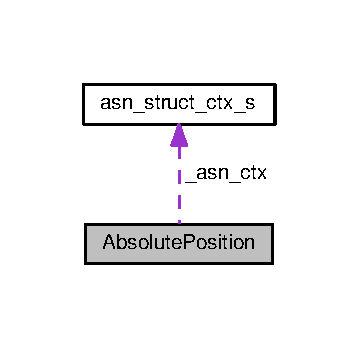
\includegraphics[width=172pt]{structAbsolutePosition__coll__graph}
\end{center}
\end{figure}
\subsection*{Public Attributes}
\begin{DoxyCompactItemize}
\item 
Latitude\+\_\+t {\bfseries latitude}\hypertarget{structAbsolutePosition_ae303886fea2dcb552c00198f70b8b36c}{}\label{structAbsolutePosition_ae303886fea2dcb552c00198f70b8b36c}

\item 
Longitude\+\_\+t {\bfseries longitude}\hypertarget{structAbsolutePosition_a9991c445539d9d4f49a20e70c2c64cef}{}\label{structAbsolutePosition_a9991c445539d9d4f49a20e70c2c64cef}

\item 
\hyperlink{structasn__struct__ctx__s}{asn\+\_\+struct\+\_\+ctx\+\_\+t} {\bfseries \+\_\+asn\+\_\+ctx}\hypertarget{structAbsolutePosition_a74f770a0614465f88f00a7764a858525}{}\label{structAbsolutePosition_a74f770a0614465f88f00a7764a858525}

\end{DoxyCompactItemize}


The documentation for this struct was generated from the following file\+:\begin{DoxyCompactItemize}
\item 
include/aimsun\+\_\+extensions/\+V2\+X\+Framework/\+I\+T\+S-\/spec/Absolute\+Position.\+h\end{DoxyCompactItemize}

\hypertarget{structAbsolutePositionWAltitude}{}\section{Absolute\+Position\+W\+Altitude Struct Reference}
\label{structAbsolutePositionWAltitude}\index{Absolute\+Position\+W\+Altitude@{Absolute\+Position\+W\+Altitude}}


Collaboration diagram for Absolute\+Position\+W\+Altitude\+:\nopagebreak
\begin{figure}[H]
\begin{center}
\leavevmode
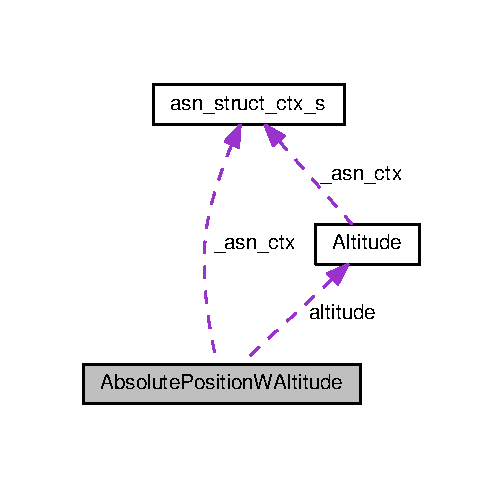
\includegraphics[width=242pt]{structAbsolutePositionWAltitude__coll__graph}
\end{center}
\end{figure}
\subsection*{Public Attributes}
\begin{DoxyCompactItemize}
\item 
Latitude\+\_\+t {\bfseries latitude}\hypertarget{structAbsolutePositionWAltitude_a76d49a7c3f65e73f667fa3f69351892b}{}\label{structAbsolutePositionWAltitude_a76d49a7c3f65e73f667fa3f69351892b}

\item 
Longitude\+\_\+t {\bfseries longitude}\hypertarget{structAbsolutePositionWAltitude_a81b17381c5f86c2163d1f1b26a345c59}{}\label{structAbsolutePositionWAltitude_a81b17381c5f86c2163d1f1b26a345c59}

\item 
\hyperlink{structAltitude}{Altitude\+\_\+t} {\bfseries altitude}\hypertarget{structAbsolutePositionWAltitude_a8a8a31cfa85a6644f8e87b9769c0ea61}{}\label{structAbsolutePositionWAltitude_a8a8a31cfa85a6644f8e87b9769c0ea61}

\item 
\hyperlink{structasn__struct__ctx__s}{asn\+\_\+struct\+\_\+ctx\+\_\+t} {\bfseries \+\_\+asn\+\_\+ctx}\hypertarget{structAbsolutePositionWAltitude_a6983ea6a5f4f8901a244f0c365f222a6}{}\label{structAbsolutePositionWAltitude_a6983ea6a5f4f8901a244f0c365f222a6}

\end{DoxyCompactItemize}


The documentation for this struct was generated from the following file\+:\begin{DoxyCompactItemize}
\item 
include/aimsun\+\_\+extensions/\+V2\+X\+Framework/\+I\+T\+S-\/spec/Absolute\+Position\+W\+Altitude.\+h\end{DoxyCompactItemize}

\hypertarget{structActionID}{}\section{Action\+ID Struct Reference}
\label{structActionID}\index{Action\+ID@{Action\+ID}}


Collaboration diagram for Action\+ID\+:\nopagebreak
\begin{figure}[H]
\begin{center}
\leavevmode
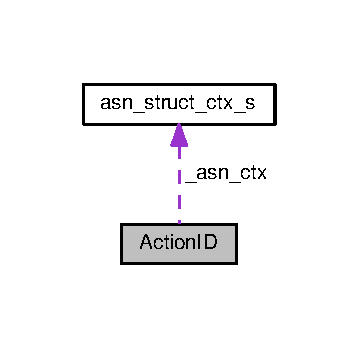
\includegraphics[width=172pt]{structActionID__coll__graph}
\end{center}
\end{figure}
\subsection*{Public Attributes}
\begin{DoxyCompactItemize}
\item 
Station\+I\+D\+\_\+t {\bfseries originating\+Station\+ID}\hypertarget{structActionID_a29ecab1361223b12ff09aaebdc54a42e}{}\label{structActionID_a29ecab1361223b12ff09aaebdc54a42e}

\item 
Sequence\+Number\+\_\+t {\bfseries sequence\+Number}\hypertarget{structActionID_a919dcd18229695bde2389d910c3d6aa3}{}\label{structActionID_a919dcd18229695bde2389d910c3d6aa3}

\item 
\hyperlink{structasn__struct__ctx__s}{asn\+\_\+struct\+\_\+ctx\+\_\+t} {\bfseries \+\_\+asn\+\_\+ctx}\hypertarget{structActionID_aae2526cb3cb1e7fa83c19e6d2a4ac321}{}\label{structActionID_aae2526cb3cb1e7fa83c19e6d2a4ac321}

\end{DoxyCompactItemize}


The documentation for this struct was generated from the following file\+:\begin{DoxyCompactItemize}
\item 
include/aimsun\+\_\+extensions/\+V2\+X\+Framework/\+I\+T\+S-\/spec/Action\+I\+D.\+h\end{DoxyCompactItemize}

\hypertarget{structAdvisorySpeed}{}\section{Advisory\+Speed Struct Reference}
\label{structAdvisorySpeed}\index{Advisory\+Speed@{Advisory\+Speed}}


Collaboration diagram for Advisory\+Speed\+:\nopagebreak
\begin{figure}[H]
\begin{center}
\leavevmode
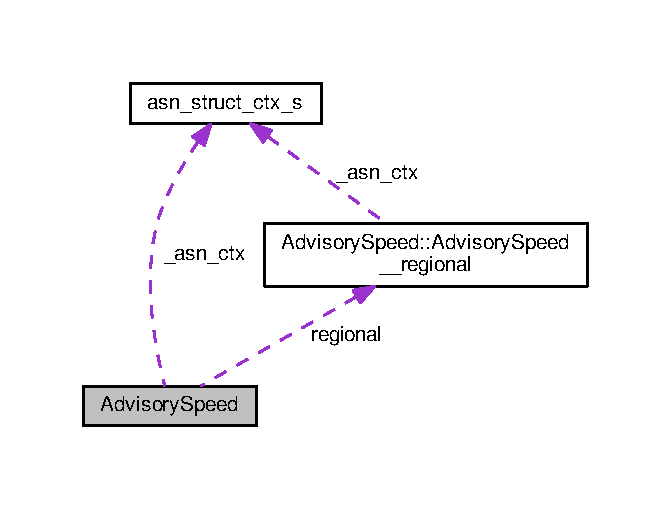
\includegraphics[width=322pt]{structAdvisorySpeed__coll__graph}
\end{center}
\end{figure}
\subsection*{Classes}
\begin{DoxyCompactItemize}
\item 
struct \hyperlink{structAdvisorySpeed_1_1AdvisorySpeed____regional}{Advisory\+Speed\+\_\+\+\_\+regional}
\end{DoxyCompactItemize}
\subsection*{Public Attributes}
\begin{DoxyCompactItemize}
\item 
Advisory\+Speed\+Type\+\_\+t {\bfseries type}\hypertarget{structAdvisorySpeed_a764accba96692fe68bc0a8d783a3d831}{}\label{structAdvisorySpeed_a764accba96692fe68bc0a8d783a3d831}

\item 
Speed\+Advice\+\_\+t $\ast$ {\bfseries speed}\hypertarget{structAdvisorySpeed_aaa81ebae74a2c0bff13f61f23c21f8a0}{}\label{structAdvisorySpeed_aaa81ebae74a2c0bff13f61f23c21f8a0}

\item 
Speed\+Confidence\+\_\+t $\ast$ {\bfseries confidence}\hypertarget{structAdvisorySpeed_aafa1266bb3ad181d7bf24ffea4a790a5}{}\label{structAdvisorySpeed_aafa1266bb3ad181d7bf24ffea4a790a5}

\item 
Zone\+Length\+\_\+t $\ast$ {\bfseries distance}\hypertarget{structAdvisorySpeed_a3bbbaecc721df88cc190b7c65da6496b}{}\label{structAdvisorySpeed_a3bbbaecc721df88cc190b7c65da6496b}

\item 
Restriction\+Class\+I\+D\+\_\+t $\ast$ {\bfseries Class}\hypertarget{structAdvisorySpeed_a151349f94c08d71e06fd76fd8db08ae3}{}\label{structAdvisorySpeed_a151349f94c08d71e06fd76fd8db08ae3}

\item 
struct \hyperlink{structAdvisorySpeed_1_1AdvisorySpeed____regional}{Advisory\+Speed\+::\+Advisory\+Speed\+\_\+\+\_\+regional} $\ast$ {\bfseries regional}\hypertarget{structAdvisorySpeed_a2f332ca0ed4422d9cab1dca89fc9a325}{}\label{structAdvisorySpeed_a2f332ca0ed4422d9cab1dca89fc9a325}

\item 
\hyperlink{structasn__struct__ctx__s}{asn\+\_\+struct\+\_\+ctx\+\_\+t} {\bfseries \+\_\+asn\+\_\+ctx}\hypertarget{structAdvisorySpeed_a47cc4c24645c8a03ed178f4d3e2e0970}{}\label{structAdvisorySpeed_a47cc4c24645c8a03ed178f4d3e2e0970}

\end{DoxyCompactItemize}


The documentation for this struct was generated from the following file\+:\begin{DoxyCompactItemize}
\item 
include/aimsun\+\_\+extensions/\+V2\+X\+Framework/\+I\+T\+S-\/spec/Advisory\+Speed.\+h\end{DoxyCompactItemize}

\hypertarget{structAdvisorySpeed_1_1AdvisorySpeed____regional}{}\section{Advisory\+Speed\+:\+:Advisory\+Speed\+\_\+\+\_\+regional Struct Reference}
\label{structAdvisorySpeed_1_1AdvisorySpeed____regional}\index{Advisory\+Speed\+::\+Advisory\+Speed\+\_\+\+\_\+regional@{Advisory\+Speed\+::\+Advisory\+Speed\+\_\+\+\_\+regional}}


Collaboration diagram for Advisory\+Speed\+:\+:Advisory\+Speed\+\_\+\+\_\+regional\+:\nopagebreak
\begin{figure}[H]
\begin{center}
\leavevmode
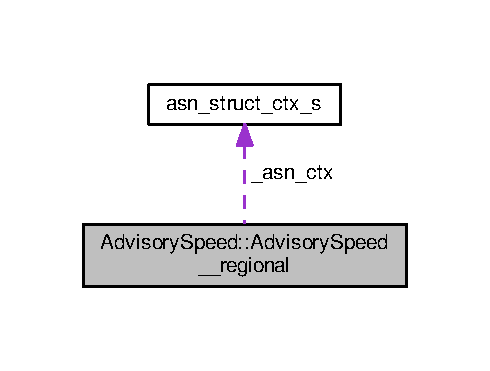
\includegraphics[width=235pt]{structAdvisorySpeed_1_1AdvisorySpeed____regional__coll__graph}
\end{center}
\end{figure}
\subsection*{Public Member Functions}
\begin{DoxyCompactItemize}
\item 
{\bfseries A\+\_\+\+S\+E\+Q\+U\+E\+N\+C\+E\+\_\+\+OF} (struct Regional\+Extension) list\hypertarget{structAdvisorySpeed_1_1AdvisorySpeed____regional_a65efef43fa873a07fb456e4ca2afb96c}{}\label{structAdvisorySpeed_1_1AdvisorySpeed____regional_a65efef43fa873a07fb456e4ca2afb96c}

\end{DoxyCompactItemize}
\subsection*{Public Attributes}
\begin{DoxyCompactItemize}
\item 
\hyperlink{structasn__struct__ctx__s}{asn\+\_\+struct\+\_\+ctx\+\_\+t} {\bfseries \+\_\+asn\+\_\+ctx}\hypertarget{structAdvisorySpeed_1_1AdvisorySpeed____regional_a63aed415ac6943050e04923709d349ee}{}\label{structAdvisorySpeed_1_1AdvisorySpeed____regional_a63aed415ac6943050e04923709d349ee}

\end{DoxyCompactItemize}


The documentation for this struct was generated from the following file\+:\begin{DoxyCompactItemize}
\item 
include/aimsun\+\_\+extensions/\+V2\+X\+Framework/\+I\+T\+S-\/spec/Advisory\+Speed.\+h\end{DoxyCompactItemize}

\hypertarget{structAdvisorySpeedList}{}\section{Advisory\+Speed\+List Struct Reference}
\label{structAdvisorySpeedList}\index{Advisory\+Speed\+List@{Advisory\+Speed\+List}}


Collaboration diagram for Advisory\+Speed\+List\+:\nopagebreak
\begin{figure}[H]
\begin{center}
\leavevmode
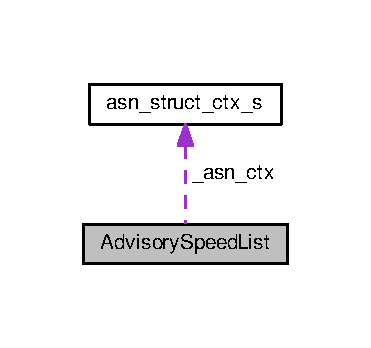
\includegraphics[width=178pt]{structAdvisorySpeedList__coll__graph}
\end{center}
\end{figure}
\subsection*{Public Member Functions}
\begin{DoxyCompactItemize}
\item 
{\bfseries A\+\_\+\+S\+E\+Q\+U\+E\+N\+C\+E\+\_\+\+OF} (struct \hyperlink{structAdvisorySpeed}{Advisory\+Speed}) list\hypertarget{structAdvisorySpeedList_ab8899d68bec7f62a6d62017a8e5d2cd3}{}\label{structAdvisorySpeedList_ab8899d68bec7f62a6d62017a8e5d2cd3}

\end{DoxyCompactItemize}
\subsection*{Public Attributes}
\begin{DoxyCompactItemize}
\item 
\hyperlink{structasn__struct__ctx__s}{asn\+\_\+struct\+\_\+ctx\+\_\+t} {\bfseries \+\_\+asn\+\_\+ctx}\hypertarget{structAdvisorySpeedList_af7e3a9c19d4a99f2ec2115fec19f10f7}{}\label{structAdvisorySpeedList_af7e3a9c19d4a99f2ec2115fec19f10f7}

\end{DoxyCompactItemize}


The documentation for this struct was generated from the following file\+:\begin{DoxyCompactItemize}
\item 
include/aimsun\+\_\+extensions/\+V2\+X\+Framework/\+I\+T\+S-\/spec/Advisory\+Speed\+List.\+h\end{DoxyCompactItemize}

\hypertarget{classADynamicAgent}{}\section{A\+Dynamic\+Agent Class Reference}
\label{classADynamicAgent}\index{A\+Dynamic\+Agent@{A\+Dynamic\+Agent}}


Get and set information from/to the Aimsun objects (including vehicles)  




{\ttfamily \#include $<$A\+Dynamic\+Agent.\+h$>$}



Inheritance diagram for A\+Dynamic\+Agent\+:\nopagebreak
\begin{figure}[H]
\begin{center}
\leavevmode
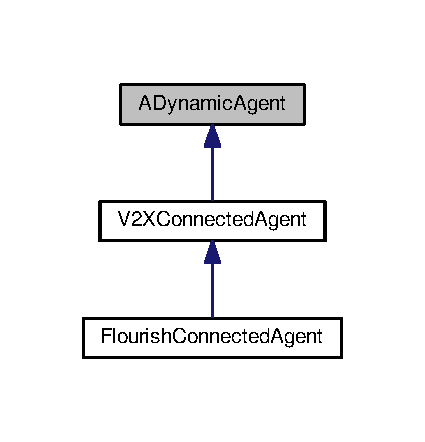
\includegraphics[width=204pt]{classADynamicAgent__inherit__graph}
\end{center}
\end{figure}
\subsection*{Public Member Functions}
\begin{DoxyCompactItemize}
\item 
\hyperlink{classADynamicAgent_a6535a8f571086793727c30b387c4883d}{A\+Dynamic\+Agent} (quint32 idhandler, D\+T\+A\+Veh $\ast$an\+Agent)
\begin{DoxyCompactList}\small\item\em Constructor. \end{DoxyCompactList}\item 
virtual \hyperlink{classADynamicAgent_ae1ba3cb111cb30562ad37df2aa0cda77}{$\sim$\+A\+Dynamic\+Agent} ()\hypertarget{classADynamicAgent_ae1ba3cb111cb30562ad37df2aa0cda77}{}\label{classADynamicAgent_ae1ba3cb111cb30562ad37df2aa0cda77}

\begin{DoxyCompactList}\small\item\em Deconstructor. \end{DoxyCompactList}\item 
virtual void \hyperlink{classADynamicAgent_a44aacef8be0302f2edc528a6b96168f7}{get\+State} (double time, double time\+Sta)=0
\begin{DoxyCompactList}\small\item\em Will be called by Aimsun simulator for every simulation step. \end{DoxyCompactList}\item 
virtual void \hyperlink{classADynamicAgent_ae52606684f790a26d46861ea21e932e7}{set\+State} (double time, double time\+Sta)=0
\begin{DoxyCompactList}\small\item\em Will be called by Aimsun simulator for every simulation step. \end{DoxyCompactList}\item 
int \hyperlink{classADynamicAgent_afaf6756338d00b2448776747ad00ea65}{get\+Id} () const 
\item 
int \hyperlink{classADynamicAgent_a9ca35fea075e20e491e493d9fd44df92}{get\+Veh\+Type} () const 
\item 
double \hyperlink{classADynamicAgent_acf478908f7f973585b5be726581421ac}{get\+Length} () const 
\item 
double \hyperlink{classADynamicAgent_a1193101357f3a12c4ba71965960c07ca}{get\+Width} () const 
\item 
double \hyperlink{classADynamicAgent_a59ef63d722e335a71a7b6a0df0d71ee4}{get\+Max\+Acceleration} () const 
\item 
double \hyperlink{classADynamicAgent_aace95766f8809611d1031b979fa8a337}{get\+Normal\+Deceleration} () const 
\item 
double \hyperlink{classADynamicAgent_a853f42ee7434c44c3c69c4151aeec7ff}{get\+Max\+Deceleration} () const 
\item 
double \hyperlink{classADynamicAgent_ab6af88406508481aee9ea2ed6acea157}{get\+Clearance} () const 
\item 
double \hyperlink{classADynamicAgent_a4d9313c66b0b8f000d294f7055211488}{get\+Sensitivity\+Factor} () const 
\item 
double \hyperlink{classADynamicAgent_adae57adcd692c56f1660dd95c2c827fa}{get\+Minimum\+Headway} () const 
\item 
bool \hyperlink{classADynamicAgent_af9a306fbf63c42dafdb3e5c9fc16cd40}{get\+Coordinates} (double $\ast$xfront, double $\ast$yfront, double $\ast$zfront, double $\ast$xback, double $\ast$yback, double $\ast$zback) const 
\item 
double \hyperlink{classADynamicAgent_ad6fc5e3ac38f74264be2203a00372f86}{get\+Free\+Flow\+Speed} () const 
\item 
double \hyperlink{classADynamicAgent_a9f6f908d8ea87021027677929d0e35ec}{get\+Speed} () const 
\item 
double \hyperlink{classADynamicAgent_a8896cb6d238d2babc6a0666aa57aca3f}{get\+Acceleration} () const 
\item 
double \hyperlink{classADynamicAgent_a0ad74bbe2e59ea63941b4dd34807b2aa}{get\+Heading} () const 
\item 
D\+T\+A\+Vehicle\+Type $\ast$ \hyperlink{classADynamicAgent_a40f4d4c543dd62607d349aa21d35de43}{get\+Vehicle\+Type} () const 
\end{DoxyCompactItemize}


\subsection{Detailed Description}
Get and set information from/to the Aimsun objects (including vehicles) 

The two methods, which are called in a middle of the simulation steps, are\+:


\begin{DoxyItemize}
\item The get\+State method, will be called by Aimsun simulator for every simulation step.
\item The set\+State method, will be called by Aimsun simulator for every simulation step.
\end{DoxyItemize}

Please remember that no order of call is guaranty between different updates. The other methods are getters for various vehicle properties, and they resolve to the internal agent in Aimsun. 

\subsection{Constructor \& Destructor Documentation}
\index{A\+Dynamic\+Agent@{A\+Dynamic\+Agent}!A\+Dynamic\+Agent@{A\+Dynamic\+Agent}}
\index{A\+Dynamic\+Agent@{A\+Dynamic\+Agent}!A\+Dynamic\+Agent@{A\+Dynamic\+Agent}}
\subsubsection[{\texorpdfstring{A\+Dynamic\+Agent(quint32 idhandler, D\+T\+A\+Veh $\ast$an\+Agent)}{ADynamicAgent(quint32 idhandler, DTAVeh *anAgent)}}]{\setlength{\rightskip}{0pt plus 5cm}A\+Dynamic\+Agent\+::\+A\+Dynamic\+Agent (
\begin{DoxyParamCaption}
\item[{quint32}]{idhandler, }
\item[{D\+T\+A\+Veh $\ast$}]{an\+Agent}
\end{DoxyParamCaption}
)}\hypertarget{classADynamicAgent_a6535a8f571086793727c30b387c4883d}{}\label{classADynamicAgent_a6535a8f571086793727c30b387c4883d}


Constructor. 


\begin{DoxyParams}{Parameters}
{\em idhandler} & Unique id of the agent (equivalent to call get\+Id) \\
\hline
{\em an\+Agent} & Opaque pointer for Aimsun agent \\
\hline
\end{DoxyParams}


\subsection{Member Function Documentation}
\index{A\+Dynamic\+Agent@{A\+Dynamic\+Agent}!get\+Acceleration@{get\+Acceleration}}
\index{get\+Acceleration@{get\+Acceleration}!A\+Dynamic\+Agent@{A\+Dynamic\+Agent}}
\subsubsection[{\texorpdfstring{get\+Acceleration() const }{getAcceleration() const }}]{\setlength{\rightskip}{0pt plus 5cm}double A\+Dynamic\+Agent\+::get\+Acceleration (
\begin{DoxyParamCaption}
{}
\end{DoxyParamCaption}
) const}\hypertarget{classADynamicAgent_a8896cb6d238d2babc6a0666aa57aca3f}{}\label{classADynamicAgent_a8896cb6d238d2babc6a0666aa57aca3f}
\begin{DoxyReturn}{Returns}
The current acceleration/deceleration of the vehicle (m/s2) 
\end{DoxyReturn}
\index{A\+Dynamic\+Agent@{A\+Dynamic\+Agent}!get\+Clearance@{get\+Clearance}}
\index{get\+Clearance@{get\+Clearance}!A\+Dynamic\+Agent@{A\+Dynamic\+Agent}}
\subsubsection[{\texorpdfstring{get\+Clearance() const }{getClearance() const }}]{\setlength{\rightskip}{0pt plus 5cm}double A\+Dynamic\+Agent\+::get\+Clearance (
\begin{DoxyParamCaption}
{}
\end{DoxyParamCaption}
) const}\hypertarget{classADynamicAgent_ab6af88406508481aee9ea2ed6acea157}{}\label{classADynamicAgent_ab6af88406508481aee9ea2ed6acea157}
\begin{DoxyReturn}{Returns}
The clearance space (Minimum gap) of the vehicle as defined in the vehicle type (m) 
\end{DoxyReturn}
\index{A\+Dynamic\+Agent@{A\+Dynamic\+Agent}!get\+Coordinates@{get\+Coordinates}}
\index{get\+Coordinates@{get\+Coordinates}!A\+Dynamic\+Agent@{A\+Dynamic\+Agent}}
\subsubsection[{\texorpdfstring{get\+Coordinates(double $\ast$xfront, double $\ast$yfront, double $\ast$zfront, double $\ast$xback, double $\ast$yback, double $\ast$zback) const }{getCoordinates(double *xfront, double *yfront, double *zfront, double *xback, double *yback, double *zback) const }}]{\setlength{\rightskip}{0pt plus 5cm}bool A\+Dynamic\+Agent\+::get\+Coordinates (
\begin{DoxyParamCaption}
\item[{double $\ast$}]{xfront, }
\item[{double $\ast$}]{yfront, }
\item[{double $\ast$}]{zfront, }
\item[{double $\ast$}]{xback, }
\item[{double $\ast$}]{yback, }
\item[{double $\ast$}]{zback}
\end{DoxyParamCaption}
) const}\hypertarget{classADynamicAgent_af9a306fbf63c42dafdb3e5c9fc16cd40}{}\label{classADynamicAgent_af9a306fbf63c42dafdb3e5c9fc16cd40}

\begin{DoxyParams}{Parameters}
{\em xfront} & T\+O\+DO \\
\hline
{\em yfront} & T\+O\+DO \\
\hline
{\em zfront} & T\+O\+DO \\
\hline
{\em xback} & T\+O\+DO \\
\hline
{\em yback} & T\+O\+DO \\
\hline
{\em zback} & T\+O\+DO \\
\hline
\end{DoxyParams}
\begin{DoxyReturn}{Returns}
The coordinates of the middle front point and middle back point 
\end{DoxyReturn}
\index{A\+Dynamic\+Agent@{A\+Dynamic\+Agent}!get\+Free\+Flow\+Speed@{get\+Free\+Flow\+Speed}}
\index{get\+Free\+Flow\+Speed@{get\+Free\+Flow\+Speed}!A\+Dynamic\+Agent@{A\+Dynamic\+Agent}}
\subsubsection[{\texorpdfstring{get\+Free\+Flow\+Speed() const }{getFreeFlowSpeed() const }}]{\setlength{\rightskip}{0pt plus 5cm}double A\+Dynamic\+Agent\+::get\+Free\+Flow\+Speed (
\begin{DoxyParamCaption}
{}
\end{DoxyParamCaption}
) const}\hypertarget{classADynamicAgent_ad6fc5e3ac38f74264be2203a00372f86}{}\label{classADynamicAgent_ad6fc5e3ac38f74264be2203a00372f86}
\begin{DoxyReturn}{Returns}
The maximum Desired \hyperlink{structSpeed}{Speed} of the vehicle for the current lane (m/s) 
\end{DoxyReturn}
\index{A\+Dynamic\+Agent@{A\+Dynamic\+Agent}!get\+Heading@{get\+Heading}}
\index{get\+Heading@{get\+Heading}!A\+Dynamic\+Agent@{A\+Dynamic\+Agent}}
\subsubsection[{\texorpdfstring{get\+Heading() const }{getHeading() const }}]{\setlength{\rightskip}{0pt plus 5cm}double A\+Dynamic\+Agent\+::get\+Heading (
\begin{DoxyParamCaption}
{}
\end{DoxyParamCaption}
) const}\hypertarget{classADynamicAgent_a0ad74bbe2e59ea63941b4dd34807b2aa}{}\label{classADynamicAgent_a0ad74bbe2e59ea63941b4dd34807b2aa}
\begin{DoxyReturn}{Returns}
The heading express in angle \+: 0 North, 90 East, 180 South 270 West 
\end{DoxyReturn}
\index{A\+Dynamic\+Agent@{A\+Dynamic\+Agent}!get\+Id@{get\+Id}}
\index{get\+Id@{get\+Id}!A\+Dynamic\+Agent@{A\+Dynamic\+Agent}}
\subsubsection[{\texorpdfstring{get\+Id() const }{getId() const }}]{\setlength{\rightskip}{0pt plus 5cm}int A\+Dynamic\+Agent\+::get\+Id (
\begin{DoxyParamCaption}
{}
\end{DoxyParamCaption}
) const}\hypertarget{classADynamicAgent_afaf6756338d00b2448776747ad00ea65}{}\label{classADynamicAgent_afaf6756338d00b2448776747ad00ea65}
\begin{DoxyReturn}{Returns}
The Aimsun id vehicle assigned during the simulation 
\end{DoxyReturn}
\index{A\+Dynamic\+Agent@{A\+Dynamic\+Agent}!get\+Length@{get\+Length}}
\index{get\+Length@{get\+Length}!A\+Dynamic\+Agent@{A\+Dynamic\+Agent}}
\subsubsection[{\texorpdfstring{get\+Length() const }{getLength() const }}]{\setlength{\rightskip}{0pt plus 5cm}double A\+Dynamic\+Agent\+::get\+Length (
\begin{DoxyParamCaption}
{}
\end{DoxyParamCaption}
) const}\hypertarget{classADynamicAgent_acf478908f7f973585b5be726581421ac}{}\label{classADynamicAgent_acf478908f7f973585b5be726581421ac}
\begin{DoxyReturn}{Returns}
The length of the vehicle (meters) 
\end{DoxyReturn}
\index{A\+Dynamic\+Agent@{A\+Dynamic\+Agent}!get\+Max\+Acceleration@{get\+Max\+Acceleration}}
\index{get\+Max\+Acceleration@{get\+Max\+Acceleration}!A\+Dynamic\+Agent@{A\+Dynamic\+Agent}}
\subsubsection[{\texorpdfstring{get\+Max\+Acceleration() const }{getMaxAcceleration() const }}]{\setlength{\rightskip}{0pt plus 5cm}double A\+Dynamic\+Agent\+::get\+Max\+Acceleration (
\begin{DoxyParamCaption}
{}
\end{DoxyParamCaption}
) const}\hypertarget{classADynamicAgent_a59ef63d722e335a71a7b6a0df0d71ee4}{}\label{classADynamicAgent_a59ef63d722e335a71a7b6a0df0d71ee4}
\begin{DoxyReturn}{Returns}
The Maximum acceleration of the vehicle as specified in the vehicle type considering local variations (m/s2) 
\end{DoxyReturn}
\index{A\+Dynamic\+Agent@{A\+Dynamic\+Agent}!get\+Max\+Deceleration@{get\+Max\+Deceleration}}
\index{get\+Max\+Deceleration@{get\+Max\+Deceleration}!A\+Dynamic\+Agent@{A\+Dynamic\+Agent}}
\subsubsection[{\texorpdfstring{get\+Max\+Deceleration() const }{getMaxDeceleration() const }}]{\setlength{\rightskip}{0pt plus 5cm}double A\+Dynamic\+Agent\+::get\+Max\+Deceleration (
\begin{DoxyParamCaption}
{}
\end{DoxyParamCaption}
) const}\hypertarget{classADynamicAgent_a853f42ee7434c44c3c69c4151aeec7ff}{}\label{classADynamicAgent_a853f42ee7434c44c3c69c4151aeec7ff}
\begin{DoxyReturn}{Returns}
The Maximum (emergency) deceleration of the vehicle as specified in the vehicle type considering local variations (m/s2) 
\end{DoxyReturn}
\index{A\+Dynamic\+Agent@{A\+Dynamic\+Agent}!get\+Minimum\+Headway@{get\+Minimum\+Headway}}
\index{get\+Minimum\+Headway@{get\+Minimum\+Headway}!A\+Dynamic\+Agent@{A\+Dynamic\+Agent}}
\subsubsection[{\texorpdfstring{get\+Minimum\+Headway() const }{getMinimumHeadway() const }}]{\setlength{\rightskip}{0pt plus 5cm}double A\+Dynamic\+Agent\+::get\+Minimum\+Headway (
\begin{DoxyParamCaption}
{}
\end{DoxyParamCaption}
) const}\hypertarget{classADynamicAgent_adae57adcd692c56f1660dd95c2c827fa}{}\label{classADynamicAgent_adae57adcd692c56f1660dd95c2c827fa}
\begin{DoxyReturn}{Returns}
The Minimum Headway (also know as Gap) in font of the vehicle as defined in the vehicle type (s) 
\end{DoxyReturn}
\index{A\+Dynamic\+Agent@{A\+Dynamic\+Agent}!get\+Normal\+Deceleration@{get\+Normal\+Deceleration}}
\index{get\+Normal\+Deceleration@{get\+Normal\+Deceleration}!A\+Dynamic\+Agent@{A\+Dynamic\+Agent}}
\subsubsection[{\texorpdfstring{get\+Normal\+Deceleration() const }{getNormalDeceleration() const }}]{\setlength{\rightskip}{0pt plus 5cm}double A\+Dynamic\+Agent\+::get\+Normal\+Deceleration (
\begin{DoxyParamCaption}
{}
\end{DoxyParamCaption}
) const}\hypertarget{classADynamicAgent_aace95766f8809611d1031b979fa8a337}{}\label{classADynamicAgent_aace95766f8809611d1031b979fa8a337}
\begin{DoxyReturn}{Returns}
The Nomal deceleration of the vehicle as specified in the vehicle type considering local variations (m/s2) 
\end{DoxyReturn}
\index{A\+Dynamic\+Agent@{A\+Dynamic\+Agent}!get\+Sensitivity\+Factor@{get\+Sensitivity\+Factor}}
\index{get\+Sensitivity\+Factor@{get\+Sensitivity\+Factor}!A\+Dynamic\+Agent@{A\+Dynamic\+Agent}}
\subsubsection[{\texorpdfstring{get\+Sensitivity\+Factor() const }{getSensitivityFactor() const }}]{\setlength{\rightskip}{0pt plus 5cm}double A\+Dynamic\+Agent\+::get\+Sensitivity\+Factor (
\begin{DoxyParamCaption}
{}
\end{DoxyParamCaption}
) const}\hypertarget{classADynamicAgent_a4d9313c66b0b8f000d294f7055211488}{}\label{classADynamicAgent_a4d9313c66b0b8f000d294f7055211488}
\begin{DoxyReturn}{Returns}
The sensitivity Factor to Leader´s deceleration as defined in the vehicle type 
\end{DoxyReturn}
\index{A\+Dynamic\+Agent@{A\+Dynamic\+Agent}!get\+Speed@{get\+Speed}}
\index{get\+Speed@{get\+Speed}!A\+Dynamic\+Agent@{A\+Dynamic\+Agent}}
\subsubsection[{\texorpdfstring{get\+Speed() const }{getSpeed() const }}]{\setlength{\rightskip}{0pt plus 5cm}double A\+Dynamic\+Agent\+::get\+Speed (
\begin{DoxyParamCaption}
{}
\end{DoxyParamCaption}
) const}\hypertarget{classADynamicAgent_a9f6f908d8ea87021027677929d0e35ec}{}\label{classADynamicAgent_a9f6f908d8ea87021027677929d0e35ec}
\begin{DoxyReturn}{Returns}
The current speed of the vehicle (m/s) 
\end{DoxyReturn}
\index{A\+Dynamic\+Agent@{A\+Dynamic\+Agent}!get\+State@{get\+State}}
\index{get\+State@{get\+State}!A\+Dynamic\+Agent@{A\+Dynamic\+Agent}}
\subsubsection[{\texorpdfstring{get\+State(double time, double time\+Sta)=0}{getState(double time, double timeSta)=0}}]{\setlength{\rightskip}{0pt plus 5cm}virtual void A\+Dynamic\+Agent\+::get\+State (
\begin{DoxyParamCaption}
\item[{double}]{time, }
\item[{double}]{time\+Sta}
\end{DoxyParamCaption}
)\hspace{0.3cm}{\ttfamily [pure virtual]}}\hypertarget{classADynamicAgent_a44aacef8be0302f2edc528a6b96168f7}{}\label{classADynamicAgent_a44aacef8be0302f2edc528a6b96168f7}


Will be called by Aimsun simulator for every simulation step. 


\begin{DoxyParams}{Parameters}
{\em time} & Simulation time \\
\hline
{\em time\+Sta} & Time from 00\+:00.\+00 (midnight) of the current day \\
\hline
\end{DoxyParams}


Implemented in \hyperlink{classV2XConnectedAgent_a3c7e42f33c9cb3c25cd2374063f151da}{V2\+X\+Connected\+Agent}.

\index{A\+Dynamic\+Agent@{A\+Dynamic\+Agent}!get\+Vehicle\+Type@{get\+Vehicle\+Type}}
\index{get\+Vehicle\+Type@{get\+Vehicle\+Type}!A\+Dynamic\+Agent@{A\+Dynamic\+Agent}}
\subsubsection[{\texorpdfstring{get\+Vehicle\+Type() const }{getVehicleType() const }}]{\setlength{\rightskip}{0pt plus 5cm}D\+T\+A\+Vehicle\+Type$\ast$ A\+Dynamic\+Agent\+::get\+Vehicle\+Type (
\begin{DoxyParamCaption}
{}
\end{DoxyParamCaption}
) const}\hypertarget{classADynamicAgent_a40f4d4c543dd62607d349aa21d35de43}{}\label{classADynamicAgent_a40f4d4c543dd62607d349aa21d35de43}
\begin{DoxyReturn}{Returns}
The vehicle type 
\end{DoxyReturn}
\index{A\+Dynamic\+Agent@{A\+Dynamic\+Agent}!get\+Veh\+Type@{get\+Veh\+Type}}
\index{get\+Veh\+Type@{get\+Veh\+Type}!A\+Dynamic\+Agent@{A\+Dynamic\+Agent}}
\subsubsection[{\texorpdfstring{get\+Veh\+Type() const }{getVehType() const }}]{\setlength{\rightskip}{0pt plus 5cm}int A\+Dynamic\+Agent\+::get\+Veh\+Type (
\begin{DoxyParamCaption}
{}
\end{DoxyParamCaption}
) const}\hypertarget{classADynamicAgent_a9ca35fea075e20e491e493d9fd44df92}{}\label{classADynamicAgent_a9ca35fea075e20e491e493d9fd44df92}
\begin{DoxyReturn}{Returns}
the Aimsun Vehicle Type of the vehicle 
\end{DoxyReturn}
\index{A\+Dynamic\+Agent@{A\+Dynamic\+Agent}!get\+Width@{get\+Width}}
\index{get\+Width@{get\+Width}!A\+Dynamic\+Agent@{A\+Dynamic\+Agent}}
\subsubsection[{\texorpdfstring{get\+Width() const }{getWidth() const }}]{\setlength{\rightskip}{0pt plus 5cm}double A\+Dynamic\+Agent\+::get\+Width (
\begin{DoxyParamCaption}
{}
\end{DoxyParamCaption}
) const}\hypertarget{classADynamicAgent_a1193101357f3a12c4ba71965960c07ca}{}\label{classADynamicAgent_a1193101357f3a12c4ba71965960c07ca}
\begin{DoxyReturn}{Returns}
The width of the vehicle (meters) 
\end{DoxyReturn}
\index{A\+Dynamic\+Agent@{A\+Dynamic\+Agent}!set\+State@{set\+State}}
\index{set\+State@{set\+State}!A\+Dynamic\+Agent@{A\+Dynamic\+Agent}}
\subsubsection[{\texorpdfstring{set\+State(double time, double time\+Sta)=0}{setState(double time, double timeSta)=0}}]{\setlength{\rightskip}{0pt plus 5cm}virtual void A\+Dynamic\+Agent\+::set\+State (
\begin{DoxyParamCaption}
\item[{double}]{time, }
\item[{double}]{time\+Sta}
\end{DoxyParamCaption}
)\hspace{0.3cm}{\ttfamily [pure virtual]}}\hypertarget{classADynamicAgent_ae52606684f790a26d46861ea21e932e7}{}\label{classADynamicAgent_ae52606684f790a26d46861ea21e932e7}


Will be called by Aimsun simulator for every simulation step. 


\begin{DoxyParams}{Parameters}
{\em time} & Simulation time \\
\hline
{\em time\+Sta} & Time from 00\+:00.\+00 (midnight) of the current day \\
\hline
\end{DoxyParams}


Implemented in \hyperlink{classV2XConnectedAgent_a771b23c38e5ac18d0219d4d8fefccb5a}{V2\+X\+Connected\+Agent}.



The documentation for this class was generated from the following file\+:\begin{DoxyCompactItemize}
\item 
include/core/\+A\+N\+G\+\_\+\+D\+T\+A/\+A\+Dynamic\+A\+P\+I/A\+Dynamic\+Agent.\+h\end{DoxyCompactItemize}

\hypertarget{classADynamicAPI}{}\section{A\+Dynamic\+A\+PI Class Reference}
\label{classADynamicAPI}\index{A\+Dynamic\+A\+PI@{A\+Dynamic\+A\+PI}}


A communication framework between Aimsun and an external plugin.  




{\ttfamily \#include $<$A\+Dynamic\+A\+P\+I.\+h$>$}



Inheritance diagram for A\+Dynamic\+A\+PI\+:\nopagebreak
\begin{figure}[H]
\begin{center}
\leavevmode
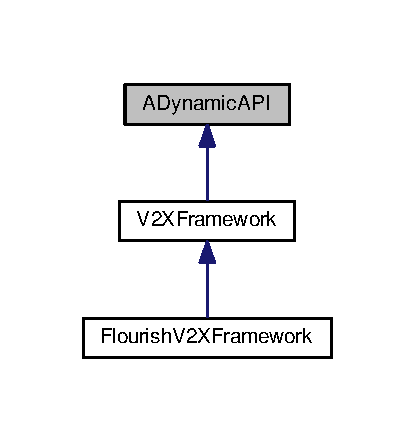
\includegraphics[width=199pt]{classADynamicAPI__inherit__graph}
\end{center}
\end{figure}
\subsection*{Public Member Functions}
\begin{DoxyCompactItemize}
\item 
\hyperlink{classADynamicAPI_a0791cdc47d83c1c2cb8fcca9318ea1b4}{A\+Dynamic\+A\+PI} (\hyperlink{classADynamicAPISetup}{A\+Dynamic\+A\+P\+I\+Setup} \&setup)
\begin{DoxyCompactList}\small\item\em \hyperlink{classADynamicAPI}{A\+Dynamic\+A\+PI} Constructor. \end{DoxyCompactList}\item 
virtual \hyperlink{classADynamicAPI_a4f3e3112b0e1d679865e20c69597c2ba}{$\sim$\+A\+Dynamic\+A\+PI} ()\hypertarget{classADynamicAPI_a4f3e3112b0e1d679865e20c69597c2ba}{}\label{classADynamicAPI_a4f3e3112b0e1d679865e20c69597c2ba}

\begin{DoxyCompactList}\small\item\em Deconstructor. \end{DoxyCompactList}\item 
virtual \hyperlink{classADynamicAgent}{A\+Dynamic\+Agent} $\ast$ \hyperlink{classADynamicAPI_a9515f56fba44ad8f5aeaeca1b5091b14}{arrival\+New\+Vehicle} (quint32 id\+Handler, D\+T\+A\+Veh $\ast$agent)=0
\begin{DoxyCompactList}\small\item\em A vehicle enters the system. \end{DoxyCompactList}\item 
virtual void \hyperlink{classADynamicAPI_a6f4148dd485116a83caba071ea6a688f}{removed\+Vehicle} (quint32 id\+Handler, \hyperlink{classADynamicAgent}{A\+Dynamic\+Agent} $\ast$agent)=0
\begin{DoxyCompactList}\small\item\em A vehicle leaves the system. \end{DoxyCompactList}\item 
virtual void \hyperlink{classADynamicAPI_ab00f0ff26b69cae13d72d2d84cc8174b}{pre\+Update} (double time, double time\+Sta, double sim\+Step)=0
\begin{DoxyCompactList}\small\item\em Called before every simulation step (or simulation event) \end{DoxyCompactList}\item 
virtual void \hyperlink{classADynamicAPI_ab70821f058585820cfbc9287946642da}{post\+Update} (double time, double time\+Sta, double sim\+Step)=0
\begin{DoxyCompactList}\small\item\em Called after every simulation step (or simulation event) \end{DoxyCompactList}\end{DoxyCompactItemize}


\subsection{Detailed Description}
A communication framework between Aimsun and an external plugin. 

The objective of this class is to manage the communication between Aimsun simulator and this framework.

The user must rewrite its four virtual methods, which acts as a callbacks (the simulator will call these methods, and will use its return value).

For a detailed description, please look at the documentation of each method.

\begin{DoxySeeAlso}{See also}
\hyperlink{classADynamicAPI_a9515f56fba44ad8f5aeaeca1b5091b14}{arrival\+New\+Vehicle} 

\hyperlink{classADynamicAPI_a6f4148dd485116a83caba071ea6a688f}{removed\+Vehicle} 

\hyperlink{classADynamicAPI_ab00f0ff26b69cae13d72d2d84cc8174b}{pre\+Update} 

\hyperlink{classADynamicAPI_ab70821f058585820cfbc9287946642da}{post\+Update} 
\end{DoxySeeAlso}


\subsection{Constructor \& Destructor Documentation}
\index{A\+Dynamic\+A\+PI@{A\+Dynamic\+A\+PI}!A\+Dynamic\+A\+PI@{A\+Dynamic\+A\+PI}}
\index{A\+Dynamic\+A\+PI@{A\+Dynamic\+A\+PI}!A\+Dynamic\+A\+PI@{A\+Dynamic\+A\+PI}}
\subsubsection[{\texorpdfstring{A\+Dynamic\+A\+P\+I(\+A\+Dynamic\+A\+P\+I\+Setup \&setup)}{ADynamicAPI(ADynamicAPISetup &setup)}}]{\setlength{\rightskip}{0pt plus 5cm}A\+Dynamic\+A\+P\+I\+::\+A\+Dynamic\+A\+PI (
\begin{DoxyParamCaption}
\item[{{\bf A\+Dynamic\+A\+P\+I\+Setup} \&}]{setup}
\end{DoxyParamCaption}
)\hspace{0.3cm}{\ttfamily [inline]}}\hypertarget{classADynamicAPI_a0791cdc47d83c1c2cb8fcca9318ea1b4}{}\label{classADynamicAPI_a0791cdc47d83c1c2cb8fcca9318ea1b4}


\hyperlink{classADynamicAPI}{A\+Dynamic\+A\+PI} Constructor. 

The \hyperlink{classADynamicAPISetup}{A\+Dynamic\+A\+P\+I\+Setup} will always be valid (a copy can be made)


\begin{DoxyParams}{Parameters}
{\em setup} & The A\+PI setup interface \\
\hline
\end{DoxyParams}


\subsection{Member Function Documentation}
\index{A\+Dynamic\+A\+PI@{A\+Dynamic\+A\+PI}!arrival\+New\+Vehicle@{arrival\+New\+Vehicle}}
\index{arrival\+New\+Vehicle@{arrival\+New\+Vehicle}!A\+Dynamic\+A\+PI@{A\+Dynamic\+A\+PI}}
\subsubsection[{\texorpdfstring{arrival\+New\+Vehicle(quint32 id\+Handler, D\+T\+A\+Veh $\ast$agent)=0}{arrivalNewVehicle(quint32 idHandler, DTAVeh *agent)=0}}]{\setlength{\rightskip}{0pt plus 5cm}virtual {\bf A\+Dynamic\+Agent}$\ast$ A\+Dynamic\+A\+P\+I\+::arrival\+New\+Vehicle (
\begin{DoxyParamCaption}
\item[{quint32}]{id\+Handler, }
\item[{D\+T\+A\+Veh $\ast$}]{agent}
\end{DoxyParamCaption}
)\hspace{0.3cm}{\ttfamily [pure virtual]}}\hypertarget{classADynamicAPI_a9515f56fba44ad8f5aeaeca1b5091b14}{}\label{classADynamicAPI_a9515f56fba44ad8f5aeaeca1b5091b14}


A vehicle enters the system. 

It is called whenever a vehicle enters inside the system and should create a new vehicle. 
\begin{DoxyParams}{Parameters}
{\em id\+Handler} & Unique ID of the agent (it is equivalent to \hyperlink{classADynamicAgent_afaf6756338d00b2448776747ad00ea65}{A\+Dynamic\+Agent\+::get\+Id}) \\
\hline
{\em agent} & An opaque pointer representing the vehicle.\\
\hline
\end{DoxyParams}
\begin{DoxyReturn}{Returns}
A pointer to an \hyperlink{classADynamicAgent}{A\+Dynamic\+Agent} to be used by the simulator
\end{DoxyReturn}
An user outside Aimsun should never use this pointer directly. 

Implemented in \hyperlink{classFlourishV2XFramework_a47368514f7814d3d6db4cf8aaf049d3b}{Flourish\+V2\+X\+Framework}.

\index{A\+Dynamic\+A\+PI@{A\+Dynamic\+A\+PI}!post\+Update@{post\+Update}}
\index{post\+Update@{post\+Update}!A\+Dynamic\+A\+PI@{A\+Dynamic\+A\+PI}}
\subsubsection[{\texorpdfstring{post\+Update(double time, double time\+Sta, double sim\+Step)=0}{postUpdate(double time, double timeSta, double simStep)=0}}]{\setlength{\rightskip}{0pt plus 5cm}virtual void A\+Dynamic\+A\+P\+I\+::post\+Update (
\begin{DoxyParamCaption}
\item[{double}]{time, }
\item[{double}]{time\+Sta, }
\item[{double}]{sim\+Step}
\end{DoxyParamCaption}
)\hspace{0.3cm}{\ttfamily [pure virtual]}}\hypertarget{classADynamicAPI_ab70821f058585820cfbc9287946642da}{}\label{classADynamicAPI_ab70821f058585820cfbc9287946642da}


Called after every simulation step (or simulation event) 


\begin{DoxyParams}{Parameters}
{\em time} & Simulation time \\
\hline
{\em time\+Sta} & Time from 00\+:00.\+00 (midnight) of the current day \\
\hline
{\em sim\+Step} & Simulation step \\
\hline
\end{DoxyParams}


Implemented in \hyperlink{classFlourishV2XFramework_aa1417bf763cc7b9278df12dfda185010}{Flourish\+V2\+X\+Framework}.

\index{A\+Dynamic\+A\+PI@{A\+Dynamic\+A\+PI}!pre\+Update@{pre\+Update}}
\index{pre\+Update@{pre\+Update}!A\+Dynamic\+A\+PI@{A\+Dynamic\+A\+PI}}
\subsubsection[{\texorpdfstring{pre\+Update(double time, double time\+Sta, double sim\+Step)=0}{preUpdate(double time, double timeSta, double simStep)=0}}]{\setlength{\rightskip}{0pt plus 5cm}virtual void A\+Dynamic\+A\+P\+I\+::pre\+Update (
\begin{DoxyParamCaption}
\item[{double}]{time, }
\item[{double}]{time\+Sta, }
\item[{double}]{sim\+Step}
\end{DoxyParamCaption}
)\hspace{0.3cm}{\ttfamily [pure virtual]}}\hypertarget{classADynamicAPI_ab00f0ff26b69cae13d72d2d84cc8174b}{}\label{classADynamicAPI_ab00f0ff26b69cae13d72d2d84cc8174b}


Called before every simulation step (or simulation event) 


\begin{DoxyParams}{Parameters}
{\em time} & Simulation time \\
\hline
{\em time\+Sta} & Time from 00\+:00.\+00 (midnight) of the current day \\
\hline
{\em sim\+Step} & Simulation step \\
\hline
\end{DoxyParams}


Implemented in \hyperlink{classFlourishV2XFramework_a7dc6777db5dc693c67733e50af76c855}{Flourish\+V2\+X\+Framework}.

\index{A\+Dynamic\+A\+PI@{A\+Dynamic\+A\+PI}!removed\+Vehicle@{removed\+Vehicle}}
\index{removed\+Vehicle@{removed\+Vehicle}!A\+Dynamic\+A\+PI@{A\+Dynamic\+A\+PI}}
\subsubsection[{\texorpdfstring{removed\+Vehicle(quint32 id\+Handler, A\+Dynamic\+Agent $\ast$agent)=0}{removedVehicle(quint32 idHandler, ADynamicAgent *agent)=0}}]{\setlength{\rightskip}{0pt plus 5cm}virtual void A\+Dynamic\+A\+P\+I\+::removed\+Vehicle (
\begin{DoxyParamCaption}
\item[{quint32}]{id\+Handler, }
\item[{{\bf A\+Dynamic\+Agent} $\ast$}]{agent}
\end{DoxyParamCaption}
)\hspace{0.3cm}{\ttfamily [pure virtual]}}\hypertarget{classADynamicAPI_a6f4148dd485116a83caba071ea6a688f}{}\label{classADynamicAPI_a6f4148dd485116a83caba071ea6a688f}


A vehicle leaves the system. 

It is called when a vehicle leaves the system; the memory pointed by agent can be safely freed.


\begin{DoxyParams}{Parameters}
{\em id\+Handler} & Unique ID of the agent \\
\hline
{\em agent} & The agent pointer \\
\hline
\end{DoxyParams}


Implemented in \hyperlink{classFlourishV2XFramework_a60ff1aaea1448c9a05892597898c48a6}{Flourish\+V2\+X\+Framework}.



The documentation for this class was generated from the following file\+:\begin{DoxyCompactItemize}
\item 
include/core/\+A\+N\+G\+\_\+\+D\+T\+A/\+A\+Dynamic\+A\+P\+I/A\+Dynamic\+A\+P\+I.\+h\end{DoxyCompactItemize}

\hypertarget{classADynamicAPISetup}{}\section{A\+Dynamic\+A\+P\+I\+Setup Class Reference}
\label{classADynamicAPISetup}\index{A\+Dynamic\+A\+P\+I\+Setup@{A\+Dynamic\+A\+P\+I\+Setup}}


The interface between the internals of Aimsun with the outside.  




{\ttfamily \#include $<$A\+Dynamic\+A\+P\+I\+Setup.\+h$>$}

\subsection*{Classes}
\begin{DoxyCompactItemize}
\item 
struct \hyperlink{structADynamicAPISetup_1_1UserPreference}{User\+Preference}
\begin{DoxyCompactList}\small\item\em Define a preference for the attributes. \end{DoxyCompactList}\end{DoxyCompactItemize}
\subsection*{Public Types}
\begin{DoxyCompactItemize}
\item 
enum \hyperlink{classADynamicAPISetup_a0ffce2ed1acaeaf1f058fab833e375c3}{Type} \{ \\*
{\bfseries Invalid}, 
{\bfseries Map}, 
{\bfseries List}, 
{\bfseries String}, 
\\*
{\bfseries String\+List}, 
{\bfseries Font}, 
{\bfseries Pixmap}, 
{\bfseries Brush}, 
\\*
{\bfseries Rect}, 
{\bfseries Size}, 
{\bfseries Color}, 
{\bfseries Palette}, 
\\*
{\bfseries Color\+Group}, 
{\bfseries Icon\+Set}, 
{\bfseries Point}, 
{\bfseries Image}, 
\\*
{\bfseries Int}, 
{\bfseries U\+Int}, 
{\bfseries Bool}, 
{\bfseries Double}, 
\\*
{\bfseries C\+String}, 
{\bfseries Point\+Array}, 
{\bfseries Region}, 
{\bfseries Bitmap}, 
\\*
{\bfseries Cursor}, 
{\bfseries Size\+Policy}, 
{\bfseries Date}, 
{\bfseries Time}, 
\\*
{\bfseries Date\+Time}, 
{\bfseries Byte\+Array}, 
{\bfseries \+\_\+\+G\+K\+Object}, 
{\bfseries \+\_\+\+G\+K\+Segmented\+Attribute\+\_\+\+Obsolete}, 
\\*
{\bfseries \+\_\+\+G\+K\+Time\+Serie}, 
{\bfseries \+\_\+\+G\+K\+Enum}, 
{\bfseries \+\_\+\+G\+K\+Time\+Duration}, 
{\bfseries \+\_\+\+G\+K\+Object\+List}, 
\\*
{\bfseries \+\_\+\+G\+K\+Column}, 
{\bfseries \+\_\+\+G\+K\+Type}, 
{\bfseries \+\_\+\+G\+K\+Content}, 
{\bfseries File}, 
\\*
{\bfseries Void}, 
{\bfseries \+\_\+\+G\+K\+Normal\+Distribution\+Parameters}
 \}\hypertarget{classADynamicAPISetup_a0ffce2ed1acaeaf1f058fab833e375c3}{}\label{classADynamicAPISetup_a0ffce2ed1acaeaf1f058fab833e375c3}
\begin{DoxyCompactList}\small\item\em Available attribute types (copy pasted from G\+K\+Column) \end{DoxyCompactList}
\end{DoxyCompactItemize}
\subsection*{Public Member Functions}
\begin{DoxyCompactItemize}
\item 
\hyperlink{classADynamicAPISetup_a58135747ce3f1e21d9f1e385e9f6a662}{A\+Dynamic\+A\+P\+I\+Setup} (G\+K\+Model $\ast$handler\+Mod, G\+K\+Experiment $\ast$handler\+Exp)
\begin{DoxyCompactList}\small\item\em \hyperlink{classADynamicAPISetup}{A\+Dynamic\+A\+P\+I\+Setup} default constructor. \end{DoxyCompactList}\item 
\hyperlink{classADynamicAPISetup_a34729d3bc53ff074d47f6425ab151e08}{A\+Dynamic\+A\+P\+I\+Setup} ()
\begin{DoxyCompactList}\small\item\em Empty constructor. \end{DoxyCompactList}\item 
\hyperlink{classADynamicAPISetup_a574eaf2330c8f790c7a613557d7792bf}{A\+Dynamic\+A\+P\+I\+Setup} (const \hyperlink{classADynamicAPISetup}{A\+Dynamic\+A\+P\+I\+Setup} \&other)
\begin{DoxyCompactList}\small\item\em Copy constructor. \end{DoxyCompactList}\item 
\hyperlink{classADynamicAPISetup}{A\+Dynamic\+A\+P\+I\+Setup} \& \hyperlink{classADynamicAPISetup_a18674582bd3f891a9cce6a764e4e158a}{operator=} (const \hyperlink{classADynamicAPISetup}{A\+Dynamic\+A\+P\+I\+Setup} \&b)
\begin{DoxyCompactList}\small\item\em Assignment operator. \end{DoxyCompactList}\item 
virtual \hyperlink{classADynamicAPISetup_a9da635df06b8f3e62b3e76e9805a8fbf}{$\sim$\+A\+Dynamic\+A\+P\+I\+Setup} ()\hypertarget{classADynamicAPISetup_a9da635df06b8f3e62b3e76e9805a8fbf}{}\label{classADynamicAPISetup_a9da635df06b8f3e62b3e76e9805a8fbf}

\begin{DoxyCompactList}\small\item\em Deconstructor. \end{DoxyCompactList}\item 
int \hyperlink{classADynamicAPISetup_a12384f9e9cc8275040a5199a59c3803e}{add\+Experiment\+Column} (const Q\+String \&internal\+Name, const Q\+String \&gui\+Name, \hyperlink{classADynamicAPISetup_a0ffce2ed1acaeaf1f058fab833e375c3}{A\+Dynamic\+A\+P\+I\+Setup\+::\+Type} column\+Type)
\begin{DoxyCompactList}\small\item\em It adds a new column (attribute) to G\+K\+Experiment. \end{DoxyCompactList}\item 
int \hyperlink{classADynamicAPISetup_a4d4f228468a6d066f08441fc924ac61b}{add\+Type\+Column} (const Q\+String \&type\+Name, const Q\+String \&internal\+Name, const Q\+String \&gui\+Name, \hyperlink{classADynamicAPISetup_a0ffce2ed1acaeaf1f058fab833e375c3}{A\+Dynamic\+A\+P\+I\+Setup\+::\+Type} column\+Type) const 
\begin{DoxyCompactList}\small\item\em It adds a new column (attribute) to a Type. \end{DoxyCompactList}\item 
int \hyperlink{classADynamicAPISetup_a217f8ef15bf6d83075b987dace758867}{get\+Experiment\+Column\+Id} (const Q\+String \&internal\+Name) const 
\begin{DoxyCompactList}\small\item\em Gets a unique id of a column (attribute) from G\+K\+Experiment. \end{DoxyCompactList}\item 
int \hyperlink{classADynamicAPISetup_abf39333e1b293f862f9b0f7e6d16ed6a}{get\+Type\+Column\+ID} (const Q\+String \&type\+Name, const Q\+String \&internal\+Name) const 
\begin{DoxyCompactList}\small\item\em Gets a unique id of a column (attribute) for a generic type. \end{DoxyCompactList}\item 
{\footnotesize template$<$class T $>$ }\\T \hyperlink{classADynamicAPISetup_abb5a2457bcb09ac3ab852b39241a5423}{get\+Experiment\+Value} (int column\+Id) const 
\begin{DoxyCompactList}\small\item\em Get the value of an experiment attribute represented by the column id. \end{DoxyCompactList}\item 
{\footnotesize template$<$class T $>$ }\\T \hyperlink{classADynamicAPISetup_a6e72b6afa88ff847c2fe1383eb94a86f}{get\+Object\+Value} (const G\+K\+Base\+Object $\ast$from, const Q\+String \&type\+Name, const Q\+String \&internal\+Name) const 
\begin{DoxyCompactList}\small\item\em Get the value of an attribute over an object. \end{DoxyCompactList}\item 
{\footnotesize template$<$class T $>$ }\\T \hyperlink{classADynamicAPISetup_a875a35d90a1609421c7dbef3dad8db4e}{get\+Object\+Value} (const D\+T\+A\+Vehicle\+Type $\ast$from, const Q\+String \&type\+Name, const Q\+String \&internal\+Name) const 
\begin{DoxyCompactList}\small\item\em Get the value of an attribute over an object. \end{DoxyCompactList}\item 
{\footnotesize template$<$class T $>$ }\\T \hyperlink{classADynamicAPISetup_a34b4b14838d1cffb375be9daad2ba9c8}{get\+Object\+Value} (const G\+K\+Object $\ast$from, const Q\+String \&type\+Name, const Q\+String \&internal\+Name) const 
\begin{DoxyCompactList}\small\item\em Get the value of an attribute over an object. \end{DoxyCompactList}\item 
void \hyperlink{classADynamicAPISetup_a8342d479c2a8e3e3889273be570c8ce9}{set\+Experiment\+Value} (int acolumn, double avalue)
\begin{DoxyCompactList}\small\item\em Sets the value of a column (attribute) defined inside the experiment. \end{DoxyCompactList}\item 
G\+K\+Preferences\+Group $\ast$ \hyperlink{classADynamicAPISetup_ab8281f794f49b827159a68eb3750cd45}{create\+Preference\+Group} (const Q\+String \&internal\+Name, const Q\+String \&gui\+Name)
\begin{DoxyCompactList}\small\item\em Create a preference group. \end{DoxyCompactList}\item 
void \hyperlink{classADynamicAPISetup_aeeb3d01d913a02afe40d49c9ed1fcecd}{create\+Preference} (G\+K\+Preferences\+Group $\ast$group, const \hyperlink{structADynamicAPISetup_1_1UserPreference}{User\+Preference} \&preference\+Def) const 
\begin{DoxyCompactList}\small\item\em Create a preference inside a group. \end{DoxyCompactList}\item 
Q\+String \hyperlink{classADynamicAPISetup_ad7134069f96f9e5d1e452270ce97260e}{get\+Preference} (const Q\+String \&internal\+Name, const G\+K\+Object $\ast$obj=nullptr) const 
\begin{DoxyCompactList}\small\item\em Get the preference value for the preference specified. \end{DoxyCompactList}\item 
Q\+String \hyperlink{classADynamicAPISetup_ad75bb97185094bad86a6bac41f4ca9ff}{get\+Preference} (const Q\+String \&internal\+Name, const G\+K\+Base\+Object $\ast$obj=nullptr) const 
\begin{DoxyCompactList}\small\item\em Get the preference value for the preference specified. \end{DoxyCompactList}\item 
Q\+String \hyperlink{classADynamicAPISetup_a74a24f10e205e0f9672c2f2610fa6c5b}{get\+Preference} (const Q\+String \&internal\+Name, const D\+T\+A\+Vehicle\+Type $\ast$obj=nullptr) const 
\begin{DoxyCompactList}\small\item\em Get the preference value for the preference specified. \end{DoxyCompactList}\item 
G\+K\+Type $\ast$ \hyperlink{classADynamicAPISetup_a667216f0c397edd3752e76c84d3a7153}{create\+Type} (const Q\+String \&type\+Name, const Q\+String \&super\+Type, const Q\+String \&gui\+Name)
\begin{DoxyCompactList}\small\item\em Create a custom type inside Aimsun. \end{DoxyCompactList}\item 
Q\+List$<$ G\+K\+Object $\ast$ $>$ \hyperlink{classADynamicAPISetup_ac2f277aca863a981eddaa7f0340dc023}{get\+Obj\+In\+Folder} (const G\+K\+Folder $\ast$folder) const 
\begin{DoxyCompactList}\small\item\em Get a list of objects in a specific folder. \end{DoxyCompactList}\item 
G\+K\+Type $\ast$ \hyperlink{classADynamicAPISetup_a04ccb2c6b63e852ada80f5c6fac6305e}{find\+Type} (const Q\+String \&type\+Name) const 
\begin{DoxyCompactList}\small\item\em Find a type giving the name. \end{DoxyCompactList}\item 
G\+K\+Folder $\ast$ \hyperlink{classADynamicAPISetup_a91b16dc7b90f8ff9eba045dde9024f76}{find\+Folder} (const Q\+String \&layer\+Folder) const 
\begin{DoxyCompactList}\small\item\em Find a folder giving its name. \end{DoxyCompactList}\item 
G\+K\+Column $\ast$ \hyperlink{classADynamicAPISetup_a27020d13f933b59238ca293b80be6537}{get\+Type\+Column} (const Q\+String \&type\+Name, const Q\+String \&internal\+Name) const 
\begin{DoxyCompactList}\small\item\em Get a column from a type. \end{DoxyCompactList}\item 
const G\+K\+Experiment $\ast$ \hyperlink{classADynamicAPISetup_ab26fb83aaedf69f2ed8064a5760a5210}{get\+Experiment} () const 
\begin{DoxyCompactList}\small\item\em Get a pointer to the current experiment. \end{DoxyCompactList}\end{DoxyCompactItemize}


\subsection{Detailed Description}
The interface between the internals of Aimsun with the outside. 

In this class are reported all the typical functionalities needed by a plugin based on \hyperlink{classADynamicAPI}{A\+Dynamic\+A\+PI}. The interface, right now, is mainly towards the type and their attributes. In Aimsun there are types (for example, each vehicle is of type G\+K\+Vehicle) and each type can have multiple attributes, represented by columns (because in the user interface they are reported as such).

To add a custom attribute to a know type, usually the workflow is\+: \begin{DoxyVerb}if (! setup.addColumnToType (myType, myAttributeName, translatableAttributeName, ADynamicAPISetup::Double))
    qDebug () << "Can't add the type";
else
    // Attribute added successfully
\end{DoxyVerb}


To retrieve a value, it is necessary to understand that an attribute usually changes across different instances of the type. For example, an attribute for a vehicle can have different value, depending on the vehicle (the vehicle A can have the attribute set to 2.\+0, while the vehicle B can have 4.\+0).

So, the retrieval is usually tied up with an object\+: \begin{DoxyVerb}...
GKObject *obj = ... // someone passes that pointer to us
qDebug() << "value:" << setup.getTypeValueDoubleFrom(obj, myType, myAttributeName);
\end{DoxyVerb}


There are methods which are meant to be N\+OT called from outside aimsun. Usually, for these methods you will not have access to the right include file to use the object (for instance, create\+Type, get\+Obj\+In\+Folder, find\+Type, find\+Folder, are not meant to be used from outside, but they can be used from framework which uses \hyperlink{classADynamicAPI}{A\+Dynamic\+A\+PI} but are inside Aimsun). 

\subsection{Constructor \& Destructor Documentation}
\index{A\+Dynamic\+A\+P\+I\+Setup@{A\+Dynamic\+A\+P\+I\+Setup}!A\+Dynamic\+A\+P\+I\+Setup@{A\+Dynamic\+A\+P\+I\+Setup}}
\index{A\+Dynamic\+A\+P\+I\+Setup@{A\+Dynamic\+A\+P\+I\+Setup}!A\+Dynamic\+A\+P\+I\+Setup@{A\+Dynamic\+A\+P\+I\+Setup}}
\subsubsection[{\texorpdfstring{A\+Dynamic\+A\+P\+I\+Setup(\+G\+K\+Model $\ast$handler\+Mod, G\+K\+Experiment $\ast$handler\+Exp)}{ADynamicAPISetup(GKModel *handlerMod, GKExperiment *handlerExp)}}]{\setlength{\rightskip}{0pt plus 5cm}A\+Dynamic\+A\+P\+I\+Setup\+::\+A\+Dynamic\+A\+P\+I\+Setup (
\begin{DoxyParamCaption}
\item[{G\+K\+Model $\ast$}]{handler\+Mod, }
\item[{G\+K\+Experiment $\ast$}]{handler\+Exp}
\end{DoxyParamCaption}
)}\hypertarget{classADynamicAPISetup_a58135747ce3f1e21d9f1e385e9f6a662}{}\label{classADynamicAPISetup_a58135747ce3f1e21d9f1e385e9f6a662}


\hyperlink{classADynamicAPISetup}{A\+Dynamic\+A\+P\+I\+Setup} default constructor. 

Aimsun is forced to use this constructor; the other one is used only to have a empty constructor while waiting for a copy to be made


\begin{DoxyParams}{Parameters}
{\em handler\+Mod} & the G\+K\+Model \\
\hline
{\em handler\+Exp} & the G\+K\+Experiment \\
\hline
\end{DoxyParams}
\index{A\+Dynamic\+A\+P\+I\+Setup@{A\+Dynamic\+A\+P\+I\+Setup}!A\+Dynamic\+A\+P\+I\+Setup@{A\+Dynamic\+A\+P\+I\+Setup}}
\index{A\+Dynamic\+A\+P\+I\+Setup@{A\+Dynamic\+A\+P\+I\+Setup}!A\+Dynamic\+A\+P\+I\+Setup@{A\+Dynamic\+A\+P\+I\+Setup}}
\subsubsection[{\texorpdfstring{A\+Dynamic\+A\+P\+I\+Setup()}{ADynamicAPISetup()}}]{\setlength{\rightskip}{0pt plus 5cm}A\+Dynamic\+A\+P\+I\+Setup\+::\+A\+Dynamic\+A\+P\+I\+Setup (
\begin{DoxyParamCaption}
{}
\end{DoxyParamCaption}
)}\hypertarget{classADynamicAPISetup_a34729d3bc53ff074d47f6425ab151e08}{}\label{classADynamicAPISetup_a34729d3bc53ff074d47f6425ab151e08}


Empty constructor. 

The object is in an invalid state. \index{A\+Dynamic\+A\+P\+I\+Setup@{A\+Dynamic\+A\+P\+I\+Setup}!A\+Dynamic\+A\+P\+I\+Setup@{A\+Dynamic\+A\+P\+I\+Setup}}
\index{A\+Dynamic\+A\+P\+I\+Setup@{A\+Dynamic\+A\+P\+I\+Setup}!A\+Dynamic\+A\+P\+I\+Setup@{A\+Dynamic\+A\+P\+I\+Setup}}
\subsubsection[{\texorpdfstring{A\+Dynamic\+A\+P\+I\+Setup(const A\+Dynamic\+A\+P\+I\+Setup \&other)}{ADynamicAPISetup(const ADynamicAPISetup &other)}}]{\setlength{\rightskip}{0pt plus 5cm}A\+Dynamic\+A\+P\+I\+Setup\+::\+A\+Dynamic\+A\+P\+I\+Setup (
\begin{DoxyParamCaption}
\item[{const {\bf A\+Dynamic\+A\+P\+I\+Setup} \&}]{other}
\end{DoxyParamCaption}
)}\hypertarget{classADynamicAPISetup_a574eaf2330c8f790c7a613557d7792bf}{}\label{classADynamicAPISetup_a574eaf2330c8f790c7a613557d7792bf}


Copy constructor. 


\begin{DoxyParams}{Parameters}
{\em other} & Other instance of \hyperlink{classADynamicAPISetup}{A\+Dynamic\+A\+P\+I\+Setup} \\
\hline
\end{DoxyParams}


\subsection{Member Function Documentation}
\index{A\+Dynamic\+A\+P\+I\+Setup@{A\+Dynamic\+A\+P\+I\+Setup}!add\+Experiment\+Column@{add\+Experiment\+Column}}
\index{add\+Experiment\+Column@{add\+Experiment\+Column}!A\+Dynamic\+A\+P\+I\+Setup@{A\+Dynamic\+A\+P\+I\+Setup}}
\subsubsection[{\texorpdfstring{add\+Experiment\+Column(const Q\+String \&internal\+Name, const Q\+String \&gui\+Name, A\+Dynamic\+A\+P\+I\+Setup\+::\+Type column\+Type)}{addExperimentColumn(const QString &internalName, const QString &guiName, ADynamicAPISetup::Type columnType)}}]{\setlength{\rightskip}{0pt plus 5cm}int A\+Dynamic\+A\+P\+I\+Setup\+::add\+Experiment\+Column (
\begin{DoxyParamCaption}
\item[{const Q\+String \&}]{internal\+Name, }
\item[{const Q\+String \&}]{gui\+Name, }
\item[{{\bf A\+Dynamic\+A\+P\+I\+Setup\+::\+Type}}]{column\+Type}
\end{DoxyParamCaption}
)}\hypertarget{classADynamicAPISetup_a12384f9e9cc8275040a5199a59c3803e}{}\label{classADynamicAPISetup_a12384f9e9cc8275040a5199a59c3803e}


It adds a new column (attribute) to G\+K\+Experiment. 


\begin{DoxyParams}{Parameters}
{\em internal\+Name} & Attribute name (internal, should be in the form yy\+::zz. It will be prepended by \char`\"{}\+G\+K\+Experiment\+::\char`\"{} to form a complete name \char`\"{}\+G\+K\+Experiment\+::yy\+::zz\char`\"{}). \\
\hline
{\em gui\+Name} & Translatable name for the G\+UI \\
\hline
{\em column\+Type} & Type of the column\\
\hline
\end{DoxyParams}
\begin{DoxyReturn}{Returns}
-\/1 in case of failure, otherwise the attribute ID 
\end{DoxyReturn}
\index{A\+Dynamic\+A\+P\+I\+Setup@{A\+Dynamic\+A\+P\+I\+Setup}!add\+Type\+Column@{add\+Type\+Column}}
\index{add\+Type\+Column@{add\+Type\+Column}!A\+Dynamic\+A\+P\+I\+Setup@{A\+Dynamic\+A\+P\+I\+Setup}}
\subsubsection[{\texorpdfstring{add\+Type\+Column(const Q\+String \&type\+Name, const Q\+String \&internal\+Name, const Q\+String \&gui\+Name, A\+Dynamic\+A\+P\+I\+Setup\+::\+Type column\+Type) const }{addTypeColumn(const QString &typeName, const QString &internalName, const QString &guiName, ADynamicAPISetup::Type columnType) const }}]{\setlength{\rightskip}{0pt plus 5cm}int A\+Dynamic\+A\+P\+I\+Setup\+::add\+Type\+Column (
\begin{DoxyParamCaption}
\item[{const Q\+String \&}]{type\+Name, }
\item[{const Q\+String \&}]{internal\+Name, }
\item[{const Q\+String \&}]{gui\+Name, }
\item[{{\bf A\+Dynamic\+A\+P\+I\+Setup\+::\+Type}}]{column\+Type}
\end{DoxyParamCaption}
) const}\hypertarget{classADynamicAPISetup_a4d4f228468a6d066f08441fc924ac61b}{}\label{classADynamicAPISetup_a4d4f228468a6d066f08441fc924ac61b}


It adds a new column (attribute) to a Type. 


\begin{DoxyParams}{Parameters}
{\em type\+Name} & The type name \\
\hline
{\em internal\+Name} & Attribute name (internal, should be in the form yy\+::zz. It will be prepended by the type name, so if the type is \char`\"{}\+G\+K\+Experiment\char`\"{} the final name will be \char`\"{}\+G\+K\+Experiment\+::yy\+::zz\char`\"{}). \\
\hline
{\em gui\+Name} & Translatable name for the G\+UI \\
\hline
{\em column\+Type} & The column type\\
\hline
\end{DoxyParams}
\begin{DoxyReturn}{Returns}
-\/1 in case of failure, otherwise the attribute ID 
\end{DoxyReturn}
\index{A\+Dynamic\+A\+P\+I\+Setup@{A\+Dynamic\+A\+P\+I\+Setup}!create\+Preference@{create\+Preference}}
\index{create\+Preference@{create\+Preference}!A\+Dynamic\+A\+P\+I\+Setup@{A\+Dynamic\+A\+P\+I\+Setup}}
\subsubsection[{\texorpdfstring{create\+Preference(\+G\+K\+Preferences\+Group $\ast$group, const User\+Preference \&preference\+Def) const }{createPreference(GKPreferencesGroup *group, const UserPreference &preferenceDef) const }}]{\setlength{\rightskip}{0pt plus 5cm}void A\+Dynamic\+A\+P\+I\+Setup\+::create\+Preference (
\begin{DoxyParamCaption}
\item[{G\+K\+Preferences\+Group $\ast$}]{group, }
\item[{const {\bf User\+Preference} \&}]{preference\+Def}
\end{DoxyParamCaption}
) const}\hypertarget{classADynamicAPISetup_aeeb3d01d913a02afe40d49c9ed1fcecd}{}\label{classADynamicAPISetup_aeeb3d01d913a02afe40d49c9ed1fcecd}


Create a preference inside a group. 


\begin{DoxyParams}{Parameters}
{\em group} & Pointer to the group \\
\hline
{\em preference\+Def} & Structure containing the preference settings \\
\hline
\end{DoxyParams}
\index{A\+Dynamic\+A\+P\+I\+Setup@{A\+Dynamic\+A\+P\+I\+Setup}!create\+Preference\+Group@{create\+Preference\+Group}}
\index{create\+Preference\+Group@{create\+Preference\+Group}!A\+Dynamic\+A\+P\+I\+Setup@{A\+Dynamic\+A\+P\+I\+Setup}}
\subsubsection[{\texorpdfstring{create\+Preference\+Group(const Q\+String \&internal\+Name, const Q\+String \&gui\+Name)}{createPreferenceGroup(const QString &internalName, const QString &guiName)}}]{\setlength{\rightskip}{0pt plus 5cm}G\+K\+Preferences\+Group$\ast$ A\+Dynamic\+A\+P\+I\+Setup\+::create\+Preference\+Group (
\begin{DoxyParamCaption}
\item[{const Q\+String \&}]{internal\+Name, }
\item[{const Q\+String \&}]{gui\+Name}
\end{DoxyParamCaption}
)}\hypertarget{classADynamicAPISetup_ab8281f794f49b827159a68eb3750cd45}{}\label{classADynamicAPISetup_ab8281f794f49b827159a68eb3750cd45}


Create a preference group. 


\begin{DoxyParams}{Parameters}
{\em internal\+Name} & the internal name of the preference \\
\hline
{\em gui\+Name} & the (translatable) name of the preference \\
\hline
\end{DoxyParams}
\begin{DoxyReturn}{Returns}
a (opaque) pointer to the newly created group 
\end{DoxyReturn}
\index{A\+Dynamic\+A\+P\+I\+Setup@{A\+Dynamic\+A\+P\+I\+Setup}!create\+Type@{create\+Type}}
\index{create\+Type@{create\+Type}!A\+Dynamic\+A\+P\+I\+Setup@{A\+Dynamic\+A\+P\+I\+Setup}}
\subsubsection[{\texorpdfstring{create\+Type(const Q\+String \&type\+Name, const Q\+String \&super\+Type, const Q\+String \&gui\+Name)}{createType(const QString &typeName, const QString &superType, const QString &guiName)}}]{\setlength{\rightskip}{0pt plus 5cm}G\+K\+Type$\ast$ A\+Dynamic\+A\+P\+I\+Setup\+::create\+Type (
\begin{DoxyParamCaption}
\item[{const Q\+String \&}]{type\+Name, }
\item[{const Q\+String \&}]{super\+Type, }
\item[{const Q\+String \&}]{gui\+Name}
\end{DoxyParamCaption}
)}\hypertarget{classADynamicAPISetup_a667216f0c397edd3752e76c84d3a7153}{}\label{classADynamicAPISetup_a667216f0c397edd3752e76c84d3a7153}


Create a custom type inside Aimsun. 


\begin{DoxyParams}{Parameters}
{\em type\+Name} & Name of the type \\
\hline
{\em super\+Type} & Parent type \\
\hline
{\em gui\+Name} & Translatable name for the G\+UI \\
\hline
\end{DoxyParams}
\begin{DoxyReturn}{Returns}
A pointer to the newly created type 
\end{DoxyReturn}
\index{A\+Dynamic\+A\+P\+I\+Setup@{A\+Dynamic\+A\+P\+I\+Setup}!find\+Folder@{find\+Folder}}
\index{find\+Folder@{find\+Folder}!A\+Dynamic\+A\+P\+I\+Setup@{A\+Dynamic\+A\+P\+I\+Setup}}
\subsubsection[{\texorpdfstring{find\+Folder(const Q\+String \&layer\+Folder) const }{findFolder(const QString &layerFolder) const }}]{\setlength{\rightskip}{0pt plus 5cm}G\+K\+Folder$\ast$ A\+Dynamic\+A\+P\+I\+Setup\+::find\+Folder (
\begin{DoxyParamCaption}
\item[{const Q\+String \&}]{layer\+Folder}
\end{DoxyParamCaption}
) const}\hypertarget{classADynamicAPISetup_a91b16dc7b90f8ff9eba045dde9024f76}{}\label{classADynamicAPISetup_a91b16dc7b90f8ff9eba045dde9024f76}


Find a folder giving its name. 


\begin{DoxyParams}{Parameters}
{\em layer\+Folder} & The folder name \\
\hline
\end{DoxyParams}
\begin{DoxyReturn}{Returns}
The folder pointer 
\end{DoxyReturn}
\index{A\+Dynamic\+A\+P\+I\+Setup@{A\+Dynamic\+A\+P\+I\+Setup}!find\+Type@{find\+Type}}
\index{find\+Type@{find\+Type}!A\+Dynamic\+A\+P\+I\+Setup@{A\+Dynamic\+A\+P\+I\+Setup}}
\subsubsection[{\texorpdfstring{find\+Type(const Q\+String \&type\+Name) const }{findType(const QString &typeName) const }}]{\setlength{\rightskip}{0pt plus 5cm}G\+K\+Type$\ast$ A\+Dynamic\+A\+P\+I\+Setup\+::find\+Type (
\begin{DoxyParamCaption}
\item[{const Q\+String \&}]{type\+Name}
\end{DoxyParamCaption}
) const}\hypertarget{classADynamicAPISetup_a04ccb2c6b63e852ada80f5c6fac6305e}{}\label{classADynamicAPISetup_a04ccb2c6b63e852ada80f5c6fac6305e}


Find a type giving the name. 


\begin{DoxyParams}{Parameters}
{\em type\+Name} & The typename \\
\hline
\end{DoxyParams}
\begin{DoxyReturn}{Returns}
A pointer to the type if it exists, nullptr otherwise 
\end{DoxyReturn}
\index{A\+Dynamic\+A\+P\+I\+Setup@{A\+Dynamic\+A\+P\+I\+Setup}!get\+Experiment@{get\+Experiment}}
\index{get\+Experiment@{get\+Experiment}!A\+Dynamic\+A\+P\+I\+Setup@{A\+Dynamic\+A\+P\+I\+Setup}}
\subsubsection[{\texorpdfstring{get\+Experiment() const }{getExperiment() const }}]{\setlength{\rightskip}{0pt plus 5cm}const G\+K\+Experiment$\ast$ A\+Dynamic\+A\+P\+I\+Setup\+::get\+Experiment (
\begin{DoxyParamCaption}
{}
\end{DoxyParamCaption}
) const}\hypertarget{classADynamicAPISetup_ab26fb83aaedf69f2ed8064a5760a5210}{}\label{classADynamicAPISetup_ab26fb83aaedf69f2ed8064a5760a5210}


Get a pointer to the current experiment. 

\begin{DoxyReturn}{Returns}
an (opaque) pointer to the experiment 
\end{DoxyReturn}
\index{A\+Dynamic\+A\+P\+I\+Setup@{A\+Dynamic\+A\+P\+I\+Setup}!get\+Experiment\+Column\+Id@{get\+Experiment\+Column\+Id}}
\index{get\+Experiment\+Column\+Id@{get\+Experiment\+Column\+Id}!A\+Dynamic\+A\+P\+I\+Setup@{A\+Dynamic\+A\+P\+I\+Setup}}
\subsubsection[{\texorpdfstring{get\+Experiment\+Column\+Id(const Q\+String \&internal\+Name) const }{getExperimentColumnId(const QString &internalName) const }}]{\setlength{\rightskip}{0pt plus 5cm}int A\+Dynamic\+A\+P\+I\+Setup\+::get\+Experiment\+Column\+Id (
\begin{DoxyParamCaption}
\item[{const Q\+String \&}]{internal\+Name}
\end{DoxyParamCaption}
) const}\hypertarget{classADynamicAPISetup_a217f8ef15bf6d83075b987dace758867}{}\label{classADynamicAPISetup_a217f8ef15bf6d83075b987dace758867}


Gets a unique id of a column (attribute) from G\+K\+Experiment. 


\begin{DoxyParams}{Parameters}
{\em internal\+Name} & Internal attribute name \\
\hline
\end{DoxyParams}
\begin{DoxyReturn}{Returns}
The unique id of the attribute from G\+K\+Experiment 
\end{DoxyReturn}
\index{A\+Dynamic\+A\+P\+I\+Setup@{A\+Dynamic\+A\+P\+I\+Setup}!get\+Experiment\+Value@{get\+Experiment\+Value}}
\index{get\+Experiment\+Value@{get\+Experiment\+Value}!A\+Dynamic\+A\+P\+I\+Setup@{A\+Dynamic\+A\+P\+I\+Setup}}
\subsubsection[{\texorpdfstring{get\+Experiment\+Value(int column\+Id) const }{getExperimentValue(int columnId) const }}]{\setlength{\rightskip}{0pt plus 5cm}template$<$class T $>$ T A\+Dynamic\+A\+P\+I\+Setup\+::get\+Experiment\+Value (
\begin{DoxyParamCaption}
\item[{int}]{column\+Id}
\end{DoxyParamCaption}
) const}\hypertarget{classADynamicAPISetup_abb5a2457bcb09ac3ab852b39241a5423}{}\label{classADynamicAPISetup_abb5a2457bcb09ac3ab852b39241a5423}


Get the value of an experiment attribute represented by the column id. 


\begin{DoxyParams}{Parameters}
{\em column\+Id} & The column ID\\
\hline
\end{DoxyParams}
\begin{DoxyReturn}{Returns}
the attribute value (implemented only for double values) 
\end{DoxyReturn}
\index{A\+Dynamic\+A\+P\+I\+Setup@{A\+Dynamic\+A\+P\+I\+Setup}!get\+Object\+Value@{get\+Object\+Value}}
\index{get\+Object\+Value@{get\+Object\+Value}!A\+Dynamic\+A\+P\+I\+Setup@{A\+Dynamic\+A\+P\+I\+Setup}}
\subsubsection[{\texorpdfstring{get\+Object\+Value(const G\+K\+Base\+Object $\ast$from, const Q\+String \&type\+Name, const Q\+String \&internal\+Name) const }{getObjectValue(const GKBaseObject *from, const QString &typeName, const QString &internalName) const }}]{\setlength{\rightskip}{0pt plus 5cm}template$<$class T $>$ T A\+Dynamic\+A\+P\+I\+Setup\+::get\+Object\+Value (
\begin{DoxyParamCaption}
\item[{const G\+K\+Base\+Object $\ast$}]{from, }
\item[{const Q\+String \&}]{type\+Name, }
\item[{const Q\+String \&}]{internal\+Name}
\end{DoxyParamCaption}
) const}\hypertarget{classADynamicAPISetup_a6e72b6afa88ff847c2fe1383eb94a86f}{}\label{classADynamicAPISetup_a6e72b6afa88ff847c2fe1383eb94a86f}


Get the value of an attribute over an object. 


\begin{DoxyParams}{Parameters}
{\em from} & The object \\
\hline
{\em type\+Name} & The typename of the object \\
\hline
{\em internal\+Name} & The internal name of the attribute \\
\hline
\end{DoxyParams}
\index{A\+Dynamic\+A\+P\+I\+Setup@{A\+Dynamic\+A\+P\+I\+Setup}!get\+Object\+Value@{get\+Object\+Value}}
\index{get\+Object\+Value@{get\+Object\+Value}!A\+Dynamic\+A\+P\+I\+Setup@{A\+Dynamic\+A\+P\+I\+Setup}}
\subsubsection[{\texorpdfstring{get\+Object\+Value(const D\+T\+A\+Vehicle\+Type $\ast$from, const Q\+String \&type\+Name, const Q\+String \&internal\+Name) const }{getObjectValue(const DTAVehicleType *from, const QString &typeName, const QString &internalName) const }}]{\setlength{\rightskip}{0pt plus 5cm}template$<$class T $>$ T A\+Dynamic\+A\+P\+I\+Setup\+::get\+Object\+Value (
\begin{DoxyParamCaption}
\item[{const D\+T\+A\+Vehicle\+Type $\ast$}]{from, }
\item[{const Q\+String \&}]{type\+Name, }
\item[{const Q\+String \&}]{internal\+Name}
\end{DoxyParamCaption}
) const}\hypertarget{classADynamicAPISetup_a875a35d90a1609421c7dbef3dad8db4e}{}\label{classADynamicAPISetup_a875a35d90a1609421c7dbef3dad8db4e}


Get the value of an attribute over an object. 


\begin{DoxyParams}{Parameters}
{\em from} & The object \\
\hline
{\em type\+Name} & The typename of the object \\
\hline
{\em internal\+Name} & The internal name of the attribute \\
\hline
\end{DoxyParams}
\index{A\+Dynamic\+A\+P\+I\+Setup@{A\+Dynamic\+A\+P\+I\+Setup}!get\+Object\+Value@{get\+Object\+Value}}
\index{get\+Object\+Value@{get\+Object\+Value}!A\+Dynamic\+A\+P\+I\+Setup@{A\+Dynamic\+A\+P\+I\+Setup}}
\subsubsection[{\texorpdfstring{get\+Object\+Value(const G\+K\+Object $\ast$from, const Q\+String \&type\+Name, const Q\+String \&internal\+Name) const }{getObjectValue(const GKObject *from, const QString &typeName, const QString &internalName) const }}]{\setlength{\rightskip}{0pt plus 5cm}template$<$class T $>$ T A\+Dynamic\+A\+P\+I\+Setup\+::get\+Object\+Value (
\begin{DoxyParamCaption}
\item[{const G\+K\+Object $\ast$}]{from, }
\item[{const Q\+String \&}]{type\+Name, }
\item[{const Q\+String \&}]{internal\+Name}
\end{DoxyParamCaption}
) const}\hypertarget{classADynamicAPISetup_a34b4b14838d1cffb375be9daad2ba9c8}{}\label{classADynamicAPISetup_a34b4b14838d1cffb375be9daad2ba9c8}


Get the value of an attribute over an object. 


\begin{DoxyParams}{Parameters}
{\em from} & The object \\
\hline
{\em type\+Name} & The typename of the object \\
\hline
{\em internal\+Name} & The internal name of the attribute \\
\hline
\end{DoxyParams}
\index{A\+Dynamic\+A\+P\+I\+Setup@{A\+Dynamic\+A\+P\+I\+Setup}!get\+Obj\+In\+Folder@{get\+Obj\+In\+Folder}}
\index{get\+Obj\+In\+Folder@{get\+Obj\+In\+Folder}!A\+Dynamic\+A\+P\+I\+Setup@{A\+Dynamic\+A\+P\+I\+Setup}}
\subsubsection[{\texorpdfstring{get\+Obj\+In\+Folder(const G\+K\+Folder $\ast$folder) const }{getObjInFolder(const GKFolder *folder) const }}]{\setlength{\rightskip}{0pt plus 5cm}Q\+List$<$G\+K\+Object$\ast$$>$ A\+Dynamic\+A\+P\+I\+Setup\+::get\+Obj\+In\+Folder (
\begin{DoxyParamCaption}
\item[{const G\+K\+Folder $\ast$}]{folder}
\end{DoxyParamCaption}
) const}\hypertarget{classADynamicAPISetup_ac2f277aca863a981eddaa7f0340dc023}{}\label{classADynamicAPISetup_ac2f277aca863a981eddaa7f0340dc023}


Get a list of objects in a specific folder. 

\begin{DoxyReturn}{Returns}
a list of object 
\end{DoxyReturn}
\index{A\+Dynamic\+A\+P\+I\+Setup@{A\+Dynamic\+A\+P\+I\+Setup}!get\+Preference@{get\+Preference}}
\index{get\+Preference@{get\+Preference}!A\+Dynamic\+A\+P\+I\+Setup@{A\+Dynamic\+A\+P\+I\+Setup}}
\subsubsection[{\texorpdfstring{get\+Preference(const Q\+String \&internal\+Name, const G\+K\+Object $\ast$obj=nullptr) const }{getPreference(const QString &internalName, const GKObject *obj=nullptr) const }}]{\setlength{\rightskip}{0pt plus 5cm}Q\+String A\+Dynamic\+A\+P\+I\+Setup\+::get\+Preference (
\begin{DoxyParamCaption}
\item[{const Q\+String \&}]{internal\+Name, }
\item[{const G\+K\+Object $\ast$}]{obj = {\ttfamily nullptr}}
\end{DoxyParamCaption}
) const}\hypertarget{classADynamicAPISetup_ad7134069f96f9e5d1e452270ce97260e}{}\label{classADynamicAPISetup_ad7134069f96f9e5d1e452270ce97260e}


Get the preference value for the preference specified. 


\begin{DoxyParams}{Parameters}
{\em internal\+Name} & Internal name of the preference \\
\hline
{\em obj} & Object on which check the default value \\
\hline
\end{DoxyParams}
\begin{DoxyReturn}{Returns}
the preference selected, or an empty string 
\end{DoxyReturn}
\index{A\+Dynamic\+A\+P\+I\+Setup@{A\+Dynamic\+A\+P\+I\+Setup}!get\+Preference@{get\+Preference}}
\index{get\+Preference@{get\+Preference}!A\+Dynamic\+A\+P\+I\+Setup@{A\+Dynamic\+A\+P\+I\+Setup}}
\subsubsection[{\texorpdfstring{get\+Preference(const Q\+String \&internal\+Name, const G\+K\+Base\+Object $\ast$obj=nullptr) const }{getPreference(const QString &internalName, const GKBaseObject *obj=nullptr) const }}]{\setlength{\rightskip}{0pt plus 5cm}Q\+String A\+Dynamic\+A\+P\+I\+Setup\+::get\+Preference (
\begin{DoxyParamCaption}
\item[{const Q\+String \&}]{internal\+Name, }
\item[{const G\+K\+Base\+Object $\ast$}]{obj = {\ttfamily nullptr}}
\end{DoxyParamCaption}
) const}\hypertarget{classADynamicAPISetup_ad75bb97185094bad86a6bac41f4ca9ff}{}\label{classADynamicAPISetup_ad75bb97185094bad86a6bac41f4ca9ff}


Get the preference value for the preference specified. 


\begin{DoxyParams}{Parameters}
{\em internal\+Name} & Internal name of the preference \\
\hline
{\em obj} & Object on which check the default value \\
\hline
\end{DoxyParams}
\begin{DoxyReturn}{Returns}
the preference selected, or an empty string 
\end{DoxyReturn}
\index{A\+Dynamic\+A\+P\+I\+Setup@{A\+Dynamic\+A\+P\+I\+Setup}!get\+Preference@{get\+Preference}}
\index{get\+Preference@{get\+Preference}!A\+Dynamic\+A\+P\+I\+Setup@{A\+Dynamic\+A\+P\+I\+Setup}}
\subsubsection[{\texorpdfstring{get\+Preference(const Q\+String \&internal\+Name, const D\+T\+A\+Vehicle\+Type $\ast$obj=nullptr) const }{getPreference(const QString &internalName, const DTAVehicleType *obj=nullptr) const }}]{\setlength{\rightskip}{0pt plus 5cm}Q\+String A\+Dynamic\+A\+P\+I\+Setup\+::get\+Preference (
\begin{DoxyParamCaption}
\item[{const Q\+String \&}]{internal\+Name, }
\item[{const D\+T\+A\+Vehicle\+Type $\ast$}]{obj = {\ttfamily nullptr}}
\end{DoxyParamCaption}
) const}\hypertarget{classADynamicAPISetup_a74a24f10e205e0f9672c2f2610fa6c5b}{}\label{classADynamicAPISetup_a74a24f10e205e0f9672c2f2610fa6c5b}


Get the preference value for the preference specified. 


\begin{DoxyParams}{Parameters}
{\em internal\+Name} & Internal name of the preference \\
\hline
{\em obj} & Object on which check the default value \\
\hline
\end{DoxyParams}
\begin{DoxyReturn}{Returns}
the preference selected, or an empty string 
\end{DoxyReturn}
\index{A\+Dynamic\+A\+P\+I\+Setup@{A\+Dynamic\+A\+P\+I\+Setup}!get\+Type\+Column@{get\+Type\+Column}}
\index{get\+Type\+Column@{get\+Type\+Column}!A\+Dynamic\+A\+P\+I\+Setup@{A\+Dynamic\+A\+P\+I\+Setup}}
\subsubsection[{\texorpdfstring{get\+Type\+Column(const Q\+String \&type\+Name, const Q\+String \&internal\+Name) const }{getTypeColumn(const QString &typeName, const QString &internalName) const }}]{\setlength{\rightskip}{0pt plus 5cm}G\+K\+Column$\ast$ A\+Dynamic\+A\+P\+I\+Setup\+::get\+Type\+Column (
\begin{DoxyParamCaption}
\item[{const Q\+String \&}]{type\+Name, }
\item[{const Q\+String \&}]{internal\+Name}
\end{DoxyParamCaption}
) const}\hypertarget{classADynamicAPISetup_a27020d13f933b59238ca293b80be6537}{}\label{classADynamicAPISetup_a27020d13f933b59238ca293b80be6537}


Get a column from a type. 


\begin{DoxyParams}{Parameters}
{\em type\+Name} & Name of the type \\
\hline
{\em internal\+Name} & Name of the column \\
\hline
\end{DoxyParams}
\begin{DoxyReturn}{Returns}
a pointer to G\+K\+Column if found, nullptr otherwise 
\end{DoxyReturn}
\index{A\+Dynamic\+A\+P\+I\+Setup@{A\+Dynamic\+A\+P\+I\+Setup}!get\+Type\+Column\+ID@{get\+Type\+Column\+ID}}
\index{get\+Type\+Column\+ID@{get\+Type\+Column\+ID}!A\+Dynamic\+A\+P\+I\+Setup@{A\+Dynamic\+A\+P\+I\+Setup}}
\subsubsection[{\texorpdfstring{get\+Type\+Column\+I\+D(const Q\+String \&type\+Name, const Q\+String \&internal\+Name) const }{getTypeColumnID(const QString &typeName, const QString &internalName) const }}]{\setlength{\rightskip}{0pt plus 5cm}int A\+Dynamic\+A\+P\+I\+Setup\+::get\+Type\+Column\+ID (
\begin{DoxyParamCaption}
\item[{const Q\+String \&}]{type\+Name, }
\item[{const Q\+String \&}]{internal\+Name}
\end{DoxyParamCaption}
) const}\hypertarget{classADynamicAPISetup_abf39333e1b293f862f9b0f7e6d16ed6a}{}\label{classADynamicAPISetup_abf39333e1b293f862f9b0f7e6d16ed6a}


Gets a unique id of a column (attribute) for a generic type. 


\begin{DoxyParams}{Parameters}
{\em type\+Name} & The type name \\
\hline
{\em internal\+Name} & Internal attribute name \\
\hline
\end{DoxyParams}
\begin{DoxyReturn}{Returns}
The unique id of the attribute 
\end{DoxyReturn}
\index{A\+Dynamic\+A\+P\+I\+Setup@{A\+Dynamic\+A\+P\+I\+Setup}!operator=@{operator=}}
\index{operator=@{operator=}!A\+Dynamic\+A\+P\+I\+Setup@{A\+Dynamic\+A\+P\+I\+Setup}}
\subsubsection[{\texorpdfstring{operator=(const A\+Dynamic\+A\+P\+I\+Setup \&b)}{operator=(const ADynamicAPISetup &b)}}]{\setlength{\rightskip}{0pt plus 5cm}{\bf A\+Dynamic\+A\+P\+I\+Setup}\& A\+Dynamic\+A\+P\+I\+Setup\+::operator= (
\begin{DoxyParamCaption}
\item[{const {\bf A\+Dynamic\+A\+P\+I\+Setup} \&}]{b}
\end{DoxyParamCaption}
)}\hypertarget{classADynamicAPISetup_a18674582bd3f891a9cce6a764e4e158a}{}\label{classADynamicAPISetup_a18674582bd3f891a9cce6a764e4e158a}


Assignment operator. 


\begin{DoxyParams}{Parameters}
{\em b} & Other instance of \hyperlink{classADynamicAPISetup}{A\+Dynamic\+A\+P\+I\+Setup} \\
\hline
\end{DoxyParams}
\begin{DoxyReturn}{Returns}
$\ast$this 
\end{DoxyReturn}
\index{A\+Dynamic\+A\+P\+I\+Setup@{A\+Dynamic\+A\+P\+I\+Setup}!set\+Experiment\+Value@{set\+Experiment\+Value}}
\index{set\+Experiment\+Value@{set\+Experiment\+Value}!A\+Dynamic\+A\+P\+I\+Setup@{A\+Dynamic\+A\+P\+I\+Setup}}
\subsubsection[{\texorpdfstring{set\+Experiment\+Value(int acolumn, double avalue)}{setExperimentValue(int acolumn, double avalue)}}]{\setlength{\rightskip}{0pt plus 5cm}void A\+Dynamic\+A\+P\+I\+Setup\+::set\+Experiment\+Value (
\begin{DoxyParamCaption}
\item[{int}]{acolumn, }
\item[{double}]{avalue}
\end{DoxyParamCaption}
)}\hypertarget{classADynamicAPISetup_a8342d479c2a8e3e3889273be570c8ce9}{}\label{classADynamicAPISetup_a8342d479c2a8e3e3889273be570c8ce9}


Sets the value of a column (attribute) defined inside the experiment. 


\begin{DoxyParams}{Parameters}
{\em acolumn} & The column ID \\
\hline
{\em avalue} & The value \\
\hline
\end{DoxyParams}


The documentation for this class was generated from the following file\+:\begin{DoxyCompactItemize}
\item 
include/core/\+A\+N\+G\+\_\+\+D\+T\+A/\+A\+Dynamic\+A\+P\+I/A\+Dynamic\+A\+P\+I\+Setup.\+h\end{DoxyCompactItemize}

\hypertarget{classADynamicControl}{}\section{A\+Dynamic\+Control Class Reference}
\label{classADynamicControl}\index{A\+Dynamic\+Control@{A\+Dynamic\+Control}}


The \hyperlink{classADynamicControl}{A\+Dynamic\+Control} class.  




{\ttfamily \#include $<$A\+Dynamic\+Control.\+h$>$}



Inheritance diagram for A\+Dynamic\+Control\+:\nopagebreak
\begin{figure}[H]
\begin{center}
\leavevmode
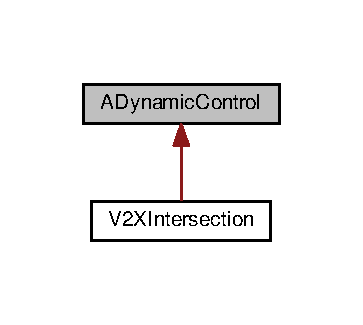
\includegraphics[width=174pt]{classADynamicControl__inherit__graph}
\end{center}
\end{figure}
\subsection*{Public Member Functions}
\begin{DoxyCompactItemize}
\item 
\hyperlink{classADynamicControl_a71b2b173a5b7ed4eb77a5c60fb5f1774}{A\+Dynamic\+Control} ()\hypertarget{classADynamicControl_a71b2b173a5b7ed4eb77a5c60fb5f1774}{}\label{classADynamicControl_a71b2b173a5b7ed4eb77a5c60fb5f1774}

\begin{DoxyCompactList}\small\item\em \hyperlink{classADynamicControl}{A\+Dynamic\+Control} Constructor. \end{DoxyCompactList}\item 
virtual \hyperlink{classADynamicControl_ac52fec4aa95f1cd9ec4d3c65c45f5233}{$\sim$\+A\+Dynamic\+Control} ()\hypertarget{classADynamicControl_ac52fec4aa95f1cd9ec4d3c65c45f5233}{}\label{classADynamicControl_ac52fec4aa95f1cd9ec4d3c65c45f5233}

\begin{DoxyCompactList}\small\item\em Deconstructor. \end{DoxyCompactList}\end{DoxyCompactItemize}


\subsection{Detailed Description}
The \hyperlink{classADynamicControl}{A\+Dynamic\+Control} class. 

Copyright T\+SS 2017

Author\+: Natale Patriciello \href{mailto:natale.patriciello@aimsun.com}{\tt natale.\+patriciello@aimsun.\+com} This is a placeholder and does not contain any code 

The documentation for this class was generated from the following file\+:\begin{DoxyCompactItemize}
\item 
include/core/\+A\+N\+G\+\_\+\+D\+T\+A/\+A\+Dynamic\+A\+P\+I/A\+Dynamic\+Control.\+h\end{DoxyCompactItemize}

\hypertarget{structAlacarteContainer}{}\section{Alacarte\+Container Struct Reference}
\label{structAlacarteContainer}\index{Alacarte\+Container@{Alacarte\+Container}}


Collaboration diagram for Alacarte\+Container\+:\nopagebreak
\begin{figure}[H]
\begin{center}
\leavevmode
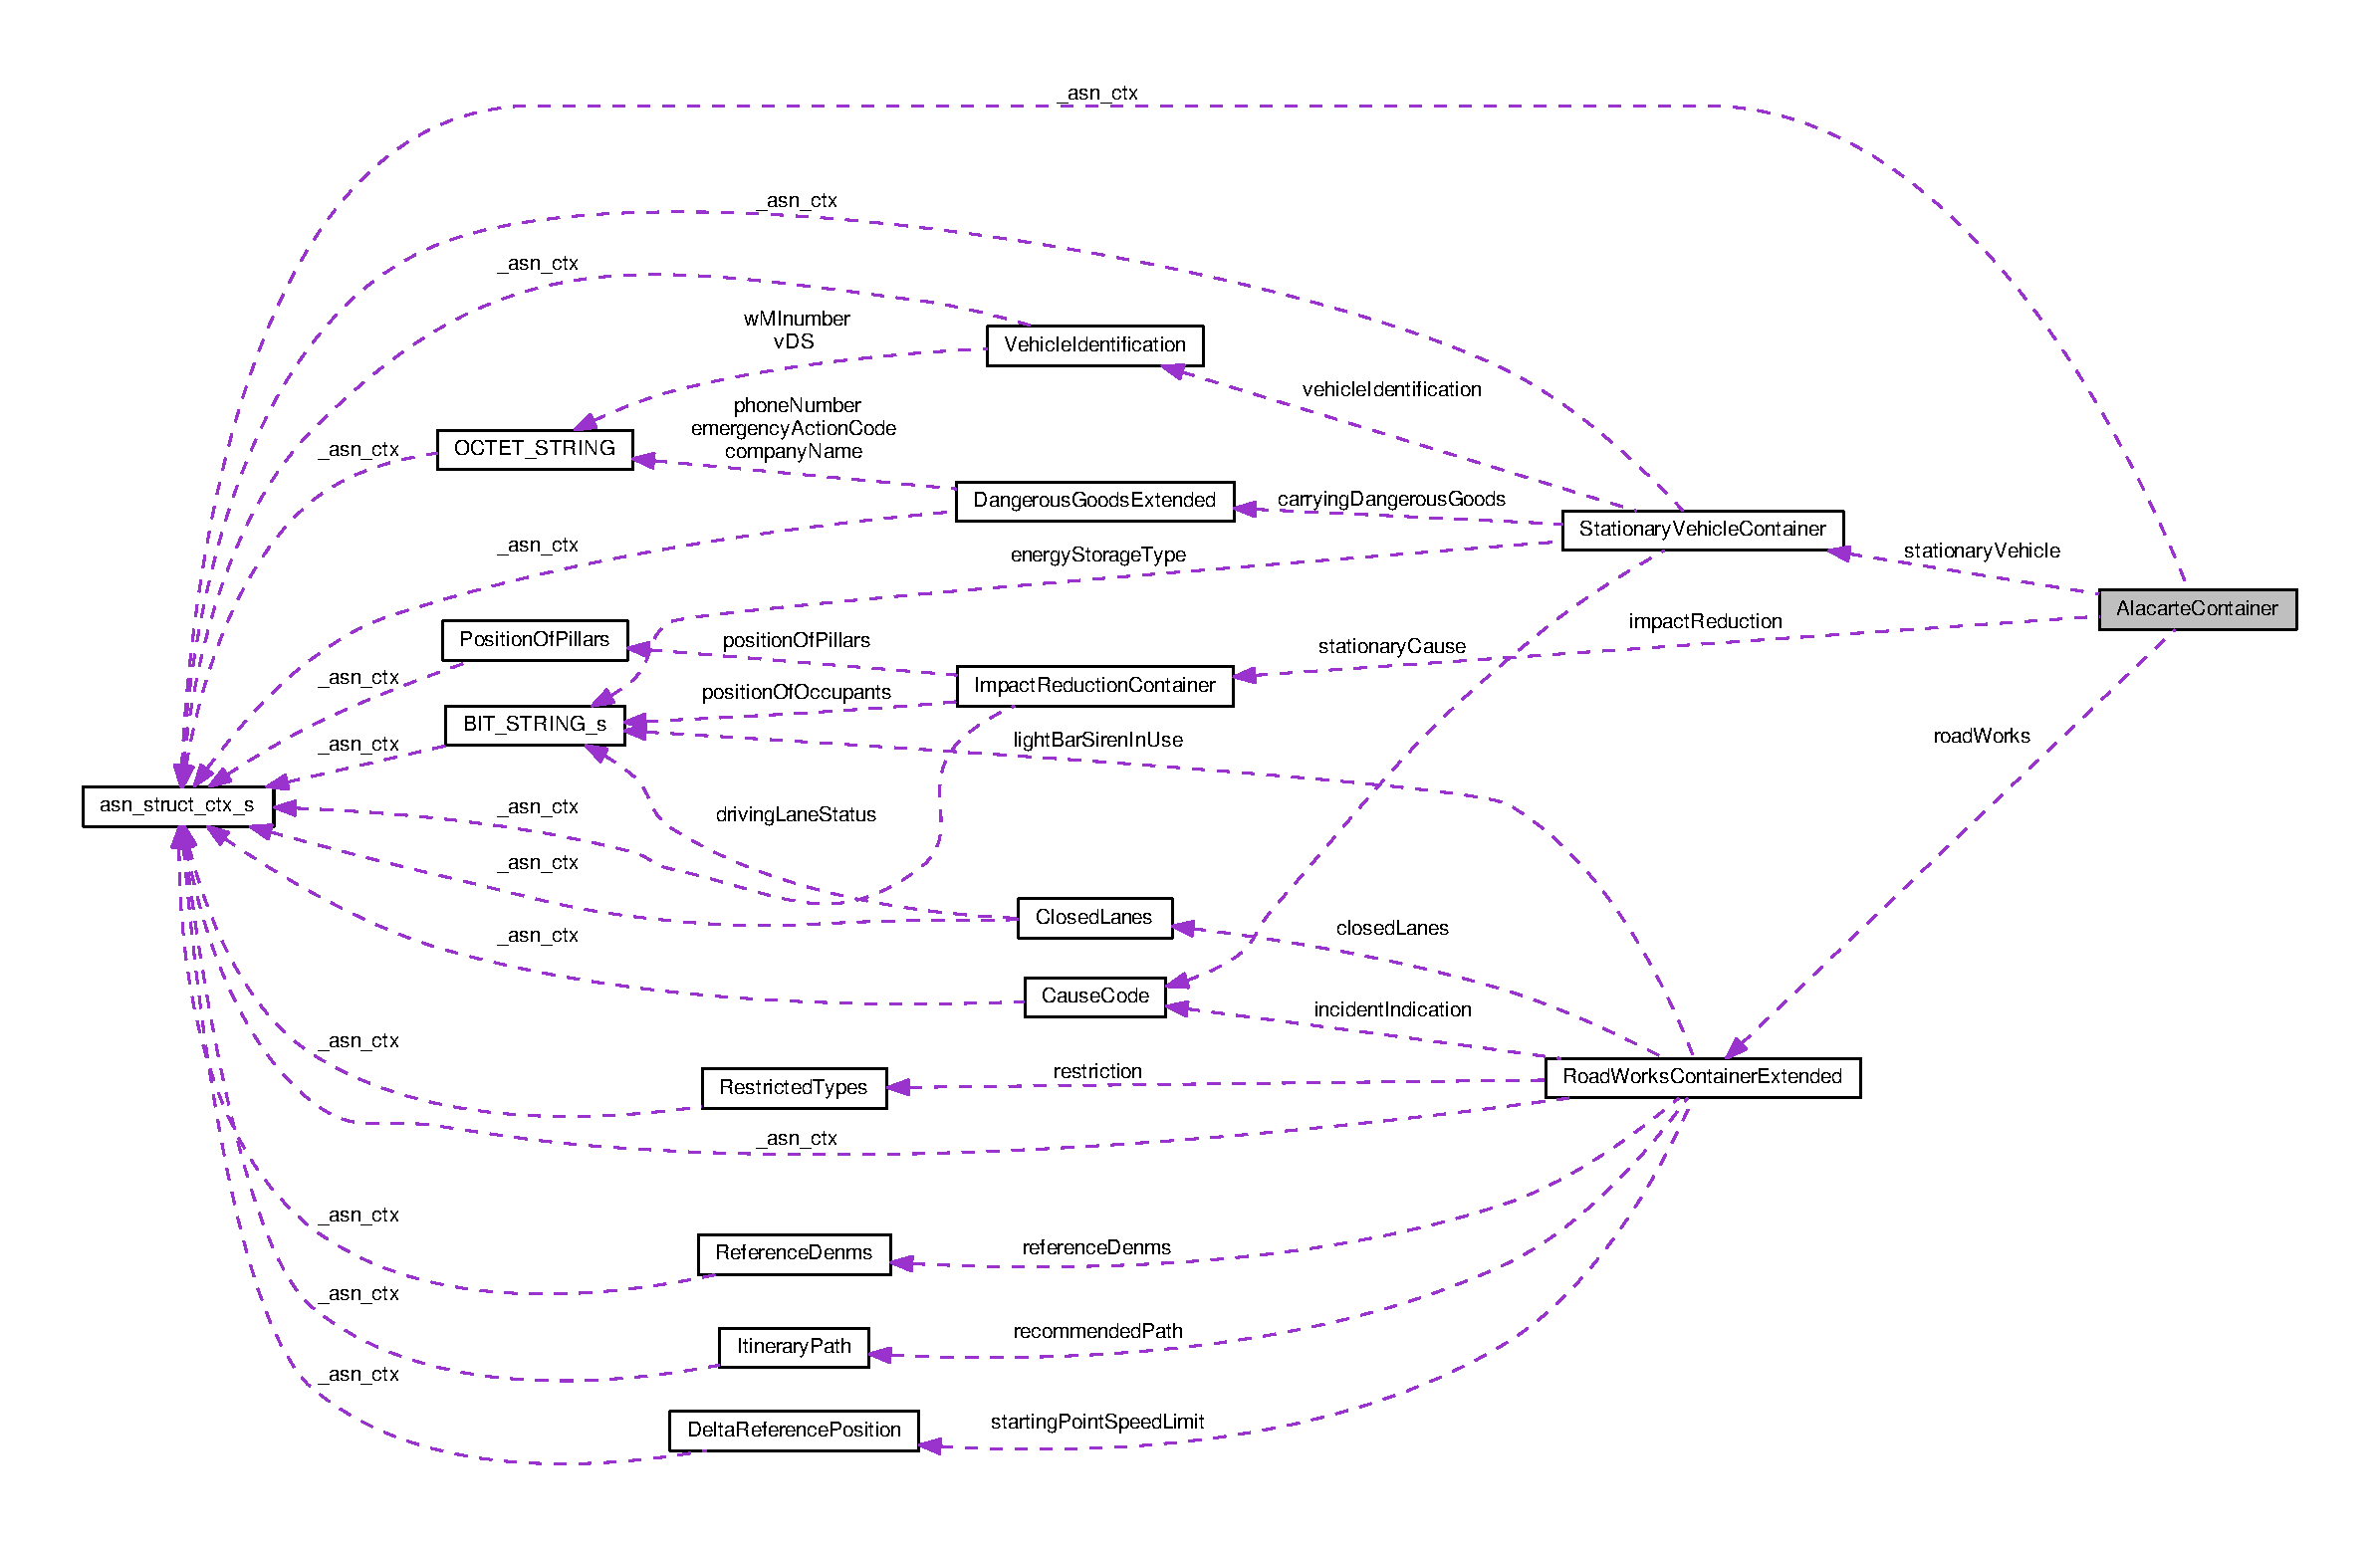
\includegraphics[width=350pt]{structAlacarteContainer__coll__graph}
\end{center}
\end{figure}
\subsection*{Public Attributes}
\begin{DoxyCompactItemize}
\item 
Lane\+Position\+\_\+t $\ast$ {\bfseries lane\+Position}\hypertarget{structAlacarteContainer_a820edd74451c678025808bff7c0e4d94}{}\label{structAlacarteContainer_a820edd74451c678025808bff7c0e4d94}

\item 
struct \hyperlink{structImpactReductionContainer}{Impact\+Reduction\+Container} $\ast$ {\bfseries impact\+Reduction}\hypertarget{structAlacarteContainer_aacb6e16622cf6a816ac9ed7bbd918fb4}{}\label{structAlacarteContainer_aacb6e16622cf6a816ac9ed7bbd918fb4}

\item 
Temperature\+\_\+t $\ast$ {\bfseries external\+Temperature}\hypertarget{structAlacarteContainer_ac653912d88f21766d79e87c961e816ca}{}\label{structAlacarteContainer_ac653912d88f21766d79e87c961e816ca}

\item 
struct \hyperlink{structRoadWorksContainerExtended}{Road\+Works\+Container\+Extended} $\ast$ {\bfseries road\+Works}\hypertarget{structAlacarteContainer_a3bf992f0424241519afc7b50638dc49b}{}\label{structAlacarteContainer_a3bf992f0424241519afc7b50638dc49b}

\item 
Positioning\+Solution\+Type\+\_\+t $\ast$ {\bfseries positioning\+Solution}\hypertarget{structAlacarteContainer_a6b14a10ec9d60bb2332f3f9bbee7ee76}{}\label{structAlacarteContainer_a6b14a10ec9d60bb2332f3f9bbee7ee76}

\item 
struct \hyperlink{structStationaryVehicleContainer}{Stationary\+Vehicle\+Container} $\ast$ {\bfseries stationary\+Vehicle}\hypertarget{structAlacarteContainer_abb3372826028718a5cebf71479af42a3}{}\label{structAlacarteContainer_abb3372826028718a5cebf71479af42a3}

\item 
\hyperlink{structasn__struct__ctx__s}{asn\+\_\+struct\+\_\+ctx\+\_\+t} {\bfseries \+\_\+asn\+\_\+ctx}\hypertarget{structAlacarteContainer_a983c4f09c51a878c0c6de982fc54b7db}{}\label{structAlacarteContainer_a983c4f09c51a878c0c6de982fc54b7db}

\end{DoxyCompactItemize}


The documentation for this struct was generated from the following file\+:\begin{DoxyCompactItemize}
\item 
include/aimsun\+\_\+extensions/\+V2\+X\+Framework/\+I\+T\+S-\/spec/Alacarte\+Container.\+h\end{DoxyCompactItemize}

\hypertarget{structAltitude}{}\section{Altitude Struct Reference}
\label{structAltitude}\index{Altitude@{Altitude}}


Collaboration diagram for Altitude\+:\nopagebreak
\begin{figure}[H]
\begin{center}
\leavevmode
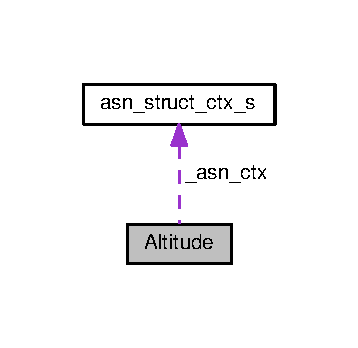
\includegraphics[width=172pt]{structAltitude__coll__graph}
\end{center}
\end{figure}
\subsection*{Public Attributes}
\begin{DoxyCompactItemize}
\item 
Altitude\+Value\+\_\+t {\bfseries altitude\+Value}\hypertarget{structAltitude_a1fec09d72cc65cfe51b1331bacc78ad4}{}\label{structAltitude_a1fec09d72cc65cfe51b1331bacc78ad4}

\item 
Altitude\+Confidence\+\_\+t {\bfseries altitude\+Confidence}\hypertarget{structAltitude_adb32cb3dd58733df3d926b5ee36e2c6e}{}\label{structAltitude_adb32cb3dd58733df3d926b5ee36e2c6e}

\item 
\hyperlink{structasn__struct__ctx__s}{asn\+\_\+struct\+\_\+ctx\+\_\+t} {\bfseries \+\_\+asn\+\_\+ctx}\hypertarget{structAltitude_af1f38d068dd9475657ab0f06bbadb781}{}\label{structAltitude_af1f38d068dd9475657ab0f06bbadb781}

\end{DoxyCompactItemize}


The documentation for this struct was generated from the following file\+:\begin{DoxyCompactItemize}
\item 
include/aimsun\+\_\+extensions/\+V2\+X\+Framework/\+I\+T\+S-\/spec/Altitude.\+h\end{DoxyCompactItemize}

\hypertarget{structANY}{}\section{A\+NY Struct Reference}
\label{structANY}\index{A\+NY@{A\+NY}}


Collaboration diagram for A\+NY\+:\nopagebreak
\begin{figure}[H]
\begin{center}
\leavevmode
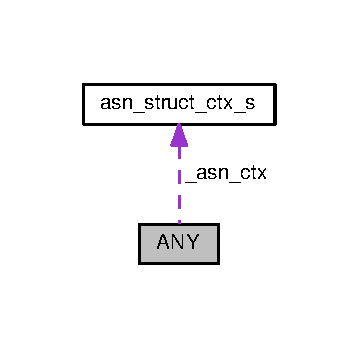
\includegraphics[width=172pt]{structANY__coll__graph}
\end{center}
\end{figure}
\subsection*{Public Attributes}
\begin{DoxyCompactItemize}
\item 
uint8\+\_\+t $\ast$ {\bfseries buf}\hypertarget{structANY_aa7fa72b14b21b2bf1a62b27b8a100c12}{}\label{structANY_aa7fa72b14b21b2bf1a62b27b8a100c12}

\item 
int {\bfseries size}\hypertarget{structANY_a0bdabe351f3c4ec465f659d3484e7b67}{}\label{structANY_a0bdabe351f3c4ec465f659d3484e7b67}

\item 
\hyperlink{structasn__struct__ctx__s}{asn\+\_\+struct\+\_\+ctx\+\_\+t} {\bfseries \+\_\+asn\+\_\+ctx}\hypertarget{structANY_a44c170a6a47e78a956a3aa748e869168}{}\label{structANY_a44c170a6a47e78a956a3aa748e869168}

\end{DoxyCompactItemize}


The documentation for this struct was generated from the following file\+:\begin{DoxyCompactItemize}
\item 
include/aimsun\+\_\+extensions/\+V2\+X\+Framework/\+A\+S\+N1/A\+N\+Y.\+h\end{DoxyCompactItemize}

\hypertarget{structAnyCatalogue}{}\section{Any\+Catalogue Struct Reference}
\label{structAnyCatalogue}\index{Any\+Catalogue@{Any\+Catalogue}}


Collaboration diagram for Any\+Catalogue\+:\nopagebreak
\begin{figure}[H]
\begin{center}
\leavevmode
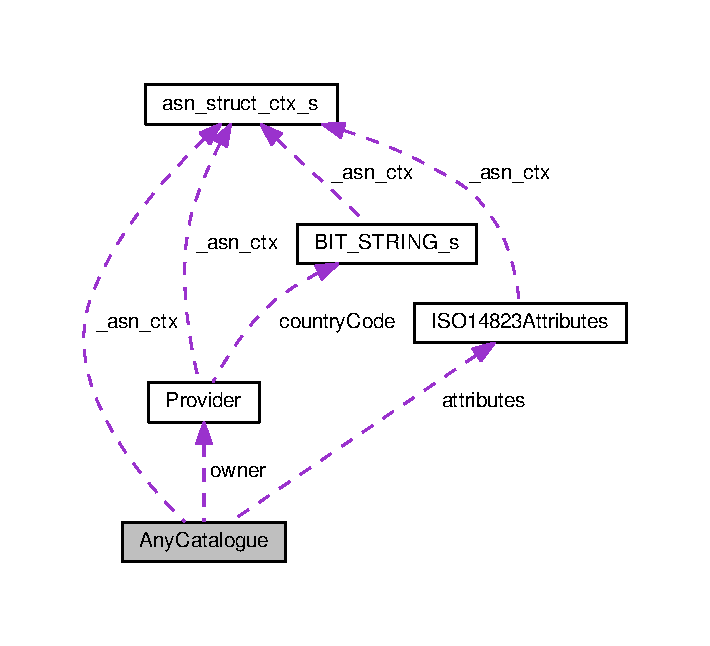
\includegraphics[width=341pt]{structAnyCatalogue__coll__graph}
\end{center}
\end{figure}
\subsection*{Public Attributes}
\begin{DoxyCompactItemize}
\item 
\hyperlink{structProvider}{Provider\+\_\+t} {\bfseries owner}\hypertarget{structAnyCatalogue_a36c2ae36127ce5857487f791a33f3af8}{}\label{structAnyCatalogue_a36c2ae36127ce5857487f791a33f3af8}

\item 
long {\bfseries version}\hypertarget{structAnyCatalogue_a2866ce802a7c4b128546f0e9c1ac910e}{}\label{structAnyCatalogue_a2866ce802a7c4b128546f0e9c1ac910e}

\item 
long {\bfseries pictogram\+Code}\hypertarget{structAnyCatalogue_afef8966d366612643de57aefcb0f1ae7}{}\label{structAnyCatalogue_afef8966d366612643de57aefcb0f1ae7}

\item 
long $\ast$ {\bfseries value}\hypertarget{structAnyCatalogue_a99e6fe7ad648a08204f2eb50ed4c827e}{}\label{structAnyCatalogue_a99e6fe7ad648a08204f2eb50ed4c827e}

\item 
R\+S\+C\+Unit\+\_\+t $\ast$ {\bfseries unit}\hypertarget{structAnyCatalogue_a31d2b8e236224d5c3da7c0acaede53a5}{}\label{structAnyCatalogue_a31d2b8e236224d5c3da7c0acaede53a5}

\item 
struct \hyperlink{structISO14823Attributes}{I\+S\+O14823\+Attributes} $\ast$ {\bfseries attributes}\hypertarget{structAnyCatalogue_aa95f29c9c142d3497c9122ebddf6bc3b}{}\label{structAnyCatalogue_aa95f29c9c142d3497c9122ebddf6bc3b}

\item 
\hyperlink{structasn__struct__ctx__s}{asn\+\_\+struct\+\_\+ctx\+\_\+t} {\bfseries \+\_\+asn\+\_\+ctx}\hypertarget{structAnyCatalogue_aa4be7c1871ae0e8abc516e1e762b8031}{}\label{structAnyCatalogue_aa4be7c1871ae0e8abc516e1e762b8031}

\end{DoxyCompactItemize}


The documentation for this struct was generated from the following file\+:\begin{DoxyCompactItemize}
\item 
include/aimsun\+\_\+extensions/\+V2\+X\+Framework/\+I\+T\+S-\/spec/Any\+Catalogue.\+h\end{DoxyCompactItemize}

\hypertarget{classARandomGenerator}{}\section{A\+Random\+Generator Class Reference}
\label{classARandomGenerator}\index{A\+Random\+Generator@{A\+Random\+Generator}}
\subsection*{Public Member Functions}
\begin{DoxyCompactItemize}
\item 
{\bfseries A\+Random\+Generator} (const \hyperlink{classARandomGenerator}{A\+Random\+Generator} \&other\+R\+NG)\hypertarget{classARandomGenerator_aa209ff80ec6623dd434c56e163597d8c}{}\label{classARandomGenerator_aa209ff80ec6623dd434c56e163597d8c}

\item 
{\bfseries A\+Random\+Generator} (int aseed)\hypertarget{classARandomGenerator_ab8a7945444c0aab6f4c61b1afa6e96a6}{}\label{classARandomGenerator_ab8a7945444c0aab6f4c61b1afa6e96a6}

\item 
\hyperlink{classARandomGenerator}{A\+Random\+Generator} \& {\bfseries operator=} (\hyperlink{classARandomGenerator}{A\+Random\+Generator} const \&other)\hypertarget{classARandomGenerator_a004e74cdd129366e21f9c9876096fd81}{}\label{classARandomGenerator_a004e74cdd129366e21f9c9876096fd81}

\item 
void {\bfseries set\+Seed} (int aseed)\hypertarget{classARandomGenerator_a82e7f7c641f4bd4caa4e43db2f32468a}{}\label{classARandomGenerator_a82e7f7c641f4bd4caa4e43db2f32468a}

\item 
int {\bfseries get\+Seed} () const \hypertarget{classARandomGenerator_a11d8618fbf6539f2b4f0d919a5dad9a7}{}\label{classARandomGenerator_a11d8618fbf6539f2b4f0d919a5dad9a7}

\item 
int $\ast$ {\bfseries get\+Ref\+Seed} ()\hypertarget{classARandomGenerator_a7764d336630fdb25f8219d29e2d9ae80}{}\label{classARandomGenerator_a7764d336630fdb25f8219d29e2d9ae80}

\item 
virtual double {\bfseries random01} ()\hypertarget{classARandomGenerator_a7bed33db3faf4b39fa08eee18782ecb1}{}\label{classARandomGenerator_a7bed33db3faf4b39fa08eee18782ecb1}

\item 
double {\bfseries uniform} (double a, double b)\hypertarget{classARandomGenerator_a69017d79b869ef608affa8b82b1e607e}{}\label{classARandomGenerator_a69017d79b869ef608affa8b82b1e607e}

\item 
double {\bfseries normal} (double mu, double sigma)\hypertarget{classARandomGenerator_aec025a2421d67fded97e85ef6f7a2fca}{}\label{classARandomGenerator_aec025a2421d67fded97e85ef6f7a2fca}

\item 
double {\bfseries normalfull} (double mu, double sigma)\hypertarget{classARandomGenerator_acbef92da4df9b3c8de59341b71611440}{}\label{classARandomGenerator_acbef92da4df9b3c8de59341b71611440}

\item 
double \hyperlink{classARandomGenerator_a85e2f9a6b4c39d19c4bc4beadfa9dbfb}{normal\+\_\+mt} (double mu, double sigma, double amin, double amax, double $\ast$first\+Random\+Num=N\+U\+LL, double $\ast$second\+Random\+Num=N\+U\+LL)
\item 
double {\bfseries lognormal\+\_\+mt} (double mu, double sigma, double min, double max)\hypertarget{classARandomGenerator_aaad820ff562ed1242caa0de2baa1f51c}{}\label{classARandomGenerator_aaad820ff562ed1242caa0de2baa1f51c}

\item 
double {\bfseries exponential} (double lambda)\hypertarget{classARandomGenerator_a8b2d07c0d5523187adf4aa2e3f5b6670}{}\label{classARandomGenerator_a8b2d07c0d5523187adf4aa2e3f5b6670}

\item 
double {\bfseries get\+Headway} (int headway\+Type, double time\+Between\+Vehs, double shiftfactor)\hypertarget{classARandomGenerator_a495b02983cb88cd90de855296258fa8b}{}\label{classARandomGenerator_a495b02983cb88cd90de855296258fa8b}

\item 
int {\bfseries random\+Class} (int n)\hypertarget{classARandomGenerator_a1ab5c007ca0d56262c774f5c311f28b3}{}\label{classARandomGenerator_a1ab5c007ca0d56262c774f5c311f28b3}

\item 
int {\bfseries get\+New\+Seed} ()\hypertarget{classARandomGenerator_adf4750f97d3ae800643c7d8d61ffbf45}{}\label{classARandomGenerator_adf4750f97d3ae800643c7d8d61ffbf45}

\item 
void {\bfseries store\+State} (Q\+Data\+Stream \&stream)\hypertarget{classARandomGenerator_a6cfbac4a9b0aabd8b09ffbd7627202d2}{}\label{classARandomGenerator_a6cfbac4a9b0aabd8b09ffbd7627202d2}

\item 
void {\bfseries restore\+State} (Q\+Data\+Stream \&stream)\hypertarget{classARandomGenerator_a557b66ccbc65a2513c327b070ec74154}{}\label{classARandomGenerator_a557b66ccbc65a2513c327b070ec74154}

\end{DoxyCompactItemize}
\subsection*{Static Public Member Functions}
\begin{DoxyCompactItemize}
\item 
static double {\bfseries uniform} (double value01, double a, double b)\hypertarget{classARandomGenerator_a5d718b7a952f71e3741b4d3d75ec2413}{}\label{classARandomGenerator_a5d718b7a952f71e3741b4d3d75ec2413}

\end{DoxyCompactItemize}
\subsection*{Protected Attributes}
\begin{DoxyCompactItemize}
\item 
int {\bfseries seed}\hypertarget{classARandomGenerator_a7b7d03496867576ed46b39ca3ce10236}{}\label{classARandomGenerator_a7b7d03496867576ed46b39ca3ce10236}

\end{DoxyCompactItemize}


\subsection{Member Function Documentation}
\index{A\+Random\+Generator@{A\+Random\+Generator}!normal\+\_\+mt@{normal\+\_\+mt}}
\index{normal\+\_\+mt@{normal\+\_\+mt}!A\+Random\+Generator@{A\+Random\+Generator}}
\subsubsection[{\texorpdfstring{normal\+\_\+mt(double mu, double sigma, double amin, double amax, double $\ast$first\+Random\+Num=\+N\+U\+L\+L, double $\ast$second\+Random\+Num=\+N\+U\+L\+L)}{normal_mt(double mu, double sigma, double amin, double amax, double *firstRandomNum=NULL, double *secondRandomNum=NULL)}}]{\setlength{\rightskip}{0pt plus 5cm}double A\+Random\+Generator\+::normal\+\_\+mt (
\begin{DoxyParamCaption}
\item[{double}]{mu, }
\item[{double}]{sigma, }
\item[{double}]{amin, }
\item[{double}]{amax, }
\item[{double $\ast$}]{first\+Random\+Num = {\ttfamily NULL}, }
\item[{double $\ast$}]{second\+Random\+Num = {\ttfamily NULL}}
\end{DoxyParamCaption}
)}\hypertarget{classARandomGenerator_a85e2f9a6b4c39d19c4bc4beadfa9dbfb}{}\label{classARandomGenerator_a85e2f9a6b4c39d19c4bc4beadfa9dbfb}
first\+Random\+Num and second\+Random\+Num can be externally specified and also returned. When they are not null and their value is $>$ 0 they will be used instead of generating them using the random01() function. If they are not null, the random numbers used will be returned. 

The documentation for this class was generated from the following file\+:\begin{DoxyCompactItemize}
\item 
include/core/random/F\+Rand.\+h\end{DoxyCompactItemize}

\hypertarget{classASN1CContainer}{}\section{A\+S\+N1\+C\+Container$<$ asn\+\_\+\+T\+Y\+PE $>$ Class Template Reference}
\label{classASN1CContainer}\index{A\+S\+N1\+C\+Container$<$ asn\+\_\+\+T\+Y\+P\+E $>$@{A\+S\+N1\+C\+Container$<$ asn\+\_\+\+T\+Y\+P\+E $>$}}


Container class for a type generated by asn.\+1 C compiler (\href{https://lionet.info/asn1c/blog/}{\tt https\+://lionet.\+info/asn1c/blog/})  




{\ttfamily \#include $<$Asn1c\+Container.\+h$>$}



Inheritance diagram for A\+S\+N1\+C\+Container$<$ asn\+\_\+\+T\+Y\+PE $>$\+:\nopagebreak
\begin{figure}[H]
\begin{center}
\leavevmode
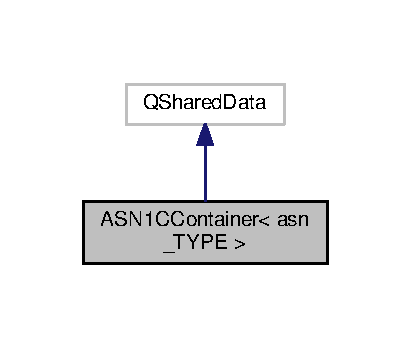
\includegraphics[width=197pt]{classASN1CContainer__inherit__graph}
\end{center}
\end{figure}


Collaboration diagram for A\+S\+N1\+C\+Container$<$ asn\+\_\+\+T\+Y\+PE $>$\+:\nopagebreak
\begin{figure}[H]
\begin{center}
\leavevmode
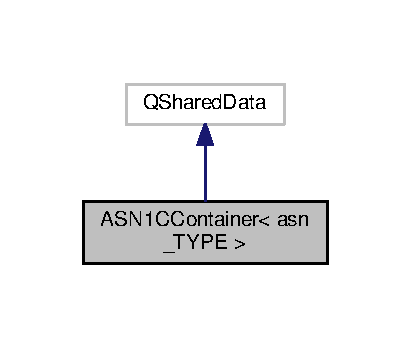
\includegraphics[width=197pt]{classASN1CContainer__coll__graph}
\end{center}
\end{figure}
\subsection*{Public Member Functions}
\begin{DoxyCompactItemize}
\item 
\hyperlink{classASN1CContainer_ad8d69cd8ce21023ea36410113162a008}{A\+S\+N1\+C\+Container} ()
\begin{DoxyCompactList}\small\item\em Creating an empty (and invalid) \hyperlink{classASN1CContainer}{A\+S\+N1\+C\+Container}. \end{DoxyCompactList}\item 
\hyperlink{classASN1CContainer_a0fdf5aaaef51b6b9c1e10442e6e72890}{A\+S\+N1\+C\+Container} (const \hyperlink{classASN1CContainer}{A\+S\+N1\+C\+Container} \&other)
\begin{DoxyCompactList}\small\item\em Copy another object (deep copy) \end{DoxyCompactList}\item 
\hyperlink{classASN1CContainer_a26020bb451f75d62ae28bc43568aee17}{$\sim$\+A\+S\+N1\+C\+Container} ()
\begin{DoxyCompactList}\small\item\em Deconstructor. \end{DoxyCompactList}\item 
asn\+\_\+\+T\+Y\+PE $\ast$ \hyperlink{classASN1CContainer_a025329e80ae2a3216fc1d1cf6a8f957d}{data} ()
\begin{DoxyCompactList}\small\item\em Return a pointer to the A\+S\+N.\+1 structure, allowing reading and editing. \end{DoxyCompactList}\item 
asn\+\_\+\+T\+Y\+PE const $\ast$ \hyperlink{classASN1CContainer_a7db5e6ea01cfc7dc209b73788a034b81}{const\+Data} () const 
\begin{DoxyCompactList}\small\item\em Return a const pointer to the A\+S\+N.\+1 structure, allowing reading. \end{DoxyCompactList}\item 
void \hyperlink{classASN1CContainer_a7c7691789087f204c37207590eaaf89d}{initialize\+Empty} ()\hypertarget{classASN1CContainer_a7c7691789087f204c37207590eaaf89d}{}\label{classASN1CContainer_a7c7691789087f204c37207590eaaf89d}

\begin{DoxyCompactList}\small\item\em Allocate the memory for a manual editing of the message. \end{DoxyCompactList}\item 
bool \hyperlink{classASN1CContainer_a67a086c665ecbf7a54e390c8fb7df47f}{has\+Data} () const 
\begin{DoxyCompactList}\small\item\em Check if the underlying data is valid. \end{DoxyCompactList}\item 
void \hyperlink{classASN1CContainer_a61559655caab168362a30c0538950ba3}{set\+Type\+Def} (\hyperlink{structasn__TYPE__descriptor__s}{asn\+\_\+\+T\+Y\+P\+E\+\_\+descriptor\+\_\+s} $\ast$asn\+Def)
\begin{DoxyCompactList}\small\item\em Set the type definition. \end{DoxyCompactList}\item 
void \hyperlink{classASN1CContainer_a6492cd5793ca9e2ab073445b358a68b5}{clear} ()
\begin{DoxyCompactList}\small\item\em Perform all the required operation to clear the memory. \end{DoxyCompactList}\item 
bool \hyperlink{classASN1CContainer_ae444a9554d1a856d74a942f70a3b2fb8}{to\+X\+ML} (std\+::ostream $\ast$output) const 
\begin{DoxyCompactList}\small\item\em Write the data structure to a X\+ML output. \end{DoxyCompactList}\item 
bool \hyperlink{classASN1CContainer_a165c57c9a77d80d5f8cd6c2d6b902650}{to\+X\+ML} (const char $\ast$filename) const 
\begin{DoxyCompactList}\small\item\em Write the data structure to a X\+ML file. \end{DoxyCompactList}\item 
bool \hyperlink{classASN1CContainer_af84be317f31518978a63621b4fc67c40}{to\+D\+ER} (std\+::vector$<$ char $>$ $\ast$output) const 
\begin{DoxyCompactList}\small\item\em Write the data structure to a binary output. \end{DoxyCompactList}\item 
bool \hyperlink{classASN1CContainer_ae3fa0fbad6b0375b36a73be41f2e8075}{to\+D\+ER} (const char $\ast$filename) const 
\begin{DoxyCompactList}\small\item\em Write the data structure to a binary file. \end{DoxyCompactList}\item 
bool \hyperlink{classASN1CContainer_aac98fb872b823dfaffce36a8bf24ddbe}{from\+X\+ML} (const char $\ast$buf, size\+\_\+t size)
\begin{DoxyCompactList}\small\item\em Read the data structure from X\+ML input. \end{DoxyCompactList}\item 
bool \hyperlink{classASN1CContainer_af43531162a367d3b79be39e90ec72ebb}{from\+X\+ML} (const char $\ast$filename)
\begin{DoxyCompactList}\small\item\em Read the data structure from an X\+ML file. \end{DoxyCompactList}\item 
bool \hyperlink{classASN1CContainer_a08fc60e1d78b99b33a19dba1f1c39900}{from\+B\+ER} (const char $\ast$buf, size\+\_\+t size)
\begin{DoxyCompactList}\small\item\em Read the data structure from binary input. \end{DoxyCompactList}\item 
bool \hyperlink{classASN1CContainer_afbeda1aa393679759574f17e34cedf06}{from\+B\+ER} (const std\+::vector$<$ char $>$ \&input)
\begin{DoxyCompactList}\small\item\em Read the data structure from binary input. \end{DoxyCompactList}\item 
bool \hyperlink{classASN1CContainer_a7465eb755c1031b3745796faa02781ad}{from\+B\+ER} (const char $\ast$filename)
\begin{DoxyCompactList}\small\item\em Read the data structure from a binary file. \end{DoxyCompactList}\item 
void \hyperlink{classASN1CContainer_acc5d252d15af64426472504f04f2b1e8}{to\+Console} () const \hypertarget{classASN1CContainer_acc5d252d15af64426472504f04f2b1e8}{}\label{classASN1CContainer_acc5d252d15af64426472504f04f2b1e8}

\begin{DoxyCompactList}\small\item\em Print the data to std\+::cout. \end{DoxyCompactList}\end{DoxyCompactItemize}
\subsection*{Protected Types}
\begin{DoxyCompactItemize}
\item 
typedef \hyperlink{structasn__dec__rval__s}{asn\+\_\+dec\+\_\+rval\+\_\+t}($\ast$ \hyperlink{classASN1CContainer_a9edaf11eed4f5ded9a32200e43832e72}{asn\+\_\+decode}) (struct \hyperlink{structasn__codec__ctx__s}{asn\+\_\+codec\+\_\+ctx\+\_\+s} $\ast$, struct \hyperlink{structasn__TYPE__descriptor__s}{asn\+\_\+\+T\+Y\+P\+E\+\_\+descriptor\+\_\+s} $\ast$, void $\ast$$\ast$, const void $\ast$, size\+\_\+t)\hypertarget{classASN1CContainer_a9edaf11eed4f5ded9a32200e43832e72}{}\label{classASN1CContainer_a9edaf11eed4f5ded9a32200e43832e72}

\begin{DoxyCompactList}\small\item\em Define a type for the decode functions provided by the C compiler. \end{DoxyCompactList}\item 
typedef bool(\hyperlink{classASN1CContainer}{A\+S\+N1\+C\+Container}$<$ asn\+\_\+\+T\+Y\+PE $>$\+::$\ast$ \hyperlink{classASN1CContainer_a5830db096eef3cee08cb7e948624aa3c}{from\+Fn}) (const char $\ast$buf, size\+\_\+t size)\hypertarget{classASN1CContainer_a5830db096eef3cee08cb7e948624aa3c}{}\label{classASN1CContainer_a5830db096eef3cee08cb7e948624aa3c}

\begin{DoxyCompactList}\small\item\em Define a type from the various from$\ast$ function defined in this class. \end{DoxyCompactList}\end{DoxyCompactItemize}
\subsection*{Protected Member Functions}
\begin{DoxyCompactItemize}
\item 
void \hyperlink{classASN1CContainer_aca77386df5f80660d8a72481d96eabe0}{set\+Data} (asn\+\_\+\+T\+Y\+PE $\ast$\hyperlink{classASN1CContainer_a025329e80ae2a3216fc1d1cf6a8f957d}{data})
\begin{DoxyCompactList}\small\item\em Set the underlying data of this object. \end{DoxyCompactList}\item 
bool \hyperlink{classASN1CContainer_a24949d778b5d738c17f80127ab4b188f}{from\+Buf} (const char $\ast$buf, size\+\_\+t size, \hyperlink{classASN1CContainer_a9edaf11eed4f5ded9a32200e43832e72}{asn\+\_\+decode} decode)
\begin{DoxyCompactList}\small\item\em Read the data from a buffer, using the a specified function for decoding. \end{DoxyCompactList}\item 
bool \hyperlink{classASN1CContainer_a90a2a5fbe0601dff3b2ac886f06afd6b}{from\+File} (const char $\ast$filename, \hyperlink{classASN1CContainer_a5830db096eef3cee08cb7e948624aa3c}{from\+Fn} function)
\begin{DoxyCompactList}\small\item\em Read the data from a file, using the a specified function for decoding. \end{DoxyCompactList}\item 
bool \hyperlink{classASN1CContainer_a6fec3867e5aa5893dc497add7f179111}{to\+File} (const char $\ast$filename) const 
\begin{DoxyCompactList}\small\item\em Write the data to a file. \end{DoxyCompactList}\end{DoxyCompactItemize}
\subsection*{Static Protected Member Functions}
\begin{DoxyCompactItemize}
\item 
static int \hyperlink{classASN1CContainer_aa0216c3146bad94b0429fd56da4565f0}{write\+Buf\+To\+Ofstream} (const void $\ast$buffer, size\+\_\+t size, void $\ast$app\+\_\+key)
\begin{DoxyCompactList}\small\item\em Write a buffer to output stream. \end{DoxyCompactList}\item 
static int \hyperlink{classASN1CContainer_a89eaae98d4b34890bc8745bf0f834c8d}{write\+Buf\+To\+Vector} (const void $\ast$buffer, size\+\_\+t size, void $\ast$app\+\_\+key)
\begin{DoxyCompactList}\small\item\em Write a buffer to output vector. \end{DoxyCompactList}\end{DoxyCompactItemize}


\subsection{Detailed Description}
\subsubsection*{template$<$typename asn\+\_\+\+T\+Y\+PE$>$\\*
class A\+S\+N1\+C\+Container$<$ asn\+\_\+\+T\+Y\+P\+E $>$}

Container class for a type generated by asn.\+1 C compiler (\href{https://lionet.info/asn1c/blog/}{\tt https\+://lionet.\+info/asn1c/blog/}) 

{\bfseries  What is A\+S\+N.\+1? }

A\+S\+N.\+1 stands for Abstract Syntax Notation One. It allows describing complex data structures independently of any particular programming language. The A\+S\+N.\+1 compiler would take these A\+S\+N.\+1 specifications and produce a set of target language (C, C++, Java) files which would contain the native type definitions for these abstractly specified structures, and also generate a code which would perform the conversions of these structures into/from a series of bytes (serialization/deserialization), (presumably, these routines would be useful if the structure is going to be transferred over the network or written to an external media).

There are multiple data encodings developed for A\+S\+N.\+1. The most widely used ones are B\+ER (Basic Encoding Rules), C\+ER (Canonical-\/), D\+ER (Distinguished Encoding Rules), P\+ER (Packed Encoding Rules) and X\+ER (X\+ML Encoding Rules).

{\bfseries  How Aimsun deal with A\+S\+N.\+1 }

In Aimsun we make use of the B\+SD asn.\+1 C compiler to translate the A\+S\+N.\+1 specification into C++-\/compatible data structures. \hyperlink{classASN1CContainer}{A\+S\+N1\+C\+Container} was born to hide the C-\/functions and structures that follow from this process. This container can be used in junction with Q\+Shared\+Data\+Pointer to implement a Copy-\/\+On-\/\+Write semantic. This class is not meant to be used without a container which abstracts the functionalities provided in the following because these can change in future (we can\textquotesingle{}t predict if the output of the asn.\+1 C compiler will be the same in the future).

For an example of usage, please look to the class \hyperlink{classCAMMessage}{C\+A\+M\+Message}. It is necessary to initialize the class by setting the type definition created by the A\+S\+N.\+1 compiler (set\+Type\+Def), and if a manual modification to the internal data is needed, it is necessary to call the method initialize\+Empty to allocate the internal memory; is not possible to do this initialization in the constructor due to a lack of a custom constructor in the Q\+Shared\+Data\+Pointer class.

{\bfseries  How to write a class which uses a type derived from the A\+S\+N.\+1 compiler }

Let\textquotesingle{}s start with a simple A\+S\+N.\+1 definition\+:


\begin{DoxyCode}
1 MyModule DEFINITIONS ::=
2 BEGIN
3 
4 MyTypes ::= SEQUENCE \{
5   myObjectId OBJECT IDENTIFIER,
6   mySeqOf SEQUENCE OF MyInt,
7   myBitString BIT STRING \{
8                     muxToken(0),
9                     modemToken(1)
10               \}
11 \}
12 
13 MyInt ::= INTEGER (0..65535) END
\end{DoxyCode}


Compiling this definition will generate a lot of files; however, the main type will be a struct My\+Types\+\_\+t. This type is mean to be enclosed in the class \hyperlink{classASN1CContainer}{A\+S\+N1\+C\+Container}\+: 
\begin{DoxyCode}
...
private:
    QSharedDataPointer< ASN1CContainer<MyTypes\_t> > m\_message;
...
\end{DoxyCode}


Let\textquotesingle{}s suppose that the shared pointer m\+\_\+message is a private member of the class called My\+Type\+Message. It is recommended to initialize the variable in the constructors\+: 
\begin{DoxyCode}
\textcolor{preprocessor}{#include "MyTypes.h"} \textcolor{comment}{// Generated by the asn.1 compiler}

MyTypeMessage::MyTypeMessage()
\{
    m\_message = \textcolor{keyword}{new} \hyperlink{classASN1CContainer}{ASN1CContainer<MyTypes\_t>} ();
    m\_message->\hyperlink{classASN1CContainer_a61559655caab168362a30c0538950ba3}{setTypeDef}(&asn\_DEF\_MyTypes);
\}
\end{DoxyCode}
 The object asn\+\_\+\+D\+E\+F\+\_\+\+My\+Types is created automatically by the asn.\+1 compiler, and defined in the main header of the generated files. It is strictly necessary to set the type definition, or the other methods (including the deconstructor and the memory management) will not work.

Giving the C\+OW characteristic of the class, in the deconstructor is not possible to delete the class. The object will be automatically deleted when the internal reference count reaches 0; destroying the pointer, done automatically in the My\+Type\+Message deconstructor, decrements the reference count. 
\begin{DoxyCode}
MyTypeMessage::~MyTypeMessage()
\{
    \textcolor{comment}{// Do not delete m\_message;}
\}
\end{DoxyCode}


The message can now be automatically built from an X\+ML file, a byte stream, or a byte file through the corresponding from$\ast$ functions. For instance\+: 
\begin{DoxyCode}
\textcolor{keywordtype}{bool} MyTypeMessage::FromXML(\textcolor{keyword}{const} \textcolor{keywordtype}{char} *filename)
\{
    \textcolor{keywordflow}{return} m\_message->fromXML(filename);
\}
\end{DoxyCode}


To access the data in a read-\/only way, it is possible to provide to the user a const access to the data contained in the message itself. For writing access, it is possible to provide a non-\/const access. Please note that any non-\/const access to the data, if the reference count of the object is greater than 1, will trigger a deep object copy.


\begin{DoxyCode}
\textcolor{keyword}{const} MyTypes\_t* MyTypeMessage::constData()\textcolor{keyword}{ const}
\textcolor{keyword}{}\{
   \textcolor{keywordflow}{return} m\_message.constData()->constData();
\}

MyTypes\_t* MyTypeMessage::data()
\{
   \textcolor{keywordflow}{return} m\_message.data()->data();
\}
\end{DoxyCode}
 

\subsection{Constructor \& Destructor Documentation}
\index{A\+S\+N1\+C\+Container@{A\+S\+N1\+C\+Container}!A\+S\+N1\+C\+Container@{A\+S\+N1\+C\+Container}}
\index{A\+S\+N1\+C\+Container@{A\+S\+N1\+C\+Container}!A\+S\+N1\+C\+Container@{A\+S\+N1\+C\+Container}}
\subsubsection[{\texorpdfstring{A\+S\+N1\+C\+Container()}{ASN1CContainer()}}]{\setlength{\rightskip}{0pt plus 5cm}template$<$typename asn\+\_\+\+T\+Y\+PE $>$ {\bf A\+S\+N1\+C\+Container}$<$ asn\+\_\+\+T\+Y\+PE $>$\+::{\bf A\+S\+N1\+C\+Container} (
\begin{DoxyParamCaption}
{}
\end{DoxyParamCaption}
)}\hypertarget{classASN1CContainer_ad8d69cd8ce21023ea36410113162a008}{}\label{classASN1CContainer_ad8d69cd8ce21023ea36410113162a008}


Creating an empty (and invalid) \hyperlink{classASN1CContainer}{A\+S\+N1\+C\+Container}. 

To validate the object, call set\+Type\+Def. \index{A\+S\+N1\+C\+Container@{A\+S\+N1\+C\+Container}!A\+S\+N1\+C\+Container@{A\+S\+N1\+C\+Container}}
\index{A\+S\+N1\+C\+Container@{A\+S\+N1\+C\+Container}!A\+S\+N1\+C\+Container@{A\+S\+N1\+C\+Container}}
\subsubsection[{\texorpdfstring{A\+S\+N1\+C\+Container(const A\+S\+N1\+C\+Container \&other)}{ASN1CContainer(const ASN1CContainer &other)}}]{\setlength{\rightskip}{0pt plus 5cm}template$<$typename asn\+\_\+\+T\+Y\+PE $>$ {\bf A\+S\+N1\+C\+Container}$<$ asn\+\_\+\+T\+Y\+PE $>$\+::{\bf A\+S\+N1\+C\+Container} (
\begin{DoxyParamCaption}
\item[{const {\bf A\+S\+N1\+C\+Container}$<$ asn\+\_\+\+T\+Y\+PE $>$ \&}]{other}
\end{DoxyParamCaption}
)}\hypertarget{classASN1CContainer_a0fdf5aaaef51b6b9c1e10442e6e72890}{}\label{classASN1CContainer_a0fdf5aaaef51b6b9c1e10442e6e72890}


Copy another object (deep copy) 


\begin{DoxyParams}{Parameters}
{\em other} & other object \\
\hline
\end{DoxyParams}
\index{A\+S\+N1\+C\+Container@{A\+S\+N1\+C\+Container}!````~A\+S\+N1\+C\+Container@{$\sim$\+A\+S\+N1\+C\+Container}}
\index{````~A\+S\+N1\+C\+Container@{$\sim$\+A\+S\+N1\+C\+Container}!A\+S\+N1\+C\+Container@{A\+S\+N1\+C\+Container}}
\subsubsection[{\texorpdfstring{$\sim$\+A\+S\+N1\+C\+Container()}{~ASN1CContainer()}}]{\setlength{\rightskip}{0pt plus 5cm}template$<$typename asn\+\_\+\+T\+Y\+PE $>$ {\bf A\+S\+N1\+C\+Container}$<$ asn\+\_\+\+T\+Y\+PE $>$\+::$\sim${\bf A\+S\+N1\+C\+Container} (
\begin{DoxyParamCaption}
{}
\end{DoxyParamCaption}
)}\hypertarget{classASN1CContainer_a26020bb451f75d62ae28bc43568aee17}{}\label{classASN1CContainer_a26020bb451f75d62ae28bc43568aee17}


Deconstructor. 

It calls \hyperlink{classASN1CContainer_a6492cd5793ca9e2ab073445b358a68b5}{clear()} to perform all the required delete operations. 

\subsection{Member Function Documentation}
\index{A\+S\+N1\+C\+Container@{A\+S\+N1\+C\+Container}!clear@{clear}}
\index{clear@{clear}!A\+S\+N1\+C\+Container@{A\+S\+N1\+C\+Container}}
\subsubsection[{\texorpdfstring{clear()}{clear()}}]{\setlength{\rightskip}{0pt plus 5cm}template$<$typename asn\+\_\+\+T\+Y\+PE $>$ void {\bf A\+S\+N1\+C\+Container}$<$ asn\+\_\+\+T\+Y\+PE $>$\+::clear (
\begin{DoxyParamCaption}
{}
\end{DoxyParamCaption}
)}\hypertarget{classASN1CContainer_a6492cd5793ca9e2ab073445b358a68b5}{}\label{classASN1CContainer_a6492cd5793ca9e2ab073445b358a68b5}


Perform all the required operation to clear the memory. 

This actually delete the underlying data structure. \index{A\+S\+N1\+C\+Container@{A\+S\+N1\+C\+Container}!const\+Data@{const\+Data}}
\index{const\+Data@{const\+Data}!A\+S\+N1\+C\+Container@{A\+S\+N1\+C\+Container}}
\subsubsection[{\texorpdfstring{const\+Data() const }{constData() const }}]{\setlength{\rightskip}{0pt plus 5cm}template$<$typename asn\+\_\+\+T\+Y\+PE $>$ asn\+\_\+\+T\+Y\+PE const $\ast$ {\bf A\+S\+N1\+C\+Container}$<$ asn\+\_\+\+T\+Y\+PE $>$\+::const\+Data (
\begin{DoxyParamCaption}
{}
\end{DoxyParamCaption}
) const}\hypertarget{classASN1CContainer_a7db5e6ea01cfc7dc209b73788a034b81}{}\label{classASN1CContainer_a7db5e6ea01cfc7dc209b73788a034b81}


Return a const pointer to the A\+S\+N.\+1 structure, allowing reading. 

It is not possible to edit the structure, thus no deep copy will be triggered.

\begin{DoxyReturn}{Returns}
Pointer to the generated A\+S\+N.\+1 structure 
\end{DoxyReturn}
\index{A\+S\+N1\+C\+Container@{A\+S\+N1\+C\+Container}!data@{data}}
\index{data@{data}!A\+S\+N1\+C\+Container@{A\+S\+N1\+C\+Container}}
\subsubsection[{\texorpdfstring{data()}{data()}}]{\setlength{\rightskip}{0pt plus 5cm}template$<$typename asn\+\_\+\+T\+Y\+PE $>$ asn\+\_\+\+T\+Y\+PE $\ast$ {\bf A\+S\+N1\+C\+Container}$<$ asn\+\_\+\+T\+Y\+PE $>$\+::data (
\begin{DoxyParamCaption}
{}
\end{DoxyParamCaption}
)}\hypertarget{classASN1CContainer_a025329e80ae2a3216fc1d1cf6a8f957d}{}\label{classASN1CContainer_a025329e80ae2a3216fc1d1cf6a8f957d}


Return a pointer to the A\+S\+N.\+1 structure, allowing reading and editing. 

If the internal reference count is greater than 1, it will trigger a deep copy even in case of a read operation.

\begin{DoxyReturn}{Returns}
Pointer to the generated A\+S\+N.\+1 structure 
\end{DoxyReturn}
\index{A\+S\+N1\+C\+Container@{A\+S\+N1\+C\+Container}!from\+B\+ER@{from\+B\+ER}}
\index{from\+B\+ER@{from\+B\+ER}!A\+S\+N1\+C\+Container@{A\+S\+N1\+C\+Container}}
\subsubsection[{\texorpdfstring{from\+B\+E\+R(const char $\ast$buf, size\+\_\+t size)}{fromBER(const char *buf, size_t size)}}]{\setlength{\rightskip}{0pt plus 5cm}template$<$typename asn\+\_\+\+T\+Y\+PE $>$ bool {\bf A\+S\+N1\+C\+Container}$<$ asn\+\_\+\+T\+Y\+PE $>$\+::from\+B\+ER (
\begin{DoxyParamCaption}
\item[{const char $\ast$}]{buf, }
\item[{size\+\_\+t}]{size}
\end{DoxyParamCaption}
)}\hypertarget{classASN1CContainer_a08fc60e1d78b99b33a19dba1f1c39900}{}\label{classASN1CContainer_a08fc60e1d78b99b33a19dba1f1c39900}


Read the data structure from binary input. 


\begin{DoxyParams}{Parameters}
{\em buf} & The C buffer (for compatibility with the A\+S\+N.\+1 C functions) \\
\hline
{\em size} & The size of the buffer \\
\hline
\end{DoxyParams}
\begin{DoxyReturn}{Returns}
True in case of success 
\end{DoxyReturn}
\index{A\+S\+N1\+C\+Container@{A\+S\+N1\+C\+Container}!from\+B\+ER@{from\+B\+ER}}
\index{from\+B\+ER@{from\+B\+ER}!A\+S\+N1\+C\+Container@{A\+S\+N1\+C\+Container}}
\subsubsection[{\texorpdfstring{from\+B\+E\+R(const std\+::vector$<$ char $>$ \&input)}{fromBER(const std::vector< char > &input)}}]{\setlength{\rightskip}{0pt plus 5cm}template$<$typename asn\+\_\+\+T\+Y\+PE $>$ bool {\bf A\+S\+N1\+C\+Container}$<$ asn\+\_\+\+T\+Y\+PE $>$\+::from\+B\+ER (
\begin{DoxyParamCaption}
\item[{const std\+::vector$<$ char $>$ \&}]{input}
\end{DoxyParamCaption}
)}\hypertarget{classASN1CContainer_afbeda1aa393679759574f17e34cedf06}{}\label{classASN1CContainer_afbeda1aa393679759574f17e34cedf06}


Read the data structure from binary input. 


\begin{DoxyParams}{Parameters}
{\em input} & The C++ buffer \\
\hline
\end{DoxyParams}
\begin{DoxyReturn}{Returns}
True in case of success 
\end{DoxyReturn}
\index{A\+S\+N1\+C\+Container@{A\+S\+N1\+C\+Container}!from\+B\+ER@{from\+B\+ER}}
\index{from\+B\+ER@{from\+B\+ER}!A\+S\+N1\+C\+Container@{A\+S\+N1\+C\+Container}}
\subsubsection[{\texorpdfstring{from\+B\+E\+R(const char $\ast$filename)}{fromBER(const char *filename)}}]{\setlength{\rightskip}{0pt plus 5cm}template$<$typename asn\+\_\+\+T\+Y\+PE $>$ bool {\bf A\+S\+N1\+C\+Container}$<$ asn\+\_\+\+T\+Y\+PE $>$\+::from\+B\+ER (
\begin{DoxyParamCaption}
\item[{const char $\ast$}]{filename}
\end{DoxyParamCaption}
)}\hypertarget{classASN1CContainer_a7465eb755c1031b3745796faa02781ad}{}\label{classASN1CContainer_a7465eb755c1031b3745796faa02781ad}


Read the data structure from a binary file. 


\begin{DoxyParams}{Parameters}
{\em filename} & The file name \\
\hline
\end{DoxyParams}
\begin{DoxyReturn}{Returns}
True in case of success 
\end{DoxyReturn}
\index{A\+S\+N1\+C\+Container@{A\+S\+N1\+C\+Container}!from\+Buf@{from\+Buf}}
\index{from\+Buf@{from\+Buf}!A\+S\+N1\+C\+Container@{A\+S\+N1\+C\+Container}}
\subsubsection[{\texorpdfstring{from\+Buf(const char $\ast$buf, size\+\_\+t size, asn\+\_\+decode decode)}{fromBuf(const char *buf, size_t size, asn_decode decode)}}]{\setlength{\rightskip}{0pt plus 5cm}template$<$typename asn\+\_\+\+T\+Y\+PE $>$ bool {\bf A\+S\+N1\+C\+Container}$<$ asn\+\_\+\+T\+Y\+PE $>$\+::from\+Buf (
\begin{DoxyParamCaption}
\item[{const char $\ast$}]{buf, }
\item[{size\+\_\+t}]{size, }
\item[{{\bf asn\+\_\+decode}}]{decode}
\end{DoxyParamCaption}
)\hspace{0.3cm}{\ttfamily [protected]}}\hypertarget{classASN1CContainer_a24949d778b5d738c17f80127ab4b188f}{}\label{classASN1CContainer_a24949d778b5d738c17f80127ab4b188f}


Read the data from a buffer, using the a specified function for decoding. 


\begin{DoxyParams}{Parameters}
{\em buf} & The buffer \\
\hline
{\em size} & The buffer size \\
\hline
{\em decode} & The function to use (xer\+\_\+decode or ber\+\_\+decode) \\
\hline
\end{DoxyParams}
\begin{DoxyReturn}{Returns}
True if success 
\end{DoxyReturn}
\index{A\+S\+N1\+C\+Container@{A\+S\+N1\+C\+Container}!from\+File@{from\+File}}
\index{from\+File@{from\+File}!A\+S\+N1\+C\+Container@{A\+S\+N1\+C\+Container}}
\subsubsection[{\texorpdfstring{from\+File(const char $\ast$filename, from\+Fn function)}{fromFile(const char *filename, fromFn function)}}]{\setlength{\rightskip}{0pt plus 5cm}template$<$typename asn\+\_\+\+T\+Y\+PE $>$ bool {\bf A\+S\+N1\+C\+Container}$<$ asn\+\_\+\+T\+Y\+PE $>$\+::from\+File (
\begin{DoxyParamCaption}
\item[{const char $\ast$}]{filename, }
\item[{{\bf from\+Fn}}]{function}
\end{DoxyParamCaption}
)\hspace{0.3cm}{\ttfamily [protected]}}\hypertarget{classASN1CContainer_a90a2a5fbe0601dff3b2ac886f06afd6b}{}\label{classASN1CContainer_a90a2a5fbe0601dff3b2ac886f06afd6b}


Read the data from a file, using the a specified function for decoding. 


\begin{DoxyParams}{Parameters}
{\em filename} & The filename \\
\hline
{\em function} & The function to use (from\+X\+ML or from\+B\+ER) \\
\hline
\end{DoxyParams}
\begin{DoxyReturn}{Returns}
True if success 
\end{DoxyReturn}
\index{A\+S\+N1\+C\+Container@{A\+S\+N1\+C\+Container}!from\+X\+ML@{from\+X\+ML}}
\index{from\+X\+ML@{from\+X\+ML}!A\+S\+N1\+C\+Container@{A\+S\+N1\+C\+Container}}
\subsubsection[{\texorpdfstring{from\+X\+M\+L(const char $\ast$buf, size\+\_\+t size)}{fromXML(const char *buf, size_t size)}}]{\setlength{\rightskip}{0pt plus 5cm}template$<$typename asn\+\_\+\+T\+Y\+PE $>$ bool {\bf A\+S\+N1\+C\+Container}$<$ asn\+\_\+\+T\+Y\+PE $>$\+::from\+X\+ML (
\begin{DoxyParamCaption}
\item[{const char $\ast$}]{buf, }
\item[{size\+\_\+t}]{size}
\end{DoxyParamCaption}
)}\hypertarget{classASN1CContainer_aac98fb872b823dfaffce36a8bf24ddbe}{}\label{classASN1CContainer_aac98fb872b823dfaffce36a8bf24ddbe}


Read the data structure from X\+ML input. 


\begin{DoxyParams}{Parameters}
{\em buf} & The C buffer (for compatibility with the A\+S\+N.\+1 C functions) \\
\hline
{\em size} & The size of the buffer \\
\hline
\end{DoxyParams}
\begin{DoxyReturn}{Returns}
True in case of success 
\end{DoxyReturn}
\index{A\+S\+N1\+C\+Container@{A\+S\+N1\+C\+Container}!from\+X\+ML@{from\+X\+ML}}
\index{from\+X\+ML@{from\+X\+ML}!A\+S\+N1\+C\+Container@{A\+S\+N1\+C\+Container}}
\subsubsection[{\texorpdfstring{from\+X\+M\+L(const char $\ast$filename)}{fromXML(const char *filename)}}]{\setlength{\rightskip}{0pt plus 5cm}template$<$typename asn\+\_\+\+T\+Y\+PE $>$ bool {\bf A\+S\+N1\+C\+Container}$<$ asn\+\_\+\+T\+Y\+PE $>$\+::from\+X\+ML (
\begin{DoxyParamCaption}
\item[{const char $\ast$}]{filename}
\end{DoxyParamCaption}
)}\hypertarget{classASN1CContainer_af43531162a367d3b79be39e90ec72ebb}{}\label{classASN1CContainer_af43531162a367d3b79be39e90ec72ebb}


Read the data structure from an X\+ML file. 


\begin{DoxyParams}{Parameters}
{\em filename} & The file name \\
\hline
\end{DoxyParams}
\begin{DoxyReturn}{Returns}
True in case of success 
\end{DoxyReturn}
\index{A\+S\+N1\+C\+Container@{A\+S\+N1\+C\+Container}!has\+Data@{has\+Data}}
\index{has\+Data@{has\+Data}!A\+S\+N1\+C\+Container@{A\+S\+N1\+C\+Container}}
\subsubsection[{\texorpdfstring{has\+Data() const }{hasData() const }}]{\setlength{\rightskip}{0pt plus 5cm}template$<$typename asn\+\_\+\+T\+Y\+PE $>$ bool {\bf A\+S\+N1\+C\+Container}$<$ asn\+\_\+\+T\+Y\+PE $>$\+::has\+Data (
\begin{DoxyParamCaption}
{}
\end{DoxyParamCaption}
) const}\hypertarget{classASN1CContainer_a67a086c665ecbf7a54e390c8fb7df47f}{}\label{classASN1CContainer_a67a086c665ecbf7a54e390c8fb7df47f}


Check if the underlying data is valid. 

\begin{DoxyReturn}{Returns}
True if the data is some valid object 
\end{DoxyReturn}
\index{A\+S\+N1\+C\+Container@{A\+S\+N1\+C\+Container}!set\+Data@{set\+Data}}
\index{set\+Data@{set\+Data}!A\+S\+N1\+C\+Container@{A\+S\+N1\+C\+Container}}
\subsubsection[{\texorpdfstring{set\+Data(asn\+\_\+\+T\+Y\+P\+E $\ast$data)}{setData(asn_TYPE *data)}}]{\setlength{\rightskip}{0pt plus 5cm}template$<$typename asn\+\_\+\+T\+Y\+PE $>$ void {\bf A\+S\+N1\+C\+Container}$<$ asn\+\_\+\+T\+Y\+PE $>$\+::set\+Data (
\begin{DoxyParamCaption}
\item[{asn\+\_\+\+T\+Y\+PE $\ast$}]{data}
\end{DoxyParamCaption}
)\hspace{0.3cm}{\ttfamily [protected]}}\hypertarget{classASN1CContainer_aca77386df5f80660d8a72481d96eabe0}{}\label{classASN1CContainer_aca77386df5f80660d8a72481d96eabe0}


Set the underlying data of this object. 


\begin{DoxyParams}{Parameters}
{\em data} & A pointer to the real data \\
\hline
\end{DoxyParams}
\index{A\+S\+N1\+C\+Container@{A\+S\+N1\+C\+Container}!set\+Type\+Def@{set\+Type\+Def}}
\index{set\+Type\+Def@{set\+Type\+Def}!A\+S\+N1\+C\+Container@{A\+S\+N1\+C\+Container}}
\subsubsection[{\texorpdfstring{set\+Type\+Def(asn\+\_\+\+T\+Y\+P\+E\+\_\+descriptor\+\_\+s $\ast$asn\+Def)}{setTypeDef(asn_TYPE_descriptor_s *asnDef)}}]{\setlength{\rightskip}{0pt plus 5cm}template$<$typename asn\+\_\+\+T\+Y\+PE $>$ void {\bf A\+S\+N1\+C\+Container}$<$ asn\+\_\+\+T\+Y\+PE $>$\+::set\+Type\+Def (
\begin{DoxyParamCaption}
\item[{{\bf asn\+\_\+\+T\+Y\+P\+E\+\_\+descriptor\+\_\+s} $\ast$}]{asn\+Def}
\end{DoxyParamCaption}
)}\hypertarget{classASN1CContainer_a61559655caab168362a30c0538950ba3}{}\label{classASN1CContainer_a61559655caab168362a30c0538950ba3}


Set the type definition. 

The type definition is provided in the generated C files. It is not possible to embed it in the constructor because the Q\+Shared\+Data construct does not take any external argument rather than the pointer itself.


\begin{DoxyParams}{Parameters}
{\em asn\+Def} & the generated definition \\
\hline
\end{DoxyParams}
\index{A\+S\+N1\+C\+Container@{A\+S\+N1\+C\+Container}!to\+D\+ER@{to\+D\+ER}}
\index{to\+D\+ER@{to\+D\+ER}!A\+S\+N1\+C\+Container@{A\+S\+N1\+C\+Container}}
\subsubsection[{\texorpdfstring{to\+D\+E\+R(std\+::vector$<$ char $>$ $\ast$output) const }{toDER(std::vector< char > *output) const }}]{\setlength{\rightskip}{0pt plus 5cm}template$<$typename asn\+\_\+\+T\+Y\+PE $>$ bool {\bf A\+S\+N1\+C\+Container}$<$ asn\+\_\+\+T\+Y\+PE $>$\+::to\+D\+ER (
\begin{DoxyParamCaption}
\item[{std\+::vector$<$ char $>$ $\ast$}]{output}
\end{DoxyParamCaption}
) const}\hypertarget{classASN1CContainer_af84be317f31518978a63621b4fc67c40}{}\label{classASN1CContainer_af84be317f31518978a63621b4fc67c40}


Write the data structure to a binary output. 


\begin{DoxyParams}{Parameters}
{\em output} & The output vector \\
\hline
\end{DoxyParams}
\begin{DoxyReturn}{Returns}
True in case of success 
\end{DoxyReturn}
\index{A\+S\+N1\+C\+Container@{A\+S\+N1\+C\+Container}!to\+D\+ER@{to\+D\+ER}}
\index{to\+D\+ER@{to\+D\+ER}!A\+S\+N1\+C\+Container@{A\+S\+N1\+C\+Container}}
\subsubsection[{\texorpdfstring{to\+D\+E\+R(const char $\ast$filename) const }{toDER(const char *filename) const }}]{\setlength{\rightskip}{0pt plus 5cm}template$<$typename asn\+\_\+\+T\+Y\+PE $>$ bool {\bf A\+S\+N1\+C\+Container}$<$ asn\+\_\+\+T\+Y\+PE $>$\+::to\+D\+ER (
\begin{DoxyParamCaption}
\item[{const char $\ast$}]{filename}
\end{DoxyParamCaption}
) const}\hypertarget{classASN1CContainer_ae3fa0fbad6b0375b36a73be41f2e8075}{}\label{classASN1CContainer_ae3fa0fbad6b0375b36a73be41f2e8075}


Write the data structure to a binary file. 


\begin{DoxyParams}{Parameters}
{\em filename} & The file name \\
\hline
\end{DoxyParams}
\begin{DoxyReturn}{Returns}
True in case of success 
\end{DoxyReturn}
\index{A\+S\+N1\+C\+Container@{A\+S\+N1\+C\+Container}!to\+File@{to\+File}}
\index{to\+File@{to\+File}!A\+S\+N1\+C\+Container@{A\+S\+N1\+C\+Container}}
\subsubsection[{\texorpdfstring{to\+File(const char $\ast$filename) const }{toFile(const char *filename) const }}]{\setlength{\rightskip}{0pt plus 5cm}template$<$typename asn\+\_\+\+T\+Y\+PE$>$ bool {\bf A\+S\+N1\+C\+Container}$<$ asn\+\_\+\+T\+Y\+PE $>$\+::to\+File (
\begin{DoxyParamCaption}
\item[{const char $\ast$}]{filename}
\end{DoxyParamCaption}
) const\hspace{0.3cm}{\ttfamily [protected]}}\hypertarget{classASN1CContainer_a6fec3867e5aa5893dc497add7f179111}{}\label{classASN1CContainer_a6fec3867e5aa5893dc497add7f179111}


Write the data to a file. 


\begin{DoxyParams}{Parameters}
{\em filename} & The filename \\
\hline
\end{DoxyParams}
\begin{DoxyReturn}{Returns}
True if success 
\end{DoxyReturn}
\index{A\+S\+N1\+C\+Container@{A\+S\+N1\+C\+Container}!to\+X\+ML@{to\+X\+ML}}
\index{to\+X\+ML@{to\+X\+ML}!A\+S\+N1\+C\+Container@{A\+S\+N1\+C\+Container}}
\subsubsection[{\texorpdfstring{to\+X\+M\+L(std\+::ostream $\ast$output) const }{toXML(std::ostream *output) const }}]{\setlength{\rightskip}{0pt plus 5cm}template$<$typename asn\+\_\+\+T\+Y\+PE $>$ bool {\bf A\+S\+N1\+C\+Container}$<$ asn\+\_\+\+T\+Y\+PE $>$\+::to\+X\+ML (
\begin{DoxyParamCaption}
\item[{std\+::ostream $\ast$}]{output}
\end{DoxyParamCaption}
) const}\hypertarget{classASN1CContainer_ae444a9554d1a856d74a942f70a3b2fb8}{}\label{classASN1CContainer_ae444a9554d1a856d74a942f70a3b2fb8}


Write the data structure to a X\+ML output. 


\begin{DoxyParams}{Parameters}
{\em output} & The output \\
\hline
\end{DoxyParams}
\begin{DoxyReturn}{Returns}
True in case of success 
\end{DoxyReturn}
\index{A\+S\+N1\+C\+Container@{A\+S\+N1\+C\+Container}!to\+X\+ML@{to\+X\+ML}}
\index{to\+X\+ML@{to\+X\+ML}!A\+S\+N1\+C\+Container@{A\+S\+N1\+C\+Container}}
\subsubsection[{\texorpdfstring{to\+X\+M\+L(const char $\ast$filename) const }{toXML(const char *filename) const }}]{\setlength{\rightskip}{0pt plus 5cm}template$<$typename asn\+\_\+\+T\+Y\+PE $>$ bool {\bf A\+S\+N1\+C\+Container}$<$ asn\+\_\+\+T\+Y\+PE $>$\+::to\+X\+ML (
\begin{DoxyParamCaption}
\item[{const char $\ast$}]{filename}
\end{DoxyParamCaption}
) const}\hypertarget{classASN1CContainer_a165c57c9a77d80d5f8cd6c2d6b902650}{}\label{classASN1CContainer_a165c57c9a77d80d5f8cd6c2d6b902650}


Write the data structure to a X\+ML file. 


\begin{DoxyParams}{Parameters}
{\em filename} & The file name \\
\hline
\end{DoxyParams}
\begin{DoxyReturn}{Returns}
True in case of success 
\end{DoxyReturn}
\index{A\+S\+N1\+C\+Container@{A\+S\+N1\+C\+Container}!write\+Buf\+To\+Ofstream@{write\+Buf\+To\+Ofstream}}
\index{write\+Buf\+To\+Ofstream@{write\+Buf\+To\+Ofstream}!A\+S\+N1\+C\+Container@{A\+S\+N1\+C\+Container}}
\subsubsection[{\texorpdfstring{write\+Buf\+To\+Ofstream(const void $\ast$buffer, size\+\_\+t size, void $\ast$app\+\_\+key)}{writeBufToOfstream(const void *buffer, size_t size, void *app_key)}}]{\setlength{\rightskip}{0pt plus 5cm}template$<$typename asn\+\_\+\+T\+Y\+PE $>$ int {\bf A\+S\+N1\+C\+Container}$<$ asn\+\_\+\+T\+Y\+PE $>$\+::write\+Buf\+To\+Ofstream (
\begin{DoxyParamCaption}
\item[{const void $\ast$}]{buffer, }
\item[{size\+\_\+t}]{size, }
\item[{void $\ast$}]{app\+\_\+key}
\end{DoxyParamCaption}
)\hspace{0.3cm}{\ttfamily [static]}, {\ttfamily [protected]}}\hypertarget{classASN1CContainer_aa0216c3146bad94b0429fd56da4565f0}{}\label{classASN1CContainer_aa0216c3146bad94b0429fd56da4565f0}


Write a buffer to output stream. 

To be used in the C compiler functions


\begin{DoxyParams}{Parameters}
{\em buffer} & The buffer (const char $\ast$buf almost in all cases) \\
\hline
{\em size} & The size of the buffer \\
\hline
{\em app\+\_\+key} & The structure to write into (std\+::ostream $\ast$) \\
\hline
\end{DoxyParams}
\begin{DoxyReturn}{Returns}
0 if success 
\end{DoxyReturn}
\index{A\+S\+N1\+C\+Container@{A\+S\+N1\+C\+Container}!write\+Buf\+To\+Vector@{write\+Buf\+To\+Vector}}
\index{write\+Buf\+To\+Vector@{write\+Buf\+To\+Vector}!A\+S\+N1\+C\+Container@{A\+S\+N1\+C\+Container}}
\subsubsection[{\texorpdfstring{write\+Buf\+To\+Vector(const void $\ast$buffer, size\+\_\+t size, void $\ast$app\+\_\+key)}{writeBufToVector(const void *buffer, size_t size, void *app_key)}}]{\setlength{\rightskip}{0pt plus 5cm}template$<$typename asn\+\_\+\+T\+Y\+PE $>$ int {\bf A\+S\+N1\+C\+Container}$<$ asn\+\_\+\+T\+Y\+PE $>$\+::write\+Buf\+To\+Vector (
\begin{DoxyParamCaption}
\item[{const void $\ast$}]{buffer, }
\item[{size\+\_\+t}]{size, }
\item[{void $\ast$}]{app\+\_\+key}
\end{DoxyParamCaption}
)\hspace{0.3cm}{\ttfamily [static]}, {\ttfamily [protected]}}\hypertarget{classASN1CContainer_a89eaae98d4b34890bc8745bf0f834c8d}{}\label{classASN1CContainer_a89eaae98d4b34890bc8745bf0f834c8d}


Write a buffer to output vector. 

To be used in the C compiler functions


\begin{DoxyParams}{Parameters}
{\em buffer} & The buffer (const char $\ast$buf almost in all cases) \\
\hline
{\em size} & The size of the buffer \\
\hline
{\em app\+\_\+key} & The structure to write into (std\+::vector$<$char$>$ $\ast$) \\
\hline
\end{DoxyParams}
\begin{DoxyReturn}{Returns}
0 if success 
\end{DoxyReturn}


The documentation for this class was generated from the following file\+:\begin{DoxyCompactItemize}
\item 
include/aimsun\+\_\+extensions/\+V2\+X\+Framework/Asn1c\+Container.\+h\end{DoxyCompactItemize}

\hypertarget{structASN____PRIMITIVE__TYPE__s}{}\section{A\+S\+N\+\_\+\+\_\+\+P\+R\+I\+M\+I\+T\+I\+V\+E\+\_\+\+T\+Y\+P\+E\+\_\+s Struct Reference}
\label{structASN____PRIMITIVE__TYPE__s}\index{A\+S\+N\+\_\+\+\_\+\+P\+R\+I\+M\+I\+T\+I\+V\+E\+\_\+\+T\+Y\+P\+E\+\_\+s@{A\+S\+N\+\_\+\+\_\+\+P\+R\+I\+M\+I\+T\+I\+V\+E\+\_\+\+T\+Y\+P\+E\+\_\+s}}
\subsection*{Public Attributes}
\begin{DoxyCompactItemize}
\item 
uint8\+\_\+t $\ast$ {\bfseries buf}\hypertarget{structASN____PRIMITIVE__TYPE__s_abbed92744485c707cd8f6aa0febd9aca}{}\label{structASN____PRIMITIVE__TYPE__s_abbed92744485c707cd8f6aa0febd9aca}

\item 
int {\bfseries size}\hypertarget{structASN____PRIMITIVE__TYPE__s_afbb682e668a2f49304b4856e664af65e}{}\label{structASN____PRIMITIVE__TYPE__s_afbb682e668a2f49304b4856e664af65e}

\end{DoxyCompactItemize}


The documentation for this struct was generated from the following file\+:\begin{DoxyCompactItemize}
\item 
include/aimsun\+\_\+extensions/\+V2\+X\+Framework/\+A\+S\+N1/asn\+\_\+codecs\+\_\+prim.\+h\end{DoxyCompactItemize}

\hypertarget{structasn__CHOICE__specifics__s}{}\section{asn\+\_\+\+C\+H\+O\+I\+C\+E\+\_\+specifics\+\_\+s Struct Reference}
\label{structasn__CHOICE__specifics__s}\index{asn\+\_\+\+C\+H\+O\+I\+C\+E\+\_\+specifics\+\_\+s@{asn\+\_\+\+C\+H\+O\+I\+C\+E\+\_\+specifics\+\_\+s}}


Collaboration diagram for asn\+\_\+\+C\+H\+O\+I\+C\+E\+\_\+specifics\+\_\+s\+:\nopagebreak
\begin{figure}[H]
\begin{center}
\leavevmode
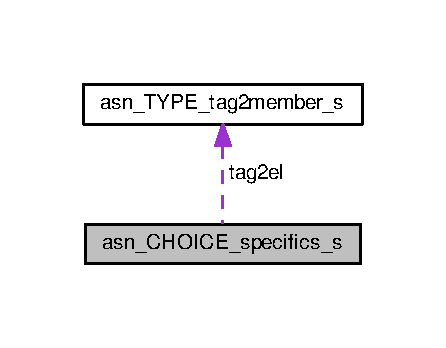
\includegraphics[width=214pt]{structasn__CHOICE__specifics__s__coll__graph}
\end{center}
\end{figure}
\subsection*{Public Attributes}
\begin{DoxyCompactItemize}
\item 
int {\bfseries struct\+\_\+size}\hypertarget{structasn__CHOICE__specifics__s_aa40f554600038ec1f17cc7490b2e573c}{}\label{structasn__CHOICE__specifics__s_aa40f554600038ec1f17cc7490b2e573c}

\item 
int {\bfseries ctx\+\_\+offset}\hypertarget{structasn__CHOICE__specifics__s_aa90321b4f6ced7891aab6185eb195698}{}\label{structasn__CHOICE__specifics__s_aa90321b4f6ced7891aab6185eb195698}

\item 
int {\bfseries pres\+\_\+offset}\hypertarget{structasn__CHOICE__specifics__s_aa179c52e0644ce78896f64e706996fa3}{}\label{structasn__CHOICE__specifics__s_aa179c52e0644ce78896f64e706996fa3}

\item 
int {\bfseries pres\+\_\+size}\hypertarget{structasn__CHOICE__specifics__s_a07835d7982710686c1c0f78666eff09d}{}\label{structasn__CHOICE__specifics__s_a07835d7982710686c1c0f78666eff09d}

\item 
const \hyperlink{structasn__TYPE__tag2member__s}{asn\+\_\+\+T\+Y\+P\+E\+\_\+tag2member\+\_\+t} $\ast$ {\bfseries tag2el}\hypertarget{structasn__CHOICE__specifics__s_ad05a453c35b133f064676d6e2ecabb53}{}\label{structasn__CHOICE__specifics__s_ad05a453c35b133f064676d6e2ecabb53}

\item 
int {\bfseries tag2el\+\_\+count}\hypertarget{structasn__CHOICE__specifics__s_a744b2883930805a8f15b106a3f307ad8}{}\label{structasn__CHOICE__specifics__s_a744b2883930805a8f15b106a3f307ad8}

\item 
int $\ast$ {\bfseries canonical\+\_\+order}\hypertarget{structasn__CHOICE__specifics__s_a9d9568c539045450cd54d61f9e73bf5e}{}\label{structasn__CHOICE__specifics__s_a9d9568c539045450cd54d61f9e73bf5e}

\item 
int {\bfseries ext\+\_\+start}\hypertarget{structasn__CHOICE__specifics__s_a7760292b23a1aa59936300fe8d9e14fe}{}\label{structasn__CHOICE__specifics__s_a7760292b23a1aa59936300fe8d9e14fe}

\end{DoxyCompactItemize}


The documentation for this struct was generated from the following file\+:\begin{DoxyCompactItemize}
\item 
include/aimsun\+\_\+extensions/\+V2\+X\+Framework/\+A\+S\+N1/constr\+\_\+\+C\+H\+O\+I\+C\+E.\+h\end{DoxyCompactItemize}

\hypertarget{structasn__codec__ctx__s}{}\section{asn\+\_\+codec\+\_\+ctx\+\_\+s Struct Reference}
\label{structasn__codec__ctx__s}\index{asn\+\_\+codec\+\_\+ctx\+\_\+s@{asn\+\_\+codec\+\_\+ctx\+\_\+s}}
\subsection*{Public Attributes}
\begin{DoxyCompactItemize}
\item 
size\+\_\+t {\bfseries max\+\_\+stack\+\_\+size}\hypertarget{structasn__codec__ctx__s_a2288d874de0b3366acd79fba3aa20a0c}{}\label{structasn__codec__ctx__s_a2288d874de0b3366acd79fba3aa20a0c}

\end{DoxyCompactItemize}


The documentation for this struct was generated from the following file\+:\begin{DoxyCompactItemize}
\item 
include/aimsun\+\_\+extensions/\+V2\+X\+Framework/\+A\+S\+N1/asn\+\_\+codecs.\+h\end{DoxyCompactItemize}

\hypertarget{structasn__dec__rval__s}{}\section{asn\+\_\+dec\+\_\+rval\+\_\+s Struct Reference}
\label{structasn__dec__rval__s}\index{asn\+\_\+dec\+\_\+rval\+\_\+s@{asn\+\_\+dec\+\_\+rval\+\_\+s}}
\subsection*{Public Attributes}
\begin{DoxyCompactItemize}
\item 
enum asn\+\_\+dec\+\_\+rval\+\_\+code\+\_\+e {\bfseries code}\hypertarget{structasn__dec__rval__s_a5c379ac0e3d6d27d687b6a439123b47f}{}\label{structasn__dec__rval__s_a5c379ac0e3d6d27d687b6a439123b47f}

\item 
size\+\_\+t {\bfseries consumed}\hypertarget{structasn__dec__rval__s_a200882bbdf36418b1a624463b3efad90}{}\label{structasn__dec__rval__s_a200882bbdf36418b1a624463b3efad90}

\end{DoxyCompactItemize}


The documentation for this struct was generated from the following file\+:\begin{DoxyCompactItemize}
\item 
include/aimsun\+\_\+extensions/\+V2\+X\+Framework/\+A\+S\+N1/asn\+\_\+codecs.\+h\end{DoxyCompactItemize}

\hypertarget{structasn__enc__rval__s}{}\section{asn\+\_\+enc\+\_\+rval\+\_\+s Struct Reference}
\label{structasn__enc__rval__s}\index{asn\+\_\+enc\+\_\+rval\+\_\+s@{asn\+\_\+enc\+\_\+rval\+\_\+s}}


Collaboration diagram for asn\+\_\+enc\+\_\+rval\+\_\+s\+:\nopagebreak
\begin{figure}[H]
\begin{center}
\leavevmode
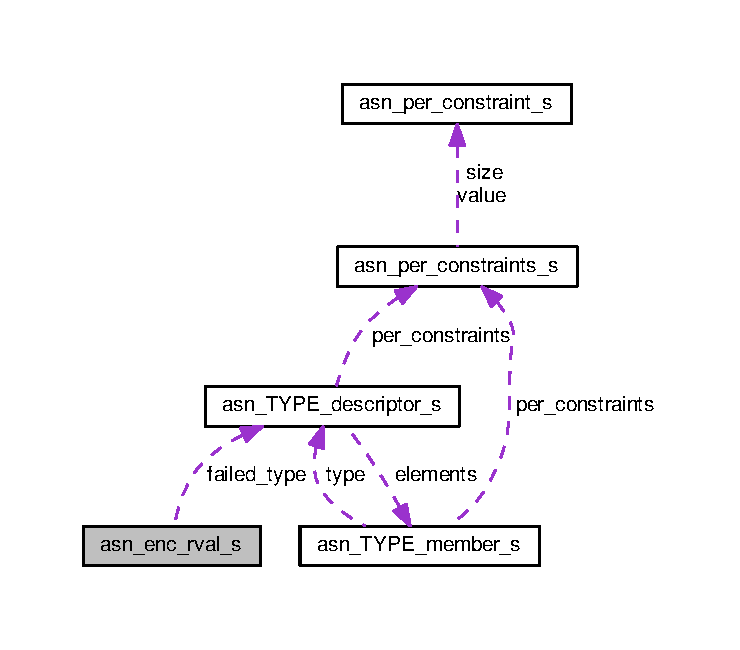
\includegraphics[width=350pt]{structasn__enc__rval__s__coll__graph}
\end{center}
\end{figure}
\subsection*{Public Attributes}
\begin{DoxyCompactItemize}
\item 
ssize\+\_\+t {\bfseries encoded}\hypertarget{structasn__enc__rval__s_ada573b8183a1af819ea3df7a7ea1ba04}{}\label{structasn__enc__rval__s_ada573b8183a1af819ea3df7a7ea1ba04}

\item 
struct \hyperlink{structasn__TYPE__descriptor__s}{asn\+\_\+\+T\+Y\+P\+E\+\_\+descriptor\+\_\+s} $\ast$ {\bfseries failed\+\_\+type}\hypertarget{structasn__enc__rval__s_acee9a75458f1f584db5e913886e9a363}{}\label{structasn__enc__rval__s_acee9a75458f1f584db5e913886e9a363}

\item 
void $\ast$ {\bfseries structure\+\_\+ptr}\hypertarget{structasn__enc__rval__s_a5e01236558d9500760cfa6d679fb6d67}{}\label{structasn__enc__rval__s_a5e01236558d9500760cfa6d679fb6d67}

\end{DoxyCompactItemize}


The documentation for this struct was generated from the following file\+:\begin{DoxyCompactItemize}
\item 
include/aimsun\+\_\+extensions/\+V2\+X\+Framework/\+A\+S\+N1/asn\+\_\+codecs.\+h\end{DoxyCompactItemize}

\hypertarget{structasn__INTEGER__enum__map__s}{}\section{asn\+\_\+\+I\+N\+T\+E\+G\+E\+R\+\_\+enum\+\_\+map\+\_\+s Struct Reference}
\label{structasn__INTEGER__enum__map__s}\index{asn\+\_\+\+I\+N\+T\+E\+G\+E\+R\+\_\+enum\+\_\+map\+\_\+s@{asn\+\_\+\+I\+N\+T\+E\+G\+E\+R\+\_\+enum\+\_\+map\+\_\+s}}
\subsection*{Public Attributes}
\begin{DoxyCompactItemize}
\item 
long {\bfseries nat\+\_\+value}\hypertarget{structasn__INTEGER__enum__map__s_ac14372db4e5264b3136df4fa02e8b18a}{}\label{structasn__INTEGER__enum__map__s_ac14372db4e5264b3136df4fa02e8b18a}

\item 
size\+\_\+t {\bfseries enum\+\_\+len}\hypertarget{structasn__INTEGER__enum__map__s_a55d4c6ad4011cae636878ede3a7de605}{}\label{structasn__INTEGER__enum__map__s_a55d4c6ad4011cae636878ede3a7de605}

\item 
const char $\ast$ {\bfseries enum\+\_\+name}\hypertarget{structasn__INTEGER__enum__map__s_a4f5807a4abd92ba2f1fff3233089f852}{}\label{structasn__INTEGER__enum__map__s_a4f5807a4abd92ba2f1fff3233089f852}

\end{DoxyCompactItemize}


The documentation for this struct was generated from the following file\+:\begin{DoxyCompactItemize}
\item 
include/aimsun\+\_\+extensions/\+V2\+X\+Framework/\+A\+S\+N1/I\+N\+T\+E\+G\+E\+R.\+h\end{DoxyCompactItemize}

\hypertarget{structasn__INTEGER__specifics__s}{}\section{asn\+\_\+\+I\+N\+T\+E\+G\+E\+R\+\_\+specifics\+\_\+s Struct Reference}
\label{structasn__INTEGER__specifics__s}\index{asn\+\_\+\+I\+N\+T\+E\+G\+E\+R\+\_\+specifics\+\_\+s@{asn\+\_\+\+I\+N\+T\+E\+G\+E\+R\+\_\+specifics\+\_\+s}}


Collaboration diagram for asn\+\_\+\+I\+N\+T\+E\+G\+E\+R\+\_\+specifics\+\_\+s\+:\nopagebreak
\begin{figure}[H]
\begin{center}
\leavevmode
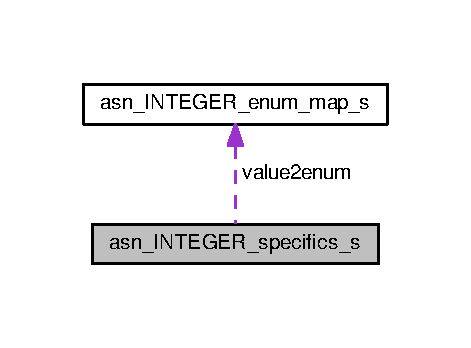
\includegraphics[width=226pt]{structasn__INTEGER__specifics__s__coll__graph}
\end{center}
\end{figure}
\subsection*{Public Attributes}
\begin{DoxyCompactItemize}
\item 
const \hyperlink{structasn__INTEGER__enum__map__s}{asn\+\_\+\+I\+N\+T\+E\+G\+E\+R\+\_\+enum\+\_\+map\+\_\+t} $\ast$ {\bfseries value2enum}\hypertarget{structasn__INTEGER__specifics__s_a5c8b5ba4206844f3ad3b972736634cb6}{}\label{structasn__INTEGER__specifics__s_a5c8b5ba4206844f3ad3b972736634cb6}

\item 
const unsigned int $\ast$ {\bfseries enum2value}\hypertarget{structasn__INTEGER__specifics__s_a643cd7c0a03f05df0070eff704c60776}{}\label{structasn__INTEGER__specifics__s_a643cd7c0a03f05df0070eff704c60776}

\item 
int {\bfseries map\+\_\+count}\hypertarget{structasn__INTEGER__specifics__s_a43f33eddd6e3e6e07226384a4d89ed52}{}\label{structasn__INTEGER__specifics__s_a43f33eddd6e3e6e07226384a4d89ed52}

\item 
int {\bfseries extension}\hypertarget{structasn__INTEGER__specifics__s_a36c822cd98c9bfb311818d36731594aa}{}\label{structasn__INTEGER__specifics__s_a36c822cd98c9bfb311818d36731594aa}

\item 
int {\bfseries strict\+\_\+enumeration}\hypertarget{structasn__INTEGER__specifics__s_a5909a666817ee7a7cab9039bec46012b}{}\label{structasn__INTEGER__specifics__s_a5909a666817ee7a7cab9039bec46012b}

\item 
int {\bfseries field\+\_\+width}\hypertarget{structasn__INTEGER__specifics__s_a91d32a15d5be54f71a67cb6cea80a667}{}\label{structasn__INTEGER__specifics__s_a91d32a15d5be54f71a67cb6cea80a667}

\item 
int {\bfseries field\+\_\+unsigned}\hypertarget{structasn__INTEGER__specifics__s_a86a38acd726911dccc17ce915bafeebc}{}\label{structasn__INTEGER__specifics__s_a86a38acd726911dccc17ce915bafeebc}

\end{DoxyCompactItemize}


The documentation for this struct was generated from the following file\+:\begin{DoxyCompactItemize}
\item 
include/aimsun\+\_\+extensions/\+V2\+X\+Framework/\+A\+S\+N1/I\+N\+T\+E\+G\+E\+R.\+h\end{DoxyCompactItemize}

\hypertarget{structasn__OCTET__STRING__specifics__s}{}\section{asn\+\_\+\+O\+C\+T\+E\+T\+\_\+\+S\+T\+R\+I\+N\+G\+\_\+specifics\+\_\+s Struct Reference}
\label{structasn__OCTET__STRING__specifics__s}\index{asn\+\_\+\+O\+C\+T\+E\+T\+\_\+\+S\+T\+R\+I\+N\+G\+\_\+specifics\+\_\+s@{asn\+\_\+\+O\+C\+T\+E\+T\+\_\+\+S\+T\+R\+I\+N\+G\+\_\+specifics\+\_\+s}}
\subsection*{Public Types}
\begin{DoxyCompactItemize}
\item 
enum {\bfseries asn\+\_\+\+O\+S\+\_\+\+Subvariant} \{ \\*
{\bfseries A\+S\+N\+\_\+\+O\+S\+U\+B\+V\+\_\+\+A\+NY}, 
{\bfseries A\+S\+N\+\_\+\+O\+S\+U\+B\+V\+\_\+\+B\+IT}, 
{\bfseries A\+S\+N\+\_\+\+O\+S\+U\+B\+V\+\_\+\+S\+TR}, 
{\bfseries A\+S\+N\+\_\+\+O\+S\+U\+B\+V\+\_\+\+U16}, 
\\*
{\bfseries A\+S\+N\+\_\+\+O\+S\+U\+B\+V\+\_\+\+U32}
 \}\hypertarget{structasn__OCTET__STRING__specifics__s_a4d3a388a74be4081014f98b6a8a50dd4}{}\label{structasn__OCTET__STRING__specifics__s_a4d3a388a74be4081014f98b6a8a50dd4}

\end{DoxyCompactItemize}
\subsection*{Public Attributes}
\begin{DoxyCompactItemize}
\item 
int {\bfseries struct\+\_\+size}\hypertarget{structasn__OCTET__STRING__specifics__s_a9fe9245c75c076dd503365b33ebddf2d}{}\label{structasn__OCTET__STRING__specifics__s_a9fe9245c75c076dd503365b33ebddf2d}

\item 
int {\bfseries ctx\+\_\+offset}\hypertarget{structasn__OCTET__STRING__specifics__s_a6cf8d330b29cde73baf531c0e42b35ec}{}\label{structasn__OCTET__STRING__specifics__s_a6cf8d330b29cde73baf531c0e42b35ec}

\item 
enum asn\+\_\+\+O\+C\+T\+E\+T\+\_\+\+S\+T\+R\+I\+N\+G\+\_\+specifics\+\_\+s\+::asn\+\_\+\+O\+S\+\_\+\+Subvariant {\bfseries subvariant}\hypertarget{structasn__OCTET__STRING__specifics__s_a7aea52fb2a5970a9adaaaf404cbba224}{}\label{structasn__OCTET__STRING__specifics__s_a7aea52fb2a5970a9adaaaf404cbba224}

\end{DoxyCompactItemize}


The documentation for this struct was generated from the following file\+:\begin{DoxyCompactItemize}
\item 
include/aimsun\+\_\+extensions/\+V2\+X\+Framework/\+A\+S\+N1/O\+C\+T\+E\+T\+\_\+\+S\+T\+R\+I\+N\+G.\+h\end{DoxyCompactItemize}

\hypertarget{structasn__per__constraint__s}{}\section{asn\+\_\+per\+\_\+constraint\+\_\+s Struct Reference}
\label{structasn__per__constraint__s}\index{asn\+\_\+per\+\_\+constraint\+\_\+s@{asn\+\_\+per\+\_\+constraint\+\_\+s}}
\subsection*{Public Types}
\begin{DoxyCompactItemize}
\item 
enum {\bfseries asn\+\_\+per\+\_\+constraint\+\_\+flags} \{ {\bfseries A\+P\+C\+\_\+\+U\+N\+C\+O\+N\+S\+T\+R\+A\+I\+N\+ED} = 0x0, 
{\bfseries A\+P\+C\+\_\+\+S\+E\+M\+I\+\_\+\+C\+O\+N\+S\+T\+R\+A\+I\+N\+ED} = 0x1, 
{\bfseries A\+P\+C\+\_\+\+C\+O\+N\+S\+T\+R\+A\+I\+N\+ED} = 0x2, 
{\bfseries A\+P\+C\+\_\+\+E\+X\+T\+E\+N\+S\+I\+B\+LE} = 0x4
 \}\hypertarget{structasn__per__constraint__s_a7e244d50a6fd6c915949ed844ac1b990}{}\label{structasn__per__constraint__s_a7e244d50a6fd6c915949ed844ac1b990}

\end{DoxyCompactItemize}
\subsection*{Public Attributes}
\begin{DoxyCompactItemize}
\item 
enum asn\+\_\+per\+\_\+constraint\+\_\+s\+::asn\+\_\+per\+\_\+constraint\+\_\+flags {\bfseries flags}\hypertarget{structasn__per__constraint__s_a842536a63e6ea5fe03efe6a6d3453681}{}\label{structasn__per__constraint__s_a842536a63e6ea5fe03efe6a6d3453681}

\item 
int {\bfseries range\+\_\+bits}\hypertarget{structasn__per__constraint__s_aededf9e836382738b542e560d9bb1e50}{}\label{structasn__per__constraint__s_aededf9e836382738b542e560d9bb1e50}

\item 
int {\bfseries effective\+\_\+bits}\hypertarget{structasn__per__constraint__s_a7f6e70444d737a7e4bb8099e07008445}{}\label{structasn__per__constraint__s_a7f6e70444d737a7e4bb8099e07008445}

\item 
long {\bfseries lower\+\_\+bound}\hypertarget{structasn__per__constraint__s_ab3d9a410fde0efb00412226ad51bccea}{}\label{structasn__per__constraint__s_ab3d9a410fde0efb00412226ad51bccea}

\item 
long {\bfseries upper\+\_\+bound}\hypertarget{structasn__per__constraint__s_ac114d50dfb41a04a9448777fc6ad4863}{}\label{structasn__per__constraint__s_ac114d50dfb41a04a9448777fc6ad4863}

\end{DoxyCompactItemize}


The documentation for this struct was generated from the following file\+:\begin{DoxyCompactItemize}
\item 
include/aimsun\+\_\+extensions/\+V2\+X\+Framework/\+A\+S\+N1/per\+\_\+support.\+h\end{DoxyCompactItemize}

\hypertarget{structasn__per__constraints__s}{}\section{asn\+\_\+per\+\_\+constraints\+\_\+s Struct Reference}
\label{structasn__per__constraints__s}\index{asn\+\_\+per\+\_\+constraints\+\_\+s@{asn\+\_\+per\+\_\+constraints\+\_\+s}}


Collaboration diagram for asn\+\_\+per\+\_\+constraints\+\_\+s\+:\nopagebreak
\begin{figure}[H]
\begin{center}
\leavevmode
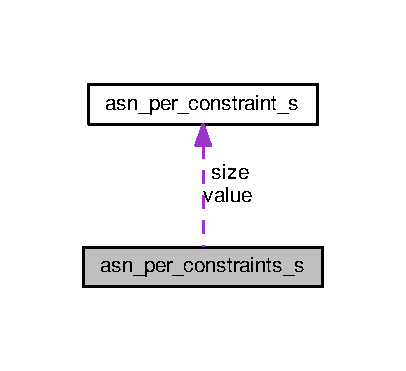
\includegraphics[width=195pt]{structasn__per__constraints__s__coll__graph}
\end{center}
\end{figure}
\subsection*{Public Attributes}
\begin{DoxyCompactItemize}
\item 
struct \hyperlink{structasn__per__constraint__s}{asn\+\_\+per\+\_\+constraint\+\_\+s} {\bfseries value}\hypertarget{structasn__per__constraints__s_a2f4880909e4252c4dc02fda137333ac1}{}\label{structasn__per__constraints__s_a2f4880909e4252c4dc02fda137333ac1}

\item 
struct \hyperlink{structasn__per__constraint__s}{asn\+\_\+per\+\_\+constraint\+\_\+s} {\bfseries size}\hypertarget{structasn__per__constraints__s_aa2c238bac937d10909e541f68a3e773a}{}\label{structasn__per__constraints__s_aa2c238bac937d10909e541f68a3e773a}

\item 
int($\ast$ {\bfseries value2code} )(unsigned int value)\hypertarget{structasn__per__constraints__s_a6cd114154e4dcc184aba1d3537d8d69a}{}\label{structasn__per__constraints__s_a6cd114154e4dcc184aba1d3537d8d69a}

\item 
int($\ast$ {\bfseries code2value} )(unsigned int code)\hypertarget{structasn__per__constraints__s_a7fddc594fa083be79a1ff001879f9cd9}{}\label{structasn__per__constraints__s_a7fddc594fa083be79a1ff001879f9cd9}

\end{DoxyCompactItemize}


The documentation for this struct was generated from the following file\+:\begin{DoxyCompactItemize}
\item 
include/aimsun\+\_\+extensions/\+V2\+X\+Framework/\+A\+S\+N1/per\+\_\+support.\+h\end{DoxyCompactItemize}

\hypertarget{structasn__per__data__s}{}\section{asn\+\_\+per\+\_\+data\+\_\+s Struct Reference}
\label{structasn__per__data__s}\index{asn\+\_\+per\+\_\+data\+\_\+s@{asn\+\_\+per\+\_\+data\+\_\+s}}
\subsection*{Public Attributes}
\begin{DoxyCompactItemize}
\item 
const uint8\+\_\+t $\ast$ {\bfseries buffer}\hypertarget{structasn__per__data__s_a44d99b862f6a541942a64aef1658bbf6}{}\label{structasn__per__data__s_a44d99b862f6a541942a64aef1658bbf6}

\item 
size\+\_\+t {\bfseries nboff}\hypertarget{structasn__per__data__s_a0619c07e943a8b96ae4661f8c5d47582}{}\label{structasn__per__data__s_a0619c07e943a8b96ae4661f8c5d47582}

\item 
size\+\_\+t {\bfseries nbits}\hypertarget{structasn__per__data__s_a11929597749fccb8924b7ae7ecd3935d}{}\label{structasn__per__data__s_a11929597749fccb8924b7ae7ecd3935d}

\item 
size\+\_\+t {\bfseries moved}\hypertarget{structasn__per__data__s_ae457219d0d6f1e0fa24d89af9081ea99}{}\label{structasn__per__data__s_ae457219d0d6f1e0fa24d89af9081ea99}

\item 
int($\ast$ {\bfseries refill} )(struct \hyperlink{structasn__per__data__s}{asn\+\_\+per\+\_\+data\+\_\+s} $\ast$)\hypertarget{structasn__per__data__s_af5327175550501eda70941d045fa3011}{}\label{structasn__per__data__s_af5327175550501eda70941d045fa3011}

\item 
void $\ast$ {\bfseries refill\+\_\+key}\hypertarget{structasn__per__data__s_ab2499e862aa1983fe7df7f65ce088e7e}{}\label{structasn__per__data__s_ab2499e862aa1983fe7df7f65ce088e7e}

\end{DoxyCompactItemize}


The documentation for this struct was generated from the following file\+:\begin{DoxyCompactItemize}
\item 
include/aimsun\+\_\+extensions/\+V2\+X\+Framework/\+A\+S\+N1/per\+\_\+support.\+h\end{DoxyCompactItemize}

\hypertarget{structasn__per__outp__s}{}\section{asn\+\_\+per\+\_\+outp\+\_\+s Struct Reference}
\label{structasn__per__outp__s}\index{asn\+\_\+per\+\_\+outp\+\_\+s@{asn\+\_\+per\+\_\+outp\+\_\+s}}
\subsection*{Public Attributes}
\begin{DoxyCompactItemize}
\item 
uint8\+\_\+t $\ast$ {\bfseries buffer}\hypertarget{structasn__per__outp__s_a48c9ceaafe41b549652f25922c1e0d61}{}\label{structasn__per__outp__s_a48c9ceaafe41b549652f25922c1e0d61}

\item 
size\+\_\+t {\bfseries nboff}\hypertarget{structasn__per__outp__s_a414cbcccffad5a86b0d51166cc1eb94d}{}\label{structasn__per__outp__s_a414cbcccffad5a86b0d51166cc1eb94d}

\item 
size\+\_\+t {\bfseries nbits}\hypertarget{structasn__per__outp__s_a0d23210c600b088d271ee475c83da9ba}{}\label{structasn__per__outp__s_a0d23210c600b088d271ee475c83da9ba}

\item 
uint8\+\_\+t {\bfseries tmpspace} \mbox{[}32\mbox{]}\hypertarget{structasn__per__outp__s_ac13d0f08ae74c6f48d6706bb21d61c18}{}\label{structasn__per__outp__s_ac13d0f08ae74c6f48d6706bb21d61c18}

\item 
int($\ast$ {\bfseries outper} )(const void $\ast$data, size\+\_\+t size, void $\ast$op\+\_\+key)\hypertarget{structasn__per__outp__s_afaa9fd277b0ca190698086b4d42395ea}{}\label{structasn__per__outp__s_afaa9fd277b0ca190698086b4d42395ea}

\item 
void $\ast$ {\bfseries op\+\_\+key}\hypertarget{structasn__per__outp__s_ae5804721478d885d76994fafd9d8c67e}{}\label{structasn__per__outp__s_ae5804721478d885d76994fafd9d8c67e}

\item 
size\+\_\+t {\bfseries flushed\+\_\+bytes}\hypertarget{structasn__per__outp__s_a972e9580e422c7f2bfc576d129adc1ac}{}\label{structasn__per__outp__s_a972e9580e422c7f2bfc576d129adc1ac}

\end{DoxyCompactItemize}


The documentation for this struct was generated from the following file\+:\begin{DoxyCompactItemize}
\item 
include/aimsun\+\_\+extensions/\+V2\+X\+Framework/\+A\+S\+N1/per\+\_\+support.\+h\end{DoxyCompactItemize}

\hypertarget{structasn__SEQUENCE__specifics__s}{}\section{asn\+\_\+\+S\+E\+Q\+U\+E\+N\+C\+E\+\_\+specifics\+\_\+s Struct Reference}
\label{structasn__SEQUENCE__specifics__s}\index{asn\+\_\+\+S\+E\+Q\+U\+E\+N\+C\+E\+\_\+specifics\+\_\+s@{asn\+\_\+\+S\+E\+Q\+U\+E\+N\+C\+E\+\_\+specifics\+\_\+s}}


Collaboration diagram for asn\+\_\+\+S\+E\+Q\+U\+E\+N\+C\+E\+\_\+specifics\+\_\+s\+:\nopagebreak
\begin{figure}[H]
\begin{center}
\leavevmode
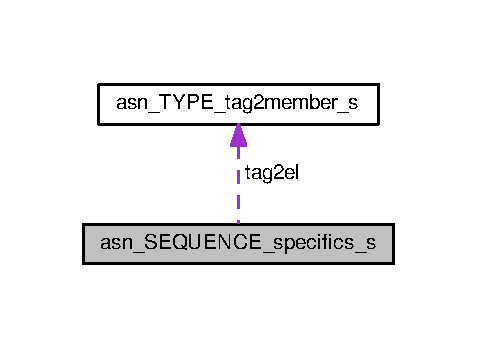
\includegraphics[width=229pt]{structasn__SEQUENCE__specifics__s__coll__graph}
\end{center}
\end{figure}
\subsection*{Public Attributes}
\begin{DoxyCompactItemize}
\item 
int {\bfseries struct\+\_\+size}\hypertarget{structasn__SEQUENCE__specifics__s_a45bfbd26bc54a36d8bb94a27dfdddeab}{}\label{structasn__SEQUENCE__specifics__s_a45bfbd26bc54a36d8bb94a27dfdddeab}

\item 
int {\bfseries ctx\+\_\+offset}\hypertarget{structasn__SEQUENCE__specifics__s_ae6fc81ca5dbc4f5a91d60fe0366119c7}{}\label{structasn__SEQUENCE__specifics__s_ae6fc81ca5dbc4f5a91d60fe0366119c7}

\item 
const \hyperlink{structasn__TYPE__tag2member__s}{asn\+\_\+\+T\+Y\+P\+E\+\_\+tag2member\+\_\+t} $\ast$ {\bfseries tag2el}\hypertarget{structasn__SEQUENCE__specifics__s_a3798278dcde75da87060a567f4bbbb05}{}\label{structasn__SEQUENCE__specifics__s_a3798278dcde75da87060a567f4bbbb05}

\item 
int {\bfseries tag2el\+\_\+count}\hypertarget{structasn__SEQUENCE__specifics__s_a8bd72748029938524a1bea5c8c73b88a}{}\label{structasn__SEQUENCE__specifics__s_a8bd72748029938524a1bea5c8c73b88a}

\item 
const int $\ast$ {\bfseries oms}\hypertarget{structasn__SEQUENCE__specifics__s_a0bbe76bec7ecff31a3234b7fa3414e38}{}\label{structasn__SEQUENCE__specifics__s_a0bbe76bec7ecff31a3234b7fa3414e38}

\item 
int {\bfseries roms\+\_\+count}\hypertarget{structasn__SEQUENCE__specifics__s_a0ec9ecedf8ff6b25a8a4e8b51a0e7b7e}{}\label{structasn__SEQUENCE__specifics__s_a0ec9ecedf8ff6b25a8a4e8b51a0e7b7e}

\item 
int {\bfseries aoms\+\_\+count}\hypertarget{structasn__SEQUENCE__specifics__s_ab3f160f58d19eea92aca727cb5e3fce2}{}\label{structasn__SEQUENCE__specifics__s_ab3f160f58d19eea92aca727cb5e3fce2}

\item 
int {\bfseries ext\+\_\+after}\hypertarget{structasn__SEQUENCE__specifics__s_aa77ae8ec487140bc0b3f82eba3041160}{}\label{structasn__SEQUENCE__specifics__s_aa77ae8ec487140bc0b3f82eba3041160}

\item 
int {\bfseries ext\+\_\+before}\hypertarget{structasn__SEQUENCE__specifics__s_a844b9a047a3b9206713725fb9fdde94b}{}\label{structasn__SEQUENCE__specifics__s_a844b9a047a3b9206713725fb9fdde94b}

\end{DoxyCompactItemize}


The documentation for this struct was generated from the following file\+:\begin{DoxyCompactItemize}
\item 
include/aimsun\+\_\+extensions/\+V2\+X\+Framework/\+A\+S\+N1/constr\+\_\+\+S\+E\+Q\+U\+E\+N\+C\+E.\+h\end{DoxyCompactItemize}

\hypertarget{structasn__SET__OF__specifics__s}{}\section{asn\+\_\+\+S\+E\+T\+\_\+\+O\+F\+\_\+specifics\+\_\+s Struct Reference}
\label{structasn__SET__OF__specifics__s}\index{asn\+\_\+\+S\+E\+T\+\_\+\+O\+F\+\_\+specifics\+\_\+s@{asn\+\_\+\+S\+E\+T\+\_\+\+O\+F\+\_\+specifics\+\_\+s}}
\subsection*{Public Attributes}
\begin{DoxyCompactItemize}
\item 
int {\bfseries struct\+\_\+size}\hypertarget{structasn__SET__OF__specifics__s_a441cca370f35fd73e231ffa1923d0dc2}{}\label{structasn__SET__OF__specifics__s_a441cca370f35fd73e231ffa1923d0dc2}

\item 
int {\bfseries ctx\+\_\+offset}\hypertarget{structasn__SET__OF__specifics__s_a1af400a4257bf2dd278ed11c254a4df4}{}\label{structasn__SET__OF__specifics__s_a1af400a4257bf2dd278ed11c254a4df4}

\item 
int {\bfseries as\+\_\+\+X\+M\+L\+Value\+List}\hypertarget{structasn__SET__OF__specifics__s_a01f688079a44819a7647c4b5900fd2c6}{}\label{structasn__SET__OF__specifics__s_a01f688079a44819a7647c4b5900fd2c6}

\end{DoxyCompactItemize}


The documentation for this struct was generated from the following file\+:\begin{DoxyCompactItemize}
\item 
include/aimsun\+\_\+extensions/\+V2\+X\+Framework/\+A\+S\+N1/constr\+\_\+\+S\+E\+T\+\_\+\+O\+F.\+h\end{DoxyCompactItemize}

\hypertarget{structasn__SET__specifics__s}{}\section{asn\+\_\+\+S\+E\+T\+\_\+specifics\+\_\+s Struct Reference}
\label{structasn__SET__specifics__s}\index{asn\+\_\+\+S\+E\+T\+\_\+specifics\+\_\+s@{asn\+\_\+\+S\+E\+T\+\_\+specifics\+\_\+s}}


Collaboration diagram for asn\+\_\+\+S\+E\+T\+\_\+specifics\+\_\+s\+:\nopagebreak
\begin{figure}[H]
\begin{center}
\leavevmode
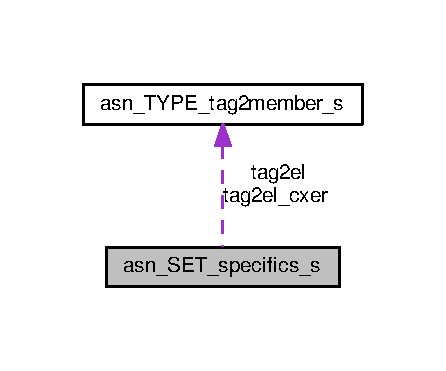
\includegraphics[width=214pt]{structasn__SET__specifics__s__coll__graph}
\end{center}
\end{figure}
\subsection*{Public Attributes}
\begin{DoxyCompactItemize}
\item 
int {\bfseries struct\+\_\+size}\hypertarget{structasn__SET__specifics__s_a7980cedae581d9a54df6e5f4cd3ace69}{}\label{structasn__SET__specifics__s_a7980cedae581d9a54df6e5f4cd3ace69}

\item 
int {\bfseries ctx\+\_\+offset}\hypertarget{structasn__SET__specifics__s_a11686de14a23286844e426092af44cdc}{}\label{structasn__SET__specifics__s_a11686de14a23286844e426092af44cdc}

\item 
int {\bfseries pres\+\_\+offset}\hypertarget{structasn__SET__specifics__s_a53ddd3d0b0fdf99a139807e7580c2247}{}\label{structasn__SET__specifics__s_a53ddd3d0b0fdf99a139807e7580c2247}

\item 
const \hyperlink{structasn__TYPE__tag2member__s}{asn\+\_\+\+T\+Y\+P\+E\+\_\+tag2member\+\_\+t} $\ast$ {\bfseries tag2el}\hypertarget{structasn__SET__specifics__s_a5cfec9d469715aa3585d135720fc0e0c}{}\label{structasn__SET__specifics__s_a5cfec9d469715aa3585d135720fc0e0c}

\item 
int {\bfseries tag2el\+\_\+count}\hypertarget{structasn__SET__specifics__s_a39f9806086eb4a6d2c1126e55eb05b81}{}\label{structasn__SET__specifics__s_a39f9806086eb4a6d2c1126e55eb05b81}

\item 
const \hyperlink{structasn__TYPE__tag2member__s}{asn\+\_\+\+T\+Y\+P\+E\+\_\+tag2member\+\_\+t} $\ast$ {\bfseries tag2el\+\_\+cxer}\hypertarget{structasn__SET__specifics__s_a01e19ad8b6ea2c0d53096744372aef9e}{}\label{structasn__SET__specifics__s_a01e19ad8b6ea2c0d53096744372aef9e}

\item 
int {\bfseries tag2el\+\_\+cxer\+\_\+count}\hypertarget{structasn__SET__specifics__s_a294e7fcfb45153ce8b776db4547303bc}{}\label{structasn__SET__specifics__s_a294e7fcfb45153ce8b776db4547303bc}

\item 
int {\bfseries extensible}\hypertarget{structasn__SET__specifics__s_aaf4f5d75a884a5a6c1dc24690a533191}{}\label{structasn__SET__specifics__s_aaf4f5d75a884a5a6c1dc24690a533191}

\item 
const unsigned int $\ast$ {\bfseries \+\_\+mandatory\+\_\+elements}\hypertarget{structasn__SET__specifics__s_a86fb45d623bde89a343eb2bda86bbf5e}{}\label{structasn__SET__specifics__s_a86fb45d623bde89a343eb2bda86bbf5e}

\end{DoxyCompactItemize}


The documentation for this struct was generated from the following file\+:\begin{DoxyCompactItemize}
\item 
include/aimsun\+\_\+extensions/\+V2\+X\+Framework/\+A\+S\+N1/constr\+\_\+\+S\+E\+T.\+h\end{DoxyCompactItemize}

\hypertarget{structasn__struct__ctx__s}{}\section{asn\+\_\+struct\+\_\+ctx\+\_\+s Struct Reference}
\label{structasn__struct__ctx__s}\index{asn\+\_\+struct\+\_\+ctx\+\_\+s@{asn\+\_\+struct\+\_\+ctx\+\_\+s}}
\subsection*{Public Attributes}
\begin{DoxyCompactItemize}
\item 
short {\bfseries phase}\hypertarget{structasn__struct__ctx__s_a34c3cbadc60f33eddb20095ab397a9c4}{}\label{structasn__struct__ctx__s_a34c3cbadc60f33eddb20095ab397a9c4}

\item 
short {\bfseries step}\hypertarget{structasn__struct__ctx__s_ac1bd97e26ed31920941bcb44edca5514}{}\label{structasn__struct__ctx__s_ac1bd97e26ed31920941bcb44edca5514}

\item 
int {\bfseries context}\hypertarget{structasn__struct__ctx__s_a969440b1f76b63cc5f739df9ec127f5c}{}\label{structasn__struct__ctx__s_a969440b1f76b63cc5f739df9ec127f5c}

\item 
void $\ast$ {\bfseries ptr}\hypertarget{structasn__struct__ctx__s_a85a8df91ee53fb5c2d9232a62d792f93}{}\label{structasn__struct__ctx__s_a85a8df91ee53fb5c2d9232a62d792f93}

\item 
ber\+\_\+tlv\+\_\+len\+\_\+t {\bfseries left}\hypertarget{structasn__struct__ctx__s_adfba2796328af7c6054fadaf22b4ed6b}{}\label{structasn__struct__ctx__s_adfba2796328af7c6054fadaf22b4ed6b}

\end{DoxyCompactItemize}


The documentation for this struct was generated from the following file\+:\begin{DoxyCompactItemize}
\item 
include/aimsun\+\_\+extensions/\+V2\+X\+Framework/\+A\+S\+N1/constr\+\_\+\+T\+Y\+P\+E.\+h\end{DoxyCompactItemize}

\hypertarget{structasn__TYPE__descriptor__s}{}\section{asn\+\_\+\+T\+Y\+P\+E\+\_\+descriptor\+\_\+s Struct Reference}
\label{structasn__TYPE__descriptor__s}\index{asn\+\_\+\+T\+Y\+P\+E\+\_\+descriptor\+\_\+s@{asn\+\_\+\+T\+Y\+P\+E\+\_\+descriptor\+\_\+s}}


Collaboration diagram for asn\+\_\+\+T\+Y\+P\+E\+\_\+descriptor\+\_\+s\+:\nopagebreak
\begin{figure}[H]
\begin{center}
\leavevmode
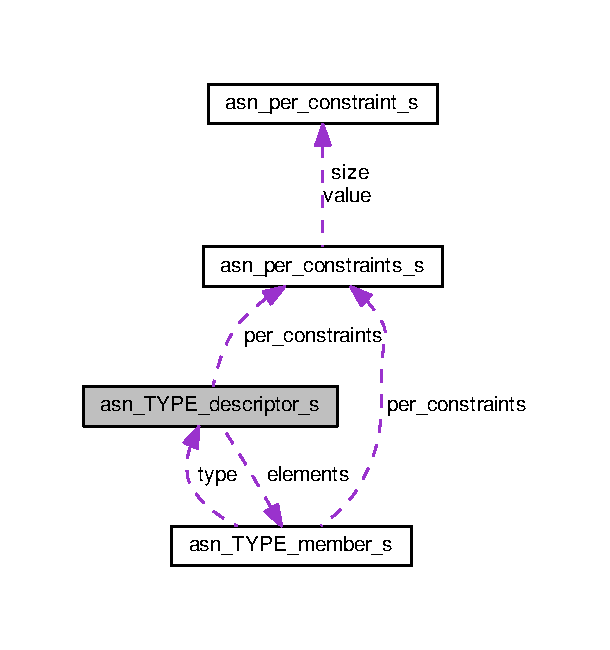
\includegraphics[width=293pt]{structasn__TYPE__descriptor__s__coll__graph}
\end{center}
\end{figure}
\subsection*{Public Attributes}
\begin{DoxyCompactItemize}
\item 
const char $\ast$ {\bfseries name}\hypertarget{structasn__TYPE__descriptor__s_a8a8966744e76300bbcf4b18acfba6583}{}\label{structasn__TYPE__descriptor__s_a8a8966744e76300bbcf4b18acfba6583}

\item 
const char $\ast$ {\bfseries xml\+\_\+tag}\hypertarget{structasn__TYPE__descriptor__s_a5a54d0f35790598d15c38e20e26d0c62}{}\label{structasn__TYPE__descriptor__s_a5a54d0f35790598d15c38e20e26d0c62}

\item 
asn\+\_\+struct\+\_\+free\+\_\+f $\ast$ {\bfseries free\+\_\+struct}\hypertarget{structasn__TYPE__descriptor__s_a9582a3b6bf69f704147a84293996bc87}{}\label{structasn__TYPE__descriptor__s_a9582a3b6bf69f704147a84293996bc87}

\item 
asn\+\_\+struct\+\_\+print\+\_\+f $\ast$ {\bfseries print\+\_\+struct}\hypertarget{structasn__TYPE__descriptor__s_ae95ed405f6b0d12dd83a2f7415b23563}{}\label{structasn__TYPE__descriptor__s_ae95ed405f6b0d12dd83a2f7415b23563}

\item 
asn\+\_\+constr\+\_\+check\+\_\+f $\ast$ {\bfseries check\+\_\+constraints}\hypertarget{structasn__TYPE__descriptor__s_aa0cc7d278b7ecef7f83c25da3c73c0d9}{}\label{structasn__TYPE__descriptor__s_aa0cc7d278b7ecef7f83c25da3c73c0d9}

\item 
ber\+\_\+type\+\_\+decoder\+\_\+f $\ast$ {\bfseries ber\+\_\+decoder}\hypertarget{structasn__TYPE__descriptor__s_ab4d569207532fe71a3f2cb0f25d0a25f}{}\label{structasn__TYPE__descriptor__s_ab4d569207532fe71a3f2cb0f25d0a25f}

\item 
der\+\_\+type\+\_\+encoder\+\_\+f $\ast$ {\bfseries der\+\_\+encoder}\hypertarget{structasn__TYPE__descriptor__s_a8babc45f0567d8de5f2e403acdb9d9ad}{}\label{structasn__TYPE__descriptor__s_a8babc45f0567d8de5f2e403acdb9d9ad}

\item 
xer\+\_\+type\+\_\+decoder\+\_\+f $\ast$ {\bfseries xer\+\_\+decoder}\hypertarget{structasn__TYPE__descriptor__s_a1234d8ff33b0b6b3a47439546bf3db78}{}\label{structasn__TYPE__descriptor__s_a1234d8ff33b0b6b3a47439546bf3db78}

\item 
xer\+\_\+type\+\_\+encoder\+\_\+f $\ast$ {\bfseries xer\+\_\+encoder}\hypertarget{structasn__TYPE__descriptor__s_a003bac9c6861ee39ec184a6b3c33eae9}{}\label{structasn__TYPE__descriptor__s_a003bac9c6861ee39ec184a6b3c33eae9}

\item 
per\+\_\+type\+\_\+decoder\+\_\+f $\ast$ {\bfseries uper\+\_\+decoder}\hypertarget{structasn__TYPE__descriptor__s_a1ddbe64c1964522f5099f65b12597314}{}\label{structasn__TYPE__descriptor__s_a1ddbe64c1964522f5099f65b12597314}

\item 
per\+\_\+type\+\_\+encoder\+\_\+f $\ast$ {\bfseries uper\+\_\+encoder}\hypertarget{structasn__TYPE__descriptor__s_af281bfde376967284027748b9bcee2a0}{}\label{structasn__TYPE__descriptor__s_af281bfde376967284027748b9bcee2a0}

\item 
asn\+\_\+outmost\+\_\+tag\+\_\+f $\ast$ {\bfseries outmost\+\_\+tag}\hypertarget{structasn__TYPE__descriptor__s_a52d908ab49412902c959f79735b95354}{}\label{structasn__TYPE__descriptor__s_a52d908ab49412902c959f79735b95354}

\item 
const ber\+\_\+tlv\+\_\+tag\+\_\+t $\ast$ {\bfseries tags}\hypertarget{structasn__TYPE__descriptor__s_a7e85f1690f7ae701bae048c01ba102ab}{}\label{structasn__TYPE__descriptor__s_a7e85f1690f7ae701bae048c01ba102ab}

\item 
int {\bfseries tags\+\_\+count}\hypertarget{structasn__TYPE__descriptor__s_a5d2ce485a26f3af96fdd706f4ac37c11}{}\label{structasn__TYPE__descriptor__s_a5d2ce485a26f3af96fdd706f4ac37c11}

\item 
const ber\+\_\+tlv\+\_\+tag\+\_\+t $\ast$ {\bfseries all\+\_\+tags}\hypertarget{structasn__TYPE__descriptor__s_ae2bab4db1f3a80a74b26f096b347ad49}{}\label{structasn__TYPE__descriptor__s_ae2bab4db1f3a80a74b26f096b347ad49}

\item 
int {\bfseries all\+\_\+tags\+\_\+count}\hypertarget{structasn__TYPE__descriptor__s_a30b662834a29871aad815dc8ff886bb2}{}\label{structasn__TYPE__descriptor__s_a30b662834a29871aad815dc8ff886bb2}

\item 
\hyperlink{structasn__per__constraints__s}{asn\+\_\+per\+\_\+constraints\+\_\+t} $\ast$ {\bfseries per\+\_\+constraints}\hypertarget{structasn__TYPE__descriptor__s_aeb1a012320b4907334d1cf5ece41085b}{}\label{structasn__TYPE__descriptor__s_aeb1a012320b4907334d1cf5ece41085b}

\item 
struct \hyperlink{structasn__TYPE__member__s}{asn\+\_\+\+T\+Y\+P\+E\+\_\+member\+\_\+s} $\ast$ {\bfseries elements}\hypertarget{structasn__TYPE__descriptor__s_ad4b966ba4a3e7511b59933cf1d0b8200}{}\label{structasn__TYPE__descriptor__s_ad4b966ba4a3e7511b59933cf1d0b8200}

\item 
int {\bfseries elements\+\_\+count}\hypertarget{structasn__TYPE__descriptor__s_ac26bd7451f4f8b84cf30952c74e2ef0b}{}\label{structasn__TYPE__descriptor__s_ac26bd7451f4f8b84cf30952c74e2ef0b}

\item 
const void $\ast$ {\bfseries specifics}\hypertarget{structasn__TYPE__descriptor__s_a872c82d21e1ee31ba377d9ba31c6095d}{}\label{structasn__TYPE__descriptor__s_a872c82d21e1ee31ba377d9ba31c6095d}

\end{DoxyCompactItemize}


The documentation for this struct was generated from the following file\+:\begin{DoxyCompactItemize}
\item 
include/aimsun\+\_\+extensions/\+V2\+X\+Framework/\+A\+S\+N1/constr\+\_\+\+T\+Y\+P\+E.\+h\end{DoxyCompactItemize}

\hypertarget{structasn__TYPE__member__s}{}\section{asn\+\_\+\+T\+Y\+P\+E\+\_\+member\+\_\+s Struct Reference}
\label{structasn__TYPE__member__s}\index{asn\+\_\+\+T\+Y\+P\+E\+\_\+member\+\_\+s@{asn\+\_\+\+T\+Y\+P\+E\+\_\+member\+\_\+s}}


Collaboration diagram for asn\+\_\+\+T\+Y\+P\+E\+\_\+member\+\_\+s\+:\nopagebreak
\begin{figure}[H]
\begin{center}
\leavevmode
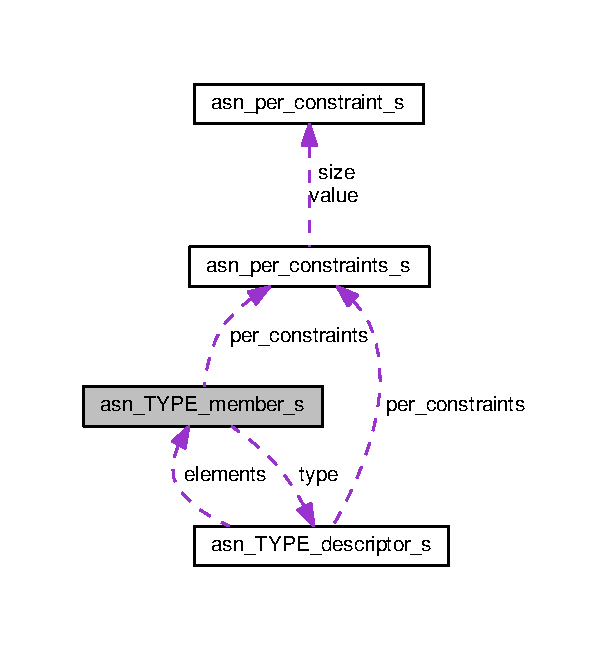
\includegraphics[width=293pt]{structasn__TYPE__member__s__coll__graph}
\end{center}
\end{figure}
\subsection*{Public Attributes}
\begin{DoxyCompactItemize}
\item 
enum asn\+\_\+\+T\+Y\+P\+E\+\_\+flags\+\_\+e {\bfseries flags}\hypertarget{structasn__TYPE__member__s_ad68a2e56242af0712af99fa75cff3406}{}\label{structasn__TYPE__member__s_ad68a2e56242af0712af99fa75cff3406}

\item 
int {\bfseries optional}\hypertarget{structasn__TYPE__member__s_aefa11aa34e9e47b0ebcdcbe5b66dc96f}{}\label{structasn__TYPE__member__s_aefa11aa34e9e47b0ebcdcbe5b66dc96f}

\item 
int {\bfseries memb\+\_\+offset}\hypertarget{structasn__TYPE__member__s_a80a62dea12ff1b6e587fd0af97c4823c}{}\label{structasn__TYPE__member__s_a80a62dea12ff1b6e587fd0af97c4823c}

\item 
ber\+\_\+tlv\+\_\+tag\+\_\+t {\bfseries tag}\hypertarget{structasn__TYPE__member__s_a7b1bd68f8a254c0e87c31985d71d500e}{}\label{structasn__TYPE__member__s_a7b1bd68f8a254c0e87c31985d71d500e}

\item 
int {\bfseries tag\+\_\+mode}\hypertarget{structasn__TYPE__member__s_a0e066b601beba109db9ed2c98b4ec63c}{}\label{structasn__TYPE__member__s_a0e066b601beba109db9ed2c98b4ec63c}

\item 
\hyperlink{structasn__TYPE__descriptor__s}{asn\+\_\+\+T\+Y\+P\+E\+\_\+descriptor\+\_\+t} $\ast$ {\bfseries type}\hypertarget{structasn__TYPE__member__s_a03213b5d84dc8a92c49685f24aaf83ea}{}\label{structasn__TYPE__member__s_a03213b5d84dc8a92c49685f24aaf83ea}

\item 
asn\+\_\+constr\+\_\+check\+\_\+f $\ast$ {\bfseries memb\+\_\+constraints}\hypertarget{structasn__TYPE__member__s_af9e152adaff281b054caf70ba1865e82}{}\label{structasn__TYPE__member__s_af9e152adaff281b054caf70ba1865e82}

\item 
\hyperlink{structasn__per__constraints__s}{asn\+\_\+per\+\_\+constraints\+\_\+t} $\ast$ {\bfseries per\+\_\+constraints}\hypertarget{structasn__TYPE__member__s_ad92283728040413ca70956874344436a}{}\label{structasn__TYPE__member__s_ad92283728040413ca70956874344436a}

\item 
int($\ast$ {\bfseries default\+\_\+value} )(int setval, void $\ast$$\ast$sptr)\hypertarget{structasn__TYPE__member__s_ab68957350003d9a2f11e548a3ef1088f}{}\label{structasn__TYPE__member__s_ab68957350003d9a2f11e548a3ef1088f}

\item 
const char $\ast$ {\bfseries name}\hypertarget{structasn__TYPE__member__s_a9b03b2a79aa01871dae00c6579e2be17}{}\label{structasn__TYPE__member__s_a9b03b2a79aa01871dae00c6579e2be17}

\end{DoxyCompactItemize}


The documentation for this struct was generated from the following file\+:\begin{DoxyCompactItemize}
\item 
include/aimsun\+\_\+extensions/\+V2\+X\+Framework/\+A\+S\+N1/constr\+\_\+\+T\+Y\+P\+E.\+h\end{DoxyCompactItemize}

\hypertarget{structasn__TYPE__tag2member__s}{}\section{asn\+\_\+\+T\+Y\+P\+E\+\_\+tag2member\+\_\+s Struct Reference}
\label{structasn__TYPE__tag2member__s}\index{asn\+\_\+\+T\+Y\+P\+E\+\_\+tag2member\+\_\+s@{asn\+\_\+\+T\+Y\+P\+E\+\_\+tag2member\+\_\+s}}
\subsection*{Public Attributes}
\begin{DoxyCompactItemize}
\item 
ber\+\_\+tlv\+\_\+tag\+\_\+t {\bfseries el\+\_\+tag}\hypertarget{structasn__TYPE__tag2member__s_a5e6c60c9b693dfe75f474b874ceb5553}{}\label{structasn__TYPE__tag2member__s_a5e6c60c9b693dfe75f474b874ceb5553}

\item 
int {\bfseries el\+\_\+no}\hypertarget{structasn__TYPE__tag2member__s_aa4cc00d29362751105f5440956084cf6}{}\label{structasn__TYPE__tag2member__s_aa4cc00d29362751105f5440956084cf6}

\item 
int {\bfseries toff\+\_\+first}\hypertarget{structasn__TYPE__tag2member__s_aa142c0183296929729d180377f418a56}{}\label{structasn__TYPE__tag2member__s_aa142c0183296929729d180377f418a56}

\item 
int {\bfseries toff\+\_\+last}\hypertarget{structasn__TYPE__tag2member__s_a5ecd9b207d1e711e3791bdb33080b862}{}\label{structasn__TYPE__tag2member__s_a5ecd9b207d1e711e3791bdb33080b862}

\end{DoxyCompactItemize}


The documentation for this struct was generated from the following file\+:\begin{DoxyCompactItemize}
\item 
include/aimsun\+\_\+extensions/\+V2\+X\+Framework/\+A\+S\+N1/constr\+\_\+\+T\+Y\+P\+E.\+h\end{DoxyCompactItemize}

\hypertarget{structAttributeIdList}{}\section{Attribute\+Id\+List Struct Reference}
\label{structAttributeIdList}\index{Attribute\+Id\+List@{Attribute\+Id\+List}}


Collaboration diagram for Attribute\+Id\+List\+:\nopagebreak
\begin{figure}[H]
\begin{center}
\leavevmode
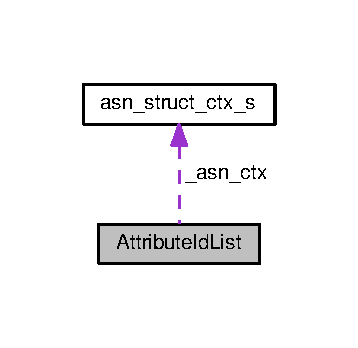
\includegraphics[width=172pt]{structAttributeIdList__coll__graph}
\end{center}
\end{figure}
\subsection*{Public Member Functions}
\begin{DoxyCompactItemize}
\item 
{\bfseries A\+\_\+\+S\+E\+Q\+U\+E\+N\+C\+E\+\_\+\+OF} (long) list\hypertarget{structAttributeIdList_a8aa113a4f3993b47a1ab56addc19cb01}{}\label{structAttributeIdList_a8aa113a4f3993b47a1ab56addc19cb01}

\end{DoxyCompactItemize}
\subsection*{Public Attributes}
\begin{DoxyCompactItemize}
\item 
\hyperlink{structasn__struct__ctx__s}{asn\+\_\+struct\+\_\+ctx\+\_\+t} {\bfseries \+\_\+asn\+\_\+ctx}\hypertarget{structAttributeIdList_af9f5beaad5241513105d367acf31537a}{}\label{structAttributeIdList_af9f5beaad5241513105d367acf31537a}

\end{DoxyCompactItemize}


The documentation for this struct was generated from the following file\+:\begin{DoxyCompactItemize}
\item 
include/aimsun\+\_\+extensions/\+V2\+X\+Framework/\+I\+T\+S-\/spec/Attribute\+Id\+List.\+h\end{DoxyCompactItemize}

\hypertarget{structAxleWeightLimits}{}\section{Axle\+Weight\+Limits Struct Reference}
\label{structAxleWeightLimits}\index{Axle\+Weight\+Limits@{Axle\+Weight\+Limits}}


Collaboration diagram for Axle\+Weight\+Limits\+:\nopagebreak
\begin{figure}[H]
\begin{center}
\leavevmode
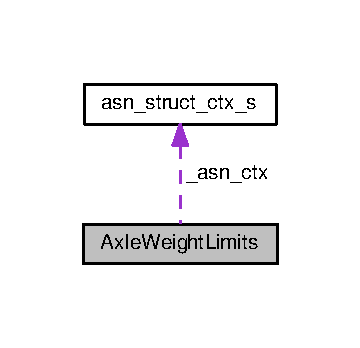
\includegraphics[width=173pt]{structAxleWeightLimits__coll__graph}
\end{center}
\end{figure}
\subsection*{Public Attributes}
\begin{DoxyCompactItemize}
\item 
Int2\+\_\+t {\bfseries max\+Ladenweight\+On\+Axle1}\hypertarget{structAxleWeightLimits_ae786bb78361773b06e7b09fa77090d06}{}\label{structAxleWeightLimits_ae786bb78361773b06e7b09fa77090d06}

\item 
Int2\+\_\+t {\bfseries max\+Ladenweight\+On\+Axle2}\hypertarget{structAxleWeightLimits_a0f76443b641175173acb823c71e8a56e}{}\label{structAxleWeightLimits_a0f76443b641175173acb823c71e8a56e}

\item 
Int2\+\_\+t {\bfseries max\+Ladenweight\+On\+Axle3}\hypertarget{structAxleWeightLimits_ab889c72a9015f6f184644fe4616176a0}{}\label{structAxleWeightLimits_ab889c72a9015f6f184644fe4616176a0}

\item 
Int2\+\_\+t {\bfseries max\+Ladenweight\+On\+Axle4}\hypertarget{structAxleWeightLimits_a558e61dcae006b24b9a0a575ce5a5779}{}\label{structAxleWeightLimits_a558e61dcae006b24b9a0a575ce5a5779}

\item 
Int2\+\_\+t {\bfseries max\+Ladenweight\+On\+Axle5}\hypertarget{structAxleWeightLimits_a84e049c5ebe1d7d9f942d3eeb4e319e3}{}\label{structAxleWeightLimits_a84e049c5ebe1d7d9f942d3eeb4e319e3}

\item 
\hyperlink{structasn__struct__ctx__s}{asn\+\_\+struct\+\_\+ctx\+\_\+t} {\bfseries \+\_\+asn\+\_\+ctx}\hypertarget{structAxleWeightLimits_af23bd9bea4371695528ec37a7eebc28e}{}\label{structAxleWeightLimits_af23bd9bea4371695528ec37a7eebc28e}

\end{DoxyCompactItemize}


The documentation for this struct was generated from the following file\+:\begin{DoxyCompactItemize}
\item 
include/aimsun\+\_\+extensions/\+V2\+X\+Framework/\+I\+T\+S-\/spec/Axle\+Weight\+Limits.\+h\end{DoxyCompactItemize}

\hypertarget{structBasicContainer}{}\section{Basic\+Container Struct Reference}
\label{structBasicContainer}\index{Basic\+Container@{Basic\+Container}}


Collaboration diagram for Basic\+Container\+:\nopagebreak
\begin{figure}[H]
\begin{center}
\leavevmode
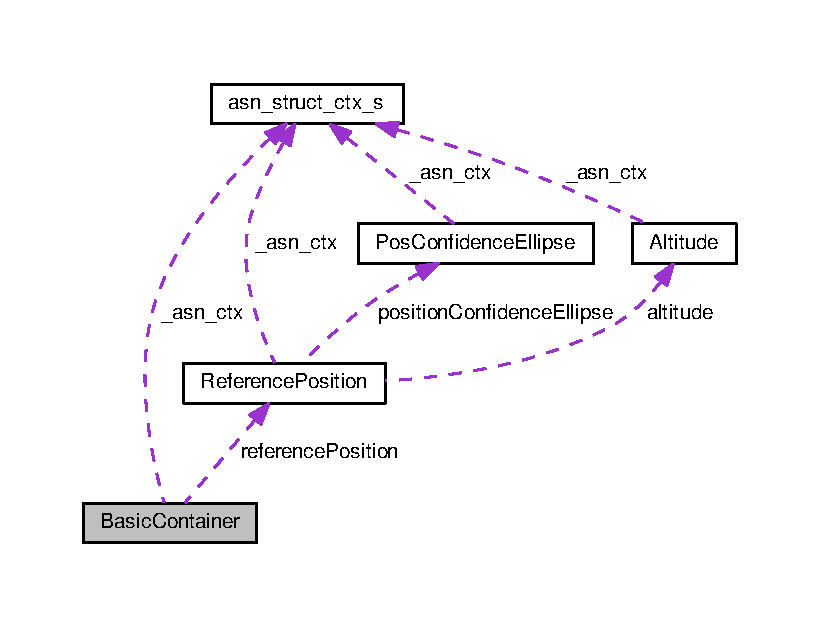
\includegraphics[width=350pt]{structBasicContainer__coll__graph}
\end{center}
\end{figure}
\subsection*{Public Attributes}
\begin{DoxyCompactItemize}
\item 
Station\+Type\+\_\+t {\bfseries station\+Type}\hypertarget{structBasicContainer_afc0597e3a8f70c72bca39345c3008537}{}\label{structBasicContainer_afc0597e3a8f70c72bca39345c3008537}

\item 
\hyperlink{structReferencePosition}{Reference\+Position\+\_\+t} {\bfseries reference\+Position}\hypertarget{structBasicContainer_a76c4c4810265ec06ca9866c64b5f5ba4}{}\label{structBasicContainer_a76c4c4810265ec06ca9866c64b5f5ba4}

\item 
\hyperlink{structasn__struct__ctx__s}{asn\+\_\+struct\+\_\+ctx\+\_\+t} {\bfseries \+\_\+asn\+\_\+ctx}\hypertarget{structBasicContainer_ad3ffaecb45f105d60285772e369770c4}{}\label{structBasicContainer_ad3ffaecb45f105d60285772e369770c4}

\end{DoxyCompactItemize}


The documentation for this struct was generated from the following file\+:\begin{DoxyCompactItemize}
\item 
include/aimsun\+\_\+extensions/\+V2\+X\+Framework/\+I\+T\+S-\/spec/Basic\+Container.\+h\end{DoxyCompactItemize}

\hypertarget{structBasicVehicleContainerHighFrequency}{}\section{Basic\+Vehicle\+Container\+High\+Frequency Struct Reference}
\label{structBasicVehicleContainerHighFrequency}\index{Basic\+Vehicle\+Container\+High\+Frequency@{Basic\+Vehicle\+Container\+High\+Frequency}}


Collaboration diagram for Basic\+Vehicle\+Container\+High\+Frequency\+:\nopagebreak
\begin{figure}[H]
\begin{center}
\leavevmode
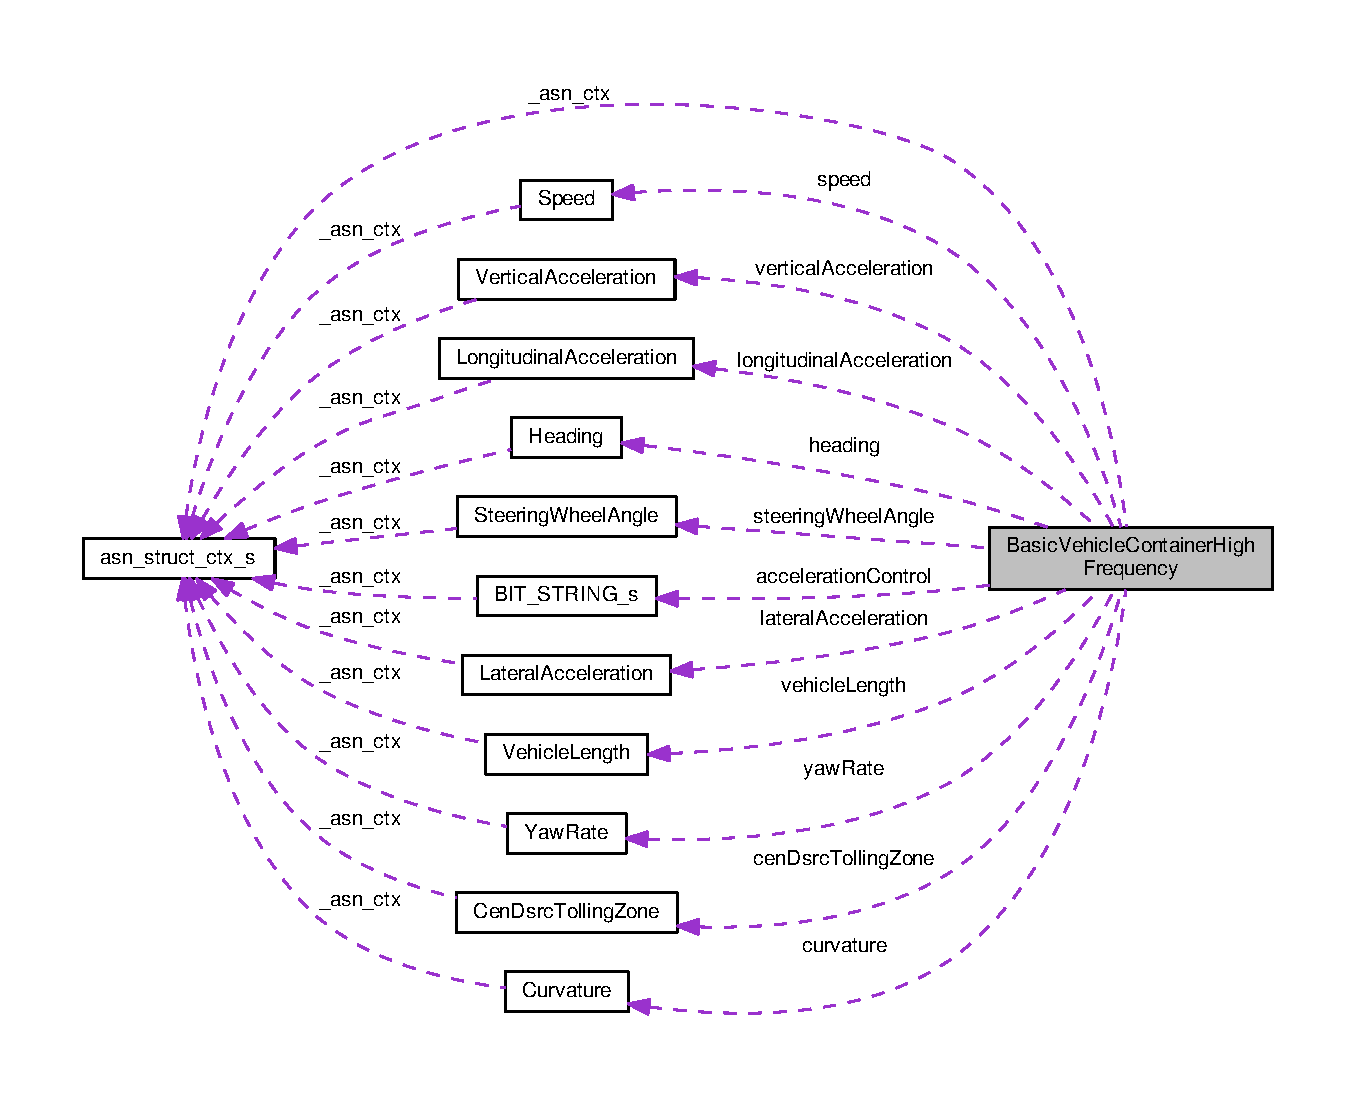
\includegraphics[width=350pt]{structBasicVehicleContainerHighFrequency__coll__graph}
\end{center}
\end{figure}
\subsection*{Public Attributes}
\begin{DoxyCompactItemize}
\item 
\hyperlink{structHeading}{Heading\+\_\+t} {\bfseries heading}\hypertarget{structBasicVehicleContainerHighFrequency_a3da2d95a6cd88f63d7659f8ce8a9444f}{}\label{structBasicVehicleContainerHighFrequency_a3da2d95a6cd88f63d7659f8ce8a9444f}

\item 
\hyperlink{structSpeed}{Speed\+\_\+t} {\bfseries speed}\hypertarget{structBasicVehicleContainerHighFrequency_aba254afa65858ceaf785a1c9ab8bd4c7}{}\label{structBasicVehicleContainerHighFrequency_aba254afa65858ceaf785a1c9ab8bd4c7}

\item 
Drive\+Direction\+\_\+t {\bfseries drive\+Direction}\hypertarget{structBasicVehicleContainerHighFrequency_a8094077edb36bab43152dacdadb789cb}{}\label{structBasicVehicleContainerHighFrequency_a8094077edb36bab43152dacdadb789cb}

\item 
\hyperlink{structVehicleLength}{Vehicle\+Length\+\_\+t} {\bfseries vehicle\+Length}\hypertarget{structBasicVehicleContainerHighFrequency_a8094aa684c8b1f7d0d59a3acd94301a4}{}\label{structBasicVehicleContainerHighFrequency_a8094aa684c8b1f7d0d59a3acd94301a4}

\item 
Vehicle\+Width\+\_\+t {\bfseries vehicle\+Width}\hypertarget{structBasicVehicleContainerHighFrequency_a078bd17b5087962c789970dca93bc73d}{}\label{structBasicVehicleContainerHighFrequency_a078bd17b5087962c789970dca93bc73d}

\item 
\hyperlink{structLongitudinalAcceleration}{Longitudinal\+Acceleration\+\_\+t} {\bfseries longitudinal\+Acceleration}\hypertarget{structBasicVehicleContainerHighFrequency_a0d7ab4f2c4dde60ed24367b76730efcd}{}\label{structBasicVehicleContainerHighFrequency_a0d7ab4f2c4dde60ed24367b76730efcd}

\item 
\hyperlink{structCurvature}{Curvature\+\_\+t} {\bfseries curvature}\hypertarget{structBasicVehicleContainerHighFrequency_ab810922ffb3fb3df1f53a0fe46c56be7}{}\label{structBasicVehicleContainerHighFrequency_ab810922ffb3fb3df1f53a0fe46c56be7}

\item 
Curvature\+Calculation\+Mode\+\_\+t {\bfseries curvature\+Calculation\+Mode}\hypertarget{structBasicVehicleContainerHighFrequency_a7a94f0e7628f7f7e73b8596ac8570c60}{}\label{structBasicVehicleContainerHighFrequency_a7a94f0e7628f7f7e73b8596ac8570c60}

\item 
\hyperlink{structYawRate}{Yaw\+Rate\+\_\+t} {\bfseries yaw\+Rate}\hypertarget{structBasicVehicleContainerHighFrequency_a74bfae5a827974b9497574ea1eee0b52}{}\label{structBasicVehicleContainerHighFrequency_a74bfae5a827974b9497574ea1eee0b52}

\item 
\hyperlink{structBIT__STRING__s}{Acceleration\+Control\+\_\+t} $\ast$ {\bfseries acceleration\+Control}\hypertarget{structBasicVehicleContainerHighFrequency_a7fdb088a6047e76d4bd71859ca8239a8}{}\label{structBasicVehicleContainerHighFrequency_a7fdb088a6047e76d4bd71859ca8239a8}

\item 
Lane\+Position\+\_\+t $\ast$ {\bfseries lane\+Position}\hypertarget{structBasicVehicleContainerHighFrequency_a2be24dbba9b67e5f13b0fca3cfb220ec}{}\label{structBasicVehicleContainerHighFrequency_a2be24dbba9b67e5f13b0fca3cfb220ec}

\item 
struct \hyperlink{structSteeringWheelAngle}{Steering\+Wheel\+Angle} $\ast$ {\bfseries steering\+Wheel\+Angle}\hypertarget{structBasicVehicleContainerHighFrequency_ac85aa45703e0b34dac7d2f083003c6e8}{}\label{structBasicVehicleContainerHighFrequency_ac85aa45703e0b34dac7d2f083003c6e8}

\item 
struct \hyperlink{structLateralAcceleration}{Lateral\+Acceleration} $\ast$ {\bfseries lateral\+Acceleration}\hypertarget{structBasicVehicleContainerHighFrequency_a5d0f1f7b5f49bff4fad98b482c730208}{}\label{structBasicVehicleContainerHighFrequency_a5d0f1f7b5f49bff4fad98b482c730208}

\item 
struct \hyperlink{structVerticalAcceleration}{Vertical\+Acceleration} $\ast$ {\bfseries vertical\+Acceleration}\hypertarget{structBasicVehicleContainerHighFrequency_a206a6024b6be92e65e9e282ae328e143}{}\label{structBasicVehicleContainerHighFrequency_a206a6024b6be92e65e9e282ae328e143}

\item 
Performance\+Class\+\_\+t $\ast$ {\bfseries performance\+Class}\hypertarget{structBasicVehicleContainerHighFrequency_af93a069de086900c2a8ac6ea6d935073}{}\label{structBasicVehicleContainerHighFrequency_af93a069de086900c2a8ac6ea6d935073}

\item 
struct \hyperlink{structCenDsrcTollingZone}{Cen\+Dsrc\+Tolling\+Zone} $\ast$ {\bfseries cen\+Dsrc\+Tolling\+Zone}\hypertarget{structBasicVehicleContainerHighFrequency_ace1b9d8c7d6712b68e47c2d62c5ce005}{}\label{structBasicVehicleContainerHighFrequency_ace1b9d8c7d6712b68e47c2d62c5ce005}

\item 
\hyperlink{structasn__struct__ctx__s}{asn\+\_\+struct\+\_\+ctx\+\_\+t} {\bfseries \+\_\+asn\+\_\+ctx}\hypertarget{structBasicVehicleContainerHighFrequency_af728d311e2391351244ee6f2f5eece14}{}\label{structBasicVehicleContainerHighFrequency_af728d311e2391351244ee6f2f5eece14}

\end{DoxyCompactItemize}


The documentation for this struct was generated from the following file\+:\begin{DoxyCompactItemize}
\item 
include/aimsun\+\_\+extensions/\+V2\+X\+Framework/\+I\+T\+S-\/spec/Basic\+Vehicle\+Container\+High\+Frequency.\+h\end{DoxyCompactItemize}

\hypertarget{structBasicVehicleContainerLowFrequency}{}\section{Basic\+Vehicle\+Container\+Low\+Frequency Struct Reference}
\label{structBasicVehicleContainerLowFrequency}\index{Basic\+Vehicle\+Container\+Low\+Frequency@{Basic\+Vehicle\+Container\+Low\+Frequency}}


Collaboration diagram for Basic\+Vehicle\+Container\+Low\+Frequency\+:\nopagebreak
\begin{figure}[H]
\begin{center}
\leavevmode
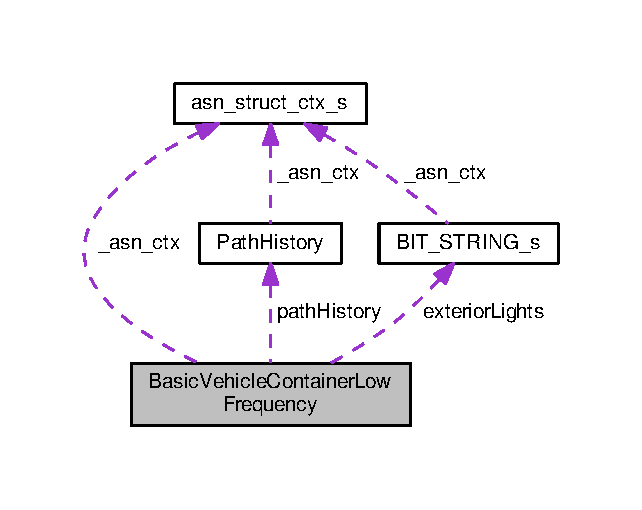
\includegraphics[width=308pt]{structBasicVehicleContainerLowFrequency__coll__graph}
\end{center}
\end{figure}
\subsection*{Public Attributes}
\begin{DoxyCompactItemize}
\item 
Vehicle\+Role\+\_\+t {\bfseries vehicle\+Role}\hypertarget{structBasicVehicleContainerLowFrequency_ab6fbbd2f872985220090a8fd0100925b}{}\label{structBasicVehicleContainerLowFrequency_ab6fbbd2f872985220090a8fd0100925b}

\item 
\hyperlink{structBIT__STRING__s}{Exterior\+Lights\+\_\+t} {\bfseries exterior\+Lights}\hypertarget{structBasicVehicleContainerLowFrequency_a1060a051709e86bc2d7af700b18a2591}{}\label{structBasicVehicleContainerLowFrequency_a1060a051709e86bc2d7af700b18a2591}

\item 
\hyperlink{structPathHistory}{Path\+History\+\_\+t} {\bfseries path\+History}\hypertarget{structBasicVehicleContainerLowFrequency_aa4c575d2af16af6995abf77f02c8d4c8}{}\label{structBasicVehicleContainerLowFrequency_aa4c575d2af16af6995abf77f02c8d4c8}

\item 
\hyperlink{structasn__struct__ctx__s}{asn\+\_\+struct\+\_\+ctx\+\_\+t} {\bfseries \+\_\+asn\+\_\+ctx}\hypertarget{structBasicVehicleContainerLowFrequency_a99dd00d9ea0dc6240914337704f30101}{}\label{structBasicVehicleContainerLowFrequency_a99dd00d9ea0dc6240914337704f30101}

\end{DoxyCompactItemize}


The documentation for this struct was generated from the following file\+:\begin{DoxyCompactItemize}
\item 
include/aimsun\+\_\+extensions/\+V2\+X\+Framework/\+I\+T\+S-\/spec/Basic\+Vehicle\+Container\+Low\+Frequency.\+h\end{DoxyCompactItemize}

\hypertarget{structBIT__STRING__s}{}\section{B\+I\+T\+\_\+\+S\+T\+R\+I\+N\+G\+\_\+s Struct Reference}
\label{structBIT__STRING__s}\index{B\+I\+T\+\_\+\+S\+T\+R\+I\+N\+G\+\_\+s@{B\+I\+T\+\_\+\+S\+T\+R\+I\+N\+G\+\_\+s}}


Collaboration diagram for B\+I\+T\+\_\+\+S\+T\+R\+I\+N\+G\+\_\+s\+:\nopagebreak
\begin{figure}[H]
\begin{center}
\leavevmode
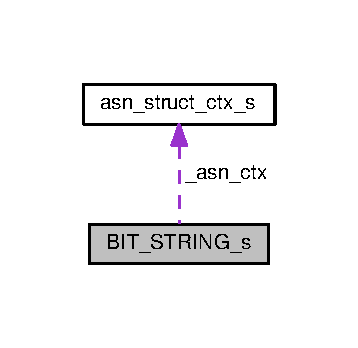
\includegraphics[width=172pt]{structBIT__STRING__s__coll__graph}
\end{center}
\end{figure}
\subsection*{Public Attributes}
\begin{DoxyCompactItemize}
\item 
uint8\+\_\+t $\ast$ {\bfseries buf}\hypertarget{structBIT__STRING__s_a0d46e66677df62aa11e24bda6a21af0c}{}\label{structBIT__STRING__s_a0d46e66677df62aa11e24bda6a21af0c}

\item 
int {\bfseries size}\hypertarget{structBIT__STRING__s_aeb19325975e1685c4dc3c5d63d3b788d}{}\label{structBIT__STRING__s_aeb19325975e1685c4dc3c5d63d3b788d}

\item 
int {\bfseries bits\+\_\+unused}\hypertarget{structBIT__STRING__s_a169280b5388fdd72e55d56950bedb46c}{}\label{structBIT__STRING__s_a169280b5388fdd72e55d56950bedb46c}

\item 
\hyperlink{structasn__struct__ctx__s}{asn\+\_\+struct\+\_\+ctx\+\_\+t} {\bfseries \+\_\+asn\+\_\+ctx}\hypertarget{structBIT__STRING__s_aa03d9b05132047959de41aa3acfdcabc}{}\label{structBIT__STRING__s_aa03d9b05132047959de41aa3acfdcabc}

\end{DoxyCompactItemize}


The documentation for this struct was generated from the following file\+:\begin{DoxyCompactItemize}
\item 
include/aimsun\+\_\+extensions/\+V2\+X\+Framework/\+A\+S\+N1/B\+I\+T\+\_\+\+S\+T\+R\+I\+N\+G.\+h\end{DoxyCompactItemize}

\hypertarget{structCAM}{}\section{C\+AM Struct Reference}
\label{structCAM}\index{C\+AM@{C\+AM}}


Collaboration diagram for C\+AM\+:\nopagebreak
\begin{figure}[H]
\begin{center}
\leavevmode
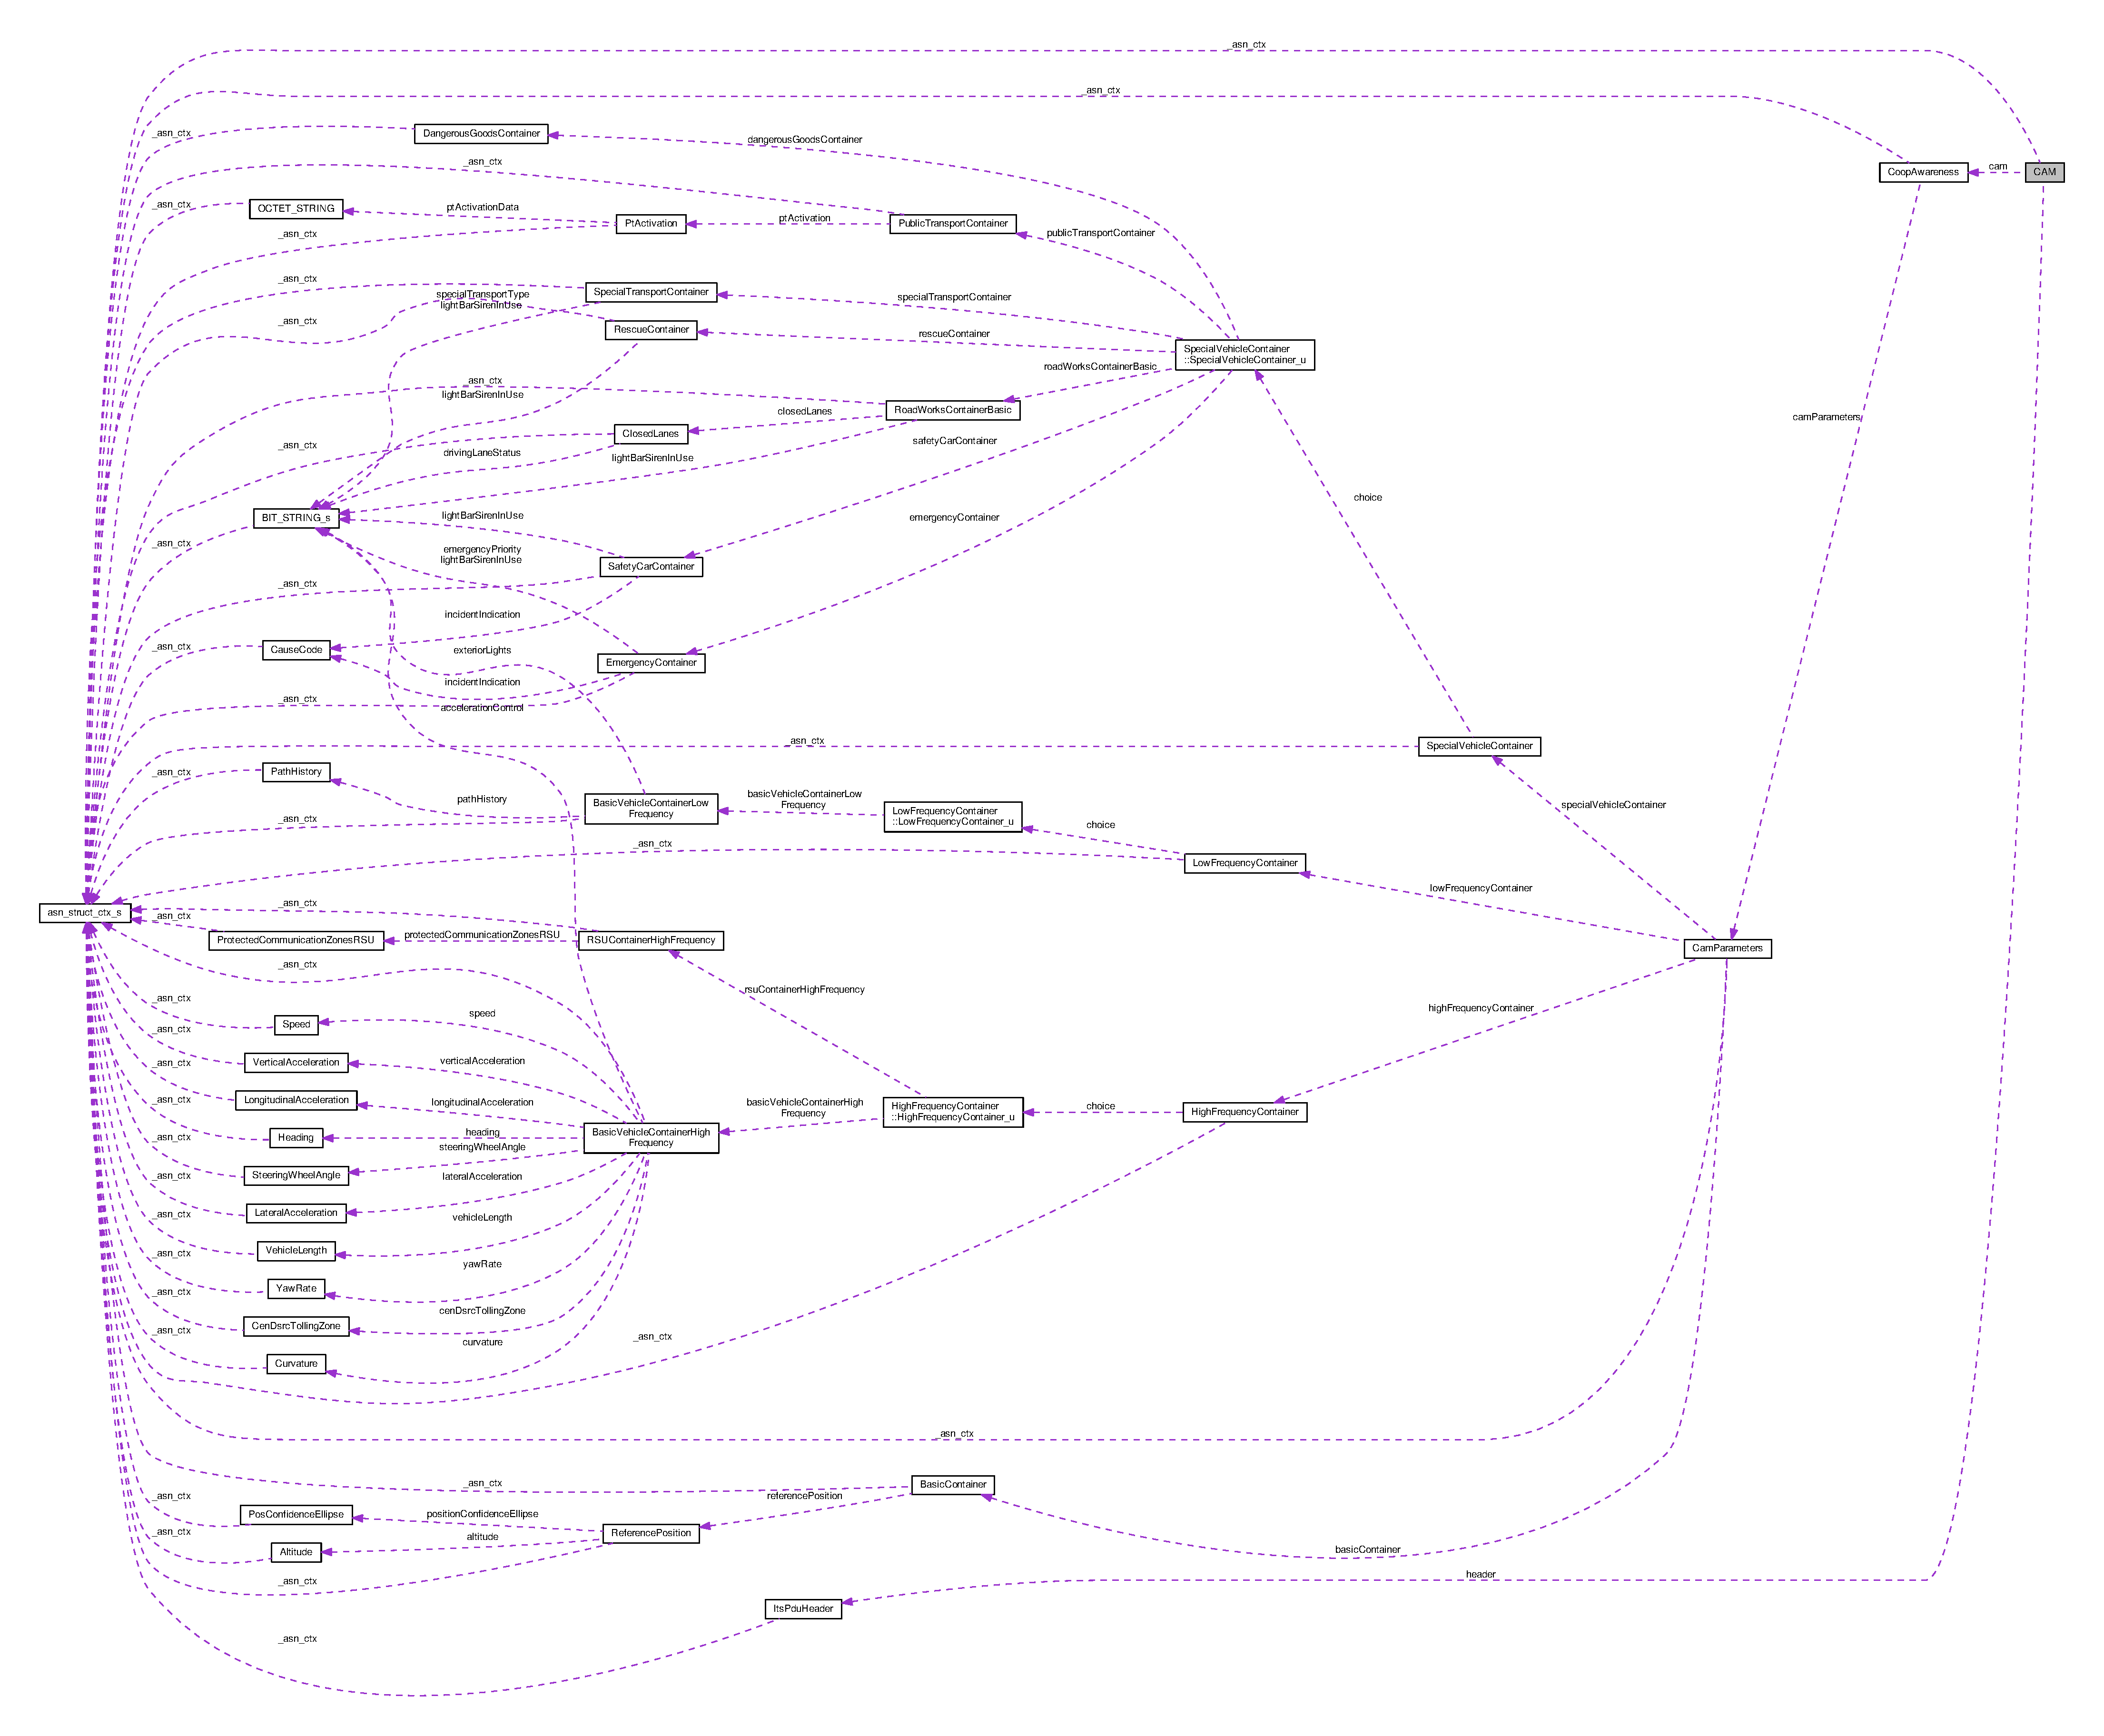
\includegraphics[width=350pt]{structCAM__coll__graph}
\end{center}
\end{figure}
\subsection*{Public Attributes}
\begin{DoxyCompactItemize}
\item 
\hyperlink{structItsPduHeader}{Its\+Pdu\+Header\+\_\+t} {\bfseries header}\hypertarget{structCAM_a60ca0b2943abd8d178d653e4ea55f96c}{}\label{structCAM_a60ca0b2943abd8d178d653e4ea55f96c}

\item 
\hyperlink{structCoopAwareness}{Coop\+Awareness\+\_\+t} {\bfseries cam}\hypertarget{structCAM_a3f337fb5369305daf9f0807f818635fc}{}\label{structCAM_a3f337fb5369305daf9f0807f818635fc}

\item 
\hyperlink{structasn__struct__ctx__s}{asn\+\_\+struct\+\_\+ctx\+\_\+t} {\bfseries \+\_\+asn\+\_\+ctx}\hypertarget{structCAM_a195d8b3b3cfb090f4de190072eeaaf09}{}\label{structCAM_a195d8b3b3cfb090f4de190072eeaaf09}

\end{DoxyCompactItemize}


The documentation for this struct was generated from the following file\+:\begin{DoxyCompactItemize}
\item 
include/aimsun\+\_\+extensions/\+V2\+X\+Framework/\+I\+T\+S-\/spec/C\+A\+M.\+h\end{DoxyCompactItemize}

\hypertarget{classCAMMessage}{}\section{C\+A\+M\+Message Class Reference}
\label{classCAMMessage}\index{C\+A\+M\+Message@{C\+A\+M\+Message}}


A \hyperlink{structCAM}{C\+AM} message.  




{\ttfamily \#include $<$C\+A\+M\+Message.\+h$>$}



Inheritance diagram for C\+A\+M\+Message\+:\nopagebreak
\begin{figure}[H]
\begin{center}
\leavevmode
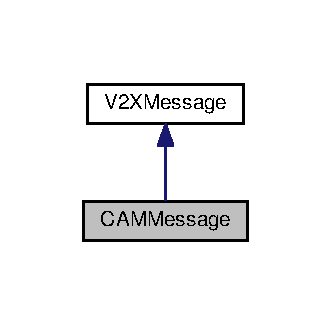
\includegraphics[width=159pt]{classCAMMessage__inherit__graph}
\end{center}
\end{figure}


Collaboration diagram for C\+A\+M\+Message\+:\nopagebreak
\begin{figure}[H]
\begin{center}
\leavevmode
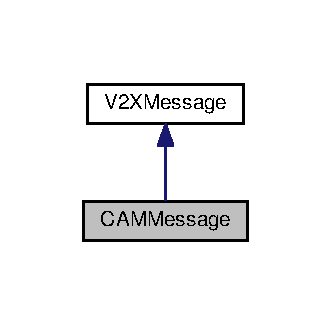
\includegraphics[width=159pt]{classCAMMessage__coll__graph}
\end{center}
\end{figure}
\subsection*{Public Member Functions}
\begin{DoxyCompactItemize}
\item 
\hyperlink{classCAMMessage_a5afb86a939afcd5c384510bc882fb39a}{C\+A\+M\+Message} ()\hypertarget{classCAMMessage_a5afb86a939afcd5c384510bc882fb39a}{}\label{classCAMMessage_a5afb86a939afcd5c384510bc882fb39a}

\begin{DoxyCompactList}\small\item\em \hyperlink{classCAMMessage}{C\+A\+M\+Message} constructor. \end{DoxyCompactList}\item 
\hyperlink{classCAMMessage_aa98df842a81887dd737edd6f8d987a59}{C\+A\+M\+Message} (const \hyperlink{classCAMMessage}{C\+A\+M\+Message} \&other)
\begin{DoxyCompactList}\small\item\em \hyperlink{classCAMMessage}{C\+A\+M\+Message} copy constructor. \end{DoxyCompactList}\item 
virtual \hyperlink{classCAMMessage_a2bc3fbfcf7ff6808a864e67d9fbc3105}{$\sim$\+C\+A\+M\+Message} ()\hypertarget{classCAMMessage_a2bc3fbfcf7ff6808a864e67d9fbc3105}{}\label{classCAMMessage_a2bc3fbfcf7ff6808a864e67d9fbc3105}

\begin{DoxyCompactList}\small\item\em Deconstructor. \end{DoxyCompactList}\item 
virtual \hyperlink{classV2XMessage}{V2\+X\+Message} $\ast$ \hyperlink{classCAMMessage_a27935907b25d9e8648891a281dd48df6}{copy} () const 
\begin{DoxyCompactList}\small\item\em Copy the message content (shallow copy) \end{DoxyCompactList}\item 
virtual void \hyperlink{classCAMMessage_ae2b5d2a030f6a6d6580c900ee4c38db5}{print} () const \hypertarget{classCAMMessage_ae2b5d2a030f6a6d6580c900ee4c38db5}{}\label{classCAMMessage_ae2b5d2a030f6a6d6580c900ee4c38db5}

\begin{DoxyCompactList}\small\item\em print the message over console in X\+ML format \end{DoxyCompactList}\item 
virtual quint32 \hyperlink{classCAMMessage_ace1b6d647755a20130e692565882ce68}{get\+Size} () const 
\begin{DoxyCompactList}\small\item\em get the size of a message \end{DoxyCompactList}\item 
bool \hyperlink{classCAMMessage_a71ab26737e4f5163bae6d0f14c18eb5c}{from\+X\+ML} (const char $\ast$buf, size\+\_\+t size)
\begin{DoxyCompactList}\small\item\em Build this object from an X\+ML representation. \end{DoxyCompactList}\item 
bool \hyperlink{classCAMMessage_a99fd5af2f59521832d50b2191aee405a}{from\+X\+ML} (const char $\ast$filename)
\begin{DoxyCompactList}\small\item\em Build this object from a file containing an X\+ML representation. \end{DoxyCompactList}\item 
bool \hyperlink{classCAMMessage_abc5174be6c558073d15dd0f1bb395099}{to\+X\+ML} (std\+::ostream $\ast$out) const 
\begin{DoxyCompactList}\small\item\em Write this message in an X\+ML format. \end{DoxyCompactList}\item 
void \hyperlink{classCAMMessage_ade4591ace41f3dd40f65e7c34cd82cab}{to\+Console} () const \hypertarget{classCAMMessage_ade4591ace41f3dd40f65e7c34cd82cab}{}\label{classCAMMessage_ade4591ace41f3dd40f65e7c34cd82cab}

\begin{DoxyCompactList}\small\item\em Print the message to the console. \end{DoxyCompactList}\item 
const \hyperlink{structCAM}{C\+A\+M\+\_\+t} $\ast$ \hyperlink{classCAMMessage_abe838f3849dddd612f257d073ed0ceab}{const\+Data} () const 
\begin{DoxyCompactList}\small\item\em Read-\/only data access. \end{DoxyCompactList}\item 
\hyperlink{structCAM}{C\+A\+M\+\_\+t} $\ast$ \hyperlink{classCAMMessage_af92e259fc9a18a36a16ed692c1546f47}{data} ()
\begin{DoxyCompactList}\small\item\em data Write data access \end{DoxyCompactList}\item 
void \hyperlink{classCAMMessage_abd793880c42373a626d9032187d1facf}{initialize\+Empty} ()\hypertarget{classCAMMessage_abd793880c42373a626d9032187d1facf}{}\label{classCAMMessage_abd793880c42373a626d9032187d1facf}

\begin{DoxyCompactList}\small\item\em Allocate raw data for directly manipulating it. \end{DoxyCompactList}\end{DoxyCompactItemize}


\subsection{Detailed Description}
A \hyperlink{structCAM}{C\+AM} message. 

Copyright T\+SS 2017

Author\+: Natale Patriciello \href{mailto:natale.patriciello@aimsun.com}{\tt natale.\+patriciello@aimsun.\+com}

Represents a \hyperlink{structCAM}{C\+AM} Message through the use of \hyperlink{classASN1CContainer}{A\+S\+N1\+C\+Container}. 

\subsection{Constructor \& Destructor Documentation}
\index{C\+A\+M\+Message@{C\+A\+M\+Message}!C\+A\+M\+Message@{C\+A\+M\+Message}}
\index{C\+A\+M\+Message@{C\+A\+M\+Message}!C\+A\+M\+Message@{C\+A\+M\+Message}}
\subsubsection[{\texorpdfstring{C\+A\+M\+Message(const C\+A\+M\+Message \&other)}{CAMMessage(const CAMMessage &other)}}]{\setlength{\rightskip}{0pt plus 5cm}C\+A\+M\+Message\+::\+C\+A\+M\+Message (
\begin{DoxyParamCaption}
\item[{const {\bf C\+A\+M\+Message} \&}]{other}
\end{DoxyParamCaption}
)}\hypertarget{classCAMMessage_aa98df842a81887dd737edd6f8d987a59}{}\label{classCAMMessage_aa98df842a81887dd737edd6f8d987a59}


\hyperlink{classCAMMessage}{C\+A\+M\+Message} copy constructor. 


\begin{DoxyParams}{Parameters}
{\em other} & the copy \\
\hline
\end{DoxyParams}


\subsection{Member Function Documentation}
\index{C\+A\+M\+Message@{C\+A\+M\+Message}!const\+Data@{const\+Data}}
\index{const\+Data@{const\+Data}!C\+A\+M\+Message@{C\+A\+M\+Message}}
\subsubsection[{\texorpdfstring{const\+Data() const }{constData() const }}]{\setlength{\rightskip}{0pt plus 5cm}const {\bf C\+A\+M\+\_\+t}$\ast$ C\+A\+M\+Message\+::const\+Data (
\begin{DoxyParamCaption}
{}
\end{DoxyParamCaption}
) const}\hypertarget{classCAMMessage_abe838f3849dddd612f257d073ed0ceab}{}\label{classCAMMessage_abe838f3849dddd612f257d073ed0ceab}


Read-\/only data access. 

\begin{DoxyReturn}{Returns}
A copy of the data 
\end{DoxyReturn}
\index{C\+A\+M\+Message@{C\+A\+M\+Message}!copy@{copy}}
\index{copy@{copy}!C\+A\+M\+Message@{C\+A\+M\+Message}}
\subsubsection[{\texorpdfstring{copy() const }{copy() const }}]{\setlength{\rightskip}{0pt plus 5cm}virtual {\bf V2\+X\+Message}$\ast$ C\+A\+M\+Message\+::copy (
\begin{DoxyParamCaption}
{}
\end{DoxyParamCaption}
) const\hspace{0.3cm}{\ttfamily [virtual]}}\hypertarget{classCAMMessage_a27935907b25d9e8648891a281dd48df6}{}\label{classCAMMessage_a27935907b25d9e8648891a281dd48df6}


Copy the message content (shallow copy) 

\begin{DoxyReturn}{Returns}
a copy of the message 
\end{DoxyReturn}


Implements \hyperlink{classV2XMessage_a0838dc7505794641df7f0a3bdc4148b1}{V2\+X\+Message}.

\index{C\+A\+M\+Message@{C\+A\+M\+Message}!data@{data}}
\index{data@{data}!C\+A\+M\+Message@{C\+A\+M\+Message}}
\subsubsection[{\texorpdfstring{data()}{data()}}]{\setlength{\rightskip}{0pt plus 5cm}{\bf C\+A\+M\+\_\+t}$\ast$ C\+A\+M\+Message\+::data (
\begin{DoxyParamCaption}
{}
\end{DoxyParamCaption}
)}\hypertarget{classCAMMessage_af92e259fc9a18a36a16ed692c1546f47}{}\label{classCAMMessage_af92e259fc9a18a36a16ed692c1546f47}


data Write data access 

\begin{DoxyReturn}{Returns}
A copy of the data 
\end{DoxyReturn}
\index{C\+A\+M\+Message@{C\+A\+M\+Message}!from\+X\+ML@{from\+X\+ML}}
\index{from\+X\+ML@{from\+X\+ML}!C\+A\+M\+Message@{C\+A\+M\+Message}}
\subsubsection[{\texorpdfstring{from\+X\+M\+L(const char $\ast$buf, size\+\_\+t size)}{fromXML(const char *buf, size_t size)}}]{\setlength{\rightskip}{0pt plus 5cm}bool C\+A\+M\+Message\+::from\+X\+ML (
\begin{DoxyParamCaption}
\item[{const char $\ast$}]{buf, }
\item[{size\+\_\+t}]{size}
\end{DoxyParamCaption}
)}\hypertarget{classCAMMessage_a71ab26737e4f5163bae6d0f14c18eb5c}{}\label{classCAMMessage_a71ab26737e4f5163bae6d0f14c18eb5c}


Build this object from an X\+ML representation. 


\begin{DoxyParams}{Parameters}
{\em buf} & buffer of the representation \\
\hline
{\em size} & size of the buffer \\
\hline
\end{DoxyParams}
\begin{DoxyReturn}{Returns}
true if the construction was fine 
\end{DoxyReturn}
\index{C\+A\+M\+Message@{C\+A\+M\+Message}!from\+X\+ML@{from\+X\+ML}}
\index{from\+X\+ML@{from\+X\+ML}!C\+A\+M\+Message@{C\+A\+M\+Message}}
\subsubsection[{\texorpdfstring{from\+X\+M\+L(const char $\ast$filename)}{fromXML(const char *filename)}}]{\setlength{\rightskip}{0pt plus 5cm}bool C\+A\+M\+Message\+::from\+X\+ML (
\begin{DoxyParamCaption}
\item[{const char $\ast$}]{filename}
\end{DoxyParamCaption}
)}\hypertarget{classCAMMessage_a99fd5af2f59521832d50b2191aee405a}{}\label{classCAMMessage_a99fd5af2f59521832d50b2191aee405a}


Build this object from a file containing an X\+ML representation. 


\begin{DoxyParams}{Parameters}
{\em filename} & File name \\
\hline
\end{DoxyParams}
\begin{DoxyReturn}{Returns}
true if the construction was fine 
\end{DoxyReturn}
\index{C\+A\+M\+Message@{C\+A\+M\+Message}!get\+Size@{get\+Size}}
\index{get\+Size@{get\+Size}!C\+A\+M\+Message@{C\+A\+M\+Message}}
\subsubsection[{\texorpdfstring{get\+Size() const }{getSize() const }}]{\setlength{\rightskip}{0pt plus 5cm}virtual quint32 C\+A\+M\+Message\+::get\+Size (
\begin{DoxyParamCaption}
{}
\end{DoxyParamCaption}
) const\hspace{0.3cm}{\ttfamily [virtual]}}\hypertarget{classCAMMessage_ace1b6d647755a20130e692565882ce68}{}\label{classCAMMessage_ace1b6d647755a20130e692565882ce68}


get the size of a message 

\begin{DoxyReturn}{Returns}
the size of a message 
\end{DoxyReturn}


Implements \hyperlink{classV2XMessage_ae1b54af9f8f88bb0c2a6967d3f6e7777}{V2\+X\+Message}.

\index{C\+A\+M\+Message@{C\+A\+M\+Message}!to\+X\+ML@{to\+X\+ML}}
\index{to\+X\+ML@{to\+X\+ML}!C\+A\+M\+Message@{C\+A\+M\+Message}}
\subsubsection[{\texorpdfstring{to\+X\+M\+L(std\+::ostream $\ast$out) const }{toXML(std::ostream *out) const }}]{\setlength{\rightskip}{0pt plus 5cm}bool C\+A\+M\+Message\+::to\+X\+ML (
\begin{DoxyParamCaption}
\item[{std\+::ostream $\ast$}]{out}
\end{DoxyParamCaption}
) const}\hypertarget{classCAMMessage_abc5174be6c558073d15dd0f1bb395099}{}\label{classCAMMessage_abc5174be6c558073d15dd0f1bb395099}


Write this message in an X\+ML format. 


\begin{DoxyParams}{Parameters}
{\em out} & output stream \\
\hline
\end{DoxyParams}
\begin{DoxyReturn}{Returns}
true if everything went fine 
\end{DoxyReturn}


The documentation for this class was generated from the following file\+:\begin{DoxyCompactItemize}
\item 
include/aimsun\+\_\+extensions/\+V2\+X\+Framework/C\+A\+M\+Message.\+h\end{DoxyCompactItemize}

\hypertarget{structCamParameters}{}\section{Cam\+Parameters Struct Reference}
\label{structCamParameters}\index{Cam\+Parameters@{Cam\+Parameters}}


Collaboration diagram for Cam\+Parameters\+:\nopagebreak
\begin{figure}[H]
\begin{center}
\leavevmode
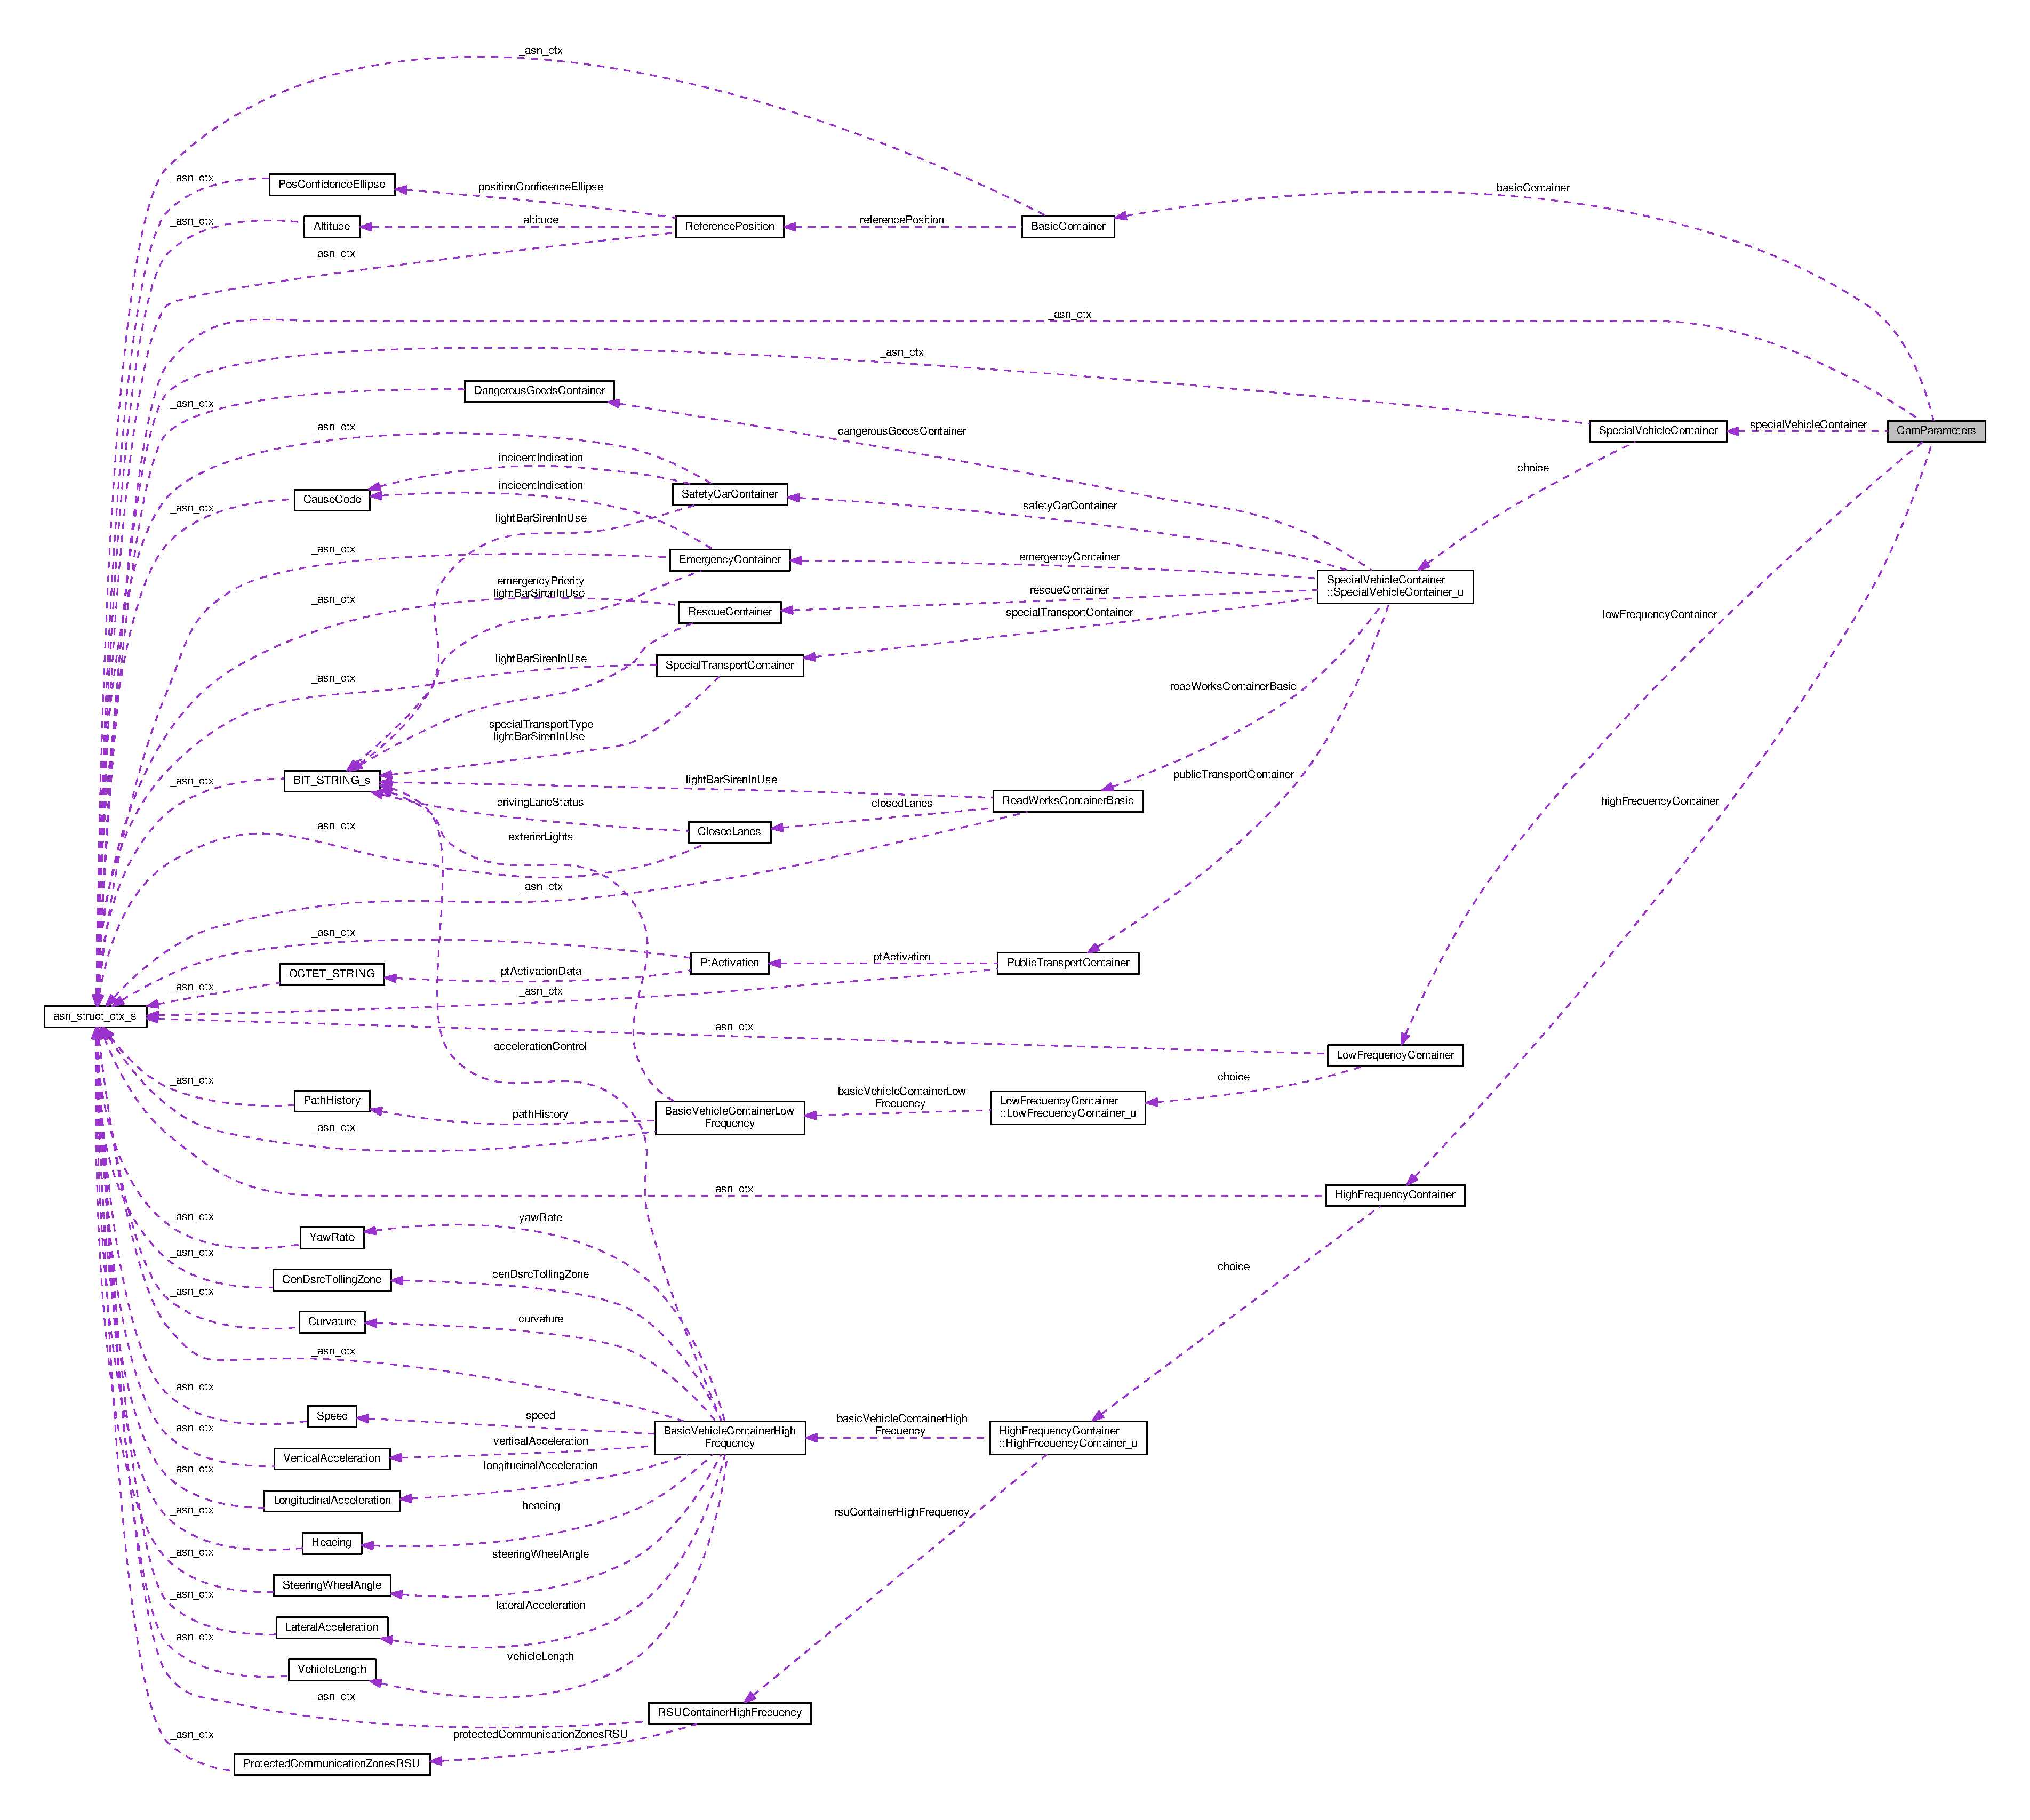
\includegraphics[width=350pt]{structCamParameters__coll__graph}
\end{center}
\end{figure}
\subsection*{Public Attributes}
\begin{DoxyCompactItemize}
\item 
\hyperlink{structBasicContainer}{Basic\+Container\+\_\+t} {\bfseries basic\+Container}\hypertarget{structCamParameters_a818dbf58f693aa87ef21da329ad3de05}{}\label{structCamParameters_a818dbf58f693aa87ef21da329ad3de05}

\item 
\hyperlink{structHighFrequencyContainer}{High\+Frequency\+Container\+\_\+t} {\bfseries high\+Frequency\+Container}\hypertarget{structCamParameters_af3c191d54d4daaf946cebe004e675a97}{}\label{structCamParameters_af3c191d54d4daaf946cebe004e675a97}

\item 
struct \hyperlink{structLowFrequencyContainer}{Low\+Frequency\+Container} $\ast$ {\bfseries low\+Frequency\+Container}\hypertarget{structCamParameters_ab58322b63b8c3a3119f1e9124ceef5aa}{}\label{structCamParameters_ab58322b63b8c3a3119f1e9124ceef5aa}

\item 
struct \hyperlink{structSpecialVehicleContainer}{Special\+Vehicle\+Container} $\ast$ {\bfseries special\+Vehicle\+Container}\hypertarget{structCamParameters_ae2d6b6e8ff683a6f7095762f78da115d}{}\label{structCamParameters_ae2d6b6e8ff683a6f7095762f78da115d}

\item 
\hyperlink{structasn__struct__ctx__s}{asn\+\_\+struct\+\_\+ctx\+\_\+t} {\bfseries \+\_\+asn\+\_\+ctx}\hypertarget{structCamParameters_a69deb9c653f4a600c075f735dce1e96a}{}\label{structCamParameters_a69deb9c653f4a600c075f735dce1e96a}

\end{DoxyCompactItemize}


The documentation for this struct was generated from the following file\+:\begin{DoxyCompactItemize}
\item 
include/aimsun\+\_\+extensions/\+V2\+X\+Framework/\+I\+T\+S-\/spec/Cam\+Parameters.\+h\end{DoxyCompactItemize}

\hypertarget{structCauseCode}{}\section{Cause\+Code Struct Reference}
\label{structCauseCode}\index{Cause\+Code@{Cause\+Code}}


Collaboration diagram for Cause\+Code\+:\nopagebreak
\begin{figure}[H]
\begin{center}
\leavevmode
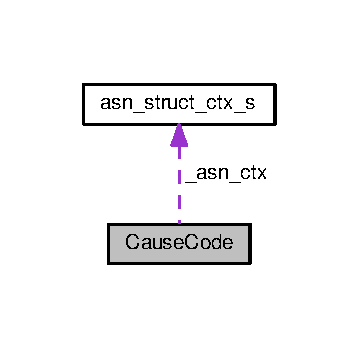
\includegraphics[width=172pt]{structCauseCode__coll__graph}
\end{center}
\end{figure}
\subsection*{Public Attributes}
\begin{DoxyCompactItemize}
\item 
Cause\+Code\+Type\+\_\+t {\bfseries cause\+Code}\hypertarget{structCauseCode_acb66d21175aa9a9ebf439c7a83d0832d}{}\label{structCauseCode_acb66d21175aa9a9ebf439c7a83d0832d}

\item 
Sub\+Cause\+Code\+Type\+\_\+t {\bfseries sub\+Cause\+Code}\hypertarget{structCauseCode_afc5fdd06b09bc244a6f5e8c2034f24ff}{}\label{structCauseCode_afc5fdd06b09bc244a6f5e8c2034f24ff}

\item 
\hyperlink{structasn__struct__ctx__s}{asn\+\_\+struct\+\_\+ctx\+\_\+t} {\bfseries \+\_\+asn\+\_\+ctx}\hypertarget{structCauseCode_a6d154f1bd07ba07f0904218aacc18762}{}\label{structCauseCode_a6d154f1bd07ba07f0904218aacc18762}

\end{DoxyCompactItemize}


The documentation for this struct was generated from the following file\+:\begin{DoxyCompactItemize}
\item 
include/aimsun\+\_\+extensions/\+V2\+X\+Framework/\+I\+T\+S-\/spec/Cause\+Code.\+h\end{DoxyCompactItemize}

\hypertarget{structCenDsrcTollingZone}{}\section{Cen\+Dsrc\+Tolling\+Zone Struct Reference}
\label{structCenDsrcTollingZone}\index{Cen\+Dsrc\+Tolling\+Zone@{Cen\+Dsrc\+Tolling\+Zone}}


Collaboration diagram for Cen\+Dsrc\+Tolling\+Zone\+:\nopagebreak
\begin{figure}[H]
\begin{center}
\leavevmode
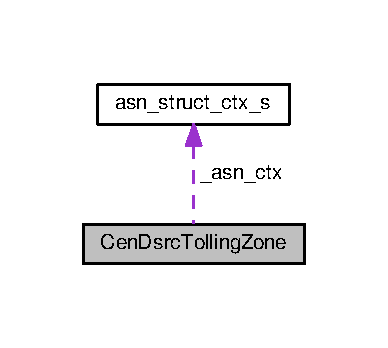
\includegraphics[width=186pt]{structCenDsrcTollingZone__coll__graph}
\end{center}
\end{figure}
\subsection*{Public Attributes}
\begin{DoxyCompactItemize}
\item 
Latitude\+\_\+t {\bfseries protected\+Zone\+Latitude}\hypertarget{structCenDsrcTollingZone_a0bbfcfeee86f98b0485a98e4c8044a89}{}\label{structCenDsrcTollingZone_a0bbfcfeee86f98b0485a98e4c8044a89}

\item 
Longitude\+\_\+t {\bfseries protected\+Zone\+Longitude}\hypertarget{structCenDsrcTollingZone_ac6fe8cc4ab012ede258f3528732ed5e2}{}\label{structCenDsrcTollingZone_ac6fe8cc4ab012ede258f3528732ed5e2}

\item 
Cen\+Dsrc\+Tolling\+Zone\+I\+D\+\_\+t $\ast$ {\bfseries cen\+Dsrc\+Tolling\+Zone\+ID}\hypertarget{structCenDsrcTollingZone_ac5b03cb1e61cb3551e8f5f6d8e516b26}{}\label{structCenDsrcTollingZone_ac5b03cb1e61cb3551e8f5f6d8e516b26}

\item 
\hyperlink{structasn__struct__ctx__s}{asn\+\_\+struct\+\_\+ctx\+\_\+t} {\bfseries \+\_\+asn\+\_\+ctx}\hypertarget{structCenDsrcTollingZone_a6f310891ae7b864d625c09a08f301d6d}{}\label{structCenDsrcTollingZone_a6f310891ae7b864d625c09a08f301d6d}

\end{DoxyCompactItemize}


The documentation for this struct was generated from the following file\+:\begin{DoxyCompactItemize}
\item 
include/aimsun\+\_\+extensions/\+V2\+X\+Framework/\+I\+T\+S-\/spec/Cen\+Dsrc\+Tolling\+Zone.\+h\end{DoxyCompactItemize}

\hypertarget{classChannel}{}\section{Channel Class Reference}
\label{classChannel}\index{Channel@{Channel}}


Abstract \hyperlink{classChannel}{Channel} Base Class.  




{\ttfamily \#include $<$Channel.\+h$>$}



Inheritance diagram for Channel\+:\nopagebreak
\begin{figure}[H]
\begin{center}
\leavevmode
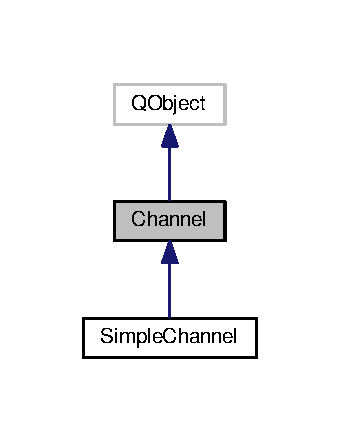
\includegraphics[width=163pt]{classChannel__inherit__graph}
\end{center}
\end{figure}


Collaboration diagram for Channel\+:\nopagebreak
\begin{figure}[H]
\begin{center}
\leavevmode
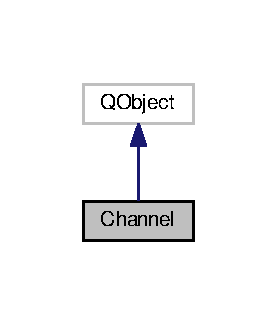
\includegraphics[width=133pt]{classChannel__coll__graph}
\end{center}
\end{figure}
\subsection*{Public Member Functions}
\begin{DoxyCompactItemize}
\item 
\hyperlink{classChannel_af2b4b16288cbb2c592b1e0f6486c2430}{Channel} ()\hypertarget{classChannel_af2b4b16288cbb2c592b1e0f6486c2430}{}\label{classChannel_af2b4b16288cbb2c592b1e0f6486c2430}

\begin{DoxyCompactList}\small\item\em \hyperlink{classChannel}{Channel} constructor. \end{DoxyCompactList}\item 
virtual \hyperlink{classChannel_af649ff0e4381291b608813b35f998047}{$\sim$\+Channel} ()\hypertarget{classChannel_af649ff0e4381291b608813b35f998047}{}\label{classChannel_af649ff0e4381291b608813b35f998047}

\begin{DoxyCompactList}\small\item\em \hyperlink{classChannel}{Channel} deconstructor. \end{DoxyCompactList}\item 
qint32 \hyperlink{classChannel_af2a456051ae4b3765e4dd01f169c0317}{get\+Id} (void) const 
\item 
virtual quint32 \hyperlink{classChannel_a28065f95665bec4b81c305dbe04d2af4}{get\+N\+Devices} (void) const =0
\end{DoxyCompactItemize}


\subsection{Detailed Description}
Abstract \hyperlink{classChannel}{Channel} Base Class. 

\begin{DoxySeeAlso}{See also}
\hyperlink{classSimpleChannel}{Simple\+Channel} 
\end{DoxySeeAlso}


\subsection{Member Function Documentation}
\index{Channel@{Channel}!get\+Id@{get\+Id}}
\index{get\+Id@{get\+Id}!Channel@{Channel}}
\subsubsection[{\texorpdfstring{get\+Id(void) const }{getId(void) const }}]{\setlength{\rightskip}{0pt plus 5cm}qint32 Channel\+::get\+Id (
\begin{DoxyParamCaption}
\item[{void}]{}
\end{DoxyParamCaption}
) const\hspace{0.3cm}{\ttfamily [inline]}}\hypertarget{classChannel_af2a456051ae4b3765e4dd01f169c0317}{}\label{classChannel_af2a456051ae4b3765e4dd01f169c0317}
\begin{DoxyReturn}{Returns}
the unique id of this channel
\end{DoxyReturn}
This unique id happens to be also the index of the \hyperlink{classChannel}{Channel} into the Channel\+List. \index{Channel@{Channel}!get\+N\+Devices@{get\+N\+Devices}}
\index{get\+N\+Devices@{get\+N\+Devices}!Channel@{Channel}}
\subsubsection[{\texorpdfstring{get\+N\+Devices(void) const =0}{getNDevices(void) const =0}}]{\setlength{\rightskip}{0pt plus 5cm}virtual quint32 Channel\+::get\+N\+Devices (
\begin{DoxyParamCaption}
\item[{void}]{}
\end{DoxyParamCaption}
) const\hspace{0.3cm}{\ttfamily [pure virtual]}}\hypertarget{classChannel_a28065f95665bec4b81c305dbe04d2af4}{}\label{classChannel_a28065f95665bec4b81c305dbe04d2af4}
\begin{DoxyReturn}{Returns}
the number of Net\+Devices connected to this \hyperlink{classChannel}{Channel}. 
\end{DoxyReturn}


Implemented in \hyperlink{classSimpleChannel_a6e2407c25fa79ff9f0a22fa1bd65f1d7}{Simple\+Channel}.



The documentation for this class was generated from the following file\+:\begin{DoxyCompactItemize}
\item 
include/aimsun\+\_\+extensions/\+V2\+X\+Framework/Channel.\+h\end{DoxyCompactItemize}

\hypertarget{structClosedLanes}{}\section{Closed\+Lanes Struct Reference}
\label{structClosedLanes}\index{Closed\+Lanes@{Closed\+Lanes}}


Collaboration diagram for Closed\+Lanes\+:\nopagebreak
\begin{figure}[H]
\begin{center}
\leavevmode
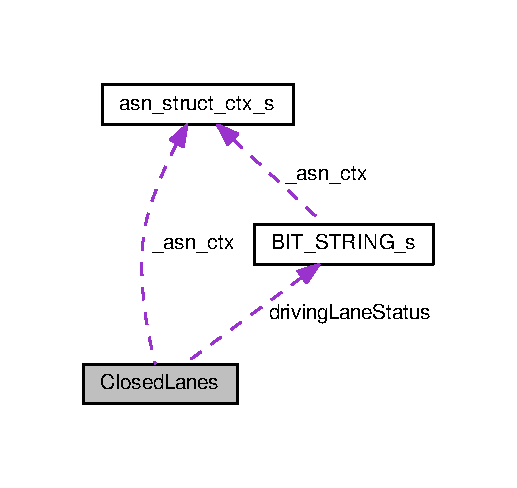
\includegraphics[width=248pt]{structClosedLanes__coll__graph}
\end{center}
\end{figure}
\subsection*{Public Attributes}
\begin{DoxyCompactItemize}
\item 
Hard\+Shoulder\+Status\+\_\+t $\ast$ {\bfseries hard\+Shoulder\+Status}\hypertarget{structClosedLanes_a20469a3710d76df3c7224573a75aeb2b}{}\label{structClosedLanes_a20469a3710d76df3c7224573a75aeb2b}

\item 
\hyperlink{structBIT__STRING__s}{Driving\+Lane\+Status\+\_\+t} {\bfseries driving\+Lane\+Status}\hypertarget{structClosedLanes_a057b7bc1606e75a52240a4b2b1505e1c}{}\label{structClosedLanes_a057b7bc1606e75a52240a4b2b1505e1c}

\item 
\hyperlink{structasn__struct__ctx__s}{asn\+\_\+struct\+\_\+ctx\+\_\+t} {\bfseries \+\_\+asn\+\_\+ctx}\hypertarget{structClosedLanes_a79b5fbe608d2500d26e17ee32b45c5a0}{}\label{structClosedLanes_a79b5fbe608d2500d26e17ee32b45c5a0}

\end{DoxyCompactItemize}


The documentation for this struct was generated from the following file\+:\begin{DoxyCompactItemize}
\item 
include/aimsun\+\_\+extensions/\+V2\+X\+Framework/\+I\+T\+S-\/spec/Closed\+Lanes.\+h\end{DoxyCompactItemize}

\hypertarget{structCompleteVehicleCharacteristics}{}\section{Complete\+Vehicle\+Characteristics Struct Reference}
\label{structCompleteVehicleCharacteristics}\index{Complete\+Vehicle\+Characteristics@{Complete\+Vehicle\+Characteristics}}


Collaboration diagram for Complete\+Vehicle\+Characteristics\+:\nopagebreak
\begin{figure}[H]
\begin{center}
\leavevmode
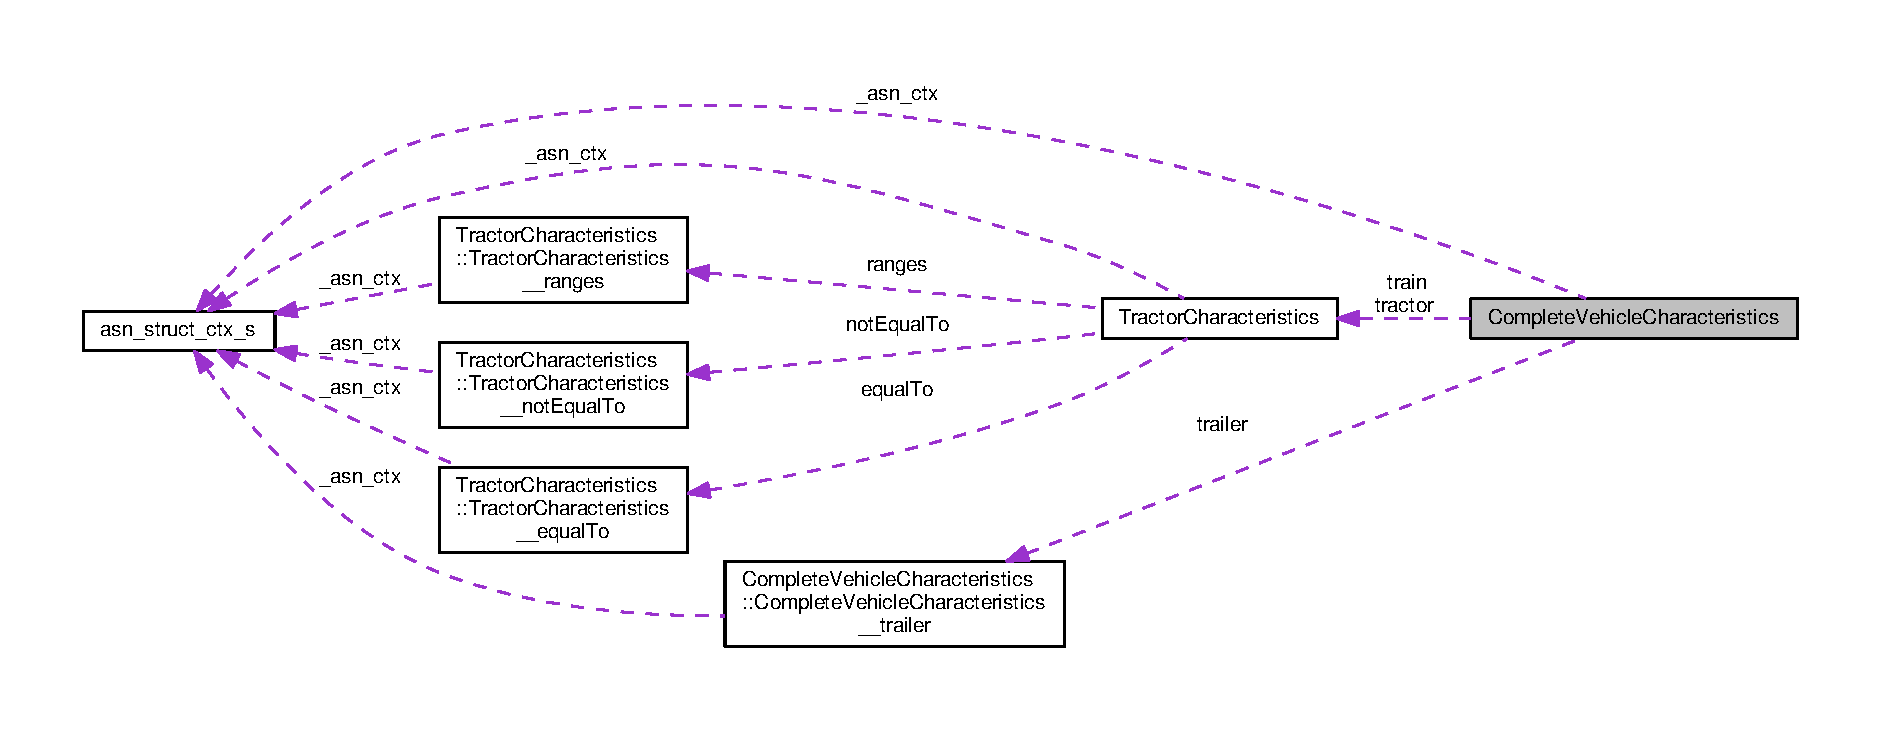
\includegraphics[width=350pt]{structCompleteVehicleCharacteristics__coll__graph}
\end{center}
\end{figure}
\subsection*{Classes}
\begin{DoxyCompactItemize}
\item 
struct \hyperlink{structCompleteVehicleCharacteristics_1_1CompleteVehicleCharacteristics____trailer}{Complete\+Vehicle\+Characteristics\+\_\+\+\_\+trailer}
\end{DoxyCompactItemize}
\subsection*{Public Attributes}
\begin{DoxyCompactItemize}
\item 
struct \hyperlink{structTractorCharacteristics}{Tractor\+Characteristics} $\ast$ {\bfseries tractor}\hypertarget{structCompleteVehicleCharacteristics_a2afb2396dca896b7ae4bb20d297b6ff2}{}\label{structCompleteVehicleCharacteristics_a2afb2396dca896b7ae4bb20d297b6ff2}

\item 
struct \hyperlink{structCompleteVehicleCharacteristics_1_1CompleteVehicleCharacteristics____trailer}{Complete\+Vehicle\+Characteristics\+::\+Complete\+Vehicle\+Characteristics\+\_\+\+\_\+trailer} $\ast$ {\bfseries trailer}\hypertarget{structCompleteVehicleCharacteristics_a4accd4f1a14af8ff5f8a2f622e08077b}{}\label{structCompleteVehicleCharacteristics_a4accd4f1a14af8ff5f8a2f622e08077b}

\item 
struct \hyperlink{structTractorCharacteristics}{Tractor\+Characteristics} $\ast$ {\bfseries train}\hypertarget{structCompleteVehicleCharacteristics_a96267d7fbf5b2feecdff6b445fdfea0f}{}\label{structCompleteVehicleCharacteristics_a96267d7fbf5b2feecdff6b445fdfea0f}

\item 
\hyperlink{structasn__struct__ctx__s}{asn\+\_\+struct\+\_\+ctx\+\_\+t} {\bfseries \+\_\+asn\+\_\+ctx}\hypertarget{structCompleteVehicleCharacteristics_a248ecf2ddd9ea344175524f21f62954d}{}\label{structCompleteVehicleCharacteristics_a248ecf2ddd9ea344175524f21f62954d}

\end{DoxyCompactItemize}


The documentation for this struct was generated from the following file\+:\begin{DoxyCompactItemize}
\item 
include/aimsun\+\_\+extensions/\+V2\+X\+Framework/\+I\+T\+S-\/spec/Complete\+Vehicle\+Characteristics.\+h\end{DoxyCompactItemize}

\hypertarget{structCompleteVehicleCharacteristics_1_1CompleteVehicleCharacteristics____trailer}{}\section{Complete\+Vehicle\+Characteristics\+:\+:Complete\+Vehicle\+Characteristics\+\_\+\+\_\+trailer Struct Reference}
\label{structCompleteVehicleCharacteristics_1_1CompleteVehicleCharacteristics____trailer}\index{Complete\+Vehicle\+Characteristics\+::\+Complete\+Vehicle\+Characteristics\+\_\+\+\_\+trailer@{Complete\+Vehicle\+Characteristics\+::\+Complete\+Vehicle\+Characteristics\+\_\+\+\_\+trailer}}


Collaboration diagram for Complete\+Vehicle\+Characteristics\+:\+:Complete\+Vehicle\+Characteristics\+\_\+\+\_\+trailer\+:\nopagebreak
\begin{figure}[H]
\begin{center}
\leavevmode
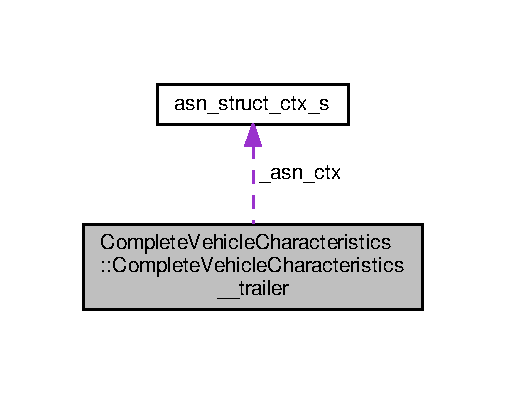
\includegraphics[width=243pt]{structCompleteVehicleCharacteristics_1_1CompleteVehicleCharacteristics____trailer__coll__graph}
\end{center}
\end{figure}
\subsection*{Public Member Functions}
\begin{DoxyCompactItemize}
\item 
{\bfseries A\+\_\+\+S\+E\+Q\+U\+E\+N\+C\+E\+\_\+\+OF} (struct \hyperlink{structTrailerCharacteristics}{Trailer\+Characteristics}) list\hypertarget{structCompleteVehicleCharacteristics_1_1CompleteVehicleCharacteristics____trailer_ae481841670599e0ce96287172adcbc0e}{}\label{structCompleteVehicleCharacteristics_1_1CompleteVehicleCharacteristics____trailer_ae481841670599e0ce96287172adcbc0e}

\end{DoxyCompactItemize}
\subsection*{Public Attributes}
\begin{DoxyCompactItemize}
\item 
\hyperlink{structasn__struct__ctx__s}{asn\+\_\+struct\+\_\+ctx\+\_\+t} {\bfseries \+\_\+asn\+\_\+ctx}\hypertarget{structCompleteVehicleCharacteristics_1_1CompleteVehicleCharacteristics____trailer_aeb666deec9754ab85b3947a9cd36c4ed}{}\label{structCompleteVehicleCharacteristics_1_1CompleteVehicleCharacteristics____trailer_aeb666deec9754ab85b3947a9cd36c4ed}

\end{DoxyCompactItemize}


The documentation for this struct was generated from the following file\+:\begin{DoxyCompactItemize}
\item 
include/aimsun\+\_\+extensions/\+V2\+X\+Framework/\+I\+T\+S-\/spec/Complete\+Vehicle\+Characteristics.\+h\end{DoxyCompactItemize}

\hypertarget{structComputedLane}{}\section{Computed\+Lane Struct Reference}
\label{structComputedLane}\index{Computed\+Lane@{Computed\+Lane}}


Collaboration diagram for Computed\+Lane\+:\nopagebreak
\begin{figure}[H]
\begin{center}
\leavevmode
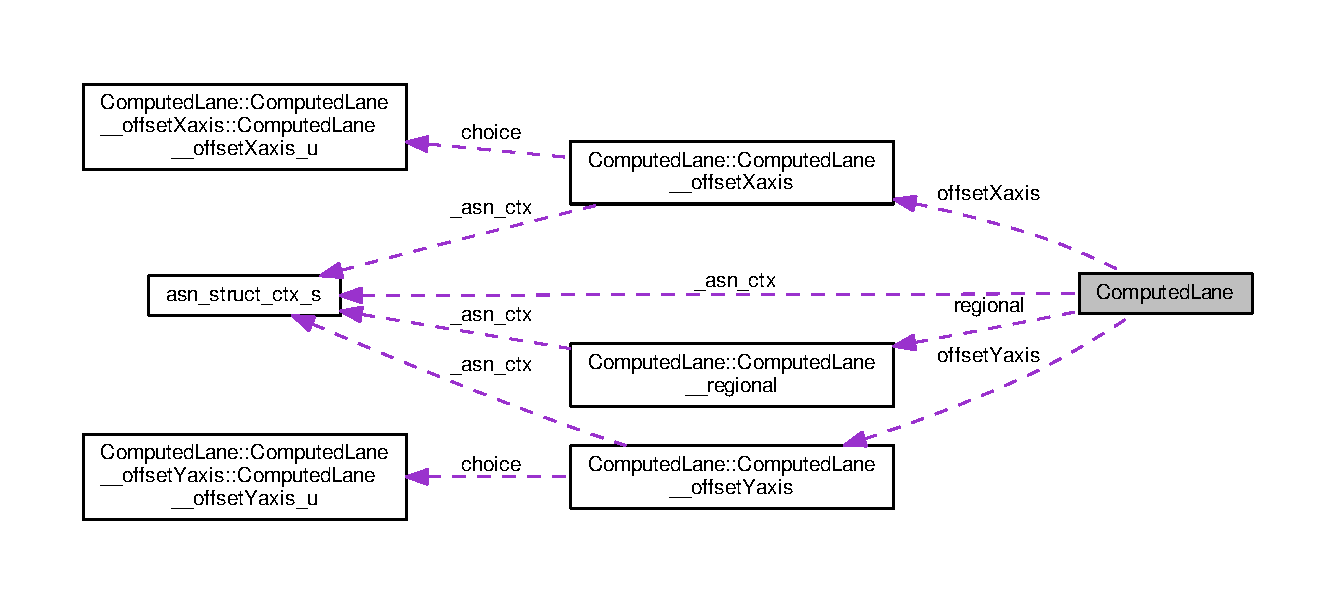
\includegraphics[width=350pt]{structComputedLane__coll__graph}
\end{center}
\end{figure}
\subsection*{Classes}
\begin{DoxyCompactItemize}
\item 
struct \hyperlink{structComputedLane_1_1ComputedLane____offsetXaxis}{Computed\+Lane\+\_\+\+\_\+offset\+Xaxis}
\item 
struct \hyperlink{structComputedLane_1_1ComputedLane____offsetYaxis}{Computed\+Lane\+\_\+\+\_\+offset\+Yaxis}
\item 
struct \hyperlink{structComputedLane_1_1ComputedLane____regional}{Computed\+Lane\+\_\+\+\_\+regional}
\end{DoxyCompactItemize}
\subsection*{Public Attributes}
\begin{DoxyCompactItemize}
\item 
Lane\+I\+D\+\_\+t {\bfseries reference\+Lane\+Id}\hypertarget{structComputedLane_a6bed2aeb9e11fdcacdcd30dbc1914c0b}{}\label{structComputedLane_a6bed2aeb9e11fdcacdcd30dbc1914c0b}

\item 
struct \hyperlink{structComputedLane_1_1ComputedLane____offsetXaxis}{Computed\+Lane\+::\+Computed\+Lane\+\_\+\+\_\+offset\+Xaxis} {\bfseries offset\+Xaxis}\hypertarget{structComputedLane_afc8ac4eed711e796ebb52ea10edf07f0}{}\label{structComputedLane_afc8ac4eed711e796ebb52ea10edf07f0}

\item 
struct \hyperlink{structComputedLane_1_1ComputedLane____offsetYaxis}{Computed\+Lane\+::\+Computed\+Lane\+\_\+\+\_\+offset\+Yaxis} {\bfseries offset\+Yaxis}\hypertarget{structComputedLane_a161a05a776c4e6470da7a4ae7d6766bc}{}\label{structComputedLane_a161a05a776c4e6470da7a4ae7d6766bc}

\item 
Angle\+\_\+t $\ast$ {\bfseries rotate\+XY}\hypertarget{structComputedLane_a49753e6dfcbf7a52079ddf3d513a3a97}{}\label{structComputedLane_a49753e6dfcbf7a52079ddf3d513a3a97}

\item 
Scale\+\_\+\+B12\+\_\+t $\ast$ {\bfseries scale\+Xaxis}\hypertarget{structComputedLane_a5744c32d0634e994faa43c176a7e4320}{}\label{structComputedLane_a5744c32d0634e994faa43c176a7e4320}

\item 
Scale\+\_\+\+B12\+\_\+t $\ast$ {\bfseries scale\+Yaxis}\hypertarget{structComputedLane_a5923c691d8c695f2eca4bb7b3bf5f8a2}{}\label{structComputedLane_a5923c691d8c695f2eca4bb7b3bf5f8a2}

\item 
struct \hyperlink{structComputedLane_1_1ComputedLane____regional}{Computed\+Lane\+::\+Computed\+Lane\+\_\+\+\_\+regional} $\ast$ {\bfseries regional}\hypertarget{structComputedLane_a76ea24d60623d4363cbfcb7b82b9de5e}{}\label{structComputedLane_a76ea24d60623d4363cbfcb7b82b9de5e}

\item 
\hyperlink{structasn__struct__ctx__s}{asn\+\_\+struct\+\_\+ctx\+\_\+t} {\bfseries \+\_\+asn\+\_\+ctx}\hypertarget{structComputedLane_a82776cb9fe58ce2d4f698b8f8fd4c3c3}{}\label{structComputedLane_a82776cb9fe58ce2d4f698b8f8fd4c3c3}

\end{DoxyCompactItemize}


The documentation for this struct was generated from the following file\+:\begin{DoxyCompactItemize}
\item 
include/aimsun\+\_\+extensions/\+V2\+X\+Framework/\+I\+T\+S-\/spec/Computed\+Lane.\+h\end{DoxyCompactItemize}

\hypertarget{structComputedLane_1_1ComputedLane____offsetXaxis}{}\section{Computed\+Lane\+:\+:Computed\+Lane\+\_\+\+\_\+offset\+Xaxis Struct Reference}
\label{structComputedLane_1_1ComputedLane____offsetXaxis}\index{Computed\+Lane\+::\+Computed\+Lane\+\_\+\+\_\+offset\+Xaxis@{Computed\+Lane\+::\+Computed\+Lane\+\_\+\+\_\+offset\+Xaxis}}


Collaboration diagram for Computed\+Lane\+:\+:Computed\+Lane\+\_\+\+\_\+offset\+Xaxis\+:\nopagebreak
\begin{figure}[H]
\begin{center}
\leavevmode
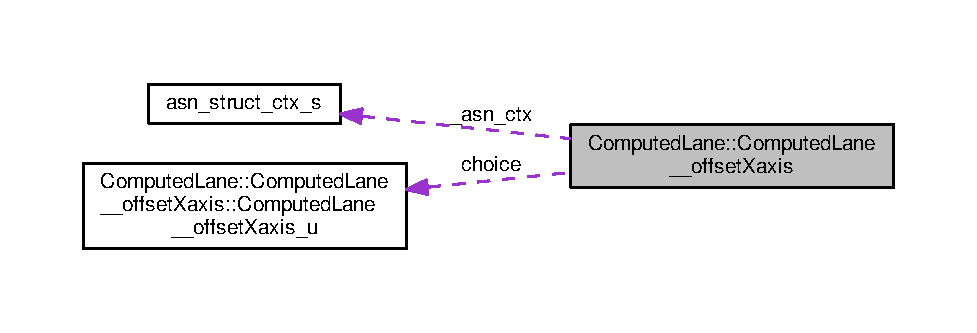
\includegraphics[width=350pt]{structComputedLane_1_1ComputedLane____offsetXaxis__coll__graph}
\end{center}
\end{figure}
\subsection*{Classes}
\begin{DoxyCompactItemize}
\item 
union \hyperlink{unionComputedLane_1_1ComputedLane____offsetXaxis_1_1ComputedLane____offsetXaxis__u}{Computed\+Lane\+\_\+\+\_\+offset\+Xaxis\+\_\+u}
\end{DoxyCompactItemize}
\subsection*{Public Attributes}
\begin{DoxyCompactItemize}
\item 
Computed\+Lane\+\_\+\+\_\+offset\+Xaxis\+\_\+\+PR {\bfseries present}\hypertarget{structComputedLane_1_1ComputedLane____offsetXaxis_aae3fe9ba4c706d959427af90ff889f87}{}\label{structComputedLane_1_1ComputedLane____offsetXaxis_aae3fe9ba4c706d959427af90ff889f87}

\item 
union \hyperlink{unionComputedLane_1_1ComputedLane____offsetXaxis_1_1ComputedLane____offsetXaxis__u}{Computed\+Lane\+::\+Computed\+Lane\+\_\+\+\_\+offset\+Xaxis\+::\+Computed\+Lane\+\_\+\+\_\+offset\+Xaxis\+\_\+u} {\bfseries choice}\hypertarget{structComputedLane_1_1ComputedLane____offsetXaxis_aec23a4d80994e557425bff3489c83122}{}\label{structComputedLane_1_1ComputedLane____offsetXaxis_aec23a4d80994e557425bff3489c83122}

\item 
\hyperlink{structasn__struct__ctx__s}{asn\+\_\+struct\+\_\+ctx\+\_\+t} {\bfseries \+\_\+asn\+\_\+ctx}\hypertarget{structComputedLane_1_1ComputedLane____offsetXaxis_adebebb248b7c19965d3d89992f525c2a}{}\label{structComputedLane_1_1ComputedLane____offsetXaxis_adebebb248b7c19965d3d89992f525c2a}

\end{DoxyCompactItemize}


The documentation for this struct was generated from the following file\+:\begin{DoxyCompactItemize}
\item 
include/aimsun\+\_\+extensions/\+V2\+X\+Framework/\+I\+T\+S-\/spec/Computed\+Lane.\+h\end{DoxyCompactItemize}

\hypertarget{unionComputedLane_1_1ComputedLane____offsetXaxis_1_1ComputedLane____offsetXaxis__u}{}\section{Computed\+Lane\+:\+:Computed\+Lane\+\_\+\+\_\+offset\+Xaxis\+:\+:Computed\+Lane\+\_\+\+\_\+offset\+Xaxis\+\_\+u Union Reference}
\label{unionComputedLane_1_1ComputedLane____offsetXaxis_1_1ComputedLane____offsetXaxis__u}\index{Computed\+Lane\+::\+Computed\+Lane\+\_\+\+\_\+offset\+Xaxis\+::\+Computed\+Lane\+\_\+\+\_\+offset\+Xaxis\+\_\+u@{Computed\+Lane\+::\+Computed\+Lane\+\_\+\+\_\+offset\+Xaxis\+::\+Computed\+Lane\+\_\+\+\_\+offset\+Xaxis\+\_\+u}}
\subsection*{Public Attributes}
\begin{DoxyCompactItemize}
\item 
Driven\+Line\+Offset\+Sm\+\_\+t {\bfseries small}\hypertarget{unionComputedLane_1_1ComputedLane____offsetXaxis_1_1ComputedLane____offsetXaxis__u_ac4a2a617bb794ce411f841759169c3eb}{}\label{unionComputedLane_1_1ComputedLane____offsetXaxis_1_1ComputedLane____offsetXaxis__u_ac4a2a617bb794ce411f841759169c3eb}

\item 
Driven\+Line\+Offset\+Lg\+\_\+t {\bfseries large}\hypertarget{unionComputedLane_1_1ComputedLane____offsetXaxis_1_1ComputedLane____offsetXaxis__u_af706a172f5815246ad8dcf37bc09e92f}{}\label{unionComputedLane_1_1ComputedLane____offsetXaxis_1_1ComputedLane____offsetXaxis__u_af706a172f5815246ad8dcf37bc09e92f}

\end{DoxyCompactItemize}


The documentation for this union was generated from the following file\+:\begin{DoxyCompactItemize}
\item 
include/aimsun\+\_\+extensions/\+V2\+X\+Framework/\+I\+T\+S-\/spec/Computed\+Lane.\+h\end{DoxyCompactItemize}

\hypertarget{structComputedLane_1_1ComputedLane____offsetYaxis}{}\section{Computed\+Lane\+:\+:Computed\+Lane\+\_\+\+\_\+offset\+Yaxis Struct Reference}
\label{structComputedLane_1_1ComputedLane____offsetYaxis}\index{Computed\+Lane\+::\+Computed\+Lane\+\_\+\+\_\+offset\+Yaxis@{Computed\+Lane\+::\+Computed\+Lane\+\_\+\+\_\+offset\+Yaxis}}


Collaboration diagram for Computed\+Lane\+:\+:Computed\+Lane\+\_\+\+\_\+offset\+Yaxis\+:\nopagebreak
\begin{figure}[H]
\begin{center}
\leavevmode
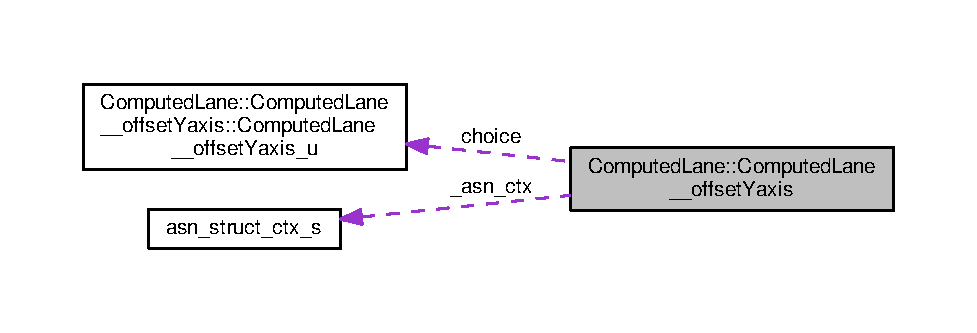
\includegraphics[width=350pt]{structComputedLane_1_1ComputedLane____offsetYaxis__coll__graph}
\end{center}
\end{figure}
\subsection*{Classes}
\begin{DoxyCompactItemize}
\item 
union \hyperlink{unionComputedLane_1_1ComputedLane____offsetYaxis_1_1ComputedLane____offsetYaxis__u}{Computed\+Lane\+\_\+\+\_\+offset\+Yaxis\+\_\+u}
\end{DoxyCompactItemize}
\subsection*{Public Attributes}
\begin{DoxyCompactItemize}
\item 
Computed\+Lane\+\_\+\+\_\+offset\+Yaxis\+\_\+\+PR {\bfseries present}\hypertarget{structComputedLane_1_1ComputedLane____offsetYaxis_a23c45f14fc0947c46ce80bfa06c99e42}{}\label{structComputedLane_1_1ComputedLane____offsetYaxis_a23c45f14fc0947c46ce80bfa06c99e42}

\item 
union \hyperlink{unionComputedLane_1_1ComputedLane____offsetYaxis_1_1ComputedLane____offsetYaxis__u}{Computed\+Lane\+::\+Computed\+Lane\+\_\+\+\_\+offset\+Yaxis\+::\+Computed\+Lane\+\_\+\+\_\+offset\+Yaxis\+\_\+u} {\bfseries choice}\hypertarget{structComputedLane_1_1ComputedLane____offsetYaxis_a045bf7c373361f52020225390809404c}{}\label{structComputedLane_1_1ComputedLane____offsetYaxis_a045bf7c373361f52020225390809404c}

\item 
\hyperlink{structasn__struct__ctx__s}{asn\+\_\+struct\+\_\+ctx\+\_\+t} {\bfseries \+\_\+asn\+\_\+ctx}\hypertarget{structComputedLane_1_1ComputedLane____offsetYaxis_a839809f017c8d6e5a0bf273e399a9bac}{}\label{structComputedLane_1_1ComputedLane____offsetYaxis_a839809f017c8d6e5a0bf273e399a9bac}

\end{DoxyCompactItemize}


The documentation for this struct was generated from the following file\+:\begin{DoxyCompactItemize}
\item 
include/aimsun\+\_\+extensions/\+V2\+X\+Framework/\+I\+T\+S-\/spec/Computed\+Lane.\+h\end{DoxyCompactItemize}

\hypertarget{unionComputedLane_1_1ComputedLane____offsetYaxis_1_1ComputedLane____offsetYaxis__u}{}\section{Computed\+Lane\+:\+:Computed\+Lane\+\_\+\+\_\+offset\+Yaxis\+:\+:Computed\+Lane\+\_\+\+\_\+offset\+Yaxis\+\_\+u Union Reference}
\label{unionComputedLane_1_1ComputedLane____offsetYaxis_1_1ComputedLane____offsetYaxis__u}\index{Computed\+Lane\+::\+Computed\+Lane\+\_\+\+\_\+offset\+Yaxis\+::\+Computed\+Lane\+\_\+\+\_\+offset\+Yaxis\+\_\+u@{Computed\+Lane\+::\+Computed\+Lane\+\_\+\+\_\+offset\+Yaxis\+::\+Computed\+Lane\+\_\+\+\_\+offset\+Yaxis\+\_\+u}}
\subsection*{Public Attributes}
\begin{DoxyCompactItemize}
\item 
Driven\+Line\+Offset\+Sm\+\_\+t {\bfseries small}\hypertarget{unionComputedLane_1_1ComputedLane____offsetYaxis_1_1ComputedLane____offsetYaxis__u_a2eeef670b102d41a864e646ef968605a}{}\label{unionComputedLane_1_1ComputedLane____offsetYaxis_1_1ComputedLane____offsetYaxis__u_a2eeef670b102d41a864e646ef968605a}

\item 
Driven\+Line\+Offset\+Lg\+\_\+t {\bfseries large}\hypertarget{unionComputedLane_1_1ComputedLane____offsetYaxis_1_1ComputedLane____offsetYaxis__u_a07f79d04ef527b8090632bcb8bea9792}{}\label{unionComputedLane_1_1ComputedLane____offsetYaxis_1_1ComputedLane____offsetYaxis__u_a07f79d04ef527b8090632bcb8bea9792}

\end{DoxyCompactItemize}


The documentation for this union was generated from the following file\+:\begin{DoxyCompactItemize}
\item 
include/aimsun\+\_\+extensions/\+V2\+X\+Framework/\+I\+T\+S-\/spec/Computed\+Lane.\+h\end{DoxyCompactItemize}

\hypertarget{structComputedLane_1_1ComputedLane____regional}{}\section{Computed\+Lane\+:\+:Computed\+Lane\+\_\+\+\_\+regional Struct Reference}
\label{structComputedLane_1_1ComputedLane____regional}\index{Computed\+Lane\+::\+Computed\+Lane\+\_\+\+\_\+regional@{Computed\+Lane\+::\+Computed\+Lane\+\_\+\+\_\+regional}}


Collaboration diagram for Computed\+Lane\+:\+:Computed\+Lane\+\_\+\+\_\+regional\+:\nopagebreak
\begin{figure}[H]
\begin{center}
\leavevmode
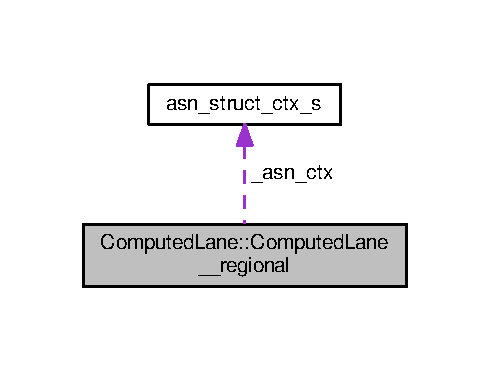
\includegraphics[width=235pt]{structComputedLane_1_1ComputedLane____regional__coll__graph}
\end{center}
\end{figure}
\subsection*{Public Member Functions}
\begin{DoxyCompactItemize}
\item 
{\bfseries A\+\_\+\+S\+E\+Q\+U\+E\+N\+C\+E\+\_\+\+OF} (struct Regional\+Extension) list\hypertarget{structComputedLane_1_1ComputedLane____regional_adeb8139c37e4651b95e777d74e23403d}{}\label{structComputedLane_1_1ComputedLane____regional_adeb8139c37e4651b95e777d74e23403d}

\end{DoxyCompactItemize}
\subsection*{Public Attributes}
\begin{DoxyCompactItemize}
\item 
\hyperlink{structasn__struct__ctx__s}{asn\+\_\+struct\+\_\+ctx\+\_\+t} {\bfseries \+\_\+asn\+\_\+ctx}\hypertarget{structComputedLane_1_1ComputedLane____regional_a6daf9c086abe33a6fe48fc6138b26852}{}\label{structComputedLane_1_1ComputedLane____regional_a6daf9c086abe33a6fe48fc6138b26852}

\end{DoxyCompactItemize}


The documentation for this struct was generated from the following file\+:\begin{DoxyCompactItemize}
\item 
include/aimsun\+\_\+extensions/\+V2\+X\+Framework/\+I\+T\+S-\/spec/Computed\+Lane.\+h\end{DoxyCompactItemize}

\hypertarget{structComputedSegment}{}\section{Computed\+Segment Struct Reference}
\label{structComputedSegment}\index{Computed\+Segment@{Computed\+Segment}}


Collaboration diagram for Computed\+Segment\+:\nopagebreak
\begin{figure}[H]
\begin{center}
\leavevmode
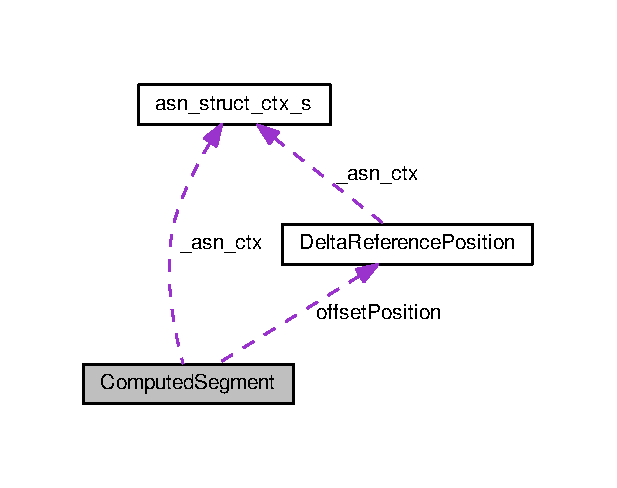
\includegraphics[width=296pt]{structComputedSegment__coll__graph}
\end{center}
\end{figure}
\subsection*{Public Attributes}
\begin{DoxyCompactItemize}
\item 
Zid\+\_\+t {\bfseries zone\+Id}\hypertarget{structComputedSegment_a4740feb45a20e11085c45ae27588b61a}{}\label{structComputedSegment_a4740feb45a20e11085c45ae27588b61a}

\item 
Lane\+Position\+\_\+t {\bfseries lane\+Number}\hypertarget{structComputedSegment_a00ded335eea383e6a1d9118d984a1464}{}\label{structComputedSegment_a00ded335eea383e6a1d9118d984a1464}

\item 
I\+V\+I\+Lane\+Width\+\_\+t {\bfseries lane\+Width}\hypertarget{structComputedSegment_a987998a435163b01cfdf8a4dd7a7bec4}{}\label{structComputedSegment_a987998a435163b01cfdf8a4dd7a7bec4}

\item 
long $\ast$ {\bfseries offset\+Distance}\hypertarget{structComputedSegment_af09f6a29e1f74f89f0c9a36b2f50df01}{}\label{structComputedSegment_af09f6a29e1f74f89f0c9a36b2f50df01}

\item 
struct \hyperlink{structDeltaReferencePosition}{Delta\+Reference\+Position} $\ast$ {\bfseries offset\+Position}\hypertarget{structComputedSegment_a1f1dfd0ba0ee3edece67a09a4b634bd0}{}\label{structComputedSegment_a1f1dfd0ba0ee3edece67a09a4b634bd0}

\item 
\hyperlink{structasn__struct__ctx__s}{asn\+\_\+struct\+\_\+ctx\+\_\+t} {\bfseries \+\_\+asn\+\_\+ctx}\hypertarget{structComputedSegment_acb3b847de0c71b06ec0146efaaa2d5af}{}\label{structComputedSegment_acb3b847de0c71b06ec0146efaaa2d5af}

\end{DoxyCompactItemize}


The documentation for this struct was generated from the following file\+:\begin{DoxyCompactItemize}
\item 
include/aimsun\+\_\+extensions/\+V2\+X\+Framework/\+I\+T\+S-\/spec/Computed\+Segment.\+h\end{DoxyCompactItemize}

\hypertarget{structConnectingLane}{}\section{Connecting\+Lane Struct Reference}
\label{structConnectingLane}\index{Connecting\+Lane@{Connecting\+Lane}}


Collaboration diagram for Connecting\+Lane\+:\nopagebreak
\begin{figure}[H]
\begin{center}
\leavevmode
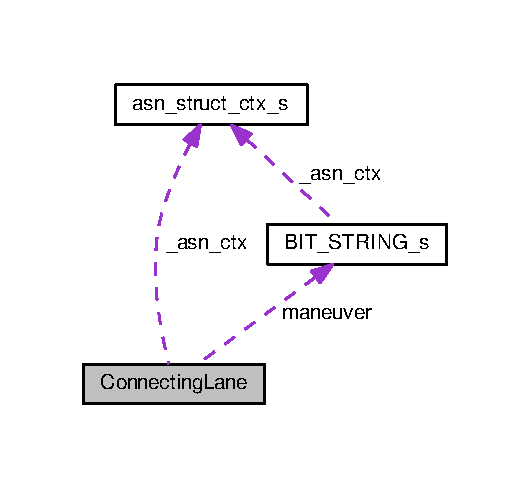
\includegraphics[width=255pt]{structConnectingLane__coll__graph}
\end{center}
\end{figure}
\subsection*{Public Attributes}
\begin{DoxyCompactItemize}
\item 
Lane\+I\+D\+\_\+t {\bfseries lane}\hypertarget{structConnectingLane_a28a86da9e6e5486db16650936e631859}{}\label{structConnectingLane_a28a86da9e6e5486db16650936e631859}

\item 
\hyperlink{structBIT__STRING__s}{Allowed\+Maneuvers\+\_\+t} $\ast$ {\bfseries maneuver}\hypertarget{structConnectingLane_a51be547597e5d84dfa829dcfd4c94adb}{}\label{structConnectingLane_a51be547597e5d84dfa829dcfd4c94adb}

\item 
\hyperlink{structasn__struct__ctx__s}{asn\+\_\+struct\+\_\+ctx\+\_\+t} {\bfseries \+\_\+asn\+\_\+ctx}\hypertarget{structConnectingLane_aa01b73a021a88127fd0e7fc0d2efce07}{}\label{structConnectingLane_aa01b73a021a88127fd0e7fc0d2efce07}

\end{DoxyCompactItemize}


The documentation for this struct was generated from the following file\+:\begin{DoxyCompactItemize}
\item 
include/aimsun\+\_\+extensions/\+V2\+X\+Framework/\+I\+T\+S-\/spec/Connecting\+Lane.\+h\end{DoxyCompactItemize}

\hypertarget{structConnection}{}\section{Connection Struct Reference}
\label{structConnection}\index{Connection@{Connection}}


Collaboration diagram for Connection\+:\nopagebreak
\begin{figure}[H]
\begin{center}
\leavevmode
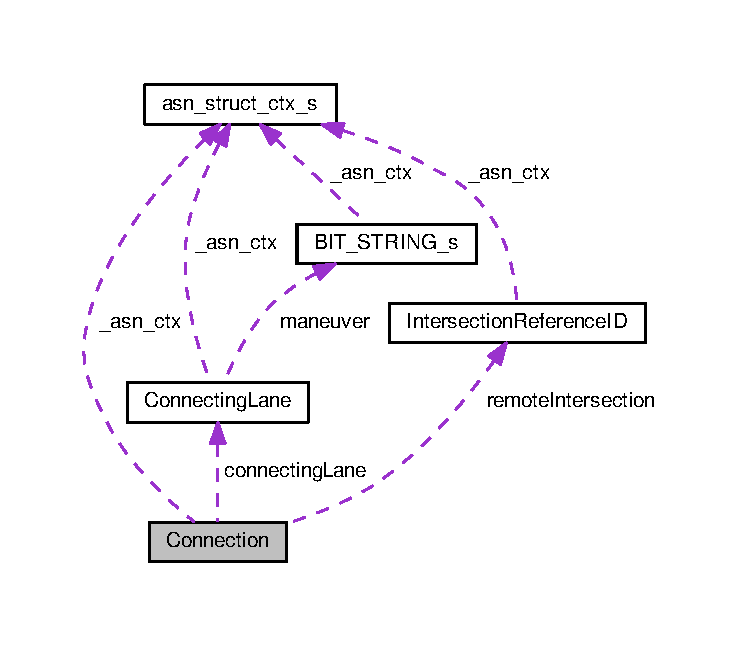
\includegraphics[width=350pt]{structConnection__coll__graph}
\end{center}
\end{figure}
\subsection*{Public Attributes}
\begin{DoxyCompactItemize}
\item 
\hyperlink{structConnectingLane}{Connecting\+Lane\+\_\+t} {\bfseries connecting\+Lane}\hypertarget{structConnection_abf7076c7b6cd26ba4e87ef6023451885}{}\label{structConnection_abf7076c7b6cd26ba4e87ef6023451885}

\item 
struct \hyperlink{structIntersectionReferenceID}{Intersection\+Reference\+ID} $\ast$ {\bfseries remote\+Intersection}\hypertarget{structConnection_a698019bf92265a99ab4a3b78237798a7}{}\label{structConnection_a698019bf92265a99ab4a3b78237798a7}

\item 
Signal\+Group\+I\+D\+\_\+t $\ast$ {\bfseries signal\+Group}\hypertarget{structConnection_a625bac5138cc65604c5b66f07b80385e}{}\label{structConnection_a625bac5138cc65604c5b66f07b80385e}

\item 
Restriction\+Class\+I\+D\+\_\+t $\ast$ {\bfseries user\+Class}\hypertarget{structConnection_ad404bb5ce45fe0c4e93466be6aae2fd0}{}\label{structConnection_ad404bb5ce45fe0c4e93466be6aae2fd0}

\item 
Lane\+Connection\+I\+D\+\_\+t $\ast$ {\bfseries connection\+ID}\hypertarget{structConnection_afcf4e4c5705173fa0464c7b26f508bcb}{}\label{structConnection_afcf4e4c5705173fa0464c7b26f508bcb}

\item 
\hyperlink{structasn__struct__ctx__s}{asn\+\_\+struct\+\_\+ctx\+\_\+t} {\bfseries \+\_\+asn\+\_\+ctx}\hypertarget{structConnection_a5f9a444f919809759dfb089929b310ee}{}\label{structConnection_a5f9a444f919809759dfb089929b310ee}

\end{DoxyCompactItemize}


The documentation for this struct was generated from the following file\+:\begin{DoxyCompactItemize}
\item 
include/aimsun\+\_\+extensions/\+V2\+X\+Framework/\+I\+T\+S-\/spec/Connection.\+h\end{DoxyCompactItemize}

\hypertarget{structConnectionManeuverAssist}{}\section{Connection\+Maneuver\+Assist Struct Reference}
\label{structConnectionManeuverAssist}\index{Connection\+Maneuver\+Assist@{Connection\+Maneuver\+Assist}}


Collaboration diagram for Connection\+Maneuver\+Assist\+:\nopagebreak
\begin{figure}[H]
\begin{center}
\leavevmode
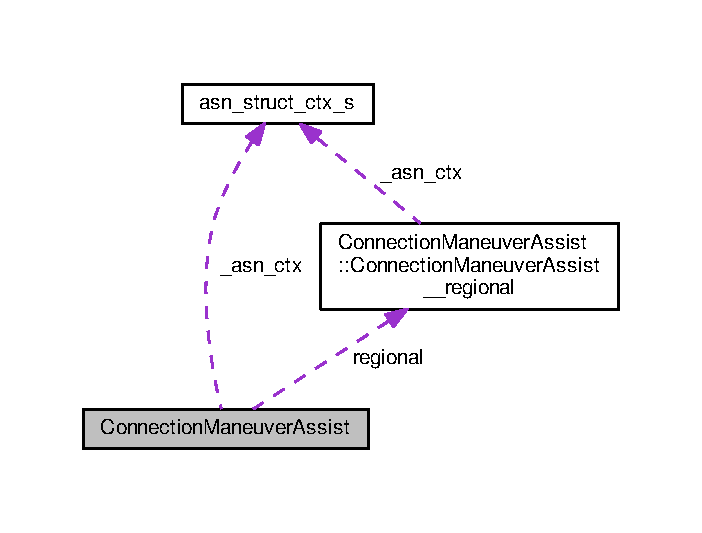
\includegraphics[width=337pt]{structConnectionManeuverAssist__coll__graph}
\end{center}
\end{figure}
\subsection*{Classes}
\begin{DoxyCompactItemize}
\item 
struct \hyperlink{structConnectionManeuverAssist_1_1ConnectionManeuverAssist____regional}{Connection\+Maneuver\+Assist\+\_\+\+\_\+regional}
\end{DoxyCompactItemize}
\subsection*{Public Attributes}
\begin{DoxyCompactItemize}
\item 
Lane\+Connection\+I\+D\+\_\+t {\bfseries connection\+ID}\hypertarget{structConnectionManeuverAssist_afac8b991af39c0942452aeea2865faa1}{}\label{structConnectionManeuverAssist_afac8b991af39c0942452aeea2865faa1}

\item 
Zone\+Length\+\_\+t $\ast$ {\bfseries queue\+Length}\hypertarget{structConnectionManeuverAssist_a89ffe08c65eaffcc7bbc580acb9708ee}{}\label{structConnectionManeuverAssist_a89ffe08c65eaffcc7bbc580acb9708ee}

\item 
Zone\+Length\+\_\+t $\ast$ {\bfseries available\+Storage\+Length}\hypertarget{structConnectionManeuverAssist_abc6b3d69f6242b184f18de0367a2ea7e}{}\label{structConnectionManeuverAssist_abc6b3d69f6242b184f18de0367a2ea7e}

\item 
Wait\+On\+Stopline\+\_\+t $\ast$ {\bfseries wait\+On\+Stop}\hypertarget{structConnectionManeuverAssist_a7bd74b6f26851952a6abb579311fc274}{}\label{structConnectionManeuverAssist_a7bd74b6f26851952a6abb579311fc274}

\item 
Pedestrian\+Bicycle\+Detect\+\_\+t $\ast$ {\bfseries ped\+Bicycle\+Detect}\hypertarget{structConnectionManeuverAssist_a1ea595de6a5845a1853d4c4817936deb}{}\label{structConnectionManeuverAssist_a1ea595de6a5845a1853d4c4817936deb}

\item 
struct \hyperlink{structConnectionManeuverAssist_1_1ConnectionManeuverAssist____regional}{Connection\+Maneuver\+Assist\+::\+Connection\+Maneuver\+Assist\+\_\+\+\_\+regional} $\ast$ {\bfseries regional}\hypertarget{structConnectionManeuverAssist_a26ec30919c70ad0988976ed49d962b2f}{}\label{structConnectionManeuverAssist_a26ec30919c70ad0988976ed49d962b2f}

\item 
\hyperlink{structasn__struct__ctx__s}{asn\+\_\+struct\+\_\+ctx\+\_\+t} {\bfseries \+\_\+asn\+\_\+ctx}\hypertarget{structConnectionManeuverAssist_a26f74a7a4c5c80fc2bccba95457c40af}{}\label{structConnectionManeuverAssist_a26f74a7a4c5c80fc2bccba95457c40af}

\end{DoxyCompactItemize}


The documentation for this struct was generated from the following file\+:\begin{DoxyCompactItemize}
\item 
include/aimsun\+\_\+extensions/\+V2\+X\+Framework/\+I\+T\+S-\/spec/Connection\+Maneuver\+Assist.\+h\end{DoxyCompactItemize}

\hypertarget{structConnectionManeuverAssist_1_1ConnectionManeuverAssist____regional}{}\section{Connection\+Maneuver\+Assist\+:\+:Connection\+Maneuver\+Assist\+\_\+\+\_\+regional Struct Reference}
\label{structConnectionManeuverAssist_1_1ConnectionManeuverAssist____regional}\index{Connection\+Maneuver\+Assist\+::\+Connection\+Maneuver\+Assist\+\_\+\+\_\+regional@{Connection\+Maneuver\+Assist\+::\+Connection\+Maneuver\+Assist\+\_\+\+\_\+regional}}


Collaboration diagram for Connection\+Maneuver\+Assist\+:\+:Connection\+Maneuver\+Assist\+\_\+\+\_\+regional\+:\nopagebreak
\begin{figure}[H]
\begin{center}
\leavevmode
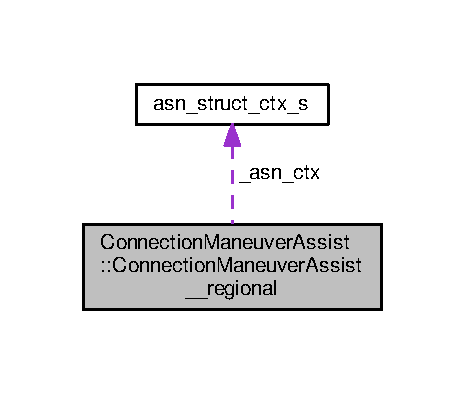
\includegraphics[width=223pt]{structConnectionManeuverAssist_1_1ConnectionManeuverAssist____regional__coll__graph}
\end{center}
\end{figure}
\subsection*{Public Member Functions}
\begin{DoxyCompactItemize}
\item 
{\bfseries A\+\_\+\+S\+E\+Q\+U\+E\+N\+C\+E\+\_\+\+OF} (struct Regional\+Extension) list\hypertarget{structConnectionManeuverAssist_1_1ConnectionManeuverAssist____regional_a3c83dad83b808f55f20fe3b6f4047d75}{}\label{structConnectionManeuverAssist_1_1ConnectionManeuverAssist____regional_a3c83dad83b808f55f20fe3b6f4047d75}

\end{DoxyCompactItemize}
\subsection*{Public Attributes}
\begin{DoxyCompactItemize}
\item 
\hyperlink{structasn__struct__ctx__s}{asn\+\_\+struct\+\_\+ctx\+\_\+t} {\bfseries \+\_\+asn\+\_\+ctx}\hypertarget{structConnectionManeuverAssist_1_1ConnectionManeuverAssist____regional_a43bb2198b1649ce2f63cd8f3ea636335}{}\label{structConnectionManeuverAssist_1_1ConnectionManeuverAssist____regional_a43bb2198b1649ce2f63cd8f3ea636335}

\end{DoxyCompactItemize}


The documentation for this struct was generated from the following file\+:\begin{DoxyCompactItemize}
\item 
include/aimsun\+\_\+extensions/\+V2\+X\+Framework/\+I\+T\+S-\/spec/Connection\+Maneuver\+Assist.\+h\end{DoxyCompactItemize}

\hypertarget{structConnectionManeuverAssist__addGrpC}{}\section{Connection\+Maneuver\+Assist\+\_\+add\+GrpC Struct Reference}
\label{structConnectionManeuverAssist__addGrpC}\index{Connection\+Maneuver\+Assist\+\_\+add\+GrpC@{Connection\+Maneuver\+Assist\+\_\+add\+GrpC}}


Collaboration diagram for Connection\+Maneuver\+Assist\+\_\+add\+GrpC\+:\nopagebreak
\begin{figure}[H]
\begin{center}
\leavevmode
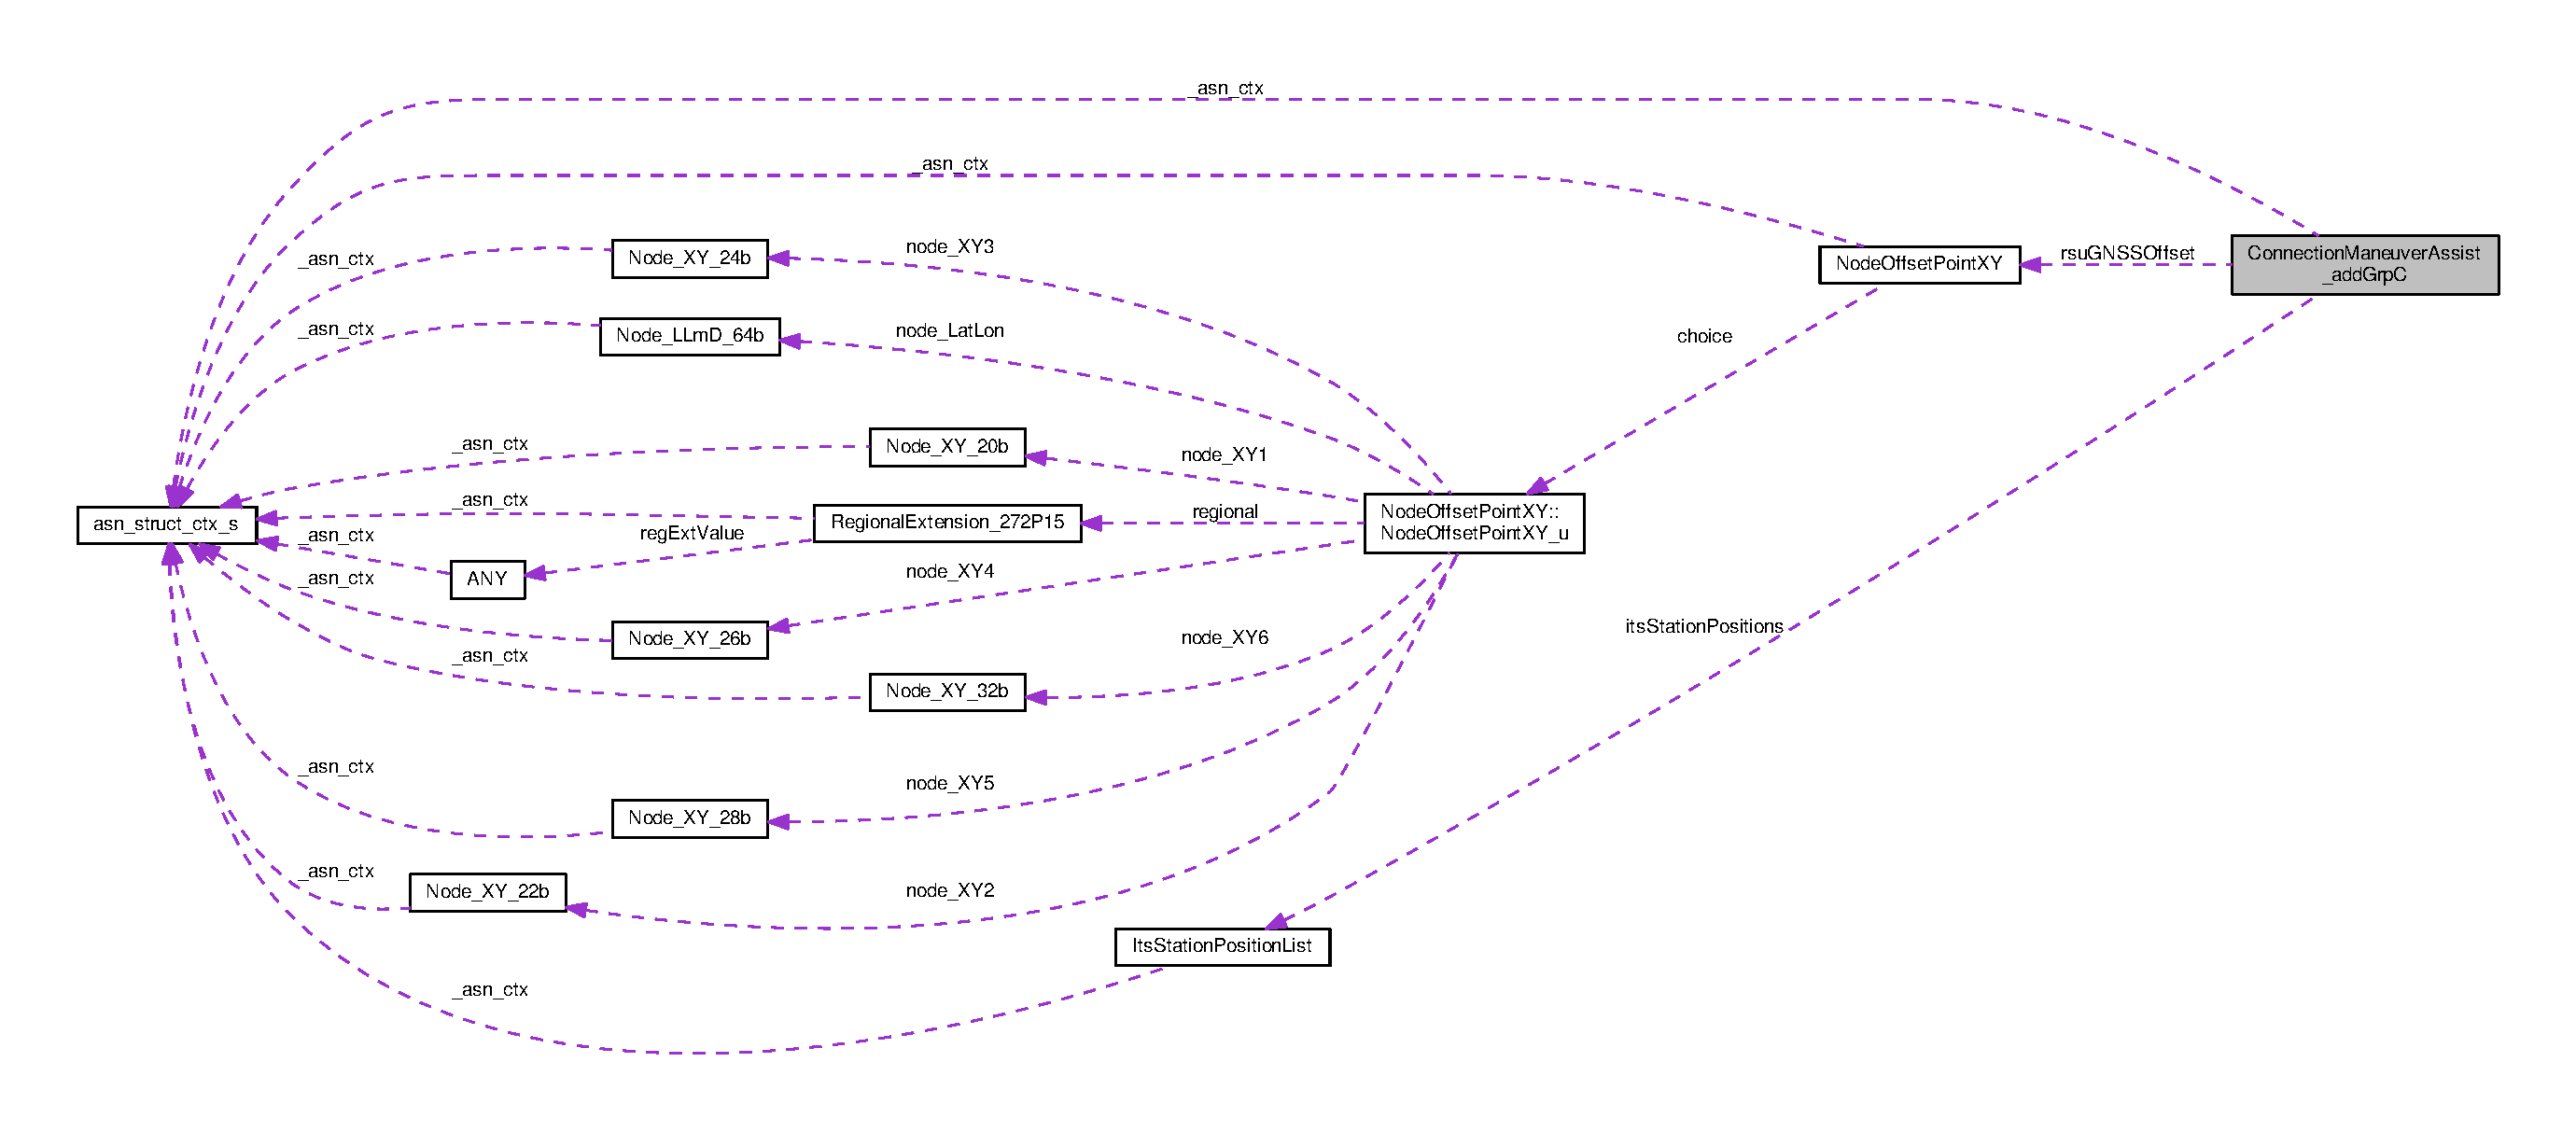
\includegraphics[width=350pt]{structConnectionManeuverAssist__addGrpC__coll__graph}
\end{center}
\end{figure}
\subsection*{Public Attributes}
\begin{DoxyCompactItemize}
\item 
struct \hyperlink{structItsStationPositionList}{Its\+Station\+Position\+List} $\ast$ {\bfseries its\+Station\+Positions}\hypertarget{structConnectionManeuverAssist__addGrpC_a27ff06cb85fad47712cc8053eb151d5e}{}\label{structConnectionManeuverAssist__addGrpC_a27ff06cb85fad47712cc8053eb151d5e}

\item 
struct \hyperlink{structNodeOffsetPointXY}{Node\+Offset\+Point\+XY} $\ast$ {\bfseries rsu\+G\+N\+S\+S\+Offset}\hypertarget{structConnectionManeuverAssist__addGrpC_a1b8cba23916d0528c2905401614126b0}{}\label{structConnectionManeuverAssist__addGrpC_a1b8cba23916d0528c2905401614126b0}

\item 
\hyperlink{structasn__struct__ctx__s}{asn\+\_\+struct\+\_\+ctx\+\_\+t} {\bfseries \+\_\+asn\+\_\+ctx}\hypertarget{structConnectionManeuverAssist__addGrpC_ae62418896df028c71e4658d1def24e87}{}\label{structConnectionManeuverAssist__addGrpC_ae62418896df028c71e4658d1def24e87}

\end{DoxyCompactItemize}


The documentation for this struct was generated from the following file\+:\begin{DoxyCompactItemize}
\item 
include/aimsun\+\_\+extensions/\+V2\+X\+Framework/\+I\+T\+S-\/spec/Connection\+Maneuver\+Assist-\/add\+Grp\+C.\+h\end{DoxyCompactItemize}

\hypertarget{structConnectionTrajectory__addGrpC}{}\section{Connection\+Trajectory\+\_\+add\+GrpC Struct Reference}
\label{structConnectionTrajectory__addGrpC}\index{Connection\+Trajectory\+\_\+add\+GrpC@{Connection\+Trajectory\+\_\+add\+GrpC}}


Collaboration diagram for Connection\+Trajectory\+\_\+add\+GrpC\+:\nopagebreak
\begin{figure}[H]
\begin{center}
\leavevmode
\includegraphics[width=248pt]{structConnectionTrajectory__addGrpC__coll__graph}
\end{center}
\end{figure}
\subsection*{Public Attributes}
\begin{DoxyCompactItemize}
\item 
\hyperlink{structNodeSetXY}{Node\+Set\+X\+Y\+\_\+t} {\bfseries nodes}\hypertarget{structConnectionTrajectory__addGrpC_a49fda3ad4b77eb87faab77a9be25fc3b}{}\label{structConnectionTrajectory__addGrpC_a49fda3ad4b77eb87faab77a9be25fc3b}

\item 
\hyperlink{structasn__struct__ctx__s}{asn\+\_\+struct\+\_\+ctx\+\_\+t} {\bfseries \+\_\+asn\+\_\+ctx}\hypertarget{structConnectionTrajectory__addGrpC_a08e881b81b80c97221f4301f34347ca6}{}\label{structConnectionTrajectory__addGrpC_a08e881b81b80c97221f4301f34347ca6}

\end{DoxyCompactItemize}


The documentation for this struct was generated from the following file\+:\begin{DoxyCompactItemize}
\item 
include/aimsun\+\_\+extensions/\+V2\+X\+Framework/\+I\+T\+S-\/spec/Connection\+Trajectory-\/add\+Grp\+C.\+h\end{DoxyCompactItemize}

\hypertarget{structConnectsToList}{}\section{Connects\+To\+List Struct Reference}
\label{structConnectsToList}\index{Connects\+To\+List@{Connects\+To\+List}}


Collaboration diagram for Connects\+To\+List\+:\nopagebreak
\begin{figure}[H]
\begin{center}
\leavevmode
\includegraphics[width=172pt]{structConnectsToList__coll__graph}
\end{center}
\end{figure}
\subsection*{Public Member Functions}
\begin{DoxyCompactItemize}
\item 
{\bfseries A\+\_\+\+S\+E\+Q\+U\+E\+N\+C\+E\+\_\+\+OF} (struct \hyperlink{structConnection}{Connection}) list\hypertarget{structConnectsToList_a0b196d741902436143c7428584b9b15e}{}\label{structConnectsToList_a0b196d741902436143c7428584b9b15e}

\end{DoxyCompactItemize}
\subsection*{Public Attributes}
\begin{DoxyCompactItemize}
\item 
\hyperlink{structasn__struct__ctx__s}{asn\+\_\+struct\+\_\+ctx\+\_\+t} {\bfseries \+\_\+asn\+\_\+ctx}\hypertarget{structConnectsToList_afa1418992848f8bb3ad8ce21197e9a23}{}\label{structConnectsToList_afa1418992848f8bb3ad8ce21197e9a23}

\end{DoxyCompactItemize}


The documentation for this struct was generated from the following file\+:\begin{DoxyCompactItemize}
\item 
include/aimsun\+\_\+extensions/\+V2\+X\+Framework/\+I\+T\+S-\/spec/Connects\+To\+List.\+h\end{DoxyCompactItemize}

\hypertarget{structControl__addGrpC}{}\section{Control\+\_\+add\+GrpC Struct Reference}
\label{structControl__addGrpC}\index{Control\+\_\+add\+GrpC@{Control\+\_\+add\+GrpC}}


Collaboration diagram for Control\+\_\+add\+GrpC\+:\nopagebreak
\begin{figure}[H]
\begin{center}
\leavevmode
\includegraphics[width=172pt]{structControl__addGrpC__coll__graph}
\end{center}
\end{figure}
\subsection*{Public Attributes}
\begin{DoxyCompactItemize}
\item 
Ptv\+Request\+Type\+\_\+t {\bfseries ptv\+Request}\hypertarget{structControl__addGrpC_a2e765e6111fd901961cd031a6fd65562}{}\label{structControl__addGrpC_a2e765e6111fd901961cd031a6fd65562}

\item 
\hyperlink{structasn__struct__ctx__s}{asn\+\_\+struct\+\_\+ctx\+\_\+t} {\bfseries \+\_\+asn\+\_\+ctx}\hypertarget{structControl__addGrpC_aa30c6ae98bac08ac040cd6ec1772a2e8}{}\label{structControl__addGrpC_aa30c6ae98bac08ac040cd6ec1772a2e8}

\end{DoxyCompactItemize}


The documentation for this struct was generated from the following file\+:\begin{DoxyCompactItemize}
\item 
include/aimsun\+\_\+extensions/\+V2\+X\+Framework/\+I\+T\+S-\/spec/Control-\/add\+Grp\+C.\+h\end{DoxyCompactItemize}

\hypertarget{structCoopAwareness}{}\section{Coop\+Awareness Struct Reference}
\label{structCoopAwareness}\index{Coop\+Awareness@{Coop\+Awareness}}


Collaboration diagram for Coop\+Awareness\+:\nopagebreak
\begin{figure}[H]
\begin{center}
\leavevmode
\includegraphics[width=350pt]{structCoopAwareness__coll__graph}
\end{center}
\end{figure}
\subsection*{Public Attributes}
\begin{DoxyCompactItemize}
\item 
Generation\+Delta\+Time\+\_\+t {\bfseries generation\+Delta\+Time}\hypertarget{structCoopAwareness_a8eb3666de67fb36a5aa49ec807d682a3}{}\label{structCoopAwareness_a8eb3666de67fb36a5aa49ec807d682a3}

\item 
\hyperlink{structCamParameters}{Cam\+Parameters\+\_\+t} {\bfseries cam\+Parameters}\hypertarget{structCoopAwareness_a969dd0582ebd23fa02ec31771d39a396}{}\label{structCoopAwareness_a969dd0582ebd23fa02ec31771d39a396}

\item 
\hyperlink{structasn__struct__ctx__s}{asn\+\_\+struct\+\_\+ctx\+\_\+t} {\bfseries \+\_\+asn\+\_\+ctx}\hypertarget{structCoopAwareness_a2495ccf3cd1ce9d69938516588665e3c}{}\label{structCoopAwareness_a2495ccf3cd1ce9d69938516588665e3c}

\end{DoxyCompactItemize}


The documentation for this struct was generated from the following file\+:\begin{DoxyCompactItemize}
\item 
include/aimsun\+\_\+extensions/\+V2\+X\+Framework/\+I\+T\+S-\/spec/Coop\+Awareness.\+h\end{DoxyCompactItemize}

\hypertarget{structCS5}{}\section{C\+S5 Struct Reference}
\label{structCS5}\index{C\+S5@{C\+S5}}


Collaboration diagram for C\+S5\+:\nopagebreak
\begin{figure}[H]
\begin{center}
\leavevmode
\includegraphics[width=334pt]{structCS5__coll__graph}
\end{center}
\end{figure}
\subsection*{Public Attributes}
\begin{DoxyCompactItemize}
\item 
\hyperlink{structOCTET__STRING}{Visible\+String\+\_\+t} {\bfseries vin}\hypertarget{structCS5_a2754f094b3be072340386e12dbd5ad71}{}\label{structCS5_a2754f094b3be072340386e12dbd5ad71}

\item 
\hyperlink{structBIT__STRING__s}{B\+I\+T\+\_\+\+S\+T\+R\+I\+N\+G\+\_\+t} {\bfseries fill}\hypertarget{structCS5_ab6444c19b458277c296e216ffbad65ca}{}\label{structCS5_ab6444c19b458277c296e216ffbad65ca}

\item 
\hyperlink{structasn__struct__ctx__s}{asn\+\_\+struct\+\_\+ctx\+\_\+t} {\bfseries \+\_\+asn\+\_\+ctx}\hypertarget{structCS5_a21e9400c3f19a85eb8882eda1481b897}{}\label{structCS5_a21e9400c3f19a85eb8882eda1481b897}

\end{DoxyCompactItemize}


The documentation for this struct was generated from the following file\+:\begin{DoxyCompactItemize}
\item 
include/aimsun\+\_\+extensions/\+V2\+X\+Framework/\+I\+T\+S-\/spec/C\+S5.\+h\end{DoxyCompactItemize}

\hypertarget{structCurvature}{}\section{Curvature Struct Reference}
\label{structCurvature}\index{Curvature@{Curvature}}


Collaboration diagram for Curvature\+:\nopagebreak
\begin{figure}[H]
\begin{center}
\leavevmode
\includegraphics[width=172pt]{structCurvature__coll__graph}
\end{center}
\end{figure}
\subsection*{Public Attributes}
\begin{DoxyCompactItemize}
\item 
Curvature\+Value\+\_\+t {\bfseries curvature\+Value}\hypertarget{structCurvature_a95f6c13d4499eb9dd409df6507dde547}{}\label{structCurvature_a95f6c13d4499eb9dd409df6507dde547}

\item 
Curvature\+Confidence\+\_\+t {\bfseries curvature\+Confidence}\hypertarget{structCurvature_a21e297cd1422c9ecdf23c28493c0ad6a}{}\label{structCurvature_a21e297cd1422c9ecdf23c28493c0ad6a}

\item 
\hyperlink{structasn__struct__ctx__s}{asn\+\_\+struct\+\_\+ctx\+\_\+t} {\bfseries \+\_\+asn\+\_\+ctx}\hypertarget{structCurvature_aff39179be86af9e7286324f025fe1484}{}\label{structCurvature_aff39179be86af9e7286324f025fe1484}

\end{DoxyCompactItemize}


The documentation for this struct was generated from the following file\+:\begin{DoxyCompactItemize}
\item 
include/aimsun\+\_\+extensions/\+V2\+X\+Framework/\+I\+T\+S-\/spec/Curvature.\+h\end{DoxyCompactItemize}

\hypertarget{structDangerousGoodsContainer}{}\section{Dangerous\+Goods\+Container Struct Reference}
\label{structDangerousGoodsContainer}\index{Dangerous\+Goods\+Container@{Dangerous\+Goods\+Container}}


Collaboration diagram for Dangerous\+Goods\+Container\+:\nopagebreak
\begin{figure}[H]
\begin{center}
\leavevmode
\includegraphics[width=214pt]{structDangerousGoodsContainer__coll__graph}
\end{center}
\end{figure}
\subsection*{Public Attributes}
\begin{DoxyCompactItemize}
\item 
Dangerous\+Goods\+Basic\+\_\+t {\bfseries dangerous\+Goods\+Basic}\hypertarget{structDangerousGoodsContainer_a36720e3457b36cfae8bcdae92c24d052}{}\label{structDangerousGoodsContainer_a36720e3457b36cfae8bcdae92c24d052}

\item 
\hyperlink{structasn__struct__ctx__s}{asn\+\_\+struct\+\_\+ctx\+\_\+t} {\bfseries \+\_\+asn\+\_\+ctx}\hypertarget{structDangerousGoodsContainer_ad259bfb360ac97a0450809e830347204}{}\label{structDangerousGoodsContainer_ad259bfb360ac97a0450809e830347204}

\end{DoxyCompactItemize}


The documentation for this struct was generated from the following file\+:\begin{DoxyCompactItemize}
\item 
include/aimsun\+\_\+extensions/\+V2\+X\+Framework/\+I\+T\+S-\/spec/Dangerous\+Goods\+Container.\+h\end{DoxyCompactItemize}

\hypertarget{structDangerousGoodsExtended}{}\section{Dangerous\+Goods\+Extended Struct Reference}
\label{structDangerousGoodsExtended}\index{Dangerous\+Goods\+Extended@{Dangerous\+Goods\+Extended}}


Collaboration diagram for Dangerous\+Goods\+Extended\+:\nopagebreak
\begin{figure}[H]
\begin{center}
\leavevmode
\includegraphics[width=296pt]{structDangerousGoodsExtended__coll__graph}
\end{center}
\end{figure}
\subsection*{Public Attributes}
\begin{DoxyCompactItemize}
\item 
Dangerous\+Goods\+Basic\+\_\+t {\bfseries dangerous\+Goods\+Type}\hypertarget{structDangerousGoodsExtended_a31b018833d98444df5c248e44b992e86}{}\label{structDangerousGoodsExtended_a31b018833d98444df5c248e44b992e86}

\item 
long {\bfseries un\+Number}\hypertarget{structDangerousGoodsExtended_a925dea7ea368a0ab7a93c17d08c4992e}{}\label{structDangerousGoodsExtended_a925dea7ea368a0ab7a93c17d08c4992e}

\item 
B\+O\+O\+L\+E\+A\+N\+\_\+t {\bfseries elevated\+Temperature}\hypertarget{structDangerousGoodsExtended_a669d04ce4d5917dec9743e300b8e904f}{}\label{structDangerousGoodsExtended_a669d04ce4d5917dec9743e300b8e904f}

\item 
B\+O\+O\+L\+E\+A\+N\+\_\+t {\bfseries tunnels\+Restricted}\hypertarget{structDangerousGoodsExtended_aa74efc0ed77b174a27973c04f5aca88f}{}\label{structDangerousGoodsExtended_aa74efc0ed77b174a27973c04f5aca88f}

\item 
B\+O\+O\+L\+E\+A\+N\+\_\+t {\bfseries limited\+Quantity}\hypertarget{structDangerousGoodsExtended_a0ca1a0c95097ee06a6a4ae08e88b888c}{}\label{structDangerousGoodsExtended_a0ca1a0c95097ee06a6a4ae08e88b888c}

\item 
\hyperlink{structOCTET__STRING}{I\+A5\+String\+\_\+t} $\ast$ {\bfseries emergency\+Action\+Code}\hypertarget{structDangerousGoodsExtended_a8c42f9783ddbfcd4447e710cb38d002c}{}\label{structDangerousGoodsExtended_a8c42f9783ddbfcd4447e710cb38d002c}

\item 
\hyperlink{structOCTET__STRING}{I\+A5\+String\+\_\+t} $\ast$ {\bfseries phone\+Number}\hypertarget{structDangerousGoodsExtended_a169a84dc9995f09525acceaf7325398a}{}\label{structDangerousGoodsExtended_a169a84dc9995f09525acceaf7325398a}

\item 
\hyperlink{structOCTET__STRING}{U\+T\+F8\+String\+\_\+t} $\ast$ {\bfseries company\+Name}\hypertarget{structDangerousGoodsExtended_a6a27e2c6ebf29909d249d621bc0662c4}{}\label{structDangerousGoodsExtended_a6a27e2c6ebf29909d249d621bc0662c4}

\item 
\hyperlink{structasn__struct__ctx__s}{asn\+\_\+struct\+\_\+ctx\+\_\+t} {\bfseries \+\_\+asn\+\_\+ctx}\hypertarget{structDangerousGoodsExtended_af00bb870f3156c5db02151815d76711d}{}\label{structDangerousGoodsExtended_af00bb870f3156c5db02151815d76711d}

\end{DoxyCompactItemize}


The documentation for this struct was generated from the following file\+:\begin{DoxyCompactItemize}
\item 
include/aimsun\+\_\+extensions/\+V2\+X\+Framework/\+I\+T\+S-\/spec/Dangerous\+Goods\+Extended.\+h\end{DoxyCompactItemize}

\hypertarget{structDataParameters}{}\section{Data\+Parameters Struct Reference}
\label{structDataParameters}\index{Data\+Parameters@{Data\+Parameters}}


Collaboration diagram for Data\+Parameters\+:\nopagebreak
\begin{figure}[H]
\begin{center}
\leavevmode
\includegraphics[width=253pt]{structDataParameters__coll__graph}
\end{center}
\end{figure}
\subsection*{Public Attributes}
\begin{DoxyCompactItemize}
\item 
\hyperlink{structOCTET__STRING}{I\+A5\+String\+\_\+t} $\ast$ {\bfseries process\+Method}\hypertarget{structDataParameters_ab2defd259d6ce84d452c98ecf80c7517}{}\label{structDataParameters_ab2defd259d6ce84d452c98ecf80c7517}

\item 
\hyperlink{structOCTET__STRING}{I\+A5\+String\+\_\+t} $\ast$ {\bfseries process\+Agency}\hypertarget{structDataParameters_ad3d83e6f60682837489fcccfd663d74b}{}\label{structDataParameters_ad3d83e6f60682837489fcccfd663d74b}

\item 
\hyperlink{structOCTET__STRING}{I\+A5\+String\+\_\+t} $\ast$ {\bfseries last\+Checked\+Date}\hypertarget{structDataParameters_aa1426d558e4d631988dff492a92e8f1a}{}\label{structDataParameters_aa1426d558e4d631988dff492a92e8f1a}

\item 
\hyperlink{structOCTET__STRING}{I\+A5\+String\+\_\+t} $\ast$ {\bfseries geoid\+Used}\hypertarget{structDataParameters_a254dd9abf7d5ce5881a0b3ccae1f56ac}{}\label{structDataParameters_a254dd9abf7d5ce5881a0b3ccae1f56ac}

\item 
\hyperlink{structasn__struct__ctx__s}{asn\+\_\+struct\+\_\+ctx\+\_\+t} {\bfseries \+\_\+asn\+\_\+ctx}\hypertarget{structDataParameters_ad941745c207e9fb8f67993624013bd8a}{}\label{structDataParameters_ad941745c207e9fb8f67993624013bd8a}

\end{DoxyCompactItemize}


The documentation for this struct was generated from the following file\+:\begin{DoxyCompactItemize}
\item 
include/aimsun\+\_\+extensions/\+V2\+X\+Framework/\+I\+T\+S-\/spec/Data\+Parameters.\+h\end{DoxyCompactItemize}

\hypertarget{structDDD}{}\section{D\+DD Struct Reference}
\label{structDDD}\index{D\+DD@{D\+DD}}


Collaboration diagram for D\+DD\+:\nopagebreak
\begin{figure}[H]
\begin{center}
\leavevmode
\includegraphics[width=253pt]{structDDD__coll__graph}
\end{center}
\end{figure}
\subsection*{Classes}
\begin{DoxyCompactItemize}
\item 
struct \hyperlink{structDDD_1_1DDD____ioList}{D\+D\+D\+\_\+\+\_\+io\+List}
\end{DoxyCompactItemize}
\subsection*{Public Attributes}
\begin{DoxyCompactItemize}
\item 
long $\ast$ {\bfseries dcj}\hypertarget{structDDD_a13ad705236504bf5c427e73ade6be973}{}\label{structDDD_a13ad705236504bf5c427e73ade6be973}

\item 
long $\ast$ {\bfseries dcr}\hypertarget{structDDD_a3eb7f0c8ae69393bea5ab8fd8ffa0e68}{}\label{structDDD_a3eb7f0c8ae69393bea5ab8fd8ffa0e68}

\item 
long $\ast$ {\bfseries tpl}\hypertarget{structDDD_a8ef69dead898e60a6b76d433729e1fd4}{}\label{structDDD_a8ef69dead898e60a6b76d433729e1fd4}

\item 
struct \hyperlink{structDDD_1_1DDD____ioList}{D\+D\+D\+::\+D\+D\+D\+\_\+\+\_\+io\+List} {\bfseries io\+List}\hypertarget{structDDD_a7af98b5802182556a07182e0c7a2a552}{}\label{structDDD_a7af98b5802182556a07182e0c7a2a552}

\item 
\hyperlink{structasn__struct__ctx__s}{asn\+\_\+struct\+\_\+ctx\+\_\+t} {\bfseries \+\_\+asn\+\_\+ctx}\hypertarget{structDDD_a6d2d1a7764b65e0f170a7538b081bd0b}{}\label{structDDD_a6d2d1a7764b65e0f170a7538b081bd0b}

\end{DoxyCompactItemize}


The documentation for this struct was generated from the following file\+:\begin{DoxyCompactItemize}
\item 
include/aimsun\+\_\+extensions/\+V2\+X\+Framework/\+I\+T\+S-\/spec/D\+D\+D.\+h\end{DoxyCompactItemize}

\hypertarget{structDDD_1_1DDD____ioList}{}\section{D\+DD\+:\+:D\+D\+D\+\_\+\+\_\+io\+List Struct Reference}
\label{structDDD_1_1DDD____ioList}\index{D\+D\+D\+::\+D\+D\+D\+\_\+\+\_\+io\+List@{D\+D\+D\+::\+D\+D\+D\+\_\+\+\_\+io\+List}}


Collaboration diagram for D\+DD\+:\+:D\+D\+D\+\_\+\+\_\+io\+List\+:\nopagebreak
\begin{figure}[H]
\begin{center}
\leavevmode
\includegraphics[width=181pt]{structDDD_1_1DDD____ioList__coll__graph}
\end{center}
\end{figure}
\subsection*{Public Member Functions}
\begin{DoxyCompactItemize}
\item 
{\bfseries A\+\_\+\+S\+E\+Q\+U\+E\+N\+C\+E\+\_\+\+OF} (struct \hyperlink{structDDD__IO}{D\+D\+D\+\_\+\+IO}) list\hypertarget{structDDD_1_1DDD____ioList_a4854cfa4dcc58d410448d6b3991a3649}{}\label{structDDD_1_1DDD____ioList_a4854cfa4dcc58d410448d6b3991a3649}

\end{DoxyCompactItemize}
\subsection*{Public Attributes}
\begin{DoxyCompactItemize}
\item 
\hyperlink{structasn__struct__ctx__s}{asn\+\_\+struct\+\_\+ctx\+\_\+t} {\bfseries \+\_\+asn\+\_\+ctx}\hypertarget{structDDD_1_1DDD____ioList_aeb0214a0dd6f5a1486a2f1b1065dffd4}{}\label{structDDD_1_1DDD____ioList_aeb0214a0dd6f5a1486a2f1b1065dffd4}

\end{DoxyCompactItemize}


The documentation for this struct was generated from the following file\+:\begin{DoxyCompactItemize}
\item 
include/aimsun\+\_\+extensions/\+V2\+X\+Framework/\+I\+T\+S-\/spec/D\+D\+D.\+h\end{DoxyCompactItemize}

\hypertarget{structDDD__IO}{}\section{D\+D\+D\+\_\+\+IO Struct Reference}
\label{structDDD__IO}\index{D\+D\+D\+\_\+\+IO@{D\+D\+D\+\_\+\+IO}}


Collaboration diagram for D\+D\+D\+\_\+\+IO\+:\nopagebreak
\begin{figure}[H]
\begin{center}
\leavevmode
\includegraphics[width=350pt]{structDDD__IO__coll__graph}
\end{center}
\end{figure}
\subsection*{Classes}
\begin{DoxyCompactItemize}
\item 
struct \hyperlink{structDDD__IO_1_1DDD__IO____dp}{D\+D\+D\+\_\+\+I\+O\+\_\+\+\_\+dp}
\item 
struct \hyperlink{structDDD__IO_1_1DDD__IO____dr}{D\+D\+D\+\_\+\+I\+O\+\_\+\+\_\+dr}
\end{DoxyCompactItemize}
\subsection*{Public Attributes}
\begin{DoxyCompactItemize}
\item 
long {\bfseries drn}\hypertarget{structDDD__IO_a3207bd0200ea15551a37426fd7559d68}{}\label{structDDD__IO_a3207bd0200ea15551a37426fd7559d68}

\item 
struct \hyperlink{structDDD__IO_1_1DDD__IO____dp}{D\+D\+D\+\_\+\+I\+O\+::\+D\+D\+D\+\_\+\+I\+O\+\_\+\+\_\+dp} $\ast$ {\bfseries dp}\hypertarget{structDDD__IO_ae2485ae0aa98873a09922af0546e1814}{}\label{structDDD__IO_ae2485ae0aa98873a09922af0546e1814}

\item 
struct \hyperlink{structDDD__IO_1_1DDD__IO____dr}{D\+D\+D\+\_\+\+I\+O\+::\+D\+D\+D\+\_\+\+I\+O\+\_\+\+\_\+dr} $\ast$ {\bfseries dr}\hypertarget{structDDD__IO_ae86ab664293b64a439f235391be852c5}{}\label{structDDD__IO_ae86ab664293b64a439f235391be852c5}

\item 
long $\ast$ {\bfseries rne}\hypertarget{structDDD__IO_ac816467d6dc5f926273f69a47116edda}{}\label{structDDD__IO_ac816467d6dc5f926273f69a47116edda}

\item 
long $\ast$ {\bfseries stn\+Id}\hypertarget{structDDD__IO_a4b698c9c9a44e77bab2729deca5d8b64}{}\label{structDDD__IO_a4b698c9c9a44e77bab2729deca5d8b64}

\item 
\hyperlink{structOCTET__STRING}{U\+T\+F8\+String\+\_\+t} $\ast$ {\bfseries stn\+Text}\hypertarget{structDDD__IO_a5a6a44ac090feb92f85c2da08e64b9eb}{}\label{structDDD__IO_a5a6a44ac090feb92f85c2da08e64b9eb}

\item 
struct \hyperlink{structDistanceOrDuration}{Distance\+Or\+Duration} $\ast$ {\bfseries dcp}\hypertarget{structDDD__IO_aba6ef761e50dfabd7bed8c04a2d09c12}{}\label{structDDD__IO_aba6ef761e50dfabd7bed8c04a2d09c12}

\item 
struct \hyperlink{structDistanceOrDuration}{Distance\+Or\+Duration} $\ast$ {\bfseries ddp}\hypertarget{structDDD__IO_ad9a638fbb3b41092a52679b558e37223}{}\label{structDDD__IO_ad9a638fbb3b41092a52679b558e37223}

\item 
\hyperlink{structasn__struct__ctx__s}{asn\+\_\+struct\+\_\+ctx\+\_\+t} {\bfseries \+\_\+asn\+\_\+ctx}\hypertarget{structDDD__IO_a39c750a029c2f0750535164505316738}{}\label{structDDD__IO_a39c750a029c2f0750535164505316738}

\end{DoxyCompactItemize}


The documentation for this struct was generated from the following file\+:\begin{DoxyCompactItemize}
\item 
include/aimsun\+\_\+extensions/\+V2\+X\+Framework/\+I\+T\+S-\/spec/D\+D\+D-\/\+I\+O.\+h\end{DoxyCompactItemize}

\hypertarget{structDDD__IO_1_1DDD__IO____dp}{}\section{D\+D\+D\+\_\+\+IO\+:\+:D\+D\+D\+\_\+\+I\+O\+\_\+\+\_\+dp Struct Reference}
\label{structDDD__IO_1_1DDD__IO____dp}\index{D\+D\+D\+\_\+\+I\+O\+::\+D\+D\+D\+\_\+\+I\+O\+\_\+\+\_\+dp@{D\+D\+D\+\_\+\+I\+O\+::\+D\+D\+D\+\_\+\+I\+O\+\_\+\+\_\+dp}}


Collaboration diagram for D\+D\+D\+\_\+\+IO\+:\+:D\+D\+D\+\_\+\+I\+O\+\_\+\+\_\+dp\+:\nopagebreak
\begin{figure}[H]
\begin{center}
\leavevmode
\includegraphics[width=200pt]{structDDD__IO_1_1DDD__IO____dp__coll__graph}
\end{center}
\end{figure}
\subsection*{Public Member Functions}
\begin{DoxyCompactItemize}
\item 
{\bfseries A\+\_\+\+S\+E\+Q\+U\+E\+N\+C\+E\+\_\+\+OF} (struct \hyperlink{structDestinationPlace}{Destination\+Place}) list\hypertarget{structDDD__IO_1_1DDD__IO____dp_ab1079ae95a25d8a678df8c0d0f6703bc}{}\label{structDDD__IO_1_1DDD__IO____dp_ab1079ae95a25d8a678df8c0d0f6703bc}

\end{DoxyCompactItemize}
\subsection*{Public Attributes}
\begin{DoxyCompactItemize}
\item 
\hyperlink{structasn__struct__ctx__s}{asn\+\_\+struct\+\_\+ctx\+\_\+t} {\bfseries \+\_\+asn\+\_\+ctx}\hypertarget{structDDD__IO_1_1DDD__IO____dp_a48dcdc4ccc50ff1539f9c7914ca7c1ee}{}\label{structDDD__IO_1_1DDD__IO____dp_a48dcdc4ccc50ff1539f9c7914ca7c1ee}

\end{DoxyCompactItemize}


The documentation for this struct was generated from the following file\+:\begin{DoxyCompactItemize}
\item 
include/aimsun\+\_\+extensions/\+V2\+X\+Framework/\+I\+T\+S-\/spec/D\+D\+D-\/\+I\+O.\+h\end{DoxyCompactItemize}

\hypertarget{structDDD__IO_1_1DDD__IO____dr}{}\section{D\+D\+D\+\_\+\+IO\+:\+:D\+D\+D\+\_\+\+I\+O\+\_\+\+\_\+dr Struct Reference}
\label{structDDD__IO_1_1DDD__IO____dr}\index{D\+D\+D\+\_\+\+I\+O\+::\+D\+D\+D\+\_\+\+I\+O\+\_\+\+\_\+dr@{D\+D\+D\+\_\+\+I\+O\+::\+D\+D\+D\+\_\+\+I\+O\+\_\+\+\_\+dr}}


Collaboration diagram for D\+D\+D\+\_\+\+IO\+:\+:D\+D\+D\+\_\+\+I\+O\+\_\+\+\_\+dr\+:\nopagebreak
\begin{figure}[H]
\begin{center}
\leavevmode
\includegraphics[width=198pt]{structDDD__IO_1_1DDD__IO____dr__coll__graph}
\end{center}
\end{figure}
\subsection*{Public Member Functions}
\begin{DoxyCompactItemize}
\item 
{\bfseries A\+\_\+\+S\+E\+Q\+U\+E\+N\+C\+E\+\_\+\+OF} (struct \hyperlink{structDestinationRoad}{Destination\+Road}) list\hypertarget{structDDD__IO_1_1DDD__IO____dr_a09f6c70b2901a6a602145a41d49eb185}{}\label{structDDD__IO_1_1DDD__IO____dr_a09f6c70b2901a6a602145a41d49eb185}

\end{DoxyCompactItemize}
\subsection*{Public Attributes}
\begin{DoxyCompactItemize}
\item 
\hyperlink{structasn__struct__ctx__s}{asn\+\_\+struct\+\_\+ctx\+\_\+t} {\bfseries \+\_\+asn\+\_\+ctx}\hypertarget{structDDD__IO_1_1DDD__IO____dr_a04f32ac54a39929714aa9d102ff4011e}{}\label{structDDD__IO_1_1DDD__IO____dr_a04f32ac54a39929714aa9d102ff4011e}

\end{DoxyCompactItemize}


The documentation for this struct was generated from the following file\+:\begin{DoxyCompactItemize}
\item 
include/aimsun\+\_\+extensions/\+V2\+X\+Framework/\+I\+T\+S-\/spec/D\+D\+D-\/\+I\+O.\+h\end{DoxyCompactItemize}

\hypertarget{structDecentralizedEnvironmentalNotificationMessage}{}\section{Decentralized\+Environmental\+Notification\+Message Struct Reference}
\label{structDecentralizedEnvironmentalNotificationMessage}\index{Decentralized\+Environmental\+Notification\+Message@{Decentralized\+Environmental\+Notification\+Message}}


Collaboration diagram for Decentralized\+Environmental\+Notification\+Message\+:\nopagebreak
\begin{figure}[H]
\begin{center}
\leavevmode
\includegraphics[width=350pt]{structDecentralizedEnvironmentalNotificationMessage__coll__graph}
\end{center}
\end{figure}
\subsection*{Public Attributes}
\begin{DoxyCompactItemize}
\item 
\hyperlink{structManagementContainer}{Management\+Container\+\_\+t} {\bfseries management}\hypertarget{structDecentralizedEnvironmentalNotificationMessage_adce2d62419af25732ca19e89c7678136}{}\label{structDecentralizedEnvironmentalNotificationMessage_adce2d62419af25732ca19e89c7678136}

\item 
struct \hyperlink{structSituationContainer}{Situation\+Container} $\ast$ {\bfseries situation}\hypertarget{structDecentralizedEnvironmentalNotificationMessage_a8c72e22397891ed99385887ee1d195e1}{}\label{structDecentralizedEnvironmentalNotificationMessage_a8c72e22397891ed99385887ee1d195e1}

\item 
struct \hyperlink{structLocationContainer}{Location\+Container} $\ast$ {\bfseries location}\hypertarget{structDecentralizedEnvironmentalNotificationMessage_a36e623546143b8f80b75a00b39c6e3bd}{}\label{structDecentralizedEnvironmentalNotificationMessage_a36e623546143b8f80b75a00b39c6e3bd}

\item 
struct \hyperlink{structAlacarteContainer}{Alacarte\+Container} $\ast$ {\bfseries alacarte}\hypertarget{structDecentralizedEnvironmentalNotificationMessage_a5606ee135f985d16ba44fbdf2f472804}{}\label{structDecentralizedEnvironmentalNotificationMessage_a5606ee135f985d16ba44fbdf2f472804}

\item 
\hyperlink{structasn__struct__ctx__s}{asn\+\_\+struct\+\_\+ctx\+\_\+t} {\bfseries \+\_\+asn\+\_\+ctx}\hypertarget{structDecentralizedEnvironmentalNotificationMessage_abb2644655f39413b2c061b4c06e53461}{}\label{structDecentralizedEnvironmentalNotificationMessage_abb2644655f39413b2c061b4c06e53461}

\end{DoxyCompactItemize}


The documentation for this struct was generated from the following file\+:\begin{DoxyCompactItemize}
\item 
include/aimsun\+\_\+extensions/\+V2\+X\+Framework/\+I\+T\+S-\/spec/Decentralized\+Environmental\+Notification\+Message.\+h\end{DoxyCompactItemize}

\hypertarget{structDeltaPosition}{}\section{Delta\+Position Struct Reference}
\label{structDeltaPosition}\index{Delta\+Position@{Delta\+Position}}


Collaboration diagram for Delta\+Position\+:\nopagebreak
\begin{figure}[H]
\begin{center}
\leavevmode
\includegraphics[width=172pt]{structDeltaPosition__coll__graph}
\end{center}
\end{figure}
\subsection*{Public Attributes}
\begin{DoxyCompactItemize}
\item 
Delta\+Latitude\+\_\+t {\bfseries delta\+Latitude}\hypertarget{structDeltaPosition_a281a9ba8bb087b67c97f1054a74a78c2}{}\label{structDeltaPosition_a281a9ba8bb087b67c97f1054a74a78c2}

\item 
Delta\+Longitude\+\_\+t {\bfseries delta\+Longitude}\hypertarget{structDeltaPosition_af71c36cc10ccf86696eb484c2fd4c24a}{}\label{structDeltaPosition_af71c36cc10ccf86696eb484c2fd4c24a}

\item 
\hyperlink{structasn__struct__ctx__s}{asn\+\_\+struct\+\_\+ctx\+\_\+t} {\bfseries \+\_\+asn\+\_\+ctx}\hypertarget{structDeltaPosition_af6835e6a990edeedf93d20540eb1d639}{}\label{structDeltaPosition_af6835e6a990edeedf93d20540eb1d639}

\end{DoxyCompactItemize}


The documentation for this struct was generated from the following file\+:\begin{DoxyCompactItemize}
\item 
include/aimsun\+\_\+extensions/\+V2\+X\+Framework/\+I\+T\+S-\/spec/Delta\+Position.\+h\end{DoxyCompactItemize}

\hypertarget{structDeltaReferencePosition}{}\section{Delta\+Reference\+Position Struct Reference}
\label{structDeltaReferencePosition}\index{Delta\+Reference\+Position@{Delta\+Reference\+Position}}


Collaboration diagram for Delta\+Reference\+Position\+:\nopagebreak
\begin{figure}[H]
\begin{center}
\leavevmode
\includegraphics[width=200pt]{structDeltaReferencePosition__coll__graph}
\end{center}
\end{figure}
\subsection*{Public Attributes}
\begin{DoxyCompactItemize}
\item 
Delta\+Latitude\+\_\+t {\bfseries delta\+Latitude}\hypertarget{structDeltaReferencePosition_a597c8177f928304a4c0511052ebaedc1}{}\label{structDeltaReferencePosition_a597c8177f928304a4c0511052ebaedc1}

\item 
Delta\+Longitude\+\_\+t {\bfseries delta\+Longitude}\hypertarget{structDeltaReferencePosition_ae222c3d2b9b67ce6fbca2e72f5c841f1}{}\label{structDeltaReferencePosition_ae222c3d2b9b67ce6fbca2e72f5c841f1}

\item 
Delta\+Altitude\+\_\+t {\bfseries delta\+Altitude}\hypertarget{structDeltaReferencePosition_a582e34c208d665f18366754210d4470d}{}\label{structDeltaReferencePosition_a582e34c208d665f18366754210d4470d}

\item 
\hyperlink{structasn__struct__ctx__s}{asn\+\_\+struct\+\_\+ctx\+\_\+t} {\bfseries \+\_\+asn\+\_\+ctx}\hypertarget{structDeltaReferencePosition_ac529e7c70c84b05fd840a7dd83b231f9}{}\label{structDeltaReferencePosition_ac529e7c70c84b05fd840a7dd83b231f9}

\end{DoxyCompactItemize}


The documentation for this struct was generated from the following file\+:\begin{DoxyCompactItemize}
\item 
include/aimsun\+\_\+extensions/\+V2\+X\+Framework/\+I\+T\+S-\/spec/Delta\+Reference\+Position.\+h\end{DoxyCompactItemize}

\hypertarget{structDENM}{}\section{D\+E\+NM Struct Reference}
\label{structDENM}\index{D\+E\+NM@{D\+E\+NM}}


Collaboration diagram for D\+E\+NM\+:\nopagebreak
\begin{figure}[H]
\begin{center}
\leavevmode
\includegraphics[width=350pt]{structDENM__coll__graph}
\end{center}
\end{figure}
\subsection*{Public Attributes}
\begin{DoxyCompactItemize}
\item 
\hyperlink{structItsPduHeader}{Its\+Pdu\+Header\+\_\+t} {\bfseries header}\hypertarget{structDENM_ad27e860ce2fa95ace9d448d63ec06439}{}\label{structDENM_ad27e860ce2fa95ace9d448d63ec06439}

\item 
\hyperlink{structDecentralizedEnvironmentalNotificationMessage}{Decentralized\+Environmental\+Notification\+Message\+\_\+t} {\bfseries denm}\hypertarget{structDENM_ace74ff6c1b62b60eeba94dc14df08147}{}\label{structDENM_ace74ff6c1b62b60eeba94dc14df08147}

\item 
\hyperlink{structasn__struct__ctx__s}{asn\+\_\+struct\+\_\+ctx\+\_\+t} {\bfseries \+\_\+asn\+\_\+ctx}\hypertarget{structDENM_a9ae03d21da21d735466137f5c8af5d67}{}\label{structDENM_a9ae03d21da21d735466137f5c8af5d67}

\end{DoxyCompactItemize}


The documentation for this struct was generated from the following file\+:\begin{DoxyCompactItemize}
\item 
include/aimsun\+\_\+extensions/\+V2\+X\+Framework/\+I\+T\+S-\/spec/D\+E\+N\+M.\+h\end{DoxyCompactItemize}

\hypertarget{classDENMMessage}{}\section{D\+E\+N\+M\+Message Class Reference}
\label{classDENMMessage}\index{D\+E\+N\+M\+Message@{D\+E\+N\+M\+Message}}


A \hyperlink{structDENM}{D\+E\+NM} message.  




{\ttfamily \#include $<$D\+E\+N\+M\+Message.\+h$>$}



Inheritance diagram for D\+E\+N\+M\+Message\+:\nopagebreak
\begin{figure}[H]
\begin{center}
\leavevmode
\includegraphics[width=166pt]{classDENMMessage__inherit__graph}
\end{center}
\end{figure}


Collaboration diagram for D\+E\+N\+M\+Message\+:\nopagebreak
\begin{figure}[H]
\begin{center}
\leavevmode
\includegraphics[width=166pt]{classDENMMessage__coll__graph}
\end{center}
\end{figure}
\subsection*{Public Member Functions}
\begin{DoxyCompactItemize}
\item 
\hyperlink{classDENMMessage_a2e336f6000a1a339b8a5674ae525fb57}{D\+E\+N\+M\+Message} ()\hypertarget{classDENMMessage_a2e336f6000a1a339b8a5674ae525fb57}{}\label{classDENMMessage_a2e336f6000a1a339b8a5674ae525fb57}

\begin{DoxyCompactList}\small\item\em \hyperlink{classDENMMessage}{D\+E\+N\+M\+Message} constructor. \end{DoxyCompactList}\item 
\hyperlink{classDENMMessage_a313edd168c148ef63baaba84ebf29004}{D\+E\+N\+M\+Message} (const \hyperlink{classDENMMessage}{D\+E\+N\+M\+Message} \&other)
\begin{DoxyCompactList}\small\item\em \hyperlink{classDENMMessage}{D\+E\+N\+M\+Message} copy constructor. \end{DoxyCompactList}\item 
virtual \hyperlink{classDENMMessage_a453feabe025e290fbc23d6e163db7fa9}{$\sim$\+D\+E\+N\+M\+Message} ()\hypertarget{classDENMMessage_a453feabe025e290fbc23d6e163db7fa9}{}\label{classDENMMessage_a453feabe025e290fbc23d6e163db7fa9}

\begin{DoxyCompactList}\small\item\em Deconstructor. \end{DoxyCompactList}\item 
virtual \hyperlink{classV2XMessage}{V2\+X\+Message} $\ast$ \hyperlink{classDENMMessage_aae291a9abf0f99c9c54500ec2e716bea}{copy} () const 
\begin{DoxyCompactList}\small\item\em Copy the message content (shallow copy) \end{DoxyCompactList}\item 
virtual void \hyperlink{classDENMMessage_a0a375d746340b2b762ddc24205a67f58}{print} () const \hypertarget{classDENMMessage_a0a375d746340b2b762ddc24205a67f58}{}\label{classDENMMessage_a0a375d746340b2b762ddc24205a67f58}

\begin{DoxyCompactList}\small\item\em print the message over console in X\+ML format \end{DoxyCompactList}\item 
virtual quint32 \hyperlink{classDENMMessage_a6bb584a4ddb1f66f626e12d5928fe940}{get\+Size} () const 
\begin{DoxyCompactList}\small\item\em get the size of a message \end{DoxyCompactList}\item 
bool \hyperlink{classDENMMessage_ab061708d456f3921bfaabacf15287290}{from\+X\+ML} (const char $\ast$buf, size\+\_\+t size)
\begin{DoxyCompactList}\small\item\em Build this object from an X\+ML representation. \end{DoxyCompactList}\item 
bool \hyperlink{classDENMMessage_a7fae1c9283cf924804a68cdceb337554}{from\+X\+ML} (const char $\ast$filename)
\begin{DoxyCompactList}\small\item\em Build this object from a file containing an X\+ML representation. \end{DoxyCompactList}\item 
bool \hyperlink{classDENMMessage_a22e4f9e4a693f0164478b898cce64be0}{to\+X\+ML} (std\+::ostream $\ast$out) const 
\begin{DoxyCompactList}\small\item\em Write this message in an X\+ML format. \end{DoxyCompactList}\item 
void \hyperlink{classDENMMessage_a5ddb2e681944585e4704231818e96800}{to\+Console} () const \hypertarget{classDENMMessage_a5ddb2e681944585e4704231818e96800}{}\label{classDENMMessage_a5ddb2e681944585e4704231818e96800}

\begin{DoxyCompactList}\small\item\em Print the message to the console. \end{DoxyCompactList}\item 
const \hyperlink{structDENM}{D\+E\+N\+M\+\_\+t} $\ast$ \hyperlink{classDENMMessage_aafe380fd43ae1a6499e34ba1cf82f514}{const\+Data} () const 
\begin{DoxyCompactList}\small\item\em Read-\/only data access. \end{DoxyCompactList}\item 
\hyperlink{structDENM}{D\+E\+N\+M\+\_\+t} $\ast$ \hyperlink{classDENMMessage_a9f003727df70d0e5ad68afd43923390d}{data} ()
\begin{DoxyCompactList}\small\item\em Write data access. \end{DoxyCompactList}\item 
void \hyperlink{classDENMMessage_a0cbb36c1d20462b847debffcd5bb76df}{initialize\+Empty} ()\hypertarget{classDENMMessage_a0cbb36c1d20462b847debffcd5bb76df}{}\label{classDENMMessage_a0cbb36c1d20462b847debffcd5bb76df}

\begin{DoxyCompactList}\small\item\em Allocate raw data for directly manipulating it. \end{DoxyCompactList}\end{DoxyCompactItemize}


\subsection{Detailed Description}
A \hyperlink{structDENM}{D\+E\+NM} message. 

Copyright T\+SS 2017

Author\+: Natale Patriciello \href{mailto:natale.patriciello@aimsun.com}{\tt natale.\+patriciello@aimsun.\+com}

Represents a \hyperlink{structDENM}{D\+E\+NM} Message through the use of \hyperlink{classASN1CContainer}{A\+S\+N1\+C\+Container}. 

\subsection{Constructor \& Destructor Documentation}
\index{D\+E\+N\+M\+Message@{D\+E\+N\+M\+Message}!D\+E\+N\+M\+Message@{D\+E\+N\+M\+Message}}
\index{D\+E\+N\+M\+Message@{D\+E\+N\+M\+Message}!D\+E\+N\+M\+Message@{D\+E\+N\+M\+Message}}
\subsubsection[{\texorpdfstring{D\+E\+N\+M\+Message(const D\+E\+N\+M\+Message \&other)}{DENMMessage(const DENMMessage &other)}}]{\setlength{\rightskip}{0pt plus 5cm}D\+E\+N\+M\+Message\+::\+D\+E\+N\+M\+Message (
\begin{DoxyParamCaption}
\item[{const {\bf D\+E\+N\+M\+Message} \&}]{other}
\end{DoxyParamCaption}
)}\hypertarget{classDENMMessage_a313edd168c148ef63baaba84ebf29004}{}\label{classDENMMessage_a313edd168c148ef63baaba84ebf29004}


\hyperlink{classDENMMessage}{D\+E\+N\+M\+Message} copy constructor. 


\begin{DoxyParams}{Parameters}
{\em other} & copy \\
\hline
\end{DoxyParams}


\subsection{Member Function Documentation}
\index{D\+E\+N\+M\+Message@{D\+E\+N\+M\+Message}!const\+Data@{const\+Data}}
\index{const\+Data@{const\+Data}!D\+E\+N\+M\+Message@{D\+E\+N\+M\+Message}}
\subsubsection[{\texorpdfstring{const\+Data() const }{constData() const }}]{\setlength{\rightskip}{0pt plus 5cm}const {\bf D\+E\+N\+M\+\_\+t}$\ast$ D\+E\+N\+M\+Message\+::const\+Data (
\begin{DoxyParamCaption}
{}
\end{DoxyParamCaption}
) const}\hypertarget{classDENMMessage_aafe380fd43ae1a6499e34ba1cf82f514}{}\label{classDENMMessage_aafe380fd43ae1a6499e34ba1cf82f514}


Read-\/only data access. 

\begin{DoxyReturn}{Returns}
A read-\/only copy of the data 
\end{DoxyReturn}
\index{D\+E\+N\+M\+Message@{D\+E\+N\+M\+Message}!copy@{copy}}
\index{copy@{copy}!D\+E\+N\+M\+Message@{D\+E\+N\+M\+Message}}
\subsubsection[{\texorpdfstring{copy() const }{copy() const }}]{\setlength{\rightskip}{0pt plus 5cm}virtual {\bf V2\+X\+Message}$\ast$ D\+E\+N\+M\+Message\+::copy (
\begin{DoxyParamCaption}
{}
\end{DoxyParamCaption}
) const\hspace{0.3cm}{\ttfamily [virtual]}}\hypertarget{classDENMMessage_aae291a9abf0f99c9c54500ec2e716bea}{}\label{classDENMMessage_aae291a9abf0f99c9c54500ec2e716bea}


Copy the message content (shallow copy) 

\begin{DoxyReturn}{Returns}
a copy of the message 
\end{DoxyReturn}


Implements \hyperlink{classV2XMessage_a0838dc7505794641df7f0a3bdc4148b1}{V2\+X\+Message}.

\index{D\+E\+N\+M\+Message@{D\+E\+N\+M\+Message}!data@{data}}
\index{data@{data}!D\+E\+N\+M\+Message@{D\+E\+N\+M\+Message}}
\subsubsection[{\texorpdfstring{data()}{data()}}]{\setlength{\rightskip}{0pt plus 5cm}{\bf D\+E\+N\+M\+\_\+t}$\ast$ D\+E\+N\+M\+Message\+::data (
\begin{DoxyParamCaption}
{}
\end{DoxyParamCaption}
)}\hypertarget{classDENMMessage_a9f003727df70d0e5ad68afd43923390d}{}\label{classDENMMessage_a9f003727df70d0e5ad68afd43923390d}


Write data access. 

\begin{DoxyReturn}{Returns}
A writeable copy of the data 
\end{DoxyReturn}
\index{D\+E\+N\+M\+Message@{D\+E\+N\+M\+Message}!from\+X\+ML@{from\+X\+ML}}
\index{from\+X\+ML@{from\+X\+ML}!D\+E\+N\+M\+Message@{D\+E\+N\+M\+Message}}
\subsubsection[{\texorpdfstring{from\+X\+M\+L(const char $\ast$buf, size\+\_\+t size)}{fromXML(const char *buf, size_t size)}}]{\setlength{\rightskip}{0pt plus 5cm}bool D\+E\+N\+M\+Message\+::from\+X\+ML (
\begin{DoxyParamCaption}
\item[{const char $\ast$}]{buf, }
\item[{size\+\_\+t}]{size}
\end{DoxyParamCaption}
)}\hypertarget{classDENMMessage_ab061708d456f3921bfaabacf15287290}{}\label{classDENMMessage_ab061708d456f3921bfaabacf15287290}


Build this object from an X\+ML representation. 


\begin{DoxyParams}{Parameters}
{\em buf} & buffer of the representation \\
\hline
{\em size} & size of the buffer \\
\hline
\end{DoxyParams}
\begin{DoxyReturn}{Returns}
true if the construction was fine 
\end{DoxyReturn}
\index{D\+E\+N\+M\+Message@{D\+E\+N\+M\+Message}!from\+X\+ML@{from\+X\+ML}}
\index{from\+X\+ML@{from\+X\+ML}!D\+E\+N\+M\+Message@{D\+E\+N\+M\+Message}}
\subsubsection[{\texorpdfstring{from\+X\+M\+L(const char $\ast$filename)}{fromXML(const char *filename)}}]{\setlength{\rightskip}{0pt plus 5cm}bool D\+E\+N\+M\+Message\+::from\+X\+ML (
\begin{DoxyParamCaption}
\item[{const char $\ast$}]{filename}
\end{DoxyParamCaption}
)}\hypertarget{classDENMMessage_a7fae1c9283cf924804a68cdceb337554}{}\label{classDENMMessage_a7fae1c9283cf924804a68cdceb337554}


Build this object from a file containing an X\+ML representation. 


\begin{DoxyParams}{Parameters}
{\em filename} & File name \\
\hline
\end{DoxyParams}
\begin{DoxyReturn}{Returns}
true if the construction was fine 
\end{DoxyReturn}
\index{D\+E\+N\+M\+Message@{D\+E\+N\+M\+Message}!get\+Size@{get\+Size}}
\index{get\+Size@{get\+Size}!D\+E\+N\+M\+Message@{D\+E\+N\+M\+Message}}
\subsubsection[{\texorpdfstring{get\+Size() const }{getSize() const }}]{\setlength{\rightskip}{0pt plus 5cm}virtual quint32 D\+E\+N\+M\+Message\+::get\+Size (
\begin{DoxyParamCaption}
{}
\end{DoxyParamCaption}
) const\hspace{0.3cm}{\ttfamily [virtual]}}\hypertarget{classDENMMessage_a6bb584a4ddb1f66f626e12d5928fe940}{}\label{classDENMMessage_a6bb584a4ddb1f66f626e12d5928fe940}


get the size of a message 

\begin{DoxyReturn}{Returns}
the size of a message 
\end{DoxyReturn}


Implements \hyperlink{classV2XMessage_ae1b54af9f8f88bb0c2a6967d3f6e7777}{V2\+X\+Message}.

\index{D\+E\+N\+M\+Message@{D\+E\+N\+M\+Message}!to\+X\+ML@{to\+X\+ML}}
\index{to\+X\+ML@{to\+X\+ML}!D\+E\+N\+M\+Message@{D\+E\+N\+M\+Message}}
\subsubsection[{\texorpdfstring{to\+X\+M\+L(std\+::ostream $\ast$out) const }{toXML(std::ostream *out) const }}]{\setlength{\rightskip}{0pt plus 5cm}bool D\+E\+N\+M\+Message\+::to\+X\+ML (
\begin{DoxyParamCaption}
\item[{std\+::ostream $\ast$}]{out}
\end{DoxyParamCaption}
) const}\hypertarget{classDENMMessage_a22e4f9e4a693f0164478b898cce64be0}{}\label{classDENMMessage_a22e4f9e4a693f0164478b898cce64be0}


Write this message in an X\+ML format. 


\begin{DoxyParams}{Parameters}
{\em out} & output stream \\
\hline
\end{DoxyParams}
\begin{DoxyReturn}{Returns}
true if everything went fine 
\end{DoxyReturn}


The documentation for this class was generated from the following file\+:\begin{DoxyCompactItemize}
\item 
include/aimsun\+\_\+extensions/\+V2\+X\+Framework/D\+E\+N\+M\+Message.\+h\end{DoxyCompactItemize}

\hypertarget{structDestinationPlace}{}\section{Destination\+Place Struct Reference}
\label{structDestinationPlace}\index{Destination\+Place@{Destination\+Place}}


Collaboration diagram for Destination\+Place\+:\nopagebreak
\begin{figure}[H]
\begin{center}
\leavevmode
\includegraphics[width=350pt]{structDestinationPlace__coll__graph}
\end{center}
\end{figure}
\subsection*{Public Attributes}
\begin{DoxyCompactItemize}
\item 
D\+D\+D\+\_\+\+D\+E\+P\+\_\+t {\bfseries dep\+Type}\hypertarget{structDestinationPlace_a531068b9127bad1a92b1192c8eb7967e}{}\label{structDestinationPlace_a531068b9127bad1a92b1192c8eb7967e}

\item 
struct \hyperlink{structISO14823Code}{I\+S\+O14823\+Code} $\ast$ {\bfseries dep\+R\+S\+Code}\hypertarget{structDestinationPlace_a6a3ada1a36fec9081fa1f2fc5b3716a7}{}\label{structDestinationPlace_a6a3ada1a36fec9081fa1f2fc5b3716a7}

\item 
\hyperlink{structOCTET__STRING}{O\+C\+T\+E\+T\+\_\+\+S\+T\+R\+I\+N\+G\+\_\+t} $\ast$ {\bfseries dep\+Blob}\hypertarget{structDestinationPlace_a63fc5611f0e9a9b528e6278f6d333ae2}{}\label{structDestinationPlace_a63fc5611f0e9a9b528e6278f6d333ae2}

\item 
long $\ast$ {\bfseries pln\+Id}\hypertarget{structDestinationPlace_a3d519881436ff8f71065e146e67fe68f}{}\label{structDestinationPlace_a3d519881436ff8f71065e146e67fe68f}

\item 
\hyperlink{structOCTET__STRING}{U\+T\+F8\+String\+\_\+t} $\ast$ {\bfseries pln\+Text}\hypertarget{structDestinationPlace_aaa43abff4f873bd295a4cd7de9ef250c}{}\label{structDestinationPlace_aaa43abff4f873bd295a4cd7de9ef250c}

\item 
\hyperlink{structasn__struct__ctx__s}{asn\+\_\+struct\+\_\+ctx\+\_\+t} {\bfseries \+\_\+asn\+\_\+ctx}\hypertarget{structDestinationPlace_afca14a0b7c8a2091e4751fb8c9a94224}{}\label{structDestinationPlace_afca14a0b7c8a2091e4751fb8c9a94224}

\end{DoxyCompactItemize}


The documentation for this struct was generated from the following file\+:\begin{DoxyCompactItemize}
\item 
include/aimsun\+\_\+extensions/\+V2\+X\+Framework/\+I\+T\+S-\/spec/Destination\+Place.\+h\end{DoxyCompactItemize}

\hypertarget{structDestinationRoad}{}\section{Destination\+Road Struct Reference}
\label{structDestinationRoad}\index{Destination\+Road@{Destination\+Road}}


Collaboration diagram for Destination\+Road\+:\nopagebreak
\begin{figure}[H]
\begin{center}
\leavevmode
\includegraphics[width=246pt]{structDestinationRoad__coll__graph}
\end{center}
\end{figure}
\subsection*{Public Attributes}
\begin{DoxyCompactItemize}
\item 
D\+D\+D\+\_\+\+D\+E\+R\+\_\+t {\bfseries der\+Type}\hypertarget{structDestinationRoad_a7d3ee1808fd313c5dd820c1104de5fa3}{}\label{structDestinationRoad_a7d3ee1808fd313c5dd820c1104de5fa3}

\item 
long $\ast$ {\bfseries ron\+Id}\hypertarget{structDestinationRoad_ab76490ee665a6ae810fc2e23093759c0}{}\label{structDestinationRoad_ab76490ee665a6ae810fc2e23093759c0}

\item 
\hyperlink{structOCTET__STRING}{U\+T\+F8\+String\+\_\+t} $\ast$ {\bfseries ron\+Text}\hypertarget{structDestinationRoad_af7605d4620d36e606f08c0f0fbb812e5}{}\label{structDestinationRoad_af7605d4620d36e606f08c0f0fbb812e5}

\item 
\hyperlink{structasn__struct__ctx__s}{asn\+\_\+struct\+\_\+ctx\+\_\+t} {\bfseries \+\_\+asn\+\_\+ctx}\hypertarget{structDestinationRoad_ace87b48fb4c89bb9ca990e11d250f132}{}\label{structDestinationRoad_ace87b48fb4c89bb9ca990e11d250f132}

\end{DoxyCompactItemize}


The documentation for this struct was generated from the following file\+:\begin{DoxyCompactItemize}
\item 
include/aimsun\+\_\+extensions/\+V2\+X\+Framework/\+I\+T\+S-\/spec/Destination\+Road.\+h\end{DoxyCompactItemize}

\hypertarget{structDieselEmissionValues}{}\section{Diesel\+Emission\+Values Struct Reference}
\label{structDieselEmissionValues}\index{Diesel\+Emission\+Values@{Diesel\+Emission\+Values}}


Collaboration diagram for Diesel\+Emission\+Values\+:\nopagebreak
\begin{figure}[H]
\begin{center}
\leavevmode
\includegraphics[width=304pt]{structDieselEmissionValues__coll__graph}
\end{center}
\end{figure}
\subsection*{Classes}
\begin{DoxyCompactItemize}
\item 
struct \hyperlink{structDieselEmissionValues_1_1DieselEmissionValues____particulate}{Diesel\+Emission\+Values\+\_\+\+\_\+particulate}
\end{DoxyCompactItemize}
\subsection*{Public Attributes}
\begin{DoxyCompactItemize}
\item 
struct \hyperlink{structDieselEmissionValues_1_1DieselEmissionValues____particulate}{Diesel\+Emission\+Values\+::\+Diesel\+Emission\+Values\+\_\+\+\_\+particulate} {\bfseries particulate}\hypertarget{structDieselEmissionValues_a56df35e49c95a338780bad7fff8f47e4}{}\label{structDieselEmissionValues_a56df35e49c95a338780bad7fff8f47e4}

\item 
Int2\+\_\+t {\bfseries absorption\+Coeff}\hypertarget{structDieselEmissionValues_a697a62ed8acbaabb47869eb8ee75f888}{}\label{structDieselEmissionValues_a697a62ed8acbaabb47869eb8ee75f888}

\item 
\hyperlink{structasn__struct__ctx__s}{asn\+\_\+struct\+\_\+ctx\+\_\+t} {\bfseries \+\_\+asn\+\_\+ctx}\hypertarget{structDieselEmissionValues_a998d9e50a5534281bbb96ed39042d19e}{}\label{structDieselEmissionValues_a998d9e50a5534281bbb96ed39042d19e}

\end{DoxyCompactItemize}


The documentation for this struct was generated from the following file\+:\begin{DoxyCompactItemize}
\item 
include/aimsun\+\_\+extensions/\+V2\+X\+Framework/\+I\+T\+S-\/spec/Diesel\+Emission\+Values.\+h\end{DoxyCompactItemize}

\hypertarget{structDieselEmissionValues_1_1DieselEmissionValues____particulate}{}\section{Diesel\+Emission\+Values\+:\+:Diesel\+Emission\+Values\+\_\+\+\_\+particulate Struct Reference}
\label{structDieselEmissionValues_1_1DieselEmissionValues____particulate}\index{Diesel\+Emission\+Values\+::\+Diesel\+Emission\+Values\+\_\+\+\_\+particulate@{Diesel\+Emission\+Values\+::\+Diesel\+Emission\+Values\+\_\+\+\_\+particulate}}


Collaboration diagram for Diesel\+Emission\+Values\+:\+:Diesel\+Emission\+Values\+\_\+\+\_\+particulate\+:\nopagebreak
\begin{figure}[H]
\begin{center}
\leavevmode
\includegraphics[width=201pt]{structDieselEmissionValues_1_1DieselEmissionValues____particulate__coll__graph}
\end{center}
\end{figure}
\subsection*{Public Attributes}
\begin{DoxyCompactItemize}
\item 
Unit\+Type\+\_\+t {\bfseries unit\+Type}\hypertarget{structDieselEmissionValues_1_1DieselEmissionValues____particulate_a826dc25f899627edf8f8b37842637c54}{}\label{structDieselEmissionValues_1_1DieselEmissionValues____particulate_a826dc25f899627edf8f8b37842637c54}

\item 
long {\bfseries value}\hypertarget{structDieselEmissionValues_1_1DieselEmissionValues____particulate_a05084b2a7c58953c7d8a387dad5350e2}{}\label{structDieselEmissionValues_1_1DieselEmissionValues____particulate_a05084b2a7c58953c7d8a387dad5350e2}

\item 
\hyperlink{structasn__struct__ctx__s}{asn\+\_\+struct\+\_\+ctx\+\_\+t} {\bfseries \+\_\+asn\+\_\+ctx}\hypertarget{structDieselEmissionValues_1_1DieselEmissionValues____particulate_a38146550eb78d9c68f07dbaf5dea505b}{}\label{structDieselEmissionValues_1_1DieselEmissionValues____particulate_a38146550eb78d9c68f07dbaf5dea505b}

\end{DoxyCompactItemize}


The documentation for this struct was generated from the following file\+:\begin{DoxyCompactItemize}
\item 
include/aimsun\+\_\+extensions/\+V2\+X\+Framework/\+I\+T\+S-\/spec/Diesel\+Emission\+Values.\+h\end{DoxyCompactItemize}

\hypertarget{structDistance}{}\section{Distance Struct Reference}
\label{structDistance}\index{Distance@{Distance}}


Collaboration diagram for Distance\+:\nopagebreak
\begin{figure}[H]
\begin{center}
\leavevmode
\includegraphics[width=172pt]{structDistance__coll__graph}
\end{center}
\end{figure}
\subsection*{Public Attributes}
\begin{DoxyCompactItemize}
\item 
long {\bfseries value}\hypertarget{structDistance_a34df2d53d09be061b21fe8d0933f66b2}{}\label{structDistance_a34df2d53d09be061b21fe8d0933f66b2}

\item 
R\+S\+C\+Unit\+\_\+t {\bfseries unit}\hypertarget{structDistance_a78764dab4688f54586cea42d4d58464e}{}\label{structDistance_a78764dab4688f54586cea42d4d58464e}

\item 
\hyperlink{structasn__struct__ctx__s}{asn\+\_\+struct\+\_\+ctx\+\_\+t} {\bfseries \+\_\+asn\+\_\+ctx}\hypertarget{structDistance_a7115517b656a9e31dd96f1ebfea83d86}{}\label{structDistance_a7115517b656a9e31dd96f1ebfea83d86}

\end{DoxyCompactItemize}


The documentation for this struct was generated from the following file\+:\begin{DoxyCompactItemize}
\item 
include/aimsun\+\_\+extensions/\+V2\+X\+Framework/\+I\+T\+S-\/spec/Distance.\+h\end{DoxyCompactItemize}

\hypertarget{structDistanceOrDuration}{}\section{Distance\+Or\+Duration Struct Reference}
\label{structDistanceOrDuration}\index{Distance\+Or\+Duration@{Distance\+Or\+Duration}}


Collaboration diagram for Distance\+Or\+Duration\+:\nopagebreak
\begin{figure}[H]
\begin{center}
\leavevmode
\includegraphics[width=183pt]{structDistanceOrDuration__coll__graph}
\end{center}
\end{figure}
\subsection*{Public Attributes}
\begin{DoxyCompactItemize}
\item 
long {\bfseries value}\hypertarget{structDistanceOrDuration_ad2ac35b9e856cf6dc02c07d7cbc35fb6}{}\label{structDistanceOrDuration_ad2ac35b9e856cf6dc02c07d7cbc35fb6}

\item 
R\+S\+C\+Unit\+\_\+t {\bfseries unit}\hypertarget{structDistanceOrDuration_ad97285bc473f82f0d07d6c7cd0ce8d4b}{}\label{structDistanceOrDuration_ad97285bc473f82f0d07d6c7cd0ce8d4b}

\item 
\hyperlink{structasn__struct__ctx__s}{asn\+\_\+struct\+\_\+ctx\+\_\+t} {\bfseries \+\_\+asn\+\_\+ctx}\hypertarget{structDistanceOrDuration_a6569c5df8876945a4a03149564719015}{}\label{structDistanceOrDuration_a6569c5df8876945a4a03149564719015}

\end{DoxyCompactItemize}


The documentation for this struct was generated from the following file\+:\begin{DoxyCompactItemize}
\item 
include/aimsun\+\_\+extensions/\+V2\+X\+Framework/\+I\+T\+S-\/spec/Distance\+Or\+Duration.\+h\end{DoxyCompactItemize}

\hypertarget{structDTM}{}\section{D\+TM Struct Reference}
\label{structDTM}\index{D\+TM@{D\+TM}}


Collaboration diagram for D\+TM\+:\nopagebreak
\begin{figure}[H]
\begin{center}
\leavevmode
\includegraphics[width=350pt]{structDTM__coll__graph}
\end{center}
\end{figure}
\subsection*{Classes}
\begin{DoxyCompactItemize}
\item 
struct \hyperlink{structDTM_1_1DTM____hourMinutes}{D\+T\+M\+\_\+\+\_\+hour\+Minutes}
\item 
struct \hyperlink{structDTM_1_1DTM____month__day}{D\+T\+M\+\_\+\+\_\+month\+\_\+day}
\item 
struct \hyperlink{structDTM_1_1DTM____year}{D\+T\+M\+\_\+\+\_\+year}
\end{DoxyCompactItemize}
\subsection*{Public Attributes}
\begin{DoxyCompactItemize}
\item 
struct \hyperlink{structDTM_1_1DTM____year}{D\+T\+M\+::\+D\+T\+M\+\_\+\+\_\+year} $\ast$ {\bfseries year}\hypertarget{structDTM_ab0d505820c5fee382c06e582ea787d47}{}\label{structDTM_ab0d505820c5fee382c06e582ea787d47}

\item 
struct \hyperlink{structDTM_1_1DTM____month__day}{D\+T\+M\+::\+D\+T\+M\+\_\+\+\_\+month\+\_\+day} $\ast$ {\bfseries month\+\_\+day}\hypertarget{structDTM_a7547610d4fdee9fe08146b87b040cb93}{}\label{structDTM_a7547610d4fdee9fe08146b87b040cb93}

\item 
\hyperlink{structBIT__STRING__s}{P\+M\+D\+\_\+t} $\ast$ {\bfseries pmd}\hypertarget{structDTM_ac7396f90ef027a5576405d220b1294b0}{}\label{structDTM_ac7396f90ef027a5576405d220b1294b0}

\item 
struct \hyperlink{structDTM_1_1DTM____hourMinutes}{D\+T\+M\+::\+D\+T\+M\+\_\+\+\_\+hour\+Minutes} $\ast$ {\bfseries hour\+Minutes}\hypertarget{structDTM_a28a810ae669e9e4b0a85abed3572ede1}{}\label{structDTM_a28a810ae669e9e4b0a85abed3572ede1}

\item 
\hyperlink{structBIT__STRING__s}{Day\+Of\+Week\+\_\+t} $\ast$ {\bfseries day\+Of\+Week}\hypertarget{structDTM_ab4b5b9f23d65379a0faa8d731b6abdfe}{}\label{structDTM_ab4b5b9f23d65379a0faa8d731b6abdfe}

\item 
struct \hyperlink{structHoursMinutes}{Hours\+Minutes} $\ast$ {\bfseries period}\hypertarget{structDTM_ac917966e8a45ce68e44bb7840ccb6498}{}\label{structDTM_ac917966e8a45ce68e44bb7840ccb6498}

\item 
\hyperlink{structasn__struct__ctx__s}{asn\+\_\+struct\+\_\+ctx\+\_\+t} {\bfseries \+\_\+asn\+\_\+ctx}\hypertarget{structDTM_a9bd97d8597f2de52d94e454262c27c15}{}\label{structDTM_a9bd97d8597f2de52d94e454262c27c15}

\end{DoxyCompactItemize}


The documentation for this struct was generated from the following file\+:\begin{DoxyCompactItemize}
\item 
include/aimsun\+\_\+extensions/\+V2\+X\+Framework/\+I\+T\+S-\/spec/D\+T\+M.\+h\end{DoxyCompactItemize}

\hypertarget{structDTM_1_1DTM____hourMinutes}{}\section{D\+TM\+:\+:D\+T\+M\+\_\+\+\_\+hour\+Minutes Struct Reference}
\label{structDTM_1_1DTM____hourMinutes}\index{D\+T\+M\+::\+D\+T\+M\+\_\+\+\_\+hour\+Minutes@{D\+T\+M\+::\+D\+T\+M\+\_\+\+\_\+hour\+Minutes}}


Collaboration diagram for D\+TM\+:\+:D\+T\+M\+\_\+\+\_\+hour\+Minutes\+:\nopagebreak
\begin{figure}[H]
\begin{center}
\leavevmode
\includegraphics[width=268pt]{structDTM_1_1DTM____hourMinutes__coll__graph}
\end{center}
\end{figure}
\subsection*{Public Attributes}
\begin{DoxyCompactItemize}
\item 
\hyperlink{structHoursMinutes}{Hours\+Minutes\+\_\+t} {\bfseries shm}\hypertarget{structDTM_1_1DTM____hourMinutes_ad48216f1e8cd26e6c5a87ea55583cd45}{}\label{structDTM_1_1DTM____hourMinutes_ad48216f1e8cd26e6c5a87ea55583cd45}

\item 
\hyperlink{structHoursMinutes}{Hours\+Minutes\+\_\+t} {\bfseries ehm}\hypertarget{structDTM_1_1DTM____hourMinutes_a2ea76550990d3e6d71b32435566dd136}{}\label{structDTM_1_1DTM____hourMinutes_a2ea76550990d3e6d71b32435566dd136}

\item 
\hyperlink{structasn__struct__ctx__s}{asn\+\_\+struct\+\_\+ctx\+\_\+t} {\bfseries \+\_\+asn\+\_\+ctx}\hypertarget{structDTM_1_1DTM____hourMinutes_ad2fe96d32ba05df9cf440c9f9d0c5699}{}\label{structDTM_1_1DTM____hourMinutes_ad2fe96d32ba05df9cf440c9f9d0c5699}

\end{DoxyCompactItemize}


The documentation for this struct was generated from the following file\+:\begin{DoxyCompactItemize}
\item 
include/aimsun\+\_\+extensions/\+V2\+X\+Framework/\+I\+T\+S-\/spec/D\+T\+M.\+h\end{DoxyCompactItemize}

\hypertarget{structDTM_1_1DTM____month__day}{}\section{D\+TM\+:\+:D\+T\+M\+\_\+\+\_\+month\+\_\+day Struct Reference}
\label{structDTM_1_1DTM____month__day}\index{D\+T\+M\+::\+D\+T\+M\+\_\+\+\_\+month\+\_\+day@{D\+T\+M\+::\+D\+T\+M\+\_\+\+\_\+month\+\_\+day}}


Collaboration diagram for D\+TM\+:\+:D\+T\+M\+\_\+\+\_\+month\+\_\+day\+:\nopagebreak
\begin{figure}[H]
\begin{center}
\leavevmode
\includegraphics[width=250pt]{structDTM_1_1DTM____month__day__coll__graph}
\end{center}
\end{figure}
\subsection*{Public Attributes}
\begin{DoxyCompactItemize}
\item 
\hyperlink{structMonthDay}{Month\+Day\+\_\+t} {\bfseries smd}\hypertarget{structDTM_1_1DTM____month__day_a89f4eabeda533ff1a5f3058e783d8f07}{}\label{structDTM_1_1DTM____month__day_a89f4eabeda533ff1a5f3058e783d8f07}

\item 
\hyperlink{structMonthDay}{Month\+Day\+\_\+t} {\bfseries emd}\hypertarget{structDTM_1_1DTM____month__day_a11e2cf87e79278d1dcbffc90b5da6af6}{}\label{structDTM_1_1DTM____month__day_a11e2cf87e79278d1dcbffc90b5da6af6}

\item 
\hyperlink{structasn__struct__ctx__s}{asn\+\_\+struct\+\_\+ctx\+\_\+t} {\bfseries \+\_\+asn\+\_\+ctx}\hypertarget{structDTM_1_1DTM____month__day_ac83f79a138e1f4f16ac332ca0d610d0c}{}\label{structDTM_1_1DTM____month__day_ac83f79a138e1f4f16ac332ca0d610d0c}

\end{DoxyCompactItemize}


The documentation for this struct was generated from the following file\+:\begin{DoxyCompactItemize}
\item 
include/aimsun\+\_\+extensions/\+V2\+X\+Framework/\+I\+T\+S-\/spec/D\+T\+M.\+h\end{DoxyCompactItemize}

\hypertarget{structDTM_1_1DTM____year}{}\section{D\+TM\+:\+:D\+T\+M\+\_\+\+\_\+year Struct Reference}
\label{structDTM_1_1DTM____year}\index{D\+T\+M\+::\+D\+T\+M\+\_\+\+\_\+year@{D\+T\+M\+::\+D\+T\+M\+\_\+\+\_\+year}}


Collaboration diagram for D\+TM\+:\+:D\+T\+M\+\_\+\+\_\+year\+:\nopagebreak
\begin{figure}[H]
\begin{center}
\leavevmode
\includegraphics[width=175pt]{structDTM_1_1DTM____year__coll__graph}
\end{center}
\end{figure}
\subsection*{Public Attributes}
\begin{DoxyCompactItemize}
\item 
long {\bfseries syr}\hypertarget{structDTM_1_1DTM____year_a3cdf12759b8ef37492ea95deecabd358}{}\label{structDTM_1_1DTM____year_a3cdf12759b8ef37492ea95deecabd358}

\item 
long {\bfseries eyr}\hypertarget{structDTM_1_1DTM____year_a3a5f52bc3d7683793bf8c9ef95b4aecb}{}\label{structDTM_1_1DTM____year_a3a5f52bc3d7683793bf8c9ef95b4aecb}

\item 
\hyperlink{structasn__struct__ctx__s}{asn\+\_\+struct\+\_\+ctx\+\_\+t} {\bfseries \+\_\+asn\+\_\+ctx}\hypertarget{structDTM_1_1DTM____year_a0d1ea8d22629b51fe968450732594345}{}\label{structDTM_1_1DTM____year_a0d1ea8d22629b51fe968450732594345}

\end{DoxyCompactItemize}


The documentation for this struct was generated from the following file\+:\begin{DoxyCompactItemize}
\item 
include/aimsun\+\_\+extensions/\+V2\+X\+Framework/\+I\+T\+S-\/spec/D\+T\+M.\+h\end{DoxyCompactItemize}

\hypertarget{structEmergencyContainer}{}\section{Emergency\+Container Struct Reference}
\label{structEmergencyContainer}\index{Emergency\+Container@{Emergency\+Container}}


Collaboration diagram for Emergency\+Container\+:\nopagebreak
\begin{figure}[H]
\begin{center}
\leavevmode
\includegraphics[width=345pt]{structEmergencyContainer__coll__graph}
\end{center}
\end{figure}
\subsection*{Public Attributes}
\begin{DoxyCompactItemize}
\item 
\hyperlink{structBIT__STRING__s}{Light\+Bar\+Siren\+In\+Use\+\_\+t} {\bfseries light\+Bar\+Siren\+In\+Use}\hypertarget{structEmergencyContainer_a01e25ac5141f3039b4f102c9927a8e27}{}\label{structEmergencyContainer_a01e25ac5141f3039b4f102c9927a8e27}

\item 
struct \hyperlink{structCauseCode}{Cause\+Code} $\ast$ {\bfseries incident\+Indication}\hypertarget{structEmergencyContainer_a8284bec548ab8d38374162b2cbc8c8a6}{}\label{structEmergencyContainer_a8284bec548ab8d38374162b2cbc8c8a6}

\item 
\hyperlink{structBIT__STRING__s}{Emergency\+Priority\+\_\+t} $\ast$ {\bfseries emergency\+Priority}\hypertarget{structEmergencyContainer_aec78c80308824d3d10c5f7a1bbd25da2}{}\label{structEmergencyContainer_aec78c80308824d3d10c5f7a1bbd25da2}

\item 
\hyperlink{structasn__struct__ctx__s}{asn\+\_\+struct\+\_\+ctx\+\_\+t} {\bfseries \+\_\+asn\+\_\+ctx}\hypertarget{structEmergencyContainer_a7766c0f87cbbe9ce3756519f3153e43e}{}\label{structEmergencyContainer_a7766c0f87cbbe9ce3756519f3153e43e}

\end{DoxyCompactItemize}


The documentation for this struct was generated from the following file\+:\begin{DoxyCompactItemize}
\item 
include/aimsun\+\_\+extensions/\+V2\+X\+Framework/\+I\+T\+S-\/spec/Emergency\+Container.\+h\end{DoxyCompactItemize}

\hypertarget{structEnabledLaneList}{}\section{Enabled\+Lane\+List Struct Reference}
\label{structEnabledLaneList}\index{Enabled\+Lane\+List@{Enabled\+Lane\+List}}


Collaboration diagram for Enabled\+Lane\+List\+:\nopagebreak
\begin{figure}[H]
\begin{center}
\leavevmode
\includegraphics[width=172pt]{structEnabledLaneList__coll__graph}
\end{center}
\end{figure}
\subsection*{Public Member Functions}
\begin{DoxyCompactItemize}
\item 
{\bfseries A\+\_\+\+S\+E\+Q\+U\+E\+N\+C\+E\+\_\+\+OF} (Lane\+I\+D\+\_\+t) list\hypertarget{structEnabledLaneList_a48471ae9d0d5af747f7832624fce6204}{}\label{structEnabledLaneList_a48471ae9d0d5af747f7832624fce6204}

\end{DoxyCompactItemize}
\subsection*{Public Attributes}
\begin{DoxyCompactItemize}
\item 
\hyperlink{structasn__struct__ctx__s}{asn\+\_\+struct\+\_\+ctx\+\_\+t} {\bfseries \+\_\+asn\+\_\+ctx}\hypertarget{structEnabledLaneList_a03e76a2fe2c6cff69642efded50a2b43}{}\label{structEnabledLaneList_a03e76a2fe2c6cff69642efded50a2b43}

\end{DoxyCompactItemize}


The documentation for this struct was generated from the following file\+:\begin{DoxyCompactItemize}
\item 
include/aimsun\+\_\+extensions/\+V2\+X\+Framework/\+I\+T\+S-\/spec/Enabled\+Lane\+List.\+h\end{DoxyCompactItemize}

\hypertarget{structEnvironmentalCharacteristics}{}\section{Environmental\+Characteristics Struct Reference}
\label{structEnvironmentalCharacteristics}\index{Environmental\+Characteristics@{Environmental\+Characteristics}}


Collaboration diagram for Environmental\+Characteristics\+:\nopagebreak
\begin{figure}[H]
\begin{center}
\leavevmode
\includegraphics[width=225pt]{structEnvironmentalCharacteristics__coll__graph}
\end{center}
\end{figure}
\subsection*{Public Attributes}
\begin{DoxyCompactItemize}
\item 
Euro\+Value\+\_\+t {\bfseries euro\+Value}\hypertarget{structEnvironmentalCharacteristics_a8c15831e416b4591d37929e5fa1441ef}{}\label{structEnvironmentalCharacteristics_a8c15831e416b4591d37929e5fa1441ef}

\item 
Cop\+Value\+\_\+t {\bfseries cop\+Value}\hypertarget{structEnvironmentalCharacteristics_a5a609f6a8673195058b54c576b9eed07}{}\label{structEnvironmentalCharacteristics_a5a609f6a8673195058b54c576b9eed07}

\item 
\hyperlink{structasn__struct__ctx__s}{asn\+\_\+struct\+\_\+ctx\+\_\+t} {\bfseries \+\_\+asn\+\_\+ctx}\hypertarget{structEnvironmentalCharacteristics_aabda9ac86595e63d0be4c2c3e172a650}{}\label{structEnvironmentalCharacteristics_aabda9ac86595e63d0be4c2c3e172a650}

\end{DoxyCompactItemize}


The documentation for this struct was generated from the following file\+:\begin{DoxyCompactItemize}
\item 
include/aimsun\+\_\+extensions/\+V2\+X\+Framework/\+I\+T\+S-\/spec/Environmental\+Characteristics.\+h\end{DoxyCompactItemize}

\hypertarget{classErrorModel}{}\section{Error\+Model Class Reference}
\label{classErrorModel}\index{Error\+Model@{Error\+Model}}


A general (but empty) error model.  




{\ttfamily \#include $<$Error\+Model.\+h$>$}



Inheritance diagram for Error\+Model\+:\nopagebreak
\begin{figure}[H]
\begin{center}
\leavevmode
\includegraphics[width=165pt]{classErrorModel__inherit__graph}
\end{center}
\end{figure}


Collaboration diagram for Error\+Model\+:\nopagebreak
\begin{figure}[H]
\begin{center}
\leavevmode
\includegraphics[width=144pt]{classErrorModel__coll__graph}
\end{center}
\end{figure}
\subsection*{Public Member Functions}
\begin{DoxyCompactItemize}
\item 
bool \hyperlink{classErrorModel_ac48184bd59f4c0c094b613c8dc986d82}{is\+Corrupt} (Q\+Shared\+Pointer$<$ \hyperlink{group__V2XFramework_ga1b82bfc289dbcb9aced56200d7abc964}{Packet} $>$ pkt)
\item 
void \hyperlink{classErrorModel_a402a4355559a27004131bf43d046bf45}{reset} (void)
\item 
void \hyperlink{classErrorModel_a42d79fe39bd01e9c4d0043af417f7188}{enable} (void)
\item 
void \hyperlink{classErrorModel_a5fd2bd9720b2ad9181dd9e1e2f70239d}{disable} (void)
\item 
bool \hyperlink{classErrorModel_ad4dca2dab6afea097304a93b49e74d6d}{is\+Enabled} (void) const 
\end{DoxyCompactItemize}


\subsection{Detailed Description}
A general (but empty) error model. 

Copyright T\+SS 2017

Author\+: Natale Patriciello \href{mailto:natale.patriciello@aimsun.com}{\tt natale.\+patriciello@aimsun.\+com} 

\subsection{Member Function Documentation}
\index{Error\+Model@{Error\+Model}!disable@{disable}}
\index{disable@{disable}!Error\+Model@{Error\+Model}}
\subsubsection[{\texorpdfstring{disable(void)}{disable(void)}}]{\setlength{\rightskip}{0pt plus 5cm}void Error\+Model\+::disable (
\begin{DoxyParamCaption}
\item[{void}]{}
\end{DoxyParamCaption}
)}\hypertarget{classErrorModel_a5fd2bd9720b2ad9181dd9e1e2f70239d}{}\label{classErrorModel_a5fd2bd9720b2ad9181dd9e1e2f70239d}
Disable the error model \index{Error\+Model@{Error\+Model}!enable@{enable}}
\index{enable@{enable}!Error\+Model@{Error\+Model}}
\subsubsection[{\texorpdfstring{enable(void)}{enable(void)}}]{\setlength{\rightskip}{0pt plus 5cm}void Error\+Model\+::enable (
\begin{DoxyParamCaption}
\item[{void}]{}
\end{DoxyParamCaption}
)}\hypertarget{classErrorModel_a42d79fe39bd01e9c4d0043af417f7188}{}\label{classErrorModel_a42d79fe39bd01e9c4d0043af417f7188}
Enable the error model \index{Error\+Model@{Error\+Model}!is\+Corrupt@{is\+Corrupt}}
\index{is\+Corrupt@{is\+Corrupt}!Error\+Model@{Error\+Model}}
\subsubsection[{\texorpdfstring{is\+Corrupt(\+Q\+Shared\+Pointer$<$ Packet $>$ pkt)}{isCorrupt(QSharedPointer< Packet > pkt)}}]{\setlength{\rightskip}{0pt plus 5cm}bool Error\+Model\+::is\+Corrupt (
\begin{DoxyParamCaption}
\item[{Q\+Shared\+Pointer$<$ {\bf Packet} $>$}]{pkt}
\end{DoxyParamCaption}
)}\hypertarget{classErrorModel_ac48184bd59f4c0c094b613c8dc986d82}{}\label{classErrorModel_ac48184bd59f4c0c094b613c8dc986d82}
Note\+: Depending on the error model, this function may or may not alter the contents of the packet upon returning true.

\begin{DoxyReturn}{Returns}
true if the Packet is to be considered as errored/corrupted 
\end{DoxyReturn}

\begin{DoxyParams}{Parameters}
{\em pkt} & Packet to apply error model to \\
\hline
\end{DoxyParams}
\index{Error\+Model@{Error\+Model}!is\+Enabled@{is\+Enabled}}
\index{is\+Enabled@{is\+Enabled}!Error\+Model@{Error\+Model}}
\subsubsection[{\texorpdfstring{is\+Enabled(void) const }{isEnabled(void) const }}]{\setlength{\rightskip}{0pt plus 5cm}bool Error\+Model\+::is\+Enabled (
\begin{DoxyParamCaption}
\item[{void}]{}
\end{DoxyParamCaption}
) const}\hypertarget{classErrorModel_ad4dca2dab6afea097304a93b49e74d6d}{}\label{classErrorModel_ad4dca2dab6afea097304a93b49e74d6d}
\begin{DoxyReturn}{Returns}
true if error model is enabled; false otherwise 
\end{DoxyReturn}
\index{Error\+Model@{Error\+Model}!reset@{reset}}
\index{reset@{reset}!Error\+Model@{Error\+Model}}
\subsubsection[{\texorpdfstring{reset(void)}{reset(void)}}]{\setlength{\rightskip}{0pt plus 5cm}void Error\+Model\+::reset (
\begin{DoxyParamCaption}
\item[{void}]{}
\end{DoxyParamCaption}
)}\hypertarget{classErrorModel_a402a4355559a27004131bf43d046bf45}{}\label{classErrorModel_a402a4355559a27004131bf43d046bf45}
Reset any state associated with the error model 

The documentation for this class was generated from the following file\+:\begin{DoxyCompactItemize}
\item 
include/aimsun\+\_\+extensions/\+V2\+X\+Framework/Error\+Model.\+h\end{DoxyCompactItemize}

\hypertarget{structEuVehicleCategoryCode}{}\section{Eu\+Vehicle\+Category\+Code Struct Reference}
\label{structEuVehicleCategoryCode}\index{Eu\+Vehicle\+Category\+Code@{Eu\+Vehicle\+Category\+Code}}


Collaboration diagram for Eu\+Vehicle\+Category\+Code\+:\nopagebreak
\begin{figure}[H]
\begin{center}
\leavevmode
\includegraphics[width=330pt]{structEuVehicleCategoryCode__coll__graph}
\end{center}
\end{figure}
\subsection*{Classes}
\begin{DoxyCompactItemize}
\item 
union \hyperlink{unionEuVehicleCategoryCode_1_1EuVehicleCategoryCode__u}{Eu\+Vehicle\+Category\+Code\+\_\+u}
\end{DoxyCompactItemize}
\subsection*{Public Attributes}
\begin{DoxyCompactItemize}
\item 
Eu\+Vehicle\+Category\+Code\+\_\+\+PR {\bfseries present}\hypertarget{structEuVehicleCategoryCode_a6d3a6d25dee58603acedf07aa7deb1f4}{}\label{structEuVehicleCategoryCode_a6d3a6d25dee58603acedf07aa7deb1f4}

\item 
union \hyperlink{unionEuVehicleCategoryCode_1_1EuVehicleCategoryCode__u}{Eu\+Vehicle\+Category\+Code\+::\+Eu\+Vehicle\+Category\+Code\+\_\+u} {\bfseries choice}\hypertarget{structEuVehicleCategoryCode_adfc4433500711976be53d4f3372346d9}{}\label{structEuVehicleCategoryCode_adfc4433500711976be53d4f3372346d9}

\item 
\hyperlink{structasn__struct__ctx__s}{asn\+\_\+struct\+\_\+ctx\+\_\+t} {\bfseries \+\_\+asn\+\_\+ctx}\hypertarget{structEuVehicleCategoryCode_a871141fd4e41d1c83211a5ed278e1f78}{}\label{structEuVehicleCategoryCode_a871141fd4e41d1c83211a5ed278e1f78}

\end{DoxyCompactItemize}


The documentation for this struct was generated from the following file\+:\begin{DoxyCompactItemize}
\item 
include/aimsun\+\_\+extensions/\+V2\+X\+Framework/\+I\+T\+S-\/spec/Eu\+Vehicle\+Category\+Code.\+h\end{DoxyCompactItemize}

\hypertarget{unionEuVehicleCategoryCode_1_1EuVehicleCategoryCode__u}{}\section{Eu\+Vehicle\+Category\+Code\+:\+:Eu\+Vehicle\+Category\+Code\+\_\+u Union Reference}
\label{unionEuVehicleCategoryCode_1_1EuVehicleCategoryCode__u}\index{Eu\+Vehicle\+Category\+Code\+::\+Eu\+Vehicle\+Category\+Code\+\_\+u@{Eu\+Vehicle\+Category\+Code\+::\+Eu\+Vehicle\+Category\+Code\+\_\+u}}
\subsection*{Public Attributes}
\begin{DoxyCompactItemize}
\item 
Eu\+Vehicle\+Category\+L\+\_\+t {\bfseries eu\+Vehicle\+CategoryL}\hypertarget{unionEuVehicleCategoryCode_1_1EuVehicleCategoryCode__u_a531a6580043693921d9443b2a8f611b8}{}\label{unionEuVehicleCategoryCode_1_1EuVehicleCategoryCode__u_a531a6580043693921d9443b2a8f611b8}

\item 
Eu\+Vehicle\+Category\+M\+\_\+t {\bfseries eu\+Vehicle\+CategoryM}\hypertarget{unionEuVehicleCategoryCode_1_1EuVehicleCategoryCode__u_a1369213fa06ec032c07e84ac8998be6a}{}\label{unionEuVehicleCategoryCode_1_1EuVehicleCategoryCode__u_a1369213fa06ec032c07e84ac8998be6a}

\item 
Eu\+Vehicle\+Category\+N\+\_\+t {\bfseries eu\+Vehicle\+CategoryN}\hypertarget{unionEuVehicleCategoryCode_1_1EuVehicleCategoryCode__u_a779d3a50abb03ef6163292269df15046}{}\label{unionEuVehicleCategoryCode_1_1EuVehicleCategoryCode__u_a779d3a50abb03ef6163292269df15046}

\item 
Eu\+Vehicle\+Category\+O\+\_\+t {\bfseries eu\+Vehicle\+CategoryO}\hypertarget{unionEuVehicleCategoryCode_1_1EuVehicleCategoryCode__u_a8b439fbea8a293efd0b266b19acc5f9a}{}\label{unionEuVehicleCategoryCode_1_1EuVehicleCategoryCode__u_a8b439fbea8a293efd0b266b19acc5f9a}

\item 
N\+U\+L\+L\+\_\+t {\bfseries eu\+Vehilcle\+CategoryT}\hypertarget{unionEuVehicleCategoryCode_1_1EuVehicleCategoryCode__u_a5063834f8710bb24d8ba49c70bc76df9}{}\label{unionEuVehicleCategoryCode_1_1EuVehicleCategoryCode__u_a5063834f8710bb24d8ba49c70bc76df9}

\item 
N\+U\+L\+L\+\_\+t {\bfseries eu\+Vehilcle\+CategoryG}\hypertarget{unionEuVehicleCategoryCode_1_1EuVehicleCategoryCode__u_acf74a70d95d7f8976a855ecedd56b9ac}{}\label{unionEuVehicleCategoryCode_1_1EuVehicleCategoryCode__u_acf74a70d95d7f8976a855ecedd56b9ac}

\end{DoxyCompactItemize}


The documentation for this union was generated from the following file\+:\begin{DoxyCompactItemize}
\item 
include/aimsun\+\_\+extensions/\+V2\+X\+Framework/\+I\+T\+S-\/spec/Eu\+Vehicle\+Category\+Code.\+h\end{DoxyCompactItemize}

\hypertarget{structEventHistory}{}\section{Event\+History Struct Reference}
\label{structEventHistory}\index{Event\+History@{Event\+History}}


Collaboration diagram for Event\+History\+:\nopagebreak
\begin{figure}[H]
\begin{center}
\leavevmode
\includegraphics[width=172pt]{structEventHistory__coll__graph}
\end{center}
\end{figure}
\subsection*{Public Member Functions}
\begin{DoxyCompactItemize}
\item 
{\bfseries A\+\_\+\+S\+E\+Q\+U\+E\+N\+C\+E\+\_\+\+OF} (struct \hyperlink{structEventPoint}{Event\+Point}) list\hypertarget{structEventHistory_a4455c27926da6e304d209ca4f70de982}{}\label{structEventHistory_a4455c27926da6e304d209ca4f70de982}

\end{DoxyCompactItemize}
\subsection*{Public Attributes}
\begin{DoxyCompactItemize}
\item 
\hyperlink{structasn__struct__ctx__s}{asn\+\_\+struct\+\_\+ctx\+\_\+t} {\bfseries \+\_\+asn\+\_\+ctx}\hypertarget{structEventHistory_ab5597215f4a686d59a13856d9340cb85}{}\label{structEventHistory_ab5597215f4a686d59a13856d9340cb85}

\end{DoxyCompactItemize}


The documentation for this struct was generated from the following file\+:\begin{DoxyCompactItemize}
\item 
include/aimsun\+\_\+extensions/\+V2\+X\+Framework/\+I\+T\+S-\/spec/Event\+History.\+h\end{DoxyCompactItemize}

\hypertarget{structEventPoint}{}\section{Event\+Point Struct Reference}
\label{structEventPoint}\index{Event\+Point@{Event\+Point}}


Collaboration diagram for Event\+Point\+:\nopagebreak
\begin{figure}[H]
\begin{center}
\leavevmode
\includegraphics[width=278pt]{structEventPoint__coll__graph}
\end{center}
\end{figure}
\subsection*{Public Attributes}
\begin{DoxyCompactItemize}
\item 
\hyperlink{structDeltaReferencePosition}{Delta\+Reference\+Position\+\_\+t} {\bfseries event\+Position}\hypertarget{structEventPoint_a95548adf82220a1f72f4cd94de161be3}{}\label{structEventPoint_a95548adf82220a1f72f4cd94de161be3}

\item 
Path\+Delta\+Time\+\_\+t $\ast$ {\bfseries event\+Delta\+Time}\hypertarget{structEventPoint_aee7ba2aeb1fdf56d2dcb6d533ffe5cc9}{}\label{structEventPoint_aee7ba2aeb1fdf56d2dcb6d533ffe5cc9}

\item 
Information\+Quality\+\_\+t {\bfseries information\+Quality}\hypertarget{structEventPoint_a94203e672c3251a3064a2e37eb2d4d32}{}\label{structEventPoint_a94203e672c3251a3064a2e37eb2d4d32}

\item 
\hyperlink{structasn__struct__ctx__s}{asn\+\_\+struct\+\_\+ctx\+\_\+t} {\bfseries \+\_\+asn\+\_\+ctx}\hypertarget{structEventPoint_a4713ae15f1cddb7ebea30ec1f789a10f}{}\label{structEventPoint_a4713ae15f1cddb7ebea30ec1f789a10f}

\end{DoxyCompactItemize}


The documentation for this struct was generated from the following file\+:\begin{DoxyCompactItemize}
\item 
include/aimsun\+\_\+extensions/\+V2\+X\+Framework/\+I\+T\+S-\/spec/Event\+Point.\+h\end{DoxyCompactItemize}

\hypertarget{structExhaustEmissionValues}{}\section{Exhaust\+Emission\+Values Struct Reference}
\label{structExhaustEmissionValues}\index{Exhaust\+Emission\+Values@{Exhaust\+Emission\+Values}}


Collaboration diagram for Exhaust\+Emission\+Values\+:\nopagebreak
\begin{figure}[H]
\begin{center}
\leavevmode
\includegraphics[width=203pt]{structExhaustEmissionValues__coll__graph}
\end{center}
\end{figure}
\subsection*{Public Attributes}
\begin{DoxyCompactItemize}
\item 
Unit\+Type\+\_\+t {\bfseries unit\+Type}\hypertarget{structExhaustEmissionValues_a93ef9114506957da73bbc74b6d8b07c3}{}\label{structExhaustEmissionValues_a93ef9114506957da73bbc74b6d8b07c3}

\item 
long {\bfseries emission\+CO}\hypertarget{structExhaustEmissionValues_a4a1e5fad82ce8e16ab6c8cdee376f79d}{}\label{structExhaustEmissionValues_a4a1e5fad82ce8e16ab6c8cdee376f79d}

\item 
Int2\+\_\+t {\bfseries emission\+HC}\hypertarget{structExhaustEmissionValues_a1a950ff9cd2b91feca0aa8ecde052162}{}\label{structExhaustEmissionValues_a1a950ff9cd2b91feca0aa8ecde052162}

\item 
Int2\+\_\+t {\bfseries emission\+N\+OX}\hypertarget{structExhaustEmissionValues_a6fb53f9f3c82d0fac0f14bcb93c47e95}{}\label{structExhaustEmissionValues_a6fb53f9f3c82d0fac0f14bcb93c47e95}

\item 
Int2\+\_\+t {\bfseries emission\+H\+C\+N\+OX}\hypertarget{structExhaustEmissionValues_a30fc28340d3aa5e45948ac8dbbaacd97}{}\label{structExhaustEmissionValues_a30fc28340d3aa5e45948ac8dbbaacd97}

\item 
\hyperlink{structasn__struct__ctx__s}{asn\+\_\+struct\+\_\+ctx\+\_\+t} {\bfseries \+\_\+asn\+\_\+ctx}\hypertarget{structExhaustEmissionValues_afcb1ea711ccfbd4f910049e77dbf2338}{}\label{structExhaustEmissionValues_afcb1ea711ccfbd4f910049e77dbf2338}

\end{DoxyCompactItemize}


The documentation for this struct was generated from the following file\+:\begin{DoxyCompactItemize}
\item 
include/aimsun\+\_\+extensions/\+V2\+X\+Framework/\+I\+T\+S-\/spec/Exhaust\+Emission\+Values.\+h\end{DoxyCompactItemize}

\hypertarget{structExt1}{}\section{Ext1 Struct Reference}
\label{structExt1}\index{Ext1@{Ext1}}


Collaboration diagram for Ext1\+:\nopagebreak
\begin{figure}[H]
\begin{center}
\leavevmode
\includegraphics[width=264pt]{structExt1__coll__graph}
\end{center}
\end{figure}
\subsection*{Classes}
\begin{DoxyCompactItemize}
\item 
union \hyperlink{unionExt1_1_1Ext1__u}{Ext1\+\_\+u}
\end{DoxyCompactItemize}
\subsection*{Public Attributes}
\begin{DoxyCompactItemize}
\item 
Ext1\+\_\+\+PR {\bfseries present}\hypertarget{structExt1_a671f1ed0a364d2eecd6310f7dc731f38}{}\label{structExt1_a671f1ed0a364d2eecd6310f7dc731f38}

\item 
union \hyperlink{unionExt1_1_1Ext1__u}{Ext1\+::\+Ext1\+\_\+u} {\bfseries choice}\hypertarget{structExt1_a8c05f0e95f8f372edcc87ee365e9e2e0}{}\label{structExt1_a8c05f0e95f8f372edcc87ee365e9e2e0}

\item 
\hyperlink{structasn__struct__ctx__s}{asn\+\_\+struct\+\_\+ctx\+\_\+t} {\bfseries \+\_\+asn\+\_\+ctx}\hypertarget{structExt1_a2e342c4d139c55f26096555eba57ec14}{}\label{structExt1_a2e342c4d139c55f26096555eba57ec14}

\end{DoxyCompactItemize}


The documentation for this struct was generated from the following file\+:\begin{DoxyCompactItemize}
\item 
include/aimsun\+\_\+extensions/\+V2\+X\+Framework/\+I\+T\+S-\/spec/Ext1.\+h\end{DoxyCompactItemize}

\hypertarget{unionExt1_1_1Ext1__u}{}\section{Ext1\+:\+:Ext1\+\_\+u Union Reference}
\label{unionExt1_1_1Ext1__u}\index{Ext1\+::\+Ext1\+\_\+u@{Ext1\+::\+Ext1\+\_\+u}}


Collaboration diagram for Ext1\+:\+:Ext1\+\_\+u\+:\nopagebreak
\begin{figure}[H]
\begin{center}
\leavevmode
\includegraphics[width=264pt]{unionExt1_1_1Ext1__u__coll__graph}
\end{center}
\end{figure}
\subsection*{Public Attributes}
\begin{DoxyCompactItemize}
\item 
long {\bfseries content}\hypertarget{unionExt1_1_1Ext1__u_af6a41dd5841d29834fc6d89ec851f7de}{}\label{unionExt1_1_1Ext1__u_af6a41dd5841d29834fc6d89ec851f7de}

\item 
\hyperlink{structExt2}{Ext2\+\_\+t} {\bfseries extension}\hypertarget{unionExt1_1_1Ext1__u_aa17db690621bc9eeb3bcd3937053c32a}{}\label{unionExt1_1_1Ext1__u_aa17db690621bc9eeb3bcd3937053c32a}

\end{DoxyCompactItemize}


The documentation for this union was generated from the following file\+:\begin{DoxyCompactItemize}
\item 
include/aimsun\+\_\+extensions/\+V2\+X\+Framework/\+I\+T\+S-\/spec/Ext1.\+h\end{DoxyCompactItemize}

\hypertarget{structExt2}{}\section{Ext2 Struct Reference}
\label{structExt2}\index{Ext2@{Ext2}}


Collaboration diagram for Ext2\+:\nopagebreak
\begin{figure}[H]
\begin{center}
\leavevmode
\includegraphics[width=264pt]{structExt2__coll__graph}
\end{center}
\end{figure}
\subsection*{Classes}
\begin{DoxyCompactItemize}
\item 
union \hyperlink{unionExt2_1_1Ext2__u}{Ext2\+\_\+u}
\end{DoxyCompactItemize}
\subsection*{Public Attributes}
\begin{DoxyCompactItemize}
\item 
Ext2\+\_\+\+PR {\bfseries present}\hypertarget{structExt2_ab1aed038e84cd8b55fbee22fd4764a60}{}\label{structExt2_ab1aed038e84cd8b55fbee22fd4764a60}

\item 
union \hyperlink{unionExt2_1_1Ext2__u}{Ext2\+::\+Ext2\+\_\+u} {\bfseries choice}\hypertarget{structExt2_a1ce4dd441057308d9650404d63b59e2a}{}\label{structExt2_a1ce4dd441057308d9650404d63b59e2a}

\item 
\hyperlink{structasn__struct__ctx__s}{asn\+\_\+struct\+\_\+ctx\+\_\+t} {\bfseries \+\_\+asn\+\_\+ctx}\hypertarget{structExt2_a1f7d6d9c4211433ff111d06f56285444}{}\label{structExt2_a1f7d6d9c4211433ff111d06f56285444}

\end{DoxyCompactItemize}


The documentation for this struct was generated from the following file\+:\begin{DoxyCompactItemize}
\item 
include/aimsun\+\_\+extensions/\+V2\+X\+Framework/\+I\+T\+S-\/spec/Ext2.\+h\end{DoxyCompactItemize}

\hypertarget{unionExt2_1_1Ext2__u}{}\section{Ext2\+:\+:Ext2\+\_\+u Union Reference}
\label{unionExt2_1_1Ext2__u}\index{Ext2\+::\+Ext2\+\_\+u@{Ext2\+::\+Ext2\+\_\+u}}
\subsection*{Public Attributes}
\begin{DoxyCompactItemize}
\item 
long {\bfseries content}\hypertarget{unionExt2_1_1Ext2__u_aa62aed1d7c710be8a4435a13de6b6c5a}{}\label{unionExt2_1_1Ext2__u_aa62aed1d7c710be8a4435a13de6b6c5a}

\item 
Ext3\+\_\+t {\bfseries extension}\hypertarget{unionExt2_1_1Ext2__u_ac2c1dd6a085a85a23a51a27d22508a7a}{}\label{unionExt2_1_1Ext2__u_ac2c1dd6a085a85a23a51a27d22508a7a}

\end{DoxyCompactItemize}


The documentation for this union was generated from the following file\+:\begin{DoxyCompactItemize}
\item 
include/aimsun\+\_\+extensions/\+V2\+X\+Framework/\+I\+T\+S-\/spec/Ext2.\+h\end{DoxyCompactItemize}

\hypertarget{classFlourishAP}{}\section{Flourish\+AP Class Reference}
\label{classFlourishAP}\index{Flourish\+AP@{Flourish\+AP}}


A non-\/mobile infrastructure.  




{\ttfamily \#include $<$Flourish\+A\+P.\+h$>$}



Inheritance diagram for Flourish\+AP\+:\nopagebreak
\begin{figure}[H]
\begin{center}
\leavevmode
\includegraphics[width=175pt]{classFlourishAP__inherit__graph}
\end{center}
\end{figure}


Collaboration diagram for Flourish\+AP\+:\nopagebreak
\begin{figure}[H]
\begin{center}
\leavevmode
\includegraphics[width=260pt]{classFlourishAP__coll__graph}
\end{center}
\end{figure}
\subsection*{Public Slots}
\begin{DoxyCompactItemize}
\item 
virtual void \hyperlink{classFlourishAP_acff41fd22ca0610c85f170a68897a502}{received} (const Q\+Pointer$<$ \hyperlink{classNetDevice}{Net\+Device} $>$ \&device, const Q\+Shared\+Pointer$<$ const \hyperlink{group__V2XFramework_ga1b82bfc289dbcb9aced56200d7abc964}{Packet} $>$ \&packet, const Address \&addr) Q\+\_\+\+D\+E\+C\+L\+\_\+\+O\+V\+E\+R\+R\+I\+DE
\begin{DoxyCompactList}\small\item\em A message has been received. \end{DoxyCompactList}\end{DoxyCompactItemize}
\subsection*{Public Member Functions}
\begin{DoxyCompactItemize}
\item 
\hyperlink{classFlourishAP_a12e96b3386fbd07beb0602c49a395f93}{Flourish\+AP} (quint32 id, const G\+K\+Object $\ast$obj, const \hyperlink{classADynamicAPISetup}{A\+Dynamic\+A\+P\+I\+Setup} \&setup)
\begin{DoxyCompactList}\small\item\em Constructor for an AP. \end{DoxyCompactList}\end{DoxyCompactItemize}
\subsection*{Protected Member Functions}
\begin{DoxyCompactItemize}
\item 
virtual Packet\+Pointer\+List \hyperlink{classFlourishAP_a63b7d385704b4ff897120751223e27f0}{generate\+Message} () Q\+\_\+\+D\+E\+C\+L\+\_\+\+O\+V\+E\+R\+R\+I\+DE
\begin{DoxyCompactList}\small\item\em Generate messages to be transmitted. \end{DoxyCompactList}\item 
Packet\+Pointer \hyperlink{classFlourishAP_ae05777f70d3ba4b90a2bdc7342bafe10}{generate\+D\+E\+NM} ()
\begin{DoxyCompactList}\small\item\em Generate a \hyperlink{structDENM}{D\+E\+NM} message. \end{DoxyCompactList}\item 
Packet\+Pointer \hyperlink{classFlourishAP_afe2550ca74f6d6375f290b97271996a2}{generate\+S\+P\+A\+T\+EM} (const \hyperlink{group__V2XFramework_ga56fae412bb1a3173fc5009ac4ade2352}{V2\+X\+Intersection\+Pointer} \&intersection)
\begin{DoxyCompactList}\small\item\em Generate a \hyperlink{structSPATEM}{S\+P\+A\+T\+EM} message. \end{DoxyCompactList}\item 
Packet\+Pointer \hyperlink{classFlourishAP_a626674a5ffab067ab081603ddc930e1d}{generate\+M\+A\+P\+EM} (const \hyperlink{group__V2XFramework_ga56fae412bb1a3173fc5009ac4ade2352}{V2\+X\+Intersection\+Pointer} \&intersection)
\begin{DoxyCompactList}\small\item\em Generate a \hyperlink{structMAPEM}{M\+A\+P\+EM} message. \end{DoxyCompactList}\end{DoxyCompactItemize}
\subsection*{Additional Inherited Members}


\subsection{Detailed Description}
A non-\/mobile infrastructure. 

Copyright T\+SS 2017

Author\+: Natale Patriciello \href{mailto:natale.patriciello@aimsun.com}{\tt natale.\+patriciello@aimsun.\+com}

When it receives a message, the method received is invoked. To generate a message, use the method generate\+Message. 

\subsection{Constructor \& Destructor Documentation}
\index{Flourish\+AP@{Flourish\+AP}!Flourish\+AP@{Flourish\+AP}}
\index{Flourish\+AP@{Flourish\+AP}!Flourish\+AP@{Flourish\+AP}}
\subsubsection[{\texorpdfstring{Flourish\+A\+P(quint32 id, const G\+K\+Object $\ast$obj, const A\+Dynamic\+A\+P\+I\+Setup \&setup)}{FlourishAP(quint32 id, const GKObject *obj, const ADynamicAPISetup &setup)}}]{\setlength{\rightskip}{0pt plus 5cm}Flourish\+A\+P\+::\+Flourish\+AP (
\begin{DoxyParamCaption}
\item[{quint32}]{id, }
\item[{const G\+K\+Object $\ast$}]{obj, }
\item[{const {\bf A\+Dynamic\+A\+P\+I\+Setup} \&}]{setup}
\end{DoxyParamCaption}
)}\hypertarget{classFlourishAP_a12e96b3386fbd07beb0602c49a395f93}{}\label{classFlourishAP_a12e96b3386fbd07beb0602c49a395f93}


Constructor for an AP. 


\begin{DoxyParams}{Parameters}
{\em id} & Unique ID for the object \\
\hline
{\em obj} & An object in aimsun representing this AP \\
\hline
{\em setup} & The Setup A\+PI\\
\hline
\end{DoxyParams}
Copyright T\+SS 2017

Author\+: Natale Patriciello \href{mailto:natale.patriciello@aimsun.com}{\tt natale.\+patriciello@aimsun.\+com} 

\subsection{Member Function Documentation}
\index{Flourish\+AP@{Flourish\+AP}!generate\+D\+E\+NM@{generate\+D\+E\+NM}}
\index{generate\+D\+E\+NM@{generate\+D\+E\+NM}!Flourish\+AP@{Flourish\+AP}}
\subsubsection[{\texorpdfstring{generate\+D\+E\+N\+M()}{generateDENM()}}]{\setlength{\rightskip}{0pt plus 5cm}Packet\+Pointer Flourish\+A\+P\+::generate\+D\+E\+NM (
\begin{DoxyParamCaption}
{}
\end{DoxyParamCaption}
)\hspace{0.3cm}{\ttfamily [protected]}}\hypertarget{classFlourishAP_ae05777f70d3ba4b90a2bdc7342bafe10}{}\label{classFlourishAP_ae05777f70d3ba4b90a2bdc7342bafe10}


Generate a \hyperlink{structDENM}{D\+E\+NM} message. 

\begin{DoxyReturn}{Returns}
A \hyperlink{structDENM}{D\+E\+NM} message 
\end{DoxyReturn}
\index{Flourish\+AP@{Flourish\+AP}!generate\+M\+A\+P\+EM@{generate\+M\+A\+P\+EM}}
\index{generate\+M\+A\+P\+EM@{generate\+M\+A\+P\+EM}!Flourish\+AP@{Flourish\+AP}}
\subsubsection[{\texorpdfstring{generate\+M\+A\+P\+E\+M(const V2\+X\+Intersection\+Pointer \&intersection)}{generateMAPEM(const V2XIntersectionPointer &intersection)}}]{\setlength{\rightskip}{0pt plus 5cm}Packet\+Pointer Flourish\+A\+P\+::generate\+M\+A\+P\+EM (
\begin{DoxyParamCaption}
\item[{const {\bf V2\+X\+Intersection\+Pointer} \&}]{intersection}
\end{DoxyParamCaption}
)\hspace{0.3cm}{\ttfamily [protected]}}\hypertarget{classFlourishAP_a626674a5ffab067ab081603ddc930e1d}{}\label{classFlourishAP_a626674a5ffab067ab081603ddc930e1d}


Generate a \hyperlink{structMAPEM}{M\+A\+P\+EM} message. 

The \hyperlink{structMAPEM}{M\+A\+P\+EM} in the current implementation refers to a single intersection.


\begin{DoxyParams}{Parameters}
{\em intersection} & Intersection pointer \\
\hline
\end{DoxyParams}
\begin{DoxyReturn}{Returns}

\end{DoxyReturn}
\index{Flourish\+AP@{Flourish\+AP}!generate\+Message@{generate\+Message}}
\index{generate\+Message@{generate\+Message}!Flourish\+AP@{Flourish\+AP}}
\subsubsection[{\texorpdfstring{generate\+Message() Q\+\_\+\+D\+E\+C\+L\+\_\+\+O\+V\+E\+R\+R\+I\+DE}{generateMessage() Q_DECL_OVERRIDE}}]{\setlength{\rightskip}{0pt plus 5cm}Packet\+Pointer\+List Flourish\+A\+P\+::generate\+Message (
\begin{DoxyParamCaption}
{}
\end{DoxyParamCaption}
)\hspace{0.3cm}{\ttfamily [protected]}, {\ttfamily [virtual]}}\hypertarget{classFlourishAP_a63b7d385704b4ff897120751223e27f0}{}\label{classFlourishAP_a63b7d385704b4ff897120751223e27f0}


Generate messages to be transmitted. 

\begin{DoxyReturn}{Returns}
A list of messages 
\end{DoxyReturn}


Implements \hyperlink{classV2XSimpleAP_a7dd6286913001eb2554dee16693e8def}{V2\+X\+Simple\+AP}.

\index{Flourish\+AP@{Flourish\+AP}!generate\+S\+P\+A\+T\+EM@{generate\+S\+P\+A\+T\+EM}}
\index{generate\+S\+P\+A\+T\+EM@{generate\+S\+P\+A\+T\+EM}!Flourish\+AP@{Flourish\+AP}}
\subsubsection[{\texorpdfstring{generate\+S\+P\+A\+T\+E\+M(const V2\+X\+Intersection\+Pointer \&intersection)}{generateSPATEM(const V2XIntersectionPointer &intersection)}}]{\setlength{\rightskip}{0pt plus 5cm}Packet\+Pointer Flourish\+A\+P\+::generate\+S\+P\+A\+T\+EM (
\begin{DoxyParamCaption}
\item[{const {\bf V2\+X\+Intersection\+Pointer} \&}]{intersection}
\end{DoxyParamCaption}
)\hspace{0.3cm}{\ttfamily [protected]}}\hypertarget{classFlourishAP_afe2550ca74f6d6375f290b97271996a2}{}\label{classFlourishAP_afe2550ca74f6d6375f290b97271996a2}


Generate a \hyperlink{structSPATEM}{S\+P\+A\+T\+EM} message. 

The \hyperlink{structSPATEM}{S\+P\+A\+T\+EM} in the current implementation refers to a single intersection.


\begin{DoxyParams}{Parameters}
{\em intersection} & Intersection pointer \\
\hline
\end{DoxyParams}
\begin{DoxyReturn}{Returns}
A \hyperlink{structSPATEM}{S\+P\+A\+T\+EM} message 
\end{DoxyReturn}
\index{Flourish\+AP@{Flourish\+AP}!received@{received}}
\index{received@{received}!Flourish\+AP@{Flourish\+AP}}
\subsubsection[{\texorpdfstring{received}{received}}]{\setlength{\rightskip}{0pt plus 5cm}void Flourish\+A\+P\+::received (
\begin{DoxyParamCaption}
\item[{const Q\+Pointer$<$ {\bf Net\+Device} $>$ \&}]{device, }
\item[{const Q\+Shared\+Pointer$<$ const {\bf Packet} $>$ \&}]{packet, }
\item[{const Address \&}]{addr}
\end{DoxyParamCaption}
)\hspace{0.3cm}{\ttfamily [virtual]}, {\ttfamily [slot]}}\hypertarget{classFlourishAP_acff41fd22ca0610c85f170a68897a502}{}\label{classFlourishAP_acff41fd22ca0610c85f170a68897a502}


A message has been received. 


\begin{DoxyParams}{Parameters}
{\em device} & Device which has received the message \\
\hline
{\em packet} & Packet received \\
\hline
{\em addr} & Source address \\
\hline
\end{DoxyParams}


The documentation for this class was generated from the following files\+:\begin{DoxyCompactItemize}
\item 
plugins/\+Flourish\+V2\+X\+Framework/Flourish\+A\+P.\+h\item 
plugins/\+Flourish\+V2\+X\+Framework/Flourish\+A\+P.\+cpp\end{DoxyCompactItemize}

\hypertarget{classFlourishBroker}{}\section{Flourish\+Broker Class Reference}
\label{classFlourishBroker}\index{Flourish\+Broker@{Flourish\+Broker}}


Supervise the framework operations.  




{\ttfamily \#include $<$Flourish\+Broker.\+h$>$}



Inheritance diagram for Flourish\+Broker\+:\nopagebreak
\begin{figure}[H]
\begin{center}
\leavevmode
\includegraphics[width=160pt]{classFlourishBroker__inherit__graph}
\end{center}
\end{figure}


Collaboration diagram for Flourish\+Broker\+:\nopagebreak
\begin{figure}[H]
\begin{center}
\leavevmode
\includegraphics[width=160pt]{classFlourishBroker__coll__graph}
\end{center}
\end{figure}
\subsection*{Public Member Functions}
\begin{DoxyCompactItemize}
\item 
\hyperlink{classFlourishBroker_a6361ac77665c9d3f5205fe42b388c062}{Flourish\+Broker} ()\hypertarget{classFlourishBroker_a6361ac77665c9d3f5205fe42b388c062}{}\label{classFlourishBroker_a6361ac77665c9d3f5205fe42b388c062}

\begin{DoxyCompactList}\small\item\em Constructor. \end{DoxyCompactList}\item 
\hyperlink{classFlourishBroker_a665feb82cdd87e45ac307f9ba7fc91a2}{$\sim$\+Flourish\+Broker} ()\hypertarget{classFlourishBroker_a665feb82cdd87e45ac307f9ba7fc91a2}{}\label{classFlourishBroker_a665feb82cdd87e45ac307f9ba7fc91a2}

\begin{DoxyCompactList}\small\item\em Deconstructor. \end{DoxyCompactList}\item 
void \hyperlink{classFlourishBroker_a56893aa4d35d71c353d8fd1f9dc03fee}{do\+Post} (double time, double time\+Sta, double sim\+Step)
\begin{DoxyCompactList}\small\item\em Ask the agents and stations to do the post operations. \end{DoxyCompactList}\item 
void \hyperlink{classFlourishBroker_a8003c8ada9ce635b6cde81584b5f7265}{do\+Pre} (double time, double time\+Sta, double sim\+Step)
\begin{DoxyCompactList}\small\item\em Ask the agents and stations to do the pre operations. \end{DoxyCompactList}\item 
void \hyperlink{classFlourishBroker_a2ac65b27e43f3fcb89a384edac8d300b}{add\+AP} (\hyperlink{classFlourishAP}{Flourish\+AP} $\ast$ap, double delay, double prob)
\begin{DoxyCompactList}\small\item\em Creates a new \hyperlink{classFlourishAP}{Flourish\+AP}. \end{DoxyCompactList}\item 
void \hyperlink{classFlourishBroker_ad861cc52e98e29f4880c4db07ba25166}{add\+Agent} (\hyperlink{classFlourishConnectedAgent}{Flourish\+Connected\+Agent} $\ast$agent, double radius, double delay, double prob)
\begin{DoxyCompactList}\small\item\em Save the pointer of the agent inside an internal list. \end{DoxyCompactList}\item 
void \hyperlink{classFlourishBroker_ade755d5bccedaebc2412a2f211600ec1}{remove\+Agent} (\hyperlink{classFlourishConnectedAgent}{Flourish\+Connected\+Agent} $\ast$agent)
\begin{DoxyCompactList}\small\item\em remove\+Agent \end{DoxyCompactList}\item 
Q\+Set$<$ \hyperlink{classV2XNetworkNode}{V2\+X\+Network\+Node} $\ast$ $>$ \hyperlink{classFlourishBroker_ae8685fc139bea35d3f74ecb2bf998004}{get\+Nearest\+Stations} (const \hyperlink{classV2XSimpleAP}{V2\+X\+Simple\+AP} $\ast$target) const 
\begin{DoxyCompactList}\small\item\em Get a set of station near the given station. \end{DoxyCompactList}\item 
Q\+Set$<$ \hyperlink{classV2XNetworkNode}{V2\+X\+Network\+Node} $\ast$ $>$ \hyperlink{classFlourishBroker_a19d8cf9d985f5bcac58abb0e5f01860e}{get\+Nearest\+Agent} (const \hyperlink{classV2XSimpleAP}{V2\+X\+Simple\+AP} $\ast$station) const 
\begin{DoxyCompactList}\small\item\em Get a set of agent near the given station. \end{DoxyCompactList}\end{DoxyCompactItemize}


\subsection{Detailed Description}
Supervise the framework operations. 

The class is responsible to save pointers to all the stations and agents in the simulation. Moreover, it coordinates the pre and post events between all the stations.

More in particular, the class provide a way to find nearest stations and agents (with an high computational cost; calling n and m the number of vehicles and stations, respectively, the cost is O(n) for retrieving the nearest agents and O(m) to retrieve the nearest stations).

We have different group of methods, meant to be called from different classes. The first group (do\+Post, do\+Pre, add\+Station, add\+Agent, remove\+Agent) is meant to be called by \hyperlink{classFlourishV2XFramework}{Flourish\+V2\+X\+Framework}. The second one, composed by now, get\+Nearest\+Station, get\+Nearest\+Agent, is meant to be called by the stations.

To see what is possible to do with the agents and stations, please take a look to their documentation (\hyperlink{classFlourishConnectedAgent}{Flourish\+Connected\+Agent} and \hyperlink{classFlourishAP}{Flourish\+AP}).

\begin{DoxySeeAlso}{See also}
get\+Nearest\+Station 

\hyperlink{classFlourishBroker_a19d8cf9d985f5bcac58abb0e5f01860e}{get\+Nearest\+Agent} 
\end{DoxySeeAlso}


\subsection{Member Function Documentation}
\index{Flourish\+Broker@{Flourish\+Broker}!add\+Agent@{add\+Agent}}
\index{add\+Agent@{add\+Agent}!Flourish\+Broker@{Flourish\+Broker}}
\subsubsection[{\texorpdfstring{add\+Agent(\+Flourish\+Connected\+Agent $\ast$agent, double radius, double delay, double prob)}{addAgent(FlourishConnectedAgent *agent, double radius, double delay, double prob)}}]{\setlength{\rightskip}{0pt plus 5cm}void Flourish\+Broker\+::add\+Agent (
\begin{DoxyParamCaption}
\item[{{\bf Flourish\+Connected\+Agent} $\ast$}]{agent, }
\item[{double}]{radius, }
\item[{double}]{delay, }
\item[{double}]{prob}
\end{DoxyParamCaption}
)}\hypertarget{classFlourishBroker_ad861cc52e98e29f4880c4db07ba25166}{}\label{classFlourishBroker_ad861cc52e98e29f4880c4db07ba25166}


Save the pointer of the agent inside an internal list. 


\begin{DoxyParams}{Parameters}
{\em agent} & created agent \\
\hline
{\em radius} & the radius of the agent \\
\hline
{\em delay} & the delay of its channel \\
\hline
{\em prob} & the error probability (P\+ER) \\
\hline
\end{DoxyParams}
\index{Flourish\+Broker@{Flourish\+Broker}!add\+AP@{add\+AP}}
\index{add\+AP@{add\+AP}!Flourish\+Broker@{Flourish\+Broker}}
\subsubsection[{\texorpdfstring{add\+A\+P(\+Flourish\+A\+P $\ast$ap, double delay, double prob)}{addAP(FlourishAP *ap, double delay, double prob)}}]{\setlength{\rightskip}{0pt plus 5cm}void Flourish\+Broker\+::add\+AP (
\begin{DoxyParamCaption}
\item[{{\bf Flourish\+AP} $\ast$}]{ap, }
\item[{double}]{delay, }
\item[{double}]{prob}
\end{DoxyParamCaption}
)}\hypertarget{classFlourishBroker_a2ac65b27e43f3fcb89a384edac8d300b}{}\label{classFlourishBroker_a2ac65b27e43f3fcb89a384edac8d300b}


Creates a new \hyperlink{classFlourishAP}{Flourish\+AP}. 


\begin{DoxyParams}{Parameters}
{\em ap} & Access Point \\
\hline
{\em delay} & the propagation delay of this station \\
\hline
{\em prob} & the probability of loss (P\+ER) of this station \\
\hline
\end{DoxyParams}
\index{Flourish\+Broker@{Flourish\+Broker}!do\+Post@{do\+Post}}
\index{do\+Post@{do\+Post}!Flourish\+Broker@{Flourish\+Broker}}
\subsubsection[{\texorpdfstring{do\+Post(double time, double time\+Sta, double sim\+Step)}{doPost(double time, double timeSta, double simStep)}}]{\setlength{\rightskip}{0pt plus 5cm}void Flourish\+Broker\+::do\+Post (
\begin{DoxyParamCaption}
\item[{double}]{time, }
\item[{double}]{time\+Sta, }
\item[{double}]{sim\+Step}
\end{DoxyParamCaption}
)}\hypertarget{classFlourishBroker_a56893aa4d35d71c353d8fd1f9dc03fee}{}\label{classFlourishBroker_a56893aa4d35d71c353d8fd1f9dc03fee}


Ask the agents and stations to do the post operations. 

The order is the following\+:


\begin{DoxyItemize}
\item It is asked to all the agents to update their links, giving their positions and the positions of the other agent/stations
\item It is asked to all the agents and to all the stations to exchange messages, and then to generate their message to broadcast
\end{DoxyItemize}


\begin{DoxyParams}{Parameters}
{\em time} & T\+O\+DO \\
\hline
{\em time\+Sta} & T\+O\+DO \\
\hline
{\em sim\+Step} & T\+O\+DO \\
\hline
\end{DoxyParams}
\index{Flourish\+Broker@{Flourish\+Broker}!do\+Pre@{do\+Pre}}
\index{do\+Pre@{do\+Pre}!Flourish\+Broker@{Flourish\+Broker}}
\subsubsection[{\texorpdfstring{do\+Pre(double time, double time\+Sta, double sim\+Step)}{doPre(double time, double timeSta, double simStep)}}]{\setlength{\rightskip}{0pt plus 5cm}void Flourish\+Broker\+::do\+Pre (
\begin{DoxyParamCaption}
\item[{double}]{time, }
\item[{double}]{time\+Sta, }
\item[{double}]{sim\+Step}
\end{DoxyParamCaption}
)}\hypertarget{classFlourishBroker_a8003c8ada9ce635b6cde81584b5f7265}{}\label{classFlourishBroker_a8003c8ada9ce635b6cde81584b5f7265}


Ask the agents and stations to do the pre operations. 

It only update the current time in all the agents/stations. In the future, it will trigger the analysis of the income messages.


\begin{DoxyParams}{Parameters}
{\em time} & T\+O\+DO \\
\hline
{\em time\+Sta} & T\+O\+DO \\
\hline
{\em sim\+Step} & T\+O\+DO \\
\hline
\end{DoxyParams}
\index{Flourish\+Broker@{Flourish\+Broker}!get\+Nearest\+Agent@{get\+Nearest\+Agent}}
\index{get\+Nearest\+Agent@{get\+Nearest\+Agent}!Flourish\+Broker@{Flourish\+Broker}}
\subsubsection[{\texorpdfstring{get\+Nearest\+Agent(const V2\+X\+Simple\+A\+P $\ast$station) const }{getNearestAgent(const V2XSimpleAP *station) const }}]{\setlength{\rightskip}{0pt plus 5cm}Q\+Set$<$ {\bf V2\+X\+Network\+Node} $\ast$ $>$ Flourish\+Broker\+::get\+Nearest\+Agent (
\begin{DoxyParamCaption}
\item[{const {\bf V2\+X\+Simple\+AP} $\ast$}]{station}
\end{DoxyParamCaption}
) const}\hypertarget{classFlourishBroker_a19d8cf9d985f5bcac58abb0e5f01860e}{}\label{classFlourishBroker_a19d8cf9d985f5bcac58abb0e5f01860e}


Get a set of agent near the given station. 

If the agents are n, the cost of this function is O(n). 
\begin{DoxyParams}{Parameters}
{\em station} & station \\
\hline
\end{DoxyParams}
\begin{DoxyReturn}{Returns}
a set of agents for which the given position is in the communication range 
\end{DoxyReturn}
\index{Flourish\+Broker@{Flourish\+Broker}!get\+Nearest\+Stations@{get\+Nearest\+Stations}}
\index{get\+Nearest\+Stations@{get\+Nearest\+Stations}!Flourish\+Broker@{Flourish\+Broker}}
\subsubsection[{\texorpdfstring{get\+Nearest\+Stations(const V2\+X\+Simple\+A\+P $\ast$target) const }{getNearestStations(const V2XSimpleAP *target) const }}]{\setlength{\rightskip}{0pt plus 5cm}Q\+Set$<$ {\bf V2\+X\+Network\+Node} $\ast$ $>$ Flourish\+Broker\+::get\+Nearest\+Stations (
\begin{DoxyParamCaption}
\item[{const {\bf V2\+X\+Simple\+AP} $\ast$}]{target}
\end{DoxyParamCaption}
) const}\hypertarget{classFlourishBroker_ae8685fc139bea35d3f74ecb2bf998004}{}\label{classFlourishBroker_ae8685fc139bea35d3f74ecb2bf998004}


Get a set of station near the given station. 

If the position are m, the cost of this function is O(m). 
\begin{DoxyParams}{Parameters}
{\em target} & target station \\
\hline
\end{DoxyParams}
\begin{DoxyReturn}{Returns}
a set of station for which the given position is in the communication range 
\end{DoxyReturn}
\index{Flourish\+Broker@{Flourish\+Broker}!remove\+Agent@{remove\+Agent}}
\index{remove\+Agent@{remove\+Agent}!Flourish\+Broker@{Flourish\+Broker}}
\subsubsection[{\texorpdfstring{remove\+Agent(\+Flourish\+Connected\+Agent $\ast$agent)}{removeAgent(FlourishConnectedAgent *agent)}}]{\setlength{\rightskip}{0pt plus 5cm}void Flourish\+Broker\+::remove\+Agent (
\begin{DoxyParamCaption}
\item[{{\bf Flourish\+Connected\+Agent} $\ast$}]{agent}
\end{DoxyParamCaption}
)}\hypertarget{classFlourishBroker_ade755d5bccedaebc2412a2f211600ec1}{}\label{classFlourishBroker_ade755d5bccedaebc2412a2f211600ec1}


remove\+Agent 


\begin{DoxyParams}{Parameters}
{\em agent} & \\
\hline
\end{DoxyParams}


The documentation for this class was generated from the following files\+:\begin{DoxyCompactItemize}
\item 
plugins/\+Flourish\+V2\+X\+Framework/Flourish\+Broker.\+h\item 
plugins/\+Flourish\+V2\+X\+Framework/Flourish\+Broker.\+cpp\end{DoxyCompactItemize}

\hypertarget{classFlourishConnectedAgent}{}\section{Flourish\+Connected\+Agent Class Reference}
\label{classFlourishConnectedAgent}\index{Flourish\+Connected\+Agent@{Flourish\+Connected\+Agent}}


A mobile agent.  




{\ttfamily \#include $<$Flourish\+Connected\+Agent.\+h$>$}



Inheritance diagram for Flourish\+Connected\+Agent\+:\nopagebreak
\begin{figure}[H]
\begin{center}
\leavevmode
\includegraphics[width=273pt]{classFlourishConnectedAgent__inherit__graph}
\end{center}
\end{figure}


Collaboration diagram for Flourish\+Connected\+Agent\+:\nopagebreak
\begin{figure}[H]
\begin{center}
\leavevmode
\includegraphics[width=298pt]{classFlourishConnectedAgent__coll__graph}
\end{center}
\end{figure}
\subsection*{Public Slots}
\begin{DoxyCompactItemize}
\item 
virtual void \hyperlink{classFlourishConnectedAgent_a9414c27bf61777bb62a7e4c565026166}{received} (const Q\+Pointer$<$ \hyperlink{classNetDevice}{Net\+Device} $>$ \&device, const Q\+Shared\+Pointer$<$ const \hyperlink{group__V2XFramework_ga1b82bfc289dbcb9aced56200d7abc964}{Packet} $>$ \&packet, const Address \&addr) Q\+\_\+\+D\+E\+C\+L\+\_\+\+O\+V\+E\+R\+R\+I\+DE
\begin{DoxyCompactList}\small\item\em A message has been received. \end{DoxyCompactList}\end{DoxyCompactItemize}
\subsection*{Public Member Functions}
\begin{DoxyCompactItemize}
\item 
\hyperlink{classFlourishConnectedAgent_a646f686674873a927b3c1c2c570dbb67}{Flourish\+Connected\+Agent} (quint32 idhandler, D\+T\+A\+Veh $\ast$agent, \hyperlink{classFlourishBroker}{Flourish\+Broker} $\ast$broker, \hyperlink{classADynamicAPISetup}{A\+Dynamic\+A\+P\+I\+Setup} \&setup)
\begin{DoxyCompactList}\small\item\em Constructor. \end{DoxyCompactList}\end{DoxyCompactItemize}
\subsection*{Protected Member Functions}
\begin{DoxyCompactItemize}
\item 
virtual Packet\+Pointer\+List \hyperlink{classFlourishConnectedAgent_a054a54d45a3f198d6f905f7e1aa87455}{generate\+Message} () Q\+\_\+\+D\+E\+C\+L\+\_\+\+O\+V\+E\+R\+R\+I\+DE
\begin{DoxyCompactList}\small\item\em Generate messages to be transmitted. \end{DoxyCompactList}\item 
Q\+Set$<$ \hyperlink{classV2XNetworkNode}{V2\+X\+Network\+Node} $\ast$ $>$ \hyperlink{classFlourishConnectedAgent_adff45e8deedae13a9eadd63690be58ca}{get\+Nearest\+Stations} (const \hyperlink{classV2XNetworkNode}{V2\+X\+Network\+Node} $\ast$target) const Q\+\_\+\+D\+E\+C\+L\+\_\+\+O\+V\+E\+R\+R\+I\+DE
\begin{DoxyCompactList}\small\item\em Get a set of station near the given station. \end{DoxyCompactList}\item 
Q\+Set$<$ \hyperlink{classV2XNetworkNode}{V2\+X\+Network\+Node} $\ast$ $>$ \hyperlink{classFlourishConnectedAgent_aeb5036c489cc2084fce1a4f49f7a2eda}{get\+Nearest\+Agent} (const \hyperlink{classV2XNetworkNode}{V2\+X\+Network\+Node} $\ast$station) const Q\+\_\+\+D\+E\+C\+L\+\_\+\+O\+V\+E\+R\+R\+I\+DE
\begin{DoxyCompactList}\small\item\em Get a set of agent near the given station. \end{DoxyCompactList}\end{DoxyCompactItemize}
\subsection*{Additional Inherited Members}


\subsection{Detailed Description}
A mobile agent. 

When it receives a message, the method received is invoked, and then the correspondent methods of \hyperlink{classFlourishVehicleRulesEngine}{Flourish\+Vehicle\+Rules\+Engine} are called. In particular, right now are managed \hyperlink{structCAM}{C\+AM}, \hyperlink{structDENM}{D\+E\+NM}, and \hyperlink{structSPATEM}{S\+P\+A\+T\+EM} messages.

To generate a message, use the method generate\+Message, that should return a list of messages to transmit. 

\subsection{Constructor \& Destructor Documentation}
\index{Flourish\+Connected\+Agent@{Flourish\+Connected\+Agent}!Flourish\+Connected\+Agent@{Flourish\+Connected\+Agent}}
\index{Flourish\+Connected\+Agent@{Flourish\+Connected\+Agent}!Flourish\+Connected\+Agent@{Flourish\+Connected\+Agent}}
\subsubsection[{\texorpdfstring{Flourish\+Connected\+Agent(quint32 idhandler, D\+T\+A\+Veh $\ast$agent, Flourish\+Broker $\ast$broker, A\+Dynamic\+A\+P\+I\+Setup \&setup)}{FlourishConnectedAgent(quint32 idhandler, DTAVeh *agent, FlourishBroker *broker, ADynamicAPISetup &setup)}}]{\setlength{\rightskip}{0pt plus 5cm}Flourish\+Connected\+Agent\+::\+Flourish\+Connected\+Agent (
\begin{DoxyParamCaption}
\item[{quint32}]{idhandler, }
\item[{D\+T\+A\+Veh $\ast$}]{agent, }
\item[{{\bf Flourish\+Broker} $\ast$}]{broker, }
\item[{{\bf A\+Dynamic\+A\+P\+I\+Setup} \&}]{setup}
\end{DoxyParamCaption}
)}\hypertarget{classFlourishConnectedAgent_a646f686674873a927b3c1c2c570dbb67}{}\label{classFlourishConnectedAgent_a646f686674873a927b3c1c2c570dbb67}


Constructor. 


\begin{DoxyParams}{Parameters}
{\em idhandler} & id of the agent \\
\hline
{\em agent} & opaque pointer to the agent \\
\hline
{\em broker} & the broker \\
\hline
{\em setup} & the A\+PI setup\\
\hline
\end{DoxyParams}
Copyright T\+SS 2017

Author\+: Natale Patriciello \href{mailto:natale.patriciello@aimsun.com}{\tt natale.\+patriciello@aimsun.\+com} 

\subsection{Member Function Documentation}
\index{Flourish\+Connected\+Agent@{Flourish\+Connected\+Agent}!generate\+Message@{generate\+Message}}
\index{generate\+Message@{generate\+Message}!Flourish\+Connected\+Agent@{Flourish\+Connected\+Agent}}
\subsubsection[{\texorpdfstring{generate\+Message() Q\+\_\+\+D\+E\+C\+L\+\_\+\+O\+V\+E\+R\+R\+I\+DE}{generateMessage() Q_DECL_OVERRIDE}}]{\setlength{\rightskip}{0pt plus 5cm}Packet\+Pointer\+List Flourish\+Connected\+Agent\+::generate\+Message (
\begin{DoxyParamCaption}
{}
\end{DoxyParamCaption}
)\hspace{0.3cm}{\ttfamily [protected]}, {\ttfamily [virtual]}}\hypertarget{classFlourishConnectedAgent_a054a54d45a3f198d6f905f7e1aa87455}{}\label{classFlourishConnectedAgent_a054a54d45a3f198d6f905f7e1aa87455}


Generate messages to be transmitted. 

\begin{DoxyReturn}{Returns}
A list of messages 
\end{DoxyReturn}


Implements \hyperlink{classV2XSimpleAP_a7dd6286913001eb2554dee16693e8def}{V2\+X\+Simple\+AP}.

\index{Flourish\+Connected\+Agent@{Flourish\+Connected\+Agent}!get\+Nearest\+Agent@{get\+Nearest\+Agent}}
\index{get\+Nearest\+Agent@{get\+Nearest\+Agent}!Flourish\+Connected\+Agent@{Flourish\+Connected\+Agent}}
\subsubsection[{\texorpdfstring{get\+Nearest\+Agent(const V2\+X\+Network\+Node $\ast$station) const Q\+\_\+\+D\+E\+C\+L\+\_\+\+O\+V\+E\+R\+R\+I\+DE}{getNearestAgent(const V2XNetworkNode *station) const Q_DECL_OVERRIDE}}]{\setlength{\rightskip}{0pt plus 5cm}Q\+Set$<$ {\bf V2\+X\+Network\+Node} $\ast$ $>$ Flourish\+Connected\+Agent\+::get\+Nearest\+Agent (
\begin{DoxyParamCaption}
\item[{const {\bf V2\+X\+Network\+Node} $\ast$}]{station}
\end{DoxyParamCaption}
) const\hspace{0.3cm}{\ttfamily [protected]}, {\ttfamily [virtual]}}\hypertarget{classFlourishConnectedAgent_aeb5036c489cc2084fce1a4f49f7a2eda}{}\label{classFlourishConnectedAgent_aeb5036c489cc2084fce1a4f49f7a2eda}


Get a set of agent near the given station. 

If the agents are n, the cost of this function is O(n). 
\begin{DoxyParams}{Parameters}
{\em station} & station \\
\hline
\end{DoxyParams}
\begin{DoxyReturn}{Returns}
a set of agents for which the given position is in the communication range 
\end{DoxyReturn}


Implements \hyperlink{classV2XConnectedAgent_a31b45665523ac20e2761a8fd046b2d54}{V2\+X\+Connected\+Agent}.

\index{Flourish\+Connected\+Agent@{Flourish\+Connected\+Agent}!get\+Nearest\+Stations@{get\+Nearest\+Stations}}
\index{get\+Nearest\+Stations@{get\+Nearest\+Stations}!Flourish\+Connected\+Agent@{Flourish\+Connected\+Agent}}
\subsubsection[{\texorpdfstring{get\+Nearest\+Stations(const V2\+X\+Network\+Node $\ast$target) const Q\+\_\+\+D\+E\+C\+L\+\_\+\+O\+V\+E\+R\+R\+I\+DE}{getNearestStations(const V2XNetworkNode *target) const Q_DECL_OVERRIDE}}]{\setlength{\rightskip}{0pt plus 5cm}Q\+Set$<$ {\bf V2\+X\+Network\+Node} $\ast$ $>$ Flourish\+Connected\+Agent\+::get\+Nearest\+Stations (
\begin{DoxyParamCaption}
\item[{const {\bf V2\+X\+Network\+Node} $\ast$}]{target}
\end{DoxyParamCaption}
) const\hspace{0.3cm}{\ttfamily [protected]}, {\ttfamily [virtual]}}\hypertarget{classFlourishConnectedAgent_adff45e8deedae13a9eadd63690be58ca}{}\label{classFlourishConnectedAgent_adff45e8deedae13a9eadd63690be58ca}


Get a set of station near the given station. 

If the position are m, the cost of this function is O(m). 
\begin{DoxyParams}{Parameters}
{\em target} & target station \\
\hline
\end{DoxyParams}
\begin{DoxyReturn}{Returns}
a set of station for which the given position is in the communication range 
\end{DoxyReturn}


Implements \hyperlink{classV2XConnectedAgent_a409766a272c283572c6c441dcc881691}{V2\+X\+Connected\+Agent}.

\index{Flourish\+Connected\+Agent@{Flourish\+Connected\+Agent}!received@{received}}
\index{received@{received}!Flourish\+Connected\+Agent@{Flourish\+Connected\+Agent}}
\subsubsection[{\texorpdfstring{received}{received}}]{\setlength{\rightskip}{0pt plus 5cm}void Flourish\+Connected\+Agent\+::received (
\begin{DoxyParamCaption}
\item[{const Q\+Pointer$<$ {\bf Net\+Device} $>$ \&}]{device, }
\item[{const Q\+Shared\+Pointer$<$ const {\bf Packet} $>$ \&}]{packet, }
\item[{const Address \&}]{addr}
\end{DoxyParamCaption}
)\hspace{0.3cm}{\ttfamily [virtual]}, {\ttfamily [slot]}}\hypertarget{classFlourishConnectedAgent_a9414c27bf61777bb62a7e4c565026166}{}\label{classFlourishConnectedAgent_a9414c27bf61777bb62a7e4c565026166}


A message has been received. 


\begin{DoxyParams}{Parameters}
{\em device} & Device which has received the message \\
\hline
{\em packet} & Packet received \\
\hline
{\em addr} & Source address \\
\hline
\end{DoxyParams}


The documentation for this class was generated from the following files\+:\begin{DoxyCompactItemize}
\item 
plugins/\+Flourish\+V2\+X\+Framework/Flourish\+Connected\+Agent.\+h\item 
plugins/\+Flourish\+V2\+X\+Framework/Flourish\+Connected\+Agent.\+cpp\end{DoxyCompactItemize}

\hypertarget{classFlourishInfrastructureRulesEngine}{}\section{Flourish\+Infrastructure\+Rules\+Engine Class Reference}
\label{classFlourishInfrastructureRulesEngine}\index{Flourish\+Infrastructure\+Rules\+Engine@{Flourish\+Infrastructure\+Rules\+Engine}}


Takes decision for an infrastructure giving the received messages.  




{\ttfamily \#include $<$Flourish\+Infrastructure\+Rules\+Engine.\+h$>$}



Inheritance diagram for Flourish\+Infrastructure\+Rules\+Engine\+:\nopagebreak
\begin{figure}[H]
\begin{center}
\leavevmode
\includegraphics[width=214pt]{classFlourishInfrastructureRulesEngine__inherit__graph}
\end{center}
\end{figure}


Collaboration diagram for Flourish\+Infrastructure\+Rules\+Engine\+:\nopagebreak
\begin{figure}[H]
\begin{center}
\leavevmode
\includegraphics[width=214pt]{classFlourishInfrastructureRulesEngine__coll__graph}
\end{center}
\end{figure}
\subsection*{Public Member Functions}
\begin{DoxyCompactItemize}
\item 
\hyperlink{classFlourishInfrastructureRulesEngine_a9c3c573610fdc22a6c0b1f3c04ba1b52}{Flourish\+Infrastructure\+Rules\+Engine} ()
\begin{DoxyCompactList}\small\item\em Constructor. \end{DoxyCompactList}\item 
virtual \hyperlink{classFlourishInfrastructureRulesEngine_a1ff66470d788e23861ae6a3b177fb0a5}{$\sim$\+Flourish\+Infrastructure\+Rules\+Engine} ()\hypertarget{classFlourishInfrastructureRulesEngine_a1ff66470d788e23861ae6a3b177fb0a5}{}\label{classFlourishInfrastructureRulesEngine_a1ff66470d788e23861ae6a3b177fb0a5}

\begin{DoxyCompactList}\small\item\em Deconstructor. \end{DoxyCompactList}\item 
virtual void \hyperlink{classFlourishInfrastructureRulesEngine_a1e15fc61fd580562ccb8a16e6b93e907}{evaluate} (const Q\+Shared\+Pointer$<$ const \hyperlink{classCAMMessage}{C\+A\+M\+Message} $>$ \&message, \hyperlink{classV2XSimpleAP}{V2\+X\+Simple\+AP} $\ast$agent) Q\+\_\+\+D\+E\+C\+L\+\_\+\+O\+V\+E\+R\+R\+I\+DE
\begin{DoxyCompactList}\small\item\em Evaluate a \hyperlink{structCAM}{C\+AM} message. \end{DoxyCompactList}\item 
virtual void \hyperlink{classFlourishInfrastructureRulesEngine_a0017d33855e87f9f80211ccd8fd7c183}{evaluate} (const Q\+Shared\+Pointer$<$ const \hyperlink{classDENMMessage}{D\+E\+N\+M\+Message} $>$ \&message, \hyperlink{classV2XSimpleAP}{V2\+X\+Simple\+AP} $\ast$agent) Q\+\_\+\+D\+E\+C\+L\+\_\+\+O\+V\+E\+R\+R\+I\+DE
\begin{DoxyCompactList}\small\item\em Evaluate a \hyperlink{structDENM}{D\+E\+NM} message. \end{DoxyCompactList}\item 
virtual void \hyperlink{classFlourishInfrastructureRulesEngine_a1044d6e57ad05d830f02ba974a8759e5}{evaluate} (const Q\+Shared\+Pointer$<$ const \hyperlink{classSPATEMMessage}{S\+P\+A\+T\+E\+M\+Message} $>$ \&message, \hyperlink{classV2XSimpleAP}{V2\+X\+Simple\+AP} $\ast$agent) Q\+\_\+\+D\+E\+C\+L\+\_\+\+O\+V\+E\+R\+R\+I\+DE
\begin{DoxyCompactList}\small\item\em Evaluate a \hyperlink{structSPATEM}{S\+P\+A\+T\+EM} message. \end{DoxyCompactList}\item 
virtual void \hyperlink{classFlourishInfrastructureRulesEngine_a332ec1445ba5c46257149536da4c51f4}{evaluate} (const Q\+Shared\+Pointer$<$ const \hyperlink{classMAPEMMessage}{M\+A\+P\+E\+M\+Message} $>$ \&message, \hyperlink{classV2XSimpleAP}{V2\+X\+Simple\+AP} $\ast$agent) Q\+\_\+\+D\+E\+C\+L\+\_\+\+O\+V\+E\+R\+R\+I\+DE
\begin{DoxyCompactList}\small\item\em Evaluate a \hyperlink{structMAPEM}{M\+A\+P\+EM} message. \end{DoxyCompactList}\end{DoxyCompactItemize}


\subsection{Detailed Description}
Takes decision for an infrastructure giving the received messages. 

Copyright T\+SS 2017

Author\+: Natale Patriciello \href{mailto:natale.patriciello@aimsun.com}{\tt natale.\+patriciello@aimsun.\+com}

Takes decisions based on the incoming messages. The \textquotesingle{}evaluate\textquotesingle{} methods, are called when a message should be evaluated (please note that they are empty now and should be implemented). 

\subsection{Constructor \& Destructor Documentation}
\index{Flourish\+Infrastructure\+Rules\+Engine@{Flourish\+Infrastructure\+Rules\+Engine}!Flourish\+Infrastructure\+Rules\+Engine@{Flourish\+Infrastructure\+Rules\+Engine}}
\index{Flourish\+Infrastructure\+Rules\+Engine@{Flourish\+Infrastructure\+Rules\+Engine}!Flourish\+Infrastructure\+Rules\+Engine@{Flourish\+Infrastructure\+Rules\+Engine}}
\subsubsection[{\texorpdfstring{Flourish\+Infrastructure\+Rules\+Engine()}{FlourishInfrastructureRulesEngine()}}]{\setlength{\rightskip}{0pt plus 5cm}Flourish\+Infrastructure\+Rules\+Engine\+::\+Flourish\+Infrastructure\+Rules\+Engine (
\begin{DoxyParamCaption}
{}
\end{DoxyParamCaption}
)}\hypertarget{classFlourishInfrastructureRulesEngine_a9c3c573610fdc22a6c0b1f3c04ba1b52}{}\label{classFlourishInfrastructureRulesEngine_a9c3c573610fdc22a6c0b1f3c04ba1b52}


Constructor. 

Copyright T\+SS 2017

Author\+: Natale Patriciello \href{mailto:natale.patriciello@aimsun.com}{\tt natale.\+patriciello@aimsun.\+com} 

\subsection{Member Function Documentation}
\index{Flourish\+Infrastructure\+Rules\+Engine@{Flourish\+Infrastructure\+Rules\+Engine}!evaluate@{evaluate}}
\index{evaluate@{evaluate}!Flourish\+Infrastructure\+Rules\+Engine@{Flourish\+Infrastructure\+Rules\+Engine}}
\subsubsection[{\texorpdfstring{evaluate(const Q\+Shared\+Pointer$<$ const C\+A\+M\+Message $>$ \&message, V2\+X\+Simple\+A\+P $\ast$agent) Q\+\_\+\+D\+E\+C\+L\+\_\+\+O\+V\+E\+R\+R\+I\+DE}{evaluate(const QSharedPointer< const CAMMessage > &message, V2XSimpleAP *agent) Q_DECL_OVERRIDE}}]{\setlength{\rightskip}{0pt plus 5cm}void Flourish\+Infrastructure\+Rules\+Engine\+::evaluate (
\begin{DoxyParamCaption}
\item[{const Q\+Shared\+Pointer$<$ const {\bf C\+A\+M\+Message} $>$ \&}]{message, }
\item[{{\bf V2\+X\+Simple\+AP} $\ast$}]{agent}
\end{DoxyParamCaption}
)\hspace{0.3cm}{\ttfamily [virtual]}}\hypertarget{classFlourishInfrastructureRulesEngine_a1e15fc61fd580562ccb8a16e6b93e907}{}\label{classFlourishInfrastructureRulesEngine_a1e15fc61fd580562ccb8a16e6b93e907}


Evaluate a \hyperlink{structCAM}{C\+AM} message. 


\begin{DoxyParams}{Parameters}
{\em message} & Message to evaluate \\
\hline
{\em agent} & Agent who received the message \\
\hline
\end{DoxyParams}


Implements \hyperlink{classV2XRulesEngine_ada3feb1787443ed73cddd6cf0594774d}{V2\+X\+Rules\+Engine}.

\index{Flourish\+Infrastructure\+Rules\+Engine@{Flourish\+Infrastructure\+Rules\+Engine}!evaluate@{evaluate}}
\index{evaluate@{evaluate}!Flourish\+Infrastructure\+Rules\+Engine@{Flourish\+Infrastructure\+Rules\+Engine}}
\subsubsection[{\texorpdfstring{evaluate(const Q\+Shared\+Pointer$<$ const D\+E\+N\+M\+Message $>$ \&message, V2\+X\+Simple\+A\+P $\ast$agent) Q\+\_\+\+D\+E\+C\+L\+\_\+\+O\+V\+E\+R\+R\+I\+DE}{evaluate(const QSharedPointer< const DENMMessage > &message, V2XSimpleAP *agent) Q_DECL_OVERRIDE}}]{\setlength{\rightskip}{0pt plus 5cm}void Flourish\+Infrastructure\+Rules\+Engine\+::evaluate (
\begin{DoxyParamCaption}
\item[{const Q\+Shared\+Pointer$<$ const {\bf D\+E\+N\+M\+Message} $>$ \&}]{message, }
\item[{{\bf V2\+X\+Simple\+AP} $\ast$}]{agent}
\end{DoxyParamCaption}
)\hspace{0.3cm}{\ttfamily [virtual]}}\hypertarget{classFlourishInfrastructureRulesEngine_a0017d33855e87f9f80211ccd8fd7c183}{}\label{classFlourishInfrastructureRulesEngine_a0017d33855e87f9f80211ccd8fd7c183}


Evaluate a \hyperlink{structDENM}{D\+E\+NM} message. 


\begin{DoxyParams}{Parameters}
{\em message} & Message to evaluate \\
\hline
{\em agent} & Agent who received the message \\
\hline
\end{DoxyParams}


Implements \hyperlink{classV2XRulesEngine_a17fb61ee361a65cf2c17c5e836beecb4}{V2\+X\+Rules\+Engine}.

\index{Flourish\+Infrastructure\+Rules\+Engine@{Flourish\+Infrastructure\+Rules\+Engine}!evaluate@{evaluate}}
\index{evaluate@{evaluate}!Flourish\+Infrastructure\+Rules\+Engine@{Flourish\+Infrastructure\+Rules\+Engine}}
\subsubsection[{\texorpdfstring{evaluate(const Q\+Shared\+Pointer$<$ const S\+P\+A\+T\+E\+M\+Message $>$ \&message, V2\+X\+Simple\+A\+P $\ast$agent) Q\+\_\+\+D\+E\+C\+L\+\_\+\+O\+V\+E\+R\+R\+I\+DE}{evaluate(const QSharedPointer< const SPATEMMessage > &message, V2XSimpleAP *agent) Q_DECL_OVERRIDE}}]{\setlength{\rightskip}{0pt plus 5cm}void Flourish\+Infrastructure\+Rules\+Engine\+::evaluate (
\begin{DoxyParamCaption}
\item[{const Q\+Shared\+Pointer$<$ const {\bf S\+P\+A\+T\+E\+M\+Message} $>$ \&}]{message, }
\item[{{\bf V2\+X\+Simple\+AP} $\ast$}]{agent}
\end{DoxyParamCaption}
)\hspace{0.3cm}{\ttfamily [virtual]}}\hypertarget{classFlourishInfrastructureRulesEngine_a1044d6e57ad05d830f02ba974a8759e5}{}\label{classFlourishInfrastructureRulesEngine_a1044d6e57ad05d830f02ba974a8759e5}


Evaluate a \hyperlink{structSPATEM}{S\+P\+A\+T\+EM} message. 


\begin{DoxyParams}{Parameters}
{\em message} & Message to evaluate \\
\hline
{\em agent} & Agent who received the message \\
\hline
\end{DoxyParams}


Implements \hyperlink{classV2XRulesEngine_a5ee90d966d5828c7f28dea45c9000e38}{V2\+X\+Rules\+Engine}.

\index{Flourish\+Infrastructure\+Rules\+Engine@{Flourish\+Infrastructure\+Rules\+Engine}!evaluate@{evaluate}}
\index{evaluate@{evaluate}!Flourish\+Infrastructure\+Rules\+Engine@{Flourish\+Infrastructure\+Rules\+Engine}}
\subsubsection[{\texorpdfstring{evaluate(const Q\+Shared\+Pointer$<$ const M\+A\+P\+E\+M\+Message $>$ \&message, V2\+X\+Simple\+A\+P $\ast$agent) Q\+\_\+\+D\+E\+C\+L\+\_\+\+O\+V\+E\+R\+R\+I\+DE}{evaluate(const QSharedPointer< const MAPEMMessage > &message, V2XSimpleAP *agent) Q_DECL_OVERRIDE}}]{\setlength{\rightskip}{0pt plus 5cm}void Flourish\+Infrastructure\+Rules\+Engine\+::evaluate (
\begin{DoxyParamCaption}
\item[{const Q\+Shared\+Pointer$<$ const {\bf M\+A\+P\+E\+M\+Message} $>$ \&}]{message, }
\item[{{\bf V2\+X\+Simple\+AP} $\ast$}]{agent}
\end{DoxyParamCaption}
)\hspace{0.3cm}{\ttfamily [virtual]}}\hypertarget{classFlourishInfrastructureRulesEngine_a332ec1445ba5c46257149536da4c51f4}{}\label{classFlourishInfrastructureRulesEngine_a332ec1445ba5c46257149536da4c51f4}


Evaluate a \hyperlink{structMAPEM}{M\+A\+P\+EM} message. 


\begin{DoxyParams}{Parameters}
{\em message} & pointer to the M\+AP message \\
\hline
{\em agent} & the agent originating the request \\
\hline
\end{DoxyParams}


Implements \hyperlink{classV2XRulesEngine_a49992f684bc9761d4bec9ebe142131f0}{V2\+X\+Rules\+Engine}.



The documentation for this class was generated from the following files\+:\begin{DoxyCompactItemize}
\item 
plugins/\+Flourish\+V2\+X\+Framework/Flourish\+Infrastructure\+Rules\+Engine.\+h\item 
plugins/\+Flourish\+V2\+X\+Framework/Flourish\+Infrastructure\+Rules\+Engine.\+cpp\end{DoxyCompactItemize}

\hypertarget{classFlourishV2XFramework}{}\section{Flourish\+V2\+X\+Framework Class Reference}
\label{classFlourishV2XFramework}\index{Flourish\+V2\+X\+Framework@{Flourish\+V2\+X\+Framework}}


Main framework class.  




{\ttfamily \#include $<$Flourish\+V2\+X\+Framework.\+h$>$}



Inheritance diagram for Flourish\+V2\+X\+Framework\+:\nopagebreak
\begin{figure}[H]
\begin{center}
\leavevmode
\includegraphics[width=199pt]{classFlourishV2XFramework__inherit__graph}
\end{center}
\end{figure}


Collaboration diagram for Flourish\+V2\+X\+Framework\+:\nopagebreak
\begin{figure}[H]
\begin{center}
\leavevmode
\includegraphics[width=282pt]{classFlourishV2XFramework__coll__graph}
\end{center}
\end{figure}
\subsection*{Public Member Functions}
\begin{DoxyCompactItemize}
\item 
\hyperlink{classFlourishV2XFramework_a81dbf090f0aab6fd6fa1e7926b90593a}{Flourish\+V2\+X\+Framework} (\hyperlink{classADynamicAPISetup}{A\+Dynamic\+A\+P\+I\+Setup} \&setup)
\begin{DoxyCompactList}\small\item\em \hyperlink{classFlourishV2XFramework}{Flourish\+V2\+X\+Framework} constructor. \end{DoxyCompactList}\item 
virtual \hyperlink{classFlourishV2XFramework_a8b86274d692297621913399ec42e8aee}{$\sim$\+Flourish\+V2\+X\+Framework} ()\hypertarget{classFlourishV2XFramework_a8b86274d692297621913399ec42e8aee}{}\label{classFlourishV2XFramework_a8b86274d692297621913399ec42e8aee}

\begin{DoxyCompactList}\small\item\em Deconstructor. \end{DoxyCompactList}\item 
virtual \hyperlink{classADynamicAgent}{A\+Dynamic\+Agent} $\ast$ \hyperlink{classFlourishV2XFramework_a47368514f7814d3d6db4cf8aaf049d3b}{arrival\+New\+Vehicle} (quint32 id\+Handler, D\+T\+A\+Veh $\ast$agent) Q\+\_\+\+D\+E\+C\+L\+\_\+\+O\+V\+E\+R\+R\+I\+DE
\begin{DoxyCompactList}\small\item\em A vehicle enters the system. \end{DoxyCompactList}\item 
virtual void \hyperlink{classFlourishV2XFramework_a60ff1aaea1448c9a05892597898c48a6}{removed\+Vehicle} (quint32 id\+Handler, \hyperlink{classADynamicAgent}{A\+Dynamic\+Agent} $\ast$agent) Q\+\_\+\+D\+E\+C\+L\+\_\+\+O\+V\+E\+R\+R\+I\+DE
\begin{DoxyCompactList}\small\item\em A vehicle leaves the system. \end{DoxyCompactList}\item 
virtual void \hyperlink{classFlourishV2XFramework_a7dc6777db5dc693c67733e50af76c855}{pre\+Update} (double time, double time\+Sta, double sim\+Step) Q\+\_\+\+D\+E\+C\+L\+\_\+\+O\+V\+E\+R\+R\+I\+DE
\begin{DoxyCompactList}\small\item\em Called before every simulation step (or simulation event) \end{DoxyCompactList}\item 
virtual void \hyperlink{classFlourishV2XFramework_aa1417bf763cc7b9278df12dfda185010}{post\+Update} (double time, double time\+Sta, double sim\+Step) Q\+\_\+\+D\+E\+C\+L\+\_\+\+O\+V\+E\+R\+R\+I\+DE
\begin{DoxyCompactList}\small\item\em Called after every simulation step (or simulation event) \end{DoxyCompactList}\item 
virtual void \hyperlink{classFlourishV2XFramework_a7229f12d53f55bf2486612c97785aa5b}{arrival\+New\+AP} (quint32 id, G\+K\+Object $\ast$obj, \hyperlink{group__V2XFramework_ga22a1c07fac7df77efff8f0d4f6f3c248}{V2\+X\+Intersection\+List} controls) Q\+\_\+\+D\+E\+C\+L\+\_\+\+O\+V\+E\+R\+R\+I\+DE
\begin{DoxyCompactList}\small\item\em Called each time an access point is added in the G\+UI. \end{DoxyCompactList}\end{DoxyCompactItemize}
\subsection*{Static Public Member Functions}
\begin{DoxyCompactItemize}
\item 
static Q\+String \hyperlink{classFlourishV2XFramework_ae087a92f4ca51d92c44c443c790f633c}{get\+Internal\+A\+P\+Delay\+Preference\+Name} ()
\begin{DoxyCompactList}\small\item\em Get the internal name for the Access Point delay preference. \end{DoxyCompactList}\item 
static Q\+String \hyperlink{classFlourishV2XFramework_ac3b5d93d4d9b2908f059921f804ccd22}{get\+Internal\+A\+P\+Error\+Rate\+Preference\+Name} ()
\begin{DoxyCompactList}\small\item\em Get the internal name for the Access Point P\+ER preference. \end{DoxyCompactList}\item 
static Q\+String \hyperlink{classFlourishV2XFramework_a53554640f6360668357a2079241a8d10}{get\+Internal\+Agent\+Delay\+Preference\+Name} ()
\begin{DoxyCompactList}\small\item\em Get the internal name for the Agent delay preference. \end{DoxyCompactList}\item 
static Q\+String \hyperlink{classFlourishV2XFramework_a4cd588c909b77b70157c5c5436050a7c}{get\+Internal\+Agent\+Error\+Rate\+Preference\+Name} ()
\begin{DoxyCompactList}\small\item\em Get the internal name for the Agent P\+ER preference. \end{DoxyCompactList}\item 
static Q\+String \hyperlink{classFlourishV2XFramework_a2d39fd13894cf679132ebf620f4e2821}{get\+Internal\+Agent\+Radius\+Preference\+Name} ()
\begin{DoxyCompactList}\small\item\em Get the internal name for the Agent radius preference. \end{DoxyCompactList}\end{DoxyCompactItemize}
\subsection*{Additional Inherited Members}


\subsection{Detailed Description}
Main framework class. 

The main objects of the plugin are created by this class, and in general this is the door to the Aimsun simulator. It is based over the \hyperlink{classV2XFramework}{V2\+X\+Framework} class, so if you have not read it, it is better to start from there.

The class is created at the beginning of the simulation and provides four methods to exchange information with the core. We have\+:


\begin{DoxyItemize}
\item arrival\+New\+Vehicle, which is called by the core when a vehicle enters the scene;
\item removed\+Vehicle, which is called when a vehicle leaves the scene;
\item pre\+Update, which is called at the beginning of each simulation step;
\item post\+Update, which is called at the end of each simulation step;
\end{DoxyItemize}

The first two will be called independently from simulation steps, while the last two will be called by the core each simulation step, depending on the situation. The list of stations (or access point, the terms will be used as synonyms in this framework).

The stations are added at the beginning of the simulations, by querying the simulation model; right now, moving or resizing infrastructures radius during the simulation is not supported. The class in charge of saving a list of stations and agents is \hyperlink{classFlourishBroker}{Flourish\+Broker}, and in its documentation you can find the basics for the communication model.

\begin{DoxySeeAlso}{See also}
\hyperlink{classFlourishBroker}{Flourish\+Broker} 

\hyperlink{classFlourishV2XFramework_a47368514f7814d3d6db4cf8aaf049d3b}{arrival\+New\+Vehicle} 

\hyperlink{classFlourishV2XFramework_a7dc6777db5dc693c67733e50af76c855}{pre\+Update} 

\hyperlink{classFlourishV2XFramework_aa1417bf763cc7b9278df12dfda185010}{post\+Update} 
\end{DoxySeeAlso}


\subsection{Constructor \& Destructor Documentation}
\index{Flourish\+V2\+X\+Framework@{Flourish\+V2\+X\+Framework}!Flourish\+V2\+X\+Framework@{Flourish\+V2\+X\+Framework}}
\index{Flourish\+V2\+X\+Framework@{Flourish\+V2\+X\+Framework}!Flourish\+V2\+X\+Framework@{Flourish\+V2\+X\+Framework}}
\subsubsection[{\texorpdfstring{Flourish\+V2\+X\+Framework(\+A\+Dynamic\+A\+P\+I\+Setup \&setup)}{FlourishV2XFramework(ADynamicAPISetup &setup)}}]{\setlength{\rightskip}{0pt plus 5cm}Flourish\+V2\+X\+Framework\+::\+Flourish\+V2\+X\+Framework (
\begin{DoxyParamCaption}
\item[{{\bf A\+Dynamic\+A\+P\+I\+Setup} \&}]{setup}
\end{DoxyParamCaption}
)}\hypertarget{classFlourishV2XFramework_a81dbf090f0aab6fd6fa1e7926b90593a}{}\label{classFlourishV2XFramework_a81dbf090f0aab6fd6fa1e7926b90593a}


\hyperlink{classFlourishV2XFramework}{Flourish\+V2\+X\+Framework} constructor. 


\begin{DoxyParams}{Parameters}
{\em setup} & the A\+PI setup function \\
\hline
\end{DoxyParams}


\subsection{Member Function Documentation}
\index{Flourish\+V2\+X\+Framework@{Flourish\+V2\+X\+Framework}!arrival\+New\+AP@{arrival\+New\+AP}}
\index{arrival\+New\+AP@{arrival\+New\+AP}!Flourish\+V2\+X\+Framework@{Flourish\+V2\+X\+Framework}}
\subsubsection[{\texorpdfstring{arrival\+New\+A\+P(quint32 id, G\+K\+Object $\ast$obj, V2\+X\+Intersection\+List controls) Q\+\_\+\+D\+E\+C\+L\+\_\+\+O\+V\+E\+R\+R\+I\+DE}{arrivalNewAP(quint32 id, GKObject *obj, V2XIntersectionList controls) Q_DECL_OVERRIDE}}]{\setlength{\rightskip}{0pt plus 5cm}void Flourish\+V2\+X\+Framework\+::arrival\+New\+AP (
\begin{DoxyParamCaption}
\item[{quint32}]{id, }
\item[{G\+K\+Object $\ast$}]{obj, }
\item[{{\bf V2\+X\+Intersection\+List}}]{intersections}
\end{DoxyParamCaption}
)\hspace{0.3cm}{\ttfamily [virtual]}}\hypertarget{classFlourishV2XFramework_a7229f12d53f55bf2486612c97785aa5b}{}\label{classFlourishV2XFramework_a7229f12d53f55bf2486612c97785aa5b}


Called each time an access point is added in the G\+UI. 


\begin{DoxyParams}{Parameters}
{\em id} & unique ID of the access point \\
\hline
{\em obj} & an opaque pointer to the object \\
\hline
{\em intersections} & the intersections the AP is connected to (R\+SU) \\
\hline
\end{DoxyParams}


Implements \hyperlink{classV2XFramework_a192e2e3d6ddcf126cdeff7fbc016589e}{V2\+X\+Framework}.

\index{Flourish\+V2\+X\+Framework@{Flourish\+V2\+X\+Framework}!arrival\+New\+Vehicle@{arrival\+New\+Vehicle}}
\index{arrival\+New\+Vehicle@{arrival\+New\+Vehicle}!Flourish\+V2\+X\+Framework@{Flourish\+V2\+X\+Framework}}
\subsubsection[{\texorpdfstring{arrival\+New\+Vehicle(quint32 id\+Handler, D\+T\+A\+Veh $\ast$agent) Q\+\_\+\+D\+E\+C\+L\+\_\+\+O\+V\+E\+R\+R\+I\+DE}{arrivalNewVehicle(quint32 idHandler, DTAVeh *agent) Q_DECL_OVERRIDE}}]{\setlength{\rightskip}{0pt plus 5cm}{\bf A\+Dynamic\+Agent} $\ast$ Flourish\+V2\+X\+Framework\+::arrival\+New\+Vehicle (
\begin{DoxyParamCaption}
\item[{quint32}]{id\+Handler, }
\item[{D\+T\+A\+Veh $\ast$}]{agent}
\end{DoxyParamCaption}
)\hspace{0.3cm}{\ttfamily [virtual]}}\hypertarget{classFlourishV2XFramework_a47368514f7814d3d6db4cf8aaf049d3b}{}\label{classFlourishV2XFramework_a47368514f7814d3d6db4cf8aaf049d3b}


A vehicle enters the system. 

It is called whenever a vehicle enters inside the system and should create a new vehicle. 
\begin{DoxyParams}{Parameters}
{\em id\+Handler} & Unique ID of the agent (it is equivalent to \hyperlink{classADynamicAgent_afaf6756338d00b2448776747ad00ea65}{A\+Dynamic\+Agent\+::get\+Id}) \\
\hline
{\em agent} & An opaque pointer representing the vehicle.\\
\hline
\end{DoxyParams}
\begin{DoxyReturn}{Returns}
A pointer to an \hyperlink{classADynamicAgent}{A\+Dynamic\+Agent} to be used by the simulator
\end{DoxyReturn}
An user outside Aimsun should never use this pointer directly. 

Implements \hyperlink{classADynamicAPI_a9515f56fba44ad8f5aeaeca1b5091b14}{A\+Dynamic\+A\+PI}.

\index{Flourish\+V2\+X\+Framework@{Flourish\+V2\+X\+Framework}!get\+Internal\+Agent\+Delay\+Preference\+Name@{get\+Internal\+Agent\+Delay\+Preference\+Name}}
\index{get\+Internal\+Agent\+Delay\+Preference\+Name@{get\+Internal\+Agent\+Delay\+Preference\+Name}!Flourish\+V2\+X\+Framework@{Flourish\+V2\+X\+Framework}}
\subsubsection[{\texorpdfstring{get\+Internal\+Agent\+Delay\+Preference\+Name()}{getInternalAgentDelayPreferenceName()}}]{\setlength{\rightskip}{0pt plus 5cm}static Q\+String Flourish\+V2\+X\+Framework\+::get\+Internal\+Agent\+Delay\+Preference\+Name (
\begin{DoxyParamCaption}
{}
\end{DoxyParamCaption}
)\hspace{0.3cm}{\ttfamily [inline]}, {\ttfamily [static]}}\hypertarget{classFlourishV2XFramework_a53554640f6360668357a2079241a8d10}{}\label{classFlourishV2XFramework_a53554640f6360668357a2079241a8d10}


Get the internal name for the Agent delay preference. 

\begin{DoxyReturn}{Returns}
the specified name 
\end{DoxyReturn}
\index{Flourish\+V2\+X\+Framework@{Flourish\+V2\+X\+Framework}!get\+Internal\+Agent\+Error\+Rate\+Preference\+Name@{get\+Internal\+Agent\+Error\+Rate\+Preference\+Name}}
\index{get\+Internal\+Agent\+Error\+Rate\+Preference\+Name@{get\+Internal\+Agent\+Error\+Rate\+Preference\+Name}!Flourish\+V2\+X\+Framework@{Flourish\+V2\+X\+Framework}}
\subsubsection[{\texorpdfstring{get\+Internal\+Agent\+Error\+Rate\+Preference\+Name()}{getInternalAgentErrorRatePreferenceName()}}]{\setlength{\rightskip}{0pt plus 5cm}static Q\+String Flourish\+V2\+X\+Framework\+::get\+Internal\+Agent\+Error\+Rate\+Preference\+Name (
\begin{DoxyParamCaption}
{}
\end{DoxyParamCaption}
)\hspace{0.3cm}{\ttfamily [inline]}, {\ttfamily [static]}}\hypertarget{classFlourishV2XFramework_a4cd588c909b77b70157c5c5436050a7c}{}\label{classFlourishV2XFramework_a4cd588c909b77b70157c5c5436050a7c}


Get the internal name for the Agent P\+ER preference. 

\begin{DoxyReturn}{Returns}
the specified name 
\end{DoxyReturn}
\index{Flourish\+V2\+X\+Framework@{Flourish\+V2\+X\+Framework}!get\+Internal\+Agent\+Radius\+Preference\+Name@{get\+Internal\+Agent\+Radius\+Preference\+Name}}
\index{get\+Internal\+Agent\+Radius\+Preference\+Name@{get\+Internal\+Agent\+Radius\+Preference\+Name}!Flourish\+V2\+X\+Framework@{Flourish\+V2\+X\+Framework}}
\subsubsection[{\texorpdfstring{get\+Internal\+Agent\+Radius\+Preference\+Name()}{getInternalAgentRadiusPreferenceName()}}]{\setlength{\rightskip}{0pt plus 5cm}static Q\+String Flourish\+V2\+X\+Framework\+::get\+Internal\+Agent\+Radius\+Preference\+Name (
\begin{DoxyParamCaption}
{}
\end{DoxyParamCaption}
)\hspace{0.3cm}{\ttfamily [inline]}, {\ttfamily [static]}}\hypertarget{classFlourishV2XFramework_a2d39fd13894cf679132ebf620f4e2821}{}\label{classFlourishV2XFramework_a2d39fd13894cf679132ebf620f4e2821}


Get the internal name for the Agent radius preference. 

\begin{DoxyReturn}{Returns}
the specified name 
\end{DoxyReturn}
\index{Flourish\+V2\+X\+Framework@{Flourish\+V2\+X\+Framework}!get\+Internal\+A\+P\+Delay\+Preference\+Name@{get\+Internal\+A\+P\+Delay\+Preference\+Name}}
\index{get\+Internal\+A\+P\+Delay\+Preference\+Name@{get\+Internal\+A\+P\+Delay\+Preference\+Name}!Flourish\+V2\+X\+Framework@{Flourish\+V2\+X\+Framework}}
\subsubsection[{\texorpdfstring{get\+Internal\+A\+P\+Delay\+Preference\+Name()}{getInternalAPDelayPreferenceName()}}]{\setlength{\rightskip}{0pt plus 5cm}static Q\+String Flourish\+V2\+X\+Framework\+::get\+Internal\+A\+P\+Delay\+Preference\+Name (
\begin{DoxyParamCaption}
{}
\end{DoxyParamCaption}
)\hspace{0.3cm}{\ttfamily [inline]}, {\ttfamily [static]}}\hypertarget{classFlourishV2XFramework_ae087a92f4ca51d92c44c443c790f633c}{}\label{classFlourishV2XFramework_ae087a92f4ca51d92c44c443c790f633c}


Get the internal name for the Access Point delay preference. 

\begin{DoxyReturn}{Returns}
the specified name 
\end{DoxyReturn}
\index{Flourish\+V2\+X\+Framework@{Flourish\+V2\+X\+Framework}!get\+Internal\+A\+P\+Error\+Rate\+Preference\+Name@{get\+Internal\+A\+P\+Error\+Rate\+Preference\+Name}}
\index{get\+Internal\+A\+P\+Error\+Rate\+Preference\+Name@{get\+Internal\+A\+P\+Error\+Rate\+Preference\+Name}!Flourish\+V2\+X\+Framework@{Flourish\+V2\+X\+Framework}}
\subsubsection[{\texorpdfstring{get\+Internal\+A\+P\+Error\+Rate\+Preference\+Name()}{getInternalAPErrorRatePreferenceName()}}]{\setlength{\rightskip}{0pt plus 5cm}static Q\+String Flourish\+V2\+X\+Framework\+::get\+Internal\+A\+P\+Error\+Rate\+Preference\+Name (
\begin{DoxyParamCaption}
{}
\end{DoxyParamCaption}
)\hspace{0.3cm}{\ttfamily [inline]}, {\ttfamily [static]}}\hypertarget{classFlourishV2XFramework_ac3b5d93d4d9b2908f059921f804ccd22}{}\label{classFlourishV2XFramework_ac3b5d93d4d9b2908f059921f804ccd22}


Get the internal name for the Access Point P\+ER preference. 

\begin{DoxyReturn}{Returns}
the specified name 
\end{DoxyReturn}
\index{Flourish\+V2\+X\+Framework@{Flourish\+V2\+X\+Framework}!post\+Update@{post\+Update}}
\index{post\+Update@{post\+Update}!Flourish\+V2\+X\+Framework@{Flourish\+V2\+X\+Framework}}
\subsubsection[{\texorpdfstring{post\+Update(double time, double time\+Sta, double sim\+Step) Q\+\_\+\+D\+E\+C\+L\+\_\+\+O\+V\+E\+R\+R\+I\+DE}{postUpdate(double time, double timeSta, double simStep) Q_DECL_OVERRIDE}}]{\setlength{\rightskip}{0pt plus 5cm}void Flourish\+V2\+X\+Framework\+::post\+Update (
\begin{DoxyParamCaption}
\item[{double}]{time, }
\item[{double}]{time\+Sta, }
\item[{double}]{sim\+Step}
\end{DoxyParamCaption}
)\hspace{0.3cm}{\ttfamily [virtual]}}\hypertarget{classFlourishV2XFramework_aa1417bf763cc7b9278df12dfda185010}{}\label{classFlourishV2XFramework_aa1417bf763cc7b9278df12dfda185010}


Called after every simulation step (or simulation event) 


\begin{DoxyParams}{Parameters}
{\em time} & Simulation time \\
\hline
{\em time\+Sta} & Time from 00\+:00.\+00 (midnight) of the current day \\
\hline
{\em sim\+Step} & Simulation step \\
\hline
\end{DoxyParams}


Implements \hyperlink{classADynamicAPI_ab70821f058585820cfbc9287946642da}{A\+Dynamic\+A\+PI}.

\index{Flourish\+V2\+X\+Framework@{Flourish\+V2\+X\+Framework}!pre\+Update@{pre\+Update}}
\index{pre\+Update@{pre\+Update}!Flourish\+V2\+X\+Framework@{Flourish\+V2\+X\+Framework}}
\subsubsection[{\texorpdfstring{pre\+Update(double time, double time\+Sta, double sim\+Step) Q\+\_\+\+D\+E\+C\+L\+\_\+\+O\+V\+E\+R\+R\+I\+DE}{preUpdate(double time, double timeSta, double simStep) Q_DECL_OVERRIDE}}]{\setlength{\rightskip}{0pt plus 5cm}void Flourish\+V2\+X\+Framework\+::pre\+Update (
\begin{DoxyParamCaption}
\item[{double}]{time, }
\item[{double}]{time\+Sta, }
\item[{double}]{sim\+Step}
\end{DoxyParamCaption}
)\hspace{0.3cm}{\ttfamily [virtual]}}\hypertarget{classFlourishV2XFramework_a7dc6777db5dc693c67733e50af76c855}{}\label{classFlourishV2XFramework_a7dc6777db5dc693c67733e50af76c855}


Called before every simulation step (or simulation event) 


\begin{DoxyParams}{Parameters}
{\em time} & Simulation time \\
\hline
{\em time\+Sta} & Time from 00\+:00.\+00 (midnight) of the current day \\
\hline
{\em sim\+Step} & Simulation step \\
\hline
\end{DoxyParams}


Implements \hyperlink{classADynamicAPI_ab00f0ff26b69cae13d72d2d84cc8174b}{A\+Dynamic\+A\+PI}.

\index{Flourish\+V2\+X\+Framework@{Flourish\+V2\+X\+Framework}!removed\+Vehicle@{removed\+Vehicle}}
\index{removed\+Vehicle@{removed\+Vehicle}!Flourish\+V2\+X\+Framework@{Flourish\+V2\+X\+Framework}}
\subsubsection[{\texorpdfstring{removed\+Vehicle(quint32 id\+Handler, A\+Dynamic\+Agent $\ast$agent) Q\+\_\+\+D\+E\+C\+L\+\_\+\+O\+V\+E\+R\+R\+I\+DE}{removedVehicle(quint32 idHandler, ADynamicAgent *agent) Q_DECL_OVERRIDE}}]{\setlength{\rightskip}{0pt plus 5cm}void Flourish\+V2\+X\+Framework\+::removed\+Vehicle (
\begin{DoxyParamCaption}
\item[{quint32}]{id\+Handler, }
\item[{{\bf A\+Dynamic\+Agent} $\ast$}]{agent}
\end{DoxyParamCaption}
)\hspace{0.3cm}{\ttfamily [virtual]}}\hypertarget{classFlourishV2XFramework_a60ff1aaea1448c9a05892597898c48a6}{}\label{classFlourishV2XFramework_a60ff1aaea1448c9a05892597898c48a6}


A vehicle leaves the system. 

It is called when a vehicle leaves the system; the memory pointed by agent can be safely freed.


\begin{DoxyParams}{Parameters}
{\em id\+Handler} & Unique ID of the agent \\
\hline
{\em agent} & The agent pointer \\
\hline
\end{DoxyParams}


Implements \hyperlink{classADynamicAPI_a6f4148dd485116a83caba071ea6a688f}{A\+Dynamic\+A\+PI}.



The documentation for this class was generated from the following files\+:\begin{DoxyCompactItemize}
\item 
plugins/\+Flourish\+V2\+X\+Framework/Flourish\+V2\+X\+Framework.\+h\item 
plugins/\+Flourish\+V2\+X\+Framework/Flourish\+V2\+X\+Framework.\+cpp\end{DoxyCompactItemize}

\hypertarget{classFlourishVehicleRulesEngine}{}\section{Flourish\+Vehicle\+Rules\+Engine Class Reference}
\label{classFlourishVehicleRulesEngine}\index{Flourish\+Vehicle\+Rules\+Engine@{Flourish\+Vehicle\+Rules\+Engine}}


Takes decision for a vehicle giving the received messages.  




{\ttfamily \#include $<$Flourish\+Vehicle\+Rules\+Engine.\+h$>$}



Inheritance diagram for Flourish\+Vehicle\+Rules\+Engine\+:\nopagebreak
\begin{figure}[H]
\begin{center}
\leavevmode
\includegraphics[width=219pt]{classFlourishVehicleRulesEngine__inherit__graph}
\end{center}
\end{figure}


Collaboration diagram for Flourish\+Vehicle\+Rules\+Engine\+:\nopagebreak
\begin{figure}[H]
\begin{center}
\leavevmode
\includegraphics[width=219pt]{classFlourishVehicleRulesEngine__coll__graph}
\end{center}
\end{figure}
\subsection*{Public Member Functions}
\begin{DoxyCompactItemize}
\item 
\hyperlink{classFlourishVehicleRulesEngine_a9f559e90fe0a9a34b94f445559d7899e}{Flourish\+Vehicle\+Rules\+Engine} ()
\begin{DoxyCompactList}\small\item\em Constructor. \end{DoxyCompactList}\item 
virtual \hyperlink{classFlourishVehicleRulesEngine_ae509135b6a35b2705a3fa05f13ab11fd}{$\sim$\+Flourish\+Vehicle\+Rules\+Engine} ()\hypertarget{classFlourishVehicleRulesEngine_ae509135b6a35b2705a3fa05f13ab11fd}{}\label{classFlourishVehicleRulesEngine_ae509135b6a35b2705a3fa05f13ab11fd}

\begin{DoxyCompactList}\small\item\em Deconstructor. \end{DoxyCompactList}\item 
virtual void \hyperlink{classFlourishVehicleRulesEngine_a0c4060913c82b831e89528d13649d0cc}{evaluate} (const Q\+Shared\+Pointer$<$ const \hyperlink{classCAMMessage}{C\+A\+M\+Message} $>$ \&message, \hyperlink{classV2XSimpleAP}{V2\+X\+Simple\+AP} $\ast$agent) Q\+\_\+\+D\+E\+C\+L\+\_\+\+O\+V\+E\+R\+R\+I\+DE
\begin{DoxyCompactList}\small\item\em Evaluate a \hyperlink{structCAM}{C\+AM} message. \end{DoxyCompactList}\item 
virtual void \hyperlink{classFlourishVehicleRulesEngine_a46c306791b362a6f2db46daf205506bd}{evaluate} (const Q\+Shared\+Pointer$<$ const \hyperlink{classDENMMessage}{D\+E\+N\+M\+Message} $>$ \&message, \hyperlink{classV2XSimpleAP}{V2\+X\+Simple\+AP} $\ast$agent) Q\+\_\+\+D\+E\+C\+L\+\_\+\+O\+V\+E\+R\+R\+I\+DE
\begin{DoxyCompactList}\small\item\em Evaluate a \hyperlink{structDENM}{D\+E\+NM} message. \end{DoxyCompactList}\item 
virtual void \hyperlink{classFlourishVehicleRulesEngine_af46f952ea4b4aa841a3f4efe906a411d}{evaluate} (const Q\+Shared\+Pointer$<$ const \hyperlink{classSPATEMMessage}{S\+P\+A\+T\+E\+M\+Message} $>$ \&message, \hyperlink{classV2XSimpleAP}{V2\+X\+Simple\+AP} $\ast$agent) Q\+\_\+\+D\+E\+C\+L\+\_\+\+O\+V\+E\+R\+R\+I\+DE
\begin{DoxyCompactList}\small\item\em Evaluate a \hyperlink{structSPATEM}{S\+P\+A\+T\+EM} message. \end{DoxyCompactList}\item 
virtual void \hyperlink{classFlourishVehicleRulesEngine_a88a79d4cca8d118f2ce888d87f59f33c}{evaluate} (const Q\+Shared\+Pointer$<$ const \hyperlink{classMAPEMMessage}{M\+A\+P\+E\+M\+Message} $>$ \&message, \hyperlink{classV2XSimpleAP}{V2\+X\+Simple\+AP} $\ast$agent) Q\+\_\+\+D\+E\+C\+L\+\_\+\+O\+V\+E\+R\+R\+I\+DE
\begin{DoxyCompactList}\small\item\em Evaluate a \hyperlink{structMAPEM}{M\+A\+P\+EM} message. \end{DoxyCompactList}\end{DoxyCompactItemize}


\subsection{Detailed Description}
Takes decision for a vehicle giving the received messages. 

Copyright T\+SS 2017

Author\+: Natale Patriciello \href{mailto:natale.patriciello@aimsun.com}{\tt natale.\+patriciello@aimsun.\+com}

Takes decisions based on the incoming messages. The \textquotesingle{}evaluate\textquotesingle{} methods, are called when a message should be evaluated (please note that they are empty now and should be implemented) 

\subsection{Constructor \& Destructor Documentation}
\index{Flourish\+Vehicle\+Rules\+Engine@{Flourish\+Vehicle\+Rules\+Engine}!Flourish\+Vehicle\+Rules\+Engine@{Flourish\+Vehicle\+Rules\+Engine}}
\index{Flourish\+Vehicle\+Rules\+Engine@{Flourish\+Vehicle\+Rules\+Engine}!Flourish\+Vehicle\+Rules\+Engine@{Flourish\+Vehicle\+Rules\+Engine}}
\subsubsection[{\texorpdfstring{Flourish\+Vehicle\+Rules\+Engine()}{FlourishVehicleRulesEngine()}}]{\setlength{\rightskip}{0pt plus 5cm}Flourish\+Vehicle\+Rules\+Engine\+::\+Flourish\+Vehicle\+Rules\+Engine (
\begin{DoxyParamCaption}
{}
\end{DoxyParamCaption}
)}\hypertarget{classFlourishVehicleRulesEngine_a9f559e90fe0a9a34b94f445559d7899e}{}\label{classFlourishVehicleRulesEngine_a9f559e90fe0a9a34b94f445559d7899e}


Constructor. 

Copyright T\+SS 2017

Author\+: Natale Patriciello \href{mailto:natale.patriciello@aimsun.com}{\tt natale.\+patriciello@aimsun.\+com} 

\subsection{Member Function Documentation}
\index{Flourish\+Vehicle\+Rules\+Engine@{Flourish\+Vehicle\+Rules\+Engine}!evaluate@{evaluate}}
\index{evaluate@{evaluate}!Flourish\+Vehicle\+Rules\+Engine@{Flourish\+Vehicle\+Rules\+Engine}}
\subsubsection[{\texorpdfstring{evaluate(const Q\+Shared\+Pointer$<$ const C\+A\+M\+Message $>$ \&message, V2\+X\+Simple\+A\+P $\ast$agent) Q\+\_\+\+D\+E\+C\+L\+\_\+\+O\+V\+E\+R\+R\+I\+DE}{evaluate(const QSharedPointer< const CAMMessage > &message, V2XSimpleAP *agent) Q_DECL_OVERRIDE}}]{\setlength{\rightskip}{0pt plus 5cm}void Flourish\+Vehicle\+Rules\+Engine\+::evaluate (
\begin{DoxyParamCaption}
\item[{const Q\+Shared\+Pointer$<$ const {\bf C\+A\+M\+Message} $>$ \&}]{message, }
\item[{{\bf V2\+X\+Simple\+AP} $\ast$}]{agent}
\end{DoxyParamCaption}
)\hspace{0.3cm}{\ttfamily [virtual]}}\hypertarget{classFlourishVehicleRulesEngine_a0c4060913c82b831e89528d13649d0cc}{}\label{classFlourishVehicleRulesEngine_a0c4060913c82b831e89528d13649d0cc}


Evaluate a \hyperlink{structCAM}{C\+AM} message. 


\begin{DoxyParams}{Parameters}
{\em message} & Message to evaluate \\
\hline
{\em agent} & Agent who received the message \\
\hline
\end{DoxyParams}


Implements \hyperlink{classV2XRulesEngine_ada3feb1787443ed73cddd6cf0594774d}{V2\+X\+Rules\+Engine}.

\index{Flourish\+Vehicle\+Rules\+Engine@{Flourish\+Vehicle\+Rules\+Engine}!evaluate@{evaluate}}
\index{evaluate@{evaluate}!Flourish\+Vehicle\+Rules\+Engine@{Flourish\+Vehicle\+Rules\+Engine}}
\subsubsection[{\texorpdfstring{evaluate(const Q\+Shared\+Pointer$<$ const D\+E\+N\+M\+Message $>$ \&message, V2\+X\+Simple\+A\+P $\ast$agent) Q\+\_\+\+D\+E\+C\+L\+\_\+\+O\+V\+E\+R\+R\+I\+DE}{evaluate(const QSharedPointer< const DENMMessage > &message, V2XSimpleAP *agent) Q_DECL_OVERRIDE}}]{\setlength{\rightskip}{0pt plus 5cm}void Flourish\+Vehicle\+Rules\+Engine\+::evaluate (
\begin{DoxyParamCaption}
\item[{const Q\+Shared\+Pointer$<$ const {\bf D\+E\+N\+M\+Message} $>$ \&}]{message, }
\item[{{\bf V2\+X\+Simple\+AP} $\ast$}]{agent}
\end{DoxyParamCaption}
)\hspace{0.3cm}{\ttfamily [virtual]}}\hypertarget{classFlourishVehicleRulesEngine_a46c306791b362a6f2db46daf205506bd}{}\label{classFlourishVehicleRulesEngine_a46c306791b362a6f2db46daf205506bd}


Evaluate a \hyperlink{structDENM}{D\+E\+NM} message. 


\begin{DoxyParams}{Parameters}
{\em message} & Message to evaluate \\
\hline
{\em agent} & Agent who received the message \\
\hline
\end{DoxyParams}


Implements \hyperlink{classV2XRulesEngine_a17fb61ee361a65cf2c17c5e836beecb4}{V2\+X\+Rules\+Engine}.

\index{Flourish\+Vehicle\+Rules\+Engine@{Flourish\+Vehicle\+Rules\+Engine}!evaluate@{evaluate}}
\index{evaluate@{evaluate}!Flourish\+Vehicle\+Rules\+Engine@{Flourish\+Vehicle\+Rules\+Engine}}
\subsubsection[{\texorpdfstring{evaluate(const Q\+Shared\+Pointer$<$ const S\+P\+A\+T\+E\+M\+Message $>$ \&message, V2\+X\+Simple\+A\+P $\ast$agent) Q\+\_\+\+D\+E\+C\+L\+\_\+\+O\+V\+E\+R\+R\+I\+DE}{evaluate(const QSharedPointer< const SPATEMMessage > &message, V2XSimpleAP *agent) Q_DECL_OVERRIDE}}]{\setlength{\rightskip}{0pt plus 5cm}void Flourish\+Vehicle\+Rules\+Engine\+::evaluate (
\begin{DoxyParamCaption}
\item[{const Q\+Shared\+Pointer$<$ const {\bf S\+P\+A\+T\+E\+M\+Message} $>$ \&}]{message, }
\item[{{\bf V2\+X\+Simple\+AP} $\ast$}]{agent}
\end{DoxyParamCaption}
)\hspace{0.3cm}{\ttfamily [virtual]}}\hypertarget{classFlourishVehicleRulesEngine_af46f952ea4b4aa841a3f4efe906a411d}{}\label{classFlourishVehicleRulesEngine_af46f952ea4b4aa841a3f4efe906a411d}


Evaluate a \hyperlink{structSPATEM}{S\+P\+A\+T\+EM} message. 


\begin{DoxyParams}{Parameters}
{\em message} & Message to evaluate \\
\hline
{\em agent} & Agent who received the message \\
\hline
\end{DoxyParams}


Implements \hyperlink{classV2XRulesEngine_a5ee90d966d5828c7f28dea45c9000e38}{V2\+X\+Rules\+Engine}.

\index{Flourish\+Vehicle\+Rules\+Engine@{Flourish\+Vehicle\+Rules\+Engine}!evaluate@{evaluate}}
\index{evaluate@{evaluate}!Flourish\+Vehicle\+Rules\+Engine@{Flourish\+Vehicle\+Rules\+Engine}}
\subsubsection[{\texorpdfstring{evaluate(const Q\+Shared\+Pointer$<$ const M\+A\+P\+E\+M\+Message $>$ \&message, V2\+X\+Simple\+A\+P $\ast$agent) Q\+\_\+\+D\+E\+C\+L\+\_\+\+O\+V\+E\+R\+R\+I\+DE}{evaluate(const QSharedPointer< const MAPEMMessage > &message, V2XSimpleAP *agent) Q_DECL_OVERRIDE}}]{\setlength{\rightskip}{0pt plus 5cm}void Flourish\+Vehicle\+Rules\+Engine\+::evaluate (
\begin{DoxyParamCaption}
\item[{const Q\+Shared\+Pointer$<$ const {\bf M\+A\+P\+E\+M\+Message} $>$ \&}]{message, }
\item[{{\bf V2\+X\+Simple\+AP} $\ast$}]{agent}
\end{DoxyParamCaption}
)\hspace{0.3cm}{\ttfamily [virtual]}}\hypertarget{classFlourishVehicleRulesEngine_a88a79d4cca8d118f2ce888d87f59f33c}{}\label{classFlourishVehicleRulesEngine_a88a79d4cca8d118f2ce888d87f59f33c}


Evaluate a \hyperlink{structMAPEM}{M\+A\+P\+EM} message. 


\begin{DoxyParams}{Parameters}
{\em message} & Message to evaluate \\
\hline
{\em agent} & Agent who received the message \\
\hline
\end{DoxyParams}


Implements \hyperlink{classV2XRulesEngine_a49992f684bc9761d4bec9ebe142131f0}{V2\+X\+Rules\+Engine}.



The documentation for this class was generated from the following files\+:\begin{DoxyCompactItemize}
\item 
plugins/\+Flourish\+V2\+X\+Framework/Flourish\+Vehicle\+Rules\+Engine.\+h\item 
plugins/\+Flourish\+V2\+X\+Framework/Flourish\+Vehicle\+Rules\+Engine.\+cpp\end{DoxyCompactItemize}

\hypertarget{structGeneralIviContainer}{}\section{General\+Ivi\+Container Struct Reference}
\label{structGeneralIviContainer}\index{General\+Ivi\+Container@{General\+Ivi\+Container}}


Collaboration diagram for General\+Ivi\+Container\+:\nopagebreak
\begin{figure}[H]
\begin{center}
\leavevmode
\includegraphics[width=183pt]{structGeneralIviContainer__coll__graph}
\end{center}
\end{figure}
\subsection*{Public Member Functions}
\begin{DoxyCompactItemize}
\item 
{\bfseries A\+\_\+\+S\+E\+Q\+U\+E\+N\+C\+E\+\_\+\+OF} (struct \hyperlink{structGicPart}{Gic\+Part}) list\hypertarget{structGeneralIviContainer_a21d39a4016885d6dec71e6ec0228d18b}{}\label{structGeneralIviContainer_a21d39a4016885d6dec71e6ec0228d18b}

\end{DoxyCompactItemize}
\subsection*{Public Attributes}
\begin{DoxyCompactItemize}
\item 
\hyperlink{structasn__struct__ctx__s}{asn\+\_\+struct\+\_\+ctx\+\_\+t} {\bfseries \+\_\+asn\+\_\+ctx}\hypertarget{structGeneralIviContainer_ab4c2630d5b49903f0971d4fde45a4d41}{}\label{structGeneralIviContainer_ab4c2630d5b49903f0971d4fde45a4d41}

\end{DoxyCompactItemize}


The documentation for this struct was generated from the following file\+:\begin{DoxyCompactItemize}
\item 
include/aimsun\+\_\+extensions/\+V2\+X\+Framework/\+I\+T\+S-\/spec/General\+Ivi\+Container.\+h\end{DoxyCompactItemize}

\hypertarget{structGenericLane}{}\section{Generic\+Lane Struct Reference}
\label{structGenericLane}\index{Generic\+Lane@{Generic\+Lane}}


Collaboration diagram for Generic\+Lane\+:\nopagebreak
\begin{figure}[H]
\begin{center}
\leavevmode
\includegraphics[width=350pt]{structGenericLane__coll__graph}
\end{center}
\end{figure}
\subsection*{Classes}
\begin{DoxyCompactItemize}
\item 
struct \hyperlink{structGenericLane_1_1GenericLane____regional}{Generic\+Lane\+\_\+\+\_\+regional}
\end{DoxyCompactItemize}
\subsection*{Public Attributes}
\begin{DoxyCompactItemize}
\item 
Lane\+I\+D\+\_\+t {\bfseries lane\+ID}\hypertarget{structGenericLane_a71eaaaa735517e3370cf68d8c0ae66fe}{}\label{structGenericLane_a71eaaaa735517e3370cf68d8c0ae66fe}

\item 
\hyperlink{structOCTET__STRING}{Descriptive\+Name\+\_\+t} $\ast$ {\bfseries name}\hypertarget{structGenericLane_aa01f9b4e94c8cd0c65684f62683ffa43}{}\label{structGenericLane_aa01f9b4e94c8cd0c65684f62683ffa43}

\item 
Approach\+I\+D\+\_\+t $\ast$ {\bfseries ingress\+Approach}\hypertarget{structGenericLane_a2356eebeed3f2c91c35ff9ec13a85585}{}\label{structGenericLane_a2356eebeed3f2c91c35ff9ec13a85585}

\item 
Approach\+I\+D\+\_\+t $\ast$ {\bfseries egress\+Approach}\hypertarget{structGenericLane_a3e083058cc290e8c3318080733f79a51}{}\label{structGenericLane_a3e083058cc290e8c3318080733f79a51}

\item 
\hyperlink{structLaneAttributes}{Lane\+Attributes\+\_\+t} {\bfseries lane\+Attributes}\hypertarget{structGenericLane_a0e6bf5880e920a578d38c3cf3f17dc50}{}\label{structGenericLane_a0e6bf5880e920a578d38c3cf3f17dc50}

\item 
\hyperlink{structBIT__STRING__s}{Allowed\+Maneuvers\+\_\+t} $\ast$ {\bfseries maneuvers}\hypertarget{structGenericLane_afdf2436aa4d7bfa0a10a1680ff9e95c9}{}\label{structGenericLane_afdf2436aa4d7bfa0a10a1680ff9e95c9}

\item 
\hyperlink{structNodeListXY}{Node\+List\+X\+Y\+\_\+t} {\bfseries node\+List}\hypertarget{structGenericLane_aedb734dfc41de423430338940a4e0b3f}{}\label{structGenericLane_aedb734dfc41de423430338940a4e0b3f}

\item 
struct \hyperlink{structConnectsToList}{Connects\+To\+List} $\ast$ {\bfseries connects\+To}\hypertarget{structGenericLane_acea0f2a3ba84d3aab1d20e0161bc4e33}{}\label{structGenericLane_acea0f2a3ba84d3aab1d20e0161bc4e33}

\item 
struct \hyperlink{structOverlayLaneList}{Overlay\+Lane\+List} $\ast$ {\bfseries overlays}\hypertarget{structGenericLane_a6db3435f1f75bbc3b8d6b91fc71035d8}{}\label{structGenericLane_a6db3435f1f75bbc3b8d6b91fc71035d8}

\item 
struct \hyperlink{structGenericLane_1_1GenericLane____regional}{Generic\+Lane\+::\+Generic\+Lane\+\_\+\+\_\+regional} $\ast$ {\bfseries regional}\hypertarget{structGenericLane_aa11b7da18fc011f3798401961a51034e}{}\label{structGenericLane_aa11b7da18fc011f3798401961a51034e}

\item 
\hyperlink{structasn__struct__ctx__s}{asn\+\_\+struct\+\_\+ctx\+\_\+t} {\bfseries \+\_\+asn\+\_\+ctx}\hypertarget{structGenericLane_ade5a7abb5be6be5efb490f99f83392b8}{}\label{structGenericLane_ade5a7abb5be6be5efb490f99f83392b8}

\end{DoxyCompactItemize}


The documentation for this struct was generated from the following file\+:\begin{DoxyCompactItemize}
\item 
include/aimsun\+\_\+extensions/\+V2\+X\+Framework/\+I\+T\+S-\/spec/Generic\+Lane.\+h\end{DoxyCompactItemize}

\hypertarget{structGenericLane_1_1GenericLane____regional}{}\section{Generic\+Lane\+:\+:Generic\+Lane\+\_\+\+\_\+regional Struct Reference}
\label{structGenericLane_1_1GenericLane____regional}\index{Generic\+Lane\+::\+Generic\+Lane\+\_\+\+\_\+regional@{Generic\+Lane\+::\+Generic\+Lane\+\_\+\+\_\+regional}}


Collaboration diagram for Generic\+Lane\+:\+:Generic\+Lane\+\_\+\+\_\+regional\+:\nopagebreak
\begin{figure}[H]
\begin{center}
\leavevmode
\includegraphics[width=212pt]{structGenericLane_1_1GenericLane____regional__coll__graph}
\end{center}
\end{figure}
\subsection*{Public Member Functions}
\begin{DoxyCompactItemize}
\item 
{\bfseries A\+\_\+\+S\+E\+Q\+U\+E\+N\+C\+E\+\_\+\+OF} (struct Regional\+Extension) list\hypertarget{structGenericLane_1_1GenericLane____regional_a5505b7bc61d1eb8601346cb2150cb3d0}{}\label{structGenericLane_1_1GenericLane____regional_a5505b7bc61d1eb8601346cb2150cb3d0}

\end{DoxyCompactItemize}
\subsection*{Public Attributes}
\begin{DoxyCompactItemize}
\item 
\hyperlink{structasn__struct__ctx__s}{asn\+\_\+struct\+\_\+ctx\+\_\+t} {\bfseries \+\_\+asn\+\_\+ctx}\hypertarget{structGenericLane_1_1GenericLane____regional_a081c9c169fba80f43446f375414ae3fb}{}\label{structGenericLane_1_1GenericLane____regional_a081c9c169fba80f43446f375414ae3fb}

\end{DoxyCompactItemize}


The documentation for this struct was generated from the following file\+:\begin{DoxyCompactItemize}
\item 
include/aimsun\+\_\+extensions/\+V2\+X\+Framework/\+I\+T\+S-\/spec/Generic\+Lane.\+h\end{DoxyCompactItemize}

\hypertarget{structGeographicLocationContainer}{}\section{Geographic\+Location\+Container Struct Reference}
\label{structGeographicLocationContainer}\index{Geographic\+Location\+Container@{Geographic\+Location\+Container}}


Collaboration diagram for Geographic\+Location\+Container\+:\nopagebreak
\begin{figure}[H]
\begin{center}
\leavevmode
\includegraphics[width=350pt]{structGeographicLocationContainer__coll__graph}
\end{center}
\end{figure}
\subsection*{Classes}
\begin{DoxyCompactItemize}
\item 
struct \hyperlink{structGeographicLocationContainer_1_1GeographicLocationContainer____parts}{Geographic\+Location\+Container\+\_\+\+\_\+parts}
\end{DoxyCompactItemize}
\subsection*{Public Attributes}
\begin{DoxyCompactItemize}
\item 
\hyperlink{structReferencePosition}{Reference\+Position\+\_\+t} {\bfseries reference\+Position}\hypertarget{structGeographicLocationContainer_af97aaaf0d8183aab3cfec3a24e67b2e6}{}\label{structGeographicLocationContainer_af97aaaf0d8183aab3cfec3a24e67b2e6}

\item 
\hyperlink{structASN____PRIMITIVE__TYPE__s}{Timestamp\+Its\+\_\+t} $\ast$ {\bfseries reference\+Position\+Time}\hypertarget{structGeographicLocationContainer_a85db0ac93ba23acc07f99f879ead5403}{}\label{structGeographicLocationContainer_a85db0ac93ba23acc07f99f879ead5403}

\item 
struct \hyperlink{structHeading}{Heading} $\ast$ {\bfseries reference\+Position\+Heading}\hypertarget{structGeographicLocationContainer_acc991400e78956fabc357181ec4e30e2}{}\label{structGeographicLocationContainer_acc991400e78956fabc357181ec4e30e2}

\item 
struct \hyperlink{structSpeed}{Speed} $\ast$ {\bfseries reference\+Position\+Speed}\hypertarget{structGeographicLocationContainer_aca2760e174f7d6eacc38cd052dd1df33}{}\label{structGeographicLocationContainer_aca2760e174f7d6eacc38cd052dd1df33}

\item 
struct \hyperlink{structGeographicLocationContainer_1_1GeographicLocationContainer____parts}{Geographic\+Location\+Container\+::\+Geographic\+Location\+Container\+\_\+\+\_\+parts} {\bfseries parts}\hypertarget{structGeographicLocationContainer_a5bc325fb66b90ce58c5a5beda3ac78e8}{}\label{structGeographicLocationContainer_a5bc325fb66b90ce58c5a5beda3ac78e8}

\item 
\hyperlink{structasn__struct__ctx__s}{asn\+\_\+struct\+\_\+ctx\+\_\+t} {\bfseries \+\_\+asn\+\_\+ctx}\hypertarget{structGeographicLocationContainer_a985f0731a3900bf573fa8481d3e8dab1}{}\label{structGeographicLocationContainer_a985f0731a3900bf573fa8481d3e8dab1}

\end{DoxyCompactItemize}


The documentation for this struct was generated from the following file\+:\begin{DoxyCompactItemize}
\item 
include/aimsun\+\_\+extensions/\+V2\+X\+Framework/\+I\+T\+S-\/spec/Geographic\+Location\+Container.\+h\end{DoxyCompactItemize}

\hypertarget{structGeographicLocationContainer_1_1GeographicLocationContainer____parts}{}\section{Geographic\+Location\+Container\+:\+:Geographic\+Location\+Container\+\_\+\+\_\+parts Struct Reference}
\label{structGeographicLocationContainer_1_1GeographicLocationContainer____parts}\index{Geographic\+Location\+Container\+::\+Geographic\+Location\+Container\+\_\+\+\_\+parts@{Geographic\+Location\+Container\+::\+Geographic\+Location\+Container\+\_\+\+\_\+parts}}


Collaboration diagram for Geographic\+Location\+Container\+:\+:Geographic\+Location\+Container\+\_\+\+\_\+parts\+:\nopagebreak
\begin{figure}[H]
\begin{center}
\leavevmode
\includegraphics[width=263pt]{structGeographicLocationContainer_1_1GeographicLocationContainer____parts__coll__graph}
\end{center}
\end{figure}
\subsection*{Public Member Functions}
\begin{DoxyCompactItemize}
\item 
{\bfseries A\+\_\+\+S\+E\+Q\+U\+E\+N\+C\+E\+\_\+\+OF} (struct \hyperlink{structGlcPart}{Glc\+Part}) list\hypertarget{structGeographicLocationContainer_1_1GeographicLocationContainer____parts_a53e05c8797dfe6940350bdcf24b66a1b}{}\label{structGeographicLocationContainer_1_1GeographicLocationContainer____parts_a53e05c8797dfe6940350bdcf24b66a1b}

\end{DoxyCompactItemize}
\subsection*{Public Attributes}
\begin{DoxyCompactItemize}
\item 
\hyperlink{structasn__struct__ctx__s}{asn\+\_\+struct\+\_\+ctx\+\_\+t} {\bfseries \+\_\+asn\+\_\+ctx}\hypertarget{structGeographicLocationContainer_1_1GeographicLocationContainer____parts_ae57e8c9629ae06d6fd97d29db8b7104d}{}\label{structGeographicLocationContainer_1_1GeographicLocationContainer____parts_ae57e8c9629ae06d6fd97d29db8b7104d}

\end{DoxyCompactItemize}


The documentation for this struct was generated from the following file\+:\begin{DoxyCompactItemize}
\item 
include/aimsun\+\_\+extensions/\+V2\+X\+Framework/\+I\+T\+S-\/spec/Geographic\+Location\+Container.\+h\end{DoxyCompactItemize}

\hypertarget{structGicPart}{}\section{Gic\+Part Struct Reference}
\label{structGicPart}\index{Gic\+Part@{Gic\+Part}}


Collaboration diagram for Gic\+Part\+:\nopagebreak
\begin{figure}[H]
\begin{center}
\leavevmode
\includegraphics[width=350pt]{structGicPart__coll__graph}
\end{center}
\end{figure}
\subsection*{Classes}
\begin{DoxyCompactItemize}
\item 
struct \hyperlink{structGicPart_1_1GicPart____applicableLanes}{Gic\+Part\+\_\+\+\_\+applicable\+Lanes}
\item 
struct \hyperlink{structGicPart_1_1GicPart____detectionZoneIds}{Gic\+Part\+\_\+\+\_\+detection\+Zone\+Ids}
\item 
struct \hyperlink{structGicPart_1_1GicPart____driverAwarenessZoneIds}{Gic\+Part\+\_\+\+\_\+driver\+Awareness\+Zone\+Ids}
\item 
struct \hyperlink{structGicPart_1_1GicPart____extraText}{Gic\+Part\+\_\+\+\_\+extra\+Text}
\item 
struct \hyperlink{structGicPart_1_1GicPart____relevanceZoneIds}{Gic\+Part\+\_\+\+\_\+relevance\+Zone\+Ids}
\item 
struct \hyperlink{structGicPart_1_1GicPart____roadSignCodes}{Gic\+Part\+\_\+\+\_\+road\+Sign\+Codes}
\item 
struct \hyperlink{structGicPart_1_1GicPart____vehicleCharacteristics}{Gic\+Part\+\_\+\+\_\+vehicle\+Characteristics}
\end{DoxyCompactItemize}
\subsection*{Public Attributes}
\begin{DoxyCompactItemize}
\item 
struct \hyperlink{structGicPart_1_1GicPart____detectionZoneIds}{Gic\+Part\+::\+Gic\+Part\+\_\+\+\_\+detection\+Zone\+Ids} $\ast$ {\bfseries detection\+Zone\+Ids}\hypertarget{structGicPart_a6bcee00230d1aea79aed2f84fb0f354e}{}\label{structGicPart_a6bcee00230d1aea79aed2f84fb0f354e}

\item 
struct \hyperlink{structVarLengthNumber}{Var\+Length\+Number} $\ast$ {\bfseries its\+\_\+\+Rrid}\hypertarget{structGicPart_a4367c1cac216b699ee1c4ed080682255}{}\label{structGicPart_a4367c1cac216b699ee1c4ed080682255}

\item 
struct \hyperlink{structGicPart_1_1GicPart____relevanceZoneIds}{Gic\+Part\+::\+Gic\+Part\+\_\+\+\_\+relevance\+Zone\+Ids} $\ast$ {\bfseries relevance\+Zone\+Ids}\hypertarget{structGicPart_a870d2f6a0f83355fbbbe96f394d27ca9}{}\label{structGicPart_a870d2f6a0f83355fbbbe96f394d27ca9}

\item 
Direction\+\_\+t $\ast$ {\bfseries direction}\hypertarget{structGicPart_a2c3ee5745a64a2cd2e764c6504ec53f1}{}\label{structGicPart_a2c3ee5745a64a2cd2e764c6504ec53f1}

\item 
struct \hyperlink{structGicPart_1_1GicPart____driverAwarenessZoneIds}{Gic\+Part\+::\+Gic\+Part\+\_\+\+\_\+driver\+Awareness\+Zone\+Ids} $\ast$ {\bfseries driver\+Awareness\+Zone\+Ids}\hypertarget{structGicPart_a0c02db7c469d8c71d1fe4599679a2f94}{}\label{structGicPart_a0c02db7c469d8c71d1fe4599679a2f94}

\item 
long $\ast$ {\bfseries minimum\+Awareness\+Time}\hypertarget{structGicPart_a9089cd9f1e44c712b758bef4f7ba2b48}{}\label{structGicPart_a9089cd9f1e44c712b758bef4f7ba2b48}

\item 
struct \hyperlink{structGicPart_1_1GicPart____applicableLanes}{Gic\+Part\+::\+Gic\+Part\+\_\+\+\_\+applicable\+Lanes} $\ast$ {\bfseries applicable\+Lanes}\hypertarget{structGicPart_a9bc11125e8a349326ebc8f368fc66080}{}\label{structGicPart_a9bc11125e8a349326ebc8f368fc66080}

\item 
Ivi\+Type\+\_\+t {\bfseries ivi\+Type}\hypertarget{structGicPart_a955f8c203090c9bd75343ae20f35124c}{}\label{structGicPart_a955f8c203090c9bd75343ae20f35124c}

\item 
Ivi\+Purpose\+\_\+t $\ast$ {\bfseries ivi\+Purpose}\hypertarget{structGicPart_ac71ff75fdd44348318f83698caad5cc0}{}\label{structGicPart_ac71ff75fdd44348318f83698caad5cc0}

\item 
Lane\+Status\+\_\+t $\ast$ {\bfseries lane\+Status}\hypertarget{structGicPart_aa7756fa2fb61b41036713ec74f736c33}{}\label{structGicPart_aa7756fa2fb61b41036713ec74f736c33}

\item 
struct \hyperlink{structGicPart_1_1GicPart____vehicleCharacteristics}{Gic\+Part\+::\+Gic\+Part\+\_\+\+\_\+vehicle\+Characteristics} $\ast$ {\bfseries vehicle\+Characteristics}\hypertarget{structGicPart_a3d77ea5955132f4c08f7d681a37ccd76}{}\label{structGicPart_a3d77ea5955132f4c08f7d681a37ccd76}

\item 
Driver\+Characteristics\+\_\+t $\ast$ {\bfseries driver\+Characteristics}\hypertarget{structGicPart_a97af18cea82200abc77468da0f32799b}{}\label{structGicPart_a97af18cea82200abc77468da0f32799b}

\item 
long $\ast$ {\bfseries layout\+Id}\hypertarget{structGicPart_ae8b7fafeaab463e57a417039eda991c1}{}\label{structGicPart_ae8b7fafeaab463e57a417039eda991c1}

\item 
long $\ast$ {\bfseries pre\+Storedlayout\+Id}\hypertarget{structGicPart_af16a7a5d66ccc0651adc2322281bb56d}{}\label{structGicPart_af16a7a5d66ccc0651adc2322281bb56d}

\item 
struct \hyperlink{structGicPart_1_1GicPart____roadSignCodes}{Gic\+Part\+::\+Gic\+Part\+\_\+\+\_\+road\+Sign\+Codes} {\bfseries road\+Sign\+Codes}\hypertarget{structGicPart_a411fa551272b07ed1cefb9b52b9fef02}{}\label{structGicPart_a411fa551272b07ed1cefb9b52b9fef02}

\item 
struct \hyperlink{structGicPart_1_1GicPart____extraText}{Gic\+Part\+::\+Gic\+Part\+\_\+\+\_\+extra\+Text} $\ast$ {\bfseries extra\+Text}\hypertarget{structGicPart_a13ecb7be66e066e39886586eee201736}{}\label{structGicPart_a13ecb7be66e066e39886586eee201736}

\item 
\hyperlink{structasn__struct__ctx__s}{asn\+\_\+struct\+\_\+ctx\+\_\+t} {\bfseries \+\_\+asn\+\_\+ctx}\hypertarget{structGicPart_a3e29746c3fa56a55415f2e7d3681c4e9}{}\label{structGicPart_a3e29746c3fa56a55415f2e7d3681c4e9}

\end{DoxyCompactItemize}


The documentation for this struct was generated from the following file\+:\begin{DoxyCompactItemize}
\item 
include/aimsun\+\_\+extensions/\+V2\+X\+Framework/\+I\+T\+S-\/spec/Gic\+Part.\+h\end{DoxyCompactItemize}

\hypertarget{structGicPart_1_1GicPart____applicableLanes}{}\section{Gic\+Part\+:\+:Gic\+Part\+\_\+\+\_\+applicable\+Lanes Struct Reference}
\label{structGicPart_1_1GicPart____applicableLanes}\index{Gic\+Part\+::\+Gic\+Part\+\_\+\+\_\+applicable\+Lanes@{Gic\+Part\+::\+Gic\+Part\+\_\+\+\_\+applicable\+Lanes}}


Collaboration diagram for Gic\+Part\+:\+:Gic\+Part\+\_\+\+\_\+applicable\+Lanes\+:\nopagebreak
\begin{figure}[H]
\begin{center}
\leavevmode
\includegraphics[width=223pt]{structGicPart_1_1GicPart____applicableLanes__coll__graph}
\end{center}
\end{figure}
\subsection*{Public Member Functions}
\begin{DoxyCompactItemize}
\item 
{\bfseries A\+\_\+\+S\+E\+Q\+U\+E\+N\+C\+E\+\_\+\+OF} (Lane\+Position\+\_\+t) list\hypertarget{structGicPart_1_1GicPart____applicableLanes_ae93adfb7f52741827eea7c818050da00}{}\label{structGicPart_1_1GicPart____applicableLanes_ae93adfb7f52741827eea7c818050da00}

\end{DoxyCompactItemize}
\subsection*{Public Attributes}
\begin{DoxyCompactItemize}
\item 
\hyperlink{structasn__struct__ctx__s}{asn\+\_\+struct\+\_\+ctx\+\_\+t} {\bfseries \+\_\+asn\+\_\+ctx}\hypertarget{structGicPart_1_1GicPart____applicableLanes_aa72f0ad462fe951d2e4e8d71e88cef03}{}\label{structGicPart_1_1GicPart____applicableLanes_aa72f0ad462fe951d2e4e8d71e88cef03}

\end{DoxyCompactItemize}


The documentation for this struct was generated from the following file\+:\begin{DoxyCompactItemize}
\item 
include/aimsun\+\_\+extensions/\+V2\+X\+Framework/\+I\+T\+S-\/spec/Gic\+Part.\+h\end{DoxyCompactItemize}

\hypertarget{structGicPart_1_1GicPart____detectionZoneIds}{}\section{Gic\+Part\+:\+:Gic\+Part\+\_\+\+\_\+detection\+Zone\+Ids Struct Reference}
\label{structGicPart_1_1GicPart____detectionZoneIds}\index{Gic\+Part\+::\+Gic\+Part\+\_\+\+\_\+detection\+Zone\+Ids@{Gic\+Part\+::\+Gic\+Part\+\_\+\+\_\+detection\+Zone\+Ids}}


Collaboration diagram for Gic\+Part\+:\+:Gic\+Part\+\_\+\+\_\+detection\+Zone\+Ids\+:\nopagebreak
\begin{figure}[H]
\begin{center}
\leavevmode
\includegraphics[width=219pt]{structGicPart_1_1GicPart____detectionZoneIds__coll__graph}
\end{center}
\end{figure}
\subsection*{Public Member Functions}
\begin{DoxyCompactItemize}
\item 
{\bfseries A\+\_\+\+S\+E\+Q\+U\+E\+N\+C\+E\+\_\+\+OF} (Zid\+\_\+t) list\hypertarget{structGicPart_1_1GicPart____detectionZoneIds_a38c810e2c473f10c40d6d9e6f87c11d2}{}\label{structGicPart_1_1GicPart____detectionZoneIds_a38c810e2c473f10c40d6d9e6f87c11d2}

\end{DoxyCompactItemize}
\subsection*{Public Attributes}
\begin{DoxyCompactItemize}
\item 
\hyperlink{structasn__struct__ctx__s}{asn\+\_\+struct\+\_\+ctx\+\_\+t} {\bfseries \+\_\+asn\+\_\+ctx}\hypertarget{structGicPart_1_1GicPart____detectionZoneIds_a1b7a1d5a6ec83ec22a3a930bfe190041}{}\label{structGicPart_1_1GicPart____detectionZoneIds_a1b7a1d5a6ec83ec22a3a930bfe190041}

\end{DoxyCompactItemize}


The documentation for this struct was generated from the following file\+:\begin{DoxyCompactItemize}
\item 
include/aimsun\+\_\+extensions/\+V2\+X\+Framework/\+I\+T\+S-\/spec/Gic\+Part.\+h\end{DoxyCompactItemize}

\hypertarget{structGicPart_1_1GicPart____driverAwarenessZoneIds}{}\section{Gic\+Part\+:\+:Gic\+Part\+\_\+\+\_\+driver\+Awareness\+Zone\+Ids Struct Reference}
\label{structGicPart_1_1GicPart____driverAwarenessZoneIds}\index{Gic\+Part\+::\+Gic\+Part\+\_\+\+\_\+driver\+Awareness\+Zone\+Ids@{Gic\+Part\+::\+Gic\+Part\+\_\+\+\_\+driver\+Awareness\+Zone\+Ids}}


Collaboration diagram for Gic\+Part\+:\+:Gic\+Part\+\_\+\+\_\+driver\+Awareness\+Zone\+Ids\+:\nopagebreak
\begin{figure}[H]
\begin{center}
\leavevmode
\includegraphics[width=203pt]{structGicPart_1_1GicPart____driverAwarenessZoneIds__coll__graph}
\end{center}
\end{figure}
\subsection*{Public Member Functions}
\begin{DoxyCompactItemize}
\item 
{\bfseries A\+\_\+\+S\+E\+Q\+U\+E\+N\+C\+E\+\_\+\+OF} (Zid\+\_\+t) list\hypertarget{structGicPart_1_1GicPart____driverAwarenessZoneIds_a83aff1f73d54e1ab54aa997983917475}{}\label{structGicPart_1_1GicPart____driverAwarenessZoneIds_a83aff1f73d54e1ab54aa997983917475}

\end{DoxyCompactItemize}
\subsection*{Public Attributes}
\begin{DoxyCompactItemize}
\item 
\hyperlink{structasn__struct__ctx__s}{asn\+\_\+struct\+\_\+ctx\+\_\+t} {\bfseries \+\_\+asn\+\_\+ctx}\hypertarget{structGicPart_1_1GicPart____driverAwarenessZoneIds_a3b0e4366722da8d4d33ce89a27172a08}{}\label{structGicPart_1_1GicPart____driverAwarenessZoneIds_a3b0e4366722da8d4d33ce89a27172a08}

\end{DoxyCompactItemize}


The documentation for this struct was generated from the following file\+:\begin{DoxyCompactItemize}
\item 
include/aimsun\+\_\+extensions/\+V2\+X\+Framework/\+I\+T\+S-\/spec/Gic\+Part.\+h\end{DoxyCompactItemize}

\hypertarget{structGicPart_1_1GicPart____extraText}{}\section{Gic\+Part\+:\+:Gic\+Part\+\_\+\+\_\+extra\+Text Struct Reference}
\label{structGicPart_1_1GicPart____extraText}\index{Gic\+Part\+::\+Gic\+Part\+\_\+\+\_\+extra\+Text@{Gic\+Part\+::\+Gic\+Part\+\_\+\+\_\+extra\+Text}}


Collaboration diagram for Gic\+Part\+:\+:Gic\+Part\+\_\+\+\_\+extra\+Text\+:\nopagebreak
\begin{figure}[H]
\begin{center}
\leavevmode
\includegraphics[width=220pt]{structGicPart_1_1GicPart____extraText__coll__graph}
\end{center}
\end{figure}
\subsection*{Public Member Functions}
\begin{DoxyCompactItemize}
\item 
{\bfseries A\+\_\+\+S\+E\+Q\+U\+E\+N\+C\+E\+\_\+\+OF} (struct \hyperlink{structText}{Text}) list\hypertarget{structGicPart_1_1GicPart____extraText_a16d86db5caade0038b9fd873e56a2bc2}{}\label{structGicPart_1_1GicPart____extraText_a16d86db5caade0038b9fd873e56a2bc2}

\end{DoxyCompactItemize}
\subsection*{Public Attributes}
\begin{DoxyCompactItemize}
\item 
\hyperlink{structasn__struct__ctx__s}{asn\+\_\+struct\+\_\+ctx\+\_\+t} {\bfseries \+\_\+asn\+\_\+ctx}\hypertarget{structGicPart_1_1GicPart____extraText_a8d06e2dfc324439413c4983d0e65e150}{}\label{structGicPart_1_1GicPart____extraText_a8d06e2dfc324439413c4983d0e65e150}

\end{DoxyCompactItemize}


The documentation for this struct was generated from the following file\+:\begin{DoxyCompactItemize}
\item 
include/aimsun\+\_\+extensions/\+V2\+X\+Framework/\+I\+T\+S-\/spec/Gic\+Part.\+h\end{DoxyCompactItemize}

\hypertarget{structGicPart_1_1GicPart____relevanceZoneIds}{}\section{Gic\+Part\+:\+:Gic\+Part\+\_\+\+\_\+relevance\+Zone\+Ids Struct Reference}
\label{structGicPart_1_1GicPart____relevanceZoneIds}\index{Gic\+Part\+::\+Gic\+Part\+\_\+\+\_\+relevance\+Zone\+Ids@{Gic\+Part\+::\+Gic\+Part\+\_\+\+\_\+relevance\+Zone\+Ids}}


Collaboration diagram for Gic\+Part\+:\+:Gic\+Part\+\_\+\+\_\+relevance\+Zone\+Ids\+:\nopagebreak
\begin{figure}[H]
\begin{center}
\leavevmode
\includegraphics[width=221pt]{structGicPart_1_1GicPart____relevanceZoneIds__coll__graph}
\end{center}
\end{figure}
\subsection*{Public Member Functions}
\begin{DoxyCompactItemize}
\item 
{\bfseries A\+\_\+\+S\+E\+Q\+U\+E\+N\+C\+E\+\_\+\+OF} (Zid\+\_\+t) list\hypertarget{structGicPart_1_1GicPart____relevanceZoneIds_a4350b0f0e8df658f3a1bcadcb39aca58}{}\label{structGicPart_1_1GicPart____relevanceZoneIds_a4350b0f0e8df658f3a1bcadcb39aca58}

\end{DoxyCompactItemize}
\subsection*{Public Attributes}
\begin{DoxyCompactItemize}
\item 
\hyperlink{structasn__struct__ctx__s}{asn\+\_\+struct\+\_\+ctx\+\_\+t} {\bfseries \+\_\+asn\+\_\+ctx}\hypertarget{structGicPart_1_1GicPart____relevanceZoneIds_af8ea8d3be607b47a13add935e43785d6}{}\label{structGicPart_1_1GicPart____relevanceZoneIds_af8ea8d3be607b47a13add935e43785d6}

\end{DoxyCompactItemize}


The documentation for this struct was generated from the following file\+:\begin{DoxyCompactItemize}
\item 
include/aimsun\+\_\+extensions/\+V2\+X\+Framework/\+I\+T\+S-\/spec/Gic\+Part.\+h\end{DoxyCompactItemize}

\hypertarget{structGicPart_1_1GicPart____roadSignCodes}{}\section{Gic\+Part\+:\+:Gic\+Part\+\_\+\+\_\+road\+Sign\+Codes Struct Reference}
\label{structGicPart_1_1GicPart____roadSignCodes}\index{Gic\+Part\+::\+Gic\+Part\+\_\+\+\_\+road\+Sign\+Codes@{Gic\+Part\+::\+Gic\+Part\+\_\+\+\_\+road\+Sign\+Codes}}


Collaboration diagram for Gic\+Part\+:\+:Gic\+Part\+\_\+\+\_\+road\+Sign\+Codes\+:\nopagebreak
\begin{figure}[H]
\begin{center}
\leavevmode
\includegraphics[width=217pt]{structGicPart_1_1GicPart____roadSignCodes__coll__graph}
\end{center}
\end{figure}
\subsection*{Public Member Functions}
\begin{DoxyCompactItemize}
\item 
{\bfseries A\+\_\+\+S\+E\+Q\+U\+E\+N\+C\+E\+\_\+\+OF} (struct \hyperlink{structRSCode}{R\+S\+Code}) list\hypertarget{structGicPart_1_1GicPart____roadSignCodes_a5e3c96e8923717f01ce67c615defe2cd}{}\label{structGicPart_1_1GicPart____roadSignCodes_a5e3c96e8923717f01ce67c615defe2cd}

\end{DoxyCompactItemize}
\subsection*{Public Attributes}
\begin{DoxyCompactItemize}
\item 
\hyperlink{structasn__struct__ctx__s}{asn\+\_\+struct\+\_\+ctx\+\_\+t} {\bfseries \+\_\+asn\+\_\+ctx}\hypertarget{structGicPart_1_1GicPart____roadSignCodes_a632e16b723304b0eaf8075aa67b8db05}{}\label{structGicPart_1_1GicPart____roadSignCodes_a632e16b723304b0eaf8075aa67b8db05}

\end{DoxyCompactItemize}


The documentation for this struct was generated from the following file\+:\begin{DoxyCompactItemize}
\item 
include/aimsun\+\_\+extensions/\+V2\+X\+Framework/\+I\+T\+S-\/spec/Gic\+Part.\+h\end{DoxyCompactItemize}

\hypertarget{structGicPart_1_1GicPart____vehicleCharacteristics}{}\section{Gic\+Part\+:\+:Gic\+Part\+\_\+\+\_\+vehicle\+Characteristics Struct Reference}
\label{structGicPart_1_1GicPart____vehicleCharacteristics}\index{Gic\+Part\+::\+Gic\+Part\+\_\+\+\_\+vehicle\+Characteristics@{Gic\+Part\+::\+Gic\+Part\+\_\+\+\_\+vehicle\+Characteristics}}


Collaboration diagram for Gic\+Part\+:\+:Gic\+Part\+\_\+\+\_\+vehicle\+Characteristics\+:\nopagebreak
\begin{figure}[H]
\begin{center}
\leavevmode
\includegraphics[width=210pt]{structGicPart_1_1GicPart____vehicleCharacteristics__coll__graph}
\end{center}
\end{figure}
\subsection*{Public Member Functions}
\begin{DoxyCompactItemize}
\item 
{\bfseries A\+\_\+\+S\+E\+Q\+U\+E\+N\+C\+E\+\_\+\+OF} (struct \hyperlink{structCompleteVehicleCharacteristics}{Complete\+Vehicle\+Characteristics}) list\hypertarget{structGicPart_1_1GicPart____vehicleCharacteristics_a88cfc03fde34c68cba366616e3c040c1}{}\label{structGicPart_1_1GicPart____vehicleCharacteristics_a88cfc03fde34c68cba366616e3c040c1}

\end{DoxyCompactItemize}
\subsection*{Public Attributes}
\begin{DoxyCompactItemize}
\item 
\hyperlink{structasn__struct__ctx__s}{asn\+\_\+struct\+\_\+ctx\+\_\+t} {\bfseries \+\_\+asn\+\_\+ctx}\hypertarget{structGicPart_1_1GicPart____vehicleCharacteristics_a98d809b638371e8a3117ad40d8dd0ed1}{}\label{structGicPart_1_1GicPart____vehicleCharacteristics_a98d809b638371e8a3117ad40d8dd0ed1}

\end{DoxyCompactItemize}


The documentation for this struct was generated from the following file\+:\begin{DoxyCompactItemize}
\item 
include/aimsun\+\_\+extensions/\+V2\+X\+Framework/\+I\+T\+S-\/spec/Gic\+Part.\+h\end{DoxyCompactItemize}

\hypertarget{structGlcPart}{}\section{Glc\+Part Struct Reference}
\label{structGlcPart}\index{Glc\+Part@{Glc\+Part}}


Collaboration diagram for Glc\+Part\+:\nopagebreak
\begin{figure}[H]
\begin{center}
\leavevmode
\includegraphics[width=350pt]{structGlcPart__coll__graph}
\end{center}
\end{figure}
\subsection*{Public Attributes}
\begin{DoxyCompactItemize}
\item 
Zid\+\_\+t {\bfseries zone\+Id}\hypertarget{structGlcPart_abeef2e5ad11de2445198906e3d6a833c}{}\label{structGlcPart_abeef2e5ad11de2445198906e3d6a833c}

\item 
Lane\+Position\+\_\+t $\ast$ {\bfseries lane\+Number}\hypertarget{structGlcPart_a2aad9a1f8402078d6bce9882e151cd8f}{}\label{structGlcPart_a2aad9a1f8402078d6bce9882e151cd8f}

\item 
long $\ast$ {\bfseries zone\+Extension}\hypertarget{structGlcPart_a6f64cccfc6ee8db2323ff31e5a6f6b83}{}\label{structGlcPart_a6f64cccfc6ee8db2323ff31e5a6f6b83}

\item 
Heading\+Value\+\_\+t $\ast$ {\bfseries zone\+Heading}\hypertarget{structGlcPart_ab90c04dda7c44dc0c789cd482656458c}{}\label{structGlcPart_ab90c04dda7c44dc0c789cd482656458c}

\item 
struct \hyperlink{structZone}{Zone} $\ast$ {\bfseries zone}\hypertarget{structGlcPart_a7e6fa82965f7b46c993027efc7fdc1b1}{}\label{structGlcPart_a7e6fa82965f7b46c993027efc7fdc1b1}

\item 
\hyperlink{structasn__struct__ctx__s}{asn\+\_\+struct\+\_\+ctx\+\_\+t} {\bfseries \+\_\+asn\+\_\+ctx}\hypertarget{structGlcPart_a44ecb239680c6a5cb3014d90a8531185}{}\label{structGlcPart_a44ecb239680c6a5cb3014d90a8531185}

\end{DoxyCompactItemize}


The documentation for this struct was generated from the following file\+:\begin{DoxyCompactItemize}
\item 
include/aimsun\+\_\+extensions/\+V2\+X\+Framework/\+I\+T\+S-\/spec/Glc\+Part.\+h\end{DoxyCompactItemize}

\hypertarget{structHeading}{}\section{Heading Struct Reference}
\label{structHeading}\index{Heading@{Heading}}


Collaboration diagram for Heading\+:\nopagebreak
\begin{figure}[H]
\begin{center}
\leavevmode
\includegraphics[width=172pt]{structHeading__coll__graph}
\end{center}
\end{figure}
\subsection*{Public Attributes}
\begin{DoxyCompactItemize}
\item 
Heading\+Value\+\_\+t {\bfseries heading\+Value}\hypertarget{structHeading_ab1cdb61ffe534d192637305cb55049b8}{}\label{structHeading_ab1cdb61ffe534d192637305cb55049b8}

\item 
Heading\+Confidence\+\_\+t {\bfseries heading\+Confidence}\hypertarget{structHeading_ad345c7c101f2b6b840377a657c424640}{}\label{structHeading_ad345c7c101f2b6b840377a657c424640}

\item 
\hyperlink{structasn__struct__ctx__s}{asn\+\_\+struct\+\_\+ctx\+\_\+t} {\bfseries \+\_\+asn\+\_\+ctx}\hypertarget{structHeading_ab0e84219241b230ff762334e0fa4a212}{}\label{structHeading_ab0e84219241b230ff762334e0fa4a212}

\end{DoxyCompactItemize}


The documentation for this struct was generated from the following file\+:\begin{DoxyCompactItemize}
\item 
include/aimsun\+\_\+extensions/\+V2\+X\+Framework/\+I\+T\+S-\/spec/Heading.\+h\end{DoxyCompactItemize}

\hypertarget{structHighFrequencyContainer}{}\section{High\+Frequency\+Container Struct Reference}
\label{structHighFrequencyContainer}\index{High\+Frequency\+Container@{High\+Frequency\+Container}}


Collaboration diagram for High\+Frequency\+Container\+:\nopagebreak
\begin{figure}[H]
\begin{center}
\leavevmode
\includegraphics[width=350pt]{structHighFrequencyContainer__coll__graph}
\end{center}
\end{figure}
\subsection*{Classes}
\begin{DoxyCompactItemize}
\item 
union \hyperlink{unionHighFrequencyContainer_1_1HighFrequencyContainer__u}{High\+Frequency\+Container\+\_\+u}
\end{DoxyCompactItemize}
\subsection*{Public Attributes}
\begin{DoxyCompactItemize}
\item 
High\+Frequency\+Container\+\_\+\+PR {\bfseries present}\hypertarget{structHighFrequencyContainer_ab35711fed2e73729b8db6ff67d4d8174}{}\label{structHighFrequencyContainer_ab35711fed2e73729b8db6ff67d4d8174}

\item 
union \hyperlink{unionHighFrequencyContainer_1_1HighFrequencyContainer__u}{High\+Frequency\+Container\+::\+High\+Frequency\+Container\+\_\+u} {\bfseries choice}\hypertarget{structHighFrequencyContainer_a3a7eaa2ad0dce46808aad2d12301334a}{}\label{structHighFrequencyContainer_a3a7eaa2ad0dce46808aad2d12301334a}

\item 
\hyperlink{structasn__struct__ctx__s}{asn\+\_\+struct\+\_\+ctx\+\_\+t} {\bfseries \+\_\+asn\+\_\+ctx}\hypertarget{structHighFrequencyContainer_aae9e0363548d3485deffa09df278a3ec}{}\label{structHighFrequencyContainer_aae9e0363548d3485deffa09df278a3ec}

\end{DoxyCompactItemize}


The documentation for this struct was generated from the following file\+:\begin{DoxyCompactItemize}
\item 
include/aimsun\+\_\+extensions/\+V2\+X\+Framework/\+I\+T\+S-\/spec/High\+Frequency\+Container.\+h\end{DoxyCompactItemize}

\hypertarget{unionHighFrequencyContainer_1_1HighFrequencyContainer__u}{}\section{High\+Frequency\+Container\+:\+:High\+Frequency\+Container\+\_\+u Union Reference}
\label{unionHighFrequencyContainer_1_1HighFrequencyContainer__u}\index{High\+Frequency\+Container\+::\+High\+Frequency\+Container\+\_\+u@{High\+Frequency\+Container\+::\+High\+Frequency\+Container\+\_\+u}}


Collaboration diagram for High\+Frequency\+Container\+:\+:High\+Frequency\+Container\+\_\+u\+:\nopagebreak
\begin{figure}[H]
\begin{center}
\leavevmode
\includegraphics[width=350pt]{unionHighFrequencyContainer_1_1HighFrequencyContainer__u__coll__graph}
\end{center}
\end{figure}
\subsection*{Public Attributes}
\begin{DoxyCompactItemize}
\item 
\hyperlink{structBasicVehicleContainerHighFrequency}{Basic\+Vehicle\+Container\+High\+Frequency\+\_\+t} {\bfseries basic\+Vehicle\+Container\+High\+Frequency}\hypertarget{unionHighFrequencyContainer_1_1HighFrequencyContainer__u_abbed6afac895bf2093d6a0b78423fbee}{}\label{unionHighFrequencyContainer_1_1HighFrequencyContainer__u_abbed6afac895bf2093d6a0b78423fbee}

\item 
\hyperlink{structRSUContainerHighFrequency}{R\+S\+U\+Container\+High\+Frequency\+\_\+t} {\bfseries rsu\+Container\+High\+Frequency}\hypertarget{unionHighFrequencyContainer_1_1HighFrequencyContainer__u_abd3bf91cf04b2e4e163d2a490aac36cf}{}\label{unionHighFrequencyContainer_1_1HighFrequencyContainer__u_abd3bf91cf04b2e4e163d2a490aac36cf}

\end{DoxyCompactItemize}


The documentation for this union was generated from the following file\+:\begin{DoxyCompactItemize}
\item 
include/aimsun\+\_\+extensions/\+V2\+X\+Framework/\+I\+T\+S-\/spec/High\+Frequency\+Container.\+h\end{DoxyCompactItemize}

\hypertarget{structHoursMinutes}{}\section{Hours\+Minutes Struct Reference}
\label{structHoursMinutes}\index{Hours\+Minutes@{Hours\+Minutes}}


Collaboration diagram for Hours\+Minutes\+:\nopagebreak
\begin{figure}[H]
\begin{center}
\leavevmode
\includegraphics[width=172pt]{structHoursMinutes__coll__graph}
\end{center}
\end{figure}
\subsection*{Public Attributes}
\begin{DoxyCompactItemize}
\item 
long {\bfseries hours}\hypertarget{structHoursMinutes_af814aa5e02385501f0b0096ac3478dc1}{}\label{structHoursMinutes_af814aa5e02385501f0b0096ac3478dc1}

\item 
long {\bfseries mins}\hypertarget{structHoursMinutes_ad2b213ee3f310bb396035051ac7f1e41}{}\label{structHoursMinutes_ad2b213ee3f310bb396035051ac7f1e41}

\item 
\hyperlink{structasn__struct__ctx__s}{asn\+\_\+struct\+\_\+ctx\+\_\+t} {\bfseries \+\_\+asn\+\_\+ctx}\hypertarget{structHoursMinutes_ad359b78107adbe210114f581ed89dd9b}{}\label{structHoursMinutes_ad359b78107adbe210114f581ed89dd9b}

\end{DoxyCompactItemize}


The documentation for this struct was generated from the following file\+:\begin{DoxyCompactItemize}
\item 
include/aimsun\+\_\+extensions/\+V2\+X\+Framework/\+I\+T\+S-\/spec/Hours\+Minutes.\+h\end{DoxyCompactItemize}

\hypertarget{structImpactReductionContainer}{}\section{Impact\+Reduction\+Container Struct Reference}
\label{structImpactReductionContainer}\index{Impact\+Reduction\+Container@{Impact\+Reduction\+Container}}


Collaboration diagram for Impact\+Reduction\+Container\+:\nopagebreak
\begin{figure}[H]
\begin{center}
\leavevmode
\includegraphics[width=348pt]{structImpactReductionContainer__coll__graph}
\end{center}
\end{figure}
\subsection*{Public Attributes}
\begin{DoxyCompactItemize}
\item 
Height\+Lon\+Carr\+\_\+t {\bfseries height\+Lon\+Carr\+Left}\hypertarget{structImpactReductionContainer_a8cdaf576ae0f5bb2850575f17810900f}{}\label{structImpactReductionContainer_a8cdaf576ae0f5bb2850575f17810900f}

\item 
Height\+Lon\+Carr\+\_\+t {\bfseries height\+Lon\+Carr\+Right}\hypertarget{structImpactReductionContainer_a289ab35816766c1561b302dd7b359de2}{}\label{structImpactReductionContainer_a289ab35816766c1561b302dd7b359de2}

\item 
Pos\+Lon\+Carr\+\_\+t {\bfseries pos\+Lon\+Carr\+Left}\hypertarget{structImpactReductionContainer_a563f59054dd2dc3b71a12d46ad866d64}{}\label{structImpactReductionContainer_a563f59054dd2dc3b71a12d46ad866d64}

\item 
Pos\+Lon\+Carr\+\_\+t {\bfseries pos\+Lon\+Carr\+Right}\hypertarget{structImpactReductionContainer_ae767d3bc5406b6e257e045dca0d4c454}{}\label{structImpactReductionContainer_ae767d3bc5406b6e257e045dca0d4c454}

\item 
\hyperlink{structPositionOfPillars}{Position\+Of\+Pillars\+\_\+t} {\bfseries position\+Of\+Pillars}\hypertarget{structImpactReductionContainer_a29703157e692188cd8d8bcb3220c547d}{}\label{structImpactReductionContainer_a29703157e692188cd8d8bcb3220c547d}

\item 
Pos\+Cent\+Mass\+\_\+t {\bfseries pos\+Cent\+Mass}\hypertarget{structImpactReductionContainer_a10d2a50a665d57e508808d9b36c4d72f}{}\label{structImpactReductionContainer_a10d2a50a665d57e508808d9b36c4d72f}

\item 
Wheel\+Base\+Vehicle\+\_\+t {\bfseries wheel\+Base\+Vehicle}\hypertarget{structImpactReductionContainer_ac9457c30c2a9b00372d304170e79c9d6}{}\label{structImpactReductionContainer_ac9457c30c2a9b00372d304170e79c9d6}

\item 
Turning\+Radius\+\_\+t {\bfseries turning\+Radius}\hypertarget{structImpactReductionContainer_a270f58e208732ad28368bcdd11c442cc}{}\label{structImpactReductionContainer_a270f58e208732ad28368bcdd11c442cc}

\item 
Pos\+Front\+Ax\+\_\+t {\bfseries pos\+Front\+Ax}\hypertarget{structImpactReductionContainer_ac9449b8cce3c7cbdc6b43df3c5d4226c}{}\label{structImpactReductionContainer_ac9449b8cce3c7cbdc6b43df3c5d4226c}

\item 
\hyperlink{structBIT__STRING__s}{Position\+Of\+Occupants\+\_\+t} {\bfseries position\+Of\+Occupants}\hypertarget{structImpactReductionContainer_a268fe7175ee14c3dac2b9eae932a2870}{}\label{structImpactReductionContainer_a268fe7175ee14c3dac2b9eae932a2870}

\item 
Vehicle\+Mass\+\_\+t {\bfseries vehicle\+Mass}\hypertarget{structImpactReductionContainer_aad290f2c17cdbf606ed172bf6a4a8e18}{}\label{structImpactReductionContainer_aad290f2c17cdbf606ed172bf6a4a8e18}

\item 
Request\+Response\+Indication\+\_\+t {\bfseries request\+Response\+Indication}\hypertarget{structImpactReductionContainer_a0ecdb775b8993a41cff76104f8b203a2}{}\label{structImpactReductionContainer_a0ecdb775b8993a41cff76104f8b203a2}

\item 
\hyperlink{structasn__struct__ctx__s}{asn\+\_\+struct\+\_\+ctx\+\_\+t} {\bfseries \+\_\+asn\+\_\+ctx}\hypertarget{structImpactReductionContainer_aa27030a142992c18983e9bd68c8e3f16}{}\label{structImpactReductionContainer_aa27030a142992c18983e9bd68c8e3f16}

\end{DoxyCompactItemize}


The documentation for this struct was generated from the following file\+:\begin{DoxyCompactItemize}
\item 
include/aimsun\+\_\+extensions/\+V2\+X\+Framework/\+I\+T\+S-\/spec/Impact\+Reduction\+Container.\+h\end{DoxyCompactItemize}

\hypertarget{structIntersectionAccessPoint}{}\section{Intersection\+Access\+Point Struct Reference}
\label{structIntersectionAccessPoint}\index{Intersection\+Access\+Point@{Intersection\+Access\+Point}}


Collaboration diagram for Intersection\+Access\+Point\+:\nopagebreak
\begin{figure}[H]
\begin{center}
\leavevmode
\includegraphics[width=330pt]{structIntersectionAccessPoint__coll__graph}
\end{center}
\end{figure}
\subsection*{Classes}
\begin{DoxyCompactItemize}
\item 
union \hyperlink{unionIntersectionAccessPoint_1_1IntersectionAccessPoint__u}{Intersection\+Access\+Point\+\_\+u}
\end{DoxyCompactItemize}
\subsection*{Public Attributes}
\begin{DoxyCompactItemize}
\item 
Intersection\+Access\+Point\+\_\+\+PR {\bfseries present}\hypertarget{structIntersectionAccessPoint_a42a83990bcfb2f40189061e8f38d7378}{}\label{structIntersectionAccessPoint_a42a83990bcfb2f40189061e8f38d7378}

\item 
union \hyperlink{unionIntersectionAccessPoint_1_1IntersectionAccessPoint__u}{Intersection\+Access\+Point\+::\+Intersection\+Access\+Point\+\_\+u} {\bfseries choice}\hypertarget{structIntersectionAccessPoint_ae59d7e0c3ada16fcb4c7a7f4de9c80b3}{}\label{structIntersectionAccessPoint_ae59d7e0c3ada16fcb4c7a7f4de9c80b3}

\item 
\hyperlink{structasn__struct__ctx__s}{asn\+\_\+struct\+\_\+ctx\+\_\+t} {\bfseries \+\_\+asn\+\_\+ctx}\hypertarget{structIntersectionAccessPoint_ad3b612a2820c2348466f79d3b5dc56e2}{}\label{structIntersectionAccessPoint_ad3b612a2820c2348466f79d3b5dc56e2}

\end{DoxyCompactItemize}


The documentation for this struct was generated from the following file\+:\begin{DoxyCompactItemize}
\item 
include/aimsun\+\_\+extensions/\+V2\+X\+Framework/\+I\+T\+S-\/spec/Intersection\+Access\+Point.\+h\end{DoxyCompactItemize}

\hypertarget{unionIntersectionAccessPoint_1_1IntersectionAccessPoint__u}{}\section{Intersection\+Access\+Point\+:\+:Intersection\+Access\+Point\+\_\+u Union Reference}
\label{unionIntersectionAccessPoint_1_1IntersectionAccessPoint__u}\index{Intersection\+Access\+Point\+::\+Intersection\+Access\+Point\+\_\+u@{Intersection\+Access\+Point\+::\+Intersection\+Access\+Point\+\_\+u}}
\subsection*{Public Attributes}
\begin{DoxyCompactItemize}
\item 
Lane\+I\+D\+\_\+t {\bfseries lane}\hypertarget{unionIntersectionAccessPoint_1_1IntersectionAccessPoint__u_a251dbc94676597168c0dfc6f4706894d}{}\label{unionIntersectionAccessPoint_1_1IntersectionAccessPoint__u_a251dbc94676597168c0dfc6f4706894d}

\item 
Approach\+I\+D\+\_\+t {\bfseries approach}\hypertarget{unionIntersectionAccessPoint_1_1IntersectionAccessPoint__u_a7ace9df7671b55a476bedd7855980f71}{}\label{unionIntersectionAccessPoint_1_1IntersectionAccessPoint__u_a7ace9df7671b55a476bedd7855980f71}

\item 
Lane\+Connection\+I\+D\+\_\+t {\bfseries connection}\hypertarget{unionIntersectionAccessPoint_1_1IntersectionAccessPoint__u_a8cf872cdc5576281f19cd48b24934ac6}{}\label{unionIntersectionAccessPoint_1_1IntersectionAccessPoint__u_a8cf872cdc5576281f19cd48b24934ac6}

\end{DoxyCompactItemize}


The documentation for this union was generated from the following file\+:\begin{DoxyCompactItemize}
\item 
include/aimsun\+\_\+extensions/\+V2\+X\+Framework/\+I\+T\+S-\/spec/Intersection\+Access\+Point.\+h\end{DoxyCompactItemize}

\hypertarget{structIntersectionGeometry}{}\section{Intersection\+Geometry Struct Reference}
\label{structIntersectionGeometry}\index{Intersection\+Geometry@{Intersection\+Geometry}}


Collaboration diagram for Intersection\+Geometry\+:\nopagebreak
\begin{figure}[H]
\begin{center}
\leavevmode
\includegraphics[width=350pt]{structIntersectionGeometry__coll__graph}
\end{center}
\end{figure}
\subsection*{Classes}
\begin{DoxyCompactItemize}
\item 
struct \hyperlink{structIntersectionGeometry_1_1IntersectionGeometry____regional}{Intersection\+Geometry\+\_\+\+\_\+regional}
\end{DoxyCompactItemize}
\subsection*{Public Attributes}
\begin{DoxyCompactItemize}
\item 
\hyperlink{structOCTET__STRING}{Descriptive\+Name\+\_\+t} $\ast$ {\bfseries name}\hypertarget{structIntersectionGeometry_a3a59531da97a7ef72b85ebe0860c132d}{}\label{structIntersectionGeometry_a3a59531da97a7ef72b85ebe0860c132d}

\item 
\hyperlink{structIntersectionReferenceID}{Intersection\+Reference\+I\+D\+\_\+t} {\bfseries id}\hypertarget{structIntersectionGeometry_aae2662ccbe4daefa7f83cff37dad66bf}{}\label{structIntersectionGeometry_aae2662ccbe4daefa7f83cff37dad66bf}

\item 
Msg\+Count\+\_\+t {\bfseries revision}\hypertarget{structIntersectionGeometry_ad17904b061a8230ce6d9bdccfdf81e1b}{}\label{structIntersectionGeometry_ad17904b061a8230ce6d9bdccfdf81e1b}

\item 
\hyperlink{structPosition3D}{Position3\+D\+\_\+t} {\bfseries ref\+Point}\hypertarget{structIntersectionGeometry_a3ce4e886cf87a7bc63900b652c771c1c}{}\label{structIntersectionGeometry_a3ce4e886cf87a7bc63900b652c771c1c}

\item 
Lane\+Width\+\_\+t $\ast$ {\bfseries lane\+Width}\hypertarget{structIntersectionGeometry_a2d93c3061a534bc06fb26b90823eed84}{}\label{structIntersectionGeometry_a2d93c3061a534bc06fb26b90823eed84}

\item 
struct \hyperlink{structSpeedLimitList}{Speed\+Limit\+List} $\ast$ {\bfseries speed\+Limits}\hypertarget{structIntersectionGeometry_a4a19ef02a2e863d34c1abaeb1bf55cd2}{}\label{structIntersectionGeometry_a4a19ef02a2e863d34c1abaeb1bf55cd2}

\item 
\hyperlink{structLaneList}{Lane\+List\+\_\+t} {\bfseries lane\+Set}\hypertarget{structIntersectionGeometry_a2bc1b7367c90e8eec3e1ca97e8be0d80}{}\label{structIntersectionGeometry_a2bc1b7367c90e8eec3e1ca97e8be0d80}

\item 
struct \hyperlink{structPreemptPriorityList}{Preempt\+Priority\+List} $\ast$ {\bfseries preempt\+Priority\+Data}\hypertarget{structIntersectionGeometry_a037219b9141f492dc303d689d49f3523}{}\label{structIntersectionGeometry_a037219b9141f492dc303d689d49f3523}

\item 
struct \hyperlink{structIntersectionGeometry_1_1IntersectionGeometry____regional}{Intersection\+Geometry\+::\+Intersection\+Geometry\+\_\+\+\_\+regional} $\ast$ {\bfseries regional}\hypertarget{structIntersectionGeometry_a9823230707ea19ba95f501ea7630b07d}{}\label{structIntersectionGeometry_a9823230707ea19ba95f501ea7630b07d}

\item 
\hyperlink{structasn__struct__ctx__s}{asn\+\_\+struct\+\_\+ctx\+\_\+t} {\bfseries \+\_\+asn\+\_\+ctx}\hypertarget{structIntersectionGeometry_ad4a1627a29ca1d14f90520a4523135de}{}\label{structIntersectionGeometry_ad4a1627a29ca1d14f90520a4523135de}

\end{DoxyCompactItemize}


The documentation for this struct was generated from the following file\+:\begin{DoxyCompactItemize}
\item 
include/aimsun\+\_\+extensions/\+V2\+X\+Framework/\+I\+T\+S-\/spec/Intersection\+Geometry.\+h\end{DoxyCompactItemize}

\hypertarget{structIntersectionGeometry_1_1IntersectionGeometry____regional}{}\section{Intersection\+Geometry\+:\+:Intersection\+Geometry\+\_\+\+\_\+regional Struct Reference}
\label{structIntersectionGeometry_1_1IntersectionGeometry____regional}\index{Intersection\+Geometry\+::\+Intersection\+Geometry\+\_\+\+\_\+regional@{Intersection\+Geometry\+::\+Intersection\+Geometry\+\_\+\+\_\+regional}}


Collaboration diagram for Intersection\+Geometry\+:\+:Intersection\+Geometry\+\_\+\+\_\+regional\+:\nopagebreak
\begin{figure}[H]
\begin{center}
\leavevmode
\includegraphics[width=196pt]{structIntersectionGeometry_1_1IntersectionGeometry____regional__coll__graph}
\end{center}
\end{figure}
\subsection*{Public Member Functions}
\begin{DoxyCompactItemize}
\item 
{\bfseries A\+\_\+\+S\+E\+Q\+U\+E\+N\+C\+E\+\_\+\+OF} (struct Regional\+Extension) list\hypertarget{structIntersectionGeometry_1_1IntersectionGeometry____regional_a5481f764757214bc303054ea8bcf8756}{}\label{structIntersectionGeometry_1_1IntersectionGeometry____regional_a5481f764757214bc303054ea8bcf8756}

\end{DoxyCompactItemize}
\subsection*{Public Attributes}
\begin{DoxyCompactItemize}
\item 
\hyperlink{structasn__struct__ctx__s}{asn\+\_\+struct\+\_\+ctx\+\_\+t} {\bfseries \+\_\+asn\+\_\+ctx}\hypertarget{structIntersectionGeometry_1_1IntersectionGeometry____regional_a39e9f8586830cfad128a46c810c18195}{}\label{structIntersectionGeometry_1_1IntersectionGeometry____regional_a39e9f8586830cfad128a46c810c18195}

\end{DoxyCompactItemize}


The documentation for this struct was generated from the following file\+:\begin{DoxyCompactItemize}
\item 
include/aimsun\+\_\+extensions/\+V2\+X\+Framework/\+I\+T\+S-\/spec/Intersection\+Geometry.\+h\end{DoxyCompactItemize}

\hypertarget{structIntersectionGeometryList}{}\section{Intersection\+Geometry\+List Struct Reference}
\label{structIntersectionGeometryList}\index{Intersection\+Geometry\+List@{Intersection\+Geometry\+List}}


Collaboration diagram for Intersection\+Geometry\+List\+:\nopagebreak
\begin{figure}[H]
\begin{center}
\leavevmode
\includegraphics[width=206pt]{structIntersectionGeometryList__coll__graph}
\end{center}
\end{figure}
\subsection*{Public Member Functions}
\begin{DoxyCompactItemize}
\item 
{\bfseries A\+\_\+\+S\+E\+Q\+U\+E\+N\+C\+E\+\_\+\+OF} (struct \hyperlink{structIntersectionGeometry}{Intersection\+Geometry}) list\hypertarget{structIntersectionGeometryList_ab441805713cbfdafc52093a44035a0db}{}\label{structIntersectionGeometryList_ab441805713cbfdafc52093a44035a0db}

\end{DoxyCompactItemize}
\subsection*{Public Attributes}
\begin{DoxyCompactItemize}
\item 
\hyperlink{structasn__struct__ctx__s}{asn\+\_\+struct\+\_\+ctx\+\_\+t} {\bfseries \+\_\+asn\+\_\+ctx}\hypertarget{structIntersectionGeometryList_a6e9432f622f2321475469c15f5d7e18b}{}\label{structIntersectionGeometryList_a6e9432f622f2321475469c15f5d7e18b}

\end{DoxyCompactItemize}


The documentation for this struct was generated from the following file\+:\begin{DoxyCompactItemize}
\item 
include/aimsun\+\_\+extensions/\+V2\+X\+Framework/\+I\+T\+S-\/spec/Intersection\+Geometry\+List.\+h\end{DoxyCompactItemize}

\hypertarget{structIntersectionReferenceID}{}\section{Intersection\+Reference\+ID Struct Reference}
\label{structIntersectionReferenceID}\index{Intersection\+Reference\+ID@{Intersection\+Reference\+ID}}


Collaboration diagram for Intersection\+Reference\+ID\+:\nopagebreak
\begin{figure}[H]
\begin{center}
\leavevmode
\includegraphics[width=203pt]{structIntersectionReferenceID__coll__graph}
\end{center}
\end{figure}
\subsection*{Public Attributes}
\begin{DoxyCompactItemize}
\item 
Road\+Regulator\+I\+D\+\_\+t $\ast$ {\bfseries region}\hypertarget{structIntersectionReferenceID_a49423f4e0faa275a9e3ec382f471fd26}{}\label{structIntersectionReferenceID_a49423f4e0faa275a9e3ec382f471fd26}

\item 
Intersection\+I\+D\+\_\+t {\bfseries id}\hypertarget{structIntersectionReferenceID_a28b050929fd0ccbbc4aba116ec11c847}{}\label{structIntersectionReferenceID_a28b050929fd0ccbbc4aba116ec11c847}

\item 
\hyperlink{structasn__struct__ctx__s}{asn\+\_\+struct\+\_\+ctx\+\_\+t} {\bfseries \+\_\+asn\+\_\+ctx}\hypertarget{structIntersectionReferenceID_a8cfc7d9236a729a785eddc602906676f}{}\label{structIntersectionReferenceID_a8cfc7d9236a729a785eddc602906676f}

\end{DoxyCompactItemize}


The documentation for this struct was generated from the following file\+:\begin{DoxyCompactItemize}
\item 
include/aimsun\+\_\+extensions/\+V2\+X\+Framework/\+I\+T\+S-\/spec/Intersection\+Reference\+I\+D.\+h\end{DoxyCompactItemize}

\hypertarget{structIntersectionState}{}\section{Intersection\+State Struct Reference}
\label{structIntersectionState}\index{Intersection\+State@{Intersection\+State}}


Collaboration diagram for Intersection\+State\+:\nopagebreak
\begin{figure}[H]
\begin{center}
\leavevmode
\includegraphics[width=350pt]{structIntersectionState__coll__graph}
\end{center}
\end{figure}
\subsection*{Classes}
\begin{DoxyCompactItemize}
\item 
struct \hyperlink{structIntersectionState_1_1IntersectionState____regional}{Intersection\+State\+\_\+\+\_\+regional}
\end{DoxyCompactItemize}
\subsection*{Public Attributes}
\begin{DoxyCompactItemize}
\item 
\hyperlink{structOCTET__STRING}{Descriptive\+Name\+\_\+t} $\ast$ {\bfseries name}\hypertarget{structIntersectionState_af0b30ccdf8cd4c81052ee143f4d08f8d}{}\label{structIntersectionState_af0b30ccdf8cd4c81052ee143f4d08f8d}

\item 
\hyperlink{structIntersectionReferenceID}{Intersection\+Reference\+I\+D\+\_\+t} {\bfseries id}\hypertarget{structIntersectionState_ac85e714c2ed7c27451362c2dd4ca3034}{}\label{structIntersectionState_ac85e714c2ed7c27451362c2dd4ca3034}

\item 
Msg\+Count\+\_\+t {\bfseries revision}\hypertarget{structIntersectionState_a6445d4f056b867e086354e7185016c9e}{}\label{structIntersectionState_a6445d4f056b867e086354e7185016c9e}

\item 
\hyperlink{structBIT__STRING__s}{Intersection\+Status\+Object\+\_\+t} {\bfseries status}\hypertarget{structIntersectionState_af80c9a5144e2c06fee043d8e10cbe925}{}\label{structIntersectionState_af80c9a5144e2c06fee043d8e10cbe925}

\item 
Minute\+Of\+The\+Year\+\_\+t $\ast$ {\bfseries moy}\hypertarget{structIntersectionState_aabebb86f6d1f1c5e52755b55b34ac58d}{}\label{structIntersectionState_aabebb86f6d1f1c5e52755b55b34ac58d}

\item 
D\+Second\+\_\+t $\ast$ {\bfseries time\+Stamp}\hypertarget{structIntersectionState_a11db1929d645e37de1524886959227b6}{}\label{structIntersectionState_a11db1929d645e37de1524886959227b6}

\item 
struct \hyperlink{structEnabledLaneList}{Enabled\+Lane\+List} $\ast$ {\bfseries enabled\+Lanes}\hypertarget{structIntersectionState_a5ebc96a0a22a7446ca31a669b4cfc0e6}{}\label{structIntersectionState_a5ebc96a0a22a7446ca31a669b4cfc0e6}

\item 
\hyperlink{structMovementList}{Movement\+List\+\_\+t} {\bfseries states}\hypertarget{structIntersectionState_ac942cc5cc72493a8cac13b6c4d4c118f}{}\label{structIntersectionState_ac942cc5cc72493a8cac13b6c4d4c118f}

\item 
struct \hyperlink{structManeuverAssistList}{Maneuver\+Assist\+List} $\ast$ {\bfseries maneuver\+Assist\+List}\hypertarget{structIntersectionState_ab75d665e2f9bbbf67e574291f5e97214}{}\label{structIntersectionState_ab75d665e2f9bbbf67e574291f5e97214}

\item 
struct \hyperlink{structIntersectionState_1_1IntersectionState____regional}{Intersection\+State\+::\+Intersection\+State\+\_\+\+\_\+regional} $\ast$ {\bfseries regional}\hypertarget{structIntersectionState_a81513181084b60f35d1791f64230c7d9}{}\label{structIntersectionState_a81513181084b60f35d1791f64230c7d9}

\item 
\hyperlink{structasn__struct__ctx__s}{asn\+\_\+struct\+\_\+ctx\+\_\+t} {\bfseries \+\_\+asn\+\_\+ctx}\hypertarget{structIntersectionState_a1e67fc390d2368d515c26dfc9c1ef02e}{}\label{structIntersectionState_a1e67fc390d2368d515c26dfc9c1ef02e}

\end{DoxyCompactItemize}


The documentation for this struct was generated from the following file\+:\begin{DoxyCompactItemize}
\item 
include/aimsun\+\_\+extensions/\+V2\+X\+Framework/\+I\+T\+S-\/spec/Intersection\+State.\+h\end{DoxyCompactItemize}

\hypertarget{structIntersectionState_1_1IntersectionState____regional}{}\section{Intersection\+State\+:\+:Intersection\+State\+\_\+\+\_\+regional Struct Reference}
\label{structIntersectionState_1_1IntersectionState____regional}\index{Intersection\+State\+::\+Intersection\+State\+\_\+\+\_\+regional@{Intersection\+State\+::\+Intersection\+State\+\_\+\+\_\+regional}}


Collaboration diagram for Intersection\+State\+:\+:Intersection\+State\+\_\+\+\_\+regional\+:\nopagebreak
\begin{figure}[H]
\begin{center}
\leavevmode
\includegraphics[width=215pt]{structIntersectionState_1_1IntersectionState____regional__coll__graph}
\end{center}
\end{figure}
\subsection*{Public Member Functions}
\begin{DoxyCompactItemize}
\item 
{\bfseries A\+\_\+\+S\+E\+Q\+U\+E\+N\+C\+E\+\_\+\+OF} (struct Regional\+Extension) list\hypertarget{structIntersectionState_1_1IntersectionState____regional_a2e78477b014a64bd39892add765ec009}{}\label{structIntersectionState_1_1IntersectionState____regional_a2e78477b014a64bd39892add765ec009}

\end{DoxyCompactItemize}
\subsection*{Public Attributes}
\begin{DoxyCompactItemize}
\item 
\hyperlink{structasn__struct__ctx__s}{asn\+\_\+struct\+\_\+ctx\+\_\+t} {\bfseries \+\_\+asn\+\_\+ctx}\hypertarget{structIntersectionState_1_1IntersectionState____regional_a8dbb5b35d67902c554f54997f035a46f}{}\label{structIntersectionState_1_1IntersectionState____regional_a8dbb5b35d67902c554f54997f035a46f}

\end{DoxyCompactItemize}


The documentation for this struct was generated from the following file\+:\begin{DoxyCompactItemize}
\item 
include/aimsun\+\_\+extensions/\+V2\+X\+Framework/\+I\+T\+S-\/spec/Intersection\+State.\+h\end{DoxyCompactItemize}

\hypertarget{structIntersectionState__addGrpC}{}\section{Intersection\+State\+\_\+add\+GrpC Struct Reference}
\label{structIntersectionState__addGrpC}\index{Intersection\+State\+\_\+add\+GrpC@{Intersection\+State\+\_\+add\+GrpC}}


Collaboration diagram for Intersection\+State\+\_\+add\+GrpC\+:\nopagebreak
\begin{figure}[H]
\begin{center}
\leavevmode
\includegraphics[width=324pt]{structIntersectionState__addGrpC__coll__graph}
\end{center}
\end{figure}
\subsection*{Public Attributes}
\begin{DoxyCompactItemize}
\item 
struct \hyperlink{structPrioritizationResponseList}{Prioritization\+Response\+List} $\ast$ {\bfseries active\+Prioritizations}\hypertarget{structIntersectionState__addGrpC_a8fce80488e09ae9095f9006ebc21fd02}{}\label{structIntersectionState__addGrpC_a8fce80488e09ae9095f9006ebc21fd02}

\item 
\hyperlink{structasn__struct__ctx__s}{asn\+\_\+struct\+\_\+ctx\+\_\+t} {\bfseries \+\_\+asn\+\_\+ctx}\hypertarget{structIntersectionState__addGrpC_a9133879e7f25309fcc6f1d6e8453864f}{}\label{structIntersectionState__addGrpC_a9133879e7f25309fcc6f1d6e8453864f}

\end{DoxyCompactItemize}


The documentation for this struct was generated from the following file\+:\begin{DoxyCompactItemize}
\item 
include/aimsun\+\_\+extensions/\+V2\+X\+Framework/\+I\+T\+S-\/spec/Intersection\+State-\/add\+Grp\+C.\+h\end{DoxyCompactItemize}

\hypertarget{structIntersectionStateList}{}\section{Intersection\+State\+List Struct Reference}
\label{structIntersectionStateList}\index{Intersection\+State\+List@{Intersection\+State\+List}}


Collaboration diagram for Intersection\+State\+List\+:\nopagebreak
\begin{figure}[H]
\begin{center}
\leavevmode
\includegraphics[width=187pt]{structIntersectionStateList__coll__graph}
\end{center}
\end{figure}
\subsection*{Public Member Functions}
\begin{DoxyCompactItemize}
\item 
{\bfseries A\+\_\+\+S\+E\+Q\+U\+E\+N\+C\+E\+\_\+\+OF} (struct \hyperlink{structIntersectionState}{Intersection\+State}) list\hypertarget{structIntersectionStateList_ac060488aca8cc62d51653ea47f800ddd}{}\label{structIntersectionStateList_ac060488aca8cc62d51653ea47f800ddd}

\end{DoxyCompactItemize}
\subsection*{Public Attributes}
\begin{DoxyCompactItemize}
\item 
\hyperlink{structasn__struct__ctx__s}{asn\+\_\+struct\+\_\+ctx\+\_\+t} {\bfseries \+\_\+asn\+\_\+ctx}\hypertarget{structIntersectionStateList_afdd67c55018bc818bd8462a7efbd1707}{}\label{structIntersectionStateList_afdd67c55018bc818bd8462a7efbd1707}

\end{DoxyCompactItemize}


The documentation for this struct was generated from the following file\+:\begin{DoxyCompactItemize}
\item 
include/aimsun\+\_\+extensions/\+V2\+X\+Framework/\+I\+T\+S-\/spec/Intersection\+State\+List.\+h\end{DoxyCompactItemize}

\hypertarget{structISO14823Attributes}{}\section{I\+S\+O14823\+Attributes Struct Reference}
\label{structISO14823Attributes}\index{I\+S\+O14823\+Attributes@{I\+S\+O14823\+Attributes}}


Collaboration diagram for I\+S\+O14823\+Attributes\+:\nopagebreak
\begin{figure}[H]
\begin{center}
\leavevmode
\includegraphics[width=182pt]{structISO14823Attributes__coll__graph}
\end{center}
\end{figure}
\subsection*{Public Member Functions}
\begin{DoxyCompactItemize}
\item 
{\bfseries A\+\_\+\+S\+E\+Q\+U\+E\+N\+C\+E\+\_\+\+OF} (\hyperlink{structISO14823Attributes____Member}{I\+S\+O14823\+Attributes\+\_\+\+\_\+\+Member}) list\hypertarget{structISO14823Attributes_afc344d7644d31318b98a5be6ac694e29}{}\label{structISO14823Attributes_afc344d7644d31318b98a5be6ac694e29}

\end{DoxyCompactItemize}
\subsection*{Public Attributes}
\begin{DoxyCompactItemize}
\item 
\hyperlink{structasn__struct__ctx__s}{asn\+\_\+struct\+\_\+ctx\+\_\+t} {\bfseries \+\_\+asn\+\_\+ctx}\hypertarget{structISO14823Attributes_a6cf4c0388b442d76c8c6993220f7c7e3}{}\label{structISO14823Attributes_a6cf4c0388b442d76c8c6993220f7c7e3}

\end{DoxyCompactItemize}


The documentation for this struct was generated from the following file\+:\begin{DoxyCompactItemize}
\item 
include/aimsun\+\_\+extensions/\+V2\+X\+Framework/\+I\+T\+S-\/spec/I\+S\+O14823\+Attributes.\+h\end{DoxyCompactItemize}

\hypertarget{structISO14823Attributes____Member}{}\section{I\+S\+O14823\+Attributes\+\_\+\+\_\+\+Member Struct Reference}
\label{structISO14823Attributes____Member}\index{I\+S\+O14823\+Attributes\+\_\+\+\_\+\+Member@{I\+S\+O14823\+Attributes\+\_\+\+\_\+\+Member}}


Collaboration diagram for I\+S\+O14823\+Attributes\+\_\+\+\_\+\+Member\+:\nopagebreak
\begin{figure}[H]
\begin{center}
\leavevmode
\includegraphics[width=350pt]{structISO14823Attributes____Member__coll__graph}
\end{center}
\end{figure}
\subsection*{Classes}
\begin{DoxyCompactItemize}
\item 
union \hyperlink{unionISO14823Attributes____Member_1_1ISO14823Attributes____Member__u}{I\+S\+O14823\+Attributes\+\_\+\+\_\+\+Member\+\_\+u}
\end{DoxyCompactItemize}
\subsection*{Public Attributes}
\begin{DoxyCompactItemize}
\item 
I\+S\+O14823\+Attributes\+\_\+\+\_\+\+Member\+\_\+\+PR {\bfseries present}\hypertarget{structISO14823Attributes____Member_a80e09ba7b73f6129ec662f45398baf96}{}\label{structISO14823Attributes____Member_a80e09ba7b73f6129ec662f45398baf96}

\item 
union \hyperlink{unionISO14823Attributes____Member_1_1ISO14823Attributes____Member__u}{I\+S\+O14823\+Attributes\+\_\+\+\_\+\+Member\+::\+I\+S\+O14823\+Attributes\+\_\+\+\_\+\+Member\+\_\+u} {\bfseries choice}\hypertarget{structISO14823Attributes____Member_aba5123ac9e43a5051053ac1f53b95ccd}{}\label{structISO14823Attributes____Member_aba5123ac9e43a5051053ac1f53b95ccd}

\item 
\hyperlink{structasn__struct__ctx__s}{asn\+\_\+struct\+\_\+ctx\+\_\+t} {\bfseries \+\_\+asn\+\_\+ctx}\hypertarget{structISO14823Attributes____Member_ab566e8e53c6c2bbdac0a12ad28b84bbe}{}\label{structISO14823Attributes____Member_ab566e8e53c6c2bbdac0a12ad28b84bbe}

\end{DoxyCompactItemize}


The documentation for this struct was generated from the following file\+:\begin{DoxyCompactItemize}
\item 
include/aimsun\+\_\+extensions/\+V2\+X\+Framework/\+I\+T\+S-\/spec/I\+S\+O14823\+Attributes.\+h\end{DoxyCompactItemize}

\hypertarget{unionISO14823Attributes____Member_1_1ISO14823Attributes____Member__u}{}\section{I\+S\+O14823\+Attributes\+\_\+\+\_\+\+Member\+:\+:I\+S\+O14823\+Attributes\+\_\+\+\_\+\+Member\+\_\+u Union Reference}
\label{unionISO14823Attributes____Member_1_1ISO14823Attributes____Member__u}\index{I\+S\+O14823\+Attributes\+\_\+\+\_\+\+Member\+::\+I\+S\+O14823\+Attributes\+\_\+\+\_\+\+Member\+\_\+u@{I\+S\+O14823\+Attributes\+\_\+\+\_\+\+Member\+::\+I\+S\+O14823\+Attributes\+\_\+\+\_\+\+Member\+\_\+u}}


Collaboration diagram for I\+S\+O14823\+Attributes\+\_\+\+\_\+\+Member\+:\+:I\+S\+O14823\+Attributes\+\_\+\+\_\+\+Member\+\_\+u\+:\nopagebreak
\begin{figure}[H]
\begin{center}
\leavevmode
\includegraphics[width=350pt]{unionISO14823Attributes____Member_1_1ISO14823Attributes____Member__u__coll__graph}
\end{center}
\end{figure}
\subsection*{Public Attributes}
\begin{DoxyCompactItemize}
\item 
\hyperlink{structDTM}{D\+T\+M\+\_\+t} {\bfseries dtm}\hypertarget{unionISO14823Attributes____Member_1_1ISO14823Attributes____Member__u_a20964c9915024ec6a1ec0b33dd82c0df}{}\label{unionISO14823Attributes____Member_1_1ISO14823Attributes____Member__u_a20964c9915024ec6a1ec0b33dd82c0df}

\item 
\hyperlink{structDTM}{E\+D\+T\+\_\+t} {\bfseries edt}\hypertarget{unionISO14823Attributes____Member_1_1ISO14823Attributes____Member__u_a7430473a7bb1760833cb8b6cc9a188c2}{}\label{unionISO14823Attributes____Member_1_1ISO14823Attributes____Member__u_a7430473a7bb1760833cb8b6cc9a188c2}

\item 
D\+F\+L\+\_\+t {\bfseries dfl}\hypertarget{unionISO14823Attributes____Member_1_1ISO14823Attributes____Member__u_a38e98d0dcc6d685aeb200611eeeca33d}{}\label{unionISO14823Attributes____Member_1_1ISO14823Attributes____Member__u_a38e98d0dcc6d685aeb200611eeeca33d}

\item 
\hyperlink{structVED}{V\+E\+D\+\_\+t} {\bfseries ved}\hypertarget{unionISO14823Attributes____Member_1_1ISO14823Attributes____Member__u_a1152d77ad2667fe8117469ec2ae29810}{}\label{unionISO14823Attributes____Member_1_1ISO14823Attributes____Member__u_a1152d77ad2667fe8117469ec2ae29810}

\item 
\hyperlink{structSPE}{S\+P\+E\+\_\+t} {\bfseries spe}\hypertarget{unionISO14823Attributes____Member_1_1ISO14823Attributes____Member__u_adae9bfb83276d5c4c9cc52631102c242}{}\label{unionISO14823Attributes____Member_1_1ISO14823Attributes____Member__u_adae9bfb83276d5c4c9cc52631102c242}

\item 
R\+O\+I\+\_\+t {\bfseries roi}\hypertarget{unionISO14823Attributes____Member_1_1ISO14823Attributes____Member__u_a5cdd377dab9aa9a1fd7c551848ed20b7}{}\label{unionISO14823Attributes____Member_1_1ISO14823Attributes____Member__u_a5cdd377dab9aa9a1fd7c551848ed20b7}

\item 
\hyperlink{structDistance}{D\+B\+V\+\_\+t} {\bfseries dbv}\hypertarget{unionISO14823Attributes____Member_1_1ISO14823Attributes____Member__u_a99853553170bd29a00801fd5edc7452f}{}\label{unionISO14823Attributes____Member_1_1ISO14823Attributes____Member__u_a99853553170bd29a00801fd5edc7452f}

\item 
struct \hyperlink{structDDD}{D\+DD} $\ast$ {\bfseries ddd}\hypertarget{unionISO14823Attributes____Member_1_1ISO14823Attributes____Member__u_a96ee83a6c75d7959da5609b122f5cb19}{}\label{unionISO14823Attributes____Member_1_1ISO14823Attributes____Member__u_a96ee83a6c75d7959da5609b122f5cb19}

\end{DoxyCompactItemize}


The documentation for this union was generated from the following file\+:\begin{DoxyCompactItemize}
\item 
include/aimsun\+\_\+extensions/\+V2\+X\+Framework/\+I\+T\+S-\/spec/I\+S\+O14823\+Attributes.\+h\end{DoxyCompactItemize}

\hypertarget{structISO14823Code}{}\section{I\+S\+O14823\+Code Struct Reference}
\label{structISO14823Code}\index{I\+S\+O14823\+Code@{I\+S\+O14823\+Code}}


Collaboration diagram for I\+S\+O14823\+Code\+:\nopagebreak
\begin{figure}[H]
\begin{center}
\leavevmode
\includegraphics[width=350pt]{structISO14823Code__coll__graph}
\end{center}
\end{figure}
\subsection*{Classes}
\begin{DoxyCompactItemize}
\item 
struct \hyperlink{structISO14823Code_1_1ISO14823Code____pictogramCode}{I\+S\+O14823\+Code\+\_\+\+\_\+pictogram\+Code}
\end{DoxyCompactItemize}
\subsection*{Public Attributes}
\begin{DoxyCompactItemize}
\item 
struct \hyperlink{structISO14823Code_1_1ISO14823Code____pictogramCode}{I\+S\+O14823\+Code\+::\+I\+S\+O14823\+Code\+\_\+\+\_\+pictogram\+Code} {\bfseries pictogram\+Code}\hypertarget{structISO14823Code_abfe975e7178e45070778e08ac6819263}{}\label{structISO14823Code_abfe975e7178e45070778e08ac6819263}

\item 
struct \hyperlink{structISO14823Attributes}{I\+S\+O14823\+Attributes} $\ast$ {\bfseries attributes}\hypertarget{structISO14823Code_aaa0aba3d6fdbebfc7ecbc6aace84981c}{}\label{structISO14823Code_aaa0aba3d6fdbebfc7ecbc6aace84981c}

\item 
\hyperlink{structasn__struct__ctx__s}{asn\+\_\+struct\+\_\+ctx\+\_\+t} {\bfseries \+\_\+asn\+\_\+ctx}\hypertarget{structISO14823Code_a55da70721eb6a9c20488f9b5b535037f}{}\label{structISO14823Code_a55da70721eb6a9c20488f9b5b535037f}

\end{DoxyCompactItemize}


The documentation for this struct was generated from the following file\+:\begin{DoxyCompactItemize}
\item 
include/aimsun\+\_\+extensions/\+V2\+X\+Framework/\+I\+T\+S-\/spec/I\+S\+O14823\+Code.\+h\end{DoxyCompactItemize}

\hypertarget{structISO14823Code_1_1ISO14823Code____pictogramCode}{}\section{I\+S\+O14823\+Code\+:\+:I\+S\+O14823\+Code\+\_\+\+\_\+pictogram\+Code Struct Reference}
\label{structISO14823Code_1_1ISO14823Code____pictogramCode}\index{I\+S\+O14823\+Code\+::\+I\+S\+O14823\+Code\+\_\+\+\_\+pictogram\+Code@{I\+S\+O14823\+Code\+::\+I\+S\+O14823\+Code\+\_\+\+\_\+pictogram\+Code}}


Collaboration diagram for I\+S\+O14823\+Code\+:\+:I\+S\+O14823\+Code\+\_\+\+\_\+pictogram\+Code\+:\nopagebreak
\begin{figure}[H]
\begin{center}
\leavevmode
\includegraphics[width=350pt]{structISO14823Code_1_1ISO14823Code____pictogramCode__coll__graph}
\end{center}
\end{figure}
\subsection*{Classes}
\begin{DoxyCompactItemize}
\item 
struct \hyperlink{structISO14823Code_1_1ISO14823Code____pictogramCode_1_1ISO14823Code____pictogramCode____pictogramCategoryCode}{I\+S\+O14823\+Code\+\_\+\+\_\+pictogram\+Code\+\_\+\+\_\+pictogram\+Category\+Code}
\item 
struct \hyperlink{structISO14823Code_1_1ISO14823Code____pictogramCode_1_1ISO14823Code____pictogramCode____serviceCategoryCode}{I\+S\+O14823\+Code\+\_\+\+\_\+pictogram\+Code\+\_\+\+\_\+service\+Category\+Code}
\end{DoxyCompactItemize}
\subsection*{Public Attributes}
\begin{DoxyCompactItemize}
\item 
\hyperlink{structOCTET__STRING}{O\+C\+T\+E\+T\+\_\+\+S\+T\+R\+I\+N\+G\+\_\+t} $\ast$ {\bfseries country\+Code}\hypertarget{structISO14823Code_1_1ISO14823Code____pictogramCode_a858714f0c1262154743a2441c2219e10}{}\label{structISO14823Code_1_1ISO14823Code____pictogramCode_a858714f0c1262154743a2441c2219e10}

\item 
struct \hyperlink{structISO14823Code_1_1ISO14823Code____pictogramCode_1_1ISO14823Code____pictogramCode____serviceCategoryCode}{I\+S\+O14823\+Code\+::\+I\+S\+O14823\+Code\+\_\+\+\_\+pictogram\+Code\+::\+I\+S\+O14823\+Code\+\_\+\+\_\+pictogram\+Code\+\_\+\+\_\+service\+Category\+Code} {\bfseries service\+Category\+Code}\hypertarget{structISO14823Code_1_1ISO14823Code____pictogramCode_a75f7d2e8a8b0a5fbec83cac3cfc7a72f}{}\label{structISO14823Code_1_1ISO14823Code____pictogramCode_a75f7d2e8a8b0a5fbec83cac3cfc7a72f}

\item 
struct \hyperlink{structISO14823Code_1_1ISO14823Code____pictogramCode_1_1ISO14823Code____pictogramCode____pictogramCategoryCode}{I\+S\+O14823\+Code\+::\+I\+S\+O14823\+Code\+\_\+\+\_\+pictogram\+Code\+::\+I\+S\+O14823\+Code\+\_\+\+\_\+pictogram\+Code\+\_\+\+\_\+pictogram\+Category\+Code} {\bfseries pictogram\+Category\+Code}\hypertarget{structISO14823Code_1_1ISO14823Code____pictogramCode_a926c8d32321d00124bbbf8f2bbb90ca0}{}\label{structISO14823Code_1_1ISO14823Code____pictogramCode_a926c8d32321d00124bbbf8f2bbb90ca0}

\item 
\hyperlink{structasn__struct__ctx__s}{asn\+\_\+struct\+\_\+ctx\+\_\+t} {\bfseries \+\_\+asn\+\_\+ctx}\hypertarget{structISO14823Code_1_1ISO14823Code____pictogramCode_a60356cf223bf4df57ae2d85d2968d6e6}{}\label{structISO14823Code_1_1ISO14823Code____pictogramCode_a60356cf223bf4df57ae2d85d2968d6e6}

\end{DoxyCompactItemize}


The documentation for this struct was generated from the following file\+:\begin{DoxyCompactItemize}
\item 
include/aimsun\+\_\+extensions/\+V2\+X\+Framework/\+I\+T\+S-\/spec/I\+S\+O14823\+Code.\+h\end{DoxyCompactItemize}

\hypertarget{structISO14823Code_1_1ISO14823Code____pictogramCode_1_1ISO14823Code____pictogramCode____pictogramCategoryCode}{}\section{I\+S\+O14823\+Code\+:\+:I\+S\+O14823\+Code\+\_\+\+\_\+pictogram\+Code\+:\+:I\+S\+O14823\+Code\+\_\+\+\_\+pictogram\+Code\+\_\+\+\_\+pictogram\+Category\+Code Struct Reference}
\label{structISO14823Code_1_1ISO14823Code____pictogramCode_1_1ISO14823Code____pictogramCode____pictogramCategoryCode}\index{I\+S\+O14823\+Code\+::\+I\+S\+O14823\+Code\+\_\+\+\_\+pictogram\+Code\+::\+I\+S\+O14823\+Code\+\_\+\+\_\+pictogram\+Code\+\_\+\+\_\+pictogram\+Category\+Code@{I\+S\+O14823\+Code\+::\+I\+S\+O14823\+Code\+\_\+\+\_\+pictogram\+Code\+::\+I\+S\+O14823\+Code\+\_\+\+\_\+pictogram\+Code\+\_\+\+\_\+pictogram\+Category\+Code}}


Collaboration diagram for I\+S\+O14823\+Code\+:\+:I\+S\+O14823\+Code\+\_\+\+\_\+pictogram\+Code\+:\+:I\+S\+O14823\+Code\+\_\+\+\_\+pictogram\+Code\+\_\+\+\_\+pictogram\+Category\+Code\+:\nopagebreak
\begin{figure}[H]
\begin{center}
\leavevmode
\includegraphics[width=289pt]{structISO14823Code_1_1ISO14823Code____pictogramCode_1_1ISO14823Code____pictogramCode____pictogramCategoryCode__coll__graph}
\end{center}
\end{figure}
\subsection*{Public Attributes}
\begin{DoxyCompactItemize}
\item 
long {\bfseries nature}\hypertarget{structISO14823Code_1_1ISO14823Code____pictogramCode_1_1ISO14823Code____pictogramCode____pictogramCategoryCode_a89ef51ef3c54227d4b9c0402274fba2f}{}\label{structISO14823Code_1_1ISO14823Code____pictogramCode_1_1ISO14823Code____pictogramCode____pictogramCategoryCode_a89ef51ef3c54227d4b9c0402274fba2f}

\item 
long {\bfseries serial\+Number}\hypertarget{structISO14823Code_1_1ISO14823Code____pictogramCode_1_1ISO14823Code____pictogramCode____pictogramCategoryCode_a58c831302c148fd0369a031259d4ce85}{}\label{structISO14823Code_1_1ISO14823Code____pictogramCode_1_1ISO14823Code____pictogramCode____pictogramCategoryCode_a58c831302c148fd0369a031259d4ce85}

\item 
\hyperlink{structasn__struct__ctx__s}{asn\+\_\+struct\+\_\+ctx\+\_\+t} {\bfseries \+\_\+asn\+\_\+ctx}\hypertarget{structISO14823Code_1_1ISO14823Code____pictogramCode_1_1ISO14823Code____pictogramCode____pictogramCategoryCode_a9be23ab5c136a07772fe9f684ef5e177}{}\label{structISO14823Code_1_1ISO14823Code____pictogramCode_1_1ISO14823Code____pictogramCode____pictogramCategoryCode_a9be23ab5c136a07772fe9f684ef5e177}

\end{DoxyCompactItemize}


The documentation for this struct was generated from the following file\+:\begin{DoxyCompactItemize}
\item 
include/aimsun\+\_\+extensions/\+V2\+X\+Framework/\+I\+T\+S-\/spec/I\+S\+O14823\+Code.\+h\end{DoxyCompactItemize}

\hypertarget{structISO14823Code_1_1ISO14823Code____pictogramCode_1_1ISO14823Code____pictogramCode____serviceCategoryCode}{}\section{I\+S\+O14823\+Code\+:\+:I\+S\+O14823\+Code\+\_\+\+\_\+pictogram\+Code\+:\+:I\+S\+O14823\+Code\+\_\+\+\_\+pictogram\+Code\+\_\+\+\_\+service\+Category\+Code Struct Reference}
\label{structISO14823Code_1_1ISO14823Code____pictogramCode_1_1ISO14823Code____pictogramCode____serviceCategoryCode}\index{I\+S\+O14823\+Code\+::\+I\+S\+O14823\+Code\+\_\+\+\_\+pictogram\+Code\+::\+I\+S\+O14823\+Code\+\_\+\+\_\+pictogram\+Code\+\_\+\+\_\+service\+Category\+Code@{I\+S\+O14823\+Code\+::\+I\+S\+O14823\+Code\+\_\+\+\_\+pictogram\+Code\+::\+I\+S\+O14823\+Code\+\_\+\+\_\+pictogram\+Code\+\_\+\+\_\+service\+Category\+Code}}


Collaboration diagram for I\+S\+O14823\+Code\+:\+:I\+S\+O14823\+Code\+\_\+\+\_\+pictogram\+Code\+:\+:I\+S\+O14823\+Code\+\_\+\+\_\+pictogram\+Code\+\_\+\+\_\+service\+Category\+Code\+:\nopagebreak
\begin{figure}[H]
\begin{center}
\leavevmode
\includegraphics[width=350pt]{structISO14823Code_1_1ISO14823Code____pictogramCode_1_1ISO14823Code____pictogramCode____serviceCategoryCode__coll__graph}
\end{center}
\end{figure}
\subsection*{Classes}
\begin{DoxyCompactItemize}
\item 
union \hyperlink{unionISO14823Code_1_1ISO14823Code____pictogramCode_1_1ISO14823Code____pictogramCode____serviceCae55999a37109a17de215317f84c86695}{I\+S\+O14823\+Code\+\_\+\+\_\+pictogram\+Code\+\_\+\+\_\+service\+Category\+Code\+\_\+u}
\end{DoxyCompactItemize}
\subsection*{Public Attributes}
\begin{DoxyCompactItemize}
\item 
I\+S\+O14823\+Code\+\_\+\+\_\+pictogram\+Code\+\_\+\+\_\+service\+Category\+Code\+\_\+\+PR {\bfseries present}\hypertarget{structISO14823Code_1_1ISO14823Code____pictogramCode_1_1ISO14823Code____pictogramCode____serviceCategoryCode_ab8292db98721a1524a6fdca80458829b}{}\label{structISO14823Code_1_1ISO14823Code____pictogramCode_1_1ISO14823Code____pictogramCode____serviceCategoryCode_ab8292db98721a1524a6fdca80458829b}

\item 
union \hyperlink{unionISO14823Code_1_1ISO14823Code____pictogramCode_1_1ISO14823Code____pictogramCode____serviceCae55999a37109a17de215317f84c86695}{I\+S\+O14823\+Code\+::\+I\+S\+O14823\+Code\+\_\+\+\_\+pictogram\+Code\+::\+I\+S\+O14823\+Code\+\_\+\+\_\+pictogram\+Code\+\_\+\+\_\+service\+Category\+Code\+::\+I\+S\+O14823\+Code\+\_\+\+\_\+pictogram\+Code\+\_\+\+\_\+service\+Category\+Code\+\_\+u} {\bfseries choice}\hypertarget{structISO14823Code_1_1ISO14823Code____pictogramCode_1_1ISO14823Code____pictogramCode____serviceCategoryCode_a00eba3054f57e7eed6926469b4cda9ff}{}\label{structISO14823Code_1_1ISO14823Code____pictogramCode_1_1ISO14823Code____pictogramCode____serviceCategoryCode_a00eba3054f57e7eed6926469b4cda9ff}

\item 
\hyperlink{structasn__struct__ctx__s}{asn\+\_\+struct\+\_\+ctx\+\_\+t} {\bfseries \+\_\+asn\+\_\+ctx}\hypertarget{structISO14823Code_1_1ISO14823Code____pictogramCode_1_1ISO14823Code____pictogramCode____serviceCategoryCode_a3c1628602322ddc6b76686425e2ba99f}{}\label{structISO14823Code_1_1ISO14823Code____pictogramCode_1_1ISO14823Code____pictogramCode____serviceCategoryCode_a3c1628602322ddc6b76686425e2ba99f}

\end{DoxyCompactItemize}


The documentation for this struct was generated from the following file\+:\begin{DoxyCompactItemize}
\item 
include/aimsun\+\_\+extensions/\+V2\+X\+Framework/\+I\+T\+S-\/spec/I\+S\+O14823\+Code.\+h\end{DoxyCompactItemize}

\hypertarget{unionISO14823Code_1_1ISO14823Code____pictogramCode_1_1ISO14823Code____pictogramCode____serviceCae55999a37109a17de215317f84c86695}{}\section{I\+S\+O14823\+Code\+:\+:I\+S\+O14823\+Code\+\_\+\+\_\+pictogram\+Code\+:\+:I\+S\+O14823\+Code\+\_\+\+\_\+pictogram\+Code\+\_\+\+\_\+service\+Category\+Code\+:\+:I\+S\+O14823\+Code\+\_\+\+\_\+pictogram\+Code\+\_\+\+\_\+service\+Category\+Code\+\_\+u Union Reference}
\label{unionISO14823Code_1_1ISO14823Code____pictogramCode_1_1ISO14823Code____pictogramCode____serviceCae55999a37109a17de215317f84c86695}\index{I\+S\+O14823\+Code\+::\+I\+S\+O14823\+Code\+\_\+\+\_\+pictogram\+Code\+::\+I\+S\+O14823\+Code\+\_\+\+\_\+pictogram\+Code\+\_\+\+\_\+service\+Category\+Code\+::\+I\+S\+O14823\+Code\+\_\+\+\_\+pictogram\+Code\+\_\+\+\_\+service\+Category\+Code\+\_\+u@{I\+S\+O14823\+Code\+::\+I\+S\+O14823\+Code\+\_\+\+\_\+pictogram\+Code\+::\+I\+S\+O14823\+Code\+\_\+\+\_\+pictogram\+Code\+\_\+\+\_\+service\+Category\+Code\+::\+I\+S\+O14823\+Code\+\_\+\+\_\+pictogram\+Code\+\_\+\+\_\+service\+Category\+Code\+\_\+u}}
\subsection*{Public Attributes}
\begin{DoxyCompactItemize}
\item 
long {\bfseries traffic\+Sign\+Pictogram}\hypertarget{unionISO14823Code_1_1ISO14823Code____pictogramCode_1_1ISO14823Code____pictogramCode____serviceCae55999a37109a17de215317f84c86695_a41bdf0e8fe72a181b8bdef6eca1fea08}{}\label{unionISO14823Code_1_1ISO14823Code____pictogramCode_1_1ISO14823Code____pictogramCode____serviceCae55999a37109a17de215317f84c86695_a41bdf0e8fe72a181b8bdef6eca1fea08}

\item 
long {\bfseries public\+Facilities\+Pictogram}\hypertarget{unionISO14823Code_1_1ISO14823Code____pictogramCode_1_1ISO14823Code____pictogramCode____serviceCae55999a37109a17de215317f84c86695_a396da5ef7bc09d823c9589caeb545fd4}{}\label{unionISO14823Code_1_1ISO14823Code____pictogramCode_1_1ISO14823Code____pictogramCode____serviceCae55999a37109a17de215317f84c86695_a396da5ef7bc09d823c9589caeb545fd4}

\item 
long {\bfseries ambient\+Or\+Road\+Condition\+Pictogram}\hypertarget{unionISO14823Code_1_1ISO14823Code____pictogramCode_1_1ISO14823Code____pictogramCode____serviceCae55999a37109a17de215317f84c86695_aa751164d7eaad2f03050ab731807854a}{}\label{unionISO14823Code_1_1ISO14823Code____pictogramCode_1_1ISO14823Code____pictogramCode____serviceCae55999a37109a17de215317f84c86695_aa751164d7eaad2f03050ab731807854a}

\end{DoxyCompactItemize}


The documentation for this union was generated from the following file\+:\begin{DoxyCompactItemize}
\item 
include/aimsun\+\_\+extensions/\+V2\+X\+Framework/\+I\+T\+S-\/spec/I\+S\+O14823\+Code.\+h\end{DoxyCompactItemize}

\hypertarget{structItineraryPath}{}\section{Itinerary\+Path Struct Reference}
\label{structItineraryPath}\index{Itinerary\+Path@{Itinerary\+Path}}


Collaboration diagram for Itinerary\+Path\+:\nopagebreak
\begin{figure}[H]
\begin{center}
\leavevmode
\includegraphics[width=172pt]{structItineraryPath__coll__graph}
\end{center}
\end{figure}
\subsection*{Public Member Functions}
\begin{DoxyCompactItemize}
\item 
{\bfseries A\+\_\+\+S\+E\+Q\+U\+E\+N\+C\+E\+\_\+\+OF} (struct \hyperlink{structReferencePosition}{Reference\+Position}) list\hypertarget{structItineraryPath_a87549287594229c0d6d65f885d6fa717}{}\label{structItineraryPath_a87549287594229c0d6d65f885d6fa717}

\end{DoxyCompactItemize}
\subsection*{Public Attributes}
\begin{DoxyCompactItemize}
\item 
\hyperlink{structasn__struct__ctx__s}{asn\+\_\+struct\+\_\+ctx\+\_\+t} {\bfseries \+\_\+asn\+\_\+ctx}\hypertarget{structItineraryPath_a2ff1d69fd86cdf2cee246aa0561c46ac}{}\label{structItineraryPath_a2ff1d69fd86cdf2cee246aa0561c46ac}

\end{DoxyCompactItemize}


The documentation for this struct was generated from the following file\+:\begin{DoxyCompactItemize}
\item 
include/aimsun\+\_\+extensions/\+V2\+X\+Framework/\+I\+T\+S-\/spec/Itinerary\+Path.\+h\end{DoxyCompactItemize}

\hypertarget{structItsPduHeader}{}\section{Its\+Pdu\+Header Struct Reference}
\label{structItsPduHeader}\index{Its\+Pdu\+Header@{Its\+Pdu\+Header}}


Collaboration diagram for Its\+Pdu\+Header\+:\nopagebreak
\begin{figure}[H]
\begin{center}
\leavevmode
\includegraphics[width=172pt]{structItsPduHeader__coll__graph}
\end{center}
\end{figure}
\subsection*{Public Attributes}
\begin{DoxyCompactItemize}
\item 
long {\bfseries protocol\+Version}\hypertarget{structItsPduHeader_a34b7f684d58d4f907aebea616dddba03}{}\label{structItsPduHeader_a34b7f684d58d4f907aebea616dddba03}

\item 
long {\bfseries message\+ID}\hypertarget{structItsPduHeader_a1f634ad181191eadcd82b15e84ae6fc9}{}\label{structItsPduHeader_a1f634ad181191eadcd82b15e84ae6fc9}

\item 
Station\+I\+D\+\_\+t {\bfseries station\+ID}\hypertarget{structItsPduHeader_ac06c3b76a94d7b9c90ee58985c8a255c}{}\label{structItsPduHeader_ac06c3b76a94d7b9c90ee58985c8a255c}

\item 
\hyperlink{structasn__struct__ctx__s}{asn\+\_\+struct\+\_\+ctx\+\_\+t} {\bfseries \+\_\+asn\+\_\+ctx}\hypertarget{structItsPduHeader_a841ab115d1d04f3974521d00ecb28ee4}{}\label{structItsPduHeader_a841ab115d1d04f3974521d00ecb28ee4}

\end{DoxyCompactItemize}


The documentation for this struct was generated from the following file\+:\begin{DoxyCompactItemize}
\item 
include/aimsun\+\_\+extensions/\+V2\+X\+Framework/\+I\+T\+S-\/spec/Its\+Pdu\+Header.\+h\end{DoxyCompactItemize}

\hypertarget{structItsStationPosition}{}\section{Its\+Station\+Position Struct Reference}
\label{structItsStationPosition}\index{Its\+Station\+Position@{Its\+Station\+Position}}


Collaboration diagram for Its\+Station\+Position\+:\nopagebreak
\begin{figure}[H]
\begin{center}
\leavevmode
\includegraphics[width=350pt]{structItsStationPosition__coll__graph}
\end{center}
\end{figure}
\subsection*{Public Attributes}
\begin{DoxyCompactItemize}
\item 
Station\+I\+D\+\_\+t {\bfseries station\+ID}\hypertarget{structItsStationPosition_a452672536cfc91f404b6a9b0f4bea77d}{}\label{structItsStationPosition_a452672536cfc91f404b6a9b0f4bea77d}

\item 
Lane\+I\+D\+\_\+t $\ast$ {\bfseries lane\+ID}\hypertarget{structItsStationPosition_a791d6a23d5d16386773bd784b6653b65}{}\label{structItsStationPosition_a791d6a23d5d16386773bd784b6653b65}

\item 
struct \hyperlink{structNodeOffsetPointXY}{Node\+Offset\+Point\+XY} $\ast$ {\bfseries node\+XY}\hypertarget{structItsStationPosition_aa3fe84ace9b41bf260661d9abc69e059}{}\label{structItsStationPosition_aa3fe84ace9b41bf260661d9abc69e059}

\item 
Time\+Reference\+\_\+t $\ast$ {\bfseries time\+Reference}\hypertarget{structItsStationPosition_ae8159f12c68dd05a719fdb05f030c882}{}\label{structItsStationPosition_ae8159f12c68dd05a719fdb05f030c882}

\item 
\hyperlink{structasn__struct__ctx__s}{asn\+\_\+struct\+\_\+ctx\+\_\+t} {\bfseries \+\_\+asn\+\_\+ctx}\hypertarget{structItsStationPosition_a1c9da6d7acad0be51c59ea3f71fe4357}{}\label{structItsStationPosition_a1c9da6d7acad0be51c59ea3f71fe4357}

\end{DoxyCompactItemize}


The documentation for this struct was generated from the following file\+:\begin{DoxyCompactItemize}
\item 
include/aimsun\+\_\+extensions/\+V2\+X\+Framework/\+I\+T\+S-\/spec/Its\+Station\+Position.\+h\end{DoxyCompactItemize}

\hypertarget{structItsStationPositionList}{}\section{Its\+Station\+Position\+List Struct Reference}
\label{structItsStationPositionList}\index{Its\+Station\+Position\+List@{Its\+Station\+Position\+List}}


Collaboration diagram for Its\+Station\+Position\+List\+:\nopagebreak
\begin{figure}[H]
\begin{center}
\leavevmode
\includegraphics[width=190pt]{structItsStationPositionList__coll__graph}
\end{center}
\end{figure}
\subsection*{Public Member Functions}
\begin{DoxyCompactItemize}
\item 
{\bfseries A\+\_\+\+S\+E\+Q\+U\+E\+N\+C\+E\+\_\+\+OF} (struct \hyperlink{structItsStationPosition}{Its\+Station\+Position}) list\hypertarget{structItsStationPositionList_a252ea0f8301778af775abf8f02d50f78}{}\label{structItsStationPositionList_a252ea0f8301778af775abf8f02d50f78}

\end{DoxyCompactItemize}
\subsection*{Public Attributes}
\begin{DoxyCompactItemize}
\item 
\hyperlink{structasn__struct__ctx__s}{asn\+\_\+struct\+\_\+ctx\+\_\+t} {\bfseries \+\_\+asn\+\_\+ctx}\hypertarget{structItsStationPositionList_a5e2ede55631ccd3df0ead1e9e7636a88}{}\label{structItsStationPositionList_a5e2ede55631ccd3df0ead1e9e7636a88}

\end{DoxyCompactItemize}


The documentation for this struct was generated from the following file\+:\begin{DoxyCompactItemize}
\item 
include/aimsun\+\_\+extensions/\+V2\+X\+Framework/\+I\+T\+S-\/spec/Its\+Station\+Position\+List.\+h\end{DoxyCompactItemize}

\hypertarget{structIVI}{}\section{I\+VI Struct Reference}
\label{structIVI}\index{I\+VI@{I\+VI}}


Collaboration diagram for I\+VI\+:\nopagebreak
\begin{figure}[H]
\begin{center}
\leavevmode
\includegraphics[width=350pt]{structIVI__coll__graph}
\end{center}
\end{figure}
\subsection*{Public Attributes}
\begin{DoxyCompactItemize}
\item 
\hyperlink{structItsPduHeader}{Its\+Pdu\+Header\+\_\+t} {\bfseries header}\hypertarget{structIVI_affad3892aad8f169fa117eef446e665d}{}\label{structIVI_affad3892aad8f169fa117eef446e665d}

\item 
\hyperlink{structIviStructure}{Ivi\+Structure\+\_\+t} {\bfseries ivi}\hypertarget{structIVI_acbefa9676debf41feb4d69be53fce7a0}{}\label{structIVI_acbefa9676debf41feb4d69be53fce7a0}

\item 
\hyperlink{structasn__struct__ctx__s}{asn\+\_\+struct\+\_\+ctx\+\_\+t} {\bfseries \+\_\+asn\+\_\+ctx}\hypertarget{structIVI_ac54ec80522507f242f89428fa8d82a2a}{}\label{structIVI_ac54ec80522507f242f89428fa8d82a2a}

\end{DoxyCompactItemize}


The documentation for this struct was generated from the following file\+:\begin{DoxyCompactItemize}
\item 
include/aimsun\+\_\+extensions/\+V2\+X\+Framework/\+I\+T\+S-\/spec/I\+V\+I.\+h\end{DoxyCompactItemize}

\hypertarget{structIviContainer}{}\section{Ivi\+Container Struct Reference}
\label{structIviContainer}\index{Ivi\+Container@{Ivi\+Container}}


Collaboration diagram for Ivi\+Container\+:\nopagebreak
\begin{figure}[H]
\begin{center}
\leavevmode
\includegraphics[width=350pt]{structIviContainer__coll__graph}
\end{center}
\end{figure}
\subsection*{Classes}
\begin{DoxyCompactItemize}
\item 
union \hyperlink{unionIviContainer_1_1IviContainer__u}{Ivi\+Container\+\_\+u}
\end{DoxyCompactItemize}
\subsection*{Public Attributes}
\begin{DoxyCompactItemize}
\item 
Ivi\+Container\+\_\+\+PR {\bfseries present}\hypertarget{structIviContainer_ac8d216aeae4bf9b4a9c764d044025abf}{}\label{structIviContainer_ac8d216aeae4bf9b4a9c764d044025abf}

\item 
union \hyperlink{unionIviContainer_1_1IviContainer__u}{Ivi\+Container\+::\+Ivi\+Container\+\_\+u} {\bfseries choice}\hypertarget{structIviContainer_ad45c0917aeffe3f7e244a7dfb7f9d21b}{}\label{structIviContainer_ad45c0917aeffe3f7e244a7dfb7f9d21b}

\item 
\hyperlink{structasn__struct__ctx__s}{asn\+\_\+struct\+\_\+ctx\+\_\+t} {\bfseries \+\_\+asn\+\_\+ctx}\hypertarget{structIviContainer_adb6e4664cf64ca76dfc3f150f4988297}{}\label{structIviContainer_adb6e4664cf64ca76dfc3f150f4988297}

\end{DoxyCompactItemize}


The documentation for this struct was generated from the following file\+:\begin{DoxyCompactItemize}
\item 
include/aimsun\+\_\+extensions/\+V2\+X\+Framework/\+I\+T\+S-\/spec/Ivi\+Container.\+h\end{DoxyCompactItemize}

\hypertarget{unionIviContainer_1_1IviContainer__u}{}\section{Ivi\+Container\+:\+:Ivi\+Container\+\_\+u Union Reference}
\label{unionIviContainer_1_1IviContainer__u}\index{Ivi\+Container\+::\+Ivi\+Container\+\_\+u@{Ivi\+Container\+::\+Ivi\+Container\+\_\+u}}


Collaboration diagram for Ivi\+Container\+:\+:Ivi\+Container\+\_\+u\+:\nopagebreak
\begin{figure}[H]
\begin{center}
\leavevmode
\includegraphics[width=350pt]{unionIviContainer_1_1IviContainer__u__coll__graph}
\end{center}
\end{figure}
\subsection*{Public Attributes}
\begin{DoxyCompactItemize}
\item 
\hyperlink{structGeographicLocationContainer}{Geographic\+Location\+Container\+\_\+t} {\bfseries glc}\hypertarget{unionIviContainer_1_1IviContainer__u_a0e8b51a38583684af50b86858b4c4fd0}{}\label{unionIviContainer_1_1IviContainer__u_a0e8b51a38583684af50b86858b4c4fd0}

\item 
\hyperlink{structGeneralIviContainer}{General\+Ivi\+Container\+\_\+t} {\bfseries giv}\hypertarget{unionIviContainer_1_1IviContainer__u_a15c4b410d1423d0953f45e081d596714}{}\label{unionIviContainer_1_1IviContainer__u_a15c4b410d1423d0953f45e081d596714}

\item 
\hyperlink{structRoadConfigurationContainer}{Road\+Configuration\+Container\+\_\+t} {\bfseries rcc}\hypertarget{unionIviContainer_1_1IviContainer__u_a37429f56659ecf512064c8c5eddcecf2}{}\label{unionIviContainer_1_1IviContainer__u_a37429f56659ecf512064c8c5eddcecf2}

\item 
\hyperlink{structTextContainer}{Text\+Container\+\_\+t} {\bfseries tc}\hypertarget{unionIviContainer_1_1IviContainer__u_acb7a1aefdf9fb86690d25415bf38bf45}{}\label{unionIviContainer_1_1IviContainer__u_acb7a1aefdf9fb86690d25415bf38bf45}

\item 
\hyperlink{structLayoutContainer}{Layout\+Container\+\_\+t} {\bfseries lac}\hypertarget{unionIviContainer_1_1IviContainer__u_aba5e6047b905251e011daeb9cfb95ff8}{}\label{unionIviContainer_1_1IviContainer__u_aba5e6047b905251e011daeb9cfb95ff8}

\end{DoxyCompactItemize}


The documentation for this union was generated from the following file\+:\begin{DoxyCompactItemize}
\item 
include/aimsun\+\_\+extensions/\+V2\+X\+Framework/\+I\+T\+S-\/spec/Ivi\+Container.\+h\end{DoxyCompactItemize}

\hypertarget{structIVIM}{}\section{I\+V\+IM Struct Reference}
\label{structIVIM}\index{I\+V\+IM@{I\+V\+IM}}


Collaboration diagram for I\+V\+IM\+:\nopagebreak
\begin{figure}[H]
\begin{center}
\leavevmode
\includegraphics[width=350pt]{structIVIM__coll__graph}
\end{center}
\end{figure}
\subsection*{Public Attributes}
\begin{DoxyCompactItemize}
\item 
\hyperlink{structItsPduHeader}{Its\+Pdu\+Header\+\_\+t} {\bfseries header}\hypertarget{structIVIM_a9c893fd5a2e308b6b8ef7d7bd665d472}{}\label{structIVIM_a9c893fd5a2e308b6b8ef7d7bd665d472}

\item 
\hyperlink{structIviStructure}{Ivi\+Structure\+\_\+t} {\bfseries ivi}\hypertarget{structIVIM_af822e65060b52c95e3278ba64e50c340}{}\label{structIVIM_af822e65060b52c95e3278ba64e50c340}

\item 
\hyperlink{structasn__struct__ctx__s}{asn\+\_\+struct\+\_\+ctx\+\_\+t} {\bfseries \+\_\+asn\+\_\+ctx}\hypertarget{structIVIM_ae7b56f2ad791d496246f02b1550740fa}{}\label{structIVIM_ae7b56f2ad791d496246f02b1550740fa}

\end{DoxyCompactItemize}


The documentation for this struct was generated from the following file\+:\begin{DoxyCompactItemize}
\item 
include/aimsun\+\_\+extensions/\+V2\+X\+Framework/\+I\+T\+S-\/spec/I\+V\+I\+M.\+h\end{DoxyCompactItemize}

\hypertarget{structIVIManagementContainer}{}\section{I\+V\+I\+Management\+Container Struct Reference}
\label{structIVIManagementContainer}\index{I\+V\+I\+Management\+Container@{I\+V\+I\+Management\+Container}}


Collaboration diagram for I\+V\+I\+Management\+Container\+:\nopagebreak
\begin{figure}[H]
\begin{center}
\leavevmode
\includegraphics[width=350pt]{structIVIManagementContainer__coll__graph}
\end{center}
\end{figure}
\subsection*{Classes}
\begin{DoxyCompactItemize}
\item 
struct \hyperlink{structIVIManagementContainer_1_1IVIManagementContainer____connectedIviStructures}{I\+V\+I\+Management\+Container\+\_\+\+\_\+connected\+Ivi\+Structures}
\end{DoxyCompactItemize}
\subsection*{Public Attributes}
\begin{DoxyCompactItemize}
\item 
\hyperlink{structProvider}{Provider\+\_\+t} {\bfseries service\+Provider\+Id}\hypertarget{structIVIManagementContainer_a10746b2e2bce6abe34e45d9c3b569806}{}\label{structIVIManagementContainer_a10746b2e2bce6abe34e45d9c3b569806}

\item 
Ivi\+Identification\+Number\+\_\+t {\bfseries ivi\+Identification\+Number}\hypertarget{structIVIManagementContainer_aad1a9b7f1ff8ba96e7a4d8c5e9a81af6}{}\label{structIVIManagementContainer_aad1a9b7f1ff8ba96e7a4d8c5e9a81af6}

\item 
\hyperlink{structASN____PRIMITIVE__TYPE__s}{Timestamp\+Its\+\_\+t} $\ast$ {\bfseries time\+Stamp}\hypertarget{structIVIManagementContainer_a3b6ce41e2ffcde6ac6635d2f184c2d26}{}\label{structIVIManagementContainer_a3b6ce41e2ffcde6ac6635d2f184c2d26}

\item 
\hyperlink{structASN____PRIMITIVE__TYPE__s}{Timestamp\+Its\+\_\+t} $\ast$ {\bfseries valid\+From}\hypertarget{structIVIManagementContainer_afdeedb7a4cbd4aa31d4c43f73eb31a21}{}\label{structIVIManagementContainer_afdeedb7a4cbd4aa31d4c43f73eb31a21}

\item 
\hyperlink{structASN____PRIMITIVE__TYPE__s}{Timestamp\+Its\+\_\+t} $\ast$ {\bfseries valid\+To}\hypertarget{structIVIManagementContainer_a5960efcaaee855d892d70de9f4d73180}{}\label{structIVIManagementContainer_a5960efcaaee855d892d70de9f4d73180}

\item 
struct \hyperlink{structIVIManagementContainer_1_1IVIManagementContainer____connectedIviStructures}{I\+V\+I\+Management\+Container\+::\+I\+V\+I\+Management\+Container\+\_\+\+\_\+connected\+Ivi\+Structures} $\ast$ {\bfseries connected\+Ivi\+Structures}\hypertarget{structIVIManagementContainer_a9c4c761fc31a5cf8efbac0b53e13258d}{}\label{structIVIManagementContainer_a9c4c761fc31a5cf8efbac0b53e13258d}

\item 
Ivi\+Status\+\_\+t {\bfseries ivi\+Status}\hypertarget{structIVIManagementContainer_acd4a8c0fab310c6d5cdd1ebcbb62434d}{}\label{structIVIManagementContainer_acd4a8c0fab310c6d5cdd1ebcbb62434d}

\item 
\hyperlink{structasn__struct__ctx__s}{asn\+\_\+struct\+\_\+ctx\+\_\+t} {\bfseries \+\_\+asn\+\_\+ctx}\hypertarget{structIVIManagementContainer_a5ccc0b8034b9c174391e6ba4129199a0}{}\label{structIVIManagementContainer_a5ccc0b8034b9c174391e6ba4129199a0}

\end{DoxyCompactItemize}


The documentation for this struct was generated from the following file\+:\begin{DoxyCompactItemize}
\item 
include/aimsun\+\_\+extensions/\+V2\+X\+Framework/\+I\+T\+S-\/spec/I\+V\+I\+Management\+Container.\+h\end{DoxyCompactItemize}

\hypertarget{structIVIManagementContainer_1_1IVIManagementContainer____connectedIviStructures}{}\section{I\+V\+I\+Management\+Container\+:\+:I\+V\+I\+Management\+Container\+\_\+\+\_\+connected\+Ivi\+Structures Struct Reference}
\label{structIVIManagementContainer_1_1IVIManagementContainer____connectedIviStructures}\index{I\+V\+I\+Management\+Container\+::\+I\+V\+I\+Management\+Container\+\_\+\+\_\+connected\+Ivi\+Structures@{I\+V\+I\+Management\+Container\+::\+I\+V\+I\+Management\+Container\+\_\+\+\_\+connected\+Ivi\+Structures}}


Collaboration diagram for I\+V\+I\+Management\+Container\+:\+:I\+V\+I\+Management\+Container\+\_\+\+\_\+connected\+Ivi\+Structures\+:\nopagebreak
\begin{figure}[H]
\begin{center}
\leavevmode
\includegraphics[width=214pt]{structIVIManagementContainer_1_1IVIManagementContainer____connectedIviStructures__coll__graph}
\end{center}
\end{figure}
\subsection*{Public Member Functions}
\begin{DoxyCompactItemize}
\item 
{\bfseries A\+\_\+\+S\+E\+Q\+U\+E\+N\+C\+E\+\_\+\+OF} (Ivi\+Identification\+Number\+\_\+t) list\hypertarget{structIVIManagementContainer_1_1IVIManagementContainer____connectedIviStructures_a4b9a982843dabbc9fd1f66c5b0c15c49}{}\label{structIVIManagementContainer_1_1IVIManagementContainer____connectedIviStructures_a4b9a982843dabbc9fd1f66c5b0c15c49}

\end{DoxyCompactItemize}
\subsection*{Public Attributes}
\begin{DoxyCompactItemize}
\item 
\hyperlink{structasn__struct__ctx__s}{asn\+\_\+struct\+\_\+ctx\+\_\+t} {\bfseries \+\_\+asn\+\_\+ctx}\hypertarget{structIVIManagementContainer_1_1IVIManagementContainer____connectedIviStructures_a062d177ade658a917cf9ca4222320c06}{}\label{structIVIManagementContainer_1_1IVIManagementContainer____connectedIviStructures_a062d177ade658a917cf9ca4222320c06}

\end{DoxyCompactItemize}


The documentation for this struct was generated from the following file\+:\begin{DoxyCompactItemize}
\item 
include/aimsun\+\_\+extensions/\+V2\+X\+Framework/\+I\+T\+S-\/spec/I\+V\+I\+Management\+Container.\+h\end{DoxyCompactItemize}

\hypertarget{structIviStructure}{}\section{Ivi\+Structure Struct Reference}
\label{structIviStructure}\index{Ivi\+Structure@{Ivi\+Structure}}


Collaboration diagram for Ivi\+Structure\+:\nopagebreak
\begin{figure}[H]
\begin{center}
\leavevmode
\includegraphics[width=350pt]{structIviStructure__coll__graph}
\end{center}
\end{figure}
\subsection*{Classes}
\begin{DoxyCompactItemize}
\item 
struct \hyperlink{structIviStructure_1_1IviStructure____optional}{Ivi\+Structure\+\_\+\+\_\+optional}
\end{DoxyCompactItemize}
\subsection*{Public Attributes}
\begin{DoxyCompactItemize}
\item 
\hyperlink{structIVIManagementContainer}{I\+V\+I\+Management\+Container\+\_\+t} {\bfseries mandatory}\hypertarget{structIviStructure_afb227a2ce418a35282e537aa77cdb235}{}\label{structIviStructure_afb227a2ce418a35282e537aa77cdb235}

\item 
struct \hyperlink{structIviStructure_1_1IviStructure____optional}{Ivi\+Structure\+::\+Ivi\+Structure\+\_\+\+\_\+optional} $\ast$ {\bfseries optional}\hypertarget{structIviStructure_a5d4623c482fcde1a269a8fe9e5a40de3}{}\label{structIviStructure_a5d4623c482fcde1a269a8fe9e5a40de3}

\item 
\hyperlink{structasn__struct__ctx__s}{asn\+\_\+struct\+\_\+ctx\+\_\+t} {\bfseries \+\_\+asn\+\_\+ctx}\hypertarget{structIviStructure_a56eaea419dc0456d64d5cd4c24dac609}{}\label{structIviStructure_a56eaea419dc0456d64d5cd4c24dac609}

\end{DoxyCompactItemize}


The documentation for this struct was generated from the following file\+:\begin{DoxyCompactItemize}
\item 
include/aimsun\+\_\+extensions/\+V2\+X\+Framework/\+I\+T\+S-\/spec/Ivi\+Structure.\+h\end{DoxyCompactItemize}

\hypertarget{structIviStructure_1_1IviStructure____optional}{}\section{Ivi\+Structure\+:\+:Ivi\+Structure\+\_\+\+\_\+optional Struct Reference}
\label{structIviStructure_1_1IviStructure____optional}\index{Ivi\+Structure\+::\+Ivi\+Structure\+\_\+\+\_\+optional@{Ivi\+Structure\+::\+Ivi\+Structure\+\_\+\+\_\+optional}}


Collaboration diagram for Ivi\+Structure\+:\+:Ivi\+Structure\+\_\+\+\_\+optional\+:\nopagebreak
\begin{figure}[H]
\begin{center}
\leavevmode
\includegraphics[width=203pt]{structIviStructure_1_1IviStructure____optional__coll__graph}
\end{center}
\end{figure}
\subsection*{Public Member Functions}
\begin{DoxyCompactItemize}
\item 
{\bfseries A\+\_\+\+S\+E\+Q\+U\+E\+N\+C\+E\+\_\+\+OF} (struct \hyperlink{structIviContainer}{Ivi\+Container}) list\hypertarget{structIviStructure_1_1IviStructure____optional_ace203dbab331ed0b75865c170a78b591}{}\label{structIviStructure_1_1IviStructure____optional_ace203dbab331ed0b75865c170a78b591}

\end{DoxyCompactItemize}
\subsection*{Public Attributes}
\begin{DoxyCompactItemize}
\item 
\hyperlink{structasn__struct__ctx__s}{asn\+\_\+struct\+\_\+ctx\+\_\+t} {\bfseries \+\_\+asn\+\_\+ctx}\hypertarget{structIviStructure_1_1IviStructure____optional_a978d0b6d5975365cfd355d205ae35728}{}\label{structIviStructure_1_1IviStructure____optional_a978d0b6d5975365cfd355d205ae35728}

\end{DoxyCompactItemize}


The documentation for this struct was generated from the following file\+:\begin{DoxyCompactItemize}
\item 
include/aimsun\+\_\+extensions/\+V2\+X\+Framework/\+I\+T\+S-\/spec/Ivi\+Structure.\+h\end{DoxyCompactItemize}

\hypertarget{structLaneAttributes}{}\section{Lane\+Attributes Struct Reference}
\label{structLaneAttributes}\index{Lane\+Attributes@{Lane\+Attributes}}


Collaboration diagram for Lane\+Attributes\+:\nopagebreak
\begin{figure}[H]
\begin{center}
\leavevmode
\includegraphics[width=350pt]{structLaneAttributes__coll__graph}
\end{center}
\end{figure}
\subsection*{Public Attributes}
\begin{DoxyCompactItemize}
\item 
\hyperlink{structBIT__STRING__s}{Lane\+Direction\+\_\+t} {\bfseries directional\+Use}\hypertarget{structLaneAttributes_aae14e45b6063541106f5b77ca46d2638}{}\label{structLaneAttributes_aae14e45b6063541106f5b77ca46d2638}

\item 
\hyperlink{structBIT__STRING__s}{Lane\+Sharing\+\_\+t} {\bfseries shared\+With}\hypertarget{structLaneAttributes_ad3e353373420dce878c4bcce5adf0f66}{}\label{structLaneAttributes_ad3e353373420dce878c4bcce5adf0f66}

\item 
\hyperlink{structLaneTypeAttributes}{Lane\+Type\+Attributes\+\_\+t} {\bfseries lane\+Type}\hypertarget{structLaneAttributes_a0c866cb229abd7f6dae5700a2482d40f}{}\label{structLaneAttributes_a0c866cb229abd7f6dae5700a2482d40f}

\item 
struct Regional\+Extension $\ast$ {\bfseries regional}\hypertarget{structLaneAttributes_a14a69de575fef139955de418970c93e9}{}\label{structLaneAttributes_a14a69de575fef139955de418970c93e9}

\item 
\hyperlink{structasn__struct__ctx__s}{asn\+\_\+struct\+\_\+ctx\+\_\+t} {\bfseries \+\_\+asn\+\_\+ctx}\hypertarget{structLaneAttributes_a43285e66921d0f1ee320278cb048f12a}{}\label{structLaneAttributes_a43285e66921d0f1ee320278cb048f12a}

\end{DoxyCompactItemize}


The documentation for this struct was generated from the following file\+:\begin{DoxyCompactItemize}
\item 
include/aimsun\+\_\+extensions/\+V2\+X\+Framework/\+I\+T\+S-\/spec/Lane\+Attributes.\+h\end{DoxyCompactItemize}

\hypertarget{structLaneDataAttribute}{}\section{Lane\+Data\+Attribute Struct Reference}
\label{structLaneDataAttribute}\index{Lane\+Data\+Attribute@{Lane\+Data\+Attribute}}


Collaboration diagram for Lane\+Data\+Attribute\+:\nopagebreak
\begin{figure}[H]
\begin{center}
\leavevmode
\includegraphics[width=350pt]{structLaneDataAttribute__coll__graph}
\end{center}
\end{figure}
\subsection*{Classes}
\begin{DoxyCompactItemize}
\item 
union \hyperlink{unionLaneDataAttribute_1_1LaneDataAttribute__u}{Lane\+Data\+Attribute\+\_\+u}
\end{DoxyCompactItemize}
\subsection*{Public Attributes}
\begin{DoxyCompactItemize}
\item 
Lane\+Data\+Attribute\+\_\+\+PR {\bfseries present}\hypertarget{structLaneDataAttribute_a2ae1cd5bfae3c61fb71b9fbee911c8ff}{}\label{structLaneDataAttribute_a2ae1cd5bfae3c61fb71b9fbee911c8ff}

\item 
union \hyperlink{unionLaneDataAttribute_1_1LaneDataAttribute__u}{Lane\+Data\+Attribute\+::\+Lane\+Data\+Attribute\+\_\+u} {\bfseries choice}\hypertarget{structLaneDataAttribute_a58e13662c0f5849af37b6175bbbb7b71}{}\label{structLaneDataAttribute_a58e13662c0f5849af37b6175bbbb7b71}

\item 
\hyperlink{structasn__struct__ctx__s}{asn\+\_\+struct\+\_\+ctx\+\_\+t} {\bfseries \+\_\+asn\+\_\+ctx}\hypertarget{structLaneDataAttribute_af2420dded7ae843429e605564084c9ce}{}\label{structLaneDataAttribute_af2420dded7ae843429e605564084c9ce}

\end{DoxyCompactItemize}


The documentation for this struct was generated from the following file\+:\begin{DoxyCompactItemize}
\item 
include/aimsun\+\_\+extensions/\+V2\+X\+Framework/\+I\+T\+S-\/spec/Lane\+Data\+Attribute.\+h\end{DoxyCompactItemize}

\hypertarget{structLaneDataAttribute_1_1LaneDataAttribute__u_1_1LaneDataAttribute____regional}{}\section{Lane\+Data\+Attribute\+:\+:Lane\+Data\+Attribute\+\_\+u\+:\+:Lane\+Data\+Attribute\+\_\+\+\_\+regional Struct Reference}
\label{structLaneDataAttribute_1_1LaneDataAttribute__u_1_1LaneDataAttribute____regional}\index{Lane\+Data\+Attribute\+::\+Lane\+Data\+Attribute\+\_\+u\+::\+Lane\+Data\+Attribute\+\_\+\+\_\+regional@{Lane\+Data\+Attribute\+::\+Lane\+Data\+Attribute\+\_\+u\+::\+Lane\+Data\+Attribute\+\_\+\+\_\+regional}}


Collaboration diagram for Lane\+Data\+Attribute\+:\+:Lane\+Data\+Attribute\+\_\+u\+:\+:Lane\+Data\+Attribute\+\_\+\+\_\+regional\+:\nopagebreak
\begin{figure}[H]
\begin{center}
\leavevmode
\includegraphics[width=187pt]{structLaneDataAttribute_1_1LaneDataAttribute__u_1_1LaneDataAttribute____regional__coll__graph}
\end{center}
\end{figure}
\subsection*{Public Member Functions}
\begin{DoxyCompactItemize}
\item 
{\bfseries A\+\_\+\+S\+E\+Q\+U\+E\+N\+C\+E\+\_\+\+OF} (struct Regional\+Extension) list\hypertarget{structLaneDataAttribute_1_1LaneDataAttribute__u_1_1LaneDataAttribute____regional_a944f36d1c2d2963e22aaf3d939e2390a}{}\label{structLaneDataAttribute_1_1LaneDataAttribute__u_1_1LaneDataAttribute____regional_a944f36d1c2d2963e22aaf3d939e2390a}

\end{DoxyCompactItemize}
\subsection*{Public Attributes}
\begin{DoxyCompactItemize}
\item 
\hyperlink{structasn__struct__ctx__s}{asn\+\_\+struct\+\_\+ctx\+\_\+t} {\bfseries \+\_\+asn\+\_\+ctx}\hypertarget{structLaneDataAttribute_1_1LaneDataAttribute__u_1_1LaneDataAttribute____regional_a43f348e91b7c1096390243fc51ed3b8d}{}\label{structLaneDataAttribute_1_1LaneDataAttribute__u_1_1LaneDataAttribute____regional_a43f348e91b7c1096390243fc51ed3b8d}

\end{DoxyCompactItemize}


The documentation for this struct was generated from the following file\+:\begin{DoxyCompactItemize}
\item 
include/aimsun\+\_\+extensions/\+V2\+X\+Framework/\+I\+T\+S-\/spec/Lane\+Data\+Attribute.\+h\end{DoxyCompactItemize}

\hypertarget{unionLaneDataAttribute_1_1LaneDataAttribute__u}{}\section{Lane\+Data\+Attribute\+:\+:Lane\+Data\+Attribute\+\_\+u Union Reference}
\label{unionLaneDataAttribute_1_1LaneDataAttribute__u}\index{Lane\+Data\+Attribute\+::\+Lane\+Data\+Attribute\+\_\+u@{Lane\+Data\+Attribute\+::\+Lane\+Data\+Attribute\+\_\+u}}


Collaboration diagram for Lane\+Data\+Attribute\+:\+:Lane\+Data\+Attribute\+\_\+u\+:\nopagebreak
\begin{figure}[H]
\begin{center}
\leavevmode
\includegraphics[width=350pt]{unionLaneDataAttribute_1_1LaneDataAttribute__u__coll__graph}
\end{center}
\end{figure}
\subsection*{Classes}
\begin{DoxyCompactItemize}
\item 
struct \hyperlink{structLaneDataAttribute_1_1LaneDataAttribute__u_1_1LaneDataAttribute____regional}{Lane\+Data\+Attribute\+\_\+\+\_\+regional}
\end{DoxyCompactItemize}
\subsection*{Public Attributes}
\begin{DoxyCompactItemize}
\item 
Delta\+Angle\+\_\+t {\bfseries path\+End\+Point\+Angle}\hypertarget{unionLaneDataAttribute_1_1LaneDataAttribute__u_a7ff1c8bb056089c25a983e44c3b95565}{}\label{unionLaneDataAttribute_1_1LaneDataAttribute__u_a7ff1c8bb056089c25a983e44c3b95565}

\item 
Roadway\+Crown\+Angle\+\_\+t {\bfseries lane\+Crown\+Point\+Center}\hypertarget{unionLaneDataAttribute_1_1LaneDataAttribute__u_a7c0056b90bee264542acb19e348ba5c6}{}\label{unionLaneDataAttribute_1_1LaneDataAttribute__u_a7c0056b90bee264542acb19e348ba5c6}

\item 
Roadway\+Crown\+Angle\+\_\+t {\bfseries lane\+Crown\+Point\+Left}\hypertarget{unionLaneDataAttribute_1_1LaneDataAttribute__u_ae75644e7237ddf486592bc28d08ca3e6}{}\label{unionLaneDataAttribute_1_1LaneDataAttribute__u_ae75644e7237ddf486592bc28d08ca3e6}

\item 
Roadway\+Crown\+Angle\+\_\+t {\bfseries lane\+Crown\+Point\+Right}\hypertarget{unionLaneDataAttribute_1_1LaneDataAttribute__u_a02b3a744caa30001c949a850c8328db0}{}\label{unionLaneDataAttribute_1_1LaneDataAttribute__u_a02b3a744caa30001c949a850c8328db0}

\item 
Merge\+Diverge\+Node\+Angle\+\_\+t {\bfseries lane\+Angle}\hypertarget{unionLaneDataAttribute_1_1LaneDataAttribute__u_a18be81c69fbd57053b6b3c70b25806a4}{}\label{unionLaneDataAttribute_1_1LaneDataAttribute__u_a18be81c69fbd57053b6b3c70b25806a4}

\item 
\hyperlink{structSpeedLimitList}{Speed\+Limit\+List\+\_\+t} {\bfseries speed\+Limits}\hypertarget{unionLaneDataAttribute_1_1LaneDataAttribute__u_ad43b239704605a924fe923b0865e7958}{}\label{unionLaneDataAttribute_1_1LaneDataAttribute__u_ad43b239704605a924fe923b0865e7958}

\item 
struct \hyperlink{structLaneDataAttribute_1_1LaneDataAttribute__u_1_1LaneDataAttribute____regional}{Lane\+Data\+Attribute\+::\+Lane\+Data\+Attribute\+\_\+u\+::\+Lane\+Data\+Attribute\+\_\+\+\_\+regional} {\bfseries regional}\hypertarget{unionLaneDataAttribute_1_1LaneDataAttribute__u_aecc97b13695d39fdf502a2f36f809c1d}{}\label{unionLaneDataAttribute_1_1LaneDataAttribute__u_aecc97b13695d39fdf502a2f36f809c1d}

\end{DoxyCompactItemize}


The documentation for this union was generated from the following file\+:\begin{DoxyCompactItemize}
\item 
include/aimsun\+\_\+extensions/\+V2\+X\+Framework/\+I\+T\+S-\/spec/Lane\+Data\+Attribute.\+h\end{DoxyCompactItemize}

\hypertarget{structLaneDataAttributeList}{}\section{Lane\+Data\+Attribute\+List Struct Reference}
\label{structLaneDataAttributeList}\index{Lane\+Data\+Attribute\+List@{Lane\+Data\+Attribute\+List}}


Collaboration diagram for Lane\+Data\+Attribute\+List\+:\nopagebreak
\begin{figure}[H]
\begin{center}
\leavevmode
\includegraphics[width=191pt]{structLaneDataAttributeList__coll__graph}
\end{center}
\end{figure}
\subsection*{Public Member Functions}
\begin{DoxyCompactItemize}
\item 
{\bfseries A\+\_\+\+S\+E\+Q\+U\+E\+N\+C\+E\+\_\+\+OF} (struct \hyperlink{structLaneDataAttribute}{Lane\+Data\+Attribute}) list\hypertarget{structLaneDataAttributeList_a05a9b2816fec4c09f89be3f0406691eb}{}\label{structLaneDataAttributeList_a05a9b2816fec4c09f89be3f0406691eb}

\end{DoxyCompactItemize}
\subsection*{Public Attributes}
\begin{DoxyCompactItemize}
\item 
\hyperlink{structasn__struct__ctx__s}{asn\+\_\+struct\+\_\+ctx\+\_\+t} {\bfseries \+\_\+asn\+\_\+ctx}\hypertarget{structLaneDataAttributeList_a844ec50b9bbd55fac94f9be02766d849}{}\label{structLaneDataAttributeList_a844ec50b9bbd55fac94f9be02766d849}

\end{DoxyCompactItemize}


The documentation for this struct was generated from the following file\+:\begin{DoxyCompactItemize}
\item 
include/aimsun\+\_\+extensions/\+V2\+X\+Framework/\+I\+T\+S-\/spec/Lane\+Data\+Attribute\+List.\+h\end{DoxyCompactItemize}

\hypertarget{structLaneInformation}{}\section{Lane\+Information Struct Reference}
\label{structLaneInformation}\index{Lane\+Information@{Lane\+Information}}


Collaboration diagram for Lane\+Information\+:\nopagebreak
\begin{figure}[H]
\begin{center}
\leavevmode
\includegraphics[width=350pt]{structLaneInformation__coll__graph}
\end{center}
\end{figure}
\subsection*{Public Attributes}
\begin{DoxyCompactItemize}
\item 
Lane\+Position\+\_\+t {\bfseries lane\+Number}\hypertarget{structLaneInformation_a80d0e8966e6e1873724a595b13b25fb9}{}\label{structLaneInformation_a80d0e8966e6e1873724a595b13b25fb9}

\item 
Direction\+\_\+t {\bfseries direction}\hypertarget{structLaneInformation_a6131cd80843a9b3b15800f0ea2aa541a}{}\label{structLaneInformation_a6131cd80843a9b3b15800f0ea2aa541a}

\item 
struct \hyperlink{structDTM}{D\+TM} $\ast$ {\bfseries validity}\hypertarget{structLaneInformation_a48905d5edc4d4cdc4071202702088e8a}{}\label{structLaneInformation_a48905d5edc4d4cdc4071202702088e8a}

\item 
Lane\+Type\+\_\+t {\bfseries lane\+Type}\hypertarget{structLaneInformation_aaa0e741abffb5c02613516254f8ddc36}{}\label{structLaneInformation_aaa0e741abffb5c02613516254f8ddc36}

\item 
struct \hyperlink{structCompleteVehicleCharacteristics}{Complete\+Vehicle\+Characteristics} $\ast$ {\bfseries lane\+Type\+Qualifier}\hypertarget{structLaneInformation_a5d2a145a14bd39e1a358a70342548f53}{}\label{structLaneInformation_a5d2a145a14bd39e1a358a70342548f53}

\item 
Lane\+Status\+\_\+t {\bfseries lane\+Status}\hypertarget{structLaneInformation_a5c5d2aaf9a5bf1a09eb44c37b077d5c3}{}\label{structLaneInformation_a5c5d2aaf9a5bf1a09eb44c37b077d5c3}

\item 
I\+V\+I\+Lane\+Width\+\_\+t $\ast$ {\bfseries lane\+Width}\hypertarget{structLaneInformation_a7902249ad98f9c021450921b13d92281}{}\label{structLaneInformation_a7902249ad98f9c021450921b13d92281}

\item 
\hyperlink{structasn__struct__ctx__s}{asn\+\_\+struct\+\_\+ctx\+\_\+t} {\bfseries \+\_\+asn\+\_\+ctx}\hypertarget{structLaneInformation_a8992a3d8dee49bbce1014b9b9e50c382}{}\label{structLaneInformation_a8992a3d8dee49bbce1014b9b9e50c382}

\end{DoxyCompactItemize}


The documentation for this struct was generated from the following file\+:\begin{DoxyCompactItemize}
\item 
include/aimsun\+\_\+extensions/\+V2\+X\+Framework/\+I\+T\+S-\/spec/Lane\+Information.\+h\end{DoxyCompactItemize}

\hypertarget{structLaneList}{}\section{Lane\+List Struct Reference}
\label{structLaneList}\index{Lane\+List@{Lane\+List}}


Collaboration diagram for Lane\+List\+:\nopagebreak
\begin{figure}[H]
\begin{center}
\leavevmode
\includegraphics[width=172pt]{structLaneList__coll__graph}
\end{center}
\end{figure}
\subsection*{Public Member Functions}
\begin{DoxyCompactItemize}
\item 
{\bfseries A\+\_\+\+S\+E\+Q\+U\+E\+N\+C\+E\+\_\+\+OF} (struct \hyperlink{structGenericLane}{Generic\+Lane}) list\hypertarget{structLaneList_a808a826a71297e66a4ad7f610b655712}{}\label{structLaneList_a808a826a71297e66a4ad7f610b655712}

\end{DoxyCompactItemize}
\subsection*{Public Attributes}
\begin{DoxyCompactItemize}
\item 
\hyperlink{structasn__struct__ctx__s}{asn\+\_\+struct\+\_\+ctx\+\_\+t} {\bfseries \+\_\+asn\+\_\+ctx}\hypertarget{structLaneList_af026c16f3d8100e446c601cc42af6b6e}{}\label{structLaneList_af026c16f3d8100e446c601cc42af6b6e}

\end{DoxyCompactItemize}


The documentation for this struct was generated from the following file\+:\begin{DoxyCompactItemize}
\item 
include/aimsun\+\_\+extensions/\+V2\+X\+Framework/\+I\+T\+S-\/spec/Lane\+List.\+h\end{DoxyCompactItemize}

\hypertarget{structLaneTypeAttributes}{}\section{Lane\+Type\+Attributes Struct Reference}
\label{structLaneTypeAttributes}\index{Lane\+Type\+Attributes@{Lane\+Type\+Attributes}}


Collaboration diagram for Lane\+Type\+Attributes\+:\nopagebreak
\begin{figure}[H]
\begin{center}
\leavevmode
\includegraphics[width=264pt]{structLaneTypeAttributes__coll__graph}
\end{center}
\end{figure}
\subsection*{Classes}
\begin{DoxyCompactItemize}
\item 
union \hyperlink{unionLaneTypeAttributes_1_1LaneTypeAttributes__u}{Lane\+Type\+Attributes\+\_\+u}
\end{DoxyCompactItemize}
\subsection*{Public Attributes}
\begin{DoxyCompactItemize}
\item 
Lane\+Type\+Attributes\+\_\+\+PR {\bfseries present}\hypertarget{structLaneTypeAttributes_aae0cb0ed8fb7c67b56262f1d7632251b}{}\label{structLaneTypeAttributes_aae0cb0ed8fb7c67b56262f1d7632251b}

\item 
union \hyperlink{unionLaneTypeAttributes_1_1LaneTypeAttributes__u}{Lane\+Type\+Attributes\+::\+Lane\+Type\+Attributes\+\_\+u} {\bfseries choice}\hypertarget{structLaneTypeAttributes_ad1fa158b749e3ed02e758a8ee9d96a92}{}\label{structLaneTypeAttributes_ad1fa158b749e3ed02e758a8ee9d96a92}

\item 
\hyperlink{structasn__struct__ctx__s}{asn\+\_\+struct\+\_\+ctx\+\_\+t} {\bfseries \+\_\+asn\+\_\+ctx}\hypertarget{structLaneTypeAttributes_a3a98c958eae387546b1749a9ccc1acf5}{}\label{structLaneTypeAttributes_a3a98c958eae387546b1749a9ccc1acf5}

\end{DoxyCompactItemize}


The documentation for this struct was generated from the following file\+:\begin{DoxyCompactItemize}
\item 
include/aimsun\+\_\+extensions/\+V2\+X\+Framework/\+I\+T\+S-\/spec/Lane\+Type\+Attributes.\+h\end{DoxyCompactItemize}

\hypertarget{unionLaneTypeAttributes_1_1LaneTypeAttributes__u}{}\section{Lane\+Type\+Attributes\+:\+:Lane\+Type\+Attributes\+\_\+u Union Reference}
\label{unionLaneTypeAttributes_1_1LaneTypeAttributes__u}\index{Lane\+Type\+Attributes\+::\+Lane\+Type\+Attributes\+\_\+u@{Lane\+Type\+Attributes\+::\+Lane\+Type\+Attributes\+\_\+u}}


Collaboration diagram for Lane\+Type\+Attributes\+:\+:Lane\+Type\+Attributes\+\_\+u\+:\nopagebreak
\begin{figure}[H]
\begin{center}
\leavevmode
\includegraphics[width=204pt]{unionLaneTypeAttributes_1_1LaneTypeAttributes__u__coll__graph}
\end{center}
\end{figure}
\subsection*{Public Attributes}
\begin{DoxyCompactItemize}
\item 
\hyperlink{structBIT__STRING__s}{Lane\+Attributes\+\_\+\+Vehicle\+\_\+t} {\bfseries vehicle}\hypertarget{unionLaneTypeAttributes_1_1LaneTypeAttributes__u_ada35a00c41ea293723af1882d0c95b86}{}\label{unionLaneTypeAttributes_1_1LaneTypeAttributes__u_ada35a00c41ea293723af1882d0c95b86}

\item 
\hyperlink{structBIT__STRING__s}{Lane\+Attributes\+\_\+\+Crosswalk\+\_\+t} {\bfseries crosswalk}\hypertarget{unionLaneTypeAttributes_1_1LaneTypeAttributes__u_abec2be8e3b209502531d5d2aef6da93d}{}\label{unionLaneTypeAttributes_1_1LaneTypeAttributes__u_abec2be8e3b209502531d5d2aef6da93d}

\item 
\hyperlink{structBIT__STRING__s}{Lane\+Attributes\+\_\+\+Bike\+\_\+t} {\bfseries bike\+Lane}\hypertarget{unionLaneTypeAttributes_1_1LaneTypeAttributes__u_aebe5828f79f7424d79dd138eeb23c1ad}{}\label{unionLaneTypeAttributes_1_1LaneTypeAttributes__u_aebe5828f79f7424d79dd138eeb23c1ad}

\item 
\hyperlink{structBIT__STRING__s}{Lane\+Attributes\+\_\+\+Sidewalk\+\_\+t} {\bfseries sidewalk}\hypertarget{unionLaneTypeAttributes_1_1LaneTypeAttributes__u_a8374c4e130649c0d6a791e736131b2f0}{}\label{unionLaneTypeAttributes_1_1LaneTypeAttributes__u_a8374c4e130649c0d6a791e736131b2f0}

\item 
\hyperlink{structBIT__STRING__s}{Lane\+Attributes\+\_\+\+Barrier\+\_\+t} {\bfseries median}\hypertarget{unionLaneTypeAttributes_1_1LaneTypeAttributes__u_a33f393d68751d69f099d947b00b15945}{}\label{unionLaneTypeAttributes_1_1LaneTypeAttributes__u_a33f393d68751d69f099d947b00b15945}

\item 
\hyperlink{structBIT__STRING__s}{Lane\+Attributes\+\_\+\+Striping\+\_\+t} {\bfseries striping}\hypertarget{unionLaneTypeAttributes_1_1LaneTypeAttributes__u_a5ddd20fc44dcf44423bb299d1fdb6104}{}\label{unionLaneTypeAttributes_1_1LaneTypeAttributes__u_a5ddd20fc44dcf44423bb299d1fdb6104}

\item 
\hyperlink{structBIT__STRING__s}{Lane\+Attributes\+\_\+\+Tracked\+Vehicle\+\_\+t} {\bfseries tracked\+Vehicle}\hypertarget{unionLaneTypeAttributes_1_1LaneTypeAttributes__u_a44fb47e52146c17ba395203968a1b787}{}\label{unionLaneTypeAttributes_1_1LaneTypeAttributes__u_a44fb47e52146c17ba395203968a1b787}

\item 
\hyperlink{structBIT__STRING__s}{Lane\+Attributes\+\_\+\+Parking\+\_\+t} {\bfseries parking}\hypertarget{unionLaneTypeAttributes_1_1LaneTypeAttributes__u_a9e9f45c79c6d5ca37244eb382974082a}{}\label{unionLaneTypeAttributes_1_1LaneTypeAttributes__u_a9e9f45c79c6d5ca37244eb382974082a}

\end{DoxyCompactItemize}


The documentation for this union was generated from the following file\+:\begin{DoxyCompactItemize}
\item 
include/aimsun\+\_\+extensions/\+V2\+X\+Framework/\+I\+T\+S-\/spec/Lane\+Type\+Attributes.\+h\end{DoxyCompactItemize}

\hypertarget{structLateralAcceleration}{}\section{Lateral\+Acceleration Struct Reference}
\label{structLateralAcceleration}\index{Lateral\+Acceleration@{Lateral\+Acceleration}}


Collaboration diagram for Lateral\+Acceleration\+:\nopagebreak
\begin{figure}[H]
\begin{center}
\leavevmode
\includegraphics[width=180pt]{structLateralAcceleration__coll__graph}
\end{center}
\end{figure}
\subsection*{Public Attributes}
\begin{DoxyCompactItemize}
\item 
Lateral\+Acceleration\+Value\+\_\+t {\bfseries lateral\+Acceleration\+Value}\hypertarget{structLateralAcceleration_a8a1621af5cac483dae6c75265284ca26}{}\label{structLateralAcceleration_a8a1621af5cac483dae6c75265284ca26}

\item 
Acceleration\+Confidence\+\_\+t {\bfseries lateral\+Acceleration\+Confidence}\hypertarget{structLateralAcceleration_a880211cd20d51383b7ce7cec14d9a2cb}{}\label{structLateralAcceleration_a880211cd20d51383b7ce7cec14d9a2cb}

\item 
\hyperlink{structasn__struct__ctx__s}{asn\+\_\+struct\+\_\+ctx\+\_\+t} {\bfseries \+\_\+asn\+\_\+ctx}\hypertarget{structLateralAcceleration_a89680f60335c9cfc007eaa4c3d7686e8}{}\label{structLateralAcceleration_a89680f60335c9cfc007eaa4c3d7686e8}

\end{DoxyCompactItemize}


The documentation for this struct was generated from the following file\+:\begin{DoxyCompactItemize}
\item 
include/aimsun\+\_\+extensions/\+V2\+X\+Framework/\+I\+T\+S-\/spec/Lateral\+Acceleration.\+h\end{DoxyCompactItemize}

\hypertarget{structLayoutComponent}{}\section{Layout\+Component Struct Reference}
\label{structLayoutComponent}\index{Layout\+Component@{Layout\+Component}}


Collaboration diagram for Layout\+Component\+:\nopagebreak
\begin{figure}[H]
\begin{center}
\leavevmode
\includegraphics[width=176pt]{structLayoutComponent__coll__graph}
\end{center}
\end{figure}
\subsection*{Public Attributes}
\begin{DoxyCompactItemize}
\item 
long {\bfseries layout\+Component\+Id}\hypertarget{structLayoutComponent_ae8b2cf42959cd641025b83f59ea73f8a}{}\label{structLayoutComponent_ae8b2cf42959cd641025b83f59ea73f8a}

\item 
long {\bfseries height}\hypertarget{structLayoutComponent_a751a03e469931adcb5d2857eeeeb121c}{}\label{structLayoutComponent_a751a03e469931adcb5d2857eeeeb121c}

\item 
long {\bfseries width}\hypertarget{structLayoutComponent_a33591e9ff4dffbf2506c69991c68de49}{}\label{structLayoutComponent_a33591e9ff4dffbf2506c69991c68de49}

\item 
long {\bfseries x}\hypertarget{structLayoutComponent_a53f3187b2ba8c41c971246f7151de912}{}\label{structLayoutComponent_a53f3187b2ba8c41c971246f7151de912}

\item 
long {\bfseries y}\hypertarget{structLayoutComponent_a848db7165bb3a461bcd200ecb48e5bb2}{}\label{structLayoutComponent_a848db7165bb3a461bcd200ecb48e5bb2}

\item 
long {\bfseries text\+Scripting}\hypertarget{structLayoutComponent_afe4e6963a6d0a58fef307b807937bf8b}{}\label{structLayoutComponent_afe4e6963a6d0a58fef307b807937bf8b}

\item 
\hyperlink{structasn__struct__ctx__s}{asn\+\_\+struct\+\_\+ctx\+\_\+t} {\bfseries \+\_\+asn\+\_\+ctx}\hypertarget{structLayoutComponent_aec02cd61bc954352fe39e46721e6b072}{}\label{structLayoutComponent_aec02cd61bc954352fe39e46721e6b072}

\end{DoxyCompactItemize}


The documentation for this struct was generated from the following file\+:\begin{DoxyCompactItemize}
\item 
include/aimsun\+\_\+extensions/\+V2\+X\+Framework/\+I\+T\+S-\/spec/Layout\+Component.\+h\end{DoxyCompactItemize}

\hypertarget{structLayoutContainer}{}\section{Layout\+Container Struct Reference}
\label{structLayoutContainer}\index{Layout\+Container@{Layout\+Container}}


Collaboration diagram for Layout\+Container\+:\nopagebreak
\begin{figure}[H]
\begin{center}
\leavevmode
\includegraphics[width=309pt]{structLayoutContainer__coll__graph}
\end{center}
\end{figure}
\subsection*{Classes}
\begin{DoxyCompactItemize}
\item 
struct \hyperlink{structLayoutContainer_1_1LayoutContainer____layoutComponents}{Layout\+Container\+\_\+\+\_\+layout\+Components}
\end{DoxyCompactItemize}
\subsection*{Public Attributes}
\begin{DoxyCompactItemize}
\item 
long {\bfseries layout\+Id}\hypertarget{structLayoutContainer_ad9d52808a952de7acd4fe83a2c340855}{}\label{structLayoutContainer_ad9d52808a952de7acd4fe83a2c340855}

\item 
long $\ast$ {\bfseries height}\hypertarget{structLayoutContainer_a98b1cc3a0502e37fd3d129cdb797e1e1}{}\label{structLayoutContainer_a98b1cc3a0502e37fd3d129cdb797e1e1}

\item 
long $\ast$ {\bfseries width}\hypertarget{structLayoutContainer_af4f7562a6189176ee6e34c68f6afad94}{}\label{structLayoutContainer_af4f7562a6189176ee6e34c68f6afad94}

\item 
struct \hyperlink{structLayoutContainer_1_1LayoutContainer____layoutComponents}{Layout\+Container\+::\+Layout\+Container\+\_\+\+\_\+layout\+Components} {\bfseries layout\+Components}\hypertarget{structLayoutContainer_aa90e233d65d91b827a9db9daf0c08a05}{}\label{structLayoutContainer_aa90e233d65d91b827a9db9daf0c08a05}

\item 
\hyperlink{structasn__struct__ctx__s}{asn\+\_\+struct\+\_\+ctx\+\_\+t} {\bfseries \+\_\+asn\+\_\+ctx}\hypertarget{structLayoutContainer_aeb2bf3af389baddbc772913eb79ba0d7}{}\label{structLayoutContainer_aeb2bf3af389baddbc772913eb79ba0d7}

\end{DoxyCompactItemize}


The documentation for this struct was generated from the following file\+:\begin{DoxyCompactItemize}
\item 
include/aimsun\+\_\+extensions/\+V2\+X\+Framework/\+I\+T\+S-\/spec/Layout\+Container.\+h\end{DoxyCompactItemize}

\hypertarget{structLayoutContainer_1_1LayoutContainer____layoutComponents}{}\section{Layout\+Container\+:\+:Layout\+Container\+\_\+\+\_\+layout\+Components Struct Reference}
\label{structLayoutContainer_1_1LayoutContainer____layoutComponents}\index{Layout\+Container\+::\+Layout\+Container\+\_\+\+\_\+layout\+Components@{Layout\+Container\+::\+Layout\+Container\+\_\+\+\_\+layout\+Components}}


Collaboration diagram for Layout\+Container\+:\+:Layout\+Container\+\_\+\+\_\+layout\+Components\+:\nopagebreak
\begin{figure}[H]
\begin{center}
\leavevmode
\includegraphics[width=245pt]{structLayoutContainer_1_1LayoutContainer____layoutComponents__coll__graph}
\end{center}
\end{figure}
\subsection*{Public Member Functions}
\begin{DoxyCompactItemize}
\item 
{\bfseries A\+\_\+\+S\+E\+Q\+U\+E\+N\+C\+E\+\_\+\+OF} (struct \hyperlink{structLayoutComponent}{Layout\+Component}) list\hypertarget{structLayoutContainer_1_1LayoutContainer____layoutComponents_aaa08733171c6c144275187ecb0badff9}{}\label{structLayoutContainer_1_1LayoutContainer____layoutComponents_aaa08733171c6c144275187ecb0badff9}

\end{DoxyCompactItemize}
\subsection*{Public Attributes}
\begin{DoxyCompactItemize}
\item 
\hyperlink{structasn__struct__ctx__s}{asn\+\_\+struct\+\_\+ctx\+\_\+t} {\bfseries \+\_\+asn\+\_\+ctx}\hypertarget{structLayoutContainer_1_1LayoutContainer____layoutComponents_a271474ef42e8cc6cc463cf05e9be0f81}{}\label{structLayoutContainer_1_1LayoutContainer____layoutComponents_a271474ef42e8cc6cc463cf05e9be0f81}

\end{DoxyCompactItemize}


The documentation for this struct was generated from the following file\+:\begin{DoxyCompactItemize}
\item 
include/aimsun\+\_\+extensions/\+V2\+X\+Framework/\+I\+T\+S-\/spec/Layout\+Container.\+h\end{DoxyCompactItemize}

\hypertarget{structLoadType}{}\section{Load\+Type Struct Reference}
\label{structLoadType}\index{Load\+Type@{Load\+Type}}


Collaboration diagram for Load\+Type\+:\nopagebreak
\begin{figure}[H]
\begin{center}
\leavevmode
\includegraphics[width=256pt]{structLoadType__coll__graph}
\end{center}
\end{figure}
\subsection*{Public Attributes}
\begin{DoxyCompactItemize}
\item 
Goods\+Type\+\_\+t {\bfseries goods\+Type}\hypertarget{structLoadType_ae67a8dc4c9394a2aa1634d022bad3dfd}{}\label{structLoadType_ae67a8dc4c9394a2aa1634d022bad3dfd}

\item 
Dangerous\+Goods\+Basic\+\_\+t {\bfseries dangerous\+Goods\+Type}\hypertarget{structLoadType_aab3898abe43b1a1e55ec858c10cfd366}{}\label{structLoadType_aab3898abe43b1a1e55ec858c10cfd366}

\item 
\hyperlink{structBIT__STRING__s}{Special\+Transport\+Type\+\_\+t} {\bfseries special\+Transport\+Type}\hypertarget{structLoadType_a7b950006a6bcf2c2448f1515aced4900}{}\label{structLoadType_a7b950006a6bcf2c2448f1515aced4900}

\item 
\hyperlink{structasn__struct__ctx__s}{asn\+\_\+struct\+\_\+ctx\+\_\+t} {\bfseries \+\_\+asn\+\_\+ctx}\hypertarget{structLoadType_a94dd7fbe54976421c26ee51aa4b1da31}{}\label{structLoadType_a94dd7fbe54976421c26ee51aa4b1da31}

\end{DoxyCompactItemize}


The documentation for this struct was generated from the following file\+:\begin{DoxyCompactItemize}
\item 
include/aimsun\+\_\+extensions/\+V2\+X\+Framework/\+I\+T\+S-\/spec/Load\+Type.\+h\end{DoxyCompactItemize}

\hypertarget{structLocationContainer}{}\section{Location\+Container Struct Reference}
\label{structLocationContainer}\index{Location\+Container@{Location\+Container}}


Collaboration diagram for Location\+Container\+:\nopagebreak
\begin{figure}[H]
\begin{center}
\leavevmode
\includegraphics[width=341pt]{structLocationContainer__coll__graph}
\end{center}
\end{figure}
\subsection*{Public Attributes}
\begin{DoxyCompactItemize}
\item 
struct \hyperlink{structSpeed}{Speed} $\ast$ {\bfseries event\+Speed}\hypertarget{structLocationContainer_ae361766a7751f128f8c8caa528c51fae}{}\label{structLocationContainer_ae361766a7751f128f8c8caa528c51fae}

\item 
struct \hyperlink{structHeading}{Heading} $\ast$ {\bfseries event\+Position\+Heading}\hypertarget{structLocationContainer_af8846750f7f6fd50a43775c2b81f9d12}{}\label{structLocationContainer_af8846750f7f6fd50a43775c2b81f9d12}

\item 
\hyperlink{structTraces}{Traces\+\_\+t} {\bfseries traces}\hypertarget{structLocationContainer_a96a7749c7f46d19d0f7e19e6b1b035b9}{}\label{structLocationContainer_a96a7749c7f46d19d0f7e19e6b1b035b9}

\item 
Road\+Type\+\_\+t $\ast$ {\bfseries road\+Type}\hypertarget{structLocationContainer_a93ac9d39593dc848537980b5185efe67}{}\label{structLocationContainer_a93ac9d39593dc848537980b5185efe67}

\item 
\hyperlink{structasn__struct__ctx__s}{asn\+\_\+struct\+\_\+ctx\+\_\+t} {\bfseries \+\_\+asn\+\_\+ctx}\hypertarget{structLocationContainer_a21991ca814766bdabd964d93cb15949b}{}\label{structLocationContainer_a21991ca814766bdabd964d93cb15949b}

\end{DoxyCompactItemize}


The documentation for this struct was generated from the following file\+:\begin{DoxyCompactItemize}
\item 
include/aimsun\+\_\+extensions/\+V2\+X\+Framework/\+I\+T\+S-\/spec/Location\+Container.\+h\end{DoxyCompactItemize}

\hypertarget{structLongitudinalAcceleration}{}\section{Longitudinal\+Acceleration Struct Reference}
\label{structLongitudinalAcceleration}\index{Longitudinal\+Acceleration@{Longitudinal\+Acceleration}}


Collaboration diagram for Longitudinal\+Acceleration\+:\nopagebreak
\begin{figure}[H]
\begin{center}
\leavevmode
\includegraphics[width=202pt]{structLongitudinalAcceleration__coll__graph}
\end{center}
\end{figure}
\subsection*{Public Attributes}
\begin{DoxyCompactItemize}
\item 
Longitudinal\+Acceleration\+Value\+\_\+t {\bfseries longitudinal\+Acceleration\+Value}\hypertarget{structLongitudinalAcceleration_abb13e3c3bebf26125083229942ca91c8}{}\label{structLongitudinalAcceleration_abb13e3c3bebf26125083229942ca91c8}

\item 
Acceleration\+Confidence\+\_\+t {\bfseries longitudinal\+Acceleration\+Confidence}\hypertarget{structLongitudinalAcceleration_a7b5ea4a17650bb1d5a66e9ad5b0c9057}{}\label{structLongitudinalAcceleration_a7b5ea4a17650bb1d5a66e9ad5b0c9057}

\item 
\hyperlink{structasn__struct__ctx__s}{asn\+\_\+struct\+\_\+ctx\+\_\+t} {\bfseries \+\_\+asn\+\_\+ctx}\hypertarget{structLongitudinalAcceleration_abfa1070064961deb4ac2082f95dfd3d4}{}\label{structLongitudinalAcceleration_abfa1070064961deb4ac2082f95dfd3d4}

\end{DoxyCompactItemize}


The documentation for this struct was generated from the following file\+:\begin{DoxyCompactItemize}
\item 
include/aimsun\+\_\+extensions/\+V2\+X\+Framework/\+I\+T\+S-\/spec/Longitudinal\+Acceleration.\+h\end{DoxyCompactItemize}

\hypertarget{structLowFrequencyContainer}{}\section{Low\+Frequency\+Container Struct Reference}
\label{structLowFrequencyContainer}\index{Low\+Frequency\+Container@{Low\+Frequency\+Container}}


Collaboration diagram for Low\+Frequency\+Container\+:\nopagebreak
\begin{figure}[H]
\begin{center}
\leavevmode
\includegraphics[width=350pt]{structLowFrequencyContainer__coll__graph}
\end{center}
\end{figure}
\subsection*{Classes}
\begin{DoxyCompactItemize}
\item 
union \hyperlink{unionLowFrequencyContainer_1_1LowFrequencyContainer__u}{Low\+Frequency\+Container\+\_\+u}
\end{DoxyCompactItemize}
\subsection*{Public Attributes}
\begin{DoxyCompactItemize}
\item 
Low\+Frequency\+Container\+\_\+\+PR {\bfseries present}\hypertarget{structLowFrequencyContainer_af653386cbb2d556e1639e36fe351e9d5}{}\label{structLowFrequencyContainer_af653386cbb2d556e1639e36fe351e9d5}

\item 
union \hyperlink{unionLowFrequencyContainer_1_1LowFrequencyContainer__u}{Low\+Frequency\+Container\+::\+Low\+Frequency\+Container\+\_\+u} {\bfseries choice}\hypertarget{structLowFrequencyContainer_ad7ef56d7e21b60c4d98a77ae158756f3}{}\label{structLowFrequencyContainer_ad7ef56d7e21b60c4d98a77ae158756f3}

\item 
\hyperlink{structasn__struct__ctx__s}{asn\+\_\+struct\+\_\+ctx\+\_\+t} {\bfseries \+\_\+asn\+\_\+ctx}\hypertarget{structLowFrequencyContainer_abd4cbb90c1611cf37304f2f1e838c44b}{}\label{structLowFrequencyContainer_abd4cbb90c1611cf37304f2f1e838c44b}

\end{DoxyCompactItemize}


The documentation for this struct was generated from the following file\+:\begin{DoxyCompactItemize}
\item 
include/aimsun\+\_\+extensions/\+V2\+X\+Framework/\+I\+T\+S-\/spec/Low\+Frequency\+Container.\+h\end{DoxyCompactItemize}

\hypertarget{unionLowFrequencyContainer_1_1LowFrequencyContainer__u}{}\section{Low\+Frequency\+Container\+:\+:Low\+Frequency\+Container\+\_\+u Union Reference}
\label{unionLowFrequencyContainer_1_1LowFrequencyContainer__u}\index{Low\+Frequency\+Container\+::\+Low\+Frequency\+Container\+\_\+u@{Low\+Frequency\+Container\+::\+Low\+Frequency\+Container\+\_\+u}}


Collaboration diagram for Low\+Frequency\+Container\+:\+:Low\+Frequency\+Container\+\_\+u\+:\nopagebreak
\begin{figure}[H]
\begin{center}
\leavevmode
\includegraphics[width=308pt]{unionLowFrequencyContainer_1_1LowFrequencyContainer__u__coll__graph}
\end{center}
\end{figure}
\subsection*{Public Attributes}
\begin{DoxyCompactItemize}
\item 
\hyperlink{structBasicVehicleContainerLowFrequency}{Basic\+Vehicle\+Container\+Low\+Frequency\+\_\+t} {\bfseries basic\+Vehicle\+Container\+Low\+Frequency}\hypertarget{unionLowFrequencyContainer_1_1LowFrequencyContainer__u_adefcf3b6eadbe421162a6d1bbf425399}{}\label{unionLowFrequencyContainer_1_1LowFrequencyContainer__u_adefcf3b6eadbe421162a6d1bbf425399}

\end{DoxyCompactItemize}


The documentation for this union was generated from the following file\+:\begin{DoxyCompactItemize}
\item 
include/aimsun\+\_\+extensions/\+V2\+X\+Framework/\+I\+T\+S-\/spec/Low\+Frequency\+Container.\+h\end{DoxyCompactItemize}

\hypertarget{structManagementContainer}{}\section{Management\+Container Struct Reference}
\label{structManagementContainer}\index{Management\+Container@{Management\+Container}}


Collaboration diagram for Management\+Container\+:\nopagebreak
\begin{figure}[H]
\begin{center}
\leavevmode
\includegraphics[width=350pt]{structManagementContainer__coll__graph}
\end{center}
\end{figure}
\subsection*{Public Attributes}
\begin{DoxyCompactItemize}
\item 
\hyperlink{structActionID}{Action\+I\+D\+\_\+t} {\bfseries action\+ID}\hypertarget{structManagementContainer_aecdf2b8501ad791a1d7daddcc6997c3a}{}\label{structManagementContainer_aecdf2b8501ad791a1d7daddcc6997c3a}

\item 
\hyperlink{structASN____PRIMITIVE__TYPE__s}{Timestamp\+Its\+\_\+t} {\bfseries detection\+Time}\hypertarget{structManagementContainer_a35a394368dd6ec30aa395d2d346078d1}{}\label{structManagementContainer_a35a394368dd6ec30aa395d2d346078d1}

\item 
\hyperlink{structASN____PRIMITIVE__TYPE__s}{Timestamp\+Its\+\_\+t} {\bfseries reference\+Time}\hypertarget{structManagementContainer_a2ce95dbfa0a8efdbdf748effa35bf1b1}{}\label{structManagementContainer_a2ce95dbfa0a8efdbdf748effa35bf1b1}

\item 
Termination\+\_\+t $\ast$ {\bfseries termination}\hypertarget{structManagementContainer_a31f91964a6494945f06db53ee07a323f}{}\label{structManagementContainer_a31f91964a6494945f06db53ee07a323f}

\item 
\hyperlink{structReferencePosition}{Reference\+Position\+\_\+t} {\bfseries event\+Position}\hypertarget{structManagementContainer_a82c99f581270a64183b50713e89d004f}{}\label{structManagementContainer_a82c99f581270a64183b50713e89d004f}

\item 
Relevance\+Distance\+\_\+t $\ast$ {\bfseries relevance\+Distance}\hypertarget{structManagementContainer_a9fea0c43e789fbbac723e7b6910509b8}{}\label{structManagementContainer_a9fea0c43e789fbbac723e7b6910509b8}

\item 
Relevance\+Traffic\+Direction\+\_\+t $\ast$ {\bfseries relevance\+Traffic\+Direction}\hypertarget{structManagementContainer_af333501b5a4b445876af075216b5d982}{}\label{structManagementContainer_af333501b5a4b445876af075216b5d982}

\item 
Validity\+Duration\+\_\+t $\ast$ {\bfseries validity\+Duration}\hypertarget{structManagementContainer_a471d8141087aa67e69f7a6945e313677}{}\label{structManagementContainer_a471d8141087aa67e69f7a6945e313677}

\item 
Transmission\+Interval\+\_\+t $\ast$ {\bfseries transmission\+Interval}\hypertarget{structManagementContainer_a5846d098ca88b9ca8c61f3855e55c661}{}\label{structManagementContainer_a5846d098ca88b9ca8c61f3855e55c661}

\item 
Station\+Type\+\_\+t {\bfseries station\+Type}\hypertarget{structManagementContainer_aae54c17babf0ce27ffa2f78524a60a40}{}\label{structManagementContainer_aae54c17babf0ce27ffa2f78524a60a40}

\item 
\hyperlink{structasn__struct__ctx__s}{asn\+\_\+struct\+\_\+ctx\+\_\+t} {\bfseries \+\_\+asn\+\_\+ctx}\hypertarget{structManagementContainer_a44a4156707e45589fb65e7f32a58389b}{}\label{structManagementContainer_a44a4156707e45589fb65e7f32a58389b}

\end{DoxyCompactItemize}


The documentation for this struct was generated from the following file\+:\begin{DoxyCompactItemize}
\item 
include/aimsun\+\_\+extensions/\+V2\+X\+Framework/\+I\+T\+S-\/spec/Management\+Container.\+h\end{DoxyCompactItemize}

\hypertarget{structManeuverAssistList}{}\section{Maneuver\+Assist\+List Struct Reference}
\label{structManeuverAssistList}\index{Maneuver\+Assist\+List@{Maneuver\+Assist\+List}}


Collaboration diagram for Maneuver\+Assist\+List\+:\nopagebreak
\begin{figure}[H]
\begin{center}
\leavevmode
\includegraphics[width=183pt]{structManeuverAssistList__coll__graph}
\end{center}
\end{figure}
\subsection*{Public Member Functions}
\begin{DoxyCompactItemize}
\item 
{\bfseries A\+\_\+\+S\+E\+Q\+U\+E\+N\+C\+E\+\_\+\+OF} (struct \hyperlink{structConnectionManeuverAssist}{Connection\+Maneuver\+Assist}) list\hypertarget{structManeuverAssistList_a5833b188602fb443cd5335adc09442e0}{}\label{structManeuverAssistList_a5833b188602fb443cd5335adc09442e0}

\end{DoxyCompactItemize}
\subsection*{Public Attributes}
\begin{DoxyCompactItemize}
\item 
\hyperlink{structasn__struct__ctx__s}{asn\+\_\+struct\+\_\+ctx\+\_\+t} {\bfseries \+\_\+asn\+\_\+ctx}\hypertarget{structManeuverAssistList_a4837a6f055b1e4aca94556f00c4ca070}{}\label{structManeuverAssistList_a4837a6f055b1e4aca94556f00c4ca070}

\end{DoxyCompactItemize}


The documentation for this struct was generated from the following file\+:\begin{DoxyCompactItemize}
\item 
include/aimsun\+\_\+extensions/\+V2\+X\+Framework/\+I\+T\+S-\/spec/Maneuver\+Assist\+List.\+h\end{DoxyCompactItemize}

\hypertarget{structMapData}{}\section{Map\+Data Struct Reference}
\label{structMapData}\index{Map\+Data@{Map\+Data}}


Collaboration diagram for Map\+Data\+:\nopagebreak
\begin{figure}[H]
\begin{center}
\leavevmode
\includegraphics[width=350pt]{structMapData__coll__graph}
\end{center}
\end{figure}
\subsection*{Classes}
\begin{DoxyCompactItemize}
\item 
struct \hyperlink{structMapData_1_1MapData____regional}{Map\+Data\+\_\+\+\_\+regional}
\end{DoxyCompactItemize}
\subsection*{Public Attributes}
\begin{DoxyCompactItemize}
\item 
Minute\+Of\+The\+Year\+\_\+t $\ast$ {\bfseries time\+Stamp}\hypertarget{structMapData_ae40c64ddada1120805f8618d977a63e8}{}\label{structMapData_ae40c64ddada1120805f8618d977a63e8}

\item 
Msg\+Count\+\_\+t {\bfseries msg\+Issue\+Revision}\hypertarget{structMapData_aa9385d82c9a628048a6ae3d74f49897d}{}\label{structMapData_aa9385d82c9a628048a6ae3d74f49897d}

\item 
Layer\+Type\+\_\+t $\ast$ {\bfseries layer\+Type}\hypertarget{structMapData_a5f8e8f5b2d6d6028e0ef87a46f252bcf}{}\label{structMapData_a5f8e8f5b2d6d6028e0ef87a46f252bcf}

\item 
Layer\+I\+D\+\_\+t $\ast$ {\bfseries layer\+ID}\hypertarget{structMapData_a4d871d3e039664f62aa076bf74982d5a}{}\label{structMapData_a4d871d3e039664f62aa076bf74982d5a}

\item 
struct \hyperlink{structIntersectionGeometryList}{Intersection\+Geometry\+List} $\ast$ {\bfseries intersections}\hypertarget{structMapData_a5477953521ec385c11bfa74aad5ac8df}{}\label{structMapData_a5477953521ec385c11bfa74aad5ac8df}

\item 
struct \hyperlink{structRoadSegmentList}{Road\+Segment\+List} $\ast$ {\bfseries road\+Segments}\hypertarget{structMapData_a4e6a3c0eedf13cfca0b04adc2b101b5c}{}\label{structMapData_a4e6a3c0eedf13cfca0b04adc2b101b5c}

\item 
struct \hyperlink{structDataParameters}{Data\+Parameters} $\ast$ {\bfseries data\+Parameters}\hypertarget{structMapData_ab8da8803b0277e20af49b6a35bd5e646}{}\label{structMapData_ab8da8803b0277e20af49b6a35bd5e646}

\item 
struct \hyperlink{structRestrictionClassList}{Restriction\+Class\+List} $\ast$ {\bfseries restriction\+List}\hypertarget{structMapData_a7079e1096f3e9377dd284801bb05a142}{}\label{structMapData_a7079e1096f3e9377dd284801bb05a142}

\item 
struct \hyperlink{structMapData_1_1MapData____regional}{Map\+Data\+::\+Map\+Data\+\_\+\+\_\+regional} $\ast$ {\bfseries regional}\hypertarget{structMapData_a93c991235c2d3c691ef381c6b0a23cd3}{}\label{structMapData_a93c991235c2d3c691ef381c6b0a23cd3}

\item 
\hyperlink{structasn__struct__ctx__s}{asn\+\_\+struct\+\_\+ctx\+\_\+t} {\bfseries \+\_\+asn\+\_\+ctx}\hypertarget{structMapData_ac191e552cfda373d23e7bd6fe079a6a0}{}\label{structMapData_ac191e552cfda373d23e7bd6fe079a6a0}

\end{DoxyCompactItemize}


The documentation for this struct was generated from the following file\+:\begin{DoxyCompactItemize}
\item 
include/aimsun\+\_\+extensions/\+V2\+X\+Framework/\+I\+T\+S-\/spec/Map\+Data.\+h\end{DoxyCompactItemize}

\hypertarget{structMapData_1_1MapData____regional}{}\section{Map\+Data\+:\+:Map\+Data\+\_\+\+\_\+regional Struct Reference}
\label{structMapData_1_1MapData____regional}\index{Map\+Data\+::\+Map\+Data\+\_\+\+\_\+regional@{Map\+Data\+::\+Map\+Data\+\_\+\+\_\+regional}}


Collaboration diagram for Map\+Data\+:\+:Map\+Data\+\_\+\+\_\+regional\+:\nopagebreak
\begin{figure}[H]
\begin{center}
\leavevmode
\includegraphics[width=226pt]{structMapData_1_1MapData____regional__coll__graph}
\end{center}
\end{figure}
\subsection*{Public Member Functions}
\begin{DoxyCompactItemize}
\item 
{\bfseries A\+\_\+\+S\+E\+Q\+U\+E\+N\+C\+E\+\_\+\+OF} (struct Regional\+Extension) list\hypertarget{structMapData_1_1MapData____regional_adaba10f66c7cfd15819a8259cb53147c}{}\label{structMapData_1_1MapData____regional_adaba10f66c7cfd15819a8259cb53147c}

\end{DoxyCompactItemize}
\subsection*{Public Attributes}
\begin{DoxyCompactItemize}
\item 
\hyperlink{structasn__struct__ctx__s}{asn\+\_\+struct\+\_\+ctx\+\_\+t} {\bfseries \+\_\+asn\+\_\+ctx}\hypertarget{structMapData_1_1MapData____regional_a6721405b22a03a4f22b81c7052d0ba0d}{}\label{structMapData_1_1MapData____regional_a6721405b22a03a4f22b81c7052d0ba0d}

\end{DoxyCompactItemize}


The documentation for this struct was generated from the following file\+:\begin{DoxyCompactItemize}
\item 
include/aimsun\+\_\+extensions/\+V2\+X\+Framework/\+I\+T\+S-\/spec/Map\+Data.\+h\end{DoxyCompactItemize}

\hypertarget{structMapData__addGrpC}{}\section{Map\+Data\+\_\+add\+GrpC Struct Reference}
\label{structMapData__addGrpC}\index{Map\+Data\+\_\+add\+GrpC@{Map\+Data\+\_\+add\+GrpC}}


Collaboration diagram for Map\+Data\+\_\+add\+GrpC\+:\nopagebreak
\begin{figure}[H]
\begin{center}
\leavevmode
\includegraphics[width=273pt]{structMapData__addGrpC__coll__graph}
\end{center}
\end{figure}
\subsection*{Public Attributes}
\begin{DoxyCompactItemize}
\item 
struct \hyperlink{structSignalHeadLocationList}{Signal\+Head\+Location\+List} $\ast$ {\bfseries signal\+Head\+Locations}\hypertarget{structMapData__addGrpC_ae921c8d0be1dd631fa0509df1c8f48bc}{}\label{structMapData__addGrpC_ae921c8d0be1dd631fa0509df1c8f48bc}

\item 
\hyperlink{structasn__struct__ctx__s}{asn\+\_\+struct\+\_\+ctx\+\_\+t} {\bfseries \+\_\+asn\+\_\+ctx}\hypertarget{structMapData__addGrpC_a83caebb85a0e18b72877391ccf02f687}{}\label{structMapData__addGrpC_a83caebb85a0e18b72877391ccf02f687}

\end{DoxyCompactItemize}


The documentation for this struct was generated from the following file\+:\begin{DoxyCompactItemize}
\item 
include/aimsun\+\_\+extensions/\+V2\+X\+Framework/\+I\+T\+S-\/spec/Map\+Data-\/add\+Grp\+C.\+h\end{DoxyCompactItemize}

\hypertarget{structMAPEM}{}\section{M\+A\+P\+EM Struct Reference}
\label{structMAPEM}\index{M\+A\+P\+EM@{M\+A\+P\+EM}}


Collaboration diagram for M\+A\+P\+EM\+:\nopagebreak
\begin{figure}[H]
\begin{center}
\leavevmode
\includegraphics[width=350pt]{structMAPEM__coll__graph}
\end{center}
\end{figure}
\subsection*{Public Attributes}
\begin{DoxyCompactItemize}
\item 
\hyperlink{structItsPduHeader}{Its\+Pdu\+Header\+\_\+t} {\bfseries header}\hypertarget{structMAPEM_ad0418b7737ae822281372fed3c695348}{}\label{structMAPEM_ad0418b7737ae822281372fed3c695348}

\item 
\hyperlink{structMapData}{Map\+Data\+\_\+t} {\bfseries map}\hypertarget{structMAPEM_a22a17d2c8babc8d99627fc41b692dbcd}{}\label{structMAPEM_a22a17d2c8babc8d99627fc41b692dbcd}

\item 
\hyperlink{structasn__struct__ctx__s}{asn\+\_\+struct\+\_\+ctx\+\_\+t} {\bfseries \+\_\+asn\+\_\+ctx}\hypertarget{structMAPEM_ac891eb8705c953464583f13e1fd2f616}{}\label{structMAPEM_ac891eb8705c953464583f13e1fd2f616}

\end{DoxyCompactItemize}


The documentation for this struct was generated from the following file\+:\begin{DoxyCompactItemize}
\item 
include/aimsun\+\_\+extensions/\+V2\+X\+Framework/\+I\+T\+S-\/spec/M\+A\+P\+E\+M.\+h\end{DoxyCompactItemize}

\hypertarget{classMAPEMMessage}{}\section{M\+A\+P\+E\+M\+Message Class Reference}
\label{classMAPEMMessage}\index{M\+A\+P\+E\+M\+Message@{M\+A\+P\+E\+M\+Message}}


A \hyperlink{structMAPEM}{M\+A\+P\+EM} message.  




{\ttfamily \#include $<$M\+A\+P\+E\+M\+Message.\+h$>$}



Inheritance diagram for M\+A\+P\+E\+M\+Message\+:\nopagebreak
\begin{figure}[H]
\begin{center}
\leavevmode
\includegraphics[width=173pt]{classMAPEMMessage__inherit__graph}
\end{center}
\end{figure}


Collaboration diagram for M\+A\+P\+E\+M\+Message\+:\nopagebreak
\begin{figure}[H]
\begin{center}
\leavevmode
\includegraphics[width=173pt]{classMAPEMMessage__coll__graph}
\end{center}
\end{figure}
\subsection*{Public Member Functions}
\begin{DoxyCompactItemize}
\item 
\hyperlink{classMAPEMMessage_af1b0b1d79d1a94869da2709cb2e33f86}{M\+A\+P\+E\+M\+Message} ()\hypertarget{classMAPEMMessage_af1b0b1d79d1a94869da2709cb2e33f86}{}\label{classMAPEMMessage_af1b0b1d79d1a94869da2709cb2e33f86}

\begin{DoxyCompactList}\small\item\em \hyperlink{classMAPEMMessage}{M\+A\+P\+E\+M\+Message} constructor. \end{DoxyCompactList}\item 
\hyperlink{classMAPEMMessage_a618033769eb41ed96b2942103efc0e42}{M\+A\+P\+E\+M\+Message} (const \hyperlink{classMAPEMMessage}{M\+A\+P\+E\+M\+Message} \&other)
\begin{DoxyCompactList}\small\item\em \hyperlink{classMAPEMMessage}{M\+A\+P\+E\+M\+Message} copy constructor. \end{DoxyCompactList}\item 
virtual \hyperlink{classMAPEMMessage_ab51ba0e9274fd8509c503801ee018d84}{$\sim$\+M\+A\+P\+E\+M\+Message} ()\hypertarget{classMAPEMMessage_ab51ba0e9274fd8509c503801ee018d84}{}\label{classMAPEMMessage_ab51ba0e9274fd8509c503801ee018d84}

\begin{DoxyCompactList}\small\item\em Deconstructor. \end{DoxyCompactList}\item 
virtual \hyperlink{classV2XMessage}{V2\+X\+Message} $\ast$ \hyperlink{classMAPEMMessage_accc512420a152a574133636c19352d3c}{copy} () const 
\begin{DoxyCompactList}\small\item\em Copy the message content (shallow copy) \end{DoxyCompactList}\item 
virtual void \hyperlink{classMAPEMMessage_aaa09578933eace990edc3f1a3b0af50b}{print} () const \hypertarget{classMAPEMMessage_aaa09578933eace990edc3f1a3b0af50b}{}\label{classMAPEMMessage_aaa09578933eace990edc3f1a3b0af50b}

\begin{DoxyCompactList}\small\item\em print the message over console in X\+ML format \end{DoxyCompactList}\item 
virtual quint32 \hyperlink{classMAPEMMessage_ad3c86311a46c1b0e34cdbe2fdbded5c7}{get\+Size} () const 
\begin{DoxyCompactList}\small\item\em get the size of a message \end{DoxyCompactList}\item 
bool \hyperlink{classMAPEMMessage_ad1fc63cd364ef58ab27c9ac3a42122a0}{from\+X\+ML} (const char $\ast$buf, size\+\_\+t size)
\begin{DoxyCompactList}\small\item\em Build this object from an X\+ML representation. \end{DoxyCompactList}\item 
bool \hyperlink{classMAPEMMessage_af90b14a96b380560ed0879006afe2313}{from\+X\+ML} (const char $\ast$filename)
\begin{DoxyCompactList}\small\item\em Build this object from a file containing an X\+ML representation. \end{DoxyCompactList}\item 
bool \hyperlink{classMAPEMMessage_a42a1a7ace752abd6807c246ed8e0be36}{to\+X\+ML} (std\+::ostream $\ast$out) const 
\begin{DoxyCompactList}\small\item\em Write this message in an X\+ML format. \end{DoxyCompactList}\item 
void \hyperlink{classMAPEMMessage_aa3a135eb2b1ede842cb27f15ffb47b8b}{to\+Console} () const \hypertarget{classMAPEMMessage_aa3a135eb2b1ede842cb27f15ffb47b8b}{}\label{classMAPEMMessage_aa3a135eb2b1ede842cb27f15ffb47b8b}

\begin{DoxyCompactList}\small\item\em Print the message to the console. \end{DoxyCompactList}\item 
const \hyperlink{structMAPEM}{M\+A\+P\+E\+M\+\_\+t} $\ast$ \hyperlink{classMAPEMMessage_acfc84788bed50dd231de28f97a4db31c}{const\+Data} () const 
\begin{DoxyCompactList}\small\item\em Read-\/only data access. \end{DoxyCompactList}\item 
\hyperlink{structMAPEM}{M\+A\+P\+E\+M\+\_\+t} $\ast$ \hyperlink{classMAPEMMessage_a94c0a385a5b64d0e32463c13d69bb555}{data} ()
\begin{DoxyCompactList}\small\item\em data Write data access \end{DoxyCompactList}\item 
void \hyperlink{classMAPEMMessage_a17cac4381fb0586d60644c002f47b6c0}{initialize\+Empty} ()\hypertarget{classMAPEMMessage_a17cac4381fb0586d60644c002f47b6c0}{}\label{classMAPEMMessage_a17cac4381fb0586d60644c002f47b6c0}

\begin{DoxyCompactList}\small\item\em Allocate raw data for directly manipulating it. \end{DoxyCompactList}\end{DoxyCompactItemize}


\subsection{Detailed Description}
A \hyperlink{structMAPEM}{M\+A\+P\+EM} message. 

Copyright T\+SS 2017

Author\+: Natale Patriciello \href{mailto:natale.patriciello@aimsun.com}{\tt natale.\+patriciello@aimsun.\+com}

Represents a \hyperlink{structMAPEM}{M\+A\+P\+EM} Message through the use of \hyperlink{classASN1CContainer}{A\+S\+N1\+C\+Container}. 

\subsection{Constructor \& Destructor Documentation}
\index{M\+A\+P\+E\+M\+Message@{M\+A\+P\+E\+M\+Message}!M\+A\+P\+E\+M\+Message@{M\+A\+P\+E\+M\+Message}}
\index{M\+A\+P\+E\+M\+Message@{M\+A\+P\+E\+M\+Message}!M\+A\+P\+E\+M\+Message@{M\+A\+P\+E\+M\+Message}}
\subsubsection[{\texorpdfstring{M\+A\+P\+E\+M\+Message(const M\+A\+P\+E\+M\+Message \&other)}{MAPEMMessage(const MAPEMMessage &other)}}]{\setlength{\rightskip}{0pt plus 5cm}M\+A\+P\+E\+M\+Message\+::\+M\+A\+P\+E\+M\+Message (
\begin{DoxyParamCaption}
\item[{const {\bf M\+A\+P\+E\+M\+Message} \&}]{other}
\end{DoxyParamCaption}
)}\hypertarget{classMAPEMMessage_a618033769eb41ed96b2942103efc0e42}{}\label{classMAPEMMessage_a618033769eb41ed96b2942103efc0e42}


\hyperlink{classMAPEMMessage}{M\+A\+P\+E\+M\+Message} copy constructor. 


\begin{DoxyParams}{Parameters}
{\em other} & the copy \\
\hline
\end{DoxyParams}


\subsection{Member Function Documentation}
\index{M\+A\+P\+E\+M\+Message@{M\+A\+P\+E\+M\+Message}!const\+Data@{const\+Data}}
\index{const\+Data@{const\+Data}!M\+A\+P\+E\+M\+Message@{M\+A\+P\+E\+M\+Message}}
\subsubsection[{\texorpdfstring{const\+Data() const }{constData() const }}]{\setlength{\rightskip}{0pt plus 5cm}const {\bf M\+A\+P\+E\+M\+\_\+t}$\ast$ M\+A\+P\+E\+M\+Message\+::const\+Data (
\begin{DoxyParamCaption}
{}
\end{DoxyParamCaption}
) const}\hypertarget{classMAPEMMessage_acfc84788bed50dd231de28f97a4db31c}{}\label{classMAPEMMessage_acfc84788bed50dd231de28f97a4db31c}


Read-\/only data access. 

\begin{DoxyReturn}{Returns}
A copy of the data 
\end{DoxyReturn}
\index{M\+A\+P\+E\+M\+Message@{M\+A\+P\+E\+M\+Message}!copy@{copy}}
\index{copy@{copy}!M\+A\+P\+E\+M\+Message@{M\+A\+P\+E\+M\+Message}}
\subsubsection[{\texorpdfstring{copy() const }{copy() const }}]{\setlength{\rightskip}{0pt plus 5cm}virtual {\bf V2\+X\+Message}$\ast$ M\+A\+P\+E\+M\+Message\+::copy (
\begin{DoxyParamCaption}
{}
\end{DoxyParamCaption}
) const\hspace{0.3cm}{\ttfamily [virtual]}}\hypertarget{classMAPEMMessage_accc512420a152a574133636c19352d3c}{}\label{classMAPEMMessage_accc512420a152a574133636c19352d3c}


Copy the message content (shallow copy) 

\begin{DoxyReturn}{Returns}
a copy of the message 
\end{DoxyReturn}


Implements \hyperlink{classV2XMessage_a0838dc7505794641df7f0a3bdc4148b1}{V2\+X\+Message}.

\index{M\+A\+P\+E\+M\+Message@{M\+A\+P\+E\+M\+Message}!data@{data}}
\index{data@{data}!M\+A\+P\+E\+M\+Message@{M\+A\+P\+E\+M\+Message}}
\subsubsection[{\texorpdfstring{data()}{data()}}]{\setlength{\rightskip}{0pt plus 5cm}{\bf M\+A\+P\+E\+M\+\_\+t}$\ast$ M\+A\+P\+E\+M\+Message\+::data (
\begin{DoxyParamCaption}
{}
\end{DoxyParamCaption}
)}\hypertarget{classMAPEMMessage_a94c0a385a5b64d0e32463c13d69bb555}{}\label{classMAPEMMessage_a94c0a385a5b64d0e32463c13d69bb555}


data Write data access 

\begin{DoxyReturn}{Returns}
A copy of the data 
\end{DoxyReturn}
\index{M\+A\+P\+E\+M\+Message@{M\+A\+P\+E\+M\+Message}!from\+X\+ML@{from\+X\+ML}}
\index{from\+X\+ML@{from\+X\+ML}!M\+A\+P\+E\+M\+Message@{M\+A\+P\+E\+M\+Message}}
\subsubsection[{\texorpdfstring{from\+X\+M\+L(const char $\ast$buf, size\+\_\+t size)}{fromXML(const char *buf, size_t size)}}]{\setlength{\rightskip}{0pt plus 5cm}bool M\+A\+P\+E\+M\+Message\+::from\+X\+ML (
\begin{DoxyParamCaption}
\item[{const char $\ast$}]{buf, }
\item[{size\+\_\+t}]{size}
\end{DoxyParamCaption}
)}\hypertarget{classMAPEMMessage_ad1fc63cd364ef58ab27c9ac3a42122a0}{}\label{classMAPEMMessage_ad1fc63cd364ef58ab27c9ac3a42122a0}


Build this object from an X\+ML representation. 


\begin{DoxyParams}{Parameters}
{\em buf} & buffer of the representation \\
\hline
{\em size} & size of the buffer \\
\hline
\end{DoxyParams}
\begin{DoxyReturn}{Returns}
true if the construction was fine 
\end{DoxyReturn}
\index{M\+A\+P\+E\+M\+Message@{M\+A\+P\+E\+M\+Message}!from\+X\+ML@{from\+X\+ML}}
\index{from\+X\+ML@{from\+X\+ML}!M\+A\+P\+E\+M\+Message@{M\+A\+P\+E\+M\+Message}}
\subsubsection[{\texorpdfstring{from\+X\+M\+L(const char $\ast$filename)}{fromXML(const char *filename)}}]{\setlength{\rightskip}{0pt plus 5cm}bool M\+A\+P\+E\+M\+Message\+::from\+X\+ML (
\begin{DoxyParamCaption}
\item[{const char $\ast$}]{filename}
\end{DoxyParamCaption}
)}\hypertarget{classMAPEMMessage_af90b14a96b380560ed0879006afe2313}{}\label{classMAPEMMessage_af90b14a96b380560ed0879006afe2313}


Build this object from a file containing an X\+ML representation. 


\begin{DoxyParams}{Parameters}
{\em filename} & File name \\
\hline
\end{DoxyParams}
\begin{DoxyReturn}{Returns}
true if the construction was fine 
\end{DoxyReturn}
\index{M\+A\+P\+E\+M\+Message@{M\+A\+P\+E\+M\+Message}!get\+Size@{get\+Size}}
\index{get\+Size@{get\+Size}!M\+A\+P\+E\+M\+Message@{M\+A\+P\+E\+M\+Message}}
\subsubsection[{\texorpdfstring{get\+Size() const }{getSize() const }}]{\setlength{\rightskip}{0pt plus 5cm}virtual quint32 M\+A\+P\+E\+M\+Message\+::get\+Size (
\begin{DoxyParamCaption}
{}
\end{DoxyParamCaption}
) const\hspace{0.3cm}{\ttfamily [virtual]}}\hypertarget{classMAPEMMessage_ad3c86311a46c1b0e34cdbe2fdbded5c7}{}\label{classMAPEMMessage_ad3c86311a46c1b0e34cdbe2fdbded5c7}


get the size of a message 

\begin{DoxyReturn}{Returns}
the size of a message 
\end{DoxyReturn}


Implements \hyperlink{classV2XMessage_ae1b54af9f8f88bb0c2a6967d3f6e7777}{V2\+X\+Message}.

\index{M\+A\+P\+E\+M\+Message@{M\+A\+P\+E\+M\+Message}!to\+X\+ML@{to\+X\+ML}}
\index{to\+X\+ML@{to\+X\+ML}!M\+A\+P\+E\+M\+Message@{M\+A\+P\+E\+M\+Message}}
\subsubsection[{\texorpdfstring{to\+X\+M\+L(std\+::ostream $\ast$out) const }{toXML(std::ostream *out) const }}]{\setlength{\rightskip}{0pt plus 5cm}bool M\+A\+P\+E\+M\+Message\+::to\+X\+ML (
\begin{DoxyParamCaption}
\item[{std\+::ostream $\ast$}]{out}
\end{DoxyParamCaption}
) const}\hypertarget{classMAPEMMessage_a42a1a7ace752abd6807c246ed8e0be36}{}\label{classMAPEMMessage_a42a1a7ace752abd6807c246ed8e0be36}


Write this message in an X\+ML format. 


\begin{DoxyParams}{Parameters}
{\em out} & output stream \\
\hline
\end{DoxyParams}
\begin{DoxyReturn}{Returns}
true if everything went fine 
\end{DoxyReturn}


The documentation for this class was generated from the following file\+:\begin{DoxyCompactItemize}
\item 
include/aimsun\+\_\+extensions/\+V2\+X\+Framework/M\+A\+P\+E\+M\+Message.\+h\end{DoxyCompactItemize}

\hypertarget{structMessageFrame}{}\section{Message\+Frame Struct Reference}
\label{structMessageFrame}\index{Message\+Frame@{Message\+Frame}}


Collaboration diagram for Message\+Frame\+:\nopagebreak
\begin{figure}[H]
\begin{center}
\leavevmode
\includegraphics[width=206pt]{structMessageFrame__coll__graph}
\end{center}
\end{figure}
\subsection*{Public Attributes}
\begin{DoxyCompactItemize}
\item 
D\+S\+R\+Cmsg\+I\+D\+\_\+t {\bfseries message\+Id}\hypertarget{structMessageFrame_ace8e40ac66c6077b8cc67e81c188a0df}{}\label{structMessageFrame_ace8e40ac66c6077b8cc67e81c188a0df}

\item 
\hyperlink{structANY}{A\+N\+Y\+\_\+t} {\bfseries value}\hypertarget{structMessageFrame_a5bb18fe9b6372e440fad936b7d434b12}{}\label{structMessageFrame_a5bb18fe9b6372e440fad936b7d434b12}

\item 
\hyperlink{structasn__struct__ctx__s}{asn\+\_\+struct\+\_\+ctx\+\_\+t} {\bfseries \+\_\+asn\+\_\+ctx}\hypertarget{structMessageFrame_a7f66e74165ba0269afd7893f25f9c63d}{}\label{structMessageFrame_a7f66e74165ba0269afd7893f25f9c63d}

\end{DoxyCompactItemize}


The documentation for this struct was generated from the following file\+:\begin{DoxyCompactItemize}
\item 
include/aimsun\+\_\+extensions/\+V2\+X\+Framework/\+I\+T\+S-\/spec/Message\+Frame.\+h\end{DoxyCompactItemize}

\hypertarget{structMonthDay}{}\section{Month\+Day Struct Reference}
\label{structMonthDay}\index{Month\+Day@{Month\+Day}}


Collaboration diagram for Month\+Day\+:\nopagebreak
\begin{figure}[H]
\begin{center}
\leavevmode
\includegraphics[width=172pt]{structMonthDay__coll__graph}
\end{center}
\end{figure}
\subsection*{Public Attributes}
\begin{DoxyCompactItemize}
\item 
long {\bfseries month}\hypertarget{structMonthDay_ad6b3999d3c36efd463288a6cd7af2740}{}\label{structMonthDay_ad6b3999d3c36efd463288a6cd7af2740}

\item 
long {\bfseries day}\hypertarget{structMonthDay_a6ec23787495e861b473e370608019ea4}{}\label{structMonthDay_a6ec23787495e861b473e370608019ea4}

\item 
\hyperlink{structasn__struct__ctx__s}{asn\+\_\+struct\+\_\+ctx\+\_\+t} {\bfseries \+\_\+asn\+\_\+ctx}\hypertarget{structMonthDay_a94b304f8139018ca7a2d81d42b66b2d8}{}\label{structMonthDay_a94b304f8139018ca7a2d81d42b66b2d8}

\end{DoxyCompactItemize}


The documentation for this struct was generated from the following file\+:\begin{DoxyCompactItemize}
\item 
include/aimsun\+\_\+extensions/\+V2\+X\+Framework/\+I\+T\+S-\/spec/Month\+Day.\+h\end{DoxyCompactItemize}

\hypertarget{structMovementEvent}{}\section{Movement\+Event Struct Reference}
\label{structMovementEvent}\index{Movement\+Event@{Movement\+Event}}


Collaboration diagram for Movement\+Event\+:\nopagebreak
\begin{figure}[H]
\begin{center}
\leavevmode
\includegraphics[width=350pt]{structMovementEvent__coll__graph}
\end{center}
\end{figure}
\subsection*{Classes}
\begin{DoxyCompactItemize}
\item 
struct \hyperlink{structMovementEvent_1_1MovementEvent____regional}{Movement\+Event\+\_\+\+\_\+regional}
\end{DoxyCompactItemize}
\subsection*{Public Attributes}
\begin{DoxyCompactItemize}
\item 
Movement\+Phase\+State\+\_\+t {\bfseries event\+State}\hypertarget{structMovementEvent_a0144ea519a4d1a450ebed84e960acfbd}{}\label{structMovementEvent_a0144ea519a4d1a450ebed84e960acfbd}

\item 
struct \hyperlink{structTimeChangeDetails}{Time\+Change\+Details} $\ast$ {\bfseries timing}\hypertarget{structMovementEvent_a2367dad4ee64911b7d4cff6e0da567dc}{}\label{structMovementEvent_a2367dad4ee64911b7d4cff6e0da567dc}

\item 
struct \hyperlink{structAdvisorySpeedList}{Advisory\+Speed\+List} $\ast$ {\bfseries speeds}\hypertarget{structMovementEvent_a51b0434a5d5e5f03029bc105037ec834}{}\label{structMovementEvent_a51b0434a5d5e5f03029bc105037ec834}

\item 
struct \hyperlink{structMovementEvent_1_1MovementEvent____regional}{Movement\+Event\+::\+Movement\+Event\+\_\+\+\_\+regional} $\ast$ {\bfseries regional}\hypertarget{structMovementEvent_a0b5beb90ffe8eeefbab28a02b372d981}{}\label{structMovementEvent_a0b5beb90ffe8eeefbab28a02b372d981}

\item 
\hyperlink{structasn__struct__ctx__s}{asn\+\_\+struct\+\_\+ctx\+\_\+t} {\bfseries \+\_\+asn\+\_\+ctx}\hypertarget{structMovementEvent_a8cbc569a3d1994565895a260a5131ff4}{}\label{structMovementEvent_a8cbc569a3d1994565895a260a5131ff4}

\end{DoxyCompactItemize}


The documentation for this struct was generated from the following file\+:\begin{DoxyCompactItemize}
\item 
include/aimsun\+\_\+extensions/\+V2\+X\+Framework/\+I\+T\+S-\/spec/Movement\+Event.\+h\end{DoxyCompactItemize}

\hypertarget{structMovementEvent_1_1MovementEvent____regional}{}\section{Movement\+Event\+:\+:Movement\+Event\+\_\+\+\_\+regional Struct Reference}
\label{structMovementEvent_1_1MovementEvent____regional}\index{Movement\+Event\+::\+Movement\+Event\+\_\+\+\_\+regional@{Movement\+Event\+::\+Movement\+Event\+\_\+\+\_\+regional}}


Collaboration diagram for Movement\+Event\+:\+:Movement\+Event\+\_\+\+\_\+regional\+:\nopagebreak
\begin{figure}[H]
\begin{center}
\leavevmode
\includegraphics[width=245pt]{structMovementEvent_1_1MovementEvent____regional__coll__graph}
\end{center}
\end{figure}
\subsection*{Public Member Functions}
\begin{DoxyCompactItemize}
\item 
{\bfseries A\+\_\+\+S\+E\+Q\+U\+E\+N\+C\+E\+\_\+\+OF} (struct Regional\+Extension) list\hypertarget{structMovementEvent_1_1MovementEvent____regional_a3655f8f1ef13d861aa6362628b4cd3bf}{}\label{structMovementEvent_1_1MovementEvent____regional_a3655f8f1ef13d861aa6362628b4cd3bf}

\end{DoxyCompactItemize}
\subsection*{Public Attributes}
\begin{DoxyCompactItemize}
\item 
\hyperlink{structasn__struct__ctx__s}{asn\+\_\+struct\+\_\+ctx\+\_\+t} {\bfseries \+\_\+asn\+\_\+ctx}\hypertarget{structMovementEvent_1_1MovementEvent____regional_a2c28ca2c52fe4364fc3256fd684203d9}{}\label{structMovementEvent_1_1MovementEvent____regional_a2c28ca2c52fe4364fc3256fd684203d9}

\end{DoxyCompactItemize}


The documentation for this struct was generated from the following file\+:\begin{DoxyCompactItemize}
\item 
include/aimsun\+\_\+extensions/\+V2\+X\+Framework/\+I\+T\+S-\/spec/Movement\+Event.\+h\end{DoxyCompactItemize}

\hypertarget{structMovementEventList}{}\section{Movement\+Event\+List Struct Reference}
\label{structMovementEventList}\index{Movement\+Event\+List@{Movement\+Event\+List}}


Collaboration diagram for Movement\+Event\+List\+:\nopagebreak
\begin{figure}[H]
\begin{center}
\leavevmode
\includegraphics[width=184pt]{structMovementEventList__coll__graph}
\end{center}
\end{figure}
\subsection*{Public Member Functions}
\begin{DoxyCompactItemize}
\item 
{\bfseries A\+\_\+\+S\+E\+Q\+U\+E\+N\+C\+E\+\_\+\+OF} (struct \hyperlink{structMovementEvent}{Movement\+Event}) list\hypertarget{structMovementEventList_ac2c27618f558347fad5186b5e623e90f}{}\label{structMovementEventList_ac2c27618f558347fad5186b5e623e90f}

\end{DoxyCompactItemize}
\subsection*{Public Attributes}
\begin{DoxyCompactItemize}
\item 
\hyperlink{structasn__struct__ctx__s}{asn\+\_\+struct\+\_\+ctx\+\_\+t} {\bfseries \+\_\+asn\+\_\+ctx}\hypertarget{structMovementEventList_ae25c4b2af6d4c38fc17da22fb09bd30d}{}\label{structMovementEventList_ae25c4b2af6d4c38fc17da22fb09bd30d}

\end{DoxyCompactItemize}


The documentation for this struct was generated from the following file\+:\begin{DoxyCompactItemize}
\item 
include/aimsun\+\_\+extensions/\+V2\+X\+Framework/\+I\+T\+S-\/spec/Movement\+Event\+List.\+h\end{DoxyCompactItemize}

\hypertarget{structMovementList}{}\section{Movement\+List Struct Reference}
\label{structMovementList}\index{Movement\+List@{Movement\+List}}


Collaboration diagram for Movement\+List\+:\nopagebreak
\begin{figure}[H]
\begin{center}
\leavevmode
\includegraphics[width=172pt]{structMovementList__coll__graph}
\end{center}
\end{figure}
\subsection*{Public Member Functions}
\begin{DoxyCompactItemize}
\item 
{\bfseries A\+\_\+\+S\+E\+Q\+U\+E\+N\+C\+E\+\_\+\+OF} (struct \hyperlink{structMovementState}{Movement\+State}) list\hypertarget{structMovementList_ab7983dfd83a78c2e8fd23cb05e20ed74}{}\label{structMovementList_ab7983dfd83a78c2e8fd23cb05e20ed74}

\end{DoxyCompactItemize}
\subsection*{Public Attributes}
\begin{DoxyCompactItemize}
\item 
\hyperlink{structasn__struct__ctx__s}{asn\+\_\+struct\+\_\+ctx\+\_\+t} {\bfseries \+\_\+asn\+\_\+ctx}\hypertarget{structMovementList_ac7668a85215f703a4f6d4cbace8b2393}{}\label{structMovementList_ac7668a85215f703a4f6d4cbace8b2393}

\end{DoxyCompactItemize}


The documentation for this struct was generated from the following file\+:\begin{DoxyCompactItemize}
\item 
include/aimsun\+\_\+extensions/\+V2\+X\+Framework/\+I\+T\+S-\/spec/Movement\+List.\+h\end{DoxyCompactItemize}

\hypertarget{structMovementState}{}\section{Movement\+State Struct Reference}
\label{structMovementState}\index{Movement\+State@{Movement\+State}}


Collaboration diagram for Movement\+State\+:\nopagebreak
\begin{figure}[H]
\begin{center}
\leavevmode
\includegraphics[width=350pt]{structMovementState__coll__graph}
\end{center}
\end{figure}
\subsection*{Classes}
\begin{DoxyCompactItemize}
\item 
struct \hyperlink{structMovementState_1_1MovementState____regional}{Movement\+State\+\_\+\+\_\+regional}
\end{DoxyCompactItemize}
\subsection*{Public Attributes}
\begin{DoxyCompactItemize}
\item 
\hyperlink{structOCTET__STRING}{Descriptive\+Name\+\_\+t} $\ast$ {\bfseries movement\+Name}\hypertarget{structMovementState_af89e23e4cd2597011503425d4495e7ee}{}\label{structMovementState_af89e23e4cd2597011503425d4495e7ee}

\item 
Signal\+Group\+I\+D\+\_\+t {\bfseries signal\+Group}\hypertarget{structMovementState_aa4e27ff24e198f54f12437c99b9f9be3}{}\label{structMovementState_aa4e27ff24e198f54f12437c99b9f9be3}

\item 
\hyperlink{structMovementEventList}{Movement\+Event\+List\+\_\+t} {\bfseries state\+\_\+time\+\_\+speed}\hypertarget{structMovementState_a127da9bb655d2bc39c00790173327903}{}\label{structMovementState_a127da9bb655d2bc39c00790173327903}

\item 
struct \hyperlink{structManeuverAssistList}{Maneuver\+Assist\+List} $\ast$ {\bfseries maneuver\+Assist\+List}\hypertarget{structMovementState_ac88ae3b37ee2600bb11f85820d7c9165}{}\label{structMovementState_ac88ae3b37ee2600bb11f85820d7c9165}

\item 
struct \hyperlink{structMovementState_1_1MovementState____regional}{Movement\+State\+::\+Movement\+State\+\_\+\+\_\+regional} $\ast$ {\bfseries regional}\hypertarget{structMovementState_a2537326f436f65a0656f3e73fa904706}{}\label{structMovementState_a2537326f436f65a0656f3e73fa904706}

\item 
\hyperlink{structasn__struct__ctx__s}{asn\+\_\+struct\+\_\+ctx\+\_\+t} {\bfseries \+\_\+asn\+\_\+ctx}\hypertarget{structMovementState_a11436ff8f7cdadccaad4357fd12d15f9}{}\label{structMovementState_a11436ff8f7cdadccaad4357fd12d15f9}

\end{DoxyCompactItemize}


The documentation for this struct was generated from the following file\+:\begin{DoxyCompactItemize}
\item 
include/aimsun\+\_\+extensions/\+V2\+X\+Framework/\+I\+T\+S-\/spec/Movement\+State.\+h\end{DoxyCompactItemize}

\hypertarget{structMovementState_1_1MovementState____regional}{}\section{Movement\+State\+:\+:Movement\+State\+\_\+\+\_\+regional Struct Reference}
\label{structMovementState_1_1MovementState____regional}\index{Movement\+State\+::\+Movement\+State\+\_\+\+\_\+regional@{Movement\+State\+::\+Movement\+State\+\_\+\+\_\+regional}}


Collaboration diagram for Movement\+State\+:\+:Movement\+State\+\_\+\+\_\+regional\+:\nopagebreak
\begin{figure}[H]
\begin{center}
\leavevmode
\includegraphics[width=241pt]{structMovementState_1_1MovementState____regional__coll__graph}
\end{center}
\end{figure}
\subsection*{Public Member Functions}
\begin{DoxyCompactItemize}
\item 
{\bfseries A\+\_\+\+S\+E\+Q\+U\+E\+N\+C\+E\+\_\+\+OF} (struct Regional\+Extension) list\hypertarget{structMovementState_1_1MovementState____regional_a979e1577bf1ebfc7a57364d115f93681}{}\label{structMovementState_1_1MovementState____regional_a979e1577bf1ebfc7a57364d115f93681}

\end{DoxyCompactItemize}
\subsection*{Public Attributes}
\begin{DoxyCompactItemize}
\item 
\hyperlink{structasn__struct__ctx__s}{asn\+\_\+struct\+\_\+ctx\+\_\+t} {\bfseries \+\_\+asn\+\_\+ctx}\hypertarget{structMovementState_1_1MovementState____regional_a3911fdc0375a258d738947ac5b5ffb46}{}\label{structMovementState_1_1MovementState____regional_a3911fdc0375a258d738947ac5b5ffb46}

\end{DoxyCompactItemize}


The documentation for this struct was generated from the following file\+:\begin{DoxyCompactItemize}
\item 
include/aimsun\+\_\+extensions/\+V2\+X\+Framework/\+I\+T\+S-\/spec/Movement\+State.\+h\end{DoxyCompactItemize}

\hypertarget{classNetDevice}{}\section{Net\+Device Class Reference}
\label{classNetDevice}\index{Net\+Device@{Net\+Device}}


The \hyperlink{classNetDevice}{Net\+Device} class.  




{\ttfamily \#include $<$Net\+Device.\+h$>$}



Inheritance diagram for Net\+Device\+:\nopagebreak
\begin{figure}[H]
\begin{center}
\leavevmode
\includegraphics[width=173pt]{classNetDevice__inherit__graph}
\end{center}
\end{figure}


Collaboration diagram for Net\+Device\+:\nopagebreak
\begin{figure}[H]
\begin{center}
\leavevmode
\includegraphics[width=143pt]{classNetDevice__coll__graph}
\end{center}
\end{figure}
\subsection*{Signals}
\begin{DoxyCompactItemize}
\item 
void \hyperlink{classNetDevice_a9d3e4d70c602da165460c1fd5da86bcb}{received} (const Q\+Pointer$<$ \hyperlink{classNetDevice}{Net\+Device} $>$ \&device, const Q\+Shared\+Pointer$<$ const \hyperlink{group__V2XFramework_ga1b82bfc289dbcb9aced56200d7abc964}{Packet} $>$ \&packet, const Address \&addr)
\begin{DoxyCompactList}\small\item\em Emitted when a packet is received from a channel. \end{DoxyCompactList}\end{DoxyCompactItemize}
\subsection*{Public Member Functions}
\begin{DoxyCompactItemize}
\item 
virtual bool \hyperlink{classNetDevice_a30b09e09a2b54cdfb41342aba5750196}{is\+Up} () const =0
\begin{DoxyCompactList}\small\item\em Determine if the device is up or not. \end{DoxyCompactList}\item 
virtual bool \hyperlink{classNetDevice_af454c2180f83e8a25791621ad0d119f5}{send} (Q\+Shared\+Pointer$<$ \hyperlink{group__V2XFramework_ga1b82bfc289dbcb9aced56200d7abc964}{Packet} $>$ packet, const Address \&dest)=0
\begin{DoxyCompactList}\small\item\em Send a packet to a destination. \end{DoxyCompactList}\item 
virtual bool \hyperlink{classNetDevice_a25395de765edd09a9585dd5c66519cf8}{send\+From} (Q\+Shared\+Pointer$<$ \hyperlink{group__V2XFramework_ga1b82bfc289dbcb9aced56200d7abc964}{Packet} $>$ packet, const Address \&source, const Address \&dest)=0
\begin{DoxyCompactList}\small\item\em Send a packet to a destination from a source. \end{DoxyCompactList}\item 
virtual \hyperlink{classV2XNetworkNode}{V2\+X\+Network\+Node} $\ast$ \hyperlink{classNetDevice_a34ebef976ef91e805d49982c8b8b8510}{get\+Node} (void) const =0
\begin{DoxyCompactList}\small\item\em Get the node associated. \end{DoxyCompactList}\end{DoxyCompactItemize}


\subsection{Detailed Description}
The \hyperlink{classNetDevice}{Net\+Device} class. 

\subsection{Member Function Documentation}
\index{Net\+Device@{Net\+Device}!get\+Node@{get\+Node}}
\index{get\+Node@{get\+Node}!Net\+Device@{Net\+Device}}
\subsubsection[{\texorpdfstring{get\+Node(void) const =0}{getNode(void) const =0}}]{\setlength{\rightskip}{0pt plus 5cm}virtual {\bf V2\+X\+Network\+Node}$\ast$ Net\+Device\+::get\+Node (
\begin{DoxyParamCaption}
\item[{void}]{}
\end{DoxyParamCaption}
) const\hspace{0.3cm}{\ttfamily [pure virtual]}}\hypertarget{classNetDevice_a34ebef976ef91e805d49982c8b8b8510}{}\label{classNetDevice_a34ebef976ef91e805d49982c8b8b8510}


Get the node associated. 

\begin{DoxyReturn}{Returns}
The node 
\end{DoxyReturn}


Implemented in \hyperlink{classSimpleNetDevice_a1e7e40ef64fb3f057f6b4a2df054cad2}{Simple\+Net\+Device}.

\index{Net\+Device@{Net\+Device}!is\+Up@{is\+Up}}
\index{is\+Up@{is\+Up}!Net\+Device@{Net\+Device}}
\subsubsection[{\texorpdfstring{is\+Up() const =0}{isUp() const =0}}]{\setlength{\rightskip}{0pt plus 5cm}virtual bool Net\+Device\+::is\+Up (
\begin{DoxyParamCaption}
{}
\end{DoxyParamCaption}
) const\hspace{0.3cm}{\ttfamily [pure virtual]}}\hypertarget{classNetDevice_a30b09e09a2b54cdfb41342aba5750196}{}\label{classNetDevice_a30b09e09a2b54cdfb41342aba5750196}


Determine if the device is up or not. 

\begin{DoxyReturn}{Returns}
true if it is up (attached to a channel) 
\end{DoxyReturn}


Implemented in \hyperlink{classSimpleNetDevice_a39e6c1c9de73f5c3a6d358a20d54b3c7}{Simple\+Net\+Device}.

\index{Net\+Device@{Net\+Device}!received@{received}}
\index{received@{received}!Net\+Device@{Net\+Device}}
\subsubsection[{\texorpdfstring{received}{received}}]{\setlength{\rightskip}{0pt plus 5cm}void Net\+Device\+::received (
\begin{DoxyParamCaption}
\item[{const Q\+Pointer$<$ {\bf Net\+Device} $>$ \&}]{device, }
\item[{const Q\+Shared\+Pointer$<$ const {\bf Packet} $>$ \&}]{packet, }
\item[{const Address \&}]{addr}
\end{DoxyParamCaption}
)\hspace{0.3cm}{\ttfamily [signal]}}\hypertarget{classNetDevice_a9d3e4d70c602da165460c1fd5da86bcb}{}\label{classNetDevice_a9d3e4d70c602da165460c1fd5da86bcb}


Emitted when a packet is received from a channel. 


\begin{DoxyParams}{Parameters}
{\em device} & \\
\hline
{\em packet} & Packet \\
\hline
{\em addr} & Address \\
\hline
\end{DoxyParams}
\index{Net\+Device@{Net\+Device}!send@{send}}
\index{send@{send}!Net\+Device@{Net\+Device}}
\subsubsection[{\texorpdfstring{send(\+Q\+Shared\+Pointer$<$ Packet $>$ packet, const Address \&dest)=0}{send(QSharedPointer< Packet > packet, const Address &dest)=0}}]{\setlength{\rightskip}{0pt plus 5cm}virtual bool Net\+Device\+::send (
\begin{DoxyParamCaption}
\item[{Q\+Shared\+Pointer$<$ {\bf Packet} $>$}]{packet, }
\item[{const Address \&}]{dest}
\end{DoxyParamCaption}
)\hspace{0.3cm}{\ttfamily [pure virtual]}}\hypertarget{classNetDevice_af454c2180f83e8a25791621ad0d119f5}{}\label{classNetDevice_af454c2180f83e8a25791621ad0d119f5}


Send a packet to a destination. 


\begin{DoxyParams}{Parameters}
{\em packet} & packet to send \\
\hline
{\em dest} & destination \\
\hline
\end{DoxyParams}
\begin{DoxyReturn}{Returns}
true if the packet is enqueued successfully for transmission 
\end{DoxyReturn}


Implemented in \hyperlink{classSimpleNetDevice_afa5565402ab4df3f09a78d9cf7ee9143}{Simple\+Net\+Device}.

\index{Net\+Device@{Net\+Device}!send\+From@{send\+From}}
\index{send\+From@{send\+From}!Net\+Device@{Net\+Device}}
\subsubsection[{\texorpdfstring{send\+From(\+Q\+Shared\+Pointer$<$ Packet $>$ packet, const Address \&source, const Address \&dest)=0}{sendFrom(QSharedPointer< Packet > packet, const Address &source, const Address &dest)=0}}]{\setlength{\rightskip}{0pt plus 5cm}virtual bool Net\+Device\+::send\+From (
\begin{DoxyParamCaption}
\item[{Q\+Shared\+Pointer$<$ {\bf Packet} $>$}]{packet, }
\item[{const Address \&}]{source, }
\item[{const Address \&}]{dest}
\end{DoxyParamCaption}
)\hspace{0.3cm}{\ttfamily [pure virtual]}}\hypertarget{classNetDevice_a25395de765edd09a9585dd5c66519cf8}{}\label{classNetDevice_a25395de765edd09a9585dd5c66519cf8}


Send a packet to a destination from a source. 


\begin{DoxyParams}{Parameters}
{\em packet} & packet to send \\
\hline
{\em source} & source address \\
\hline
{\em dest} & destination address \\
\hline
\end{DoxyParams}
\begin{DoxyReturn}{Returns}
true if the packet is enqueued successfully for transmission 
\end{DoxyReturn}


Implemented in \hyperlink{classSimpleNetDevice_a2ca62c834e4940132b8003218309ec06}{Simple\+Net\+Device}.



The documentation for this class was generated from the following file\+:\begin{DoxyCompactItemize}
\item 
include/aimsun\+\_\+extensions/\+V2\+X\+Framework/Net\+Device.\+h\end{DoxyCompactItemize}

\hypertarget{structNode__LLmD__64b}{}\section{Node\+\_\+\+L\+Lm\+D\+\_\+64b Struct Reference}
\label{structNode__LLmD__64b}\index{Node\+\_\+\+L\+Lm\+D\+\_\+64b@{Node\+\_\+\+L\+Lm\+D\+\_\+64b}}


Collaboration diagram for Node\+\_\+\+L\+Lm\+D\+\_\+64b\+:\nopagebreak
\begin{figure}[H]
\begin{center}
\leavevmode
\includegraphics[width=172pt]{structNode__LLmD__64b__coll__graph}
\end{center}
\end{figure}
\subsection*{Public Attributes}
\begin{DoxyCompactItemize}
\item 
Longitude\+\_\+t {\bfseries lon}\hypertarget{structNode__LLmD__64b_a3384f632e1d782244575609390e18e54}{}\label{structNode__LLmD__64b_a3384f632e1d782244575609390e18e54}

\item 
Latitude\+\_\+t {\bfseries lat}\hypertarget{structNode__LLmD__64b_aa7c968211607cb3becfb147d73599e1f}{}\label{structNode__LLmD__64b_aa7c968211607cb3becfb147d73599e1f}

\item 
\hyperlink{structasn__struct__ctx__s}{asn\+\_\+struct\+\_\+ctx\+\_\+t} {\bfseries \+\_\+asn\+\_\+ctx}\hypertarget{structNode__LLmD__64b_a40aea1f3119bd366ebf14a3cae69ed1a}{}\label{structNode__LLmD__64b_a40aea1f3119bd366ebf14a3cae69ed1a}

\end{DoxyCompactItemize}


The documentation for this struct was generated from the following file\+:\begin{DoxyCompactItemize}
\item 
include/aimsun\+\_\+extensions/\+V2\+X\+Framework/\+I\+T\+S-\/spec/Node-\/\+L\+Lm\+D-\/64b.\+h\end{DoxyCompactItemize}

\hypertarget{structNode__XY__20b}{}\section{Node\+\_\+\+X\+Y\+\_\+20b Struct Reference}
\label{structNode__XY__20b}\index{Node\+\_\+\+X\+Y\+\_\+20b@{Node\+\_\+\+X\+Y\+\_\+20b}}


Collaboration diagram for Node\+\_\+\+X\+Y\+\_\+20b\+:\nopagebreak
\begin{figure}[H]
\begin{center}
\leavevmode
\includegraphics[width=172pt]{structNode__XY__20b__coll__graph}
\end{center}
\end{figure}
\subsection*{Public Attributes}
\begin{DoxyCompactItemize}
\item 
Offset\+\_\+\+B10\+\_\+t {\bfseries x}\hypertarget{structNode__XY__20b_a14c2148c3ce922f5b91a9b15d865b847}{}\label{structNode__XY__20b_a14c2148c3ce922f5b91a9b15d865b847}

\item 
Offset\+\_\+\+B10\+\_\+t {\bfseries y}\hypertarget{structNode__XY__20b_ade24d21c78a7ab8c1f2f6d9aeb79ec13}{}\label{structNode__XY__20b_ade24d21c78a7ab8c1f2f6d9aeb79ec13}

\item 
\hyperlink{structasn__struct__ctx__s}{asn\+\_\+struct\+\_\+ctx\+\_\+t} {\bfseries \+\_\+asn\+\_\+ctx}\hypertarget{structNode__XY__20b_a5354b2264ca8704ad7d2fb8116a055c2}{}\label{structNode__XY__20b_a5354b2264ca8704ad7d2fb8116a055c2}

\end{DoxyCompactItemize}


The documentation for this struct was generated from the following file\+:\begin{DoxyCompactItemize}
\item 
include/aimsun\+\_\+extensions/\+V2\+X\+Framework/\+I\+T\+S-\/spec/Node-\/\+X\+Y-\/20b.\+h\end{DoxyCompactItemize}

\hypertarget{structNode__XY__22b}{}\section{Node\+\_\+\+X\+Y\+\_\+22b Struct Reference}
\label{structNode__XY__22b}\index{Node\+\_\+\+X\+Y\+\_\+22b@{Node\+\_\+\+X\+Y\+\_\+22b}}


Collaboration diagram for Node\+\_\+\+X\+Y\+\_\+22b\+:\nopagebreak
\begin{figure}[H]
\begin{center}
\leavevmode
\includegraphics[width=172pt]{structNode__XY__22b__coll__graph}
\end{center}
\end{figure}
\subsection*{Public Attributes}
\begin{DoxyCompactItemize}
\item 
Offset\+\_\+\+B11\+\_\+t {\bfseries x}\hypertarget{structNode__XY__22b_a1e2f3bdd16457368c39162b99b26c1e6}{}\label{structNode__XY__22b_a1e2f3bdd16457368c39162b99b26c1e6}

\item 
Offset\+\_\+\+B11\+\_\+t {\bfseries y}\hypertarget{structNode__XY__22b_a9e26cf62ce43a2be4f5a10d94f165146}{}\label{structNode__XY__22b_a9e26cf62ce43a2be4f5a10d94f165146}

\item 
\hyperlink{structasn__struct__ctx__s}{asn\+\_\+struct\+\_\+ctx\+\_\+t} {\bfseries \+\_\+asn\+\_\+ctx}\hypertarget{structNode__XY__22b_a68dc8599f1cf2274f8b5d9a8c4f874f2}{}\label{structNode__XY__22b_a68dc8599f1cf2274f8b5d9a8c4f874f2}

\end{DoxyCompactItemize}


The documentation for this struct was generated from the following file\+:\begin{DoxyCompactItemize}
\item 
include/aimsun\+\_\+extensions/\+V2\+X\+Framework/\+I\+T\+S-\/spec/Node-\/\+X\+Y-\/22b.\+h\end{DoxyCompactItemize}

\hypertarget{structNode__XY__24b}{}\section{Node\+\_\+\+X\+Y\+\_\+24b Struct Reference}
\label{structNode__XY__24b}\index{Node\+\_\+\+X\+Y\+\_\+24b@{Node\+\_\+\+X\+Y\+\_\+24b}}


Collaboration diagram for Node\+\_\+\+X\+Y\+\_\+24b\+:\nopagebreak
\begin{figure}[H]
\begin{center}
\leavevmode
\includegraphics[width=172pt]{structNode__XY__24b__coll__graph}
\end{center}
\end{figure}
\subsection*{Public Attributes}
\begin{DoxyCompactItemize}
\item 
Offset\+\_\+\+B12\+\_\+t {\bfseries x}\hypertarget{structNode__XY__24b_a1707b6a5abef49468272445f803708a7}{}\label{structNode__XY__24b_a1707b6a5abef49468272445f803708a7}

\item 
Offset\+\_\+\+B12\+\_\+t {\bfseries y}\hypertarget{structNode__XY__24b_a2a194ad554418ed9f2d68cd161a700d4}{}\label{structNode__XY__24b_a2a194ad554418ed9f2d68cd161a700d4}

\item 
\hyperlink{structasn__struct__ctx__s}{asn\+\_\+struct\+\_\+ctx\+\_\+t} {\bfseries \+\_\+asn\+\_\+ctx}\hypertarget{structNode__XY__24b_a265100184b5c673493f540304ca743ac}{}\label{structNode__XY__24b_a265100184b5c673493f540304ca743ac}

\end{DoxyCompactItemize}


The documentation for this struct was generated from the following file\+:\begin{DoxyCompactItemize}
\item 
include/aimsun\+\_\+extensions/\+V2\+X\+Framework/\+I\+T\+S-\/spec/Node-\/\+X\+Y-\/24b.\+h\end{DoxyCompactItemize}

\hypertarget{structNode__XY__26b}{}\section{Node\+\_\+\+X\+Y\+\_\+26b Struct Reference}
\label{structNode__XY__26b}\index{Node\+\_\+\+X\+Y\+\_\+26b@{Node\+\_\+\+X\+Y\+\_\+26b}}


Collaboration diagram for Node\+\_\+\+X\+Y\+\_\+26b\+:\nopagebreak
\begin{figure}[H]
\begin{center}
\leavevmode
\includegraphics[width=172pt]{structNode__XY__26b__coll__graph}
\end{center}
\end{figure}
\subsection*{Public Attributes}
\begin{DoxyCompactItemize}
\item 
Offset\+\_\+\+B13\+\_\+t {\bfseries x}\hypertarget{structNode__XY__26b_a463c94a7db137a736b0aed178173168d}{}\label{structNode__XY__26b_a463c94a7db137a736b0aed178173168d}

\item 
Offset\+\_\+\+B13\+\_\+t {\bfseries y}\hypertarget{structNode__XY__26b_a88e8cf0f3ca5ebec826f606fbaa272dd}{}\label{structNode__XY__26b_a88e8cf0f3ca5ebec826f606fbaa272dd}

\item 
\hyperlink{structasn__struct__ctx__s}{asn\+\_\+struct\+\_\+ctx\+\_\+t} {\bfseries \+\_\+asn\+\_\+ctx}\hypertarget{structNode__XY__26b_ae1482f2729ead34b1377d736f276ef9c}{}\label{structNode__XY__26b_ae1482f2729ead34b1377d736f276ef9c}

\end{DoxyCompactItemize}


The documentation for this struct was generated from the following file\+:\begin{DoxyCompactItemize}
\item 
include/aimsun\+\_\+extensions/\+V2\+X\+Framework/\+I\+T\+S-\/spec/Node-\/\+X\+Y-\/26b.\+h\end{DoxyCompactItemize}

\hypertarget{structNode__XY__28b}{}\section{Node\+\_\+\+X\+Y\+\_\+28b Struct Reference}
\label{structNode__XY__28b}\index{Node\+\_\+\+X\+Y\+\_\+28b@{Node\+\_\+\+X\+Y\+\_\+28b}}


Collaboration diagram for Node\+\_\+\+X\+Y\+\_\+28b\+:\nopagebreak
\begin{figure}[H]
\begin{center}
\leavevmode
\includegraphics[width=172pt]{structNode__XY__28b__coll__graph}
\end{center}
\end{figure}
\subsection*{Public Attributes}
\begin{DoxyCompactItemize}
\item 
Offset\+\_\+\+B14\+\_\+t {\bfseries x}\hypertarget{structNode__XY__28b_a99fbb06c0306a537f74abbc1c42d2387}{}\label{structNode__XY__28b_a99fbb06c0306a537f74abbc1c42d2387}

\item 
Offset\+\_\+\+B14\+\_\+t {\bfseries y}\hypertarget{structNode__XY__28b_a107bfa6636634239af2da6210235ffd6}{}\label{structNode__XY__28b_a107bfa6636634239af2da6210235ffd6}

\item 
\hyperlink{structasn__struct__ctx__s}{asn\+\_\+struct\+\_\+ctx\+\_\+t} {\bfseries \+\_\+asn\+\_\+ctx}\hypertarget{structNode__XY__28b_ab7736517972bfc899c20b0c1a3989ab0}{}\label{structNode__XY__28b_ab7736517972bfc899c20b0c1a3989ab0}

\end{DoxyCompactItemize}


The documentation for this struct was generated from the following file\+:\begin{DoxyCompactItemize}
\item 
include/aimsun\+\_\+extensions/\+V2\+X\+Framework/\+I\+T\+S-\/spec/Node-\/\+X\+Y-\/28b.\+h\end{DoxyCompactItemize}

\hypertarget{structNode__XY__32b}{}\section{Node\+\_\+\+X\+Y\+\_\+32b Struct Reference}
\label{structNode__XY__32b}\index{Node\+\_\+\+X\+Y\+\_\+32b@{Node\+\_\+\+X\+Y\+\_\+32b}}


Collaboration diagram for Node\+\_\+\+X\+Y\+\_\+32b\+:\nopagebreak
\begin{figure}[H]
\begin{center}
\leavevmode
\includegraphics[width=172pt]{structNode__XY__32b__coll__graph}
\end{center}
\end{figure}
\subsection*{Public Attributes}
\begin{DoxyCompactItemize}
\item 
Offset\+\_\+\+B16\+\_\+t {\bfseries x}\hypertarget{structNode__XY__32b_a10d6d64454729d6beb68f04e12872cfb}{}\label{structNode__XY__32b_a10d6d64454729d6beb68f04e12872cfb}

\item 
Offset\+\_\+\+B16\+\_\+t {\bfseries y}\hypertarget{structNode__XY__32b_a1736a40447f7e2632cce8e00deaeadc4}{}\label{structNode__XY__32b_a1736a40447f7e2632cce8e00deaeadc4}

\item 
\hyperlink{structasn__struct__ctx__s}{asn\+\_\+struct\+\_\+ctx\+\_\+t} {\bfseries \+\_\+asn\+\_\+ctx}\hypertarget{structNode__XY__32b_a23503381ccd8732d002765f1eb88a9ae}{}\label{structNode__XY__32b_a23503381ccd8732d002765f1eb88a9ae}

\end{DoxyCompactItemize}


The documentation for this struct was generated from the following file\+:\begin{DoxyCompactItemize}
\item 
include/aimsun\+\_\+extensions/\+V2\+X\+Framework/\+I\+T\+S-\/spec/Node-\/\+X\+Y-\/32b.\+h\end{DoxyCompactItemize}

\hypertarget{structNodeAttributeSetXY}{}\section{Node\+Attribute\+Set\+XY Struct Reference}
\label{structNodeAttributeSetXY}\index{Node\+Attribute\+Set\+XY@{Node\+Attribute\+Set\+XY}}


Collaboration diagram for Node\+Attribute\+Set\+XY\+:\nopagebreak
\begin{figure}[H]
\begin{center}
\leavevmode
\includegraphics[width=350pt]{structNodeAttributeSetXY__coll__graph}
\end{center}
\end{figure}
\subsection*{Classes}
\begin{DoxyCompactItemize}
\item 
struct \hyperlink{structNodeAttributeSetXY_1_1NodeAttributeSetXY____regional}{Node\+Attribute\+Set\+X\+Y\+\_\+\+\_\+regional}
\end{DoxyCompactItemize}
\subsection*{Public Attributes}
\begin{DoxyCompactItemize}
\item 
struct \hyperlink{structNodeAttributeXYList}{Node\+Attribute\+X\+Y\+List} $\ast$ {\bfseries local\+Node}\hypertarget{structNodeAttributeSetXY_ae640a4c9dfed002924da566daeb39e63}{}\label{structNodeAttributeSetXY_ae640a4c9dfed002924da566daeb39e63}

\item 
struct \hyperlink{structSegmentAttributeXYList}{Segment\+Attribute\+X\+Y\+List} $\ast$ {\bfseries disabled}\hypertarget{structNodeAttributeSetXY_a7436be1a0a19cc4e539a07f201126c36}{}\label{structNodeAttributeSetXY_a7436be1a0a19cc4e539a07f201126c36}

\item 
struct \hyperlink{structSegmentAttributeXYList}{Segment\+Attribute\+X\+Y\+List} $\ast$ {\bfseries enabled}\hypertarget{structNodeAttributeSetXY_a61fe8dd136f8c9b3b155aca8e7e6aae6}{}\label{structNodeAttributeSetXY_a61fe8dd136f8c9b3b155aca8e7e6aae6}

\item 
struct \hyperlink{structLaneDataAttributeList}{Lane\+Data\+Attribute\+List} $\ast$ {\bfseries data}\hypertarget{structNodeAttributeSetXY_a97a902a38aaad802574845518feb4b80}{}\label{structNodeAttributeSetXY_a97a902a38aaad802574845518feb4b80}

\item 
Offset\+\_\+\+B10\+\_\+t $\ast$ {\bfseries d\+Width}\hypertarget{structNodeAttributeSetXY_a9f33a6bdcfd37b546d57f4dcbca665f8}{}\label{structNodeAttributeSetXY_a9f33a6bdcfd37b546d57f4dcbca665f8}

\item 
Offset\+\_\+\+B10\+\_\+t $\ast$ {\bfseries d\+Elevation}\hypertarget{structNodeAttributeSetXY_a182dde36c5fe2c986f7dd8324ac7164d}{}\label{structNodeAttributeSetXY_a182dde36c5fe2c986f7dd8324ac7164d}

\item 
struct \hyperlink{structNodeAttributeSetXY_1_1NodeAttributeSetXY____regional}{Node\+Attribute\+Set\+X\+Y\+::\+Node\+Attribute\+Set\+X\+Y\+\_\+\+\_\+regional} $\ast$ {\bfseries regional}\hypertarget{structNodeAttributeSetXY_a19f1870b2a91fecbc095a8704455cf3b}{}\label{structNodeAttributeSetXY_a19f1870b2a91fecbc095a8704455cf3b}

\item 
\hyperlink{structasn__struct__ctx__s}{asn\+\_\+struct\+\_\+ctx\+\_\+t} {\bfseries \+\_\+asn\+\_\+ctx}\hypertarget{structNodeAttributeSetXY_a6f94fa99f827152c4e36f5ff78f6485f}{}\label{structNodeAttributeSetXY_a6f94fa99f827152c4e36f5ff78f6485f}

\end{DoxyCompactItemize}


The documentation for this struct was generated from the following file\+:\begin{DoxyCompactItemize}
\item 
include/aimsun\+\_\+extensions/\+V2\+X\+Framework/\+I\+T\+S-\/spec/Node\+Attribute\+Set\+X\+Y.\+h\end{DoxyCompactItemize}

\hypertarget{structNodeAttributeSetXY_1_1NodeAttributeSetXY____regional}{}\section{Node\+Attribute\+Set\+XY\+:\+:Node\+Attribute\+Set\+X\+Y\+\_\+\+\_\+regional Struct Reference}
\label{structNodeAttributeSetXY_1_1NodeAttributeSetXY____regional}\index{Node\+Attribute\+Set\+X\+Y\+::\+Node\+Attribute\+Set\+X\+Y\+\_\+\+\_\+regional@{Node\+Attribute\+Set\+X\+Y\+::\+Node\+Attribute\+Set\+X\+Y\+\_\+\+\_\+regional}}


Collaboration diagram for Node\+Attribute\+Set\+XY\+:\+:Node\+Attribute\+Set\+X\+Y\+\_\+\+\_\+regional\+:\nopagebreak
\begin{figure}[H]
\begin{center}
\leavevmode
\includegraphics[width=191pt]{structNodeAttributeSetXY_1_1NodeAttributeSetXY____regional__coll__graph}
\end{center}
\end{figure}
\subsection*{Public Member Functions}
\begin{DoxyCompactItemize}
\item 
{\bfseries A\+\_\+\+S\+E\+Q\+U\+E\+N\+C\+E\+\_\+\+OF} (struct Regional\+Extension) list\hypertarget{structNodeAttributeSetXY_1_1NodeAttributeSetXY____regional_aa056f4434be094b66cb3a286c4714024}{}\label{structNodeAttributeSetXY_1_1NodeAttributeSetXY____regional_aa056f4434be094b66cb3a286c4714024}

\end{DoxyCompactItemize}
\subsection*{Public Attributes}
\begin{DoxyCompactItemize}
\item 
\hyperlink{structasn__struct__ctx__s}{asn\+\_\+struct\+\_\+ctx\+\_\+t} {\bfseries \+\_\+asn\+\_\+ctx}\hypertarget{structNodeAttributeSetXY_1_1NodeAttributeSetXY____regional_a7c349429e791875bc9b04723c65818a7}{}\label{structNodeAttributeSetXY_1_1NodeAttributeSetXY____regional_a7c349429e791875bc9b04723c65818a7}

\end{DoxyCompactItemize}


The documentation for this struct was generated from the following file\+:\begin{DoxyCompactItemize}
\item 
include/aimsun\+\_\+extensions/\+V2\+X\+Framework/\+I\+T\+S-\/spec/Node\+Attribute\+Set\+X\+Y.\+h\end{DoxyCompactItemize}

\hypertarget{structNodeAttributeXYList}{}\section{Node\+Attribute\+X\+Y\+List Struct Reference}
\label{structNodeAttributeXYList}\index{Node\+Attribute\+X\+Y\+List@{Node\+Attribute\+X\+Y\+List}}


Collaboration diagram for Node\+Attribute\+X\+Y\+List\+:\nopagebreak
\begin{figure}[H]
\begin{center}
\leavevmode
\includegraphics[width=186pt]{structNodeAttributeXYList__coll__graph}
\end{center}
\end{figure}
\subsection*{Public Member Functions}
\begin{DoxyCompactItemize}
\item 
{\bfseries A\+\_\+\+S\+E\+Q\+U\+E\+N\+C\+E\+\_\+\+OF} (Node\+Attribute\+X\+Y\+\_\+t) list\hypertarget{structNodeAttributeXYList_ab75aa1939e04838f57cda8af8827e722}{}\label{structNodeAttributeXYList_ab75aa1939e04838f57cda8af8827e722}

\end{DoxyCompactItemize}
\subsection*{Public Attributes}
\begin{DoxyCompactItemize}
\item 
\hyperlink{structasn__struct__ctx__s}{asn\+\_\+struct\+\_\+ctx\+\_\+t} {\bfseries \+\_\+asn\+\_\+ctx}\hypertarget{structNodeAttributeXYList_a903a9086af7ca66611a6ec64648d3c09}{}\label{structNodeAttributeXYList_a903a9086af7ca66611a6ec64648d3c09}

\end{DoxyCompactItemize}


The documentation for this struct was generated from the following file\+:\begin{DoxyCompactItemize}
\item 
include/aimsun\+\_\+extensions/\+V2\+X\+Framework/\+I\+T\+S-\/spec/Node\+Attribute\+X\+Y\+List.\+h\end{DoxyCompactItemize}

\hypertarget{structNodeListXY}{}\section{Node\+List\+XY Struct Reference}
\label{structNodeListXY}\index{Node\+List\+XY@{Node\+List\+XY}}


Collaboration diagram for Node\+List\+XY\+:\nopagebreak
\begin{figure}[H]
\begin{center}
\leavevmode
\includegraphics[width=350pt]{structNodeListXY__coll__graph}
\end{center}
\end{figure}
\subsection*{Classes}
\begin{DoxyCompactItemize}
\item 
union \hyperlink{unionNodeListXY_1_1NodeListXY__u}{Node\+List\+X\+Y\+\_\+u}
\end{DoxyCompactItemize}
\subsection*{Public Attributes}
\begin{DoxyCompactItemize}
\item 
Node\+List\+X\+Y\+\_\+\+PR {\bfseries present}\hypertarget{structNodeListXY_a872ab151607a38637834ad908b769b54}{}\label{structNodeListXY_a872ab151607a38637834ad908b769b54}

\item 
union \hyperlink{unionNodeListXY_1_1NodeListXY__u}{Node\+List\+X\+Y\+::\+Node\+List\+X\+Y\+\_\+u} {\bfseries choice}\hypertarget{structNodeListXY_a5b265827752c4b6ea5d85dc365e64090}{}\label{structNodeListXY_a5b265827752c4b6ea5d85dc365e64090}

\item 
\hyperlink{structasn__struct__ctx__s}{asn\+\_\+struct\+\_\+ctx\+\_\+t} {\bfseries \+\_\+asn\+\_\+ctx}\hypertarget{structNodeListXY_adeb967a137e418cb1559440c00bb76df}{}\label{structNodeListXY_adeb967a137e418cb1559440c00bb76df}

\end{DoxyCompactItemize}


The documentation for this struct was generated from the following file\+:\begin{DoxyCompactItemize}
\item 
include/aimsun\+\_\+extensions/\+V2\+X\+Framework/\+I\+T\+S-\/spec/Node\+List\+X\+Y.\+h\end{DoxyCompactItemize}

\hypertarget{unionNodeListXY_1_1NodeListXY__u}{}\section{Node\+List\+XY\+:\+:Node\+List\+X\+Y\+\_\+u Union Reference}
\label{unionNodeListXY_1_1NodeListXY__u}\index{Node\+List\+X\+Y\+::\+Node\+List\+X\+Y\+\_\+u@{Node\+List\+X\+Y\+::\+Node\+List\+X\+Y\+\_\+u}}


Collaboration diagram for Node\+List\+XY\+:\+:Node\+List\+X\+Y\+\_\+u\+:\nopagebreak
\begin{figure}[H]
\begin{center}
\leavevmode
\includegraphics[width=350pt]{unionNodeListXY_1_1NodeListXY__u__coll__graph}
\end{center}
\end{figure}
\subsection*{Public Attributes}
\begin{DoxyCompactItemize}
\item 
\hyperlink{structNodeSetXY}{Node\+Set\+X\+Y\+\_\+t} {\bfseries nodes}\hypertarget{unionNodeListXY_1_1NodeListXY__u_a6f20346637081b3e1526ca8f384a93db}{}\label{unionNodeListXY_1_1NodeListXY__u_a6f20346637081b3e1526ca8f384a93db}

\item 
\hyperlink{structComputedLane}{Computed\+Lane\+\_\+t} {\bfseries computed}\hypertarget{unionNodeListXY_1_1NodeListXY__u_a9d747f49983251f029c166cd10db173f}{}\label{unionNodeListXY_1_1NodeListXY__u_a9d747f49983251f029c166cd10db173f}

\end{DoxyCompactItemize}


The documentation for this union was generated from the following file\+:\begin{DoxyCompactItemize}
\item 
include/aimsun\+\_\+extensions/\+V2\+X\+Framework/\+I\+T\+S-\/spec/Node\+List\+X\+Y.\+h\end{DoxyCompactItemize}

\hypertarget{structNodeOffsetPointXY}{}\section{Node\+Offset\+Point\+XY Struct Reference}
\label{structNodeOffsetPointXY}\index{Node\+Offset\+Point\+XY@{Node\+Offset\+Point\+XY}}


Collaboration diagram for Node\+Offset\+Point\+XY\+:\nopagebreak
\begin{figure}[H]
\begin{center}
\leavevmode
\includegraphics[width=350pt]{structNodeOffsetPointXY__coll__graph}
\end{center}
\end{figure}
\subsection*{Classes}
\begin{DoxyCompactItemize}
\item 
union \hyperlink{unionNodeOffsetPointXY_1_1NodeOffsetPointXY__u}{Node\+Offset\+Point\+X\+Y\+\_\+u}
\end{DoxyCompactItemize}
\subsection*{Public Attributes}
\begin{DoxyCompactItemize}
\item 
Node\+Offset\+Point\+X\+Y\+\_\+\+PR {\bfseries present}\hypertarget{structNodeOffsetPointXY_ac705ffff24f10dbc1021e310a5a539f1}{}\label{structNodeOffsetPointXY_ac705ffff24f10dbc1021e310a5a539f1}

\item 
union \hyperlink{unionNodeOffsetPointXY_1_1NodeOffsetPointXY__u}{Node\+Offset\+Point\+X\+Y\+::\+Node\+Offset\+Point\+X\+Y\+\_\+u} {\bfseries choice}\hypertarget{structNodeOffsetPointXY_aca7571eff75858b778fd957136261ff9}{}\label{structNodeOffsetPointXY_aca7571eff75858b778fd957136261ff9}

\item 
\hyperlink{structasn__struct__ctx__s}{asn\+\_\+struct\+\_\+ctx\+\_\+t} {\bfseries \+\_\+asn\+\_\+ctx}\hypertarget{structNodeOffsetPointXY_a09d161400d62c091a49b36219de05ff2}{}\label{structNodeOffsetPointXY_a09d161400d62c091a49b36219de05ff2}

\end{DoxyCompactItemize}


The documentation for this struct was generated from the following file\+:\begin{DoxyCompactItemize}
\item 
include/aimsun\+\_\+extensions/\+V2\+X\+Framework/\+I\+T\+S-\/spec/Node\+Offset\+Point\+X\+Y.\+h\end{DoxyCompactItemize}

\hypertarget{unionNodeOffsetPointXY_1_1NodeOffsetPointXY__u}{}\section{Node\+Offset\+Point\+XY\+:\+:Node\+Offset\+Point\+X\+Y\+\_\+u Union Reference}
\label{unionNodeOffsetPointXY_1_1NodeOffsetPointXY__u}\index{Node\+Offset\+Point\+X\+Y\+::\+Node\+Offset\+Point\+X\+Y\+\_\+u@{Node\+Offset\+Point\+X\+Y\+::\+Node\+Offset\+Point\+X\+Y\+\_\+u}}


Collaboration diagram for Node\+Offset\+Point\+XY\+:\+:Node\+Offset\+Point\+X\+Y\+\_\+u\+:\nopagebreak
\begin{figure}[H]
\begin{center}
\leavevmode
\includegraphics[width=350pt]{unionNodeOffsetPointXY_1_1NodeOffsetPointXY__u__coll__graph}
\end{center}
\end{figure}
\subsection*{Public Attributes}
\begin{DoxyCompactItemize}
\item 
\hyperlink{structNode__XY__20b}{Node\+\_\+\+X\+Y\+\_\+20b\+\_\+t} {\bfseries node\+\_\+\+X\+Y1}\hypertarget{unionNodeOffsetPointXY_1_1NodeOffsetPointXY__u_a7ebf4cc19e321ef662ba022c6329073f}{}\label{unionNodeOffsetPointXY_1_1NodeOffsetPointXY__u_a7ebf4cc19e321ef662ba022c6329073f}

\item 
\hyperlink{structNode__XY__22b}{Node\+\_\+\+X\+Y\+\_\+22b\+\_\+t} {\bfseries node\+\_\+\+X\+Y2}\hypertarget{unionNodeOffsetPointXY_1_1NodeOffsetPointXY__u_ab6cb721beb641d2d412dffbb31eb6f04}{}\label{unionNodeOffsetPointXY_1_1NodeOffsetPointXY__u_ab6cb721beb641d2d412dffbb31eb6f04}

\item 
\hyperlink{structNode__XY__24b}{Node\+\_\+\+X\+Y\+\_\+24b\+\_\+t} {\bfseries node\+\_\+\+X\+Y3}\hypertarget{unionNodeOffsetPointXY_1_1NodeOffsetPointXY__u_a498c10aad142a01a392db7e4dc3a5990}{}\label{unionNodeOffsetPointXY_1_1NodeOffsetPointXY__u_a498c10aad142a01a392db7e4dc3a5990}

\item 
\hyperlink{structNode__XY__26b}{Node\+\_\+\+X\+Y\+\_\+26b\+\_\+t} {\bfseries node\+\_\+\+X\+Y4}\hypertarget{unionNodeOffsetPointXY_1_1NodeOffsetPointXY__u_afe5e0499535c54d41c64bf43c8373804}{}\label{unionNodeOffsetPointXY_1_1NodeOffsetPointXY__u_afe5e0499535c54d41c64bf43c8373804}

\item 
\hyperlink{structNode__XY__28b}{Node\+\_\+\+X\+Y\+\_\+28b\+\_\+t} {\bfseries node\+\_\+\+X\+Y5}\hypertarget{unionNodeOffsetPointXY_1_1NodeOffsetPointXY__u_a2b185916fbca016cbda6eda645c6cd3c}{}\label{unionNodeOffsetPointXY_1_1NodeOffsetPointXY__u_a2b185916fbca016cbda6eda645c6cd3c}

\item 
\hyperlink{structNode__XY__32b}{Node\+\_\+\+X\+Y\+\_\+32b\+\_\+t} {\bfseries node\+\_\+\+X\+Y6}\hypertarget{unionNodeOffsetPointXY_1_1NodeOffsetPointXY__u_a9a32883483132cddf3cffbe70275b86c}{}\label{unionNodeOffsetPointXY_1_1NodeOffsetPointXY__u_a9a32883483132cddf3cffbe70275b86c}

\item 
\hyperlink{structNode__LLmD__64b}{Node\+\_\+\+L\+Lm\+D\+\_\+64b\+\_\+t} {\bfseries node\+\_\+\+Lat\+Lon}\hypertarget{unionNodeOffsetPointXY_1_1NodeOffsetPointXY__u_ad6d5447c10effc0cddd10b5eefb3c7bf}{}\label{unionNodeOffsetPointXY_1_1NodeOffsetPointXY__u_ad6d5447c10effc0cddd10b5eefb3c7bf}

\item 
\hyperlink{structRegionalExtension__272P15}{Regional\+Extension\+\_\+272\+P15\+\_\+t} {\bfseries regional}\hypertarget{unionNodeOffsetPointXY_1_1NodeOffsetPointXY__u_a41f557cd84c8e3bff4fa4b5856dda36f}{}\label{unionNodeOffsetPointXY_1_1NodeOffsetPointXY__u_a41f557cd84c8e3bff4fa4b5856dda36f}

\end{DoxyCompactItemize}


The documentation for this union was generated from the following file\+:\begin{DoxyCompactItemize}
\item 
include/aimsun\+\_\+extensions/\+V2\+X\+Framework/\+I\+T\+S-\/spec/Node\+Offset\+Point\+X\+Y.\+h\end{DoxyCompactItemize}

\hypertarget{structNodeSetXY}{}\section{Node\+Set\+XY Struct Reference}
\label{structNodeSetXY}\index{Node\+Set\+XY@{Node\+Set\+XY}}


Collaboration diagram for Node\+Set\+XY\+:\nopagebreak
\begin{figure}[H]
\begin{center}
\leavevmode
\includegraphics[width=172pt]{structNodeSetXY__coll__graph}
\end{center}
\end{figure}
\subsection*{Public Member Functions}
\begin{DoxyCompactItemize}
\item 
{\bfseries A\+\_\+\+S\+E\+Q\+U\+E\+N\+C\+E\+\_\+\+OF} (struct \hyperlink{structNodeXY}{Node\+XY}) list\hypertarget{structNodeSetXY_aba2d12dc028be51df12f7aa424578764}{}\label{structNodeSetXY_aba2d12dc028be51df12f7aa424578764}

\end{DoxyCompactItemize}
\subsection*{Public Attributes}
\begin{DoxyCompactItemize}
\item 
\hyperlink{structasn__struct__ctx__s}{asn\+\_\+struct\+\_\+ctx\+\_\+t} {\bfseries \+\_\+asn\+\_\+ctx}\hypertarget{structNodeSetXY_a7a42682eeec6e530505fc0953ac4c71b}{}\label{structNodeSetXY_a7a42682eeec6e530505fc0953ac4c71b}

\end{DoxyCompactItemize}


The documentation for this struct was generated from the following file\+:\begin{DoxyCompactItemize}
\item 
include/aimsun\+\_\+extensions/\+V2\+X\+Framework/\+I\+T\+S-\/spec/Node\+Set\+X\+Y.\+h\end{DoxyCompactItemize}

\hypertarget{structNodeXY}{}\section{Node\+XY Struct Reference}
\label{structNodeXY}\index{Node\+XY@{Node\+XY}}


Collaboration diagram for Node\+XY\+:\nopagebreak
\begin{figure}[H]
\begin{center}
\leavevmode
\includegraphics[width=350pt]{structNodeXY__coll__graph}
\end{center}
\end{figure}
\subsection*{Public Attributes}
\begin{DoxyCompactItemize}
\item 
\hyperlink{structNodeOffsetPointXY}{Node\+Offset\+Point\+X\+Y\+\_\+t} {\bfseries delta}\hypertarget{structNodeXY_a9251be88aad921f1a86133a64ee0e461}{}\label{structNodeXY_a9251be88aad921f1a86133a64ee0e461}

\item 
struct \hyperlink{structNodeAttributeSetXY}{Node\+Attribute\+Set\+XY} $\ast$ {\bfseries attributes}\hypertarget{structNodeXY_a232ebaac8e16c29cc72631c8f6ca5ae2}{}\label{structNodeXY_a232ebaac8e16c29cc72631c8f6ca5ae2}

\item 
\hyperlink{structasn__struct__ctx__s}{asn\+\_\+struct\+\_\+ctx\+\_\+t} {\bfseries \+\_\+asn\+\_\+ctx}\hypertarget{structNodeXY_aaa8bc6297cee87b562874fad0bfa7843}{}\label{structNodeXY_aaa8bc6297cee87b562874fad0bfa7843}

\end{DoxyCompactItemize}


The documentation for this struct was generated from the following file\+:\begin{DoxyCompactItemize}
\item 
include/aimsun\+\_\+extensions/\+V2\+X\+Framework/\+I\+T\+S-\/spec/Node\+X\+Y.\+h\end{DoxyCompactItemize}

\hypertarget{structOCTET__STRING}{}\section{O\+C\+T\+E\+T\+\_\+\+S\+T\+R\+I\+NG Struct Reference}
\label{structOCTET__STRING}\index{O\+C\+T\+E\+T\+\_\+\+S\+T\+R\+I\+NG@{O\+C\+T\+E\+T\+\_\+\+S\+T\+R\+I\+NG}}


Collaboration diagram for O\+C\+T\+E\+T\+\_\+\+S\+T\+R\+I\+NG\+:\nopagebreak
\begin{figure}[H]
\begin{center}
\leavevmode
\includegraphics[width=174pt]{structOCTET__STRING__coll__graph}
\end{center}
\end{figure}
\subsection*{Public Attributes}
\begin{DoxyCompactItemize}
\item 
uint8\+\_\+t $\ast$ {\bfseries buf}\hypertarget{structOCTET__STRING_a38563fa0e3eaf7a3892ba84cc7333a03}{}\label{structOCTET__STRING_a38563fa0e3eaf7a3892ba84cc7333a03}

\item 
int {\bfseries size}\hypertarget{structOCTET__STRING_a08c8ec216120a4ffc21e4d5b4461c129}{}\label{structOCTET__STRING_a08c8ec216120a4ffc21e4d5b4461c129}

\item 
\hyperlink{structasn__struct__ctx__s}{asn\+\_\+struct\+\_\+ctx\+\_\+t} {\bfseries \+\_\+asn\+\_\+ctx}\hypertarget{structOCTET__STRING_a491e45278373ca1002de1fd6974190cc}{}\label{structOCTET__STRING_a491e45278373ca1002de1fd6974190cc}

\end{DoxyCompactItemize}


The documentation for this struct was generated from the following file\+:\begin{DoxyCompactItemize}
\item 
include/aimsun\+\_\+extensions/\+V2\+X\+Framework/\+A\+S\+N1/O\+C\+T\+E\+T\+\_\+\+S\+T\+R\+I\+N\+G.\+h\end{DoxyCompactItemize}

\hypertarget{structOverlayLaneList}{}\section{Overlay\+Lane\+List Struct Reference}
\label{structOverlayLaneList}\index{Overlay\+Lane\+List@{Overlay\+Lane\+List}}


Collaboration diagram for Overlay\+Lane\+List\+:\nopagebreak
\begin{figure}[H]
\begin{center}
\leavevmode
\includegraphics[width=172pt]{structOverlayLaneList__coll__graph}
\end{center}
\end{figure}
\subsection*{Public Member Functions}
\begin{DoxyCompactItemize}
\item 
{\bfseries A\+\_\+\+S\+E\+Q\+U\+E\+N\+C\+E\+\_\+\+OF} (Lane\+I\+D\+\_\+t) list\hypertarget{structOverlayLaneList_a02b748bcbdd96ac589761ee3446a34d0}{}\label{structOverlayLaneList_a02b748bcbdd96ac589761ee3446a34d0}

\end{DoxyCompactItemize}
\subsection*{Public Attributes}
\begin{DoxyCompactItemize}
\item 
\hyperlink{structasn__struct__ctx__s}{asn\+\_\+struct\+\_\+ctx\+\_\+t} {\bfseries \+\_\+asn\+\_\+ctx}\hypertarget{structOverlayLaneList_a733cf28138d08bcea9ccab9d007727e6}{}\label{structOverlayLaneList_a733cf28138d08bcea9ccab9d007727e6}

\end{DoxyCompactItemize}


The documentation for this struct was generated from the following file\+:\begin{DoxyCompactItemize}
\item 
include/aimsun\+\_\+extensions/\+V2\+X\+Framework/\+I\+T\+S-\/spec/Overlay\+Lane\+List.\+h\end{DoxyCompactItemize}

\hypertarget{structPassengerCapacity}{}\section{Passenger\+Capacity Struct Reference}
\label{structPassengerCapacity}\index{Passenger\+Capacity@{Passenger\+Capacity}}


Collaboration diagram for Passenger\+Capacity\+:\nopagebreak
\begin{figure}[H]
\begin{center}
\leavevmode
\includegraphics[width=182pt]{structPassengerCapacity__coll__graph}
\end{center}
\end{figure}
\subsection*{Public Attributes}
\begin{DoxyCompactItemize}
\item 
Int1\+\_\+t {\bfseries number\+Of\+Seats}\hypertarget{structPassengerCapacity_ae1d61b2b7839ef467472ce7b5224578d}{}\label{structPassengerCapacity_ae1d61b2b7839ef467472ce7b5224578d}

\item 
Int1\+\_\+t {\bfseries number\+Of\+Standing\+Places}\hypertarget{structPassengerCapacity_ae34fcd6fac3b2eec79838bc549bf6be4}{}\label{structPassengerCapacity_ae34fcd6fac3b2eec79838bc549bf6be4}

\item 
\hyperlink{structasn__struct__ctx__s}{asn\+\_\+struct\+\_\+ctx\+\_\+t} {\bfseries \+\_\+asn\+\_\+ctx}\hypertarget{structPassengerCapacity_a72cf9708e1259d5a1bb3f2ed2df0db41}{}\label{structPassengerCapacity_a72cf9708e1259d5a1bb3f2ed2df0db41}

\end{DoxyCompactItemize}


The documentation for this struct was generated from the following file\+:\begin{DoxyCompactItemize}
\item 
include/aimsun\+\_\+extensions/\+V2\+X\+Framework/\+I\+T\+S-\/spec/Passenger\+Capacity.\+h\end{DoxyCompactItemize}

\hypertarget{structPathHistory}{}\section{Path\+History Struct Reference}
\label{structPathHistory}\index{Path\+History@{Path\+History}}


Collaboration diagram for Path\+History\+:\nopagebreak
\begin{figure}[H]
\begin{center}
\leavevmode
\includegraphics[width=172pt]{structPathHistory__coll__graph}
\end{center}
\end{figure}
\subsection*{Public Member Functions}
\begin{DoxyCompactItemize}
\item 
{\bfseries A\+\_\+\+S\+E\+Q\+U\+E\+N\+C\+E\+\_\+\+OF} (struct \hyperlink{structPathPoint}{Path\+Point}) list\hypertarget{structPathHistory_a748ef250133fb700c116dfa71eb6ff1c}{}\label{structPathHistory_a748ef250133fb700c116dfa71eb6ff1c}

\end{DoxyCompactItemize}
\subsection*{Public Attributes}
\begin{DoxyCompactItemize}
\item 
\hyperlink{structasn__struct__ctx__s}{asn\+\_\+struct\+\_\+ctx\+\_\+t} {\bfseries \+\_\+asn\+\_\+ctx}\hypertarget{structPathHistory_ae734a5bffbe7de5e1425308655bc1bcb}{}\label{structPathHistory_ae734a5bffbe7de5e1425308655bc1bcb}

\end{DoxyCompactItemize}


The documentation for this struct was generated from the following file\+:\begin{DoxyCompactItemize}
\item 
include/aimsun\+\_\+extensions/\+V2\+X\+Framework/\+I\+T\+S-\/spec/Path\+History.\+h\end{DoxyCompactItemize}

\hypertarget{structPathPoint}{}\section{Path\+Point Struct Reference}
\label{structPathPoint}\index{Path\+Point@{Path\+Point}}


Collaboration diagram for Path\+Point\+:\nopagebreak
\begin{figure}[H]
\begin{center}
\leavevmode
\includegraphics[width=275pt]{structPathPoint__coll__graph}
\end{center}
\end{figure}
\subsection*{Public Attributes}
\begin{DoxyCompactItemize}
\item 
\hyperlink{structDeltaReferencePosition}{Delta\+Reference\+Position\+\_\+t} {\bfseries path\+Position}\hypertarget{structPathPoint_af78ca24d925981ff294a4601a4d3712a}{}\label{structPathPoint_af78ca24d925981ff294a4601a4d3712a}

\item 
Path\+Delta\+Time\+\_\+t $\ast$ {\bfseries path\+Delta\+Time}\hypertarget{structPathPoint_a0a65fa273b23114092a77318c97875a4}{}\label{structPathPoint_a0a65fa273b23114092a77318c97875a4}

\item 
\hyperlink{structasn__struct__ctx__s}{asn\+\_\+struct\+\_\+ctx\+\_\+t} {\bfseries \+\_\+asn\+\_\+ctx}\hypertarget{structPathPoint_a853f48bc8c0c1c145da65e56179dbb67}{}\label{structPathPoint_a853f48bc8c0c1c145da65e56179dbb67}

\end{DoxyCompactItemize}


The documentation for this struct was generated from the following file\+:\begin{DoxyCompactItemize}
\item 
include/aimsun\+\_\+extensions/\+V2\+X\+Framework/\+I\+T\+S-\/spec/Path\+Point.\+h\end{DoxyCompactItemize}

\hypertarget{structPolygonalLine}{}\section{Polygonal\+Line Struct Reference}
\label{structPolygonalLine}\index{Polygonal\+Line@{Polygonal\+Line}}


Collaboration diagram for Polygonal\+Line\+:\nopagebreak
\begin{figure}[H]
\begin{center}
\leavevmode
\includegraphics[width=350pt]{structPolygonalLine__coll__graph}
\end{center}
\end{figure}
\subsection*{Classes}
\begin{DoxyCompactItemize}
\item 
union \hyperlink{unionPolygonalLine_1_1PolygonalLine__u}{Polygonal\+Line\+\_\+u}
\end{DoxyCompactItemize}
\subsection*{Public Attributes}
\begin{DoxyCompactItemize}
\item 
Polygonal\+Line\+\_\+\+PR {\bfseries present}\hypertarget{structPolygonalLine_a40c639bfbfdb8814cfa640acf1ac1347}{}\label{structPolygonalLine_a40c639bfbfdb8814cfa640acf1ac1347}

\item 
union \hyperlink{unionPolygonalLine_1_1PolygonalLine__u}{Polygonal\+Line\+::\+Polygonal\+Line\+\_\+u} {\bfseries choice}\hypertarget{structPolygonalLine_ae475ad427f47d6d6cb8593b0bb853523}{}\label{structPolygonalLine_ae475ad427f47d6d6cb8593b0bb853523}

\item 
\hyperlink{structasn__struct__ctx__s}{asn\+\_\+struct\+\_\+ctx\+\_\+t} {\bfseries \+\_\+asn\+\_\+ctx}\hypertarget{structPolygonalLine_a1e1d577b5d3118c85d816b8a52893fb7}{}\label{structPolygonalLine_a1e1d577b5d3118c85d816b8a52893fb7}

\end{DoxyCompactItemize}


The documentation for this struct was generated from the following file\+:\begin{DoxyCompactItemize}
\item 
include/aimsun\+\_\+extensions/\+V2\+X\+Framework/\+I\+T\+S-\/spec/Polygonal\+Line.\+h\end{DoxyCompactItemize}

\hypertarget{structPolygonalLine_1_1PolygonalLine__u_1_1PolygonalLine____absolutePositions}{}\section{Polygonal\+Line\+:\+:Polygonal\+Line\+\_\+u\+:\+:Polygonal\+Line\+\_\+\+\_\+absolute\+Positions Struct Reference}
\label{structPolygonalLine_1_1PolygonalLine__u_1_1PolygonalLine____absolutePositions}\index{Polygonal\+Line\+::\+Polygonal\+Line\+\_\+u\+::\+Polygonal\+Line\+\_\+\+\_\+absolute\+Positions@{Polygonal\+Line\+::\+Polygonal\+Line\+\_\+u\+::\+Polygonal\+Line\+\_\+\+\_\+absolute\+Positions}}


Collaboration diagram for Polygonal\+Line\+:\+:Polygonal\+Line\+\_\+u\+:\+:Polygonal\+Line\+\_\+\+\_\+absolute\+Positions\+:\nopagebreak
\begin{figure}[H]
\begin{center}
\leavevmode
\includegraphics[width=206pt]{structPolygonalLine_1_1PolygonalLine__u_1_1PolygonalLine____absolutePositions__coll__graph}
\end{center}
\end{figure}
\subsection*{Public Member Functions}
\begin{DoxyCompactItemize}
\item 
{\bfseries A\+\_\+\+S\+E\+Q\+U\+E\+N\+C\+E\+\_\+\+OF} (struct \hyperlink{structAbsolutePosition}{Absolute\+Position}) list\hypertarget{structPolygonalLine_1_1PolygonalLine__u_1_1PolygonalLine____absolutePositions_ab1495897de8fe8c0c315770c4457d00b}{}\label{structPolygonalLine_1_1PolygonalLine__u_1_1PolygonalLine____absolutePositions_ab1495897de8fe8c0c315770c4457d00b}

\end{DoxyCompactItemize}
\subsection*{Public Attributes}
\begin{DoxyCompactItemize}
\item 
\hyperlink{structasn__struct__ctx__s}{asn\+\_\+struct\+\_\+ctx\+\_\+t} {\bfseries \+\_\+asn\+\_\+ctx}\hypertarget{structPolygonalLine_1_1PolygonalLine__u_1_1PolygonalLine____absolutePositions_a7c2dcceec76baf5eb2adb8aa8f67440a}{}\label{structPolygonalLine_1_1PolygonalLine__u_1_1PolygonalLine____absolutePositions_a7c2dcceec76baf5eb2adb8aa8f67440a}

\end{DoxyCompactItemize}


The documentation for this struct was generated from the following file\+:\begin{DoxyCompactItemize}
\item 
include/aimsun\+\_\+extensions/\+V2\+X\+Framework/\+I\+T\+S-\/spec/Polygonal\+Line.\+h\end{DoxyCompactItemize}

\hypertarget{structPolygonalLine_1_1PolygonalLine__u_1_1PolygonalLine____absolutePositionsWithAltitude}{}\section{Polygonal\+Line\+:\+:Polygonal\+Line\+\_\+u\+:\+:Polygonal\+Line\+\_\+\+\_\+absolute\+Positions\+With\+Altitude Struct Reference}
\label{structPolygonalLine_1_1PolygonalLine__u_1_1PolygonalLine____absolutePositionsWithAltitude}\index{Polygonal\+Line\+::\+Polygonal\+Line\+\_\+u\+::\+Polygonal\+Line\+\_\+\+\_\+absolute\+Positions\+With\+Altitude@{Polygonal\+Line\+::\+Polygonal\+Line\+\_\+u\+::\+Polygonal\+Line\+\_\+\+\_\+absolute\+Positions\+With\+Altitude}}


Collaboration diagram for Polygonal\+Line\+:\+:Polygonal\+Line\+\_\+u\+:\+:Polygonal\+Line\+\_\+\+\_\+absolute\+Positions\+With\+Altitude\+:\nopagebreak
\begin{figure}[H]
\begin{center}
\leavevmode
\includegraphics[width=238pt]{structPolygonalLine_1_1PolygonalLine__u_1_1PolygonalLine____absolutePositionsWithAltitude__coll__graph}
\end{center}
\end{figure}
\subsection*{Public Member Functions}
\begin{DoxyCompactItemize}
\item 
{\bfseries A\+\_\+\+S\+E\+Q\+U\+E\+N\+C\+E\+\_\+\+OF} (struct \hyperlink{structAbsolutePositionWAltitude}{Absolute\+Position\+W\+Altitude}) list\hypertarget{structPolygonalLine_1_1PolygonalLine__u_1_1PolygonalLine____absolutePositionsWithAltitude_a0abfc5095fd7adbd4758ce963d34d004}{}\label{structPolygonalLine_1_1PolygonalLine__u_1_1PolygonalLine____absolutePositionsWithAltitude_a0abfc5095fd7adbd4758ce963d34d004}

\end{DoxyCompactItemize}
\subsection*{Public Attributes}
\begin{DoxyCompactItemize}
\item 
\hyperlink{structasn__struct__ctx__s}{asn\+\_\+struct\+\_\+ctx\+\_\+t} {\bfseries \+\_\+asn\+\_\+ctx}\hypertarget{structPolygonalLine_1_1PolygonalLine__u_1_1PolygonalLine____absolutePositionsWithAltitude_a94ff35091c41d1cfedffdc0d245e479b}{}\label{structPolygonalLine_1_1PolygonalLine__u_1_1PolygonalLine____absolutePositionsWithAltitude_a94ff35091c41d1cfedffdc0d245e479b}

\end{DoxyCompactItemize}


The documentation for this struct was generated from the following file\+:\begin{DoxyCompactItemize}
\item 
include/aimsun\+\_\+extensions/\+V2\+X\+Framework/\+I\+T\+S-\/spec/Polygonal\+Line.\+h\end{DoxyCompactItemize}

\hypertarget{structPolygonalLine_1_1PolygonalLine__u_1_1PolygonalLine____deltaPositions}{}\section{Polygonal\+Line\+:\+:Polygonal\+Line\+\_\+u\+:\+:Polygonal\+Line\+\_\+\+\_\+delta\+Positions Struct Reference}
\label{structPolygonalLine_1_1PolygonalLine__u_1_1PolygonalLine____deltaPositions}\index{Polygonal\+Line\+::\+Polygonal\+Line\+\_\+u\+::\+Polygonal\+Line\+\_\+\+\_\+delta\+Positions@{Polygonal\+Line\+::\+Polygonal\+Line\+\_\+u\+::\+Polygonal\+Line\+\_\+\+\_\+delta\+Positions}}


Collaboration diagram for Polygonal\+Line\+:\+:Polygonal\+Line\+\_\+u\+:\+:Polygonal\+Line\+\_\+\+\_\+delta\+Positions\+:\nopagebreak
\begin{figure}[H]
\begin{center}
\leavevmode
\includegraphics[width=206pt]{structPolygonalLine_1_1PolygonalLine__u_1_1PolygonalLine____deltaPositions__coll__graph}
\end{center}
\end{figure}
\subsection*{Public Member Functions}
\begin{DoxyCompactItemize}
\item 
{\bfseries A\+\_\+\+S\+E\+Q\+U\+E\+N\+C\+E\+\_\+\+OF} (struct \hyperlink{structDeltaPosition}{Delta\+Position}) list\hypertarget{structPolygonalLine_1_1PolygonalLine__u_1_1PolygonalLine____deltaPositions_a812dda6f39af41bb715f1fe5d3a27f8a}{}\label{structPolygonalLine_1_1PolygonalLine__u_1_1PolygonalLine____deltaPositions_a812dda6f39af41bb715f1fe5d3a27f8a}

\end{DoxyCompactItemize}
\subsection*{Public Attributes}
\begin{DoxyCompactItemize}
\item 
\hyperlink{structasn__struct__ctx__s}{asn\+\_\+struct\+\_\+ctx\+\_\+t} {\bfseries \+\_\+asn\+\_\+ctx}\hypertarget{structPolygonalLine_1_1PolygonalLine__u_1_1PolygonalLine____deltaPositions_a843b305a49ff0c1d5d0127d6d476f32c}{}\label{structPolygonalLine_1_1PolygonalLine__u_1_1PolygonalLine____deltaPositions_a843b305a49ff0c1d5d0127d6d476f32c}

\end{DoxyCompactItemize}


The documentation for this struct was generated from the following file\+:\begin{DoxyCompactItemize}
\item 
include/aimsun\+\_\+extensions/\+V2\+X\+Framework/\+I\+T\+S-\/spec/Polygonal\+Line.\+h\end{DoxyCompactItemize}

\hypertarget{structPolygonalLine_1_1PolygonalLine__u_1_1PolygonalLine____deltaPositionsWithAltitude}{}\section{Polygonal\+Line\+:\+:Polygonal\+Line\+\_\+u\+:\+:Polygonal\+Line\+\_\+\+\_\+delta\+Positions\+With\+Altitude Struct Reference}
\label{structPolygonalLine_1_1PolygonalLine__u_1_1PolygonalLine____deltaPositionsWithAltitude}\index{Polygonal\+Line\+::\+Polygonal\+Line\+\_\+u\+::\+Polygonal\+Line\+\_\+\+\_\+delta\+Positions\+With\+Altitude@{Polygonal\+Line\+::\+Polygonal\+Line\+\_\+u\+::\+Polygonal\+Line\+\_\+\+\_\+delta\+Positions\+With\+Altitude}}


Collaboration diagram for Polygonal\+Line\+:\+:Polygonal\+Line\+\_\+u\+:\+:Polygonal\+Line\+\_\+\+\_\+delta\+Positions\+With\+Altitude\+:\nopagebreak
\begin{figure}[H]
\begin{center}
\leavevmode
\includegraphics[width=222pt]{structPolygonalLine_1_1PolygonalLine__u_1_1PolygonalLine____deltaPositionsWithAltitude__coll__graph}
\end{center}
\end{figure}
\subsection*{Public Member Functions}
\begin{DoxyCompactItemize}
\item 
{\bfseries A\+\_\+\+S\+E\+Q\+U\+E\+N\+C\+E\+\_\+\+OF} (struct \hyperlink{structDeltaReferencePosition}{Delta\+Reference\+Position}) list\hypertarget{structPolygonalLine_1_1PolygonalLine__u_1_1PolygonalLine____deltaPositionsWithAltitude_ab53a84fb3ea836fe6bda76a13e9fd897}{}\label{structPolygonalLine_1_1PolygonalLine__u_1_1PolygonalLine____deltaPositionsWithAltitude_ab53a84fb3ea836fe6bda76a13e9fd897}

\end{DoxyCompactItemize}
\subsection*{Public Attributes}
\begin{DoxyCompactItemize}
\item 
\hyperlink{structasn__struct__ctx__s}{asn\+\_\+struct\+\_\+ctx\+\_\+t} {\bfseries \+\_\+asn\+\_\+ctx}\hypertarget{structPolygonalLine_1_1PolygonalLine__u_1_1PolygonalLine____deltaPositionsWithAltitude_a9c7851fff15fac8c01fcf6b5e6e21354}{}\label{structPolygonalLine_1_1PolygonalLine__u_1_1PolygonalLine____deltaPositionsWithAltitude_a9c7851fff15fac8c01fcf6b5e6e21354}

\end{DoxyCompactItemize}


The documentation for this struct was generated from the following file\+:\begin{DoxyCompactItemize}
\item 
include/aimsun\+\_\+extensions/\+V2\+X\+Framework/\+I\+T\+S-\/spec/Polygonal\+Line.\+h\end{DoxyCompactItemize}

\hypertarget{unionPolygonalLine_1_1PolygonalLine__u}{}\section{Polygonal\+Line\+:\+:Polygonal\+Line\+\_\+u Union Reference}
\label{unionPolygonalLine_1_1PolygonalLine__u}\index{Polygonal\+Line\+::\+Polygonal\+Line\+\_\+u@{Polygonal\+Line\+::\+Polygonal\+Line\+\_\+u}}


Collaboration diagram for Polygonal\+Line\+:\+:Polygonal\+Line\+\_\+u\+:\nopagebreak
\begin{figure}[H]
\begin{center}
\leavevmode
\includegraphics[width=350pt]{unionPolygonalLine_1_1PolygonalLine__u__coll__graph}
\end{center}
\end{figure}
\subsection*{Classes}
\begin{DoxyCompactItemize}
\item 
struct \hyperlink{structPolygonalLine_1_1PolygonalLine__u_1_1PolygonalLine____absolutePositions}{Polygonal\+Line\+\_\+\+\_\+absolute\+Positions}
\item 
struct \hyperlink{structPolygonalLine_1_1PolygonalLine__u_1_1PolygonalLine____absolutePositionsWithAltitude}{Polygonal\+Line\+\_\+\+\_\+absolute\+Positions\+With\+Altitude}
\item 
struct \hyperlink{structPolygonalLine_1_1PolygonalLine__u_1_1PolygonalLine____deltaPositions}{Polygonal\+Line\+\_\+\+\_\+delta\+Positions}
\item 
struct \hyperlink{structPolygonalLine_1_1PolygonalLine__u_1_1PolygonalLine____deltaPositionsWithAltitude}{Polygonal\+Line\+\_\+\+\_\+delta\+Positions\+With\+Altitude}
\end{DoxyCompactItemize}
\subsection*{Public Attributes}
\begin{DoxyCompactItemize}
\item 
struct \hyperlink{structPolygonalLine_1_1PolygonalLine__u_1_1PolygonalLine____deltaPositions}{Polygonal\+Line\+::\+Polygonal\+Line\+\_\+u\+::\+Polygonal\+Line\+\_\+\+\_\+delta\+Positions} {\bfseries delta\+Positions}\hypertarget{unionPolygonalLine_1_1PolygonalLine__u_aaeeeb9a0ee6c1f28a0de1de9902a5e57}{}\label{unionPolygonalLine_1_1PolygonalLine__u_aaeeeb9a0ee6c1f28a0de1de9902a5e57}

\item 
struct \hyperlink{structPolygonalLine_1_1PolygonalLine__u_1_1PolygonalLine____deltaPositionsWithAltitude}{Polygonal\+Line\+::\+Polygonal\+Line\+\_\+u\+::\+Polygonal\+Line\+\_\+\+\_\+delta\+Positions\+With\+Altitude} {\bfseries delta\+Positions\+With\+Altitude}\hypertarget{unionPolygonalLine_1_1PolygonalLine__u_a7d6ed838750288547bbe13d7888384a4}{}\label{unionPolygonalLine_1_1PolygonalLine__u_a7d6ed838750288547bbe13d7888384a4}

\item 
struct \hyperlink{structPolygonalLine_1_1PolygonalLine__u_1_1PolygonalLine____absolutePositions}{Polygonal\+Line\+::\+Polygonal\+Line\+\_\+u\+::\+Polygonal\+Line\+\_\+\+\_\+absolute\+Positions} {\bfseries absolute\+Positions}\hypertarget{unionPolygonalLine_1_1PolygonalLine__u_a7086c3fec8065589daa12599482032d2}{}\label{unionPolygonalLine_1_1PolygonalLine__u_a7086c3fec8065589daa12599482032d2}

\item 
struct \hyperlink{structPolygonalLine_1_1PolygonalLine__u_1_1PolygonalLine____absolutePositionsWithAltitude}{Polygonal\+Line\+::\+Polygonal\+Line\+\_\+u\+::\+Polygonal\+Line\+\_\+\+\_\+absolute\+Positions\+With\+Altitude} {\bfseries absolute\+Positions\+With\+Altitude}\hypertarget{unionPolygonalLine_1_1PolygonalLine__u_ab021f295d576d27097ce71b18a553187}{}\label{unionPolygonalLine_1_1PolygonalLine__u_ab021f295d576d27097ce71b18a553187}

\end{DoxyCompactItemize}


The documentation for this union was generated from the following file\+:\begin{DoxyCompactItemize}
\item 
include/aimsun\+\_\+extensions/\+V2\+X\+Framework/\+I\+T\+S-\/spec/Polygonal\+Line.\+h\end{DoxyCompactItemize}

\hypertarget{structPosConfidenceEllipse}{}\section{Pos\+Confidence\+Ellipse Struct Reference}
\label{structPosConfidenceEllipse}\index{Pos\+Confidence\+Ellipse@{Pos\+Confidence\+Ellipse}}


Collaboration diagram for Pos\+Confidence\+Ellipse\+:\nopagebreak
\begin{figure}[H]
\begin{center}
\leavevmode
\includegraphics[width=193pt]{structPosConfidenceEllipse__coll__graph}
\end{center}
\end{figure}
\subsection*{Public Attributes}
\begin{DoxyCompactItemize}
\item 
Semi\+Axis\+Length\+\_\+t {\bfseries semi\+Major\+Confidence}\hypertarget{structPosConfidenceEllipse_a786124f5df8480dc7149219af1addbc2}{}\label{structPosConfidenceEllipse_a786124f5df8480dc7149219af1addbc2}

\item 
Semi\+Axis\+Length\+\_\+t {\bfseries semi\+Minor\+Confidence}\hypertarget{structPosConfidenceEllipse_a1aa4b649529545e8f9747267e43e80d1}{}\label{structPosConfidenceEllipse_a1aa4b649529545e8f9747267e43e80d1}

\item 
Heading\+Value\+\_\+t {\bfseries semi\+Major\+Orientation}\hypertarget{structPosConfidenceEllipse_ad679fd13bc3b631752798bce75cca7a3}{}\label{structPosConfidenceEllipse_ad679fd13bc3b631752798bce75cca7a3}

\item 
\hyperlink{structasn__struct__ctx__s}{asn\+\_\+struct\+\_\+ctx\+\_\+t} {\bfseries \+\_\+asn\+\_\+ctx}\hypertarget{structPosConfidenceEllipse_a5764a12b7829dc987829afc87d636b31}{}\label{structPosConfidenceEllipse_a5764a12b7829dc987829afc87d636b31}

\end{DoxyCompactItemize}


The documentation for this struct was generated from the following file\+:\begin{DoxyCompactItemize}
\item 
include/aimsun\+\_\+extensions/\+V2\+X\+Framework/\+I\+T\+S-\/spec/Pos\+Confidence\+Ellipse.\+h\end{DoxyCompactItemize}

\hypertarget{structPosition3D}{}\section{Position3D Struct Reference}
\label{structPosition3D}\index{Position3D@{Position3D}}


Collaboration diagram for Position3D\+:\nopagebreak
\begin{figure}[H]
\begin{center}
\leavevmode
\includegraphics[width=277pt]{structPosition3D__coll__graph}
\end{center}
\end{figure}
\subsection*{Classes}
\begin{DoxyCompactItemize}
\item 
struct \hyperlink{structPosition3D_1_1Position3D____regional}{Position3\+D\+\_\+\+\_\+regional}
\end{DoxyCompactItemize}
\subsection*{Public Attributes}
\begin{DoxyCompactItemize}
\item 
Latitude\+\_\+t {\bfseries lat}\hypertarget{structPosition3D_acfc5534af61b6475db89d1e78d37da0f}{}\label{structPosition3D_acfc5534af61b6475db89d1e78d37da0f}

\item 
Longitude\+\_\+t {\bfseries Long}\hypertarget{structPosition3D_af5f6cdfcd80cf7aa0225d71a12dbafa6}{}\label{structPosition3D_af5f6cdfcd80cf7aa0225d71a12dbafa6}

\item 
Elevation\+\_\+t $\ast$ {\bfseries elevation}\hypertarget{structPosition3D_a867da187db291f99a02e2090602791ea}{}\label{structPosition3D_a867da187db291f99a02e2090602791ea}

\item 
struct \hyperlink{structPosition3D_1_1Position3D____regional}{Position3\+D\+::\+Position3\+D\+\_\+\+\_\+regional} $\ast$ {\bfseries regional}\hypertarget{structPosition3D_a6649ff2c3e4ba22d71a222513b3f3b7d}{}\label{structPosition3D_a6649ff2c3e4ba22d71a222513b3f3b7d}

\item 
\hyperlink{structasn__struct__ctx__s}{asn\+\_\+struct\+\_\+ctx\+\_\+t} {\bfseries \+\_\+asn\+\_\+ctx}\hypertarget{structPosition3D_aa5cd29c52bf081239a115a46af75c329}{}\label{structPosition3D_aa5cd29c52bf081239a115a46af75c329}

\end{DoxyCompactItemize}


The documentation for this struct was generated from the following file\+:\begin{DoxyCompactItemize}
\item 
include/aimsun\+\_\+extensions/\+V2\+X\+Framework/\+I\+T\+S-\/spec/Position3\+D.\+h\end{DoxyCompactItemize}

\hypertarget{structPosition3D_1_1Position3D____regional}{}\section{Position3D\+:\+:Position3\+D\+\_\+\+\_\+regional Struct Reference}
\label{structPosition3D_1_1Position3D____regional}\index{Position3\+D\+::\+Position3\+D\+\_\+\+\_\+regional@{Position3\+D\+::\+Position3\+D\+\_\+\+\_\+regional}}


Collaboration diagram for Position3D\+:\+:Position3\+D\+\_\+\+\_\+regional\+:\nopagebreak
\begin{figure}[H]
\begin{center}
\leavevmode
\includegraphics[width=199pt]{structPosition3D_1_1Position3D____regional__coll__graph}
\end{center}
\end{figure}
\subsection*{Public Member Functions}
\begin{DoxyCompactItemize}
\item 
{\bfseries A\+\_\+\+S\+E\+Q\+U\+E\+N\+C\+E\+\_\+\+OF} (struct Regional\+Extension) list\hypertarget{structPosition3D_1_1Position3D____regional_a1172d9e0a4f41f7faeb19b6948d17198}{}\label{structPosition3D_1_1Position3D____regional_a1172d9e0a4f41f7faeb19b6948d17198}

\end{DoxyCompactItemize}
\subsection*{Public Attributes}
\begin{DoxyCompactItemize}
\item 
\hyperlink{structasn__struct__ctx__s}{asn\+\_\+struct\+\_\+ctx\+\_\+t} {\bfseries \+\_\+asn\+\_\+ctx}\hypertarget{structPosition3D_1_1Position3D____regional_a5a140ab101b590ce486d0cc3a3818a8c}{}\label{structPosition3D_1_1Position3D____regional_a5a140ab101b590ce486d0cc3a3818a8c}

\end{DoxyCompactItemize}


The documentation for this struct was generated from the following file\+:\begin{DoxyCompactItemize}
\item 
include/aimsun\+\_\+extensions/\+V2\+X\+Framework/\+I\+T\+S-\/spec/Position3\+D.\+h\end{DoxyCompactItemize}

\hypertarget{structPosition3D__addGrpC}{}\section{Position3\+D\+\_\+add\+GrpC Struct Reference}
\label{structPosition3D__addGrpC}\index{Position3\+D\+\_\+add\+GrpC@{Position3\+D\+\_\+add\+GrpC}}


Collaboration diagram for Position3\+D\+\_\+add\+GrpC\+:\nopagebreak
\begin{figure}[H]
\begin{center}
\leavevmode
\includegraphics[width=230pt]{structPosition3D__addGrpC__coll__graph}
\end{center}
\end{figure}
\subsection*{Public Attributes}
\begin{DoxyCompactItemize}
\item 
\hyperlink{structAltitude}{Altitude\+\_\+t} {\bfseries altitude}\hypertarget{structPosition3D__addGrpC_a26ddaf1aced0e56a723cc409e4b976de}{}\label{structPosition3D__addGrpC_a26ddaf1aced0e56a723cc409e4b976de}

\item 
\hyperlink{structasn__struct__ctx__s}{asn\+\_\+struct\+\_\+ctx\+\_\+t} {\bfseries \+\_\+asn\+\_\+ctx}\hypertarget{structPosition3D__addGrpC_aa94497d128fa56a711b3141899b428b8}{}\label{structPosition3D__addGrpC_aa94497d128fa56a711b3141899b428b8}

\end{DoxyCompactItemize}


The documentation for this struct was generated from the following file\+:\begin{DoxyCompactItemize}
\item 
include/aimsun\+\_\+extensions/\+V2\+X\+Framework/\+I\+T\+S-\/spec/Position3\+D-\/add\+Grp\+C.\+h\end{DoxyCompactItemize}

\hypertarget{structPositionOfPillars}{}\section{Position\+Of\+Pillars Struct Reference}
\label{structPositionOfPillars}\index{Position\+Of\+Pillars@{Position\+Of\+Pillars}}


Collaboration diagram for Position\+Of\+Pillars\+:\nopagebreak
\begin{figure}[H]
\begin{center}
\leavevmode
\includegraphics[width=172pt]{structPositionOfPillars__coll__graph}
\end{center}
\end{figure}
\subsection*{Public Member Functions}
\begin{DoxyCompactItemize}
\item 
{\bfseries A\+\_\+\+S\+E\+Q\+U\+E\+N\+C\+E\+\_\+\+OF} (Pos\+Pillar\+\_\+t) list\hypertarget{structPositionOfPillars_a4575458dade19c0ee8b6dd59f8412c1c}{}\label{structPositionOfPillars_a4575458dade19c0ee8b6dd59f8412c1c}

\end{DoxyCompactItemize}
\subsection*{Public Attributes}
\begin{DoxyCompactItemize}
\item 
\hyperlink{structasn__struct__ctx__s}{asn\+\_\+struct\+\_\+ctx\+\_\+t} {\bfseries \+\_\+asn\+\_\+ctx}\hypertarget{structPositionOfPillars_a18dcc9d2fb3267308cd9fee11d49f237}{}\label{structPositionOfPillars_a18dcc9d2fb3267308cd9fee11d49f237}

\end{DoxyCompactItemize}


The documentation for this struct was generated from the following file\+:\begin{DoxyCompactItemize}
\item 
include/aimsun\+\_\+extensions/\+V2\+X\+Framework/\+I\+T\+S-\/spec/Position\+Of\+Pillars.\+h\end{DoxyCompactItemize}

\hypertarget{structPreemptPriorityList}{}\section{Preempt\+Priority\+List Struct Reference}
\label{structPreemptPriorityList}\index{Preempt\+Priority\+List@{Preempt\+Priority\+List}}


Collaboration diagram for Preempt\+Priority\+List\+:\nopagebreak
\begin{figure}[H]
\begin{center}
\leavevmode
\includegraphics[width=180pt]{structPreemptPriorityList__coll__graph}
\end{center}
\end{figure}
\subsection*{Public Member Functions}
\begin{DoxyCompactItemize}
\item 
{\bfseries A\+\_\+\+S\+E\+Q\+U\+E\+N\+C\+E\+\_\+\+OF} (struct \hyperlink{structSignalControlZone}{Signal\+Control\+Zone}) list\hypertarget{structPreemptPriorityList_a4b8d41741c6da49fce955ff0ee49fe45}{}\label{structPreemptPriorityList_a4b8d41741c6da49fce955ff0ee49fe45}

\end{DoxyCompactItemize}
\subsection*{Public Attributes}
\begin{DoxyCompactItemize}
\item 
\hyperlink{structasn__struct__ctx__s}{asn\+\_\+struct\+\_\+ctx\+\_\+t} {\bfseries \+\_\+asn\+\_\+ctx}\hypertarget{structPreemptPriorityList_a84ac5c78620c3846044dfcd67ff479ad}{}\label{structPreemptPriorityList_a84ac5c78620c3846044dfcd67ff479ad}

\end{DoxyCompactItemize}


The documentation for this struct was generated from the following file\+:\begin{DoxyCompactItemize}
\item 
include/aimsun\+\_\+extensions/\+V2\+X\+Framework/\+I\+T\+S-\/spec/Preempt\+Priority\+List.\+h\end{DoxyCompactItemize}

\hypertarget{structPrioritizationResponse}{}\section{Prioritization\+Response Struct Reference}
\label{structPrioritizationResponse}\index{Prioritization\+Response@{Prioritization\+Response}}


Collaboration diagram for Prioritization\+Response\+:\nopagebreak
\begin{figure}[H]
\begin{center}
\leavevmode
\includegraphics[width=195pt]{structPrioritizationResponse__coll__graph}
\end{center}
\end{figure}
\subsection*{Public Attributes}
\begin{DoxyCompactItemize}
\item 
Station\+I\+D\+\_\+t {\bfseries station\+ID}\hypertarget{structPrioritizationResponse_a86cea73dff257fcb2520c63b87ec21e8}{}\label{structPrioritizationResponse_a86cea73dff257fcb2520c63b87ec21e8}

\item 
Prioritization\+Response\+Status\+\_\+t {\bfseries prior\+State}\hypertarget{structPrioritizationResponse_ad1ae12560752fe930f21741bdce48a37}{}\label{structPrioritizationResponse_ad1ae12560752fe930f21741bdce48a37}

\item 
Signal\+Group\+I\+D\+\_\+t {\bfseries signal\+Group}\hypertarget{structPrioritizationResponse_a1b7104e7413e508c35ef211a531a7256}{}\label{structPrioritizationResponse_a1b7104e7413e508c35ef211a531a7256}

\item 
\hyperlink{structasn__struct__ctx__s}{asn\+\_\+struct\+\_\+ctx\+\_\+t} {\bfseries \+\_\+asn\+\_\+ctx}\hypertarget{structPrioritizationResponse_a049dd0606e3a3948bec7ef182cc5ee90}{}\label{structPrioritizationResponse_a049dd0606e3a3948bec7ef182cc5ee90}

\end{DoxyCompactItemize}


The documentation for this struct was generated from the following file\+:\begin{DoxyCompactItemize}
\item 
include/aimsun\+\_\+extensions/\+V2\+X\+Framework/\+I\+T\+S-\/spec/Prioritization\+Response.\+h\end{DoxyCompactItemize}

\hypertarget{structPrioritizationResponseList}{}\section{Prioritization\+Response\+List Struct Reference}
\label{structPrioritizationResponseList}\index{Prioritization\+Response\+List@{Prioritization\+Response\+List}}


Collaboration diagram for Prioritization\+Response\+List\+:\nopagebreak
\begin{figure}[H]
\begin{center}
\leavevmode
\includegraphics[width=211pt]{structPrioritizationResponseList__coll__graph}
\end{center}
\end{figure}
\subsection*{Public Member Functions}
\begin{DoxyCompactItemize}
\item 
{\bfseries A\+\_\+\+S\+E\+Q\+U\+E\+N\+C\+E\+\_\+\+OF} (struct \hyperlink{structPrioritizationResponse}{Prioritization\+Response}) list\hypertarget{structPrioritizationResponseList_a38bd9bbff75c4591b6350f2b401fdd79}{}\label{structPrioritizationResponseList_a38bd9bbff75c4591b6350f2b401fdd79}

\end{DoxyCompactItemize}
\subsection*{Public Attributes}
\begin{DoxyCompactItemize}
\item 
\hyperlink{structasn__struct__ctx__s}{asn\+\_\+struct\+\_\+ctx\+\_\+t} {\bfseries \+\_\+asn\+\_\+ctx}\hypertarget{structPrioritizationResponseList_a7333a30b842e16bfa54428eded494548}{}\label{structPrioritizationResponseList_a7333a30b842e16bfa54428eded494548}

\end{DoxyCompactItemize}


The documentation for this struct was generated from the following file\+:\begin{DoxyCompactItemize}
\item 
include/aimsun\+\_\+extensions/\+V2\+X\+Framework/\+I\+T\+S-\/spec/Prioritization\+Response\+List.\+h\end{DoxyCompactItemize}

\hypertarget{structProtectedCommunicationZone}{}\section{Protected\+Communication\+Zone Struct Reference}
\label{structProtectedCommunicationZone}\index{Protected\+Communication\+Zone@{Protected\+Communication\+Zone}}


Collaboration diagram for Protected\+Communication\+Zone\+:\nopagebreak
\begin{figure}[H]
\begin{center}
\leavevmode
\includegraphics[width=332pt]{structProtectedCommunicationZone__coll__graph}
\end{center}
\end{figure}
\subsection*{Public Attributes}
\begin{DoxyCompactItemize}
\item 
Protected\+Zone\+Type\+\_\+t {\bfseries protected\+Zone\+Type}\hypertarget{structProtectedCommunicationZone_a5e292b8015aa7fc4960188b8a3c4b2d1}{}\label{structProtectedCommunicationZone_a5e292b8015aa7fc4960188b8a3c4b2d1}

\item 
\hyperlink{structASN____PRIMITIVE__TYPE__s}{Timestamp\+Its\+\_\+t} $\ast$ {\bfseries expiry\+Time}\hypertarget{structProtectedCommunicationZone_a2f4df1b1dc40b9b2d76ab378b101dc3b}{}\label{structProtectedCommunicationZone_a2f4df1b1dc40b9b2d76ab378b101dc3b}

\item 
Latitude\+\_\+t {\bfseries protected\+Zone\+Latitude}\hypertarget{structProtectedCommunicationZone_a30e36df44b2603472499293e3932af6e}{}\label{structProtectedCommunicationZone_a30e36df44b2603472499293e3932af6e}

\item 
Longitude\+\_\+t {\bfseries protected\+Zone\+Longitude}\hypertarget{structProtectedCommunicationZone_a020ca710b080981da2d9500032c41f1e}{}\label{structProtectedCommunicationZone_a020ca710b080981da2d9500032c41f1e}

\item 
Protected\+Zone\+Radius\+\_\+t $\ast$ {\bfseries protected\+Zone\+Radius}\hypertarget{structProtectedCommunicationZone_ad7dd231cc3a8e5b3b4eb2f8b365a4d02}{}\label{structProtectedCommunicationZone_ad7dd231cc3a8e5b3b4eb2f8b365a4d02}

\item 
Protected\+Zone\+I\+D\+\_\+t $\ast$ {\bfseries protected\+Zone\+ID}\hypertarget{structProtectedCommunicationZone_a041cb4dc234d455538850bfa6c0aa63b}{}\label{structProtectedCommunicationZone_a041cb4dc234d455538850bfa6c0aa63b}

\item 
\hyperlink{structasn__struct__ctx__s}{asn\+\_\+struct\+\_\+ctx\+\_\+t} {\bfseries \+\_\+asn\+\_\+ctx}\hypertarget{structProtectedCommunicationZone_ad066d7eb05796ee02fb70a64d9f8870a}{}\label{structProtectedCommunicationZone_ad066d7eb05796ee02fb70a64d9f8870a}

\end{DoxyCompactItemize}


The documentation for this struct was generated from the following file\+:\begin{DoxyCompactItemize}
\item 
include/aimsun\+\_\+extensions/\+V2\+X\+Framework/\+I\+T\+S-\/spec/Protected\+Communication\+Zone.\+h\end{DoxyCompactItemize}

\hypertarget{structProtectedCommunicationZonesRSU}{}\section{Protected\+Communication\+Zones\+R\+SU Struct Reference}
\label{structProtectedCommunicationZonesRSU}\index{Protected\+Communication\+Zones\+R\+SU@{Protected\+Communication\+Zones\+R\+SU}}


Collaboration diagram for Protected\+Communication\+Zones\+R\+SU\+:\nopagebreak
\begin{figure}[H]
\begin{center}
\leavevmode
\includegraphics[width=256pt]{structProtectedCommunicationZonesRSU__coll__graph}
\end{center}
\end{figure}
\subsection*{Public Member Functions}
\begin{DoxyCompactItemize}
\item 
{\bfseries A\+\_\+\+S\+E\+Q\+U\+E\+N\+C\+E\+\_\+\+OF} (struct \hyperlink{structProtectedCommunicationZone}{Protected\+Communication\+Zone}) list\hypertarget{structProtectedCommunicationZonesRSU_a9e877ddfc31e27c6159243b32697ca3d}{}\label{structProtectedCommunicationZonesRSU_a9e877ddfc31e27c6159243b32697ca3d}

\end{DoxyCompactItemize}
\subsection*{Public Attributes}
\begin{DoxyCompactItemize}
\item 
\hyperlink{structasn__struct__ctx__s}{asn\+\_\+struct\+\_\+ctx\+\_\+t} {\bfseries \+\_\+asn\+\_\+ctx}\hypertarget{structProtectedCommunicationZonesRSU_ab7247d3e08249e055b516e43c9be1220}{}\label{structProtectedCommunicationZonesRSU_ab7247d3e08249e055b516e43c9be1220}

\end{DoxyCompactItemize}


The documentation for this struct was generated from the following file\+:\begin{DoxyCompactItemize}
\item 
include/aimsun\+\_\+extensions/\+V2\+X\+Framework/\+I\+T\+S-\/spec/Protected\+Communication\+Zones\+R\+S\+U.\+h\end{DoxyCompactItemize}

\hypertarget{structProvider}{}\section{Provider Struct Reference}
\label{structProvider}\index{Provider@{Provider}}


Collaboration diagram for Provider\+:\nopagebreak
\begin{figure}[H]
\begin{center}
\leavevmode
\includegraphics[width=239pt]{structProvider__coll__graph}
\end{center}
\end{figure}
\subsection*{Public Attributes}
\begin{DoxyCompactItemize}
\item 
\hyperlink{structBIT__STRING__s}{Country\+Code\+\_\+t} {\bfseries country\+Code}\hypertarget{structProvider_ab5bee403870d8001259733ee622018cd}{}\label{structProvider_ab5bee403870d8001259733ee622018cd}

\item 
Issuer\+Identifier\+\_\+t {\bfseries provider\+Identifier}\hypertarget{structProvider_a8b252839d451a6a51b8bcb4338f4357f}{}\label{structProvider_a8b252839d451a6a51b8bcb4338f4357f}

\item 
\hyperlink{structasn__struct__ctx__s}{asn\+\_\+struct\+\_\+ctx\+\_\+t} {\bfseries \+\_\+asn\+\_\+ctx}\hypertarget{structProvider_a6496566994cb0d91c77ae18c8f1388de}{}\label{structProvider_a6496566994cb0d91c77ae18c8f1388de}

\end{DoxyCompactItemize}


The documentation for this struct was generated from the following file\+:\begin{DoxyCompactItemize}
\item 
include/aimsun\+\_\+extensions/\+V2\+X\+Framework/\+I\+T\+S-\/spec/Provider.\+h\end{DoxyCompactItemize}

\hypertarget{structPtActivation}{}\section{Pt\+Activation Struct Reference}
\label{structPtActivation}\index{Pt\+Activation@{Pt\+Activation}}


Collaboration diagram for Pt\+Activation\+:\nopagebreak
\begin{figure}[H]
\begin{center}
\leavevmode
\includegraphics[width=246pt]{structPtActivation__coll__graph}
\end{center}
\end{figure}
\subsection*{Public Attributes}
\begin{DoxyCompactItemize}
\item 
Pt\+Activation\+Type\+\_\+t {\bfseries pt\+Activation\+Type}\hypertarget{structPtActivation_a5a4d9edbee1b43bf734aaf481ebcd5d1}{}\label{structPtActivation_a5a4d9edbee1b43bf734aaf481ebcd5d1}

\item 
\hyperlink{structOCTET__STRING}{Pt\+Activation\+Data\+\_\+t} {\bfseries pt\+Activation\+Data}\hypertarget{structPtActivation_a695812fd412d6e54995553a4ecfb0598}{}\label{structPtActivation_a695812fd412d6e54995553a4ecfb0598}

\item 
\hyperlink{structasn__struct__ctx__s}{asn\+\_\+struct\+\_\+ctx\+\_\+t} {\bfseries \+\_\+asn\+\_\+ctx}\hypertarget{structPtActivation_a3357cb9c60de27d09b78153e290d2d99}{}\label{structPtActivation_a3357cb9c60de27d09b78153e290d2d99}

\end{DoxyCompactItemize}


The documentation for this struct was generated from the following file\+:\begin{DoxyCompactItemize}
\item 
include/aimsun\+\_\+extensions/\+V2\+X\+Framework/\+I\+T\+S-\/spec/Pt\+Activation.\+h\end{DoxyCompactItemize}

\hypertarget{structPublicTransportContainer}{}\section{Public\+Transport\+Container Struct Reference}
\label{structPublicTransportContainer}\index{Public\+Transport\+Container@{Public\+Transport\+Container}}


Collaboration diagram for Public\+Transport\+Container\+:\nopagebreak
\begin{figure}[H]
\begin{center}
\leavevmode
\includegraphics[width=333pt]{structPublicTransportContainer__coll__graph}
\end{center}
\end{figure}
\subsection*{Public Attributes}
\begin{DoxyCompactItemize}
\item 
Embarkation\+Status\+\_\+t {\bfseries embarkation\+Status}\hypertarget{structPublicTransportContainer_a3662a9ee5aa1d6f813d0b0faae177053}{}\label{structPublicTransportContainer_a3662a9ee5aa1d6f813d0b0faae177053}

\item 
struct \hyperlink{structPtActivation}{Pt\+Activation} $\ast$ {\bfseries pt\+Activation}\hypertarget{structPublicTransportContainer_a7dfcf3cf39ca9a89b79c12b877e82d15}{}\label{structPublicTransportContainer_a7dfcf3cf39ca9a89b79c12b877e82d15}

\item 
\hyperlink{structasn__struct__ctx__s}{asn\+\_\+struct\+\_\+ctx\+\_\+t} {\bfseries \+\_\+asn\+\_\+ctx}\hypertarget{structPublicTransportContainer_a71a619d16bc4b670a44b6751a6582b4b}{}\label{structPublicTransportContainer_a71a619d16bc4b670a44b6751a6582b4b}

\end{DoxyCompactItemize}


The documentation for this struct was generated from the following file\+:\begin{DoxyCompactItemize}
\item 
include/aimsun\+\_\+extensions/\+V2\+X\+Framework/\+I\+T\+S-\/spec/Public\+Transport\+Container.\+h\end{DoxyCompactItemize}

\hypertarget{classRateErrorModel}{}\section{Rate\+Error\+Model Class Reference}
\label{classRateErrorModel}\index{Rate\+Error\+Model@{Rate\+Error\+Model}}


Determine which packets are errored corresponding to an underlying distribution, rate, and unit.  




{\ttfamily \#include $<$Error\+Model.\+h$>$}



Inheritance diagram for Rate\+Error\+Model\+:\nopagebreak
\begin{figure}[H]
\begin{center}
\leavevmode
\includegraphics[width=165pt]{classRateErrorModel__inherit__graph}
\end{center}
\end{figure}


Collaboration diagram for Rate\+Error\+Model\+:\nopagebreak
\begin{figure}[H]
\begin{center}
\leavevmode
\includegraphics[width=165pt]{classRateErrorModel__coll__graph}
\end{center}
\end{figure}
\subsection*{Public Types}
\begin{DoxyCompactItemize}
\item 
enum \hyperlink{classRateErrorModel_a66989ad0447c35a7890873abdcdb1481}{Error\+Unit} \{ {\bfseries E\+R\+R\+O\+R\+\_\+\+U\+N\+I\+T\+\_\+\+B\+IT}, 
{\bfseries E\+R\+R\+O\+R\+\_\+\+U\+N\+I\+T\+\_\+\+B\+Y\+TE}, 
{\bfseries E\+R\+R\+O\+R\+\_\+\+U\+N\+I\+T\+\_\+\+P\+A\+C\+K\+ET}
 \}
\end{DoxyCompactItemize}
\subsection*{Public Member Functions}
\begin{DoxyCompactItemize}
\item 
\hyperlink{classRateErrorModel_a66989ad0447c35a7890873abdcdb1481}{Rate\+Error\+Model\+::\+Error\+Unit} \hyperlink{classRateErrorModel_aa25737500139ddf320ae447bc14d6234}{get\+Unit} (void) const 
\item 
void \hyperlink{classRateErrorModel_ab5280ff459e202bdb68efcd39188d40b}{set\+Unit} (enum \hyperlink{classRateErrorModel_a66989ad0447c35a7890873abdcdb1481}{Error\+Unit} error\+\_\+unit)
\item 
double \hyperlink{classRateErrorModel_a593e311b2c347c8a25872d6c4d4d87c1}{get\+Rate} (void) const 
\item 
void \hyperlink{classRateErrorModel_a0f43c7f2becb900c1f24f6594e0e3185}{set\+Rate} (double rate)
\item 
void \hyperlink{classRateErrorModel_ae2fce882f90916838728ff838cd36451}{set\+Random\+Seed} (int seed)
\end{DoxyCompactItemize}


\subsection{Detailed Description}
Determine which packets are errored corresponding to an underlying distribution, rate, and unit. 

This object is used to flag packets as being lost/errored or not. The two parameters that govern the behavior are the rate (or equivalently, the mean duration/spacing between errors), and the unit (which may be per-\/bit, per-\/byte, and per-\/packet). Users can optionally provide a Random\+Variable\+Stream object; the default is to use a Uniform(0,1) distribution. Reset() on this model will do nothing

Is\+Corrupt() will not modify the packet data buffer 

\subsection{Member Enumeration Documentation}
\index{Rate\+Error\+Model@{Rate\+Error\+Model}!Error\+Unit@{Error\+Unit}}
\index{Error\+Unit@{Error\+Unit}!Rate\+Error\+Model@{Rate\+Error\+Model}}
\subsubsection[{\texorpdfstring{Error\+Unit}{ErrorUnit}}]{\setlength{\rightskip}{0pt plus 5cm}enum {\bf Rate\+Error\+Model\+::\+Error\+Unit}}\hypertarget{classRateErrorModel_a66989ad0447c35a7890873abdcdb1481}{}\label{classRateErrorModel_a66989ad0447c35a7890873abdcdb1481}
Error unit. The error model can be packet, Byte or bit based. 

\subsection{Member Function Documentation}
\index{Rate\+Error\+Model@{Rate\+Error\+Model}!get\+Rate@{get\+Rate}}
\index{get\+Rate@{get\+Rate}!Rate\+Error\+Model@{Rate\+Error\+Model}}
\subsubsection[{\texorpdfstring{get\+Rate(void) const }{getRate(void) const }}]{\setlength{\rightskip}{0pt plus 5cm}double Rate\+Error\+Model\+::get\+Rate (
\begin{DoxyParamCaption}
\item[{void}]{}
\end{DoxyParamCaption}
) const}\hypertarget{classRateErrorModel_a593e311b2c347c8a25872d6c4d4d87c1}{}\label{classRateErrorModel_a593e311b2c347c8a25872d6c4d4d87c1}
\begin{DoxyReturn}{Returns}
the error rate being applied by the model 
\end{DoxyReturn}
\index{Rate\+Error\+Model@{Rate\+Error\+Model}!get\+Unit@{get\+Unit}}
\index{get\+Unit@{get\+Unit}!Rate\+Error\+Model@{Rate\+Error\+Model}}
\subsubsection[{\texorpdfstring{get\+Unit(void) const }{getUnit(void) const }}]{\setlength{\rightskip}{0pt plus 5cm}{\bf Rate\+Error\+Model\+::\+Error\+Unit} Rate\+Error\+Model\+::get\+Unit (
\begin{DoxyParamCaption}
\item[{void}]{}
\end{DoxyParamCaption}
) const}\hypertarget{classRateErrorModel_aa25737500139ddf320ae447bc14d6234}{}\label{classRateErrorModel_aa25737500139ddf320ae447bc14d6234}
\begin{DoxyReturn}{Returns}
the Error\+Unit being used by the underlying model 
\end{DoxyReturn}
\index{Rate\+Error\+Model@{Rate\+Error\+Model}!set\+Random\+Seed@{set\+Random\+Seed}}
\index{set\+Random\+Seed@{set\+Random\+Seed}!Rate\+Error\+Model@{Rate\+Error\+Model}}
\subsubsection[{\texorpdfstring{set\+Random\+Seed(int seed)}{setRandomSeed(int seed)}}]{\setlength{\rightskip}{0pt plus 5cm}void Rate\+Error\+Model\+::set\+Random\+Seed (
\begin{DoxyParamCaption}
\item[{int}]{seed}
\end{DoxyParamCaption}
)}\hypertarget{classRateErrorModel_ae2fce882f90916838728ff838cd36451}{}\label{classRateErrorModel_ae2fce882f90916838728ff838cd36451}

\begin{DoxyParams}{Parameters}
{\em seed} & The seed \\
\hline
\end{DoxyParams}
\index{Rate\+Error\+Model@{Rate\+Error\+Model}!set\+Rate@{set\+Rate}}
\index{set\+Rate@{set\+Rate}!Rate\+Error\+Model@{Rate\+Error\+Model}}
\subsubsection[{\texorpdfstring{set\+Rate(double rate)}{setRate(double rate)}}]{\setlength{\rightskip}{0pt plus 5cm}void Rate\+Error\+Model\+::set\+Rate (
\begin{DoxyParamCaption}
\item[{double}]{rate}
\end{DoxyParamCaption}
)}\hypertarget{classRateErrorModel_a0f43c7f2becb900c1f24f6594e0e3185}{}\label{classRateErrorModel_a0f43c7f2becb900c1f24f6594e0e3185}

\begin{DoxyParams}{Parameters}
{\em rate} & the error rate to be used by the model \\
\hline
\end{DoxyParams}
\index{Rate\+Error\+Model@{Rate\+Error\+Model}!set\+Unit@{set\+Unit}}
\index{set\+Unit@{set\+Unit}!Rate\+Error\+Model@{Rate\+Error\+Model}}
\subsubsection[{\texorpdfstring{set\+Unit(enum Error\+Unit error\+\_\+unit)}{setUnit(enum ErrorUnit error_unit)}}]{\setlength{\rightskip}{0pt plus 5cm}void Rate\+Error\+Model\+::set\+Unit (
\begin{DoxyParamCaption}
\item[{enum {\bf Error\+Unit}}]{error\+\_\+unit}
\end{DoxyParamCaption}
)}\hypertarget{classRateErrorModel_ab5280ff459e202bdb68efcd39188d40b}{}\label{classRateErrorModel_ab5280ff459e202bdb68efcd39188d40b}

\begin{DoxyParams}{Parameters}
{\em error\+\_\+unit} & the Error\+Unit to be used by the underlying model \\
\hline
\end{DoxyParams}


The documentation for this class was generated from the following file\+:\begin{DoxyCompactItemize}
\item 
include/aimsun\+\_\+extensions/\+V2\+X\+Framework/Error\+Model.\+h\end{DoxyCompactItemize}

\hypertarget{structRccPart}{}\section{Rcc\+Part Struct Reference}
\label{structRccPart}\index{Rcc\+Part@{Rcc\+Part}}


Collaboration diagram for Rcc\+Part\+:\nopagebreak
\begin{figure}[H]
\begin{center}
\leavevmode
\includegraphics[width=350pt]{structRccPart__coll__graph}
\end{center}
\end{figure}
\subsection*{Classes}
\begin{DoxyCompactItemize}
\item 
struct \hyperlink{structRccPart_1_1RccPart____laneConfiguration}{Rcc\+Part\+\_\+\+\_\+lane\+Configuration}
\item 
struct \hyperlink{structRccPart_1_1RccPart____zoneIds}{Rcc\+Part\+\_\+\+\_\+zone\+Ids}
\end{DoxyCompactItemize}
\subsection*{Public Attributes}
\begin{DoxyCompactItemize}
\item 
struct \hyperlink{structRccPart_1_1RccPart____zoneIds}{Rcc\+Part\+::\+Rcc\+Part\+\_\+\+\_\+zone\+Ids} {\bfseries zone\+Ids}\hypertarget{structRccPart_ac1049a90f86aff4f49656b9e354c2ca5}{}\label{structRccPart_ac1049a90f86aff4f49656b9e354c2ca5}

\item 
Road\+Type\+\_\+t {\bfseries road\+Type}\hypertarget{structRccPart_abf6228fce1cc413deb74e89fa5020396}{}\label{structRccPart_abf6228fce1cc413deb74e89fa5020396}

\item 
struct \hyperlink{structRccPart_1_1RccPart____laneConfiguration}{Rcc\+Part\+::\+Rcc\+Part\+\_\+\+\_\+lane\+Configuration} {\bfseries lane\+Configuration}\hypertarget{structRccPart_afd4dc6463090690b423a917b2b1e7e2e}{}\label{structRccPart_afd4dc6463090690b423a917b2b1e7e2e}

\item 
\hyperlink{structasn__struct__ctx__s}{asn\+\_\+struct\+\_\+ctx\+\_\+t} {\bfseries \+\_\+asn\+\_\+ctx}\hypertarget{structRccPart_a5f2cf6744f70ce15c118fa8f32d82d47}{}\label{structRccPart_a5f2cf6744f70ce15c118fa8f32d82d47}

\end{DoxyCompactItemize}


The documentation for this struct was generated from the following file\+:\begin{DoxyCompactItemize}
\item 
include/aimsun\+\_\+extensions/\+V2\+X\+Framework/\+I\+T\+S-\/spec/Rcc\+Part.\+h\end{DoxyCompactItemize}

\hypertarget{structRccPart_1_1RccPart____laneConfiguration}{}\section{Rcc\+Part\+:\+:Rcc\+Part\+\_\+\+\_\+lane\+Configuration Struct Reference}
\label{structRccPart_1_1RccPart____laneConfiguration}\index{Rcc\+Part\+::\+Rcc\+Part\+\_\+\+\_\+lane\+Configuration@{Rcc\+Part\+::\+Rcc\+Part\+\_\+\+\_\+lane\+Configuration}}


Collaboration diagram for Rcc\+Part\+:\+:Rcc\+Part\+\_\+\+\_\+lane\+Configuration\+:\nopagebreak
\begin{figure}[H]
\begin{center}
\leavevmode
\includegraphics[width=261pt]{structRccPart_1_1RccPart____laneConfiguration__coll__graph}
\end{center}
\end{figure}
\subsection*{Public Member Functions}
\begin{DoxyCompactItemize}
\item 
{\bfseries A\+\_\+\+S\+E\+Q\+U\+E\+N\+C\+E\+\_\+\+OF} (struct \hyperlink{structLaneInformation}{Lane\+Information}) list\hypertarget{structRccPart_1_1RccPart____laneConfiguration_a0ce004d06a8d3006603557ae75d5fd70}{}\label{structRccPart_1_1RccPart____laneConfiguration_a0ce004d06a8d3006603557ae75d5fd70}

\end{DoxyCompactItemize}
\subsection*{Public Attributes}
\begin{DoxyCompactItemize}
\item 
\hyperlink{structasn__struct__ctx__s}{asn\+\_\+struct\+\_\+ctx\+\_\+t} {\bfseries \+\_\+asn\+\_\+ctx}\hypertarget{structRccPart_1_1RccPart____laneConfiguration_ab86e939f9e9d783e8072229c5734cbf8}{}\label{structRccPart_1_1RccPart____laneConfiguration_ab86e939f9e9d783e8072229c5734cbf8}

\end{DoxyCompactItemize}


The documentation for this struct was generated from the following file\+:\begin{DoxyCompactItemize}
\item 
include/aimsun\+\_\+extensions/\+V2\+X\+Framework/\+I\+T\+S-\/spec/Rcc\+Part.\+h\end{DoxyCompactItemize}

\hypertarget{structRccPart_1_1RccPart____zoneIds}{}\section{Rcc\+Part\+:\+:Rcc\+Part\+\_\+\+\_\+zone\+Ids Struct Reference}
\label{structRccPart_1_1RccPart____zoneIds}\index{Rcc\+Part\+::\+Rcc\+Part\+\_\+\+\_\+zone\+Ids@{Rcc\+Part\+::\+Rcc\+Part\+\_\+\+\_\+zone\+Ids}}


Collaboration diagram for Rcc\+Part\+:\+:Rcc\+Part\+\_\+\+\_\+zone\+Ids\+:\nopagebreak
\begin{figure}[H]
\begin{center}
\leavevmode
\includegraphics[width=220pt]{structRccPart_1_1RccPart____zoneIds__coll__graph}
\end{center}
\end{figure}
\subsection*{Public Member Functions}
\begin{DoxyCompactItemize}
\item 
{\bfseries A\+\_\+\+S\+E\+Q\+U\+E\+N\+C\+E\+\_\+\+OF} (Zid\+\_\+t) list\hypertarget{structRccPart_1_1RccPart____zoneIds_affc3356a7aacf14f704dbf6a05533f9a}{}\label{structRccPart_1_1RccPart____zoneIds_affc3356a7aacf14f704dbf6a05533f9a}

\end{DoxyCompactItemize}
\subsection*{Public Attributes}
\begin{DoxyCompactItemize}
\item 
\hyperlink{structasn__struct__ctx__s}{asn\+\_\+struct\+\_\+ctx\+\_\+t} {\bfseries \+\_\+asn\+\_\+ctx}\hypertarget{structRccPart_1_1RccPart____zoneIds_a3ca655e2844e218e9f6989e4a1ea633a}{}\label{structRccPart_1_1RccPart____zoneIds_a3ca655e2844e218e9f6989e4a1ea633a}

\end{DoxyCompactItemize}


The documentation for this struct was generated from the following file\+:\begin{DoxyCompactItemize}
\item 
include/aimsun\+\_\+extensions/\+V2\+X\+Framework/\+I\+T\+S-\/spec/Rcc\+Part.\+h\end{DoxyCompactItemize}

\hypertarget{structReferenceDenms}{}\section{Reference\+Denms Struct Reference}
\label{structReferenceDenms}\index{Reference\+Denms@{Reference\+Denms}}


Collaboration diagram for Reference\+Denms\+:\nopagebreak
\begin{figure}[H]
\begin{center}
\leavevmode
\includegraphics[width=173pt]{structReferenceDenms__coll__graph}
\end{center}
\end{figure}
\subsection*{Public Member Functions}
\begin{DoxyCompactItemize}
\item 
{\bfseries A\+\_\+\+S\+E\+Q\+U\+E\+N\+C\+E\+\_\+\+OF} (struct \hyperlink{structActionID}{Action\+ID}) list\hypertarget{structReferenceDenms_a97d12590afb56a1ee01bba348b281f5d}{}\label{structReferenceDenms_a97d12590afb56a1ee01bba348b281f5d}

\end{DoxyCompactItemize}
\subsection*{Public Attributes}
\begin{DoxyCompactItemize}
\item 
\hyperlink{structasn__struct__ctx__s}{asn\+\_\+struct\+\_\+ctx\+\_\+t} {\bfseries \+\_\+asn\+\_\+ctx}\hypertarget{structReferenceDenms_ab0c70221088ffb7f32843ac250b90e16}{}\label{structReferenceDenms_ab0c70221088ffb7f32843ac250b90e16}

\end{DoxyCompactItemize}


The documentation for this struct was generated from the following file\+:\begin{DoxyCompactItemize}
\item 
include/aimsun\+\_\+extensions/\+V2\+X\+Framework/\+I\+T\+S-\/spec/Reference\+Denms.\+h\end{DoxyCompactItemize}

\hypertarget{structReferencePosition}{}\section{Reference\+Position Struct Reference}
\label{structReferencePosition}\index{Reference\+Position@{Reference\+Position}}


Collaboration diagram for Reference\+Position\+:\nopagebreak
\begin{figure}[H]
\begin{center}
\leavevmode
\includegraphics[width=318pt]{structReferencePosition__coll__graph}
\end{center}
\end{figure}
\subsection*{Public Attributes}
\begin{DoxyCompactItemize}
\item 
Latitude\+\_\+t {\bfseries latitude}\hypertarget{structReferencePosition_a56b7dd63874f605017c6f602a77b4d1f}{}\label{structReferencePosition_a56b7dd63874f605017c6f602a77b4d1f}

\item 
Longitude\+\_\+t {\bfseries longitude}\hypertarget{structReferencePosition_a1942c15d336ed146858905bfc69d64fe}{}\label{structReferencePosition_a1942c15d336ed146858905bfc69d64fe}

\item 
\hyperlink{structPosConfidenceEllipse}{Pos\+Confidence\+Ellipse\+\_\+t} {\bfseries position\+Confidence\+Ellipse}\hypertarget{structReferencePosition_a93e09c698d6cf78b6fec1376f0f135f4}{}\label{structReferencePosition_a93e09c698d6cf78b6fec1376f0f135f4}

\item 
\hyperlink{structAltitude}{Altitude\+\_\+t} {\bfseries altitude}\hypertarget{structReferencePosition_a791c911becdafe418f1aa852899d1411}{}\label{structReferencePosition_a791c911becdafe418f1aa852899d1411}

\item 
\hyperlink{structasn__struct__ctx__s}{asn\+\_\+struct\+\_\+ctx\+\_\+t} {\bfseries \+\_\+asn\+\_\+ctx}\hypertarget{structReferencePosition_a44909c19680b12315fb4d585fb43ef6b}{}\label{structReferencePosition_a44909c19680b12315fb4d585fb43ef6b}

\end{DoxyCompactItemize}


The documentation for this struct was generated from the following file\+:\begin{DoxyCompactItemize}
\item 
include/aimsun\+\_\+extensions/\+V2\+X\+Framework/\+I\+T\+S-\/spec/Reference\+Position.\+h\end{DoxyCompactItemize}

\hypertarget{structRegionalExtension__272P0}{}\section{Regional\+Extension\+\_\+272\+P0 Struct Reference}
\label{structRegionalExtension__272P0}\index{Regional\+Extension\+\_\+272\+P0@{Regional\+Extension\+\_\+272\+P0}}


Collaboration diagram for Regional\+Extension\+\_\+272\+P0\+:\nopagebreak
\begin{figure}[H]
\begin{center}
\leavevmode
\includegraphics[width=238pt]{structRegionalExtension__272P0__coll__graph}
\end{center}
\end{figure}
\subsection*{Public Attributes}
\begin{DoxyCompactItemize}
\item 
Region\+Id\+\_\+t {\bfseries region\+Id}\hypertarget{structRegionalExtension__272P0_adbb3ddfbe55ee7871ee7545842c50400}{}\label{structRegionalExtension__272P0_adbb3ddfbe55ee7871ee7545842c50400}

\item 
\hyperlink{structANY}{A\+N\+Y\+\_\+t} {\bfseries reg\+Ext\+Value}\hypertarget{structRegionalExtension__272P0_a28a6f18a8741fbc99d52ad4d54604769}{}\label{structRegionalExtension__272P0_a28a6f18a8741fbc99d52ad4d54604769}

\item 
\hyperlink{structasn__struct__ctx__s}{asn\+\_\+struct\+\_\+ctx\+\_\+t} {\bfseries \+\_\+asn\+\_\+ctx}\hypertarget{structRegionalExtension__272P0_a68ca643d5711946f30f35dc8a6fe6f6a}{}\label{structRegionalExtension__272P0_a68ca643d5711946f30f35dc8a6fe6f6a}

\end{DoxyCompactItemize}


The documentation for this struct was generated from the following file\+:\begin{DoxyCompactItemize}
\item 
include/aimsun\+\_\+extensions/\+V2\+X\+Framework/\+I\+T\+S-\/spec/Regional\+Extension.\+h\end{DoxyCompactItemize}

\hypertarget{structRegionalExtension__272P1}{}\section{Regional\+Extension\+\_\+272\+P1 Struct Reference}
\label{structRegionalExtension__272P1}\index{Regional\+Extension\+\_\+272\+P1@{Regional\+Extension\+\_\+272\+P1}}


Collaboration diagram for Regional\+Extension\+\_\+272\+P1\+:\nopagebreak
\begin{figure}[H]
\begin{center}
\leavevmode
\includegraphics[width=238pt]{structRegionalExtension__272P1__coll__graph}
\end{center}
\end{figure}
\subsection*{Public Attributes}
\begin{DoxyCompactItemize}
\item 
Region\+Id\+\_\+t {\bfseries region\+Id}\hypertarget{structRegionalExtension__272P1_a032761d424eb7236f9f1e710eb3fd4ff}{}\label{structRegionalExtension__272P1_a032761d424eb7236f9f1e710eb3fd4ff}

\item 
\hyperlink{structANY}{A\+N\+Y\+\_\+t} {\bfseries reg\+Ext\+Value}\hypertarget{structRegionalExtension__272P1_aefb057d25563a68d439f835af8905e3f}{}\label{structRegionalExtension__272P1_aefb057d25563a68d439f835af8905e3f}

\item 
\hyperlink{structasn__struct__ctx__s}{asn\+\_\+struct\+\_\+ctx\+\_\+t} {\bfseries \+\_\+asn\+\_\+ctx}\hypertarget{structRegionalExtension__272P1_ab8c0f057d2b9468d17f7fe115e9b6828}{}\label{structRegionalExtension__272P1_ab8c0f057d2b9468d17f7fe115e9b6828}

\end{DoxyCompactItemize}


The documentation for this struct was generated from the following file\+:\begin{DoxyCompactItemize}
\item 
include/aimsun\+\_\+extensions/\+V2\+X\+Framework/\+I\+T\+S-\/spec/Regional\+Extension.\+h\end{DoxyCompactItemize}

\hypertarget{structRegionalExtension__272P10}{}\section{Regional\+Extension\+\_\+272\+P10 Struct Reference}
\label{structRegionalExtension__272P10}\index{Regional\+Extension\+\_\+272\+P10@{Regional\+Extension\+\_\+272\+P10}}


Collaboration diagram for Regional\+Extension\+\_\+272\+P10\+:\nopagebreak
\begin{figure}[H]
\begin{center}
\leavevmode
\includegraphics[width=241pt]{structRegionalExtension__272P10__coll__graph}
\end{center}
\end{figure}
\subsection*{Public Attributes}
\begin{DoxyCompactItemize}
\item 
Region\+Id\+\_\+t {\bfseries region\+Id}\hypertarget{structRegionalExtension__272P10_a0e9192d86ac77a55c71ae2cf33de5e8a}{}\label{structRegionalExtension__272P10_a0e9192d86ac77a55c71ae2cf33de5e8a}

\item 
\hyperlink{structANY}{A\+N\+Y\+\_\+t} {\bfseries reg\+Ext\+Value}\hypertarget{structRegionalExtension__272P10_a388214380406cb6c30d2aeb48f8ac4eb}{}\label{structRegionalExtension__272P10_a388214380406cb6c30d2aeb48f8ac4eb}

\item 
\hyperlink{structasn__struct__ctx__s}{asn\+\_\+struct\+\_\+ctx\+\_\+t} {\bfseries \+\_\+asn\+\_\+ctx}\hypertarget{structRegionalExtension__272P10_ad78bc310e6b60fef7679957d6693394d}{}\label{structRegionalExtension__272P10_ad78bc310e6b60fef7679957d6693394d}

\end{DoxyCompactItemize}


The documentation for this struct was generated from the following file\+:\begin{DoxyCompactItemize}
\item 
include/aimsun\+\_\+extensions/\+V2\+X\+Framework/\+I\+T\+S-\/spec/Regional\+Extension.\+h\end{DoxyCompactItemize}

\hypertarget{structRegionalExtension__272P11}{}\section{Regional\+Extension\+\_\+272\+P11 Struct Reference}
\label{structRegionalExtension__272P11}\index{Regional\+Extension\+\_\+272\+P11@{Regional\+Extension\+\_\+272\+P11}}


Collaboration diagram for Regional\+Extension\+\_\+272\+P11\+:\nopagebreak
\begin{figure}[H]
\begin{center}
\leavevmode
\includegraphics[width=241pt]{structRegionalExtension__272P11__coll__graph}
\end{center}
\end{figure}
\subsection*{Public Attributes}
\begin{DoxyCompactItemize}
\item 
Region\+Id\+\_\+t {\bfseries region\+Id}\hypertarget{structRegionalExtension__272P11_a57d16ad7754d8e072462f47cf57dddd9}{}\label{structRegionalExtension__272P11_a57d16ad7754d8e072462f47cf57dddd9}

\item 
\hyperlink{structANY}{A\+N\+Y\+\_\+t} {\bfseries reg\+Ext\+Value}\hypertarget{structRegionalExtension__272P11_a9fedcf9cac5a4019cf1416cbc5d3ab7c}{}\label{structRegionalExtension__272P11_a9fedcf9cac5a4019cf1416cbc5d3ab7c}

\item 
\hyperlink{structasn__struct__ctx__s}{asn\+\_\+struct\+\_\+ctx\+\_\+t} {\bfseries \+\_\+asn\+\_\+ctx}\hypertarget{structRegionalExtension__272P11_a84a544ec0b81c9d7512b748bcb43971a}{}\label{structRegionalExtension__272P11_a84a544ec0b81c9d7512b748bcb43971a}

\end{DoxyCompactItemize}


The documentation for this struct was generated from the following file\+:\begin{DoxyCompactItemize}
\item 
include/aimsun\+\_\+extensions/\+V2\+X\+Framework/\+I\+T\+S-\/spec/Regional\+Extension.\+h\end{DoxyCompactItemize}

\hypertarget{structRegionalExtension__272P12}{}\section{Regional\+Extension\+\_\+272\+P12 Struct Reference}
\label{structRegionalExtension__272P12}\index{Regional\+Extension\+\_\+272\+P12@{Regional\+Extension\+\_\+272\+P12}}


Collaboration diagram for Regional\+Extension\+\_\+272\+P12\+:\nopagebreak
\begin{figure}[H]
\begin{center}
\leavevmode
\includegraphics[width=241pt]{structRegionalExtension__272P12__coll__graph}
\end{center}
\end{figure}
\subsection*{Public Attributes}
\begin{DoxyCompactItemize}
\item 
Region\+Id\+\_\+t {\bfseries region\+Id}\hypertarget{structRegionalExtension__272P12_a828c16a3a3567e14b4a5eb7cd425abe1}{}\label{structRegionalExtension__272P12_a828c16a3a3567e14b4a5eb7cd425abe1}

\item 
\hyperlink{structANY}{A\+N\+Y\+\_\+t} {\bfseries reg\+Ext\+Value}\hypertarget{structRegionalExtension__272P12_a123f1e556dc6e0c79d96c2ad8dfef766}{}\label{structRegionalExtension__272P12_a123f1e556dc6e0c79d96c2ad8dfef766}

\item 
\hyperlink{structasn__struct__ctx__s}{asn\+\_\+struct\+\_\+ctx\+\_\+t} {\bfseries \+\_\+asn\+\_\+ctx}\hypertarget{structRegionalExtension__272P12_a0e7a35497aac4feaa1917dcba9755ec3}{}\label{structRegionalExtension__272P12_a0e7a35497aac4feaa1917dcba9755ec3}

\end{DoxyCompactItemize}


The documentation for this struct was generated from the following file\+:\begin{DoxyCompactItemize}
\item 
include/aimsun\+\_\+extensions/\+V2\+X\+Framework/\+I\+T\+S-\/spec/Regional\+Extension.\+h\end{DoxyCompactItemize}

\hypertarget{structRegionalExtension__272P13}{}\section{Regional\+Extension\+\_\+272\+P13 Struct Reference}
\label{structRegionalExtension__272P13}\index{Regional\+Extension\+\_\+272\+P13@{Regional\+Extension\+\_\+272\+P13}}


Collaboration diagram for Regional\+Extension\+\_\+272\+P13\+:\nopagebreak
\begin{figure}[H]
\begin{center}
\leavevmode
\includegraphics[width=241pt]{structRegionalExtension__272P13__coll__graph}
\end{center}
\end{figure}
\subsection*{Public Attributes}
\begin{DoxyCompactItemize}
\item 
Region\+Id\+\_\+t {\bfseries region\+Id}\hypertarget{structRegionalExtension__272P13_ab020bd4dec7dd547a0bdb20ee08777ad}{}\label{structRegionalExtension__272P13_ab020bd4dec7dd547a0bdb20ee08777ad}

\item 
\hyperlink{structANY}{A\+N\+Y\+\_\+t} {\bfseries reg\+Ext\+Value}\hypertarget{structRegionalExtension__272P13_a8c9fc7a0a8d3d830041c808d5201d66d}{}\label{structRegionalExtension__272P13_a8c9fc7a0a8d3d830041c808d5201d66d}

\item 
\hyperlink{structasn__struct__ctx__s}{asn\+\_\+struct\+\_\+ctx\+\_\+t} {\bfseries \+\_\+asn\+\_\+ctx}\hypertarget{structRegionalExtension__272P13_a72bd545cdb60762c7e00837dd7997b0b}{}\label{structRegionalExtension__272P13_a72bd545cdb60762c7e00837dd7997b0b}

\end{DoxyCompactItemize}


The documentation for this struct was generated from the following file\+:\begin{DoxyCompactItemize}
\item 
include/aimsun\+\_\+extensions/\+V2\+X\+Framework/\+I\+T\+S-\/spec/Regional\+Extension.\+h\end{DoxyCompactItemize}

\hypertarget{structRegionalExtension__272P14}{}\section{Regional\+Extension\+\_\+272\+P14 Struct Reference}
\label{structRegionalExtension__272P14}\index{Regional\+Extension\+\_\+272\+P14@{Regional\+Extension\+\_\+272\+P14}}


Collaboration diagram for Regional\+Extension\+\_\+272\+P14\+:\nopagebreak
\begin{figure}[H]
\begin{center}
\leavevmode
\includegraphics[width=241pt]{structRegionalExtension__272P14__coll__graph}
\end{center}
\end{figure}
\subsection*{Public Attributes}
\begin{DoxyCompactItemize}
\item 
Region\+Id\+\_\+t {\bfseries region\+Id}\hypertarget{structRegionalExtension__272P14_a630a8013648b3a58baeda7aa38fdb29f}{}\label{structRegionalExtension__272P14_a630a8013648b3a58baeda7aa38fdb29f}

\item 
\hyperlink{structANY}{A\+N\+Y\+\_\+t} {\bfseries reg\+Ext\+Value}\hypertarget{structRegionalExtension__272P14_ad40052fe4be1c65d51bfe32db5d7f68b}{}\label{structRegionalExtension__272P14_ad40052fe4be1c65d51bfe32db5d7f68b}

\item 
\hyperlink{structasn__struct__ctx__s}{asn\+\_\+struct\+\_\+ctx\+\_\+t} {\bfseries \+\_\+asn\+\_\+ctx}\hypertarget{structRegionalExtension__272P14_aff299c61b604ee22ec5f40361a053de0}{}\label{structRegionalExtension__272P14_aff299c61b604ee22ec5f40361a053de0}

\end{DoxyCompactItemize}


The documentation for this struct was generated from the following file\+:\begin{DoxyCompactItemize}
\item 
include/aimsun\+\_\+extensions/\+V2\+X\+Framework/\+I\+T\+S-\/spec/Regional\+Extension.\+h\end{DoxyCompactItemize}

\hypertarget{structRegionalExtension__272P15}{}\section{Regional\+Extension\+\_\+272\+P15 Struct Reference}
\label{structRegionalExtension__272P15}\index{Regional\+Extension\+\_\+272\+P15@{Regional\+Extension\+\_\+272\+P15}}


Collaboration diagram for Regional\+Extension\+\_\+272\+P15\+:\nopagebreak
\begin{figure}[H]
\begin{center}
\leavevmode
\includegraphics[width=241pt]{structRegionalExtension__272P15__coll__graph}
\end{center}
\end{figure}
\subsection*{Public Attributes}
\begin{DoxyCompactItemize}
\item 
Region\+Id\+\_\+t {\bfseries region\+Id}\hypertarget{structRegionalExtension__272P15_af336d488eddcc208819428a6dfefff45}{}\label{structRegionalExtension__272P15_af336d488eddcc208819428a6dfefff45}

\item 
\hyperlink{structANY}{A\+N\+Y\+\_\+t} {\bfseries reg\+Ext\+Value}\hypertarget{structRegionalExtension__272P15_a9114cee7532b1c3c3de0944426ec4355}{}\label{structRegionalExtension__272P15_a9114cee7532b1c3c3de0944426ec4355}

\item 
\hyperlink{structasn__struct__ctx__s}{asn\+\_\+struct\+\_\+ctx\+\_\+t} {\bfseries \+\_\+asn\+\_\+ctx}\hypertarget{structRegionalExtension__272P15_a9c245c4ac091fc50c89db636fb7419fa}{}\label{structRegionalExtension__272P15_a9c245c4ac091fc50c89db636fb7419fa}

\end{DoxyCompactItemize}


The documentation for this struct was generated from the following file\+:\begin{DoxyCompactItemize}
\item 
include/aimsun\+\_\+extensions/\+V2\+X\+Framework/\+I\+T\+S-\/spec/Regional\+Extension.\+h\end{DoxyCompactItemize}

\hypertarget{structRegionalExtension__272P16}{}\section{Regional\+Extension\+\_\+272\+P16 Struct Reference}
\label{structRegionalExtension__272P16}\index{Regional\+Extension\+\_\+272\+P16@{Regional\+Extension\+\_\+272\+P16}}


Collaboration diagram for Regional\+Extension\+\_\+272\+P16\+:\nopagebreak
\begin{figure}[H]
\begin{center}
\leavevmode
\includegraphics[width=241pt]{structRegionalExtension__272P16__coll__graph}
\end{center}
\end{figure}
\subsection*{Public Attributes}
\begin{DoxyCompactItemize}
\item 
Region\+Id\+\_\+t {\bfseries region\+Id}\hypertarget{structRegionalExtension__272P16_af666d1fcd7557c532bc608a1b9e349ad}{}\label{structRegionalExtension__272P16_af666d1fcd7557c532bc608a1b9e349ad}

\item 
\hyperlink{structANY}{A\+N\+Y\+\_\+t} {\bfseries reg\+Ext\+Value}\hypertarget{structRegionalExtension__272P16_aea82836b262393ab387a541bb964d5ae}{}\label{structRegionalExtension__272P16_aea82836b262393ab387a541bb964d5ae}

\item 
\hyperlink{structasn__struct__ctx__s}{asn\+\_\+struct\+\_\+ctx\+\_\+t} {\bfseries \+\_\+asn\+\_\+ctx}\hypertarget{structRegionalExtension__272P16_a9cf1fac6430daa631df23f86dadb27e5}{}\label{structRegionalExtension__272P16_a9cf1fac6430daa631df23f86dadb27e5}

\end{DoxyCompactItemize}


The documentation for this struct was generated from the following file\+:\begin{DoxyCompactItemize}
\item 
include/aimsun\+\_\+extensions/\+V2\+X\+Framework/\+I\+T\+S-\/spec/Regional\+Extension.\+h\end{DoxyCompactItemize}

\hypertarget{structRegionalExtension__272P17}{}\section{Regional\+Extension\+\_\+272\+P17 Struct Reference}
\label{structRegionalExtension__272P17}\index{Regional\+Extension\+\_\+272\+P17@{Regional\+Extension\+\_\+272\+P17}}


Collaboration diagram for Regional\+Extension\+\_\+272\+P17\+:\nopagebreak
\begin{figure}[H]
\begin{center}
\leavevmode
\includegraphics[width=241pt]{structRegionalExtension__272P17__coll__graph}
\end{center}
\end{figure}
\subsection*{Public Attributes}
\begin{DoxyCompactItemize}
\item 
Region\+Id\+\_\+t {\bfseries region\+Id}\hypertarget{structRegionalExtension__272P17_add1a3bcb4a4a585ed2ef2dd9606f48e7}{}\label{structRegionalExtension__272P17_add1a3bcb4a4a585ed2ef2dd9606f48e7}

\item 
\hyperlink{structANY}{A\+N\+Y\+\_\+t} {\bfseries reg\+Ext\+Value}\hypertarget{structRegionalExtension__272P17_a469768e57c8b101dc1b9e2b89a32c85b}{}\label{structRegionalExtension__272P17_a469768e57c8b101dc1b9e2b89a32c85b}

\item 
\hyperlink{structasn__struct__ctx__s}{asn\+\_\+struct\+\_\+ctx\+\_\+t} {\bfseries \+\_\+asn\+\_\+ctx}\hypertarget{structRegionalExtension__272P17_a96e2c376c288a27bd507c8f25bf8cd3b}{}\label{structRegionalExtension__272P17_a96e2c376c288a27bd507c8f25bf8cd3b}

\end{DoxyCompactItemize}


The documentation for this struct was generated from the following file\+:\begin{DoxyCompactItemize}
\item 
include/aimsun\+\_\+extensions/\+V2\+X\+Framework/\+I\+T\+S-\/spec/Regional\+Extension.\+h\end{DoxyCompactItemize}

\hypertarget{structRegionalExtension__272P18}{}\section{Regional\+Extension\+\_\+272\+P18 Struct Reference}
\label{structRegionalExtension__272P18}\index{Regional\+Extension\+\_\+272\+P18@{Regional\+Extension\+\_\+272\+P18}}


Collaboration diagram for Regional\+Extension\+\_\+272\+P18\+:\nopagebreak
\begin{figure}[H]
\begin{center}
\leavevmode
\includegraphics[width=241pt]{structRegionalExtension__272P18__coll__graph}
\end{center}
\end{figure}
\subsection*{Public Attributes}
\begin{DoxyCompactItemize}
\item 
Region\+Id\+\_\+t {\bfseries region\+Id}\hypertarget{structRegionalExtension__272P18_a56592869d452c609d9fb3ada620bc4ae}{}\label{structRegionalExtension__272P18_a56592869d452c609d9fb3ada620bc4ae}

\item 
\hyperlink{structANY}{A\+N\+Y\+\_\+t} {\bfseries reg\+Ext\+Value}\hypertarget{structRegionalExtension__272P18_a93ed0adb864f816aa862aeadf22c97f2}{}\label{structRegionalExtension__272P18_a93ed0adb864f816aa862aeadf22c97f2}

\item 
\hyperlink{structasn__struct__ctx__s}{asn\+\_\+struct\+\_\+ctx\+\_\+t} {\bfseries \+\_\+asn\+\_\+ctx}\hypertarget{structRegionalExtension__272P18_a8d5f3be45d5e45a5509f8293277388aa}{}\label{structRegionalExtension__272P18_a8d5f3be45d5e45a5509f8293277388aa}

\end{DoxyCompactItemize}


The documentation for this struct was generated from the following file\+:\begin{DoxyCompactItemize}
\item 
include/aimsun\+\_\+extensions/\+V2\+X\+Framework/\+I\+T\+S-\/spec/Regional\+Extension.\+h\end{DoxyCompactItemize}

\hypertarget{structRegionalExtension__272P19}{}\section{Regional\+Extension\+\_\+272\+P19 Struct Reference}
\label{structRegionalExtension__272P19}\index{Regional\+Extension\+\_\+272\+P19@{Regional\+Extension\+\_\+272\+P19}}


Collaboration diagram for Regional\+Extension\+\_\+272\+P19\+:\nopagebreak
\begin{figure}[H]
\begin{center}
\leavevmode
\includegraphics[width=241pt]{structRegionalExtension__272P19__coll__graph}
\end{center}
\end{figure}
\subsection*{Public Attributes}
\begin{DoxyCompactItemize}
\item 
Region\+Id\+\_\+t {\bfseries region\+Id}\hypertarget{structRegionalExtension__272P19_a26001588315f7032b7556c70e1db7050}{}\label{structRegionalExtension__272P19_a26001588315f7032b7556c70e1db7050}

\item 
\hyperlink{structANY}{A\+N\+Y\+\_\+t} {\bfseries reg\+Ext\+Value}\hypertarget{structRegionalExtension__272P19_a977ca1807ad70344167f59bb32d94f87}{}\label{structRegionalExtension__272P19_a977ca1807ad70344167f59bb32d94f87}

\item 
\hyperlink{structasn__struct__ctx__s}{asn\+\_\+struct\+\_\+ctx\+\_\+t} {\bfseries \+\_\+asn\+\_\+ctx}\hypertarget{structRegionalExtension__272P19_a4d988078e073acf78f2f9d0967f11a1f}{}\label{structRegionalExtension__272P19_a4d988078e073acf78f2f9d0967f11a1f}

\end{DoxyCompactItemize}


The documentation for this struct was generated from the following file\+:\begin{DoxyCompactItemize}
\item 
include/aimsun\+\_\+extensions/\+V2\+X\+Framework/\+I\+T\+S-\/spec/Regional\+Extension.\+h\end{DoxyCompactItemize}

\hypertarget{structRegionalExtension__272P2}{}\section{Regional\+Extension\+\_\+272\+P2 Struct Reference}
\label{structRegionalExtension__272P2}\index{Regional\+Extension\+\_\+272\+P2@{Regional\+Extension\+\_\+272\+P2}}


Collaboration diagram for Regional\+Extension\+\_\+272\+P2\+:\nopagebreak
\begin{figure}[H]
\begin{center}
\leavevmode
\includegraphics[width=238pt]{structRegionalExtension__272P2__coll__graph}
\end{center}
\end{figure}
\subsection*{Public Attributes}
\begin{DoxyCompactItemize}
\item 
Region\+Id\+\_\+t {\bfseries region\+Id}\hypertarget{structRegionalExtension__272P2_a195d4a19472b75fdb5510c25b992f853}{}\label{structRegionalExtension__272P2_a195d4a19472b75fdb5510c25b992f853}

\item 
\hyperlink{structANY}{A\+N\+Y\+\_\+t} {\bfseries reg\+Ext\+Value}\hypertarget{structRegionalExtension__272P2_a975d6f1f645c29bb52b9cf859d670bb3}{}\label{structRegionalExtension__272P2_a975d6f1f645c29bb52b9cf859d670bb3}

\item 
\hyperlink{structasn__struct__ctx__s}{asn\+\_\+struct\+\_\+ctx\+\_\+t} {\bfseries \+\_\+asn\+\_\+ctx}\hypertarget{structRegionalExtension__272P2_a2940bb5a7b9ca47d5a4074879a2267d6}{}\label{structRegionalExtension__272P2_a2940bb5a7b9ca47d5a4074879a2267d6}

\end{DoxyCompactItemize}


The documentation for this struct was generated from the following file\+:\begin{DoxyCompactItemize}
\item 
include/aimsun\+\_\+extensions/\+V2\+X\+Framework/\+I\+T\+S-\/spec/Regional\+Extension.\+h\end{DoxyCompactItemize}

\hypertarget{structRegionalExtension__272P20}{}\section{Regional\+Extension\+\_\+272\+P20 Struct Reference}
\label{structRegionalExtension__272P20}\index{Regional\+Extension\+\_\+272\+P20@{Regional\+Extension\+\_\+272\+P20}}


Collaboration diagram for Regional\+Extension\+\_\+272\+P20\+:\nopagebreak
\begin{figure}[H]
\begin{center}
\leavevmode
\includegraphics[width=241pt]{structRegionalExtension__272P20__coll__graph}
\end{center}
\end{figure}
\subsection*{Public Attributes}
\begin{DoxyCompactItemize}
\item 
Region\+Id\+\_\+t {\bfseries region\+Id}\hypertarget{structRegionalExtension__272P20_abab4aa4f842806a94029d81f97a068ee}{}\label{structRegionalExtension__272P20_abab4aa4f842806a94029d81f97a068ee}

\item 
\hyperlink{structANY}{A\+N\+Y\+\_\+t} {\bfseries reg\+Ext\+Value}\hypertarget{structRegionalExtension__272P20_a4dd2d252c46d0e4c65397eeabcde5a7f}{}\label{structRegionalExtension__272P20_a4dd2d252c46d0e4c65397eeabcde5a7f}

\item 
\hyperlink{structasn__struct__ctx__s}{asn\+\_\+struct\+\_\+ctx\+\_\+t} {\bfseries \+\_\+asn\+\_\+ctx}\hypertarget{structRegionalExtension__272P20_a25d65d445c86dc327f14bfa438f32dc4}{}\label{structRegionalExtension__272P20_a25d65d445c86dc327f14bfa438f32dc4}

\end{DoxyCompactItemize}


The documentation for this struct was generated from the following file\+:\begin{DoxyCompactItemize}
\item 
include/aimsun\+\_\+extensions/\+V2\+X\+Framework/\+I\+T\+S-\/spec/Regional\+Extension.\+h\end{DoxyCompactItemize}

\hypertarget{structRegionalExtension__272P21}{}\section{Regional\+Extension\+\_\+272\+P21 Struct Reference}
\label{structRegionalExtension__272P21}\index{Regional\+Extension\+\_\+272\+P21@{Regional\+Extension\+\_\+272\+P21}}


Collaboration diagram for Regional\+Extension\+\_\+272\+P21\+:\nopagebreak
\begin{figure}[H]
\begin{center}
\leavevmode
\includegraphics[width=241pt]{structRegionalExtension__272P21__coll__graph}
\end{center}
\end{figure}
\subsection*{Public Attributes}
\begin{DoxyCompactItemize}
\item 
Region\+Id\+\_\+t {\bfseries region\+Id}\hypertarget{structRegionalExtension__272P21_a5fa092480692f323c3cf5b24d9b97780}{}\label{structRegionalExtension__272P21_a5fa092480692f323c3cf5b24d9b97780}

\item 
\hyperlink{structANY}{A\+N\+Y\+\_\+t} {\bfseries reg\+Ext\+Value}\hypertarget{structRegionalExtension__272P21_a7070ad47953acfe3b6b8591ff9c8364c}{}\label{structRegionalExtension__272P21_a7070ad47953acfe3b6b8591ff9c8364c}

\item 
\hyperlink{structasn__struct__ctx__s}{asn\+\_\+struct\+\_\+ctx\+\_\+t} {\bfseries \+\_\+asn\+\_\+ctx}\hypertarget{structRegionalExtension__272P21_a076eb84fe38e98efd1767b1eac3caf6f}{}\label{structRegionalExtension__272P21_a076eb84fe38e98efd1767b1eac3caf6f}

\end{DoxyCompactItemize}


The documentation for this struct was generated from the following file\+:\begin{DoxyCompactItemize}
\item 
include/aimsun\+\_\+extensions/\+V2\+X\+Framework/\+I\+T\+S-\/spec/Regional\+Extension.\+h\end{DoxyCompactItemize}

\hypertarget{structRegionalExtension__272P22}{}\section{Regional\+Extension\+\_\+272\+P22 Struct Reference}
\label{structRegionalExtension__272P22}\index{Regional\+Extension\+\_\+272\+P22@{Regional\+Extension\+\_\+272\+P22}}


Collaboration diagram for Regional\+Extension\+\_\+272\+P22\+:\nopagebreak
\begin{figure}[H]
\begin{center}
\leavevmode
\includegraphics[width=241pt]{structRegionalExtension__272P22__coll__graph}
\end{center}
\end{figure}
\subsection*{Public Attributes}
\begin{DoxyCompactItemize}
\item 
Region\+Id\+\_\+t {\bfseries region\+Id}\hypertarget{structRegionalExtension__272P22_a362c57adb4a54ef795d4e65554c3db10}{}\label{structRegionalExtension__272P22_a362c57adb4a54ef795d4e65554c3db10}

\item 
\hyperlink{structANY}{A\+N\+Y\+\_\+t} {\bfseries reg\+Ext\+Value}\hypertarget{structRegionalExtension__272P22_a8bfa0f79b0377bf4dbca6289104f5bdf}{}\label{structRegionalExtension__272P22_a8bfa0f79b0377bf4dbca6289104f5bdf}

\item 
\hyperlink{structasn__struct__ctx__s}{asn\+\_\+struct\+\_\+ctx\+\_\+t} {\bfseries \+\_\+asn\+\_\+ctx}\hypertarget{structRegionalExtension__272P22_a89f85832f88b2a55d332fc0a0826421c}{}\label{structRegionalExtension__272P22_a89f85832f88b2a55d332fc0a0826421c}

\end{DoxyCompactItemize}


The documentation for this struct was generated from the following file\+:\begin{DoxyCompactItemize}
\item 
include/aimsun\+\_\+extensions/\+V2\+X\+Framework/\+I\+T\+S-\/spec/Regional\+Extension.\+h\end{DoxyCompactItemize}

\hypertarget{structRegionalExtension__272P23}{}\section{Regional\+Extension\+\_\+272\+P23 Struct Reference}
\label{structRegionalExtension__272P23}\index{Regional\+Extension\+\_\+272\+P23@{Regional\+Extension\+\_\+272\+P23}}


Collaboration diagram for Regional\+Extension\+\_\+272\+P23\+:\nopagebreak
\begin{figure}[H]
\begin{center}
\leavevmode
\includegraphics[width=241pt]{structRegionalExtension__272P23__coll__graph}
\end{center}
\end{figure}
\subsection*{Public Attributes}
\begin{DoxyCompactItemize}
\item 
Region\+Id\+\_\+t {\bfseries region\+Id}\hypertarget{structRegionalExtension__272P23_a2afb7f592c59df01ccb2d90235d615f5}{}\label{structRegionalExtension__272P23_a2afb7f592c59df01ccb2d90235d615f5}

\item 
\hyperlink{structANY}{A\+N\+Y\+\_\+t} {\bfseries reg\+Ext\+Value}\hypertarget{structRegionalExtension__272P23_a7620def533696d0e814edaa1ce32f753}{}\label{structRegionalExtension__272P23_a7620def533696d0e814edaa1ce32f753}

\item 
\hyperlink{structasn__struct__ctx__s}{asn\+\_\+struct\+\_\+ctx\+\_\+t} {\bfseries \+\_\+asn\+\_\+ctx}\hypertarget{structRegionalExtension__272P23_a36e9cb2abbd7ca48c77ee74dad3cfe67}{}\label{structRegionalExtension__272P23_a36e9cb2abbd7ca48c77ee74dad3cfe67}

\end{DoxyCompactItemize}


The documentation for this struct was generated from the following file\+:\begin{DoxyCompactItemize}
\item 
include/aimsun\+\_\+extensions/\+V2\+X\+Framework/\+I\+T\+S-\/spec/Regional\+Extension.\+h\end{DoxyCompactItemize}

\hypertarget{structRegionalExtension__272P24}{}\section{Regional\+Extension\+\_\+272\+P24 Struct Reference}
\label{structRegionalExtension__272P24}\index{Regional\+Extension\+\_\+272\+P24@{Regional\+Extension\+\_\+272\+P24}}


Collaboration diagram for Regional\+Extension\+\_\+272\+P24\+:\nopagebreak
\begin{figure}[H]
\begin{center}
\leavevmode
\includegraphics[width=241pt]{structRegionalExtension__272P24__coll__graph}
\end{center}
\end{figure}
\subsection*{Public Attributes}
\begin{DoxyCompactItemize}
\item 
Region\+Id\+\_\+t {\bfseries region\+Id}\hypertarget{structRegionalExtension__272P24_a4134102bcd824e18d56320d4bae7781b}{}\label{structRegionalExtension__272P24_a4134102bcd824e18d56320d4bae7781b}

\item 
\hyperlink{structANY}{A\+N\+Y\+\_\+t} {\bfseries reg\+Ext\+Value}\hypertarget{structRegionalExtension__272P24_a71ee6bea6f29a633897bf85803ea2238}{}\label{structRegionalExtension__272P24_a71ee6bea6f29a633897bf85803ea2238}

\item 
\hyperlink{structasn__struct__ctx__s}{asn\+\_\+struct\+\_\+ctx\+\_\+t} {\bfseries \+\_\+asn\+\_\+ctx}\hypertarget{structRegionalExtension__272P24_a0b11a34713d0f348375775a4d4ce8193}{}\label{structRegionalExtension__272P24_a0b11a34713d0f348375775a4d4ce8193}

\end{DoxyCompactItemize}


The documentation for this struct was generated from the following file\+:\begin{DoxyCompactItemize}
\item 
include/aimsun\+\_\+extensions/\+V2\+X\+Framework/\+I\+T\+S-\/spec/Regional\+Extension.\+h\end{DoxyCompactItemize}

\hypertarget{structRegionalExtension__272P25}{}\section{Regional\+Extension\+\_\+272\+P25 Struct Reference}
\label{structRegionalExtension__272P25}\index{Regional\+Extension\+\_\+272\+P25@{Regional\+Extension\+\_\+272\+P25}}


Collaboration diagram for Regional\+Extension\+\_\+272\+P25\+:\nopagebreak
\begin{figure}[H]
\begin{center}
\leavevmode
\includegraphics[width=241pt]{structRegionalExtension__272P25__coll__graph}
\end{center}
\end{figure}
\subsection*{Public Attributes}
\begin{DoxyCompactItemize}
\item 
Region\+Id\+\_\+t {\bfseries region\+Id}\hypertarget{structRegionalExtension__272P25_a91e585d3671ca2ca575dbdb76d0634c1}{}\label{structRegionalExtension__272P25_a91e585d3671ca2ca575dbdb76d0634c1}

\item 
\hyperlink{structANY}{A\+N\+Y\+\_\+t} {\bfseries reg\+Ext\+Value}\hypertarget{structRegionalExtension__272P25_a6310ab679978c8e2bab2e687eb2de532}{}\label{structRegionalExtension__272P25_a6310ab679978c8e2bab2e687eb2de532}

\item 
\hyperlink{structasn__struct__ctx__s}{asn\+\_\+struct\+\_\+ctx\+\_\+t} {\bfseries \+\_\+asn\+\_\+ctx}\hypertarget{structRegionalExtension__272P25_a588d8da74152a92bc02839b1fdaf81d1}{}\label{structRegionalExtension__272P25_a588d8da74152a92bc02839b1fdaf81d1}

\end{DoxyCompactItemize}


The documentation for this struct was generated from the following file\+:\begin{DoxyCompactItemize}
\item 
include/aimsun\+\_\+extensions/\+V2\+X\+Framework/\+I\+T\+S-\/spec/Regional\+Extension.\+h\end{DoxyCompactItemize}

\hypertarget{structRegionalExtension__272P3}{}\section{Regional\+Extension\+\_\+272\+P3 Struct Reference}
\label{structRegionalExtension__272P3}\index{Regional\+Extension\+\_\+272\+P3@{Regional\+Extension\+\_\+272\+P3}}


Collaboration diagram for Regional\+Extension\+\_\+272\+P3\+:\nopagebreak
\begin{figure}[H]
\begin{center}
\leavevmode
\includegraphics[width=238pt]{structRegionalExtension__272P3__coll__graph}
\end{center}
\end{figure}
\subsection*{Public Attributes}
\begin{DoxyCompactItemize}
\item 
Region\+Id\+\_\+t {\bfseries region\+Id}\hypertarget{structRegionalExtension__272P3_ae7802002da1624cbf308548e670471b2}{}\label{structRegionalExtension__272P3_ae7802002da1624cbf308548e670471b2}

\item 
\hyperlink{structANY}{A\+N\+Y\+\_\+t} {\bfseries reg\+Ext\+Value}\hypertarget{structRegionalExtension__272P3_a0fbf46ac690a08bd55194bc0cdbc52e0}{}\label{structRegionalExtension__272P3_a0fbf46ac690a08bd55194bc0cdbc52e0}

\item 
\hyperlink{structasn__struct__ctx__s}{asn\+\_\+struct\+\_\+ctx\+\_\+t} {\bfseries \+\_\+asn\+\_\+ctx}\hypertarget{structRegionalExtension__272P3_aa08d1eb6133545d2a1ed76d0f3a8a9eb}{}\label{structRegionalExtension__272P3_aa08d1eb6133545d2a1ed76d0f3a8a9eb}

\end{DoxyCompactItemize}


The documentation for this struct was generated from the following file\+:\begin{DoxyCompactItemize}
\item 
include/aimsun\+\_\+extensions/\+V2\+X\+Framework/\+I\+T\+S-\/spec/Regional\+Extension.\+h\end{DoxyCompactItemize}

\hypertarget{structRegionalExtension__272P4}{}\section{Regional\+Extension\+\_\+272\+P4 Struct Reference}
\label{structRegionalExtension__272P4}\index{Regional\+Extension\+\_\+272\+P4@{Regional\+Extension\+\_\+272\+P4}}


Collaboration diagram for Regional\+Extension\+\_\+272\+P4\+:\nopagebreak
\begin{figure}[H]
\begin{center}
\leavevmode
\includegraphics[width=238pt]{structRegionalExtension__272P4__coll__graph}
\end{center}
\end{figure}
\subsection*{Public Attributes}
\begin{DoxyCompactItemize}
\item 
Region\+Id\+\_\+t {\bfseries region\+Id}\hypertarget{structRegionalExtension__272P4_a980bab3a75f7e25a36efa113730d8453}{}\label{structRegionalExtension__272P4_a980bab3a75f7e25a36efa113730d8453}

\item 
\hyperlink{structANY}{A\+N\+Y\+\_\+t} {\bfseries reg\+Ext\+Value}\hypertarget{structRegionalExtension__272P4_a1ae3843431b6b7b18074162c9c92b8ba}{}\label{structRegionalExtension__272P4_a1ae3843431b6b7b18074162c9c92b8ba}

\item 
\hyperlink{structasn__struct__ctx__s}{asn\+\_\+struct\+\_\+ctx\+\_\+t} {\bfseries \+\_\+asn\+\_\+ctx}\hypertarget{structRegionalExtension__272P4_adf760896df1ce85925c75bff8dd5a4e7}{}\label{structRegionalExtension__272P4_adf760896df1ce85925c75bff8dd5a4e7}

\end{DoxyCompactItemize}


The documentation for this struct was generated from the following file\+:\begin{DoxyCompactItemize}
\item 
include/aimsun\+\_\+extensions/\+V2\+X\+Framework/\+I\+T\+S-\/spec/Regional\+Extension.\+h\end{DoxyCompactItemize}

\hypertarget{structRegionalExtension__272P5}{}\section{Regional\+Extension\+\_\+272\+P5 Struct Reference}
\label{structRegionalExtension__272P5}\index{Regional\+Extension\+\_\+272\+P5@{Regional\+Extension\+\_\+272\+P5}}


Collaboration diagram for Regional\+Extension\+\_\+272\+P5\+:\nopagebreak
\begin{figure}[H]
\begin{center}
\leavevmode
\includegraphics[width=238pt]{structRegionalExtension__272P5__coll__graph}
\end{center}
\end{figure}
\subsection*{Public Attributes}
\begin{DoxyCompactItemize}
\item 
Region\+Id\+\_\+t {\bfseries region\+Id}\hypertarget{structRegionalExtension__272P5_a18e6aca78ac33bebc108b405469d53b5}{}\label{structRegionalExtension__272P5_a18e6aca78ac33bebc108b405469d53b5}

\item 
\hyperlink{structANY}{A\+N\+Y\+\_\+t} {\bfseries reg\+Ext\+Value}\hypertarget{structRegionalExtension__272P5_ae5e6633e73bf61be70f43317ac6de5e0}{}\label{structRegionalExtension__272P5_ae5e6633e73bf61be70f43317ac6de5e0}

\item 
\hyperlink{structasn__struct__ctx__s}{asn\+\_\+struct\+\_\+ctx\+\_\+t} {\bfseries \+\_\+asn\+\_\+ctx}\hypertarget{structRegionalExtension__272P5_a47edf9c306d1b1cadfa672f8fbd37268}{}\label{structRegionalExtension__272P5_a47edf9c306d1b1cadfa672f8fbd37268}

\end{DoxyCompactItemize}


The documentation for this struct was generated from the following file\+:\begin{DoxyCompactItemize}
\item 
include/aimsun\+\_\+extensions/\+V2\+X\+Framework/\+I\+T\+S-\/spec/Regional\+Extension.\+h\end{DoxyCompactItemize}

\hypertarget{structRegionalExtension__272P6}{}\section{Regional\+Extension\+\_\+272\+P6 Struct Reference}
\label{structRegionalExtension__272P6}\index{Regional\+Extension\+\_\+272\+P6@{Regional\+Extension\+\_\+272\+P6}}


Collaboration diagram for Regional\+Extension\+\_\+272\+P6\+:\nopagebreak
\begin{figure}[H]
\begin{center}
\leavevmode
\includegraphics[width=238pt]{structRegionalExtension__272P6__coll__graph}
\end{center}
\end{figure}
\subsection*{Public Attributes}
\begin{DoxyCompactItemize}
\item 
Region\+Id\+\_\+t {\bfseries region\+Id}\hypertarget{structRegionalExtension__272P6_aac2a04ddafd2c1e5e2d0b530818102aa}{}\label{structRegionalExtension__272P6_aac2a04ddafd2c1e5e2d0b530818102aa}

\item 
\hyperlink{structANY}{A\+N\+Y\+\_\+t} {\bfseries reg\+Ext\+Value}\hypertarget{structRegionalExtension__272P6_aa54ce52c2a579fbc235bed6d8b986e7a}{}\label{structRegionalExtension__272P6_aa54ce52c2a579fbc235bed6d8b986e7a}

\item 
\hyperlink{structasn__struct__ctx__s}{asn\+\_\+struct\+\_\+ctx\+\_\+t} {\bfseries \+\_\+asn\+\_\+ctx}\hypertarget{structRegionalExtension__272P6_ac0568c8cd15c8d8fba30943770d6c79a}{}\label{structRegionalExtension__272P6_ac0568c8cd15c8d8fba30943770d6c79a}

\end{DoxyCompactItemize}


The documentation for this struct was generated from the following file\+:\begin{DoxyCompactItemize}
\item 
include/aimsun\+\_\+extensions/\+V2\+X\+Framework/\+I\+T\+S-\/spec/Regional\+Extension.\+h\end{DoxyCompactItemize}

\hypertarget{structRegionalExtension__272P7}{}\section{Regional\+Extension\+\_\+272\+P7 Struct Reference}
\label{structRegionalExtension__272P7}\index{Regional\+Extension\+\_\+272\+P7@{Regional\+Extension\+\_\+272\+P7}}


Collaboration diagram for Regional\+Extension\+\_\+272\+P7\+:\nopagebreak
\begin{figure}[H]
\begin{center}
\leavevmode
\includegraphics[width=238pt]{structRegionalExtension__272P7__coll__graph}
\end{center}
\end{figure}
\subsection*{Public Attributes}
\begin{DoxyCompactItemize}
\item 
Region\+Id\+\_\+t {\bfseries region\+Id}\hypertarget{structRegionalExtension__272P7_a144862ee5d72ff4eaa404d4e08b82bb4}{}\label{structRegionalExtension__272P7_a144862ee5d72ff4eaa404d4e08b82bb4}

\item 
\hyperlink{structANY}{A\+N\+Y\+\_\+t} {\bfseries reg\+Ext\+Value}\hypertarget{structRegionalExtension__272P7_abb2dbe2679e667c4db2354756604f5c6}{}\label{structRegionalExtension__272P7_abb2dbe2679e667c4db2354756604f5c6}

\item 
\hyperlink{structasn__struct__ctx__s}{asn\+\_\+struct\+\_\+ctx\+\_\+t} {\bfseries \+\_\+asn\+\_\+ctx}\hypertarget{structRegionalExtension__272P7_a43aa20f8b27f4f9333f6fbed0f8bc433}{}\label{structRegionalExtension__272P7_a43aa20f8b27f4f9333f6fbed0f8bc433}

\end{DoxyCompactItemize}


The documentation for this struct was generated from the following file\+:\begin{DoxyCompactItemize}
\item 
include/aimsun\+\_\+extensions/\+V2\+X\+Framework/\+I\+T\+S-\/spec/Regional\+Extension.\+h\end{DoxyCompactItemize}

\hypertarget{structRegionalExtension__272P8}{}\section{Regional\+Extension\+\_\+272\+P8 Struct Reference}
\label{structRegionalExtension__272P8}\index{Regional\+Extension\+\_\+272\+P8@{Regional\+Extension\+\_\+272\+P8}}


Collaboration diagram for Regional\+Extension\+\_\+272\+P8\+:\nopagebreak
\begin{figure}[H]
\begin{center}
\leavevmode
\includegraphics[width=238pt]{structRegionalExtension__272P8__coll__graph}
\end{center}
\end{figure}
\subsection*{Public Attributes}
\begin{DoxyCompactItemize}
\item 
Region\+Id\+\_\+t {\bfseries region\+Id}\hypertarget{structRegionalExtension__272P8_af6890e9c72efdd911845b9c17254c40d}{}\label{structRegionalExtension__272P8_af6890e9c72efdd911845b9c17254c40d}

\item 
\hyperlink{structANY}{A\+N\+Y\+\_\+t} {\bfseries reg\+Ext\+Value}\hypertarget{structRegionalExtension__272P8_ab9495acae2f2187bb510bba91ecd12f1}{}\label{structRegionalExtension__272P8_ab9495acae2f2187bb510bba91ecd12f1}

\item 
\hyperlink{structasn__struct__ctx__s}{asn\+\_\+struct\+\_\+ctx\+\_\+t} {\bfseries \+\_\+asn\+\_\+ctx}\hypertarget{structRegionalExtension__272P8_a3e2117bdfca275587476584e2ed1d28a}{}\label{structRegionalExtension__272P8_a3e2117bdfca275587476584e2ed1d28a}

\end{DoxyCompactItemize}


The documentation for this struct was generated from the following file\+:\begin{DoxyCompactItemize}
\item 
include/aimsun\+\_\+extensions/\+V2\+X\+Framework/\+I\+T\+S-\/spec/Regional\+Extension.\+h\end{DoxyCompactItemize}

\hypertarget{structRegionalExtension__272P9}{}\section{Regional\+Extension\+\_\+272\+P9 Struct Reference}
\label{structRegionalExtension__272P9}\index{Regional\+Extension\+\_\+272\+P9@{Regional\+Extension\+\_\+272\+P9}}


Collaboration diagram for Regional\+Extension\+\_\+272\+P9\+:\nopagebreak
\begin{figure}[H]
\begin{center}
\leavevmode
\includegraphics[width=238pt]{structRegionalExtension__272P9__coll__graph}
\end{center}
\end{figure}
\subsection*{Public Attributes}
\begin{DoxyCompactItemize}
\item 
Region\+Id\+\_\+t {\bfseries region\+Id}\hypertarget{structRegionalExtension__272P9_accd43efe40c9e1dd6e5fcc0ca29c789d}{}\label{structRegionalExtension__272P9_accd43efe40c9e1dd6e5fcc0ca29c789d}

\item 
\hyperlink{structANY}{A\+N\+Y\+\_\+t} {\bfseries reg\+Ext\+Value}\hypertarget{structRegionalExtension__272P9_a6f6b16bd0c70f63bfe0860f9b203ecb4}{}\label{structRegionalExtension__272P9_a6f6b16bd0c70f63bfe0860f9b203ecb4}

\item 
\hyperlink{structasn__struct__ctx__s}{asn\+\_\+struct\+\_\+ctx\+\_\+t} {\bfseries \+\_\+asn\+\_\+ctx}\hypertarget{structRegionalExtension__272P9_aebc0f146d10dc24d364777105ab6799a}{}\label{structRegionalExtension__272P9_aebc0f146d10dc24d364777105ab6799a}

\end{DoxyCompactItemize}


The documentation for this struct was generated from the following file\+:\begin{DoxyCompactItemize}
\item 
include/aimsun\+\_\+extensions/\+V2\+X\+Framework/\+I\+T\+S-\/spec/Regional\+Extension.\+h\end{DoxyCompactItemize}

\hypertarget{structRegulatorySpeedLimit}{}\section{Regulatory\+Speed\+Limit Struct Reference}
\label{structRegulatorySpeedLimit}\index{Regulatory\+Speed\+Limit@{Regulatory\+Speed\+Limit}}


Collaboration diagram for Regulatory\+Speed\+Limit\+:\nopagebreak
\begin{figure}[H]
\begin{center}
\leavevmode
\includegraphics[width=193pt]{structRegulatorySpeedLimit__coll__graph}
\end{center}
\end{figure}
\subsection*{Public Attributes}
\begin{DoxyCompactItemize}
\item 
Speed\+Limit\+Type\+\_\+t {\bfseries type}\hypertarget{structRegulatorySpeedLimit_a779917379b7df4c3bf5dba2582e70307}{}\label{structRegulatorySpeedLimit_a779917379b7df4c3bf5dba2582e70307}

\item 
Velocity\+\_\+t {\bfseries speed}\hypertarget{structRegulatorySpeedLimit_a90afb248b422c482f6165bb0486c7b44}{}\label{structRegulatorySpeedLimit_a90afb248b422c482f6165bb0486c7b44}

\item 
\hyperlink{structasn__struct__ctx__s}{asn\+\_\+struct\+\_\+ctx\+\_\+t} {\bfseries \+\_\+asn\+\_\+ctx}\hypertarget{structRegulatorySpeedLimit_a5a1c010bce9e548d63877c3d2e4dc8ed}{}\label{structRegulatorySpeedLimit_a5a1c010bce9e548d63877c3d2e4dc8ed}

\end{DoxyCompactItemize}


The documentation for this struct was generated from the following file\+:\begin{DoxyCompactItemize}
\item 
include/aimsun\+\_\+extensions/\+V2\+X\+Framework/\+I\+T\+S-\/spec/Regulatory\+Speed\+Limit.\+h\end{DoxyCompactItemize}

\hypertarget{structRequestorDescription}{}\section{Requestor\+Description Struct Reference}
\label{structRequestorDescription}\index{Requestor\+Description@{Requestor\+Description}}


Collaboration diagram for Requestor\+Description\+:\nopagebreak
\begin{figure}[H]
\begin{center}
\leavevmode
\includegraphics[width=350pt]{structRequestorDescription__coll__graph}
\end{center}
\end{figure}
\subsection*{Classes}
\begin{DoxyCompactItemize}
\item 
struct \hyperlink{structRequestorDescription_1_1RequestorDescription____regional}{Requestor\+Description\+\_\+\+\_\+regional}
\end{DoxyCompactItemize}
\subsection*{Public Attributes}
\begin{DoxyCompactItemize}
\item 
\hyperlink{structVehicleID}{Vehicle\+I\+D\+\_\+t} {\bfseries id}\hypertarget{structRequestorDescription_aeacc857bcb8bbc386ba875e22658cd78}{}\label{structRequestorDescription_aeacc857bcb8bbc386ba875e22658cd78}

\item 
struct \hyperlink{structRequestorType}{Requestor\+Type} $\ast$ {\bfseries type}\hypertarget{structRequestorDescription_a1e17a26c87855d817aed5648722b3923}{}\label{structRequestorDescription_a1e17a26c87855d817aed5648722b3923}

\item 
struct \hyperlink{structRequestorPositionVector}{Requestor\+Position\+Vector} $\ast$ {\bfseries position}\hypertarget{structRequestorDescription_a91405e27cd08f4896e644e19c2216134}{}\label{structRequestorDescription_a91405e27cd08f4896e644e19c2216134}

\item 
\hyperlink{structOCTET__STRING}{Descriptive\+Name\+\_\+t} $\ast$ {\bfseries name}\hypertarget{structRequestorDescription_ac7565ca0a76613e0b17056ef98f47d35}{}\label{structRequestorDescription_ac7565ca0a76613e0b17056ef98f47d35}

\item 
\hyperlink{structOCTET__STRING}{Descriptive\+Name\+\_\+t} $\ast$ {\bfseries route\+Name}\hypertarget{structRequestorDescription_a331743032bc41082ebcaeb4f73d99f80}{}\label{structRequestorDescription_a331743032bc41082ebcaeb4f73d99f80}

\item 
\hyperlink{structBIT__STRING__s}{Transit\+Vehicle\+Status\+\_\+t} $\ast$ {\bfseries transit\+Status}\hypertarget{structRequestorDescription_a9c134588156b77488d5d051bc02cadd4}{}\label{structRequestorDescription_a9c134588156b77488d5d051bc02cadd4}

\item 
Transit\+Vehicle\+Occupancy\+\_\+t $\ast$ {\bfseries transit\+Occupancy}\hypertarget{structRequestorDescription_afd4ed16741a26342adc1c5733b8dfc90}{}\label{structRequestorDescription_afd4ed16741a26342adc1c5733b8dfc90}

\item 
Delta\+Time\+\_\+t $\ast$ {\bfseries transit\+Schedule}\hypertarget{structRequestorDescription_a32c76d32b83ff2ebf404f150a0e285d5}{}\label{structRequestorDescription_a32c76d32b83ff2ebf404f150a0e285d5}

\item 
struct \hyperlink{structRequestorDescription_1_1RequestorDescription____regional}{Requestor\+Description\+::\+Requestor\+Description\+\_\+\+\_\+regional} $\ast$ {\bfseries regional}\hypertarget{structRequestorDescription_a342fa745b7eb561fb8dbd998f82d60d8}{}\label{structRequestorDescription_a342fa745b7eb561fb8dbd998f82d60d8}

\item 
\hyperlink{structasn__struct__ctx__s}{asn\+\_\+struct\+\_\+ctx\+\_\+t} {\bfseries \+\_\+asn\+\_\+ctx}\hypertarget{structRequestorDescription_accf897c3aa9794f20934186d3d659482}{}\label{structRequestorDescription_accf897c3aa9794f20934186d3d659482}

\end{DoxyCompactItemize}


The documentation for this struct was generated from the following file\+:\begin{DoxyCompactItemize}
\item 
include/aimsun\+\_\+extensions/\+V2\+X\+Framework/\+I\+T\+S-\/spec/Requestor\+Description.\+h\end{DoxyCompactItemize}

\hypertarget{structRequestorDescription_1_1RequestorDescription____regional}{}\section{Requestor\+Description\+:\+:Requestor\+Description\+\_\+\+\_\+regional Struct Reference}
\label{structRequestorDescription_1_1RequestorDescription____regional}\index{Requestor\+Description\+::\+Requestor\+Description\+\_\+\+\_\+regional@{Requestor\+Description\+::\+Requestor\+Description\+\_\+\+\_\+regional}}


Collaboration diagram for Requestor\+Description\+:\+:Requestor\+Description\+\_\+\+\_\+regional\+:\nopagebreak
\begin{figure}[H]
\begin{center}
\leavevmode
\includegraphics[width=197pt]{structRequestorDescription_1_1RequestorDescription____regional__coll__graph}
\end{center}
\end{figure}
\subsection*{Public Member Functions}
\begin{DoxyCompactItemize}
\item 
{\bfseries A\+\_\+\+S\+E\+Q\+U\+E\+N\+C\+E\+\_\+\+OF} (struct Regional\+Extension) list\hypertarget{structRequestorDescription_1_1RequestorDescription____regional_ada473c05c09621a999c08f90bbc64619}{}\label{structRequestorDescription_1_1RequestorDescription____regional_ada473c05c09621a999c08f90bbc64619}

\end{DoxyCompactItemize}
\subsection*{Public Attributes}
\begin{DoxyCompactItemize}
\item 
\hyperlink{structasn__struct__ctx__s}{asn\+\_\+struct\+\_\+ctx\+\_\+t} {\bfseries \+\_\+asn\+\_\+ctx}\hypertarget{structRequestorDescription_1_1RequestorDescription____regional_a4edfb069e0bf012f00185187c105d39d}{}\label{structRequestorDescription_1_1RequestorDescription____regional_a4edfb069e0bf012f00185187c105d39d}

\end{DoxyCompactItemize}


The documentation for this struct was generated from the following file\+:\begin{DoxyCompactItemize}
\item 
include/aimsun\+\_\+extensions/\+V2\+X\+Framework/\+I\+T\+S-\/spec/Requestor\+Description.\+h\end{DoxyCompactItemize}

\hypertarget{structRequestorPositionVector}{}\section{Requestor\+Position\+Vector Struct Reference}
\label{structRequestorPositionVector}\index{Requestor\+Position\+Vector@{Requestor\+Position\+Vector}}


Collaboration diagram for Requestor\+Position\+Vector\+:\nopagebreak
\begin{figure}[H]
\begin{center}
\leavevmode
\includegraphics[width=350pt]{structRequestorPositionVector__coll__graph}
\end{center}
\end{figure}
\subsection*{Public Attributes}
\begin{DoxyCompactItemize}
\item 
\hyperlink{structPosition3D}{Position3\+D\+\_\+t} {\bfseries position}\hypertarget{structRequestorPositionVector_aa9f0fe62c2940c0efdb603ba8e968883}{}\label{structRequestorPositionVector_aa9f0fe62c2940c0efdb603ba8e968883}

\item 
Angle\+\_\+t $\ast$ {\bfseries heading}\hypertarget{structRequestorPositionVector_aae67ffeb244dc93e296f824eb3a6a88f}{}\label{structRequestorPositionVector_aae67ffeb244dc93e296f824eb3a6a88f}

\item 
struct \hyperlink{structTransmissionAndSpeed}{Transmission\+And\+Speed} $\ast$ {\bfseries speed}\hypertarget{structRequestorPositionVector_a74a4ae2f7b2dc44a03e72e8aa25f21aa}{}\label{structRequestorPositionVector_a74a4ae2f7b2dc44a03e72e8aa25f21aa}

\item 
\hyperlink{structasn__struct__ctx__s}{asn\+\_\+struct\+\_\+ctx\+\_\+t} {\bfseries \+\_\+asn\+\_\+ctx}\hypertarget{structRequestorPositionVector_a2dc9f23128fe8c8d06210c040b5f86aa}{}\label{structRequestorPositionVector_a2dc9f23128fe8c8d06210c040b5f86aa}

\end{DoxyCompactItemize}


The documentation for this struct was generated from the following file\+:\begin{DoxyCompactItemize}
\item 
include/aimsun\+\_\+extensions/\+V2\+X\+Framework/\+I\+T\+S-\/spec/Requestor\+Position\+Vector.\+h\end{DoxyCompactItemize}

\hypertarget{structRequestorType}{}\section{Requestor\+Type Struct Reference}
\label{structRequestorType}\index{Requestor\+Type@{Requestor\+Type}}


Collaboration diagram for Requestor\+Type\+:\nopagebreak
\begin{figure}[H]
\begin{center}
\leavevmode
\includegraphics[width=172pt]{structRequestorType__coll__graph}
\end{center}
\end{figure}
\subsection*{Public Attributes}
\begin{DoxyCompactItemize}
\item 
Basic\+Vehicle\+Role\+\_\+t {\bfseries role}\hypertarget{structRequestorType_a6087069098a3591c27f8b52081032f80}{}\label{structRequestorType_a6087069098a3591c27f8b52081032f80}

\item 
Request\+Sub\+Role\+\_\+t $\ast$ {\bfseries subrole}\hypertarget{structRequestorType_a784a4a23fa67c71c51b9abe0b7b3363f}{}\label{structRequestorType_a784a4a23fa67c71c51b9abe0b7b3363f}

\item 
Request\+Importance\+Level\+\_\+t $\ast$ {\bfseries request}\hypertarget{structRequestorType_a1982ae5fc8a1cb9e086091d96ad9d612}{}\label{structRequestorType_a1982ae5fc8a1cb9e086091d96ad9d612}

\item 
Iso3833\+Vehicle\+Type\+\_\+t $\ast$ {\bfseries iso3883}\hypertarget{structRequestorType_ac62d0a56ce4d60e982de6166a7450cf3}{}\label{structRequestorType_ac62d0a56ce4d60e982de6166a7450cf3}

\item 
Vehicle\+Type\+\_\+t $\ast$ {\bfseries hpms\+Type}\hypertarget{structRequestorType_a4d4f8ab3e8940898971595eae0d031c3}{}\label{structRequestorType_a4d4f8ab3e8940898971595eae0d031c3}

\item 
struct Regional\+Extension $\ast$ {\bfseries regional}\hypertarget{structRequestorType_a647569d6632b33e09bc46997db36bcaf}{}\label{structRequestorType_a647569d6632b33e09bc46997db36bcaf}

\item 
\hyperlink{structasn__struct__ctx__s}{asn\+\_\+struct\+\_\+ctx\+\_\+t} {\bfseries \+\_\+asn\+\_\+ctx}\hypertarget{structRequestorType_a0566f21416a412b35cb8bae176bf7f0c}{}\label{structRequestorType_a0566f21416a412b35cb8bae176bf7f0c}

\end{DoxyCompactItemize}


The documentation for this struct was generated from the following file\+:\begin{DoxyCompactItemize}
\item 
include/aimsun\+\_\+extensions/\+V2\+X\+Framework/\+I\+T\+S-\/spec/Requestor\+Type.\+h\end{DoxyCompactItemize}

\hypertarget{structRescueContainer}{}\section{Rescue\+Container Struct Reference}
\label{structRescueContainer}\index{Rescue\+Container@{Rescue\+Container}}


Collaboration diagram for Rescue\+Container\+:\nopagebreak
\begin{figure}[H]
\begin{center}
\leavevmode
\includegraphics[width=260pt]{structRescueContainer__coll__graph}
\end{center}
\end{figure}
\subsection*{Public Attributes}
\begin{DoxyCompactItemize}
\item 
\hyperlink{structBIT__STRING__s}{Light\+Bar\+Siren\+In\+Use\+\_\+t} {\bfseries light\+Bar\+Siren\+In\+Use}\hypertarget{structRescueContainer_adc0792c7a80262c994617e5c016b5d26}{}\label{structRescueContainer_adc0792c7a80262c994617e5c016b5d26}

\item 
\hyperlink{structasn__struct__ctx__s}{asn\+\_\+struct\+\_\+ctx\+\_\+t} {\bfseries \+\_\+asn\+\_\+ctx}\hypertarget{structRescueContainer_a9f0adfb00ae12255ca7106d581a02852}{}\label{structRescueContainer_a9f0adfb00ae12255ca7106d581a02852}

\end{DoxyCompactItemize}


The documentation for this struct was generated from the following file\+:\begin{DoxyCompactItemize}
\item 
include/aimsun\+\_\+extensions/\+V2\+X\+Framework/\+I\+T\+S-\/spec/Rescue\+Container.\+h\end{DoxyCompactItemize}

\hypertarget{structRestrictedTypes}{}\section{Restricted\+Types Struct Reference}
\label{structRestrictedTypes}\index{Restricted\+Types@{Restricted\+Types}}


Collaboration diagram for Restricted\+Types\+:\nopagebreak
\begin{figure}[H]
\begin{center}
\leavevmode
\includegraphics[width=172pt]{structRestrictedTypes__coll__graph}
\end{center}
\end{figure}
\subsection*{Public Member Functions}
\begin{DoxyCompactItemize}
\item 
{\bfseries A\+\_\+\+S\+E\+Q\+U\+E\+N\+C\+E\+\_\+\+OF} (Station\+Type\+\_\+t) list\hypertarget{structRestrictedTypes_a6b52a2b2339e4e362f3dfed6a95319b6}{}\label{structRestrictedTypes_a6b52a2b2339e4e362f3dfed6a95319b6}

\end{DoxyCompactItemize}
\subsection*{Public Attributes}
\begin{DoxyCompactItemize}
\item 
\hyperlink{structasn__struct__ctx__s}{asn\+\_\+struct\+\_\+ctx\+\_\+t} {\bfseries \+\_\+asn\+\_\+ctx}\hypertarget{structRestrictedTypes_a4b6e34b88548e2e50514af4b0dd11b00}{}\label{structRestrictedTypes_a4b6e34b88548e2e50514af4b0dd11b00}

\end{DoxyCompactItemize}


The documentation for this struct was generated from the following file\+:\begin{DoxyCompactItemize}
\item 
include/aimsun\+\_\+extensions/\+V2\+X\+Framework/\+I\+T\+S-\/spec/Restricted\+Types.\+h\end{DoxyCompactItemize}

\hypertarget{structRestrictionClassAssignment}{}\section{Restriction\+Class\+Assignment Struct Reference}
\label{structRestrictionClassAssignment}\index{Restriction\+Class\+Assignment@{Restriction\+Class\+Assignment}}


Collaboration diagram for Restriction\+Class\+Assignment\+:\nopagebreak
\begin{figure}[H]
\begin{center}
\leavevmode
\includegraphics[width=318pt]{structRestrictionClassAssignment__coll__graph}
\end{center}
\end{figure}
\subsection*{Public Attributes}
\begin{DoxyCompactItemize}
\item 
Restriction\+Class\+I\+D\+\_\+t {\bfseries id}\hypertarget{structRestrictionClassAssignment_ac8d0b875ffaff0b05b3ffc3616ae4115}{}\label{structRestrictionClassAssignment_ac8d0b875ffaff0b05b3ffc3616ae4115}

\item 
\hyperlink{structRestrictionUserTypeList}{Restriction\+User\+Type\+List\+\_\+t} {\bfseries users}\hypertarget{structRestrictionClassAssignment_af1a3ac4e3dc6f6d5c30f7d8c399a875e}{}\label{structRestrictionClassAssignment_af1a3ac4e3dc6f6d5c30f7d8c399a875e}

\item 
\hyperlink{structasn__struct__ctx__s}{asn\+\_\+struct\+\_\+ctx\+\_\+t} {\bfseries \+\_\+asn\+\_\+ctx}\hypertarget{structRestrictionClassAssignment_ae2704b82fd5a2e865243c0ab57404be0}{}\label{structRestrictionClassAssignment_ae2704b82fd5a2e865243c0ab57404be0}

\end{DoxyCompactItemize}


The documentation for this struct was generated from the following file\+:\begin{DoxyCompactItemize}
\item 
include/aimsun\+\_\+extensions/\+V2\+X\+Framework/\+I\+T\+S-\/spec/Restriction\+Class\+Assignment.\+h\end{DoxyCompactItemize}

\hypertarget{structRestrictionClassList}{}\section{Restriction\+Class\+List Struct Reference}
\label{structRestrictionClassList}\index{Restriction\+Class\+List@{Restriction\+Class\+List}}


Collaboration diagram for Restriction\+Class\+List\+:\nopagebreak
\begin{figure}[H]
\begin{center}
\leavevmode
\includegraphics[width=185pt]{structRestrictionClassList__coll__graph}
\end{center}
\end{figure}
\subsection*{Public Member Functions}
\begin{DoxyCompactItemize}
\item 
{\bfseries A\+\_\+\+S\+E\+Q\+U\+E\+N\+C\+E\+\_\+\+OF} (struct \hyperlink{structRestrictionClassAssignment}{Restriction\+Class\+Assignment}) list\hypertarget{structRestrictionClassList_a435adf5e073ad35db4ecbac9ef8bdc96}{}\label{structRestrictionClassList_a435adf5e073ad35db4ecbac9ef8bdc96}

\end{DoxyCompactItemize}
\subsection*{Public Attributes}
\begin{DoxyCompactItemize}
\item 
\hyperlink{structasn__struct__ctx__s}{asn\+\_\+struct\+\_\+ctx\+\_\+t} {\bfseries \+\_\+asn\+\_\+ctx}\hypertarget{structRestrictionClassList_ae457c1524d80bedf3c4c71adb4795b2a}{}\label{structRestrictionClassList_ae457c1524d80bedf3c4c71adb4795b2a}

\end{DoxyCompactItemize}


The documentation for this struct was generated from the following file\+:\begin{DoxyCompactItemize}
\item 
include/aimsun\+\_\+extensions/\+V2\+X\+Framework/\+I\+T\+S-\/spec/Restriction\+Class\+List.\+h\end{DoxyCompactItemize}

\hypertarget{structRestrictionUserType}{}\section{Restriction\+User\+Type Struct Reference}
\label{structRestrictionUserType}\index{Restriction\+User\+Type@{Restriction\+User\+Type}}


Collaboration diagram for Restriction\+User\+Type\+:\nopagebreak
\begin{figure}[H]
\begin{center}
\leavevmode
\includegraphics[width=269pt]{structRestrictionUserType__coll__graph}
\end{center}
\end{figure}
\subsection*{Classes}
\begin{DoxyCompactItemize}
\item 
union \hyperlink{unionRestrictionUserType_1_1RestrictionUserType__u}{Restriction\+User\+Type\+\_\+u}
\end{DoxyCompactItemize}
\subsection*{Public Attributes}
\begin{DoxyCompactItemize}
\item 
Restriction\+User\+Type\+\_\+\+PR {\bfseries present}\hypertarget{structRestrictionUserType_aa4eab733fd05d475d8ad40d1b3bfffaf}{}\label{structRestrictionUserType_aa4eab733fd05d475d8ad40d1b3bfffaf}

\item 
union \hyperlink{unionRestrictionUserType_1_1RestrictionUserType__u}{Restriction\+User\+Type\+::\+Restriction\+User\+Type\+\_\+u} {\bfseries choice}\hypertarget{structRestrictionUserType_a3531033a096c6c4fdff61b9f5bcadc5c}{}\label{structRestrictionUserType_a3531033a096c6c4fdff61b9f5bcadc5c}

\item 
\hyperlink{structasn__struct__ctx__s}{asn\+\_\+struct\+\_\+ctx\+\_\+t} {\bfseries \+\_\+asn\+\_\+ctx}\hypertarget{structRestrictionUserType_a971e1212f6734be7d46426ceaac54d1c}{}\label{structRestrictionUserType_a971e1212f6734be7d46426ceaac54d1c}

\end{DoxyCompactItemize}


The documentation for this struct was generated from the following file\+:\begin{DoxyCompactItemize}
\item 
include/aimsun\+\_\+extensions/\+V2\+X\+Framework/\+I\+T\+S-\/spec/Restriction\+User\+Type.\+h\end{DoxyCompactItemize}

\hypertarget{structRestrictionUserType_1_1RestrictionUserType__u_1_1RestrictionUserType____regional}{}\section{Restriction\+User\+Type\+:\+:Restriction\+User\+Type\+\_\+u\+:\+:Restriction\+User\+Type\+\_\+\+\_\+regional Struct Reference}
\label{structRestrictionUserType_1_1RestrictionUserType__u_1_1RestrictionUserType____regional}\index{Restriction\+User\+Type\+::\+Restriction\+User\+Type\+\_\+u\+::\+Restriction\+User\+Type\+\_\+\+\_\+regional@{Restriction\+User\+Type\+::\+Restriction\+User\+Type\+\_\+u\+::\+Restriction\+User\+Type\+\_\+\+\_\+regional}}


Collaboration diagram for Restriction\+User\+Type\+:\+:Restriction\+User\+Type\+\_\+u\+:\+:Restriction\+User\+Type\+\_\+\+\_\+regional\+:\nopagebreak
\begin{figure}[H]
\begin{center}
\leavevmode
\includegraphics[width=203pt]{structRestrictionUserType_1_1RestrictionUserType__u_1_1RestrictionUserType____regional__coll__graph}
\end{center}
\end{figure}
\subsection*{Public Member Functions}
\begin{DoxyCompactItemize}
\item 
{\bfseries A\+\_\+\+S\+E\+Q\+U\+E\+N\+C\+E\+\_\+\+OF} (struct Regional\+Extension) list\hypertarget{structRestrictionUserType_1_1RestrictionUserType__u_1_1RestrictionUserType____regional_a5e7a480154211d9322d185c46ddd2fdf}{}\label{structRestrictionUserType_1_1RestrictionUserType__u_1_1RestrictionUserType____regional_a5e7a480154211d9322d185c46ddd2fdf}

\end{DoxyCompactItemize}
\subsection*{Public Attributes}
\begin{DoxyCompactItemize}
\item 
\hyperlink{structasn__struct__ctx__s}{asn\+\_\+struct\+\_\+ctx\+\_\+t} {\bfseries \+\_\+asn\+\_\+ctx}\hypertarget{structRestrictionUserType_1_1RestrictionUserType__u_1_1RestrictionUserType____regional_a5bbb3035202f7a819763e1f0315632f9}{}\label{structRestrictionUserType_1_1RestrictionUserType__u_1_1RestrictionUserType____regional_a5bbb3035202f7a819763e1f0315632f9}

\end{DoxyCompactItemize}


The documentation for this struct was generated from the following file\+:\begin{DoxyCompactItemize}
\item 
include/aimsun\+\_\+extensions/\+V2\+X\+Framework/\+I\+T\+S-\/spec/Restriction\+User\+Type.\+h\end{DoxyCompactItemize}

\hypertarget{structRestrictionUserType__addGrpC}{}\section{Restriction\+User\+Type\+\_\+add\+GrpC Struct Reference}
\label{structRestrictionUserType__addGrpC}\index{Restriction\+User\+Type\+\_\+add\+GrpC@{Restriction\+User\+Type\+\_\+add\+GrpC}}


Collaboration diagram for Restriction\+User\+Type\+\_\+add\+GrpC\+:\nopagebreak
\begin{figure}[H]
\begin{center}
\leavevmode
\includegraphics[width=187pt]{structRestrictionUserType__addGrpC__coll__graph}
\end{center}
\end{figure}
\subsection*{Public Attributes}
\begin{DoxyCompactItemize}
\item 
Emission\+Type\+\_\+t $\ast$ {\bfseries emission}\hypertarget{structRestrictionUserType__addGrpC_acefefff20608596c5e4f025e8091520f}{}\label{structRestrictionUserType__addGrpC_acefefff20608596c5e4f025e8091520f}

\item 
\hyperlink{structasn__struct__ctx__s}{asn\+\_\+struct\+\_\+ctx\+\_\+t} {\bfseries \+\_\+asn\+\_\+ctx}\hypertarget{structRestrictionUserType__addGrpC_a1552d9fbf72b3c109314e89b1238e890}{}\label{structRestrictionUserType__addGrpC_a1552d9fbf72b3c109314e89b1238e890}

\end{DoxyCompactItemize}


The documentation for this struct was generated from the following file\+:\begin{DoxyCompactItemize}
\item 
include/aimsun\+\_\+extensions/\+V2\+X\+Framework/\+I\+T\+S-\/spec/Restriction\+User\+Type-\/add\+Grp\+C.\+h\end{DoxyCompactItemize}

\hypertarget{unionRestrictionUserType_1_1RestrictionUserType__u}{}\section{Restriction\+User\+Type\+:\+:Restriction\+User\+Type\+\_\+u Union Reference}
\label{unionRestrictionUserType_1_1RestrictionUserType__u}\index{Restriction\+User\+Type\+::\+Restriction\+User\+Type\+\_\+u@{Restriction\+User\+Type\+::\+Restriction\+User\+Type\+\_\+u}}


Collaboration diagram for Restriction\+User\+Type\+:\+:Restriction\+User\+Type\+\_\+u\+:\nopagebreak
\begin{figure}[H]
\begin{center}
\leavevmode
\includegraphics[width=203pt]{unionRestrictionUserType_1_1RestrictionUserType__u__coll__graph}
\end{center}
\end{figure}
\subsection*{Classes}
\begin{DoxyCompactItemize}
\item 
struct \hyperlink{structRestrictionUserType_1_1RestrictionUserType__u_1_1RestrictionUserType____regional}{Restriction\+User\+Type\+\_\+\+\_\+regional}
\end{DoxyCompactItemize}
\subsection*{Public Attributes}
\begin{DoxyCompactItemize}
\item 
Restriction\+Applies\+To\+\_\+t {\bfseries basic\+Type}\hypertarget{unionRestrictionUserType_1_1RestrictionUserType__u_a82734361d3d60210b9441cb47f9a1895}{}\label{unionRestrictionUserType_1_1RestrictionUserType__u_a82734361d3d60210b9441cb47f9a1895}

\item 
struct \hyperlink{structRestrictionUserType_1_1RestrictionUserType__u_1_1RestrictionUserType____regional}{Restriction\+User\+Type\+::\+Restriction\+User\+Type\+\_\+u\+::\+Restriction\+User\+Type\+\_\+\+\_\+regional} {\bfseries regional}\hypertarget{unionRestrictionUserType_1_1RestrictionUserType__u_a79caca67ca5f080f358054dac59b277e}{}\label{unionRestrictionUserType_1_1RestrictionUserType__u_a79caca67ca5f080f358054dac59b277e}

\end{DoxyCompactItemize}


The documentation for this union was generated from the following file\+:\begin{DoxyCompactItemize}
\item 
include/aimsun\+\_\+extensions/\+V2\+X\+Framework/\+I\+T\+S-\/spec/Restriction\+User\+Type.\+h\end{DoxyCompactItemize}

\hypertarget{structRestrictionUserTypeList}{}\section{Restriction\+User\+Type\+List Struct Reference}
\label{structRestrictionUserTypeList}\index{Restriction\+User\+Type\+List@{Restriction\+User\+Type\+List}}


Collaboration diagram for Restriction\+User\+Type\+List\+:\nopagebreak
\begin{figure}[H]
\begin{center}
\leavevmode
\includegraphics[width=202pt]{structRestrictionUserTypeList__coll__graph}
\end{center}
\end{figure}
\subsection*{Public Member Functions}
\begin{DoxyCompactItemize}
\item 
{\bfseries A\+\_\+\+S\+E\+Q\+U\+E\+N\+C\+E\+\_\+\+OF} (struct \hyperlink{structRestrictionUserType}{Restriction\+User\+Type}) list\hypertarget{structRestrictionUserTypeList_a386c65d6a4a6981a1fe6fead3904e18a}{}\label{structRestrictionUserTypeList_a386c65d6a4a6981a1fe6fead3904e18a}

\end{DoxyCompactItemize}
\subsection*{Public Attributes}
\begin{DoxyCompactItemize}
\item 
\hyperlink{structasn__struct__ctx__s}{asn\+\_\+struct\+\_\+ctx\+\_\+t} {\bfseries \+\_\+asn\+\_\+ctx}\hypertarget{structRestrictionUserTypeList_a0306fe2f642f3716eb4c7a92bddf68cd}{}\label{structRestrictionUserTypeList_a0306fe2f642f3716eb4c7a92bddf68cd}

\end{DoxyCompactItemize}


The documentation for this struct was generated from the following file\+:\begin{DoxyCompactItemize}
\item 
include/aimsun\+\_\+extensions/\+V2\+X\+Framework/\+I\+T\+S-\/spec/Restriction\+User\+Type\+List.\+h\end{DoxyCompactItemize}

\hypertarget{structRoadConfigurationContainer}{}\section{Road\+Configuration\+Container Struct Reference}
\label{structRoadConfigurationContainer}\index{Road\+Configuration\+Container@{Road\+Configuration\+Container}}


Collaboration diagram for Road\+Configuration\+Container\+:\nopagebreak
\begin{figure}[H]
\begin{center}
\leavevmode
\includegraphics[width=220pt]{structRoadConfigurationContainer__coll__graph}
\end{center}
\end{figure}
\subsection*{Public Member Functions}
\begin{DoxyCompactItemize}
\item 
{\bfseries A\+\_\+\+S\+E\+Q\+U\+E\+N\+C\+E\+\_\+\+OF} (struct \hyperlink{structRccPart}{Rcc\+Part}) list\hypertarget{structRoadConfigurationContainer_aee9ded63b960d6ccdc7adca766a3c57c}{}\label{structRoadConfigurationContainer_aee9ded63b960d6ccdc7adca766a3c57c}

\end{DoxyCompactItemize}
\subsection*{Public Attributes}
\begin{DoxyCompactItemize}
\item 
\hyperlink{structasn__struct__ctx__s}{asn\+\_\+struct\+\_\+ctx\+\_\+t} {\bfseries \+\_\+asn\+\_\+ctx}\hypertarget{structRoadConfigurationContainer_a78ea7466e37ee8e3052d4c3fb30b83c8}{}\label{structRoadConfigurationContainer_a78ea7466e37ee8e3052d4c3fb30b83c8}

\end{DoxyCompactItemize}


The documentation for this struct was generated from the following file\+:\begin{DoxyCompactItemize}
\item 
include/aimsun\+\_\+extensions/\+V2\+X\+Framework/\+I\+T\+S-\/spec/Road\+Configuration\+Container.\+h\end{DoxyCompactItemize}

\hypertarget{structRoadLaneSetList}{}\section{Road\+Lane\+Set\+List Struct Reference}
\label{structRoadLaneSetList}\index{Road\+Lane\+Set\+List@{Road\+Lane\+Set\+List}}


Collaboration diagram for Road\+Lane\+Set\+List\+:\nopagebreak
\begin{figure}[H]
\begin{center}
\leavevmode
\includegraphics[width=172pt]{structRoadLaneSetList__coll__graph}
\end{center}
\end{figure}
\subsection*{Public Member Functions}
\begin{DoxyCompactItemize}
\item 
{\bfseries A\+\_\+\+S\+E\+Q\+U\+E\+N\+C\+E\+\_\+\+OF} (struct \hyperlink{structGenericLane}{Generic\+Lane}) list\hypertarget{structRoadLaneSetList_af55fa680d4f744b4443d56e65ed07c54}{}\label{structRoadLaneSetList_af55fa680d4f744b4443d56e65ed07c54}

\end{DoxyCompactItemize}
\subsection*{Public Attributes}
\begin{DoxyCompactItemize}
\item 
\hyperlink{structasn__struct__ctx__s}{asn\+\_\+struct\+\_\+ctx\+\_\+t} {\bfseries \+\_\+asn\+\_\+ctx}\hypertarget{structRoadLaneSetList_a4c9fb4cf4b1718fa239df12081dcfb45}{}\label{structRoadLaneSetList_a4c9fb4cf4b1718fa239df12081dcfb45}

\end{DoxyCompactItemize}


The documentation for this struct was generated from the following file\+:\begin{DoxyCompactItemize}
\item 
include/aimsun\+\_\+extensions/\+V2\+X\+Framework/\+I\+T\+S-\/spec/Road\+Lane\+Set\+List.\+h\end{DoxyCompactItemize}

\hypertarget{structRoadSegment}{}\section{Road\+Segment Struct Reference}
\label{structRoadSegment}\index{Road\+Segment@{Road\+Segment}}


Collaboration diagram for Road\+Segment\+:\nopagebreak
\begin{figure}[H]
\begin{center}
\leavevmode
\includegraphics[width=350pt]{structRoadSegment__coll__graph}
\end{center}
\end{figure}
\subsection*{Classes}
\begin{DoxyCompactItemize}
\item 
struct \hyperlink{structRoadSegment_1_1RoadSegment____regional}{Road\+Segment\+\_\+\+\_\+regional}
\end{DoxyCompactItemize}
\subsection*{Public Attributes}
\begin{DoxyCompactItemize}
\item 
\hyperlink{structOCTET__STRING}{Descriptive\+Name\+\_\+t} $\ast$ {\bfseries name}\hypertarget{structRoadSegment_a33d617c3835782f04ba6a97704b0443f}{}\label{structRoadSegment_a33d617c3835782f04ba6a97704b0443f}

\item 
\hyperlink{structRoadSegmentReferenceID}{Road\+Segment\+Reference\+I\+D\+\_\+t} {\bfseries id}\hypertarget{structRoadSegment_a2050ec214ab6c120a6dba7384017c898}{}\label{structRoadSegment_a2050ec214ab6c120a6dba7384017c898}

\item 
Msg\+Count\+\_\+t {\bfseries revision}\hypertarget{structRoadSegment_af3d49b307c0d7ff94138ec863dd344ce}{}\label{structRoadSegment_af3d49b307c0d7ff94138ec863dd344ce}

\item 
\hyperlink{structPosition3D}{Position3\+D\+\_\+t} {\bfseries ref\+Point}\hypertarget{structRoadSegment_ac5df5c32efd918ed25f5dfdb5cddf587}{}\label{structRoadSegment_ac5df5c32efd918ed25f5dfdb5cddf587}

\item 
Lane\+Width\+\_\+t $\ast$ {\bfseries lane\+Width}\hypertarget{structRoadSegment_afb79d3420fe2b780dec7a4a5de2e7800}{}\label{structRoadSegment_afb79d3420fe2b780dec7a4a5de2e7800}

\item 
struct \hyperlink{structSpeedLimitList}{Speed\+Limit\+List} $\ast$ {\bfseries speed\+Limits}\hypertarget{structRoadSegment_aaa2803b700ac92f210a76b52588e5a34}{}\label{structRoadSegment_aaa2803b700ac92f210a76b52588e5a34}

\item 
\hyperlink{structRoadLaneSetList}{Road\+Lane\+Set\+List\+\_\+t} {\bfseries road\+Lane\+Set}\hypertarget{structRoadSegment_aa7cf146e9e2e016664e66f2b9ec788e5}{}\label{structRoadSegment_aa7cf146e9e2e016664e66f2b9ec788e5}

\item 
struct \hyperlink{structRoadSegment_1_1RoadSegment____regional}{Road\+Segment\+::\+Road\+Segment\+\_\+\+\_\+regional} $\ast$ {\bfseries regional}\hypertarget{structRoadSegment_adc4db68bbd27a22fbfa84c0ae80b152e}{}\label{structRoadSegment_adc4db68bbd27a22fbfa84c0ae80b152e}

\item 
\hyperlink{structasn__struct__ctx__s}{asn\+\_\+struct\+\_\+ctx\+\_\+t} {\bfseries \+\_\+asn\+\_\+ctx}\hypertarget{structRoadSegment_ac04bb065b1c2260734cf78592a6ddbbc}{}\label{structRoadSegment_ac04bb065b1c2260734cf78592a6ddbbc}

\end{DoxyCompactItemize}


The documentation for this struct was generated from the following file\+:\begin{DoxyCompactItemize}
\item 
include/aimsun\+\_\+extensions/\+V2\+X\+Framework/\+I\+T\+S-\/spec/Road\+Segment.\+h\end{DoxyCompactItemize}

\hypertarget{structRoadSegment_1_1RoadSegment____regional}{}\section{Road\+Segment\+:\+:Road\+Segment\+\_\+\+\_\+regional Struct Reference}
\label{structRoadSegment_1_1RoadSegment____regional}\index{Road\+Segment\+::\+Road\+Segment\+\_\+\+\_\+regional@{Road\+Segment\+::\+Road\+Segment\+\_\+\+\_\+regional}}


Collaboration diagram for Road\+Segment\+:\+:Road\+Segment\+\_\+\+\_\+regional\+:\nopagebreak
\begin{figure}[H]
\begin{center}
\leavevmode
\includegraphics[width=227pt]{structRoadSegment_1_1RoadSegment____regional__coll__graph}
\end{center}
\end{figure}
\subsection*{Public Member Functions}
\begin{DoxyCompactItemize}
\item 
{\bfseries A\+\_\+\+S\+E\+Q\+U\+E\+N\+C\+E\+\_\+\+OF} (struct Regional\+Extension) list\hypertarget{structRoadSegment_1_1RoadSegment____regional_a2079a23ef22d4ad02e4d71ca6aff2b6c}{}\label{structRoadSegment_1_1RoadSegment____regional_a2079a23ef22d4ad02e4d71ca6aff2b6c}

\end{DoxyCompactItemize}
\subsection*{Public Attributes}
\begin{DoxyCompactItemize}
\item 
\hyperlink{structasn__struct__ctx__s}{asn\+\_\+struct\+\_\+ctx\+\_\+t} {\bfseries \+\_\+asn\+\_\+ctx}\hypertarget{structRoadSegment_1_1RoadSegment____regional_adc18ca1926a869268468a64a5e7db0b0}{}\label{structRoadSegment_1_1RoadSegment____regional_adc18ca1926a869268468a64a5e7db0b0}

\end{DoxyCompactItemize}


The documentation for this struct was generated from the following file\+:\begin{DoxyCompactItemize}
\item 
include/aimsun\+\_\+extensions/\+V2\+X\+Framework/\+I\+T\+S-\/spec/Road\+Segment.\+h\end{DoxyCompactItemize}

\hypertarget{structRoadSegmentList}{}\section{Road\+Segment\+List Struct Reference}
\label{structRoadSegmentList}\index{Road\+Segment\+List@{Road\+Segment\+List}}


Collaboration diagram for Road\+Segment\+List\+:\nopagebreak
\begin{figure}[H]
\begin{center}
\leavevmode
\includegraphics[width=175pt]{structRoadSegmentList__coll__graph}
\end{center}
\end{figure}
\subsection*{Public Member Functions}
\begin{DoxyCompactItemize}
\item 
{\bfseries A\+\_\+\+S\+E\+Q\+U\+E\+N\+C\+E\+\_\+\+OF} (struct \hyperlink{structRoadSegment}{Road\+Segment}) list\hypertarget{structRoadSegmentList_aee14bd9392d6d9d373bac98517042b51}{}\label{structRoadSegmentList_aee14bd9392d6d9d373bac98517042b51}

\end{DoxyCompactItemize}
\subsection*{Public Attributes}
\begin{DoxyCompactItemize}
\item 
\hyperlink{structasn__struct__ctx__s}{asn\+\_\+struct\+\_\+ctx\+\_\+t} {\bfseries \+\_\+asn\+\_\+ctx}\hypertarget{structRoadSegmentList_ac178bb38837c8d7682b4305e39511e65}{}\label{structRoadSegmentList_ac178bb38837c8d7682b4305e39511e65}

\end{DoxyCompactItemize}


The documentation for this struct was generated from the following file\+:\begin{DoxyCompactItemize}
\item 
include/aimsun\+\_\+extensions/\+V2\+X\+Framework/\+I\+T\+S-\/spec/Road\+Segment\+List.\+h\end{DoxyCompactItemize}

\hypertarget{structRoadSegmentReferenceID}{}\section{Road\+Segment\+Reference\+ID Struct Reference}
\label{structRoadSegmentReferenceID}\index{Road\+Segment\+Reference\+ID@{Road\+Segment\+Reference\+ID}}


Collaboration diagram for Road\+Segment\+Reference\+ID\+:\nopagebreak
\begin{figure}[H]
\begin{center}
\leavevmode
\includegraphics[width=214pt]{structRoadSegmentReferenceID__coll__graph}
\end{center}
\end{figure}
\subsection*{Public Attributes}
\begin{DoxyCompactItemize}
\item 
Road\+Regulator\+I\+D\+\_\+t $\ast$ {\bfseries region}\hypertarget{structRoadSegmentReferenceID_a80a1a4e8996a3b4e9d2a379a8d7a4eca}{}\label{structRoadSegmentReferenceID_a80a1a4e8996a3b4e9d2a379a8d7a4eca}

\item 
Road\+Segment\+I\+D\+\_\+t {\bfseries id}\hypertarget{structRoadSegmentReferenceID_a7fefa09bf1483c07066863810311462d}{}\label{structRoadSegmentReferenceID_a7fefa09bf1483c07066863810311462d}

\item 
\hyperlink{structasn__struct__ctx__s}{asn\+\_\+struct\+\_\+ctx\+\_\+t} {\bfseries \+\_\+asn\+\_\+ctx}\hypertarget{structRoadSegmentReferenceID_a33905434e3412f3f1824aff46bf95e51}{}\label{structRoadSegmentReferenceID_a33905434e3412f3f1824aff46bf95e51}

\end{DoxyCompactItemize}


The documentation for this struct was generated from the following file\+:\begin{DoxyCompactItemize}
\item 
include/aimsun\+\_\+extensions/\+V2\+X\+Framework/\+I\+T\+S-\/spec/Road\+Segment\+Reference\+I\+D.\+h\end{DoxyCompactItemize}

\hypertarget{structRoadWorksContainerBasic}{}\section{Road\+Works\+Container\+Basic Struct Reference}
\label{structRoadWorksContainerBasic}\index{Road\+Works\+Container\+Basic@{Road\+Works\+Container\+Basic}}


Collaboration diagram for Road\+Works\+Container\+Basic\+:\nopagebreak
\begin{figure}[H]
\begin{center}
\leavevmode
\includegraphics[width=324pt]{structRoadWorksContainerBasic__coll__graph}
\end{center}
\end{figure}
\subsection*{Public Attributes}
\begin{DoxyCompactItemize}
\item 
Roadworks\+Sub\+Cause\+Code\+\_\+t $\ast$ {\bfseries roadworks\+Sub\+Cause\+Code}\hypertarget{structRoadWorksContainerBasic_ad5ec1d31df791d7ee116c13b3b3f82ef}{}\label{structRoadWorksContainerBasic_ad5ec1d31df791d7ee116c13b3b3f82ef}

\item 
\hyperlink{structBIT__STRING__s}{Light\+Bar\+Siren\+In\+Use\+\_\+t} {\bfseries light\+Bar\+Siren\+In\+Use}\hypertarget{structRoadWorksContainerBasic_ab35922d06dc3b29931a0d19a8f39b912}{}\label{structRoadWorksContainerBasic_ab35922d06dc3b29931a0d19a8f39b912}

\item 
struct \hyperlink{structClosedLanes}{Closed\+Lanes} $\ast$ {\bfseries closed\+Lanes}\hypertarget{structRoadWorksContainerBasic_a052a868de9cc274aa5d2fa067c0dcd22}{}\label{structRoadWorksContainerBasic_a052a868de9cc274aa5d2fa067c0dcd22}

\item 
\hyperlink{structasn__struct__ctx__s}{asn\+\_\+struct\+\_\+ctx\+\_\+t} {\bfseries \+\_\+asn\+\_\+ctx}\hypertarget{structRoadWorksContainerBasic_ae71784589db21e3a72ffbf8288e7cfff}{}\label{structRoadWorksContainerBasic_ae71784589db21e3a72ffbf8288e7cfff}

\end{DoxyCompactItemize}


The documentation for this struct was generated from the following file\+:\begin{DoxyCompactItemize}
\item 
include/aimsun\+\_\+extensions/\+V2\+X\+Framework/\+I\+T\+S-\/spec/Road\+Works\+Container\+Basic.\+h\end{DoxyCompactItemize}

\hypertarget{structRoadWorksContainerExtended}{}\section{Road\+Works\+Container\+Extended Struct Reference}
\label{structRoadWorksContainerExtended}\index{Road\+Works\+Container\+Extended@{Road\+Works\+Container\+Extended}}


Collaboration diagram for Road\+Works\+Container\+Extended\+:\nopagebreak
\begin{figure}[H]
\begin{center}
\leavevmode
\includegraphics[width=350pt]{structRoadWorksContainerExtended__coll__graph}
\end{center}
\end{figure}
\subsection*{Public Attributes}
\begin{DoxyCompactItemize}
\item 
\hyperlink{structBIT__STRING__s}{Light\+Bar\+Siren\+In\+Use\+\_\+t} $\ast$ {\bfseries light\+Bar\+Siren\+In\+Use}\hypertarget{structRoadWorksContainerExtended_a05f964bc97fdbdbc19c465765357b328}{}\label{structRoadWorksContainerExtended_a05f964bc97fdbdbc19c465765357b328}

\item 
struct \hyperlink{structClosedLanes}{Closed\+Lanes} $\ast$ {\bfseries closed\+Lanes}\hypertarget{structRoadWorksContainerExtended_a9d8071ee7834206607aa29b2b7648c2d}{}\label{structRoadWorksContainerExtended_a9d8071ee7834206607aa29b2b7648c2d}

\item 
struct \hyperlink{structRestrictedTypes}{Restricted\+Types} $\ast$ {\bfseries restriction}\hypertarget{structRoadWorksContainerExtended_afc7216385acc93d6affc3854ff51acd8}{}\label{structRoadWorksContainerExtended_afc7216385acc93d6affc3854ff51acd8}

\item 
Speed\+Limit\+\_\+t $\ast$ {\bfseries speed\+Limit}\hypertarget{structRoadWorksContainerExtended_af83de2673a337df98495a6464072f34a}{}\label{structRoadWorksContainerExtended_af83de2673a337df98495a6464072f34a}

\item 
struct \hyperlink{structCauseCode}{Cause\+Code} $\ast$ {\bfseries incident\+Indication}\hypertarget{structRoadWorksContainerExtended_a927890fb6156db99fb42f5ea7a1e0c97}{}\label{structRoadWorksContainerExtended_a927890fb6156db99fb42f5ea7a1e0c97}

\item 
struct \hyperlink{structItineraryPath}{Itinerary\+Path} $\ast$ {\bfseries recommended\+Path}\hypertarget{structRoadWorksContainerExtended_a4349e4c641ba89fb394a1a6b9633ab94}{}\label{structRoadWorksContainerExtended_a4349e4c641ba89fb394a1a6b9633ab94}

\item 
struct \hyperlink{structDeltaReferencePosition}{Delta\+Reference\+Position} $\ast$ {\bfseries starting\+Point\+Speed\+Limit}\hypertarget{structRoadWorksContainerExtended_a5b667879a16130f3c28572c142e6578d}{}\label{structRoadWorksContainerExtended_a5b667879a16130f3c28572c142e6578d}

\item 
Traffic\+Rule\+\_\+t $\ast$ {\bfseries traffic\+Flow\+Rule}\hypertarget{structRoadWorksContainerExtended_a9e7407c4df372a3a368272e8b4714119}{}\label{structRoadWorksContainerExtended_a9e7407c4df372a3a368272e8b4714119}

\item 
struct \hyperlink{structReferenceDenms}{Reference\+Denms} $\ast$ {\bfseries reference\+Denms}\hypertarget{structRoadWorksContainerExtended_ae41d69708e3c21b96c717a76dfa4bd13}{}\label{structRoadWorksContainerExtended_ae41d69708e3c21b96c717a76dfa4bd13}

\item 
\hyperlink{structasn__struct__ctx__s}{asn\+\_\+struct\+\_\+ctx\+\_\+t} {\bfseries \+\_\+asn\+\_\+ctx}\hypertarget{structRoadWorksContainerExtended_a3db164910c3e31a6b5a4977909e9d80c}{}\label{structRoadWorksContainerExtended_a3db164910c3e31a6b5a4977909e9d80c}

\end{DoxyCompactItemize}


The documentation for this struct was generated from the following file\+:\begin{DoxyCompactItemize}
\item 
include/aimsun\+\_\+extensions/\+V2\+X\+Framework/\+I\+T\+S-\/spec/Road\+Works\+Container\+Extended.\+h\end{DoxyCompactItemize}

\hypertarget{structRSCode}{}\section{R\+S\+Code Struct Reference}
\label{structRSCode}\index{R\+S\+Code@{R\+S\+Code}}


Collaboration diagram for R\+S\+Code\+:\nopagebreak
\begin{figure}[H]
\begin{center}
\leavevmode
\includegraphics[width=350pt]{structRSCode__coll__graph}
\end{center}
\end{figure}
\subsection*{Classes}
\begin{DoxyCompactItemize}
\item 
struct \hyperlink{structRSCode_1_1RSCode____code}{R\+S\+Code\+\_\+\+\_\+code}
\end{DoxyCompactItemize}
\subsection*{Public Attributes}
\begin{DoxyCompactItemize}
\item 
long $\ast$ {\bfseries layout\+Component\+Id}\hypertarget{structRSCode_ad06a555926cf1c44a4c51646dc11f31e}{}\label{structRSCode_ad06a555926cf1c44a4c51646dc11f31e}

\item 
struct \hyperlink{structRSCode_1_1RSCode____code}{R\+S\+Code\+::\+R\+S\+Code\+\_\+\+\_\+code} {\bfseries code}\hypertarget{structRSCode_a713404300817602b74a5b5b89a08dc95}{}\label{structRSCode_a713404300817602b74a5b5b89a08dc95}

\item 
\hyperlink{structasn__struct__ctx__s}{asn\+\_\+struct\+\_\+ctx\+\_\+t} {\bfseries \+\_\+asn\+\_\+ctx}\hypertarget{structRSCode_a2d3c33e12caf92512ffac10465b9ae3c}{}\label{structRSCode_a2d3c33e12caf92512ffac10465b9ae3c}

\end{DoxyCompactItemize}


The documentation for this struct was generated from the following file\+:\begin{DoxyCompactItemize}
\item 
include/aimsun\+\_\+extensions/\+V2\+X\+Framework/\+I\+T\+S-\/spec/R\+S\+Code.\+h\end{DoxyCompactItemize}

\hypertarget{structRSCode_1_1RSCode____code}{}\section{R\+S\+Code\+:\+:R\+S\+Code\+\_\+\+\_\+code Struct Reference}
\label{structRSCode_1_1RSCode____code}\index{R\+S\+Code\+::\+R\+S\+Code\+\_\+\+\_\+code@{R\+S\+Code\+::\+R\+S\+Code\+\_\+\+\_\+code}}


Collaboration diagram for R\+S\+Code\+:\+:R\+S\+Code\+\_\+\+\_\+code\+:\nopagebreak
\begin{figure}[H]
\begin{center}
\leavevmode
\includegraphics[width=350pt]{structRSCode_1_1RSCode____code__coll__graph}
\end{center}
\end{figure}
\subsection*{Classes}
\begin{DoxyCompactItemize}
\item 
union \hyperlink{unionRSCode_1_1RSCode____code_1_1RSCode____code__u}{R\+S\+Code\+\_\+\+\_\+code\+\_\+u}
\end{DoxyCompactItemize}
\subsection*{Public Attributes}
\begin{DoxyCompactItemize}
\item 
R\+S\+Code\+\_\+\+\_\+code\+\_\+\+PR {\bfseries present}\hypertarget{structRSCode_1_1RSCode____code_a08213d666fcc0f6587c17a4dd146a57d}{}\label{structRSCode_1_1RSCode____code_a08213d666fcc0f6587c17a4dd146a57d}

\item 
union \hyperlink{unionRSCode_1_1RSCode____code_1_1RSCode____code__u}{R\+S\+Code\+::\+R\+S\+Code\+\_\+\+\_\+code\+::\+R\+S\+Code\+\_\+\+\_\+code\+\_\+u} {\bfseries choice}\hypertarget{structRSCode_1_1RSCode____code_ad6fb40169cc35853277da75dd737ed20}{}\label{structRSCode_1_1RSCode____code_ad6fb40169cc35853277da75dd737ed20}

\item 
\hyperlink{structasn__struct__ctx__s}{asn\+\_\+struct\+\_\+ctx\+\_\+t} {\bfseries \+\_\+asn\+\_\+ctx}\hypertarget{structRSCode_1_1RSCode____code_ae8c0ea304a02778e75af21ed8ad9717a}{}\label{structRSCode_1_1RSCode____code_ae8c0ea304a02778e75af21ed8ad9717a}

\end{DoxyCompactItemize}


The documentation for this struct was generated from the following file\+:\begin{DoxyCompactItemize}
\item 
include/aimsun\+\_\+extensions/\+V2\+X\+Framework/\+I\+T\+S-\/spec/R\+S\+Code.\+h\end{DoxyCompactItemize}

\hypertarget{unionRSCode_1_1RSCode____code_1_1RSCode____code__u}{}\section{R\+S\+Code\+:\+:R\+S\+Code\+\_\+\+\_\+code\+:\+:R\+S\+Code\+\_\+\+\_\+code\+\_\+u Union Reference}
\label{unionRSCode_1_1RSCode____code_1_1RSCode____code__u}\index{R\+S\+Code\+::\+R\+S\+Code\+\_\+\+\_\+code\+::\+R\+S\+Code\+\_\+\+\_\+code\+\_\+u@{R\+S\+Code\+::\+R\+S\+Code\+\_\+\+\_\+code\+::\+R\+S\+Code\+\_\+\+\_\+code\+\_\+u}}


Collaboration diagram for R\+S\+Code\+:\+:R\+S\+Code\+\_\+\+\_\+code\+:\+:R\+S\+Code\+\_\+\+\_\+code\+\_\+u\+:\nopagebreak
\begin{figure}[H]
\begin{center}
\leavevmode
\includegraphics[width=350pt]{unionRSCode_1_1RSCode____code_1_1RSCode____code__u__coll__graph}
\end{center}
\end{figure}
\subsection*{Public Attributes}
\begin{DoxyCompactItemize}
\item 
\hyperlink{structVcCode}{Vc\+Code\+\_\+t} {\bfseries vienna\+Convention}\hypertarget{unionRSCode_1_1RSCode____code_1_1RSCode____code__u_a17407c9b65d9ce605f68adaec8bd99cc}{}\label{unionRSCode_1_1RSCode____code_1_1RSCode____code__u_a17407c9b65d9ce605f68adaec8bd99cc}

\item 
\hyperlink{structISO14823Code}{I\+S\+O14823\+Code\+\_\+t} {\bfseries iso14823}\hypertarget{unionRSCode_1_1RSCode____code_1_1RSCode____code__u_a5aaed2efe68804247fd92e19b08e3287}{}\label{unionRSCode_1_1RSCode____code_1_1RSCode____code__u_a5aaed2efe68804247fd92e19b08e3287}

\item 
long {\bfseries itis\+Codes}\hypertarget{unionRSCode_1_1RSCode____code_1_1RSCode____code__u_a9b46ac463cfa638b00584c823bed7d58}{}\label{unionRSCode_1_1RSCode____code_1_1RSCode____code__u_a9b46ac463cfa638b00584c823bed7d58}

\item 
\hyperlink{structAnyCatalogue}{Any\+Catalogue\+\_\+t} {\bfseries any\+Catalogue}\hypertarget{unionRSCode_1_1RSCode____code_1_1RSCode____code__u_adc6b64f0d833cb1eca7077fa6faf0063}{}\label{unionRSCode_1_1RSCode____code_1_1RSCode____code__u_adc6b64f0d833cb1eca7077fa6faf0063}

\end{DoxyCompactItemize}


The documentation for this union was generated from the following file\+:\begin{DoxyCompactItemize}
\item 
include/aimsun\+\_\+extensions/\+V2\+X\+Framework/\+I\+T\+S-\/spec/R\+S\+Code.\+h\end{DoxyCompactItemize}

\hypertarget{structRSUContainerHighFrequency}{}\section{R\+S\+U\+Container\+High\+Frequency Struct Reference}
\label{structRSUContainerHighFrequency}\index{R\+S\+U\+Container\+High\+Frequency@{R\+S\+U\+Container\+High\+Frequency}}


Collaboration diagram for R\+S\+U\+Container\+High\+Frequency\+:\nopagebreak
\begin{figure}[H]
\begin{center}
\leavevmode
\includegraphics[width=350pt]{structRSUContainerHighFrequency__coll__graph}
\end{center}
\end{figure}
\subsection*{Public Attributes}
\begin{DoxyCompactItemize}
\item 
struct \hyperlink{structProtectedCommunicationZonesRSU}{Protected\+Communication\+Zones\+R\+SU} $\ast$ {\bfseries protected\+Communication\+Zones\+R\+SU}\hypertarget{structRSUContainerHighFrequency_a60f06538d76453f5e8065de29c7f06ab}{}\label{structRSUContainerHighFrequency_a60f06538d76453f5e8065de29c7f06ab}

\item 
\hyperlink{structasn__struct__ctx__s}{asn\+\_\+struct\+\_\+ctx\+\_\+t} {\bfseries \+\_\+asn\+\_\+ctx}\hypertarget{structRSUContainerHighFrequency_a13f5d38e207f2e2e776abc821dc4f55e}{}\label{structRSUContainerHighFrequency_a13f5d38e207f2e2e776abc821dc4f55e}

\end{DoxyCompactItemize}


The documentation for this struct was generated from the following file\+:\begin{DoxyCompactItemize}
\item 
include/aimsun\+\_\+extensions/\+V2\+X\+Framework/\+I\+T\+S-\/spec/R\+S\+U\+Container\+High\+Frequency.\+h\end{DoxyCompactItemize}

\hypertarget{structSafetyCarContainer}{}\section{Safety\+Car\+Container Struct Reference}
\label{structSafetyCarContainer}\index{Safety\+Car\+Container@{Safety\+Car\+Container}}


Collaboration diagram for Safety\+Car\+Container\+:\nopagebreak
\begin{figure}[H]
\begin{center}
\leavevmode
\includegraphics[width=340pt]{structSafetyCarContainer__coll__graph}
\end{center}
\end{figure}
\subsection*{Public Attributes}
\begin{DoxyCompactItemize}
\item 
\hyperlink{structBIT__STRING__s}{Light\+Bar\+Siren\+In\+Use\+\_\+t} {\bfseries light\+Bar\+Siren\+In\+Use}\hypertarget{structSafetyCarContainer_afc37fd17e0227415f66bc4d99f7d9d9c}{}\label{structSafetyCarContainer_afc37fd17e0227415f66bc4d99f7d9d9c}

\item 
struct \hyperlink{structCauseCode}{Cause\+Code} $\ast$ {\bfseries incident\+Indication}\hypertarget{structSafetyCarContainer_a00d45c7fbee1d2859a71394ca5f08945}{}\label{structSafetyCarContainer_a00d45c7fbee1d2859a71394ca5f08945}

\item 
Traffic\+Rule\+\_\+t $\ast$ {\bfseries traffic\+Rule}\hypertarget{structSafetyCarContainer_a1a691a352f6d136267ebacfdf60d9284}{}\label{structSafetyCarContainer_a1a691a352f6d136267ebacfdf60d9284}

\item 
Speed\+Limit\+\_\+t $\ast$ {\bfseries speed\+Limit}\hypertarget{structSafetyCarContainer_a4dd5984f07e8646f433f7e18f1d3bf11}{}\label{structSafetyCarContainer_a4dd5984f07e8646f433f7e18f1d3bf11}

\item 
\hyperlink{structasn__struct__ctx__s}{asn\+\_\+struct\+\_\+ctx\+\_\+t} {\bfseries \+\_\+asn\+\_\+ctx}\hypertarget{structSafetyCarContainer_a8212681836d5a4c99897fa1f9362d35c}{}\label{structSafetyCarContainer_a8212681836d5a4c99897fa1f9362d35c}

\end{DoxyCompactItemize}


The documentation for this struct was generated from the following file\+:\begin{DoxyCompactItemize}
\item 
include/aimsun\+\_\+extensions/\+V2\+X\+Framework/\+I\+T\+S-\/spec/Safety\+Car\+Container.\+h\end{DoxyCompactItemize}

\hypertarget{structSegment}{}\section{Segment Struct Reference}
\label{structSegment}\index{Segment@{Segment}}


Collaboration diagram for Segment\+:\nopagebreak
\begin{figure}[H]
\begin{center}
\leavevmode
\includegraphics[width=350pt]{structSegment__coll__graph}
\end{center}
\end{figure}
\subsection*{Public Attributes}
\begin{DoxyCompactItemize}
\item 
\hyperlink{structPolygonalLine}{Polygonal\+Line\+\_\+t} {\bfseries line}\hypertarget{structSegment_a46baca34f625715b39fee580df09a6df}{}\label{structSegment_a46baca34f625715b39fee580df09a6df}

\item 
I\+V\+I\+Lane\+Width\+\_\+t $\ast$ {\bfseries lane\+Width}\hypertarget{structSegment_aabc65d078b7c8b302ac954b8f947a2ed}{}\label{structSegment_aabc65d078b7c8b302ac954b8f947a2ed}

\item 
\hyperlink{structasn__struct__ctx__s}{asn\+\_\+struct\+\_\+ctx\+\_\+t} {\bfseries \+\_\+asn\+\_\+ctx}\hypertarget{structSegment_a1d829962fae8ad359abd4d8e28db93cd}{}\label{structSegment_a1d829962fae8ad359abd4d8e28db93cd}

\end{DoxyCompactItemize}


The documentation for this struct was generated from the following file\+:\begin{DoxyCompactItemize}
\item 
include/aimsun\+\_\+extensions/\+V2\+X\+Framework/\+I\+T\+S-\/spec/Segment.\+h\end{DoxyCompactItemize}

\hypertarget{structSegmentAttributeXYList}{}\section{Segment\+Attribute\+X\+Y\+List Struct Reference}
\label{structSegmentAttributeXYList}\index{Segment\+Attribute\+X\+Y\+List@{Segment\+Attribute\+X\+Y\+List}}


Collaboration diagram for Segment\+Attribute\+X\+Y\+List\+:\nopagebreak
\begin{figure}[H]
\begin{center}
\leavevmode
\includegraphics[width=202pt]{structSegmentAttributeXYList__coll__graph}
\end{center}
\end{figure}
\subsection*{Public Member Functions}
\begin{DoxyCompactItemize}
\item 
{\bfseries A\+\_\+\+S\+E\+Q\+U\+E\+N\+C\+E\+\_\+\+OF} (Segment\+Attribute\+X\+Y\+\_\+t) list\hypertarget{structSegmentAttributeXYList_af98d78c94465defa7cecbf67a2f5b712}{}\label{structSegmentAttributeXYList_af98d78c94465defa7cecbf67a2f5b712}

\end{DoxyCompactItemize}
\subsection*{Public Attributes}
\begin{DoxyCompactItemize}
\item 
\hyperlink{structasn__struct__ctx__s}{asn\+\_\+struct\+\_\+ctx\+\_\+t} {\bfseries \+\_\+asn\+\_\+ctx}\hypertarget{structSegmentAttributeXYList_a784696176433a0470a080e88154e637d}{}\label{structSegmentAttributeXYList_a784696176433a0470a080e88154e637d}

\end{DoxyCompactItemize}


The documentation for this struct was generated from the following file\+:\begin{DoxyCompactItemize}
\item 
include/aimsun\+\_\+extensions/\+V2\+X\+Framework/\+I\+T\+S-\/spec/Segment\+Attribute\+X\+Y\+List.\+h\end{DoxyCompactItemize}

\hypertarget{structSignalControlZone}{}\section{Signal\+Control\+Zone Struct Reference}
\label{structSignalControlZone}\index{Signal\+Control\+Zone@{Signal\+Control\+Zone}}


Collaboration diagram for Signal\+Control\+Zone\+:\nopagebreak
\begin{figure}[H]
\begin{center}
\leavevmode
\includegraphics[width=273pt]{structSignalControlZone__coll__graph}
\end{center}
\end{figure}
\subsection*{Public Attributes}
\begin{DoxyCompactItemize}
\item 
\hyperlink{structRegionalExtension__272P21}{Regional\+Extension\+\_\+272\+P21\+\_\+t} {\bfseries zone}\hypertarget{structSignalControlZone_aa4ff431d3cc6462e48a7286544a013a8}{}\label{structSignalControlZone_aa4ff431d3cc6462e48a7286544a013a8}

\item 
\hyperlink{structasn__struct__ctx__s}{asn\+\_\+struct\+\_\+ctx\+\_\+t} {\bfseries \+\_\+asn\+\_\+ctx}\hypertarget{structSignalControlZone_a267dd4f565d13b79928920790032de6f}{}\label{structSignalControlZone_a267dd4f565d13b79928920790032de6f}

\end{DoxyCompactItemize}


The documentation for this struct was generated from the following file\+:\begin{DoxyCompactItemize}
\item 
include/aimsun\+\_\+extensions/\+V2\+X\+Framework/\+I\+T\+S-\/spec/Signal\+Control\+Zone.\+h\end{DoxyCompactItemize}

\hypertarget{structSignalHeadLocation}{}\section{Signal\+Head\+Location Struct Reference}
\label{structSignalHeadLocation}\index{Signal\+Head\+Location@{Signal\+Head\+Location}}


Collaboration diagram for Signal\+Head\+Location\+:\nopagebreak
\begin{figure}[H]
\begin{center}
\leavevmode
\includegraphics[width=350pt]{structSignalHeadLocation__coll__graph}
\end{center}
\end{figure}
\subsection*{Public Attributes}
\begin{DoxyCompactItemize}
\item 
\hyperlink{structNodeOffsetPointXY}{Node\+Offset\+Point\+X\+Y\+\_\+t} {\bfseries node\+XY}\hypertarget{structSignalHeadLocation_a6d3ad4ed9c31277e0f488d42a1120b66}{}\label{structSignalHeadLocation_a6d3ad4ed9c31277e0f488d42a1120b66}

\item 
Delta\+Altitude\+\_\+t {\bfseries nodeZ}\hypertarget{structSignalHeadLocation_a6b66cad97189a78d0d1f0f3df2dbcf06}{}\label{structSignalHeadLocation_a6b66cad97189a78d0d1f0f3df2dbcf06}

\item 
Signal\+Group\+I\+D\+\_\+t {\bfseries signal\+Group\+ID}\hypertarget{structSignalHeadLocation_ae8e571ea1e09335e0c8be02dbdfb8c21}{}\label{structSignalHeadLocation_ae8e571ea1e09335e0c8be02dbdfb8c21}

\item 
\hyperlink{structasn__struct__ctx__s}{asn\+\_\+struct\+\_\+ctx\+\_\+t} {\bfseries \+\_\+asn\+\_\+ctx}\hypertarget{structSignalHeadLocation_a73a5726f647bf7ca8882ddee16a8018f}{}\label{structSignalHeadLocation_a73a5726f647bf7ca8882ddee16a8018f}

\end{DoxyCompactItemize}


The documentation for this struct was generated from the following file\+:\begin{DoxyCompactItemize}
\item 
include/aimsun\+\_\+extensions/\+V2\+X\+Framework/\+I\+T\+S-\/spec/Signal\+Head\+Location.\+h\end{DoxyCompactItemize}

\hypertarget{structSignalHeadLocationList}{}\section{Signal\+Head\+Location\+List Struct Reference}
\label{structSignalHeadLocationList}\index{Signal\+Head\+Location\+List@{Signal\+Head\+Location\+List}}


Collaboration diagram for Signal\+Head\+Location\+List\+:\nopagebreak
\begin{figure}[H]
\begin{center}
\leavevmode
\includegraphics[width=199pt]{structSignalHeadLocationList__coll__graph}
\end{center}
\end{figure}
\subsection*{Public Member Functions}
\begin{DoxyCompactItemize}
\item 
{\bfseries A\+\_\+\+S\+E\+Q\+U\+E\+N\+C\+E\+\_\+\+OF} (struct \hyperlink{structSignalHeadLocation}{Signal\+Head\+Location}) list\hypertarget{structSignalHeadLocationList_a10377f5ec00662d7b60331d5ac977d3a}{}\label{structSignalHeadLocationList_a10377f5ec00662d7b60331d5ac977d3a}

\end{DoxyCompactItemize}
\subsection*{Public Attributes}
\begin{DoxyCompactItemize}
\item 
\hyperlink{structasn__struct__ctx__s}{asn\+\_\+struct\+\_\+ctx\+\_\+t} {\bfseries \+\_\+asn\+\_\+ctx}\hypertarget{structSignalHeadLocationList_acebf784d2d2734bf42c2a6179d0a39e0}{}\label{structSignalHeadLocationList_acebf784d2d2734bf42c2a6179d0a39e0}

\end{DoxyCompactItemize}


The documentation for this struct was generated from the following file\+:\begin{DoxyCompactItemize}
\item 
include/aimsun\+\_\+extensions/\+V2\+X\+Framework/\+I\+T\+S-\/spec/Signal\+Head\+Location\+List.\+h\end{DoxyCompactItemize}

\hypertarget{structSignalRequest}{}\section{Signal\+Request Struct Reference}
\label{structSignalRequest}\index{Signal\+Request@{Signal\+Request}}


Collaboration diagram for Signal\+Request\+:\nopagebreak
\begin{figure}[H]
\begin{center}
\leavevmode
\includegraphics[width=350pt]{structSignalRequest__coll__graph}
\end{center}
\end{figure}
\subsection*{Classes}
\begin{DoxyCompactItemize}
\item 
struct \hyperlink{structSignalRequest_1_1SignalRequest____regional}{Signal\+Request\+\_\+\+\_\+regional}
\end{DoxyCompactItemize}
\subsection*{Public Attributes}
\begin{DoxyCompactItemize}
\item 
\hyperlink{structIntersectionReferenceID}{Intersection\+Reference\+I\+D\+\_\+t} {\bfseries id}\hypertarget{structSignalRequest_a89a2733238225e4fdaa88d68092189dc}{}\label{structSignalRequest_a89a2733238225e4fdaa88d68092189dc}

\item 
Request\+I\+D\+\_\+t {\bfseries request\+ID}\hypertarget{structSignalRequest_a4351926a43b660ff4cbd91f120a1067d}{}\label{structSignalRequest_a4351926a43b660ff4cbd91f120a1067d}

\item 
Priority\+Request\+Type\+\_\+t {\bfseries request\+Type}\hypertarget{structSignalRequest_a5f822891955e15359e713f840ba08de3}{}\label{structSignalRequest_a5f822891955e15359e713f840ba08de3}

\item 
\hyperlink{structIntersectionAccessPoint}{Intersection\+Access\+Point\+\_\+t} {\bfseries in\+Bound\+Lane}\hypertarget{structSignalRequest_aa62f8f7ad714918cdeb6aec7c4493d21}{}\label{structSignalRequest_aa62f8f7ad714918cdeb6aec7c4493d21}

\item 
struct \hyperlink{structIntersectionAccessPoint}{Intersection\+Access\+Point} $\ast$ {\bfseries out\+Bound\+Lane}\hypertarget{structSignalRequest_af7c1f90d3364605050445c5d25a6def3}{}\label{structSignalRequest_af7c1f90d3364605050445c5d25a6def3}

\item 
struct \hyperlink{structSignalRequest_1_1SignalRequest____regional}{Signal\+Request\+::\+Signal\+Request\+\_\+\+\_\+regional} $\ast$ {\bfseries regional}\hypertarget{structSignalRequest_a5ab8bb822b603bf6643f6f099d3afb10}{}\label{structSignalRequest_a5ab8bb822b603bf6643f6f099d3afb10}

\item 
\hyperlink{structasn__struct__ctx__s}{asn\+\_\+struct\+\_\+ctx\+\_\+t} {\bfseries \+\_\+asn\+\_\+ctx}\hypertarget{structSignalRequest_a29bb6d5a94fc14c9c8c311e7cebe56fb}{}\label{structSignalRequest_a29bb6d5a94fc14c9c8c311e7cebe56fb}

\end{DoxyCompactItemize}


The documentation for this struct was generated from the following file\+:\begin{DoxyCompactItemize}
\item 
include/aimsun\+\_\+extensions/\+V2\+X\+Framework/\+I\+T\+S-\/spec/Signal\+Request.\+h\end{DoxyCompactItemize}

\hypertarget{structSignalRequest_1_1SignalRequest____regional}{}\section{Signal\+Request\+:\+:Signal\+Request\+\_\+\+\_\+regional Struct Reference}
\label{structSignalRequest_1_1SignalRequest____regional}\index{Signal\+Request\+::\+Signal\+Request\+\_\+\+\_\+regional@{Signal\+Request\+::\+Signal\+Request\+\_\+\+\_\+regional}}


Collaboration diagram for Signal\+Request\+:\+:Signal\+Request\+\_\+\+\_\+regional\+:\nopagebreak
\begin{figure}[H]
\begin{center}
\leavevmode
\includegraphics[width=230pt]{structSignalRequest_1_1SignalRequest____regional__coll__graph}
\end{center}
\end{figure}
\subsection*{Public Member Functions}
\begin{DoxyCompactItemize}
\item 
{\bfseries A\+\_\+\+S\+E\+Q\+U\+E\+N\+C\+E\+\_\+\+OF} (struct Regional\+Extension) list\hypertarget{structSignalRequest_1_1SignalRequest____regional_a3e24466b070c6a8bebe1358bf472d09b}{}\label{structSignalRequest_1_1SignalRequest____regional_a3e24466b070c6a8bebe1358bf472d09b}

\end{DoxyCompactItemize}
\subsection*{Public Attributes}
\begin{DoxyCompactItemize}
\item 
\hyperlink{structasn__struct__ctx__s}{asn\+\_\+struct\+\_\+ctx\+\_\+t} {\bfseries \+\_\+asn\+\_\+ctx}\hypertarget{structSignalRequest_1_1SignalRequest____regional_ae548ace98fca54d4bfecb2b3598b854b}{}\label{structSignalRequest_1_1SignalRequest____regional_ae548ace98fca54d4bfecb2b3598b854b}

\end{DoxyCompactItemize}


The documentation for this struct was generated from the following file\+:\begin{DoxyCompactItemize}
\item 
include/aimsun\+\_\+extensions/\+V2\+X\+Framework/\+I\+T\+S-\/spec/Signal\+Request.\+h\end{DoxyCompactItemize}

\hypertarget{structSignalRequesterInfo}{}\section{Signal\+Requester\+Info Struct Reference}
\label{structSignalRequesterInfo}\index{Signal\+Requester\+Info@{Signal\+Requester\+Info}}


Collaboration diagram for Signal\+Requester\+Info\+:\nopagebreak
\begin{figure}[H]
\begin{center}
\leavevmode
\includegraphics[width=350pt]{structSignalRequesterInfo__coll__graph}
\end{center}
\end{figure}
\subsection*{Public Attributes}
\begin{DoxyCompactItemize}
\item 
\hyperlink{structVehicleID}{Vehicle\+I\+D\+\_\+t} {\bfseries id}\hypertarget{structSignalRequesterInfo_af3175472ac3b7bd8cdb76166fe97465c}{}\label{structSignalRequesterInfo_af3175472ac3b7bd8cdb76166fe97465c}

\item 
Request\+I\+D\+\_\+t {\bfseries request}\hypertarget{structSignalRequesterInfo_ab98c6988435c103fba82e3397c63f6f2}{}\label{structSignalRequesterInfo_ab98c6988435c103fba82e3397c63f6f2}

\item 
Msg\+Count\+\_\+t {\bfseries sequence\+Number}\hypertarget{structSignalRequesterInfo_ab82a5a92546ccdc2cc8b646924099cfe}{}\label{structSignalRequesterInfo_ab82a5a92546ccdc2cc8b646924099cfe}

\item 
Basic\+Vehicle\+Role\+\_\+t $\ast$ {\bfseries role}\hypertarget{structSignalRequesterInfo_a3633da73f3760d5202231aa4b0719a43}{}\label{structSignalRequesterInfo_a3633da73f3760d5202231aa4b0719a43}

\item 
struct \hyperlink{structRequestorType}{Requestor\+Type} $\ast$ {\bfseries type\+Data}\hypertarget{structSignalRequesterInfo_ac1b2fcbc583423088f436e4e9fe26220}{}\label{structSignalRequesterInfo_ac1b2fcbc583423088f436e4e9fe26220}

\item 
\hyperlink{structasn__struct__ctx__s}{asn\+\_\+struct\+\_\+ctx\+\_\+t} {\bfseries \+\_\+asn\+\_\+ctx}\hypertarget{structSignalRequesterInfo_aa5bba153eac625d82760b5660686b6d3}{}\label{structSignalRequesterInfo_aa5bba153eac625d82760b5660686b6d3}

\end{DoxyCompactItemize}


The documentation for this struct was generated from the following file\+:\begin{DoxyCompactItemize}
\item 
include/aimsun\+\_\+extensions/\+V2\+X\+Framework/\+I\+T\+S-\/spec/Signal\+Requester\+Info.\+h\end{DoxyCompactItemize}

\hypertarget{structSignalRequestList}{}\section{Signal\+Request\+List Struct Reference}
\label{structSignalRequestList}\index{Signal\+Request\+List@{Signal\+Request\+List}}


Collaboration diagram for Signal\+Request\+List\+:\nopagebreak
\begin{figure}[H]
\begin{center}
\leavevmode
\includegraphics[width=176pt]{structSignalRequestList__coll__graph}
\end{center}
\end{figure}
\subsection*{Public Member Functions}
\begin{DoxyCompactItemize}
\item 
{\bfseries A\+\_\+\+S\+E\+Q\+U\+E\+N\+C\+E\+\_\+\+OF} (struct \hyperlink{structSignalRequestPackage}{Signal\+Request\+Package}) list\hypertarget{structSignalRequestList_aad6c23c2651422257bb2adf3fb46d916}{}\label{structSignalRequestList_aad6c23c2651422257bb2adf3fb46d916}

\end{DoxyCompactItemize}
\subsection*{Public Attributes}
\begin{DoxyCompactItemize}
\item 
\hyperlink{structasn__struct__ctx__s}{asn\+\_\+struct\+\_\+ctx\+\_\+t} {\bfseries \+\_\+asn\+\_\+ctx}\hypertarget{structSignalRequestList_a09852b244882ad6b3276e22191d91662}{}\label{structSignalRequestList_a09852b244882ad6b3276e22191d91662}

\end{DoxyCompactItemize}


The documentation for this struct was generated from the following file\+:\begin{DoxyCompactItemize}
\item 
include/aimsun\+\_\+extensions/\+V2\+X\+Framework/\+I\+T\+S-\/spec/Signal\+Request\+List.\+h\end{DoxyCompactItemize}

\hypertarget{structSignalRequestMessage}{}\section{Signal\+Request\+Message Struct Reference}
\label{structSignalRequestMessage}\index{Signal\+Request\+Message@{Signal\+Request\+Message}}


Collaboration diagram for Signal\+Request\+Message\+:\nopagebreak
\begin{figure}[H]
\begin{center}
\leavevmode
\includegraphics[width=350pt]{structSignalRequestMessage__coll__graph}
\end{center}
\end{figure}
\subsection*{Classes}
\begin{DoxyCompactItemize}
\item 
struct \hyperlink{structSignalRequestMessage_1_1SignalRequestMessage____regional}{Signal\+Request\+Message\+\_\+\+\_\+regional}
\end{DoxyCompactItemize}
\subsection*{Public Attributes}
\begin{DoxyCompactItemize}
\item 
Minute\+Of\+The\+Year\+\_\+t $\ast$ {\bfseries time\+Stamp}\hypertarget{structSignalRequestMessage_a4997121e59c50a3f70f520d1e2394ded}{}\label{structSignalRequestMessage_a4997121e59c50a3f70f520d1e2394ded}

\item 
D\+Second\+\_\+t {\bfseries second}\hypertarget{structSignalRequestMessage_a2bd10bb1939556e083f59abdcc849424}{}\label{structSignalRequestMessage_a2bd10bb1939556e083f59abdcc849424}

\item 
Msg\+Count\+\_\+t $\ast$ {\bfseries sequence\+Number}\hypertarget{structSignalRequestMessage_ad699b8dcc94cacc9aa41282760bdeb7e}{}\label{structSignalRequestMessage_ad699b8dcc94cacc9aa41282760bdeb7e}

\item 
struct \hyperlink{structSignalRequestList}{Signal\+Request\+List} $\ast$ {\bfseries requests}\hypertarget{structSignalRequestMessage_a95ea6379544c4aeba9948cd1a79b168b}{}\label{structSignalRequestMessage_a95ea6379544c4aeba9948cd1a79b168b}

\item 
\hyperlink{structRequestorDescription}{Requestor\+Description\+\_\+t} {\bfseries requestor}\hypertarget{structSignalRequestMessage_a0806838b8e37a98ae6709ad8f1c5428d}{}\label{structSignalRequestMessage_a0806838b8e37a98ae6709ad8f1c5428d}

\item 
struct \hyperlink{structSignalRequestMessage_1_1SignalRequestMessage____regional}{Signal\+Request\+Message\+::\+Signal\+Request\+Message\+\_\+\+\_\+regional} $\ast$ {\bfseries regional}\hypertarget{structSignalRequestMessage_a8b2af537e027d19bfc68f858d58e0180}{}\label{structSignalRequestMessage_a8b2af537e027d19bfc68f858d58e0180}

\item 
\hyperlink{structasn__struct__ctx__s}{asn\+\_\+struct\+\_\+ctx\+\_\+t} {\bfseries \+\_\+asn\+\_\+ctx}\hypertarget{structSignalRequestMessage_a975f4d5bf511a60592217739d893cc1b}{}\label{structSignalRequestMessage_a975f4d5bf511a60592217739d893cc1b}

\end{DoxyCompactItemize}


The documentation for this struct was generated from the following file\+:\begin{DoxyCompactItemize}
\item 
include/aimsun\+\_\+extensions/\+V2\+X\+Framework/\+I\+T\+S-\/spec/Signal\+Request\+Message.\+h\end{DoxyCompactItemize}

\hypertarget{structSignalRequestMessage_1_1SignalRequestMessage____regional}{}\section{Signal\+Request\+Message\+:\+:Signal\+Request\+Message\+\_\+\+\_\+regional Struct Reference}
\label{structSignalRequestMessage_1_1SignalRequestMessage____regional}\index{Signal\+Request\+Message\+::\+Signal\+Request\+Message\+\_\+\+\_\+regional@{Signal\+Request\+Message\+::\+Signal\+Request\+Message\+\_\+\+\_\+regional}}


Collaboration diagram for Signal\+Request\+Message\+:\+:Signal\+Request\+Message\+\_\+\+\_\+regional\+:\nopagebreak
\begin{figure}[H]
\begin{center}
\leavevmode
\includegraphics[width=206pt]{structSignalRequestMessage_1_1SignalRequestMessage____regional__coll__graph}
\end{center}
\end{figure}
\subsection*{Public Member Functions}
\begin{DoxyCompactItemize}
\item 
{\bfseries A\+\_\+\+S\+E\+Q\+U\+E\+N\+C\+E\+\_\+\+OF} (struct Regional\+Extension) list\hypertarget{structSignalRequestMessage_1_1SignalRequestMessage____regional_a0d605ba1fd7f3e4b376aff7ce921bf54}{}\label{structSignalRequestMessage_1_1SignalRequestMessage____regional_a0d605ba1fd7f3e4b376aff7ce921bf54}

\end{DoxyCompactItemize}
\subsection*{Public Attributes}
\begin{DoxyCompactItemize}
\item 
\hyperlink{structasn__struct__ctx__s}{asn\+\_\+struct\+\_\+ctx\+\_\+t} {\bfseries \+\_\+asn\+\_\+ctx}\hypertarget{structSignalRequestMessage_1_1SignalRequestMessage____regional_a4234283653a63e8c6b24f28088279b62}{}\label{structSignalRequestMessage_1_1SignalRequestMessage____regional_a4234283653a63e8c6b24f28088279b62}

\end{DoxyCompactItemize}


The documentation for this struct was generated from the following file\+:\begin{DoxyCompactItemize}
\item 
include/aimsun\+\_\+extensions/\+V2\+X\+Framework/\+I\+T\+S-\/spec/Signal\+Request\+Message.\+h\end{DoxyCompactItemize}

\hypertarget{structSignalRequestPackage}{}\section{Signal\+Request\+Package Struct Reference}
\label{structSignalRequestPackage}\index{Signal\+Request\+Package@{Signal\+Request\+Package}}


Collaboration diagram for Signal\+Request\+Package\+:\nopagebreak
\begin{figure}[H]
\begin{center}
\leavevmode
\includegraphics[width=350pt]{structSignalRequestPackage__coll__graph}
\end{center}
\end{figure}
\subsection*{Classes}
\begin{DoxyCompactItemize}
\item 
struct \hyperlink{structSignalRequestPackage_1_1SignalRequestPackage____regional}{Signal\+Request\+Package\+\_\+\+\_\+regional}
\end{DoxyCompactItemize}
\subsection*{Public Attributes}
\begin{DoxyCompactItemize}
\item 
\hyperlink{structSignalRequest}{Signal\+Request\+\_\+t} {\bfseries request}\hypertarget{structSignalRequestPackage_a6ea3068f0722167755eed4a6fe68f79e}{}\label{structSignalRequestPackage_a6ea3068f0722167755eed4a6fe68f79e}

\item 
Minute\+Of\+The\+Year\+\_\+t $\ast$ {\bfseries minute}\hypertarget{structSignalRequestPackage_aa9e5b1168a3b2c48603849a2fb683366}{}\label{structSignalRequestPackage_aa9e5b1168a3b2c48603849a2fb683366}

\item 
D\+Second\+\_\+t $\ast$ {\bfseries second}\hypertarget{structSignalRequestPackage_a4ceec6674d61564a620e02ed6880c9c7}{}\label{structSignalRequestPackage_a4ceec6674d61564a620e02ed6880c9c7}

\item 
D\+Second\+\_\+t $\ast$ {\bfseries duration}\hypertarget{structSignalRequestPackage_a55081bb7da94f33753e29a2ddef8ca3f}{}\label{structSignalRequestPackage_a55081bb7da94f33753e29a2ddef8ca3f}

\item 
struct \hyperlink{structSignalRequestPackage_1_1SignalRequestPackage____regional}{Signal\+Request\+Package\+::\+Signal\+Request\+Package\+\_\+\+\_\+regional} $\ast$ {\bfseries regional}\hypertarget{structSignalRequestPackage_ad6415302edc59303e828111222b68459}{}\label{structSignalRequestPackage_ad6415302edc59303e828111222b68459}

\item 
\hyperlink{structasn__struct__ctx__s}{asn\+\_\+struct\+\_\+ctx\+\_\+t} {\bfseries \+\_\+asn\+\_\+ctx}\hypertarget{structSignalRequestPackage_ab14116e820ea75a73425607ea7d74a16}{}\label{structSignalRequestPackage_ab14116e820ea75a73425607ea7d74a16}

\end{DoxyCompactItemize}


The documentation for this struct was generated from the following file\+:\begin{DoxyCompactItemize}
\item 
include/aimsun\+\_\+extensions/\+V2\+X\+Framework/\+I\+T\+S-\/spec/Signal\+Request\+Package.\+h\end{DoxyCompactItemize}

\hypertarget{structSignalRequestPackage_1_1SignalRequestPackage____regional}{}\section{Signal\+Request\+Package\+:\+:Signal\+Request\+Package\+\_\+\+\_\+regional Struct Reference}
\label{structSignalRequestPackage_1_1SignalRequestPackage____regional}\index{Signal\+Request\+Package\+::\+Signal\+Request\+Package\+\_\+\+\_\+regional@{Signal\+Request\+Package\+::\+Signal\+Request\+Package\+\_\+\+\_\+regional}}


Collaboration diagram for Signal\+Request\+Package\+:\+:Signal\+Request\+Package\+\_\+\+\_\+regional\+:\nopagebreak
\begin{figure}[H]
\begin{center}
\leavevmode
\includegraphics[width=205pt]{structSignalRequestPackage_1_1SignalRequestPackage____regional__coll__graph}
\end{center}
\end{figure}
\subsection*{Public Member Functions}
\begin{DoxyCompactItemize}
\item 
{\bfseries A\+\_\+\+S\+E\+Q\+U\+E\+N\+C\+E\+\_\+\+OF} (struct Regional\+Extension) list\hypertarget{structSignalRequestPackage_1_1SignalRequestPackage____regional_a609386a71763dc142c1ac5a5f4c09df4}{}\label{structSignalRequestPackage_1_1SignalRequestPackage____regional_a609386a71763dc142c1ac5a5f4c09df4}

\end{DoxyCompactItemize}
\subsection*{Public Attributes}
\begin{DoxyCompactItemize}
\item 
\hyperlink{structasn__struct__ctx__s}{asn\+\_\+struct\+\_\+ctx\+\_\+t} {\bfseries \+\_\+asn\+\_\+ctx}\hypertarget{structSignalRequestPackage_1_1SignalRequestPackage____regional_aff69c3835766fe1dad95132f4a420b76}{}\label{structSignalRequestPackage_1_1SignalRequestPackage____regional_aff69c3835766fe1dad95132f4a420b76}

\end{DoxyCompactItemize}


The documentation for this struct was generated from the following file\+:\begin{DoxyCompactItemize}
\item 
include/aimsun\+\_\+extensions/\+V2\+X\+Framework/\+I\+T\+S-\/spec/Signal\+Request\+Package.\+h\end{DoxyCompactItemize}

\hypertarget{structSignalStatus}{}\section{Signal\+Status Struct Reference}
\label{structSignalStatus}\index{Signal\+Status@{Signal\+Status}}


Collaboration diagram for Signal\+Status\+:\nopagebreak
\begin{figure}[H]
\begin{center}
\leavevmode
\includegraphics[width=350pt]{structSignalStatus__coll__graph}
\end{center}
\end{figure}
\subsection*{Classes}
\begin{DoxyCompactItemize}
\item 
struct \hyperlink{structSignalStatus_1_1SignalStatus____regional}{Signal\+Status\+\_\+\+\_\+regional}
\end{DoxyCompactItemize}
\subsection*{Public Attributes}
\begin{DoxyCompactItemize}
\item 
Msg\+Count\+\_\+t {\bfseries sequence\+Number}\hypertarget{structSignalStatus_a524b000b15989958eab1461e2d9ecaf2}{}\label{structSignalStatus_a524b000b15989958eab1461e2d9ecaf2}

\item 
\hyperlink{structIntersectionReferenceID}{Intersection\+Reference\+I\+D\+\_\+t} {\bfseries id}\hypertarget{structSignalStatus_aba75b2b7485c084a95c375781016a883}{}\label{structSignalStatus_aba75b2b7485c084a95c375781016a883}

\item 
\hyperlink{structSignalStatusPackageList}{Signal\+Status\+Package\+List\+\_\+t} {\bfseries sig\+Status}\hypertarget{structSignalStatus_a6326e09bb348253ad2040ae1fdcc2345}{}\label{structSignalStatus_a6326e09bb348253ad2040ae1fdcc2345}

\item 
struct \hyperlink{structSignalStatus_1_1SignalStatus____regional}{Signal\+Status\+::\+Signal\+Status\+\_\+\+\_\+regional} $\ast$ {\bfseries regional}\hypertarget{structSignalStatus_a8286d51a9d1ba297ce055a177704f29a}{}\label{structSignalStatus_a8286d51a9d1ba297ce055a177704f29a}

\item 
\hyperlink{structasn__struct__ctx__s}{asn\+\_\+struct\+\_\+ctx\+\_\+t} {\bfseries \+\_\+asn\+\_\+ctx}\hypertarget{structSignalStatus_a29af723afe053d460287550d28a96d12}{}\label{structSignalStatus_a29af723afe053d460287550d28a96d12}

\end{DoxyCompactItemize}


The documentation for this struct was generated from the following file\+:\begin{DoxyCompactItemize}
\item 
include/aimsun\+\_\+extensions/\+V2\+X\+Framework/\+I\+T\+S-\/spec/Signal\+Status.\+h\end{DoxyCompactItemize}

\hypertarget{structSignalStatus_1_1SignalStatus____regional}{}\section{Signal\+Status\+:\+:Signal\+Status\+\_\+\+\_\+regional Struct Reference}
\label{structSignalStatus_1_1SignalStatus____regional}\index{Signal\+Status\+::\+Signal\+Status\+\_\+\+\_\+regional@{Signal\+Status\+::\+Signal\+Status\+\_\+\+\_\+regional}}


Collaboration diagram for Signal\+Status\+:\+:Signal\+Status\+\_\+\+\_\+regional\+:\nopagebreak
\begin{figure}[H]
\begin{center}
\leavevmode
\includegraphics[width=214pt]{structSignalStatus_1_1SignalStatus____regional__coll__graph}
\end{center}
\end{figure}
\subsection*{Public Member Functions}
\begin{DoxyCompactItemize}
\item 
{\bfseries A\+\_\+\+S\+E\+Q\+U\+E\+N\+C\+E\+\_\+\+OF} (struct Regional\+Extension) list\hypertarget{structSignalStatus_1_1SignalStatus____regional_af9c7ce91ae5ac458a71f6797433bca43}{}\label{structSignalStatus_1_1SignalStatus____regional_af9c7ce91ae5ac458a71f6797433bca43}

\end{DoxyCompactItemize}
\subsection*{Public Attributes}
\begin{DoxyCompactItemize}
\item 
\hyperlink{structasn__struct__ctx__s}{asn\+\_\+struct\+\_\+ctx\+\_\+t} {\bfseries \+\_\+asn\+\_\+ctx}\hypertarget{structSignalStatus_1_1SignalStatus____regional_aba162cbfef1ac3be64d7fce6a7fdc45e}{}\label{structSignalStatus_1_1SignalStatus____regional_aba162cbfef1ac3be64d7fce6a7fdc45e}

\end{DoxyCompactItemize}


The documentation for this struct was generated from the following file\+:\begin{DoxyCompactItemize}
\item 
include/aimsun\+\_\+extensions/\+V2\+X\+Framework/\+I\+T\+S-\/spec/Signal\+Status.\+h\end{DoxyCompactItemize}

\hypertarget{structSignalStatusList}{}\section{Signal\+Status\+List Struct Reference}
\label{structSignalStatusList}\index{Signal\+Status\+List@{Signal\+Status\+List}}


Collaboration diagram for Signal\+Status\+List\+:\nopagebreak
\begin{figure}[H]
\begin{center}
\leavevmode
\includegraphics[width=172pt]{structSignalStatusList__coll__graph}
\end{center}
\end{figure}
\subsection*{Public Member Functions}
\begin{DoxyCompactItemize}
\item 
{\bfseries A\+\_\+\+S\+E\+Q\+U\+E\+N\+C\+E\+\_\+\+OF} (struct \hyperlink{structSignalStatus}{Signal\+Status}) list\hypertarget{structSignalStatusList_afb6efda5d7900eb3c3ac7f5cf5fa489f}{}\label{structSignalStatusList_afb6efda5d7900eb3c3ac7f5cf5fa489f}

\end{DoxyCompactItemize}
\subsection*{Public Attributes}
\begin{DoxyCompactItemize}
\item 
\hyperlink{structasn__struct__ctx__s}{asn\+\_\+struct\+\_\+ctx\+\_\+t} {\bfseries \+\_\+asn\+\_\+ctx}\hypertarget{structSignalStatusList_ae6e03f0ba456efb32a68f99a30d9ff9e}{}\label{structSignalStatusList_ae6e03f0ba456efb32a68f99a30d9ff9e}

\end{DoxyCompactItemize}


The documentation for this struct was generated from the following file\+:\begin{DoxyCompactItemize}
\item 
include/aimsun\+\_\+extensions/\+V2\+X\+Framework/\+I\+T\+S-\/spec/Signal\+Status\+List.\+h\end{DoxyCompactItemize}

\hypertarget{structSignalStatusMessage}{}\section{Signal\+Status\+Message Struct Reference}
\label{structSignalStatusMessage}\index{Signal\+Status\+Message@{Signal\+Status\+Message}}


Collaboration diagram for Signal\+Status\+Message\+:\nopagebreak
\begin{figure}[H]
\begin{center}
\leavevmode
\includegraphics[width=350pt]{structSignalStatusMessage__coll__graph}
\end{center}
\end{figure}
\subsection*{Classes}
\begin{DoxyCompactItemize}
\item 
struct \hyperlink{structSignalStatusMessage_1_1SignalStatusMessage____regional}{Signal\+Status\+Message\+\_\+\+\_\+regional}
\end{DoxyCompactItemize}
\subsection*{Public Attributes}
\begin{DoxyCompactItemize}
\item 
Minute\+Of\+The\+Year\+\_\+t $\ast$ {\bfseries time\+Stamp}\hypertarget{structSignalStatusMessage_a87c03ecfab7c17b9e65bf4c2523872fe}{}\label{structSignalStatusMessage_a87c03ecfab7c17b9e65bf4c2523872fe}

\item 
D\+Second\+\_\+t {\bfseries second}\hypertarget{structSignalStatusMessage_adcf50957fe5f1bd6909ca4b2729fd8b3}{}\label{structSignalStatusMessage_adcf50957fe5f1bd6909ca4b2729fd8b3}

\item 
Msg\+Count\+\_\+t $\ast$ {\bfseries sequence\+Number}\hypertarget{structSignalStatusMessage_ab4d7baf0bcde5cba37a7b651d823f47c}{}\label{structSignalStatusMessage_ab4d7baf0bcde5cba37a7b651d823f47c}

\item 
\hyperlink{structSignalStatusList}{Signal\+Status\+List\+\_\+t} {\bfseries status}\hypertarget{structSignalStatusMessage_ac4d23ee4f98b309585c025ca8b31a1d7}{}\label{structSignalStatusMessage_ac4d23ee4f98b309585c025ca8b31a1d7}

\item 
struct \hyperlink{structSignalStatusMessage_1_1SignalStatusMessage____regional}{Signal\+Status\+Message\+::\+Signal\+Status\+Message\+\_\+\+\_\+regional} $\ast$ {\bfseries regional}\hypertarget{structSignalStatusMessage_a03bb55df22fa9e00cb3aecd063b25a37}{}\label{structSignalStatusMessage_a03bb55df22fa9e00cb3aecd063b25a37}

\item 
\hyperlink{structasn__struct__ctx__s}{asn\+\_\+struct\+\_\+ctx\+\_\+t} {\bfseries \+\_\+asn\+\_\+ctx}\hypertarget{structSignalStatusMessage_aed1da7679c44e6964f7d182e2572ef1c}{}\label{structSignalStatusMessage_aed1da7679c44e6964f7d182e2572ef1c}

\end{DoxyCompactItemize}


The documentation for this struct was generated from the following file\+:\begin{DoxyCompactItemize}
\item 
include/aimsun\+\_\+extensions/\+V2\+X\+Framework/\+I\+T\+S-\/spec/Signal\+Status\+Message.\+h\end{DoxyCompactItemize}

\hypertarget{structSignalStatusMessage_1_1SignalStatusMessage____regional}{}\section{Signal\+Status\+Message\+:\+:Signal\+Status\+Message\+\_\+\+\_\+regional Struct Reference}
\label{structSignalStatusMessage_1_1SignalStatusMessage____regional}\index{Signal\+Status\+Message\+::\+Signal\+Status\+Message\+\_\+\+\_\+regional@{Signal\+Status\+Message\+::\+Signal\+Status\+Message\+\_\+\+\_\+regional}}


Collaboration diagram for Signal\+Status\+Message\+:\+:Signal\+Status\+Message\+\_\+\+\_\+regional\+:\nopagebreak
\begin{figure}[H]
\begin{center}
\leavevmode
\includegraphics[width=198pt]{structSignalStatusMessage_1_1SignalStatusMessage____regional__coll__graph}
\end{center}
\end{figure}
\subsection*{Public Member Functions}
\begin{DoxyCompactItemize}
\item 
{\bfseries A\+\_\+\+S\+E\+Q\+U\+E\+N\+C\+E\+\_\+\+OF} (struct Regional\+Extension) list\hypertarget{structSignalStatusMessage_1_1SignalStatusMessage____regional_a349e9f5da40ab9013819b3066488300f}{}\label{structSignalStatusMessage_1_1SignalStatusMessage____regional_a349e9f5da40ab9013819b3066488300f}

\end{DoxyCompactItemize}
\subsection*{Public Attributes}
\begin{DoxyCompactItemize}
\item 
\hyperlink{structasn__struct__ctx__s}{asn\+\_\+struct\+\_\+ctx\+\_\+t} {\bfseries \+\_\+asn\+\_\+ctx}\hypertarget{structSignalStatusMessage_1_1SignalStatusMessage____regional_a5d141ba716f671dac667358d43f6bd1a}{}\label{structSignalStatusMessage_1_1SignalStatusMessage____regional_a5d141ba716f671dac667358d43f6bd1a}

\end{DoxyCompactItemize}


The documentation for this struct was generated from the following file\+:\begin{DoxyCompactItemize}
\item 
include/aimsun\+\_\+extensions/\+V2\+X\+Framework/\+I\+T\+S-\/spec/Signal\+Status\+Message.\+h\end{DoxyCompactItemize}

\hypertarget{structSignalStatusPackage}{}\section{Signal\+Status\+Package Struct Reference}
\label{structSignalStatusPackage}\index{Signal\+Status\+Package@{Signal\+Status\+Package}}


Collaboration diagram for Signal\+Status\+Package\+:\nopagebreak
\begin{figure}[H]
\begin{center}
\leavevmode
\includegraphics[width=350pt]{structSignalStatusPackage__coll__graph}
\end{center}
\end{figure}
\subsection*{Classes}
\begin{DoxyCompactItemize}
\item 
struct \hyperlink{structSignalStatusPackage_1_1SignalStatusPackage____regional}{Signal\+Status\+Package\+\_\+\+\_\+regional}
\end{DoxyCompactItemize}
\subsection*{Public Attributes}
\begin{DoxyCompactItemize}
\item 
struct \hyperlink{structSignalRequesterInfo}{Signal\+Requester\+Info} $\ast$ {\bfseries requester}\hypertarget{structSignalStatusPackage_aa680d222353de55191a457da84a770e9}{}\label{structSignalStatusPackage_aa680d222353de55191a457da84a770e9}

\item 
\hyperlink{structIntersectionAccessPoint}{Intersection\+Access\+Point\+\_\+t} {\bfseries inbound\+On}\hypertarget{structSignalStatusPackage_add75c9c42c9b388dc32d20771142f39e}{}\label{structSignalStatusPackage_add75c9c42c9b388dc32d20771142f39e}

\item 
struct \hyperlink{structIntersectionAccessPoint}{Intersection\+Access\+Point} $\ast$ {\bfseries outbound\+On}\hypertarget{structSignalStatusPackage_a9dbdd05f755904436addb71553782119}{}\label{structSignalStatusPackage_a9dbdd05f755904436addb71553782119}

\item 
Minute\+Of\+The\+Year\+\_\+t $\ast$ {\bfseries minute}\hypertarget{structSignalStatusPackage_a18ba4aa090bdab0276cc6ad45342fee0}{}\label{structSignalStatusPackage_a18ba4aa090bdab0276cc6ad45342fee0}

\item 
D\+Second\+\_\+t $\ast$ {\bfseries second}\hypertarget{structSignalStatusPackage_a76f40caa7c0f7520c77c70a8ba8ad44c}{}\label{structSignalStatusPackage_a76f40caa7c0f7520c77c70a8ba8ad44c}

\item 
D\+Second\+\_\+t $\ast$ {\bfseries duration}\hypertarget{structSignalStatusPackage_ad13a0ca0f5a2efdf8ab4e6649c3ab194}{}\label{structSignalStatusPackage_ad13a0ca0f5a2efdf8ab4e6649c3ab194}

\item 
Prioritization\+Response\+Status\+\_\+t {\bfseries status}\hypertarget{structSignalStatusPackage_a599e0cd96f8c1c8ba54f2615a79776ed}{}\label{structSignalStatusPackage_a599e0cd96f8c1c8ba54f2615a79776ed}

\item 
struct \hyperlink{structSignalStatusPackage_1_1SignalStatusPackage____regional}{Signal\+Status\+Package\+::\+Signal\+Status\+Package\+\_\+\+\_\+regional} $\ast$ {\bfseries regional}\hypertarget{structSignalStatusPackage_a38e8bbd9cd7d50b3f7f57ad49f665c2d}{}\label{structSignalStatusPackage_a38e8bbd9cd7d50b3f7f57ad49f665c2d}

\item 
\hyperlink{structasn__struct__ctx__s}{asn\+\_\+struct\+\_\+ctx\+\_\+t} {\bfseries \+\_\+asn\+\_\+ctx}\hypertarget{structSignalStatusPackage_a473ca66dfcf8d2ed6a0d631d7eb2779b}{}\label{structSignalStatusPackage_a473ca66dfcf8d2ed6a0d631d7eb2779b}

\end{DoxyCompactItemize}


The documentation for this struct was generated from the following file\+:\begin{DoxyCompactItemize}
\item 
include/aimsun\+\_\+extensions/\+V2\+X\+Framework/\+I\+T\+S-\/spec/Signal\+Status\+Package.\+h\end{DoxyCompactItemize}

\hypertarget{structSignalStatusPackage_1_1SignalStatusPackage____regional}{}\section{Signal\+Status\+Package\+:\+:Signal\+Status\+Package\+\_\+\+\_\+regional Struct Reference}
\label{structSignalStatusPackage_1_1SignalStatusPackage____regional}\index{Signal\+Status\+Package\+::\+Signal\+Status\+Package\+\_\+\+\_\+regional@{Signal\+Status\+Package\+::\+Signal\+Status\+Package\+\_\+\+\_\+regional}}


Collaboration diagram for Signal\+Status\+Package\+:\+:Signal\+Status\+Package\+\_\+\+\_\+regional\+:\nopagebreak
\begin{figure}[H]
\begin{center}
\leavevmode
\includegraphics[width=196pt]{structSignalStatusPackage_1_1SignalStatusPackage____regional__coll__graph}
\end{center}
\end{figure}
\subsection*{Public Member Functions}
\begin{DoxyCompactItemize}
\item 
{\bfseries A\+\_\+\+S\+E\+Q\+U\+E\+N\+C\+E\+\_\+\+OF} (struct Regional\+Extension) list\hypertarget{structSignalStatusPackage_1_1SignalStatusPackage____regional_ab4eec94fa100bbb02acf0a17e80354da}{}\label{structSignalStatusPackage_1_1SignalStatusPackage____regional_ab4eec94fa100bbb02acf0a17e80354da}

\end{DoxyCompactItemize}
\subsection*{Public Attributes}
\begin{DoxyCompactItemize}
\item 
\hyperlink{structasn__struct__ctx__s}{asn\+\_\+struct\+\_\+ctx\+\_\+t} {\bfseries \+\_\+asn\+\_\+ctx}\hypertarget{structSignalStatusPackage_1_1SignalStatusPackage____regional_a89c26ca118fc46944f00c0eb50213d93}{}\label{structSignalStatusPackage_1_1SignalStatusPackage____regional_a89c26ca118fc46944f00c0eb50213d93}

\end{DoxyCompactItemize}


The documentation for this struct was generated from the following file\+:\begin{DoxyCompactItemize}
\item 
include/aimsun\+\_\+extensions/\+V2\+X\+Framework/\+I\+T\+S-\/spec/Signal\+Status\+Package.\+h\end{DoxyCompactItemize}

\hypertarget{structSignalStatusPackage__addGrpC}{}\section{Signal\+Status\+Package\+\_\+add\+GrpC Struct Reference}
\label{structSignalStatusPackage__addGrpC}\index{Signal\+Status\+Package\+\_\+add\+GrpC@{Signal\+Status\+Package\+\_\+add\+GrpC}}


Collaboration diagram for Signal\+Status\+Package\+\_\+add\+GrpC\+:\nopagebreak
\begin{figure}[H]
\begin{center}
\leavevmode
\includegraphics[width=190pt]{structSignalStatusPackage__addGrpC__coll__graph}
\end{center}
\end{figure}
\subsection*{Public Attributes}
\begin{DoxyCompactItemize}
\item 
Delta\+Time\+\_\+t $\ast$ {\bfseries synch\+To\+Schedule}\hypertarget{structSignalStatusPackage__addGrpC_a7619812721f0b82bc9d69b545ee655e8}{}\label{structSignalStatusPackage__addGrpC_a7619812721f0b82bc9d69b545ee655e8}

\item 
\hyperlink{structasn__struct__ctx__s}{asn\+\_\+struct\+\_\+ctx\+\_\+t} {\bfseries \+\_\+asn\+\_\+ctx}\hypertarget{structSignalStatusPackage__addGrpC_ace4e864222a11984749737707843fe89}{}\label{structSignalStatusPackage__addGrpC_ace4e864222a11984749737707843fe89}

\end{DoxyCompactItemize}


The documentation for this struct was generated from the following file\+:\begin{DoxyCompactItemize}
\item 
include/aimsun\+\_\+extensions/\+V2\+X\+Framework/\+I\+T\+S-\/spec/Signal\+Status\+Package-\/add\+Grp\+C.\+h\end{DoxyCompactItemize}

\hypertarget{structSignalStatusPackageList}{}\section{Signal\+Status\+Package\+List Struct Reference}
\label{structSignalStatusPackageList}\index{Signal\+Status\+Package\+List@{Signal\+Status\+Package\+List}}


Collaboration diagram for Signal\+Status\+Package\+List\+:\nopagebreak
\begin{figure}[H]
\begin{center}
\leavevmode
\includegraphics[width=206pt]{structSignalStatusPackageList__coll__graph}
\end{center}
\end{figure}
\subsection*{Public Member Functions}
\begin{DoxyCompactItemize}
\item 
{\bfseries A\+\_\+\+S\+E\+Q\+U\+E\+N\+C\+E\+\_\+\+OF} (struct \hyperlink{structSignalStatusPackage}{Signal\+Status\+Package}) list\hypertarget{structSignalStatusPackageList_a51d4381846130d8b2aa05ca84875ddcf}{}\label{structSignalStatusPackageList_a51d4381846130d8b2aa05ca84875ddcf}

\end{DoxyCompactItemize}
\subsection*{Public Attributes}
\begin{DoxyCompactItemize}
\item 
\hyperlink{structasn__struct__ctx__s}{asn\+\_\+struct\+\_\+ctx\+\_\+t} {\bfseries \+\_\+asn\+\_\+ctx}\hypertarget{structSignalStatusPackageList_a853960113de13de3de4971c78bf4bae7}{}\label{structSignalStatusPackageList_a853960113de13de3de4971c78bf4bae7}

\end{DoxyCompactItemize}


The documentation for this struct was generated from the following file\+:\begin{DoxyCompactItemize}
\item 
include/aimsun\+\_\+extensions/\+V2\+X\+Framework/\+I\+T\+S-\/spec/Signal\+Status\+Package\+List.\+h\end{DoxyCompactItemize}

\hypertarget{classSimpleChannel}{}\section{Simple\+Channel Class Reference}
\label{classSimpleChannel}\index{Simple\+Channel@{Simple\+Channel}}


A simple channel class.  




{\ttfamily \#include $<$Simple\+Channel.\+h$>$}



Inheritance diagram for Simple\+Channel\+:\nopagebreak
\begin{figure}[H]
\begin{center}
\leavevmode
\includegraphics[width=163pt]{classSimpleChannel__inherit__graph}
\end{center}
\end{figure}


Collaboration diagram for Simple\+Channel\+:\nopagebreak
\begin{figure}[H]
\begin{center}
\leavevmode
\includegraphics[width=163pt]{classSimpleChannel__coll__graph}
\end{center}
\end{figure}
\subsection*{Signals}
\begin{DoxyCompactItemize}
\item 
void \hyperlink{classSimpleChannel_a98ab252a64e2a4c14995e443f522ab7f}{destroyed} (\hyperlink{classSimpleChannel}{Simple\+Channel} $\ast$channel)
\begin{DoxyCompactList}\small\item\em Emitted when the channel is about to be destroyed. \end{DoxyCompactList}\item 
void \hyperlink{classSimpleChannel_a3ad9f5e7f28555474627eb42c6427bbe}{attached\+To} (\hyperlink{classNetDevice}{Net\+Device} $\ast$device)
\begin{DoxyCompactList}\small\item\em Emitted when a device is attaching to this channel. \end{DoxyCompactList}\item 
void \hyperlink{classSimpleChannel_a97a24487241781870c5aea86530a982c}{detached\+From} (\hyperlink{classNetDevice}{Net\+Device} $\ast$device)
\begin{DoxyCompactList}\small\item\em Emitted when a device is detaching from this channel. \end{DoxyCompactList}\end{DoxyCompactItemize}
\subsection*{Public Member Functions}
\begin{DoxyCompactItemize}
\item 
\hyperlink{classSimpleChannel_a0152fac3eaebcbd4050231ea223d4312}{Simple\+Channel} ()\hypertarget{classSimpleChannel_a0152fac3eaebcbd4050231ea223d4312}{}\label{classSimpleChannel_a0152fac3eaebcbd4050231ea223d4312}

\begin{DoxyCompactList}\small\item\em Constructor. \end{DoxyCompactList}\item 
virtual \hyperlink{classSimpleChannel_a0fced0bc510cfd5d5054138b6b929eb2}{$\sim$\+Simple\+Channel} ()\hypertarget{classSimpleChannel_a0fced0bc510cfd5d5054138b6b929eb2}{}\label{classSimpleChannel_a0fced0bc510cfd5d5054138b6b929eb2}

\begin{DoxyCompactList}\small\item\em Deconstructor. \end{DoxyCompactList}\item 
void \hyperlink{classSimpleChannel_af532431db230ffe67431dad38b31cc87}{send\+Up\+To} (double time)
\begin{DoxyCompactList}\small\item\em Deliver to the current registered stations the messages enqueued up to the time specified. \end{DoxyCompactList}\item 
void \hyperlink{classSimpleChannel_a334d0c084b7240cb64d61d06468ddba8}{set\+Delay} (double delay)
\begin{DoxyCompactList}\small\item\em Set the delay of this channel. \end{DoxyCompactList}\item 
void \hyperlink{classSimpleChannel_a95450daefc5d4d363170948eae9ca75b}{set\+Error\+Model} (const Q\+Shared\+Pointer$<$ \hyperlink{classErrorModel}{Error\+Model} $>$ \&error\+Model)
\begin{DoxyCompactList}\small\item\em Set the error model of this channel. \end{DoxyCompactList}\item 
virtual quint32 \hyperlink{classSimpleChannel_a6e2407c25fa79ff9f0a22fa1bd65f1d7}{get\+N\+Devices} (void) const Q\+\_\+\+D\+E\+C\+L\+\_\+\+O\+V\+E\+R\+R\+I\+DE
\end{DoxyCompactItemize}
\subsection*{Protected Member Functions}
\begin{DoxyCompactItemize}
\item 
void \hyperlink{classSimpleChannel_aeb89e3c48776ef199dc0a62dbe61b8af}{attach} (\hyperlink{classNetDevice}{Net\+Device} $\ast$device)
\begin{DoxyCompactList}\small\item\em attach a device to this channel \end{DoxyCompactList}\item 
void \hyperlink{classSimpleChannel_a6c16592ec6f763352839f8a75ff0f62a}{detach} (\hyperlink{classNetDevice}{Net\+Device} $\ast$device)
\begin{DoxyCompactList}\small\item\em detach detach a device from this channel \end{DoxyCompactList}\item 
virtual bool \hyperlink{classSimpleChannel_ab8b945de11215700a1577e2956a7e056}{broadcast} (const Q\+Shared\+Pointer$<$ \hyperlink{group__V2XFramework_ga1b82bfc289dbcb9aced56200d7abc964}{Packet} $>$ \&packet, const \hyperlink{classNetDevice}{Net\+Device} $\ast$src\+Net\+Device)
\begin{DoxyCompactList}\small\item\em broadcast a packet to all attached devices \end{DoxyCompactList}\end{DoxyCompactItemize}
\subsection*{Friends}
\begin{DoxyCompactItemize}
\item 
class {\bfseries Simple\+Net\+Device}\hypertarget{classSimpleChannel_ab30aa312df54c87efc3db0b6dee0af5e}{}\label{classSimpleChannel_ab30aa312df54c87efc3db0b6dee0af5e}

\end{DoxyCompactItemize}


\subsection{Detailed Description}
A simple channel class. 

It has a concept of propagation delay and can use an error model to determine the error on each packet that passes over the channel.

The channel provide a simple functionality for doing a broadcast between all the connected devices. It is strictly connected to the class \hyperlink{classSimpleNetDevice}{Simple\+Net\+Device}.

A device should register itself through the attach method (and, therefore, detach it when it is appropriate through the detach method). Then, to send a message, the device should call the broadcast method that calculates the delivery time, and save the pair delivery time -\/ message into an internal queue.

To deliver the messages enqueued, the owner of the \hyperlink{classChannel}{Channel} should call the send\+Up\+To method, specifying a time. All the messages enqued for a delivery time which is less or equal to the one specified will be delivered to the attached devices.

In this way, it is modeled the possibility of a vehicle A which is in the range of the vehicle B at the time of the sending, but then A leaves the range at the time of delivery, and therefore should not be able to receive the message.

\begin{DoxySeeAlso}{See also}
\hyperlink{classSimpleChannel_af532431db230ffe67431dad38b31cc87}{send\+Up\+To} 

\hyperlink{classSimpleChannel_ab8b945de11215700a1577e2956a7e056}{broadcast} 
\end{DoxySeeAlso}


\subsection{Member Function Documentation}
\index{Simple\+Channel@{Simple\+Channel}!attach@{attach}}
\index{attach@{attach}!Simple\+Channel@{Simple\+Channel}}
\subsubsection[{\texorpdfstring{attach(\+Net\+Device $\ast$device)}{attach(NetDevice *device)}}]{\setlength{\rightskip}{0pt plus 5cm}void Simple\+Channel\+::attach (
\begin{DoxyParamCaption}
\item[{{\bf Net\+Device} $\ast$}]{device}
\end{DoxyParamCaption}
)\hspace{0.3cm}{\ttfamily [protected]}}\hypertarget{classSimpleChannel_aeb89e3c48776ef199dc0a62dbe61b8af}{}\label{classSimpleChannel_aeb89e3c48776ef199dc0a62dbe61b8af}


attach a device to this channel 


\begin{DoxyParams}{Parameters}
{\em device} & the netdevice to attach \\
\hline
\end{DoxyParams}
\index{Simple\+Channel@{Simple\+Channel}!attached\+To@{attached\+To}}
\index{attached\+To@{attached\+To}!Simple\+Channel@{Simple\+Channel}}
\subsubsection[{\texorpdfstring{attached\+To}{attachedTo}}]{\setlength{\rightskip}{0pt plus 5cm}void Simple\+Channel\+::attached\+To (
\begin{DoxyParamCaption}
\item[{{\bf Net\+Device} $\ast$}]{device}
\end{DoxyParamCaption}
)\hspace{0.3cm}{\ttfamily [signal]}}\hypertarget{classSimpleChannel_a3ad9f5e7f28555474627eb42c6427bbe}{}\label{classSimpleChannel_a3ad9f5e7f28555474627eb42c6427bbe}


Emitted when a device is attaching to this channel. 


\begin{DoxyParams}{Parameters}
{\em device} & device attaching \\
\hline
\end{DoxyParams}
\index{Simple\+Channel@{Simple\+Channel}!broadcast@{broadcast}}
\index{broadcast@{broadcast}!Simple\+Channel@{Simple\+Channel}}
\subsubsection[{\texorpdfstring{broadcast(const Q\+Shared\+Pointer$<$ Packet $>$ \&packet, const Net\+Device $\ast$src\+Net\+Device)}{broadcast(const QSharedPointer< Packet > &packet, const NetDevice *srcNetDevice)}}]{\setlength{\rightskip}{0pt plus 5cm}virtual bool Simple\+Channel\+::broadcast (
\begin{DoxyParamCaption}
\item[{const Q\+Shared\+Pointer$<$ {\bf Packet} $>$ \&}]{packet, }
\item[{const {\bf Net\+Device} $\ast$}]{src\+Net\+Device}
\end{DoxyParamCaption}
)\hspace{0.3cm}{\ttfamily [protected]}, {\ttfamily [virtual]}}\hypertarget{classSimpleChannel_ab8b945de11215700a1577e2956a7e056}{}\label{classSimpleChannel_ab8b945de11215700a1577e2956a7e056}


broadcast a packet to all attached devices 


\begin{DoxyParams}{Parameters}
{\em packet} & the packet to transmit \\
\hline
{\em src\+Net\+Device} & the source of the packet \\
\hline
\end{DoxyParams}
\begin{DoxyReturn}{Returns}
true if success 
\end{DoxyReturn}
\index{Simple\+Channel@{Simple\+Channel}!destroyed@{destroyed}}
\index{destroyed@{destroyed}!Simple\+Channel@{Simple\+Channel}}
\subsubsection[{\texorpdfstring{destroyed}{destroyed}}]{\setlength{\rightskip}{0pt plus 5cm}void Simple\+Channel\+::destroyed (
\begin{DoxyParamCaption}
\item[{{\bf Simple\+Channel} $\ast$}]{channel}
\end{DoxyParamCaption}
)\hspace{0.3cm}{\ttfamily [signal]}}\hypertarget{classSimpleChannel_a98ab252a64e2a4c14995e443f522ab7f}{}\label{classSimpleChannel_a98ab252a64e2a4c14995e443f522ab7f}


Emitted when the channel is about to be destroyed. 


\begin{DoxyParams}{Parameters}
{\em channel} & (this) channel \\
\hline
\end{DoxyParams}
\index{Simple\+Channel@{Simple\+Channel}!detach@{detach}}
\index{detach@{detach}!Simple\+Channel@{Simple\+Channel}}
\subsubsection[{\texorpdfstring{detach(\+Net\+Device $\ast$device)}{detach(NetDevice *device)}}]{\setlength{\rightskip}{0pt plus 5cm}void Simple\+Channel\+::detach (
\begin{DoxyParamCaption}
\item[{{\bf Net\+Device} $\ast$}]{device}
\end{DoxyParamCaption}
)\hspace{0.3cm}{\ttfamily [protected]}}\hypertarget{classSimpleChannel_a6c16592ec6f763352839f8a75ff0f62a}{}\label{classSimpleChannel_a6c16592ec6f763352839f8a75ff0f62a}


detach detach a device from this channel 


\begin{DoxyParams}{Parameters}
{\em device} & The netdevice to detach \\
\hline
\end{DoxyParams}
\index{Simple\+Channel@{Simple\+Channel}!detached\+From@{detached\+From}}
\index{detached\+From@{detached\+From}!Simple\+Channel@{Simple\+Channel}}
\subsubsection[{\texorpdfstring{detached\+From}{detachedFrom}}]{\setlength{\rightskip}{0pt plus 5cm}void Simple\+Channel\+::detached\+From (
\begin{DoxyParamCaption}
\item[{{\bf Net\+Device} $\ast$}]{device}
\end{DoxyParamCaption}
)\hspace{0.3cm}{\ttfamily [signal]}}\hypertarget{classSimpleChannel_a97a24487241781870c5aea86530a982c}{}\label{classSimpleChannel_a97a24487241781870c5aea86530a982c}


Emitted when a device is detaching from this channel. 


\begin{DoxyParams}{Parameters}
{\em device} & device detaching \\
\hline
\end{DoxyParams}
\index{Simple\+Channel@{Simple\+Channel}!get\+N\+Devices@{get\+N\+Devices}}
\index{get\+N\+Devices@{get\+N\+Devices}!Simple\+Channel@{Simple\+Channel}}
\subsubsection[{\texorpdfstring{get\+N\+Devices(void) const Q\+\_\+\+D\+E\+C\+L\+\_\+\+O\+V\+E\+R\+R\+I\+DE}{getNDevices(void) const Q_DECL_OVERRIDE}}]{\setlength{\rightskip}{0pt plus 5cm}virtual quint32 Simple\+Channel\+::get\+N\+Devices (
\begin{DoxyParamCaption}
\item[{void}]{}
\end{DoxyParamCaption}
) const\hspace{0.3cm}{\ttfamily [virtual]}}\hypertarget{classSimpleChannel_a6e2407c25fa79ff9f0a22fa1bd65f1d7}{}\label{classSimpleChannel_a6e2407c25fa79ff9f0a22fa1bd65f1d7}
\begin{DoxyReturn}{Returns}
the number of Net\+Devices connected to this \hyperlink{classChannel}{Channel}. 
\end{DoxyReturn}


Implements \hyperlink{classChannel_a28065f95665bec4b81c305dbe04d2af4}{Channel}.

\index{Simple\+Channel@{Simple\+Channel}!send\+Up\+To@{send\+Up\+To}}
\index{send\+Up\+To@{send\+Up\+To}!Simple\+Channel@{Simple\+Channel}}
\subsubsection[{\texorpdfstring{send\+Up\+To(double time)}{sendUpTo(double time)}}]{\setlength{\rightskip}{0pt plus 5cm}void Simple\+Channel\+::send\+Up\+To (
\begin{DoxyParamCaption}
\item[{double}]{time}
\end{DoxyParamCaption}
)}\hypertarget{classSimpleChannel_af532431db230ffe67431dad38b31cc87}{}\label{classSimpleChannel_af532431db230ffe67431dad38b31cc87}


Deliver to the current registered stations the messages enqueued up to the time specified. 


\begin{DoxyParams}{Parameters}
{\em time} & Absolute time \\
\hline
\end{DoxyParams}
\index{Simple\+Channel@{Simple\+Channel}!set\+Delay@{set\+Delay}}
\index{set\+Delay@{set\+Delay}!Simple\+Channel@{Simple\+Channel}}
\subsubsection[{\texorpdfstring{set\+Delay(double delay)}{setDelay(double delay)}}]{\setlength{\rightskip}{0pt plus 5cm}void Simple\+Channel\+::set\+Delay (
\begin{DoxyParamCaption}
\item[{double}]{delay}
\end{DoxyParamCaption}
)}\hypertarget{classSimpleChannel_a334d0c084b7240cb64d61d06468ddba8}{}\label{classSimpleChannel_a334d0c084b7240cb64d61d06468ddba8}


Set the delay of this channel. 


\begin{DoxyParams}{Parameters}
{\em delay} & the delay \\
\hline
\end{DoxyParams}
\index{Simple\+Channel@{Simple\+Channel}!set\+Error\+Model@{set\+Error\+Model}}
\index{set\+Error\+Model@{set\+Error\+Model}!Simple\+Channel@{Simple\+Channel}}
\subsubsection[{\texorpdfstring{set\+Error\+Model(const Q\+Shared\+Pointer$<$ Error\+Model $>$ \&error\+Model)}{setErrorModel(const QSharedPointer< ErrorModel > &errorModel)}}]{\setlength{\rightskip}{0pt plus 5cm}void Simple\+Channel\+::set\+Error\+Model (
\begin{DoxyParamCaption}
\item[{const Q\+Shared\+Pointer$<$ {\bf Error\+Model} $>$ \&}]{error\+Model}
\end{DoxyParamCaption}
)}\hypertarget{classSimpleChannel_a95450daefc5d4d363170948eae9ca75b}{}\label{classSimpleChannel_a95450daefc5d4d363170948eae9ca75b}


Set the error model of this channel. 


\begin{DoxyParams}{Parameters}
{\em error\+Model} & the error model \\
\hline
\end{DoxyParams}


The documentation for this class was generated from the following file\+:\begin{DoxyCompactItemize}
\item 
include/aimsun\+\_\+extensions/\+V2\+X\+Framework/Simple\+Channel.\+h\end{DoxyCompactItemize}

\hypertarget{classSimpleNetDevice}{}\section{Simple\+Net\+Device Class Reference}
\label{classSimpleNetDevice}\index{Simple\+Net\+Device@{Simple\+Net\+Device}}


A simple \hyperlink{classNetDevice}{Net\+Device}.  




{\ttfamily \#include $<$Simple\+Net\+Device.\+h$>$}



Inheritance diagram for Simple\+Net\+Device\+:\nopagebreak
\begin{figure}[H]
\begin{center}
\leavevmode
\includegraphics[width=173pt]{classSimpleNetDevice__inherit__graph}
\end{center}
\end{figure}


Collaboration diagram for Simple\+Net\+Device\+:\nopagebreak
\begin{figure}[H]
\begin{center}
\leavevmode
\includegraphics[width=173pt]{classSimpleNetDevice__coll__graph}
\end{center}
\end{figure}
\subsection*{Public Slots}
\begin{DoxyCompactItemize}
\item 
void \hyperlink{classSimpleNetDevice_ab0820d8c23bc64c58824e70a830d2e5d}{channel\+Removed} (\hyperlink{classSimpleChannel}{Simple\+Channel} $\ast$channel)
\begin{DoxyCompactList}\small\item\em Called when a channel we were attached to is destroyed. \end{DoxyCompactList}\end{DoxyCompactItemize}
\subsection*{Public Member Functions}
\begin{DoxyCompactItemize}
\item 
\hyperlink{classSimpleNetDevice_a797080e518413247b8a14d4da7641724}{Simple\+Net\+Device} ()\hypertarget{classSimpleNetDevice_a797080e518413247b8a14d4da7641724}{}\label{classSimpleNetDevice_a797080e518413247b8a14d4da7641724}

\begin{DoxyCompactList}\small\item\em Constructor. \end{DoxyCompactList}\item 
virtual \hyperlink{classSimpleNetDevice_a63bb1922138e7d800b765475208942ea}{$\sim$\+Simple\+Net\+Device} ()\hypertarget{classSimpleNetDevice_a63bb1922138e7d800b765475208942ea}{}\label{classSimpleNetDevice_a63bb1922138e7d800b765475208942ea}

\begin{DoxyCompactList}\small\item\em Deconstructor. \end{DoxyCompactList}\item 
void \hyperlink{classSimpleNetDevice_a8ff228ecc433a6ed058bdcb290f08458}{set\+Node} (\hyperlink{classV2XNetworkNode}{V2\+X\+Network\+Node} $\ast$node)
\begin{DoxyCompactList}\small\item\em Set the owner node. \end{DoxyCompactList}\item 
virtual void \hyperlink{classSimpleNetDevice_a525799a679531561aa37c1621a744373}{attach} (\hyperlink{classSimpleChannel}{Simple\+Channel} $\ast$channel)
\begin{DoxyCompactList}\small\item\em Attach to a channel. \end{DoxyCompactList}\item 
virtual void \hyperlink{classSimpleNetDevice_a9abf0fa7a4808ce9343a964f141da25c}{detach} (\hyperlink{classSimpleChannel}{Simple\+Channel} $\ast$channel)
\begin{DoxyCompactList}\small\item\em Detach from a channel. \end{DoxyCompactList}\item 
Address \hyperlink{classSimpleNetDevice_af57b3191ab96448629dddbeadbb91960}{get\+Broadcast\+Address} ()
\begin{DoxyCompactList}\small\item\em Get the address which represents the broadcast. \end{DoxyCompactList}\item 
quint32 \hyperlink{classSimpleNetDevice_aa169aa32a738e2980b08ddc32cb6a252}{devices\+Connected\+To\+Attached\+Channels} () const 
\begin{DoxyCompactList}\small\item\em Get the number of devices attached to the channels to which this device is attached to. \end{DoxyCompactList}\item 
void \hyperlink{classSimpleNetDevice_a24c1075eb17c31001763e3b77692550e}{packet\+Received} (const Q\+Shared\+Pointer$<$ const \hyperlink{group__V2XFramework_ga1b82bfc289dbcb9aced56200d7abc964}{Packet} $>$ \&packet)
\begin{DoxyCompactList}\small\item\em A packet has been received. \end{DoxyCompactList}\item 
virtual bool \hyperlink{classSimpleNetDevice_afa5565402ab4df3f09a78d9cf7ee9143}{send} (Q\+Shared\+Pointer$<$ \hyperlink{group__V2XFramework_ga1b82bfc289dbcb9aced56200d7abc964}{Packet} $>$ packet, const Address \&dest) Q\+\_\+\+D\+E\+C\+L\+\_\+\+O\+V\+E\+R\+R\+I\+DE
\begin{DoxyCompactList}\small\item\em Send a packet to a destination. \end{DoxyCompactList}\item 
virtual bool \hyperlink{classSimpleNetDevice_a2ca62c834e4940132b8003218309ec06}{send\+From} (Q\+Shared\+Pointer$<$ \hyperlink{group__V2XFramework_ga1b82bfc289dbcb9aced56200d7abc964}{Packet} $>$ packet, const Address \&source, const Address \&dest) Q\+\_\+\+D\+E\+C\+L\+\_\+\+O\+V\+E\+R\+R\+I\+DE
\begin{DoxyCompactList}\small\item\em Send a packet to a destination from a source. \end{DoxyCompactList}\item 
virtual \hyperlink{classV2XNetworkNode}{V2\+X\+Network\+Node} $\ast$ \hyperlink{classSimpleNetDevice_a1e7e40ef64fb3f057f6b4a2df054cad2}{get\+Node} () const Q\+\_\+\+D\+E\+C\+L\+\_\+\+O\+V\+E\+R\+R\+I\+DE
\begin{DoxyCompactList}\small\item\em Get the node associated. \end{DoxyCompactList}\item 
virtual bool \hyperlink{classSimpleNetDevice_a39e6c1c9de73f5c3a6d358a20d54b3c7}{is\+Up} () const Q\+\_\+\+D\+E\+C\+L\+\_\+\+O\+V\+E\+R\+R\+I\+DE
\begin{DoxyCompactList}\small\item\em Determine if the device is up or not. \end{DoxyCompactList}\end{DoxyCompactItemize}
\subsection*{Additional Inherited Members}


\subsection{Detailed Description}
A simple \hyperlink{classNetDevice}{Net\+Device}. 

Copyright T\+SS 2017

Author\+: Natale Patriciello \href{mailto:natale.patriciello@aimsun.com}{\tt natale.\+patriciello@aimsun.\+com}

All the logic behind this class is in the methods attach and detach. Basically, it represents a device which can connect to many channels, and that can do a broadcast of Packets to all the other devices attached to them.

A send operation is modeled as a cycle, in which the class calls the method \hyperlink{classSimpleChannel_ab8b945de11215700a1577e2956a7e056}{Simple\+Channel\+::broadcast} over all attached channels. At the receive time, the method packet\+Received will be called by the \hyperlink{classSimpleChannel}{Simple\+Channel} class. For this and other details, please have a look to its documentation.

\begin{DoxySeeAlso}{See also}
\hyperlink{classSimpleChannel}{Simple\+Channel} 
\end{DoxySeeAlso}


\subsection{Member Function Documentation}
\index{Simple\+Net\+Device@{Simple\+Net\+Device}!attach@{attach}}
\index{attach@{attach}!Simple\+Net\+Device@{Simple\+Net\+Device}}
\subsubsection[{\texorpdfstring{attach(\+Simple\+Channel $\ast$channel)}{attach(SimpleChannel *channel)}}]{\setlength{\rightskip}{0pt plus 5cm}virtual void Simple\+Net\+Device\+::attach (
\begin{DoxyParamCaption}
\item[{{\bf Simple\+Channel} $\ast$}]{channel}
\end{DoxyParamCaption}
)\hspace{0.3cm}{\ttfamily [virtual]}}\hypertarget{classSimpleNetDevice_a525799a679531561aa37c1621a744373}{}\label{classSimpleNetDevice_a525799a679531561aa37c1621a744373}


Attach to a channel. 


\begin{DoxyParams}{Parameters}
{\em channel} & \hyperlink{classChannel}{Channel} \\
\hline
\end{DoxyParams}
\index{Simple\+Net\+Device@{Simple\+Net\+Device}!channel\+Removed@{channel\+Removed}}
\index{channel\+Removed@{channel\+Removed}!Simple\+Net\+Device@{Simple\+Net\+Device}}
\subsubsection[{\texorpdfstring{channel\+Removed}{channelRemoved}}]{\setlength{\rightskip}{0pt plus 5cm}void Simple\+Net\+Device\+::channel\+Removed (
\begin{DoxyParamCaption}
\item[{{\bf Simple\+Channel} $\ast$}]{channel}
\end{DoxyParamCaption}
)\hspace{0.3cm}{\ttfamily [slot]}}\hypertarget{classSimpleNetDevice_ab0820d8c23bc64c58824e70a830d2e5d}{}\label{classSimpleNetDevice_ab0820d8c23bc64c58824e70a830d2e5d}


Called when a channel we were attached to is destroyed. 


\begin{DoxyParams}{Parameters}
{\em channel} & \hyperlink{classChannel}{Channel} destroyed \\
\hline
\end{DoxyParams}
\index{Simple\+Net\+Device@{Simple\+Net\+Device}!detach@{detach}}
\index{detach@{detach}!Simple\+Net\+Device@{Simple\+Net\+Device}}
\subsubsection[{\texorpdfstring{detach(\+Simple\+Channel $\ast$channel)}{detach(SimpleChannel *channel)}}]{\setlength{\rightskip}{0pt plus 5cm}virtual void Simple\+Net\+Device\+::detach (
\begin{DoxyParamCaption}
\item[{{\bf Simple\+Channel} $\ast$}]{channel}
\end{DoxyParamCaption}
)\hspace{0.3cm}{\ttfamily [virtual]}}\hypertarget{classSimpleNetDevice_a9abf0fa7a4808ce9343a964f141da25c}{}\label{classSimpleNetDevice_a9abf0fa7a4808ce9343a964f141da25c}


Detach from a channel. 


\begin{DoxyParams}{Parameters}
{\em channel} & Channnel \\
\hline
\end{DoxyParams}
\index{Simple\+Net\+Device@{Simple\+Net\+Device}!devices\+Connected\+To\+Attached\+Channels@{devices\+Connected\+To\+Attached\+Channels}}
\index{devices\+Connected\+To\+Attached\+Channels@{devices\+Connected\+To\+Attached\+Channels}!Simple\+Net\+Device@{Simple\+Net\+Device}}
\subsubsection[{\texorpdfstring{devices\+Connected\+To\+Attached\+Channels() const }{devicesConnectedToAttachedChannels() const }}]{\setlength{\rightskip}{0pt plus 5cm}quint32 Simple\+Net\+Device\+::devices\+Connected\+To\+Attached\+Channels (
\begin{DoxyParamCaption}
{}
\end{DoxyParamCaption}
) const}\hypertarget{classSimpleNetDevice_aa169aa32a738e2980b08ddc32cb6a252}{}\label{classSimpleNetDevice_aa169aa32a738e2980b08ddc32cb6a252}


Get the number of devices attached to the channels to which this device is attached to. 

\begin{DoxyReturn}{Returns}
a number 
\end{DoxyReturn}
\index{Simple\+Net\+Device@{Simple\+Net\+Device}!get\+Broadcast\+Address@{get\+Broadcast\+Address}}
\index{get\+Broadcast\+Address@{get\+Broadcast\+Address}!Simple\+Net\+Device@{Simple\+Net\+Device}}
\subsubsection[{\texorpdfstring{get\+Broadcast\+Address()}{getBroadcastAddress()}}]{\setlength{\rightskip}{0pt plus 5cm}Address Simple\+Net\+Device\+::get\+Broadcast\+Address (
\begin{DoxyParamCaption}
{}
\end{DoxyParamCaption}
)}\hypertarget{classSimpleNetDevice_af57b3191ab96448629dddbeadbb91960}{}\label{classSimpleNetDevice_af57b3191ab96448629dddbeadbb91960}


Get the address which represents the broadcast. 

\begin{DoxyReturn}{Returns}
the address which represents the broadcast 
\end{DoxyReturn}
\index{Simple\+Net\+Device@{Simple\+Net\+Device}!get\+Node@{get\+Node}}
\index{get\+Node@{get\+Node}!Simple\+Net\+Device@{Simple\+Net\+Device}}
\subsubsection[{\texorpdfstring{get\+Node() const Q\+\_\+\+D\+E\+C\+L\+\_\+\+O\+V\+E\+R\+R\+I\+DE}{getNode() const Q_DECL_OVERRIDE}}]{\setlength{\rightskip}{0pt plus 5cm}virtual {\bf V2\+X\+Network\+Node}$\ast$ Simple\+Net\+Device\+::get\+Node (
\begin{DoxyParamCaption}
{}
\end{DoxyParamCaption}
) const\hspace{0.3cm}{\ttfamily [virtual]}}\hypertarget{classSimpleNetDevice_a1e7e40ef64fb3f057f6b4a2df054cad2}{}\label{classSimpleNetDevice_a1e7e40ef64fb3f057f6b4a2df054cad2}


Get the node associated. 

\begin{DoxyReturn}{Returns}
The node 
\end{DoxyReturn}


Implements \hyperlink{classNetDevice_a34ebef976ef91e805d49982c8b8b8510}{Net\+Device}.

\index{Simple\+Net\+Device@{Simple\+Net\+Device}!is\+Up@{is\+Up}}
\index{is\+Up@{is\+Up}!Simple\+Net\+Device@{Simple\+Net\+Device}}
\subsubsection[{\texorpdfstring{is\+Up() const Q\+\_\+\+D\+E\+C\+L\+\_\+\+O\+V\+E\+R\+R\+I\+DE}{isUp() const Q_DECL_OVERRIDE}}]{\setlength{\rightskip}{0pt plus 5cm}virtual bool Simple\+Net\+Device\+::is\+Up (
\begin{DoxyParamCaption}
{}
\end{DoxyParamCaption}
) const\hspace{0.3cm}{\ttfamily [virtual]}}\hypertarget{classSimpleNetDevice_a39e6c1c9de73f5c3a6d358a20d54b3c7}{}\label{classSimpleNetDevice_a39e6c1c9de73f5c3a6d358a20d54b3c7}


Determine if the device is up or not. 

\begin{DoxyReturn}{Returns}
true if it is up (attached to a channel) 
\end{DoxyReturn}


Implements \hyperlink{classNetDevice_a30b09e09a2b54cdfb41342aba5750196}{Net\+Device}.

\index{Simple\+Net\+Device@{Simple\+Net\+Device}!packet\+Received@{packet\+Received}}
\index{packet\+Received@{packet\+Received}!Simple\+Net\+Device@{Simple\+Net\+Device}}
\subsubsection[{\texorpdfstring{packet\+Received(const Q\+Shared\+Pointer$<$ const Packet $>$ \&packet)}{packetReceived(const QSharedPointer< const Packet > &packet)}}]{\setlength{\rightskip}{0pt plus 5cm}void Simple\+Net\+Device\+::packet\+Received (
\begin{DoxyParamCaption}
\item[{const Q\+Shared\+Pointer$<$ const {\bf Packet} $>$ \&}]{packet}
\end{DoxyParamCaption}
)}\hypertarget{classSimpleNetDevice_a24c1075eb17c31001763e3b77692550e}{}\label{classSimpleNetDevice_a24c1075eb17c31001763e3b77692550e}


A packet has been received. 

It emits the received signal, to which the owning class should connect to.


\begin{DoxyParams}{Parameters}
{\em packet} & Received packet \\
\hline
\end{DoxyParams}
\index{Simple\+Net\+Device@{Simple\+Net\+Device}!send@{send}}
\index{send@{send}!Simple\+Net\+Device@{Simple\+Net\+Device}}
\subsubsection[{\texorpdfstring{send(\+Q\+Shared\+Pointer$<$ Packet $>$ packet, const Address \&dest) Q\+\_\+\+D\+E\+C\+L\+\_\+\+O\+V\+E\+R\+R\+I\+DE}{send(QSharedPointer< Packet > packet, const Address &dest) Q_DECL_OVERRIDE}}]{\setlength{\rightskip}{0pt plus 5cm}virtual bool Simple\+Net\+Device\+::send (
\begin{DoxyParamCaption}
\item[{Q\+Shared\+Pointer$<$ {\bf Packet} $>$}]{packet, }
\item[{const Address \&}]{dest}
\end{DoxyParamCaption}
)\hspace{0.3cm}{\ttfamily [virtual]}}\hypertarget{classSimpleNetDevice_afa5565402ab4df3f09a78d9cf7ee9143}{}\label{classSimpleNetDevice_afa5565402ab4df3f09a78d9cf7ee9143}


Send a packet to a destination. 


\begin{DoxyParams}{Parameters}
{\em packet} & packet to send \\
\hline
{\em dest} & destination \\
\hline
\end{DoxyParams}
\begin{DoxyReturn}{Returns}
true if the packet is enqueued successfully for transmission 
\end{DoxyReturn}


Implements \hyperlink{classNetDevice_af454c2180f83e8a25791621ad0d119f5}{Net\+Device}.

\index{Simple\+Net\+Device@{Simple\+Net\+Device}!send\+From@{send\+From}}
\index{send\+From@{send\+From}!Simple\+Net\+Device@{Simple\+Net\+Device}}
\subsubsection[{\texorpdfstring{send\+From(\+Q\+Shared\+Pointer$<$ Packet $>$ packet, const Address \&source, const Address \&dest) Q\+\_\+\+D\+E\+C\+L\+\_\+\+O\+V\+E\+R\+R\+I\+DE}{sendFrom(QSharedPointer< Packet > packet, const Address &source, const Address &dest) Q_DECL_OVERRIDE}}]{\setlength{\rightskip}{0pt plus 5cm}virtual bool Simple\+Net\+Device\+::send\+From (
\begin{DoxyParamCaption}
\item[{Q\+Shared\+Pointer$<$ {\bf Packet} $>$}]{packet, }
\item[{const Address \&}]{source, }
\item[{const Address \&}]{dest}
\end{DoxyParamCaption}
)\hspace{0.3cm}{\ttfamily [virtual]}}\hypertarget{classSimpleNetDevice_a2ca62c834e4940132b8003218309ec06}{}\label{classSimpleNetDevice_a2ca62c834e4940132b8003218309ec06}


Send a packet to a destination from a source. 


\begin{DoxyParams}{Parameters}
{\em packet} & packet to send \\
\hline
{\em source} & source address \\
\hline
{\em dest} & destination address \\
\hline
\end{DoxyParams}
\begin{DoxyReturn}{Returns}
true if the packet is enqueued successfully for transmission 
\end{DoxyReturn}


Implements \hyperlink{classNetDevice_a25395de765edd09a9585dd5c66519cf8}{Net\+Device}.

\index{Simple\+Net\+Device@{Simple\+Net\+Device}!set\+Node@{set\+Node}}
\index{set\+Node@{set\+Node}!Simple\+Net\+Device@{Simple\+Net\+Device}}
\subsubsection[{\texorpdfstring{set\+Node(\+V2\+X\+Network\+Node $\ast$node)}{setNode(V2XNetworkNode *node)}}]{\setlength{\rightskip}{0pt plus 5cm}void Simple\+Net\+Device\+::set\+Node (
\begin{DoxyParamCaption}
\item[{{\bf V2\+X\+Network\+Node} $\ast$}]{node}
\end{DoxyParamCaption}
)}\hypertarget{classSimpleNetDevice_a8ff228ecc433a6ed058bdcb290f08458}{}\label{classSimpleNetDevice_a8ff228ecc433a6ed058bdcb290f08458}


Set the owner node. 


\begin{DoxyParams}{Parameters}
{\em node} & owner \\
\hline
\end{DoxyParams}


The documentation for this class was generated from the following file\+:\begin{DoxyCompactItemize}
\item 
include/aimsun\+\_\+extensions/\+V2\+X\+Framework/Simple\+Net\+Device.\+h\end{DoxyCompactItemize}

\hypertarget{structSituationContainer}{}\section{Situation\+Container Struct Reference}
\label{structSituationContainer}\index{Situation\+Container@{Situation\+Container}}


Collaboration diagram for Situation\+Container\+:\nopagebreak
\begin{figure}[H]
\begin{center}
\leavevmode
\includegraphics[width=309pt]{structSituationContainer__coll__graph}
\end{center}
\end{figure}
\subsection*{Public Attributes}
\begin{DoxyCompactItemize}
\item 
Information\+Quality\+\_\+t {\bfseries information\+Quality}\hypertarget{structSituationContainer_a1de95270f267eeeee82521910c594361}{}\label{structSituationContainer_a1de95270f267eeeee82521910c594361}

\item 
\hyperlink{structCauseCode}{Cause\+Code\+\_\+t} {\bfseries event\+Type}\hypertarget{structSituationContainer_ad991ea1bda2cb60aa8c801b6742a46e8}{}\label{structSituationContainer_ad991ea1bda2cb60aa8c801b6742a46e8}

\item 
struct \hyperlink{structCauseCode}{Cause\+Code} $\ast$ {\bfseries linked\+Cause}\hypertarget{structSituationContainer_a9b737a95a09f760af4c8b24ad22a1e4c}{}\label{structSituationContainer_a9b737a95a09f760af4c8b24ad22a1e4c}

\item 
struct \hyperlink{structEventHistory}{Event\+History} $\ast$ {\bfseries event\+History}\hypertarget{structSituationContainer_af36cea7303075f8e105eaefd663103cc}{}\label{structSituationContainer_af36cea7303075f8e105eaefd663103cc}

\item 
\hyperlink{structasn__struct__ctx__s}{asn\+\_\+struct\+\_\+ctx\+\_\+t} {\bfseries \+\_\+asn\+\_\+ctx}\hypertarget{structSituationContainer_adcf22c8126a7422d6a61cd7e7bba819c}{}\label{structSituationContainer_adcf22c8126a7422d6a61cd7e7bba819c}

\end{DoxyCompactItemize}


The documentation for this struct was generated from the following file\+:\begin{DoxyCompactItemize}
\item 
include/aimsun\+\_\+extensions/\+V2\+X\+Framework/\+I\+T\+S-\/spec/Situation\+Container.\+h\end{DoxyCompactItemize}

\hypertarget{structSoundLevel}{}\section{Sound\+Level Struct Reference}
\label{structSoundLevel}\index{Sound\+Level@{Sound\+Level}}


Collaboration diagram for Sound\+Level\+:\nopagebreak
\begin{figure}[H]
\begin{center}
\leavevmode
\includegraphics[width=172pt]{structSoundLevel__coll__graph}
\end{center}
\end{figure}
\subsection*{Public Attributes}
\begin{DoxyCompactItemize}
\item 
Int1\+\_\+t {\bfseries soundstationary}\hypertarget{structSoundLevel_a3c4dfb53aeabdcdf2dda9848ffd8292c}{}\label{structSoundLevel_a3c4dfb53aeabdcdf2dda9848ffd8292c}

\item 
Int1\+\_\+t {\bfseries sounddriveby}\hypertarget{structSoundLevel_ad4b713d35c783cb6f1f8ee89478fd401}{}\label{structSoundLevel_ad4b713d35c783cb6f1f8ee89478fd401}

\item 
\hyperlink{structasn__struct__ctx__s}{asn\+\_\+struct\+\_\+ctx\+\_\+t} {\bfseries \+\_\+asn\+\_\+ctx}\hypertarget{structSoundLevel_adcf07324b04f9eb5496602add5bbbb3d}{}\label{structSoundLevel_adcf07324b04f9eb5496602add5bbbb3d}

\end{DoxyCompactItemize}


The documentation for this struct was generated from the following file\+:\begin{DoxyCompactItemize}
\item 
include/aimsun\+\_\+extensions/\+V2\+X\+Framework/\+I\+T\+S-\/spec/Sound\+Level.\+h\end{DoxyCompactItemize}

\hypertarget{structSPAT}{}\section{S\+P\+AT Struct Reference}
\label{structSPAT}\index{S\+P\+AT@{S\+P\+AT}}


Collaboration diagram for S\+P\+AT\+:\nopagebreak
\begin{figure}[H]
\begin{center}
\leavevmode
\includegraphics[width=350pt]{structSPAT__coll__graph}
\end{center}
\end{figure}
\subsection*{Classes}
\begin{DoxyCompactItemize}
\item 
struct \hyperlink{structSPAT_1_1SPAT____regional}{S\+P\+A\+T\+\_\+\+\_\+regional}
\end{DoxyCompactItemize}
\subsection*{Public Attributes}
\begin{DoxyCompactItemize}
\item 
Minute\+Of\+The\+Year\+\_\+t $\ast$ {\bfseries time\+Stamp}\hypertarget{structSPAT_a71ab45cc54b133abbdbb0fbbd5137366}{}\label{structSPAT_a71ab45cc54b133abbdbb0fbbd5137366}

\item 
\hyperlink{structOCTET__STRING}{Descriptive\+Name\+\_\+t} $\ast$ {\bfseries name}\hypertarget{structSPAT_ad0f241340bc8fedf2b65db81bee5ad1f}{}\label{structSPAT_ad0f241340bc8fedf2b65db81bee5ad1f}

\item 
\hyperlink{structIntersectionStateList}{Intersection\+State\+List\+\_\+t} {\bfseries intersections}\hypertarget{structSPAT_ad19348b61cae238c97f7f163728a9d9d}{}\label{structSPAT_ad19348b61cae238c97f7f163728a9d9d}

\item 
struct \hyperlink{structSPAT_1_1SPAT____regional}{S\+P\+A\+T\+::\+S\+P\+A\+T\+\_\+\+\_\+regional} $\ast$ {\bfseries regional}\hypertarget{structSPAT_a45f4410bcaed840d7ebff405b206c192}{}\label{structSPAT_a45f4410bcaed840d7ebff405b206c192}

\item 
\hyperlink{structasn__struct__ctx__s}{asn\+\_\+struct\+\_\+ctx\+\_\+t} {\bfseries \+\_\+asn\+\_\+ctx}\hypertarget{structSPAT_a14350e8cf6522358feb0865627a35d0e}{}\label{structSPAT_a14350e8cf6522358feb0865627a35d0e}

\end{DoxyCompactItemize}


The documentation for this struct was generated from the following file\+:\begin{DoxyCompactItemize}
\item 
include/aimsun\+\_\+extensions/\+V2\+X\+Framework/\+I\+T\+S-\/spec/S\+P\+A\+T.\+h\end{DoxyCompactItemize}

\hypertarget{structSPAT_1_1SPAT____regional}{}\section{S\+P\+AT\+:\+:S\+P\+A\+T\+\_\+\+\_\+regional Struct Reference}
\label{structSPAT_1_1SPAT____regional}\index{S\+P\+A\+T\+::\+S\+P\+A\+T\+\_\+\+\_\+regional@{S\+P\+A\+T\+::\+S\+P\+A\+T\+\_\+\+\_\+regional}}


Collaboration diagram for S\+P\+AT\+:\+:S\+P\+A\+T\+\_\+\+\_\+regional\+:\nopagebreak
\begin{figure}[H]
\begin{center}
\leavevmode
\includegraphics[width=199pt]{structSPAT_1_1SPAT____regional__coll__graph}
\end{center}
\end{figure}
\subsection*{Public Member Functions}
\begin{DoxyCompactItemize}
\item 
{\bfseries A\+\_\+\+S\+E\+Q\+U\+E\+N\+C\+E\+\_\+\+OF} (struct Regional\+Extension) list\hypertarget{structSPAT_1_1SPAT____regional_a6cc39a357d48c34044bc8e12915f3a00}{}\label{structSPAT_1_1SPAT____regional_a6cc39a357d48c34044bc8e12915f3a00}

\end{DoxyCompactItemize}
\subsection*{Public Attributes}
\begin{DoxyCompactItemize}
\item 
\hyperlink{structasn__struct__ctx__s}{asn\+\_\+struct\+\_\+ctx\+\_\+t} {\bfseries \+\_\+asn\+\_\+ctx}\hypertarget{structSPAT_1_1SPAT____regional_ada9a0534e931b53e2d054c2bce64279c}{}\label{structSPAT_1_1SPAT____regional_ada9a0534e931b53e2d054c2bce64279c}

\end{DoxyCompactItemize}


The documentation for this struct was generated from the following file\+:\begin{DoxyCompactItemize}
\item 
include/aimsun\+\_\+extensions/\+V2\+X\+Framework/\+I\+T\+S-\/spec/S\+P\+A\+T.\+h\end{DoxyCompactItemize}

\hypertarget{structSPATEM}{}\section{S\+P\+A\+T\+EM Struct Reference}
\label{structSPATEM}\index{S\+P\+A\+T\+EM@{S\+P\+A\+T\+EM}}


Collaboration diagram for S\+P\+A\+T\+EM\+:\nopagebreak
\begin{figure}[H]
\begin{center}
\leavevmode
\includegraphics[width=350pt]{structSPATEM__coll__graph}
\end{center}
\end{figure}
\subsection*{Public Attributes}
\begin{DoxyCompactItemize}
\item 
\hyperlink{structItsPduHeader}{Its\+Pdu\+Header\+\_\+t} {\bfseries header}\hypertarget{structSPATEM_a00a3fe8fe5694228d77bb83d3738594b}{}\label{structSPATEM_a00a3fe8fe5694228d77bb83d3738594b}

\item 
\hyperlink{structSPAT}{S\+P\+A\+T\+\_\+t} {\bfseries spat}\hypertarget{structSPATEM_a5522e9eb16020d737f801f39e6dad02d}{}\label{structSPATEM_a5522e9eb16020d737f801f39e6dad02d}

\item 
\hyperlink{structasn__struct__ctx__s}{asn\+\_\+struct\+\_\+ctx\+\_\+t} {\bfseries \+\_\+asn\+\_\+ctx}\hypertarget{structSPATEM_a96e078e8464975b084609cefd2be12dc}{}\label{structSPATEM_a96e078e8464975b084609cefd2be12dc}

\end{DoxyCompactItemize}


The documentation for this struct was generated from the following file\+:\begin{DoxyCompactItemize}
\item 
include/aimsun\+\_\+extensions/\+V2\+X\+Framework/\+I\+T\+S-\/spec/S\+P\+A\+T\+E\+M.\+h\end{DoxyCompactItemize}

\hypertarget{classSPATEMMessage}{}\section{S\+P\+A\+T\+E\+M\+Message Class Reference}
\label{classSPATEMMessage}\index{S\+P\+A\+T\+E\+M\+Message@{S\+P\+A\+T\+E\+M\+Message}}


A \hyperlink{structSPATEM}{S\+P\+A\+T\+EM} message.  




{\ttfamily \#include $<$S\+P\+A\+T\+E\+M\+Message.\+h$>$}



Inheritance diagram for S\+P\+A\+T\+E\+M\+Message\+:\nopagebreak
\begin{figure}[H]
\begin{center}
\leavevmode
\includegraphics[width=178pt]{classSPATEMMessage__inherit__graph}
\end{center}
\end{figure}


Collaboration diagram for S\+P\+A\+T\+E\+M\+Message\+:\nopagebreak
\begin{figure}[H]
\begin{center}
\leavevmode
\includegraphics[width=178pt]{classSPATEMMessage__coll__graph}
\end{center}
\end{figure}
\subsection*{Public Member Functions}
\begin{DoxyCompactItemize}
\item 
\hyperlink{classSPATEMMessage_abd0df1be48cb4a8b8f1d5b4e0c1e8822}{S\+P\+A\+T\+E\+M\+Message} ()\hypertarget{classSPATEMMessage_abd0df1be48cb4a8b8f1d5b4e0c1e8822}{}\label{classSPATEMMessage_abd0df1be48cb4a8b8f1d5b4e0c1e8822}

\begin{DoxyCompactList}\small\item\em \hyperlink{classSPATEMMessage}{S\+P\+A\+T\+E\+M\+Message} constructor. \end{DoxyCompactList}\item 
\hyperlink{classSPATEMMessage_a83b6ef70487b5fd5768291fdb8480e54}{S\+P\+A\+T\+E\+M\+Message} (const \hyperlink{classSPATEMMessage}{S\+P\+A\+T\+E\+M\+Message} \&other)
\begin{DoxyCompactList}\small\item\em \hyperlink{classSPATEMMessage}{S\+P\+A\+T\+E\+M\+Message} copy constructor. \end{DoxyCompactList}\item 
virtual \hyperlink{classSPATEMMessage_a6cb36864c94227303ba9a1dd760594f8}{$\sim$\+S\+P\+A\+T\+E\+M\+Message} ()\hypertarget{classSPATEMMessage_a6cb36864c94227303ba9a1dd760594f8}{}\label{classSPATEMMessage_a6cb36864c94227303ba9a1dd760594f8}

\begin{DoxyCompactList}\small\item\em Deconstructor. \end{DoxyCompactList}\item 
virtual \hyperlink{classV2XMessage}{V2\+X\+Message} $\ast$ \hyperlink{classSPATEMMessage_a082ffadf59589fe7a9c80573e948839d}{copy} () const 
\begin{DoxyCompactList}\small\item\em Copy the message content (shallow copy) \end{DoxyCompactList}\item 
virtual void \hyperlink{classSPATEMMessage_abd1a523ecdde1313c3cc4623abc0c3d9}{print} () const \hypertarget{classSPATEMMessage_abd1a523ecdde1313c3cc4623abc0c3d9}{}\label{classSPATEMMessage_abd1a523ecdde1313c3cc4623abc0c3d9}

\begin{DoxyCompactList}\small\item\em print the message over console in X\+ML format \end{DoxyCompactList}\item 
virtual quint32 \hyperlink{classSPATEMMessage_a96963a892572398a79ea2c742d53085b}{get\+Size} () const 
\begin{DoxyCompactList}\small\item\em get the size of a message \end{DoxyCompactList}\item 
bool \hyperlink{classSPATEMMessage_a22a5b83422f56e47cd67cdb92309f14b}{from\+X\+ML} (const char $\ast$buf, size\+\_\+t size)
\begin{DoxyCompactList}\small\item\em Build this object from an X\+ML representation. \end{DoxyCompactList}\item 
bool \hyperlink{classSPATEMMessage_af892fdbc96a9ca40ea391fe6e3a54737}{from\+X\+ML} (const char $\ast$filename)
\begin{DoxyCompactList}\small\item\em Build this object from a file containing an X\+ML representation. \end{DoxyCompactList}\item 
bool \hyperlink{classSPATEMMessage_ae52cf83efa24c7ce678f002e96bfff60}{to\+X\+ML} (std\+::ostream $\ast$out) const 
\begin{DoxyCompactList}\small\item\em Write this message in an X\+ML format. \end{DoxyCompactList}\item 
void \hyperlink{classSPATEMMessage_a36055a9e9d460fad039b7b1dbae7b12e}{to\+Console} () const \hypertarget{classSPATEMMessage_a36055a9e9d460fad039b7b1dbae7b12e}{}\label{classSPATEMMessage_a36055a9e9d460fad039b7b1dbae7b12e}

\begin{DoxyCompactList}\small\item\em Print the message to the console. \end{DoxyCompactList}\item 
const \hyperlink{structSPATEM}{S\+P\+A\+T\+E\+M\+\_\+t} $\ast$ \hyperlink{classSPATEMMessage_afbb721337b41135e1316bc1fc99c37d5}{const\+Data} () const 
\begin{DoxyCompactList}\small\item\em Read-\/only data access. \end{DoxyCompactList}\item 
\hyperlink{structSPATEM}{S\+P\+A\+T\+E\+M\+\_\+t} $\ast$ \hyperlink{classSPATEMMessage_a43c27d472bbe0476d1a786078c492131}{data} ()
\begin{DoxyCompactList}\small\item\em data Write data access \end{DoxyCompactList}\item 
void \hyperlink{classSPATEMMessage_acec758fcc9c2eb8500ea03d8b772898a}{initialize\+Empty} ()\hypertarget{classSPATEMMessage_acec758fcc9c2eb8500ea03d8b772898a}{}\label{classSPATEMMessage_acec758fcc9c2eb8500ea03d8b772898a}

\begin{DoxyCompactList}\small\item\em Allocate raw data for directly manipulating it. \end{DoxyCompactList}\end{DoxyCompactItemize}


\subsection{Detailed Description}
A \hyperlink{structSPATEM}{S\+P\+A\+T\+EM} message. 

Copyright T\+SS 2017

Author\+: Natale Patriciello \href{mailto:natale.patriciello@aimsun.com}{\tt natale.\+patriciello@aimsun.\+com}

Represents a \hyperlink{structSPATEM}{S\+P\+A\+T\+EM} Message through the use of \hyperlink{classASN1CContainer}{A\+S\+N1\+C\+Container}. 

\subsection{Constructor \& Destructor Documentation}
\index{S\+P\+A\+T\+E\+M\+Message@{S\+P\+A\+T\+E\+M\+Message}!S\+P\+A\+T\+E\+M\+Message@{S\+P\+A\+T\+E\+M\+Message}}
\index{S\+P\+A\+T\+E\+M\+Message@{S\+P\+A\+T\+E\+M\+Message}!S\+P\+A\+T\+E\+M\+Message@{S\+P\+A\+T\+E\+M\+Message}}
\subsubsection[{\texorpdfstring{S\+P\+A\+T\+E\+M\+Message(const S\+P\+A\+T\+E\+M\+Message \&other)}{SPATEMMessage(const SPATEMMessage &other)}}]{\setlength{\rightskip}{0pt plus 5cm}S\+P\+A\+T\+E\+M\+Message\+::\+S\+P\+A\+T\+E\+M\+Message (
\begin{DoxyParamCaption}
\item[{const {\bf S\+P\+A\+T\+E\+M\+Message} \&}]{other}
\end{DoxyParamCaption}
)}\hypertarget{classSPATEMMessage_a83b6ef70487b5fd5768291fdb8480e54}{}\label{classSPATEMMessage_a83b6ef70487b5fd5768291fdb8480e54}


\hyperlink{classSPATEMMessage}{S\+P\+A\+T\+E\+M\+Message} copy constructor. 


\begin{DoxyParams}{Parameters}
{\em other} & the copy \\
\hline
\end{DoxyParams}


\subsection{Member Function Documentation}
\index{S\+P\+A\+T\+E\+M\+Message@{S\+P\+A\+T\+E\+M\+Message}!const\+Data@{const\+Data}}
\index{const\+Data@{const\+Data}!S\+P\+A\+T\+E\+M\+Message@{S\+P\+A\+T\+E\+M\+Message}}
\subsubsection[{\texorpdfstring{const\+Data() const }{constData() const }}]{\setlength{\rightskip}{0pt plus 5cm}const {\bf S\+P\+A\+T\+E\+M\+\_\+t}$\ast$ S\+P\+A\+T\+E\+M\+Message\+::const\+Data (
\begin{DoxyParamCaption}
{}
\end{DoxyParamCaption}
) const}\hypertarget{classSPATEMMessage_afbb721337b41135e1316bc1fc99c37d5}{}\label{classSPATEMMessage_afbb721337b41135e1316bc1fc99c37d5}


Read-\/only data access. 

\begin{DoxyReturn}{Returns}
A copy of the data 
\end{DoxyReturn}
\index{S\+P\+A\+T\+E\+M\+Message@{S\+P\+A\+T\+E\+M\+Message}!copy@{copy}}
\index{copy@{copy}!S\+P\+A\+T\+E\+M\+Message@{S\+P\+A\+T\+E\+M\+Message}}
\subsubsection[{\texorpdfstring{copy() const }{copy() const }}]{\setlength{\rightskip}{0pt plus 5cm}virtual {\bf V2\+X\+Message}$\ast$ S\+P\+A\+T\+E\+M\+Message\+::copy (
\begin{DoxyParamCaption}
{}
\end{DoxyParamCaption}
) const\hspace{0.3cm}{\ttfamily [virtual]}}\hypertarget{classSPATEMMessage_a082ffadf59589fe7a9c80573e948839d}{}\label{classSPATEMMessage_a082ffadf59589fe7a9c80573e948839d}


Copy the message content (shallow copy) 

\begin{DoxyReturn}{Returns}
a copy of the message 
\end{DoxyReturn}


Implements \hyperlink{classV2XMessage_a0838dc7505794641df7f0a3bdc4148b1}{V2\+X\+Message}.

\index{S\+P\+A\+T\+E\+M\+Message@{S\+P\+A\+T\+E\+M\+Message}!data@{data}}
\index{data@{data}!S\+P\+A\+T\+E\+M\+Message@{S\+P\+A\+T\+E\+M\+Message}}
\subsubsection[{\texorpdfstring{data()}{data()}}]{\setlength{\rightskip}{0pt plus 5cm}{\bf S\+P\+A\+T\+E\+M\+\_\+t}$\ast$ S\+P\+A\+T\+E\+M\+Message\+::data (
\begin{DoxyParamCaption}
{}
\end{DoxyParamCaption}
)}\hypertarget{classSPATEMMessage_a43c27d472bbe0476d1a786078c492131}{}\label{classSPATEMMessage_a43c27d472bbe0476d1a786078c492131}


data Write data access 

\begin{DoxyReturn}{Returns}
A copy of the data 
\end{DoxyReturn}
\index{S\+P\+A\+T\+E\+M\+Message@{S\+P\+A\+T\+E\+M\+Message}!from\+X\+ML@{from\+X\+ML}}
\index{from\+X\+ML@{from\+X\+ML}!S\+P\+A\+T\+E\+M\+Message@{S\+P\+A\+T\+E\+M\+Message}}
\subsubsection[{\texorpdfstring{from\+X\+M\+L(const char $\ast$buf, size\+\_\+t size)}{fromXML(const char *buf, size_t size)}}]{\setlength{\rightskip}{0pt plus 5cm}bool S\+P\+A\+T\+E\+M\+Message\+::from\+X\+ML (
\begin{DoxyParamCaption}
\item[{const char $\ast$}]{buf, }
\item[{size\+\_\+t}]{size}
\end{DoxyParamCaption}
)}\hypertarget{classSPATEMMessage_a22a5b83422f56e47cd67cdb92309f14b}{}\label{classSPATEMMessage_a22a5b83422f56e47cd67cdb92309f14b}


Build this object from an X\+ML representation. 


\begin{DoxyParams}{Parameters}
{\em buf} & buffer of the representation \\
\hline
{\em size} & size of the buffer \\
\hline
\end{DoxyParams}
\begin{DoxyReturn}{Returns}
true if the construction was fine 
\end{DoxyReturn}
\index{S\+P\+A\+T\+E\+M\+Message@{S\+P\+A\+T\+E\+M\+Message}!from\+X\+ML@{from\+X\+ML}}
\index{from\+X\+ML@{from\+X\+ML}!S\+P\+A\+T\+E\+M\+Message@{S\+P\+A\+T\+E\+M\+Message}}
\subsubsection[{\texorpdfstring{from\+X\+M\+L(const char $\ast$filename)}{fromXML(const char *filename)}}]{\setlength{\rightskip}{0pt plus 5cm}bool S\+P\+A\+T\+E\+M\+Message\+::from\+X\+ML (
\begin{DoxyParamCaption}
\item[{const char $\ast$}]{filename}
\end{DoxyParamCaption}
)}\hypertarget{classSPATEMMessage_af892fdbc96a9ca40ea391fe6e3a54737}{}\label{classSPATEMMessage_af892fdbc96a9ca40ea391fe6e3a54737}


Build this object from a file containing an X\+ML representation. 


\begin{DoxyParams}{Parameters}
{\em filename} & File name \\
\hline
\end{DoxyParams}
\begin{DoxyReturn}{Returns}
true if the construction was fine 
\end{DoxyReturn}
\index{S\+P\+A\+T\+E\+M\+Message@{S\+P\+A\+T\+E\+M\+Message}!get\+Size@{get\+Size}}
\index{get\+Size@{get\+Size}!S\+P\+A\+T\+E\+M\+Message@{S\+P\+A\+T\+E\+M\+Message}}
\subsubsection[{\texorpdfstring{get\+Size() const }{getSize() const }}]{\setlength{\rightskip}{0pt plus 5cm}virtual quint32 S\+P\+A\+T\+E\+M\+Message\+::get\+Size (
\begin{DoxyParamCaption}
{}
\end{DoxyParamCaption}
) const\hspace{0.3cm}{\ttfamily [virtual]}}\hypertarget{classSPATEMMessage_a96963a892572398a79ea2c742d53085b}{}\label{classSPATEMMessage_a96963a892572398a79ea2c742d53085b}


get the size of a message 

\begin{DoxyReturn}{Returns}
the size of a message 
\end{DoxyReturn}


Implements \hyperlink{classV2XMessage_ae1b54af9f8f88bb0c2a6967d3f6e7777}{V2\+X\+Message}.

\index{S\+P\+A\+T\+E\+M\+Message@{S\+P\+A\+T\+E\+M\+Message}!to\+X\+ML@{to\+X\+ML}}
\index{to\+X\+ML@{to\+X\+ML}!S\+P\+A\+T\+E\+M\+Message@{S\+P\+A\+T\+E\+M\+Message}}
\subsubsection[{\texorpdfstring{to\+X\+M\+L(std\+::ostream $\ast$out) const }{toXML(std::ostream *out) const }}]{\setlength{\rightskip}{0pt plus 5cm}bool S\+P\+A\+T\+E\+M\+Message\+::to\+X\+ML (
\begin{DoxyParamCaption}
\item[{std\+::ostream $\ast$}]{out}
\end{DoxyParamCaption}
) const}\hypertarget{classSPATEMMessage_ae52cf83efa24c7ce678f002e96bfff60}{}\label{classSPATEMMessage_ae52cf83efa24c7ce678f002e96bfff60}


Write this message in an X\+ML format. 


\begin{DoxyParams}{Parameters}
{\em out} & output stream \\
\hline
\end{DoxyParams}
\begin{DoxyReturn}{Returns}
true if everything went fine 
\end{DoxyReturn}


The documentation for this class was generated from the following file\+:\begin{DoxyCompactItemize}
\item 
include/aimsun\+\_\+extensions/\+V2\+X\+Framework/S\+P\+A\+T\+E\+M\+Message.\+h\end{DoxyCompactItemize}

\hypertarget{structSPE}{}\section{S\+PE Struct Reference}
\label{structSPE}\index{S\+PE@{S\+PE}}


Collaboration diagram for S\+PE\+:\nopagebreak
\begin{figure}[H]
\begin{center}
\leavevmode
\includegraphics[width=172pt]{structSPE__coll__graph}
\end{center}
\end{figure}
\subsection*{Public Attributes}
\begin{DoxyCompactItemize}
\item 
long $\ast$ {\bfseries spm}\hypertarget{structSPE_aecbaece5d8f8779facb9537e0fa57d46}{}\label{structSPE_aecbaece5d8f8779facb9537e0fa57d46}

\item 
long $\ast$ {\bfseries mns}\hypertarget{structSPE_aa3ebf7d3a29f9f48a1b3980d49f9f55b}{}\label{structSPE_aa3ebf7d3a29f9f48a1b3980d49f9f55b}

\item 
R\+S\+C\+Unit\+\_\+t {\bfseries unit}\hypertarget{structSPE_ae2002ac8feef592831ae5839e6baf0b2}{}\label{structSPE_ae2002ac8feef592831ae5839e6baf0b2}

\item 
\hyperlink{structasn__struct__ctx__s}{asn\+\_\+struct\+\_\+ctx\+\_\+t} {\bfseries \+\_\+asn\+\_\+ctx}\hypertarget{structSPE_a2978e8fa8033182e11df27d201ea1a56}{}\label{structSPE_a2978e8fa8033182e11df27d201ea1a56}

\end{DoxyCompactItemize}


The documentation for this struct was generated from the following file\+:\begin{DoxyCompactItemize}
\item 
include/aimsun\+\_\+extensions/\+V2\+X\+Framework/\+I\+T\+S-\/spec/S\+P\+E.\+h\end{DoxyCompactItemize}

\hypertarget{structSpecialTransportContainer}{}\section{Special\+Transport\+Container Struct Reference}
\label{structSpecialTransportContainer}\index{Special\+Transport\+Container@{Special\+Transport\+Container}}


Collaboration diagram for Special\+Transport\+Container\+:\nopagebreak
\begin{figure}[H]
\begin{center}
\leavevmode
\includegraphics[width=297pt]{structSpecialTransportContainer__coll__graph}
\end{center}
\end{figure}
\subsection*{Public Attributes}
\begin{DoxyCompactItemize}
\item 
\hyperlink{structBIT__STRING__s}{Special\+Transport\+Type\+\_\+t} {\bfseries special\+Transport\+Type}\hypertarget{structSpecialTransportContainer_a0fc9d11d30b057428c008e58ef568717}{}\label{structSpecialTransportContainer_a0fc9d11d30b057428c008e58ef568717}

\item 
\hyperlink{structBIT__STRING__s}{Light\+Bar\+Siren\+In\+Use\+\_\+t} {\bfseries light\+Bar\+Siren\+In\+Use}\hypertarget{structSpecialTransportContainer_ac3321fee98bc433698b0c4fb9a8f7802}{}\label{structSpecialTransportContainer_ac3321fee98bc433698b0c4fb9a8f7802}

\item 
\hyperlink{structasn__struct__ctx__s}{asn\+\_\+struct\+\_\+ctx\+\_\+t} {\bfseries \+\_\+asn\+\_\+ctx}\hypertarget{structSpecialTransportContainer_a53c218e45666bcc28471827f6c2e71c9}{}\label{structSpecialTransportContainer_a53c218e45666bcc28471827f6c2e71c9}

\end{DoxyCompactItemize}


The documentation for this struct was generated from the following file\+:\begin{DoxyCompactItemize}
\item 
include/aimsun\+\_\+extensions/\+V2\+X\+Framework/\+I\+T\+S-\/spec/Special\+Transport\+Container.\+h\end{DoxyCompactItemize}

\hypertarget{structSpecialVehicleContainer}{}\section{Special\+Vehicle\+Container Struct Reference}
\label{structSpecialVehicleContainer}\index{Special\+Vehicle\+Container@{Special\+Vehicle\+Container}}


Collaboration diagram for Special\+Vehicle\+Container\+:\nopagebreak
\begin{figure}[H]
\begin{center}
\leavevmode
\includegraphics[width=350pt]{structSpecialVehicleContainer__coll__graph}
\end{center}
\end{figure}
\subsection*{Classes}
\begin{DoxyCompactItemize}
\item 
union \hyperlink{unionSpecialVehicleContainer_1_1SpecialVehicleContainer__u}{Special\+Vehicle\+Container\+\_\+u}
\end{DoxyCompactItemize}
\subsection*{Public Attributes}
\begin{DoxyCompactItemize}
\item 
Special\+Vehicle\+Container\+\_\+\+PR {\bfseries present}\hypertarget{structSpecialVehicleContainer_add8486aafe0d324460dacc8ac44a6cb6}{}\label{structSpecialVehicleContainer_add8486aafe0d324460dacc8ac44a6cb6}

\item 
union \hyperlink{unionSpecialVehicleContainer_1_1SpecialVehicleContainer__u}{Special\+Vehicle\+Container\+::\+Special\+Vehicle\+Container\+\_\+u} {\bfseries choice}\hypertarget{structSpecialVehicleContainer_a68cc2f4e8ea67d3753c3ef206366b25f}{}\label{structSpecialVehicleContainer_a68cc2f4e8ea67d3753c3ef206366b25f}

\item 
\hyperlink{structasn__struct__ctx__s}{asn\+\_\+struct\+\_\+ctx\+\_\+t} {\bfseries \+\_\+asn\+\_\+ctx}\hypertarget{structSpecialVehicleContainer_ade283cd7cb825e863bdc6020576b0fe7}{}\label{structSpecialVehicleContainer_ade283cd7cb825e863bdc6020576b0fe7}

\end{DoxyCompactItemize}


The documentation for this struct was generated from the following file\+:\begin{DoxyCompactItemize}
\item 
include/aimsun\+\_\+extensions/\+V2\+X\+Framework/\+I\+T\+S-\/spec/Special\+Vehicle\+Container.\+h\end{DoxyCompactItemize}

\hypertarget{unionSpecialVehicleContainer_1_1SpecialVehicleContainer__u}{}\section{Special\+Vehicle\+Container\+:\+:Special\+Vehicle\+Container\+\_\+u Union Reference}
\label{unionSpecialVehicleContainer_1_1SpecialVehicleContainer__u}\index{Special\+Vehicle\+Container\+::\+Special\+Vehicle\+Container\+\_\+u@{Special\+Vehicle\+Container\+::\+Special\+Vehicle\+Container\+\_\+u}}


Collaboration diagram for Special\+Vehicle\+Container\+:\+:Special\+Vehicle\+Container\+\_\+u\+:\nopagebreak
\begin{figure}[H]
\begin{center}
\leavevmode
\includegraphics[width=350pt]{unionSpecialVehicleContainer_1_1SpecialVehicleContainer__u__coll__graph}
\end{center}
\end{figure}
\subsection*{Public Attributes}
\begin{DoxyCompactItemize}
\item 
\hyperlink{structPublicTransportContainer}{Public\+Transport\+Container\+\_\+t} {\bfseries public\+Transport\+Container}\hypertarget{unionSpecialVehicleContainer_1_1SpecialVehicleContainer__u_aeca69ba8282e499ddfc3b91f01e86c04}{}\label{unionSpecialVehicleContainer_1_1SpecialVehicleContainer__u_aeca69ba8282e499ddfc3b91f01e86c04}

\item 
\hyperlink{structSpecialTransportContainer}{Special\+Transport\+Container\+\_\+t} {\bfseries special\+Transport\+Container}\hypertarget{unionSpecialVehicleContainer_1_1SpecialVehicleContainer__u_a7772333d2824abbfe53bbee84d2cd299}{}\label{unionSpecialVehicleContainer_1_1SpecialVehicleContainer__u_a7772333d2824abbfe53bbee84d2cd299}

\item 
\hyperlink{structDangerousGoodsContainer}{Dangerous\+Goods\+Container\+\_\+t} {\bfseries dangerous\+Goods\+Container}\hypertarget{unionSpecialVehicleContainer_1_1SpecialVehicleContainer__u_aa16e0b16240e543510c131fd3ce3525c}{}\label{unionSpecialVehicleContainer_1_1SpecialVehicleContainer__u_aa16e0b16240e543510c131fd3ce3525c}

\item 
\hyperlink{structRoadWorksContainerBasic}{Road\+Works\+Container\+Basic\+\_\+t} {\bfseries road\+Works\+Container\+Basic}\hypertarget{unionSpecialVehicleContainer_1_1SpecialVehicleContainer__u_af9abd7ed474403787766a21f828ba30e}{}\label{unionSpecialVehicleContainer_1_1SpecialVehicleContainer__u_af9abd7ed474403787766a21f828ba30e}

\item 
\hyperlink{structRescueContainer}{Rescue\+Container\+\_\+t} {\bfseries rescue\+Container}\hypertarget{unionSpecialVehicleContainer_1_1SpecialVehicleContainer__u_ac6a7a0de5049f874e3edd38b7b94d969}{}\label{unionSpecialVehicleContainer_1_1SpecialVehicleContainer__u_ac6a7a0de5049f874e3edd38b7b94d969}

\item 
\hyperlink{structEmergencyContainer}{Emergency\+Container\+\_\+t} {\bfseries emergency\+Container}\hypertarget{unionSpecialVehicleContainer_1_1SpecialVehicleContainer__u_a2d3f91e281936dee075ef92cc1ecbfbf}{}\label{unionSpecialVehicleContainer_1_1SpecialVehicleContainer__u_a2d3f91e281936dee075ef92cc1ecbfbf}

\item 
\hyperlink{structSafetyCarContainer}{Safety\+Car\+Container\+\_\+t} {\bfseries safety\+Car\+Container}\hypertarget{unionSpecialVehicleContainer_1_1SpecialVehicleContainer__u_ab213fb8d2d0373854520b8a1a8eac596}{}\label{unionSpecialVehicleContainer_1_1SpecialVehicleContainer__u_ab213fb8d2d0373854520b8a1a8eac596}

\end{DoxyCompactItemize}


The documentation for this union was generated from the following file\+:\begin{DoxyCompactItemize}
\item 
include/aimsun\+\_\+extensions/\+V2\+X\+Framework/\+I\+T\+S-\/spec/Special\+Vehicle\+Container.\+h\end{DoxyCompactItemize}

\hypertarget{structSpeed}{}\section{Speed Struct Reference}
\label{structSpeed}\index{Speed@{Speed}}


Collaboration diagram for Speed\+:\nopagebreak
\begin{figure}[H]
\begin{center}
\leavevmode
\includegraphics[width=172pt]{structSpeed__coll__graph}
\end{center}
\end{figure}
\subsection*{Public Attributes}
\begin{DoxyCompactItemize}
\item 
Speed\+Value\+\_\+t {\bfseries speed\+Value}\hypertarget{structSpeed_a872969f4996e4a7b39f1406bb2fc2d29}{}\label{structSpeed_a872969f4996e4a7b39f1406bb2fc2d29}

\item 
Speed\+Confidence\+\_\+t {\bfseries speed\+Confidence}\hypertarget{structSpeed_adb1dda66dd243a6fe66acbd148c0d519}{}\label{structSpeed_adb1dda66dd243a6fe66acbd148c0d519}

\item 
\hyperlink{structasn__struct__ctx__s}{asn\+\_\+struct\+\_\+ctx\+\_\+t} {\bfseries \+\_\+asn\+\_\+ctx}\hypertarget{structSpeed_ac0fa06d28eb4471a8894125ee9cfd27b}{}\label{structSpeed_ac0fa06d28eb4471a8894125ee9cfd27b}

\end{DoxyCompactItemize}


The documentation for this struct was generated from the following file\+:\begin{DoxyCompactItemize}
\item 
include/aimsun\+\_\+extensions/\+V2\+X\+Framework/\+I\+T\+S-\/spec/Speed.\+h\end{DoxyCompactItemize}

\hypertarget{structSpeedLimitList}{}\section{Speed\+Limit\+List Struct Reference}
\label{structSpeedLimitList}\index{Speed\+Limit\+List@{Speed\+Limit\+List}}


Collaboration diagram for Speed\+Limit\+List\+:\nopagebreak
\begin{figure}[H]
\begin{center}
\leavevmode
\includegraphics[width=172pt]{structSpeedLimitList__coll__graph}
\end{center}
\end{figure}
\subsection*{Public Member Functions}
\begin{DoxyCompactItemize}
\item 
{\bfseries A\+\_\+\+S\+E\+Q\+U\+E\+N\+C\+E\+\_\+\+OF} (struct \hyperlink{structRegulatorySpeedLimit}{Regulatory\+Speed\+Limit}) list\hypertarget{structSpeedLimitList_ad57c879f309e993703e0c9852242ec4a}{}\label{structSpeedLimitList_ad57c879f309e993703e0c9852242ec4a}

\end{DoxyCompactItemize}
\subsection*{Public Attributes}
\begin{DoxyCompactItemize}
\item 
\hyperlink{structasn__struct__ctx__s}{asn\+\_\+struct\+\_\+ctx\+\_\+t} {\bfseries \+\_\+asn\+\_\+ctx}\hypertarget{structSpeedLimitList_a7292c6b8680ba072a397b9b7109d525b}{}\label{structSpeedLimitList_a7292c6b8680ba072a397b9b7109d525b}

\end{DoxyCompactItemize}


The documentation for this struct was generated from the following file\+:\begin{DoxyCompactItemize}
\item 
include/aimsun\+\_\+extensions/\+V2\+X\+Framework/\+I\+T\+S-\/spec/Speed\+Limit\+List.\+h\end{DoxyCompactItemize}

\hypertarget{structSREM}{}\section{S\+R\+EM Struct Reference}
\label{structSREM}\index{S\+R\+EM@{S\+R\+EM}}


Collaboration diagram for S\+R\+EM\+:\nopagebreak
\begin{figure}[H]
\begin{center}
\leavevmode
\includegraphics[width=350pt]{structSREM__coll__graph}
\end{center}
\end{figure}
\subsection*{Public Attributes}
\begin{DoxyCompactItemize}
\item 
\hyperlink{structItsPduHeader}{Its\+Pdu\+Header\+\_\+t} {\bfseries header}\hypertarget{structSREM_ac252a8ce49401984d6516c7a3aa49d47}{}\label{structSREM_ac252a8ce49401984d6516c7a3aa49d47}

\item 
\hyperlink{structSignalRequestMessage}{Signal\+Request\+Message\+\_\+t} {\bfseries srm}\hypertarget{structSREM_a8362ebcef051acb3175ace53f775fbed}{}\label{structSREM_a8362ebcef051acb3175ace53f775fbed}

\item 
\hyperlink{structasn__struct__ctx__s}{asn\+\_\+struct\+\_\+ctx\+\_\+t} {\bfseries \+\_\+asn\+\_\+ctx}\hypertarget{structSREM_a2b3a5721038af0de18976b63c346f8f0}{}\label{structSREM_a2b3a5721038af0de18976b63c346f8f0}

\end{DoxyCompactItemize}


The documentation for this struct was generated from the following file\+:\begin{DoxyCompactItemize}
\item 
include/aimsun\+\_\+extensions/\+V2\+X\+Framework/\+I\+T\+S-\/spec/S\+R\+E\+M.\+h\end{DoxyCompactItemize}

\hypertarget{structSSEM}{}\section{S\+S\+EM Struct Reference}
\label{structSSEM}\index{S\+S\+EM@{S\+S\+EM}}


Collaboration diagram for S\+S\+EM\+:\nopagebreak
\begin{figure}[H]
\begin{center}
\leavevmode
\includegraphics[width=350pt]{structSSEM__coll__graph}
\end{center}
\end{figure}
\subsection*{Public Attributes}
\begin{DoxyCompactItemize}
\item 
\hyperlink{structItsPduHeader}{Its\+Pdu\+Header\+\_\+t} {\bfseries header}\hypertarget{structSSEM_a91788f57145463ef45ed538168d42baf}{}\label{structSSEM_a91788f57145463ef45ed538168d42baf}

\item 
\hyperlink{structSignalStatusMessage}{Signal\+Status\+Message\+\_\+t} {\bfseries ssm}\hypertarget{structSSEM_a762d6f0999c27fa6cb270a3c173d0915}{}\label{structSSEM_a762d6f0999c27fa6cb270a3c173d0915}

\item 
\hyperlink{structasn__struct__ctx__s}{asn\+\_\+struct\+\_\+ctx\+\_\+t} {\bfseries \+\_\+asn\+\_\+ctx}\hypertarget{structSSEM_a33382560d9410108c426e33f829d27f7}{}\label{structSSEM_a33382560d9410108c426e33f829d27f7}

\end{DoxyCompactItemize}


The documentation for this struct was generated from the following file\+:\begin{DoxyCompactItemize}
\item 
include/aimsun\+\_\+extensions/\+V2\+X\+Framework/\+I\+T\+S-\/spec/S\+S\+E\+M.\+h\end{DoxyCompactItemize}

\hypertarget{structStationaryVehicleContainer}{}\section{Stationary\+Vehicle\+Container Struct Reference}
\label{structStationaryVehicleContainer}\index{Stationary\+Vehicle\+Container@{Stationary\+Vehicle\+Container}}


Collaboration diagram for Stationary\+Vehicle\+Container\+:\nopagebreak
\begin{figure}[H]
\begin{center}
\leavevmode
\includegraphics[width=350pt]{structStationaryVehicleContainer__coll__graph}
\end{center}
\end{figure}
\subsection*{Public Attributes}
\begin{DoxyCompactItemize}
\item 
Stationary\+Since\+\_\+t $\ast$ {\bfseries stationary\+Since}\hypertarget{structStationaryVehicleContainer_a9b3ab1c648cefc1da805ac3afe262205}{}\label{structStationaryVehicleContainer_a9b3ab1c648cefc1da805ac3afe262205}

\item 
struct \hyperlink{structCauseCode}{Cause\+Code} $\ast$ {\bfseries stationary\+Cause}\hypertarget{structStationaryVehicleContainer_a68a8e537afc4f70b2421a296b170f28f}{}\label{structStationaryVehicleContainer_a68a8e537afc4f70b2421a296b170f28f}

\item 
struct \hyperlink{structDangerousGoodsExtended}{Dangerous\+Goods\+Extended} $\ast$ {\bfseries carrying\+Dangerous\+Goods}\hypertarget{structStationaryVehicleContainer_a67c8a823f45432d4fc5ec494d61ebd60}{}\label{structStationaryVehicleContainer_a67c8a823f45432d4fc5ec494d61ebd60}

\item 
Number\+Of\+Occupants\+\_\+t $\ast$ {\bfseries number\+Of\+Occupants}\hypertarget{structStationaryVehicleContainer_af09b58ca675634cbc645ba85ae73d452}{}\label{structStationaryVehicleContainer_af09b58ca675634cbc645ba85ae73d452}

\item 
struct \hyperlink{structVehicleIdentification}{Vehicle\+Identification} $\ast$ {\bfseries vehicle\+Identification}\hypertarget{structStationaryVehicleContainer_a0462a4b68f8a54555b45653f83d93fb4}{}\label{structStationaryVehicleContainer_a0462a4b68f8a54555b45653f83d93fb4}

\item 
\hyperlink{structBIT__STRING__s}{Energy\+Storage\+Type\+\_\+t} $\ast$ {\bfseries energy\+Storage\+Type}\hypertarget{structStationaryVehicleContainer_a612a5692bf6ce1f624b31ff3f1348e30}{}\label{structStationaryVehicleContainer_a612a5692bf6ce1f624b31ff3f1348e30}

\item 
\hyperlink{structasn__struct__ctx__s}{asn\+\_\+struct\+\_\+ctx\+\_\+t} {\bfseries \+\_\+asn\+\_\+ctx}\hypertarget{structStationaryVehicleContainer_a6747273faf1784a5f88ff82108c4958c}{}\label{structStationaryVehicleContainer_a6747273faf1784a5f88ff82108c4958c}

\end{DoxyCompactItemize}


The documentation for this struct was generated from the following file\+:\begin{DoxyCompactItemize}
\item 
include/aimsun\+\_\+extensions/\+V2\+X\+Framework/\+I\+T\+S-\/spec/Stationary\+Vehicle\+Container.\+h\end{DoxyCompactItemize}

\hypertarget{structSteeringWheelAngle}{}\section{Steering\+Wheel\+Angle Struct Reference}
\label{structSteeringWheelAngle}\index{Steering\+Wheel\+Angle@{Steering\+Wheel\+Angle}}


Collaboration diagram for Steering\+Wheel\+Angle\+:\nopagebreak
\begin{figure}[H]
\begin{center}
\leavevmode
\includegraphics[width=185pt]{structSteeringWheelAngle__coll__graph}
\end{center}
\end{figure}
\subsection*{Public Attributes}
\begin{DoxyCompactItemize}
\item 
Steering\+Wheel\+Angle\+Value\+\_\+t {\bfseries steering\+Wheel\+Angle\+Value}\hypertarget{structSteeringWheelAngle_abf2d5d8ae6d0eccad737dc338609f540}{}\label{structSteeringWheelAngle_abf2d5d8ae6d0eccad737dc338609f540}

\item 
Steering\+Wheel\+Angle\+Confidence\+\_\+t {\bfseries steering\+Wheel\+Angle\+Confidence}\hypertarget{structSteeringWheelAngle_a06ef7fdbc8f4a704aa26d8438e5f7343}{}\label{structSteeringWheelAngle_a06ef7fdbc8f4a704aa26d8438e5f7343}

\item 
\hyperlink{structasn__struct__ctx__s}{asn\+\_\+struct\+\_\+ctx\+\_\+t} {\bfseries \+\_\+asn\+\_\+ctx}\hypertarget{structSteeringWheelAngle_a2bdbd4b90e45d170c8ab56d1cc8cd2ec}{}\label{structSteeringWheelAngle_a2bdbd4b90e45d170c8ab56d1cc8cd2ec}

\end{DoxyCompactItemize}


The documentation for this struct was generated from the following file\+:\begin{DoxyCompactItemize}
\item 
include/aimsun\+\_\+extensions/\+V2\+X\+Framework/\+I\+T\+S-\/spec/Steering\+Wheel\+Angle.\+h\end{DoxyCompactItemize}

\hypertarget{structTcPart}{}\section{Tc\+Part Struct Reference}
\label{structTcPart}\index{Tc\+Part@{Tc\+Part}}


Collaboration diagram for Tc\+Part\+:\nopagebreak
\begin{figure}[H]
\begin{center}
\leavevmode
\includegraphics[width=350pt]{structTcPart__coll__graph}
\end{center}
\end{figure}
\subsection*{Classes}
\begin{DoxyCompactItemize}
\item 
struct \hyperlink{structTcPart_1_1TcPart____applicableLanes}{Tc\+Part\+\_\+\+\_\+applicable\+Lanes}
\item 
struct \hyperlink{structTcPart_1_1TcPart____detectionZoneIds}{Tc\+Part\+\_\+\+\_\+detection\+Zone\+Ids}
\item 
struct \hyperlink{structTcPart_1_1TcPart____driverAwarenessZoneIds}{Tc\+Part\+\_\+\+\_\+driver\+Awareness\+Zone\+Ids}
\item 
struct \hyperlink{structTcPart_1_1TcPart____relevanceZoneIds}{Tc\+Part\+\_\+\+\_\+relevance\+Zone\+Ids}
\item 
struct \hyperlink{structTcPart_1_1TcPart____text}{Tc\+Part\+\_\+\+\_\+text}
\end{DoxyCompactItemize}
\subsection*{Public Attributes}
\begin{DoxyCompactItemize}
\item 
struct \hyperlink{structTcPart_1_1TcPart____detectionZoneIds}{Tc\+Part\+::\+Tc\+Part\+\_\+\+\_\+detection\+Zone\+Ids} $\ast$ {\bfseries detection\+Zone\+Ids}\hypertarget{structTcPart_ac4886914ae083cd8fbc84b272b32ae39}{}\label{structTcPart_ac4886914ae083cd8fbc84b272b32ae39}

\item 
struct \hyperlink{structTcPart_1_1TcPart____relevanceZoneIds}{Tc\+Part\+::\+Tc\+Part\+\_\+\+\_\+relevance\+Zone\+Ids} {\bfseries relevance\+Zone\+Ids}\hypertarget{structTcPart_a5a02aaec2e48f3528adb4eb7a04457e9}{}\label{structTcPart_a5a02aaec2e48f3528adb4eb7a04457e9}

\item 
Direction\+\_\+t $\ast$ {\bfseries direction}\hypertarget{structTcPart_abf01d168b9c807758961dc227da89f13}{}\label{structTcPart_abf01d168b9c807758961dc227da89f13}

\item 
struct \hyperlink{structTcPart_1_1TcPart____driverAwarenessZoneIds}{Tc\+Part\+::\+Tc\+Part\+\_\+\+\_\+driver\+Awareness\+Zone\+Ids} $\ast$ {\bfseries driver\+Awareness\+Zone\+Ids}\hypertarget{structTcPart_af2bdfdb43a341dfa920fb1c9a9bfd6c0}{}\label{structTcPart_af2bdfdb43a341dfa920fb1c9a9bfd6c0}

\item 
long $\ast$ {\bfseries minimum\+Awareness\+Time}\hypertarget{structTcPart_a4346351f249ce266ac61413beabe71cc}{}\label{structTcPart_a4346351f249ce266ac61413beabe71cc}

\item 
struct \hyperlink{structTcPart_1_1TcPart____applicableLanes}{Tc\+Part\+::\+Tc\+Part\+\_\+\+\_\+applicable\+Lanes} $\ast$ {\bfseries applicable\+Lanes}\hypertarget{structTcPart_a13b0f70c4a755f9d4bab869fc5203bfa}{}\label{structTcPart_a13b0f70c4a755f9d4bab869fc5203bfa}

\item 
long $\ast$ {\bfseries layout\+Id}\hypertarget{structTcPart_a6b3bfd0151a5a21b1df9ea0f4a3cddb7}{}\label{structTcPart_a6b3bfd0151a5a21b1df9ea0f4a3cddb7}

\item 
long $\ast$ {\bfseries pre\+Storedlayout\+Id}\hypertarget{structTcPart_aa1477da12a6c5dddb91919675b7d596e}{}\label{structTcPart_aa1477da12a6c5dddb91919675b7d596e}

\item 
struct \hyperlink{structTcPart_1_1TcPart____text}{Tc\+Part\+::\+Tc\+Part\+\_\+\+\_\+text} $\ast$ {\bfseries text}\hypertarget{structTcPart_acbb2b16897ecffdd1ef066e788b41a68}{}\label{structTcPart_acbb2b16897ecffdd1ef066e788b41a68}

\item 
\hyperlink{structOCTET__STRING}{O\+C\+T\+E\+T\+\_\+\+S\+T\+R\+I\+N\+G\+\_\+t} {\bfseries data}\hypertarget{structTcPart_a52bb11585c19044cd2b6434719c328e7}{}\label{structTcPart_a52bb11585c19044cd2b6434719c328e7}

\item 
\hyperlink{structasn__struct__ctx__s}{asn\+\_\+struct\+\_\+ctx\+\_\+t} {\bfseries \+\_\+asn\+\_\+ctx}\hypertarget{structTcPart_a0bfbba398889685ceeb7297ef9ec58c8}{}\label{structTcPart_a0bfbba398889685ceeb7297ef9ec58c8}

\end{DoxyCompactItemize}


The documentation for this struct was generated from the following file\+:\begin{DoxyCompactItemize}
\item 
include/aimsun\+\_\+extensions/\+V2\+X\+Framework/\+I\+T\+S-\/spec/Tc\+Part.\+h\end{DoxyCompactItemize}

\hypertarget{structTcPart_1_1TcPart____applicableLanes}{}\section{Tc\+Part\+:\+:Tc\+Part\+\_\+\+\_\+applicable\+Lanes Struct Reference}
\label{structTcPart_1_1TcPart____applicableLanes}\index{Tc\+Part\+::\+Tc\+Part\+\_\+\+\_\+applicable\+Lanes@{Tc\+Part\+::\+Tc\+Part\+\_\+\+\_\+applicable\+Lanes}}


Collaboration diagram for Tc\+Part\+:\+:Tc\+Part\+\_\+\+\_\+applicable\+Lanes\+:\nopagebreak
\begin{figure}[H]
\begin{center}
\leavevmode
\includegraphics[width=215pt]{structTcPart_1_1TcPart____applicableLanes__coll__graph}
\end{center}
\end{figure}
\subsection*{Public Member Functions}
\begin{DoxyCompactItemize}
\item 
{\bfseries A\+\_\+\+S\+E\+Q\+U\+E\+N\+C\+E\+\_\+\+OF} (Lane\+Position\+\_\+t) list\hypertarget{structTcPart_1_1TcPart____applicableLanes_acfb8edbd353370316112b5277a1766f4}{}\label{structTcPart_1_1TcPart____applicableLanes_acfb8edbd353370316112b5277a1766f4}

\end{DoxyCompactItemize}
\subsection*{Public Attributes}
\begin{DoxyCompactItemize}
\item 
\hyperlink{structasn__struct__ctx__s}{asn\+\_\+struct\+\_\+ctx\+\_\+t} {\bfseries \+\_\+asn\+\_\+ctx}\hypertarget{structTcPart_1_1TcPart____applicableLanes_a0f2f2800bbac7eeef986cdefd786b274}{}\label{structTcPart_1_1TcPart____applicableLanes_a0f2f2800bbac7eeef986cdefd786b274}

\end{DoxyCompactItemize}


The documentation for this struct was generated from the following file\+:\begin{DoxyCompactItemize}
\item 
include/aimsun\+\_\+extensions/\+V2\+X\+Framework/\+I\+T\+S-\/spec/Tc\+Part.\+h\end{DoxyCompactItemize}

\hypertarget{structTcPart_1_1TcPart____detectionZoneIds}{}\section{Tc\+Part\+:\+:Tc\+Part\+\_\+\+\_\+detection\+Zone\+Ids Struct Reference}
\label{structTcPart_1_1TcPart____detectionZoneIds}\index{Tc\+Part\+::\+Tc\+Part\+\_\+\+\_\+detection\+Zone\+Ids@{Tc\+Part\+::\+Tc\+Part\+\_\+\+\_\+detection\+Zone\+Ids}}


Collaboration diagram for Tc\+Part\+:\+:Tc\+Part\+\_\+\+\_\+detection\+Zone\+Ids\+:\nopagebreak
\begin{figure}[H]
\begin{center}
\leavevmode
\includegraphics[width=211pt]{structTcPart_1_1TcPart____detectionZoneIds__coll__graph}
\end{center}
\end{figure}
\subsection*{Public Member Functions}
\begin{DoxyCompactItemize}
\item 
{\bfseries A\+\_\+\+S\+E\+Q\+U\+E\+N\+C\+E\+\_\+\+OF} (Zid\+\_\+t) list\hypertarget{structTcPart_1_1TcPart____detectionZoneIds_a40e611c16d15a30f55d162e013250426}{}\label{structTcPart_1_1TcPart____detectionZoneIds_a40e611c16d15a30f55d162e013250426}

\end{DoxyCompactItemize}
\subsection*{Public Attributes}
\begin{DoxyCompactItemize}
\item 
\hyperlink{structasn__struct__ctx__s}{asn\+\_\+struct\+\_\+ctx\+\_\+t} {\bfseries \+\_\+asn\+\_\+ctx}\hypertarget{structTcPart_1_1TcPart____detectionZoneIds_a11008f0adfef41ed88e35f18c77b42c9}{}\label{structTcPart_1_1TcPart____detectionZoneIds_a11008f0adfef41ed88e35f18c77b42c9}

\end{DoxyCompactItemize}


The documentation for this struct was generated from the following file\+:\begin{DoxyCompactItemize}
\item 
include/aimsun\+\_\+extensions/\+V2\+X\+Framework/\+I\+T\+S-\/spec/Tc\+Part.\+h\end{DoxyCompactItemize}

\hypertarget{structTcPart_1_1TcPart____driverAwarenessZoneIds}{}\section{Tc\+Part\+:\+:Tc\+Part\+\_\+\+\_\+driver\+Awareness\+Zone\+Ids Struct Reference}
\label{structTcPart_1_1TcPart____driverAwarenessZoneIds}\index{Tc\+Part\+::\+Tc\+Part\+\_\+\+\_\+driver\+Awareness\+Zone\+Ids@{Tc\+Part\+::\+Tc\+Part\+\_\+\+\_\+driver\+Awareness\+Zone\+Ids}}


Collaboration diagram for Tc\+Part\+:\+:Tc\+Part\+\_\+\+\_\+driver\+Awareness\+Zone\+Ids\+:\nopagebreak
\begin{figure}[H]
\begin{center}
\leavevmode
\includegraphics[width=244pt]{structTcPart_1_1TcPart____driverAwarenessZoneIds__coll__graph}
\end{center}
\end{figure}
\subsection*{Public Member Functions}
\begin{DoxyCompactItemize}
\item 
{\bfseries A\+\_\+\+S\+E\+Q\+U\+E\+N\+C\+E\+\_\+\+OF} (Zid\+\_\+t) list\hypertarget{structTcPart_1_1TcPart____driverAwarenessZoneIds_a6f304256c1817b6f26918e33d223a06b}{}\label{structTcPart_1_1TcPart____driverAwarenessZoneIds_a6f304256c1817b6f26918e33d223a06b}

\end{DoxyCompactItemize}
\subsection*{Public Attributes}
\begin{DoxyCompactItemize}
\item 
\hyperlink{structasn__struct__ctx__s}{asn\+\_\+struct\+\_\+ctx\+\_\+t} {\bfseries \+\_\+asn\+\_\+ctx}\hypertarget{structTcPart_1_1TcPart____driverAwarenessZoneIds_ac2d1c50a458e6b956f4df556f9e25896}{}\label{structTcPart_1_1TcPart____driverAwarenessZoneIds_ac2d1c50a458e6b956f4df556f9e25896}

\end{DoxyCompactItemize}


The documentation for this struct was generated from the following file\+:\begin{DoxyCompactItemize}
\item 
include/aimsun\+\_\+extensions/\+V2\+X\+Framework/\+I\+T\+S-\/spec/Tc\+Part.\+h\end{DoxyCompactItemize}

\hypertarget{structTcPart_1_1TcPart____relevanceZoneIds}{}\section{Tc\+Part\+:\+:Tc\+Part\+\_\+\+\_\+relevance\+Zone\+Ids Struct Reference}
\label{structTcPart_1_1TcPart____relevanceZoneIds}\index{Tc\+Part\+::\+Tc\+Part\+\_\+\+\_\+relevance\+Zone\+Ids@{Tc\+Part\+::\+Tc\+Part\+\_\+\+\_\+relevance\+Zone\+Ids}}


Collaboration diagram for Tc\+Part\+:\+:Tc\+Part\+\_\+\+\_\+relevance\+Zone\+Ids\+:\nopagebreak
\begin{figure}[H]
\begin{center}
\leavevmode
\includegraphics[width=214pt]{structTcPart_1_1TcPart____relevanceZoneIds__coll__graph}
\end{center}
\end{figure}
\subsection*{Public Member Functions}
\begin{DoxyCompactItemize}
\item 
{\bfseries A\+\_\+\+S\+E\+Q\+U\+E\+N\+C\+E\+\_\+\+OF} (Zid\+\_\+t) list\hypertarget{structTcPart_1_1TcPart____relevanceZoneIds_aa8ff8227be528f726a2651a73110582d}{}\label{structTcPart_1_1TcPart____relevanceZoneIds_aa8ff8227be528f726a2651a73110582d}

\end{DoxyCompactItemize}
\subsection*{Public Attributes}
\begin{DoxyCompactItemize}
\item 
\hyperlink{structasn__struct__ctx__s}{asn\+\_\+struct\+\_\+ctx\+\_\+t} {\bfseries \+\_\+asn\+\_\+ctx}\hypertarget{structTcPart_1_1TcPart____relevanceZoneIds_a5a9903acadc4cdc744748afb90f2893f}{}\label{structTcPart_1_1TcPart____relevanceZoneIds_a5a9903acadc4cdc744748afb90f2893f}

\end{DoxyCompactItemize}


The documentation for this struct was generated from the following file\+:\begin{DoxyCompactItemize}
\item 
include/aimsun\+\_\+extensions/\+V2\+X\+Framework/\+I\+T\+S-\/spec/Tc\+Part.\+h\end{DoxyCompactItemize}

\hypertarget{structTcPart_1_1TcPart____text}{}\section{Tc\+Part\+:\+:Tc\+Part\+\_\+\+\_\+text Struct Reference}
\label{structTcPart_1_1TcPart____text}\index{Tc\+Part\+::\+Tc\+Part\+\_\+\+\_\+text@{Tc\+Part\+::\+Tc\+Part\+\_\+\+\_\+text}}


Collaboration diagram for Tc\+Part\+:\+:Tc\+Part\+\_\+\+\_\+text\+:\nopagebreak
\begin{figure}[H]
\begin{center}
\leavevmode
\includegraphics[width=188pt]{structTcPart_1_1TcPart____text__coll__graph}
\end{center}
\end{figure}
\subsection*{Public Member Functions}
\begin{DoxyCompactItemize}
\item 
{\bfseries A\+\_\+\+S\+E\+Q\+U\+E\+N\+C\+E\+\_\+\+OF} (struct \hyperlink{structText}{Text}) list\hypertarget{structTcPart_1_1TcPart____text_a47d4652b982e0d244614215b8d40020d}{}\label{structTcPart_1_1TcPart____text_a47d4652b982e0d244614215b8d40020d}

\end{DoxyCompactItemize}
\subsection*{Public Attributes}
\begin{DoxyCompactItemize}
\item 
\hyperlink{structasn__struct__ctx__s}{asn\+\_\+struct\+\_\+ctx\+\_\+t} {\bfseries \+\_\+asn\+\_\+ctx}\hypertarget{structTcPart_1_1TcPart____text_aa2310f761cb0b5f1403707a0ea275caa}{}\label{structTcPart_1_1TcPart____text_aa2310f761cb0b5f1403707a0ea275caa}

\end{DoxyCompactItemize}


The documentation for this struct was generated from the following file\+:\begin{DoxyCompactItemize}
\item 
include/aimsun\+\_\+extensions/\+V2\+X\+Framework/\+I\+T\+S-\/spec/Tc\+Part.\+h\end{DoxyCompactItemize}

\hypertarget{structText}{}\section{Text Struct Reference}
\label{structText}\index{Text@{Text}}


Collaboration diagram for Text\+:\nopagebreak
\begin{figure}[H]
\begin{center}
\leavevmode
\includegraphics[width=334pt]{structText__coll__graph}
\end{center}
\end{figure}
\subsection*{Public Attributes}
\begin{DoxyCompactItemize}
\item 
long $\ast$ {\bfseries layout\+Component\+Id}\hypertarget{structText_abffb0fa7bf139f5eb86ecb48690a9507}{}\label{structText_abffb0fa7bf139f5eb86ecb48690a9507}

\item 
\hyperlink{structBIT__STRING__s}{B\+I\+T\+\_\+\+S\+T\+R\+I\+N\+G\+\_\+t} {\bfseries language}\hypertarget{structText_a21fd217a192e298be7d582be48d22e29}{}\label{structText_a21fd217a192e298be7d582be48d22e29}

\item 
\hyperlink{structOCTET__STRING}{U\+T\+F8\+String\+\_\+t} {\bfseries text\+Content}\hypertarget{structText_ac91fc4df42e0ecad235a659df9532584}{}\label{structText_ac91fc4df42e0ecad235a659df9532584}

\item 
\hyperlink{structasn__struct__ctx__s}{asn\+\_\+struct\+\_\+ctx\+\_\+t} {\bfseries \+\_\+asn\+\_\+ctx}\hypertarget{structText_a6c1f455d40b001b4cbc83f82b158ed3c}{}\label{structText_a6c1f455d40b001b4cbc83f82b158ed3c}

\end{DoxyCompactItemize}


The documentation for this struct was generated from the following file\+:\begin{DoxyCompactItemize}
\item 
include/aimsun\+\_\+extensions/\+V2\+X\+Framework/\+I\+T\+S-\/spec/Text.\+h\end{DoxyCompactItemize}

\hypertarget{structTextContainer}{}\section{Text\+Container Struct Reference}
\label{structTextContainer}\index{Text\+Container@{Text\+Container}}


Collaboration diagram for Text\+Container\+:\nopagebreak
\begin{figure}[H]
\begin{center}
\leavevmode
\includegraphics[width=172pt]{structTextContainer__coll__graph}
\end{center}
\end{figure}
\subsection*{Public Member Functions}
\begin{DoxyCompactItemize}
\item 
{\bfseries A\+\_\+\+S\+E\+Q\+U\+E\+N\+C\+E\+\_\+\+OF} (struct \hyperlink{structTcPart}{Tc\+Part}) list\hypertarget{structTextContainer_ad60fd79dbb59df6a7967ebe867c03979}{}\label{structTextContainer_ad60fd79dbb59df6a7967ebe867c03979}

\end{DoxyCompactItemize}
\subsection*{Public Attributes}
\begin{DoxyCompactItemize}
\item 
\hyperlink{structasn__struct__ctx__s}{asn\+\_\+struct\+\_\+ctx\+\_\+t} {\bfseries \+\_\+asn\+\_\+ctx}\hypertarget{structTextContainer_a7539c480fc3ce382a9b78f4abb0d832b}{}\label{structTextContainer_a7539c480fc3ce382a9b78f4abb0d832b}

\end{DoxyCompactItemize}


The documentation for this struct was generated from the following file\+:\begin{DoxyCompactItemize}
\item 
include/aimsun\+\_\+extensions/\+V2\+X\+Framework/\+I\+T\+S-\/spec/Text\+Container.\+h\end{DoxyCompactItemize}

\hypertarget{structTimeChangeDetails}{}\section{Time\+Change\+Details Struct Reference}
\label{structTimeChangeDetails}\index{Time\+Change\+Details@{Time\+Change\+Details}}


Collaboration diagram for Time\+Change\+Details\+:\nopagebreak
\begin{figure}[H]
\begin{center}
\leavevmode
\includegraphics[width=183pt]{structTimeChangeDetails__coll__graph}
\end{center}
\end{figure}
\subsection*{Public Attributes}
\begin{DoxyCompactItemize}
\item 
Time\+Mark\+\_\+t $\ast$ {\bfseries start\+Time}\hypertarget{structTimeChangeDetails_a907672cfedcebb30f6797c11c6dcbb6b}{}\label{structTimeChangeDetails_a907672cfedcebb30f6797c11c6dcbb6b}

\item 
Time\+Mark\+\_\+t {\bfseries min\+End\+Time}\hypertarget{structTimeChangeDetails_a353c3145ba7260e704928d12fc71abef}{}\label{structTimeChangeDetails_a353c3145ba7260e704928d12fc71abef}

\item 
Time\+Mark\+\_\+t $\ast$ {\bfseries max\+End\+Time}\hypertarget{structTimeChangeDetails_a9cdfa18f684199a5ab27843a7b672a54}{}\label{structTimeChangeDetails_a9cdfa18f684199a5ab27843a7b672a54}

\item 
Time\+Mark\+\_\+t $\ast$ {\bfseries likely\+Time}\hypertarget{structTimeChangeDetails_a01896a9e7b5a571f5d1b2d513d3175c8}{}\label{structTimeChangeDetails_a01896a9e7b5a571f5d1b2d513d3175c8}

\item 
Time\+Interval\+Confidence\+\_\+t $\ast$ {\bfseries confidence}\hypertarget{structTimeChangeDetails_a4ed2c2e9f3689b35decea8e9cccd1335}{}\label{structTimeChangeDetails_a4ed2c2e9f3689b35decea8e9cccd1335}

\item 
Time\+Mark\+\_\+t $\ast$ {\bfseries next\+Time}\hypertarget{structTimeChangeDetails_ae6dd1159ae74ba3b8522581d834886d9}{}\label{structTimeChangeDetails_ae6dd1159ae74ba3b8522581d834886d9}

\item 
\hyperlink{structasn__struct__ctx__s}{asn\+\_\+struct\+\_\+ctx\+\_\+t} {\bfseries \+\_\+asn\+\_\+ctx}\hypertarget{structTimeChangeDetails_ae82a17ea5a15a5c4215a41cdd972704d}{}\label{structTimeChangeDetails_ae82a17ea5a15a5c4215a41cdd972704d}

\end{DoxyCompactItemize}


The documentation for this struct was generated from the following file\+:\begin{DoxyCompactItemize}
\item 
include/aimsun\+\_\+extensions/\+V2\+X\+Framework/\+I\+T\+S-\/spec/Time\+Change\+Details.\+h\end{DoxyCompactItemize}

\hypertarget{structTraces}{}\section{Traces Struct Reference}
\label{structTraces}\index{Traces@{Traces}}


Collaboration diagram for Traces\+:\nopagebreak
\begin{figure}[H]
\begin{center}
\leavevmode
\includegraphics[width=172pt]{structTraces__coll__graph}
\end{center}
\end{figure}
\subsection*{Public Member Functions}
\begin{DoxyCompactItemize}
\item 
{\bfseries A\+\_\+\+S\+E\+Q\+U\+E\+N\+C\+E\+\_\+\+OF} (struct \hyperlink{structPathHistory}{Path\+History}) list\hypertarget{structTraces_abd906b801bccf2ac9ec1cdaf278f1584}{}\label{structTraces_abd906b801bccf2ac9ec1cdaf278f1584}

\end{DoxyCompactItemize}
\subsection*{Public Attributes}
\begin{DoxyCompactItemize}
\item 
\hyperlink{structasn__struct__ctx__s}{asn\+\_\+struct\+\_\+ctx\+\_\+t} {\bfseries \+\_\+asn\+\_\+ctx}\hypertarget{structTraces_aeaeead1eef845d5b25a7bf3de96ba939}{}\label{structTraces_aeaeead1eef845d5b25a7bf3de96ba939}

\end{DoxyCompactItemize}


The documentation for this struct was generated from the following file\+:\begin{DoxyCompactItemize}
\item 
include/aimsun\+\_\+extensions/\+V2\+X\+Framework/\+I\+T\+S-\/spec/Traces.\+h\end{DoxyCompactItemize}

\hypertarget{structTractorCharacteristics}{}\section{Tractor\+Characteristics Struct Reference}
\label{structTractorCharacteristics}\index{Tractor\+Characteristics@{Tractor\+Characteristics}}


Collaboration diagram for Tractor\+Characteristics\+:\nopagebreak
\begin{figure}[H]
\begin{center}
\leavevmode
\includegraphics[width=350pt]{structTractorCharacteristics__coll__graph}
\end{center}
\end{figure}
\subsection*{Classes}
\begin{DoxyCompactItemize}
\item 
struct \hyperlink{structTractorCharacteristics_1_1TractorCharacteristics____equalTo}{Tractor\+Characteristics\+\_\+\+\_\+equal\+To}
\item 
struct \hyperlink{structTractorCharacteristics_1_1TractorCharacteristics____notEqualTo}{Tractor\+Characteristics\+\_\+\+\_\+not\+Equal\+To}
\item 
struct \hyperlink{structTractorCharacteristics_1_1TractorCharacteristics____ranges}{Tractor\+Characteristics\+\_\+\+\_\+ranges}
\end{DoxyCompactItemize}
\subsection*{Public Attributes}
\begin{DoxyCompactItemize}
\item 
struct \hyperlink{structTractorCharacteristics_1_1TractorCharacteristics____equalTo}{Tractor\+Characteristics\+::\+Tractor\+Characteristics\+\_\+\+\_\+equal\+To} $\ast$ {\bfseries equal\+To}\hypertarget{structTractorCharacteristics_ab2e034f97bbb318dc194e78fe63c8781}{}\label{structTractorCharacteristics_ab2e034f97bbb318dc194e78fe63c8781}

\item 
struct \hyperlink{structTractorCharacteristics_1_1TractorCharacteristics____notEqualTo}{Tractor\+Characteristics\+::\+Tractor\+Characteristics\+\_\+\+\_\+not\+Equal\+To} $\ast$ {\bfseries not\+Equal\+To}\hypertarget{structTractorCharacteristics_a735f06d50daa1fae4a50afda4b0a427d}{}\label{structTractorCharacteristics_a735f06d50daa1fae4a50afda4b0a427d}

\item 
struct \hyperlink{structTractorCharacteristics_1_1TractorCharacteristics____ranges}{Tractor\+Characteristics\+::\+Tractor\+Characteristics\+\_\+\+\_\+ranges} $\ast$ {\bfseries ranges}\hypertarget{structTractorCharacteristics_a4473fb06aa517ff2146c7f46ef2c19c7}{}\label{structTractorCharacteristics_a4473fb06aa517ff2146c7f46ef2c19c7}

\item 
\hyperlink{structasn__struct__ctx__s}{asn\+\_\+struct\+\_\+ctx\+\_\+t} {\bfseries \+\_\+asn\+\_\+ctx}\hypertarget{structTractorCharacteristics_a59d5cfff5b1277fcc008ab97222f3d5a}{}\label{structTractorCharacteristics_a59d5cfff5b1277fcc008ab97222f3d5a}

\end{DoxyCompactItemize}


The documentation for this struct was generated from the following file\+:\begin{DoxyCompactItemize}
\item 
include/aimsun\+\_\+extensions/\+V2\+X\+Framework/\+I\+T\+S-\/spec/Tractor\+Characteristics.\+h\end{DoxyCompactItemize}

\hypertarget{structTractorCharacteristics_1_1TractorCharacteristics____equalTo}{}\section{Tractor\+Characteristics\+:\+:Tractor\+Characteristics\+\_\+\+\_\+equal\+To Struct Reference}
\label{structTractorCharacteristics_1_1TractorCharacteristics____equalTo}\index{Tractor\+Characteristics\+::\+Tractor\+Characteristics\+\_\+\+\_\+equal\+To@{Tractor\+Characteristics\+::\+Tractor\+Characteristics\+\_\+\+\_\+equal\+To}}


Collaboration diagram for Tractor\+Characteristics\+:\+:Tractor\+Characteristics\+\_\+\+\_\+equal\+To\+:\nopagebreak
\begin{figure}[H]
\begin{center}
\leavevmode
\includegraphics[width=199pt]{structTractorCharacteristics_1_1TractorCharacteristics____equalTo__coll__graph}
\end{center}
\end{figure}
\subsection*{Public Member Functions}
\begin{DoxyCompactItemize}
\item 
{\bfseries A\+\_\+\+S\+E\+Q\+U\+E\+N\+C\+E\+\_\+\+OF} (struct \hyperlink{structVehicleCharacteristicsFixValues}{Vehicle\+Characteristics\+Fix\+Values}) list\hypertarget{structTractorCharacteristics_1_1TractorCharacteristics____equalTo_a53dcedeb81369a8322aafb0224874431}{}\label{structTractorCharacteristics_1_1TractorCharacteristics____equalTo_a53dcedeb81369a8322aafb0224874431}

\end{DoxyCompactItemize}
\subsection*{Public Attributes}
\begin{DoxyCompactItemize}
\item 
\hyperlink{structasn__struct__ctx__s}{asn\+\_\+struct\+\_\+ctx\+\_\+t} {\bfseries \+\_\+asn\+\_\+ctx}\hypertarget{structTractorCharacteristics_1_1TractorCharacteristics____equalTo_a44686340df09856fb479981419d35b5e}{}\label{structTractorCharacteristics_1_1TractorCharacteristics____equalTo_a44686340df09856fb479981419d35b5e}

\end{DoxyCompactItemize}


The documentation for this struct was generated from the following file\+:\begin{DoxyCompactItemize}
\item 
include/aimsun\+\_\+extensions/\+V2\+X\+Framework/\+I\+T\+S-\/spec/Tractor\+Characteristics.\+h\end{DoxyCompactItemize}

\hypertarget{structTractorCharacteristics_1_1TractorCharacteristics____notEqualTo}{}\section{Tractor\+Characteristics\+:\+:Tractor\+Characteristics\+\_\+\+\_\+not\+Equal\+To Struct Reference}
\label{structTractorCharacteristics_1_1TractorCharacteristics____notEqualTo}\index{Tractor\+Characteristics\+::\+Tractor\+Characteristics\+\_\+\+\_\+not\+Equal\+To@{Tractor\+Characteristics\+::\+Tractor\+Characteristics\+\_\+\+\_\+not\+Equal\+To}}


Collaboration diagram for Tractor\+Characteristics\+:\+:Tractor\+Characteristics\+\_\+\+\_\+not\+Equal\+To\+:\nopagebreak
\begin{figure}[H]
\begin{center}
\leavevmode
\includegraphics[width=199pt]{structTractorCharacteristics_1_1TractorCharacteristics____notEqualTo__coll__graph}
\end{center}
\end{figure}
\subsection*{Public Member Functions}
\begin{DoxyCompactItemize}
\item 
{\bfseries A\+\_\+\+S\+E\+Q\+U\+E\+N\+C\+E\+\_\+\+OF} (struct \hyperlink{structVehicleCharacteristicsFixValues}{Vehicle\+Characteristics\+Fix\+Values}) list\hypertarget{structTractorCharacteristics_1_1TractorCharacteristics____notEqualTo_a43e1e3b450f4e45f0923a0340dba6ccb}{}\label{structTractorCharacteristics_1_1TractorCharacteristics____notEqualTo_a43e1e3b450f4e45f0923a0340dba6ccb}

\end{DoxyCompactItemize}
\subsection*{Public Attributes}
\begin{DoxyCompactItemize}
\item 
\hyperlink{structasn__struct__ctx__s}{asn\+\_\+struct\+\_\+ctx\+\_\+t} {\bfseries \+\_\+asn\+\_\+ctx}\hypertarget{structTractorCharacteristics_1_1TractorCharacteristics____notEqualTo_ad10dc68a1b3b8ffdb213bb4e69bfa730}{}\label{structTractorCharacteristics_1_1TractorCharacteristics____notEqualTo_ad10dc68a1b3b8ffdb213bb4e69bfa730}

\end{DoxyCompactItemize}


The documentation for this struct was generated from the following file\+:\begin{DoxyCompactItemize}
\item 
include/aimsun\+\_\+extensions/\+V2\+X\+Framework/\+I\+T\+S-\/spec/Tractor\+Characteristics.\+h\end{DoxyCompactItemize}

\hypertarget{structTractorCharacteristics_1_1TractorCharacteristics____ranges}{}\section{Tractor\+Characteristics\+:\+:Tractor\+Characteristics\+\_\+\+\_\+ranges Struct Reference}
\label{structTractorCharacteristics_1_1TractorCharacteristics____ranges}\index{Tractor\+Characteristics\+::\+Tractor\+Characteristics\+\_\+\+\_\+ranges@{Tractor\+Characteristics\+::\+Tractor\+Characteristics\+\_\+\+\_\+ranges}}


Collaboration diagram for Tractor\+Characteristics\+:\+:Tractor\+Characteristics\+\_\+\+\_\+ranges\+:\nopagebreak
\begin{figure}[H]
\begin{center}
\leavevmode
\includegraphics[width=199pt]{structTractorCharacteristics_1_1TractorCharacteristics____ranges__coll__graph}
\end{center}
\end{figure}
\subsection*{Public Member Functions}
\begin{DoxyCompactItemize}
\item 
{\bfseries A\+\_\+\+S\+E\+Q\+U\+E\+N\+C\+E\+\_\+\+OF} (struct \hyperlink{structVehicleCharacteristicsRanges}{Vehicle\+Characteristics\+Ranges}) list\hypertarget{structTractorCharacteristics_1_1TractorCharacteristics____ranges_a15602064cf771f97de1aadf6b115749a}{}\label{structTractorCharacteristics_1_1TractorCharacteristics____ranges_a15602064cf771f97de1aadf6b115749a}

\end{DoxyCompactItemize}
\subsection*{Public Attributes}
\begin{DoxyCompactItemize}
\item 
\hyperlink{structasn__struct__ctx__s}{asn\+\_\+struct\+\_\+ctx\+\_\+t} {\bfseries \+\_\+asn\+\_\+ctx}\hypertarget{structTractorCharacteristics_1_1TractorCharacteristics____ranges_a152893b3c0d5d2f8e95a64b947c0a5b4}{}\label{structTractorCharacteristics_1_1TractorCharacteristics____ranges_a152893b3c0d5d2f8e95a64b947c0a5b4}

\end{DoxyCompactItemize}


The documentation for this struct was generated from the following file\+:\begin{DoxyCompactItemize}
\item 
include/aimsun\+\_\+extensions/\+V2\+X\+Framework/\+I\+T\+S-\/spec/Tractor\+Characteristics.\+h\end{DoxyCompactItemize}

\hypertarget{structTrailerCharacteristics}{}\section{Trailer\+Characteristics Struct Reference}
\label{structTrailerCharacteristics}\index{Trailer\+Characteristics@{Trailer\+Characteristics}}


Collaboration diagram for Trailer\+Characteristics\+:\nopagebreak
\begin{figure}[H]
\begin{center}
\leavevmode
\includegraphics[width=350pt]{structTrailerCharacteristics__coll__graph}
\end{center}
\end{figure}
\subsection*{Classes}
\begin{DoxyCompactItemize}
\item 
struct \hyperlink{structTrailerCharacteristics_1_1TrailerCharacteristics____equalTo}{Trailer\+Characteristics\+\_\+\+\_\+equal\+To}
\item 
struct \hyperlink{structTrailerCharacteristics_1_1TrailerCharacteristics____notEqualTo}{Trailer\+Characteristics\+\_\+\+\_\+not\+Equal\+To}
\item 
struct \hyperlink{structTrailerCharacteristics_1_1TrailerCharacteristics____ranges}{Trailer\+Characteristics\+\_\+\+\_\+ranges}
\end{DoxyCompactItemize}
\subsection*{Public Attributes}
\begin{DoxyCompactItemize}
\item 
struct \hyperlink{structTrailerCharacteristics_1_1TrailerCharacteristics____equalTo}{Trailer\+Characteristics\+::\+Trailer\+Characteristics\+\_\+\+\_\+equal\+To} $\ast$ {\bfseries equal\+To}\hypertarget{structTrailerCharacteristics_a77b6210dff1fe9d5883d9053acb4b5c5}{}\label{structTrailerCharacteristics_a77b6210dff1fe9d5883d9053acb4b5c5}

\item 
struct \hyperlink{structTrailerCharacteristics_1_1TrailerCharacteristics____notEqualTo}{Trailer\+Characteristics\+::\+Trailer\+Characteristics\+\_\+\+\_\+not\+Equal\+To} $\ast$ {\bfseries not\+Equal\+To}\hypertarget{structTrailerCharacteristics_ae8b5fbaf43394619ae0402e724a4b49a}{}\label{structTrailerCharacteristics_ae8b5fbaf43394619ae0402e724a4b49a}

\item 
struct \hyperlink{structTrailerCharacteristics_1_1TrailerCharacteristics____ranges}{Trailer\+Characteristics\+::\+Trailer\+Characteristics\+\_\+\+\_\+ranges} $\ast$ {\bfseries ranges}\hypertarget{structTrailerCharacteristics_af7b2d40bb6c000b940fc4c16b931e9ac}{}\label{structTrailerCharacteristics_af7b2d40bb6c000b940fc4c16b931e9ac}

\item 
\hyperlink{structasn__struct__ctx__s}{asn\+\_\+struct\+\_\+ctx\+\_\+t} {\bfseries \+\_\+asn\+\_\+ctx}\hypertarget{structTrailerCharacteristics_a4afef60a481eb8b7721a6380f9576148}{}\label{structTrailerCharacteristics_a4afef60a481eb8b7721a6380f9576148}

\end{DoxyCompactItemize}


The documentation for this struct was generated from the following file\+:\begin{DoxyCompactItemize}
\item 
include/aimsun\+\_\+extensions/\+V2\+X\+Framework/\+I\+T\+S-\/spec/Trailer\+Characteristics.\+h\end{DoxyCompactItemize}

\hypertarget{structTrailerCharacteristics_1_1TrailerCharacteristics____equalTo}{}\section{Trailer\+Characteristics\+:\+:Trailer\+Characteristics\+\_\+\+\_\+equal\+To Struct Reference}
\label{structTrailerCharacteristics_1_1TrailerCharacteristics____equalTo}\index{Trailer\+Characteristics\+::\+Trailer\+Characteristics\+\_\+\+\_\+equal\+To@{Trailer\+Characteristics\+::\+Trailer\+Characteristics\+\_\+\+\_\+equal\+To}}


Collaboration diagram for Trailer\+Characteristics\+:\+:Trailer\+Characteristics\+\_\+\+\_\+equal\+To\+:\nopagebreak
\begin{figure}[H]
\begin{center}
\leavevmode
\includegraphics[width=196pt]{structTrailerCharacteristics_1_1TrailerCharacteristics____equalTo__coll__graph}
\end{center}
\end{figure}
\subsection*{Public Member Functions}
\begin{DoxyCompactItemize}
\item 
{\bfseries A\+\_\+\+S\+E\+Q\+U\+E\+N\+C\+E\+\_\+\+OF} (struct \hyperlink{structVehicleCharacteristicsFixValues}{Vehicle\+Characteristics\+Fix\+Values}) list\hypertarget{structTrailerCharacteristics_1_1TrailerCharacteristics____equalTo_a286d275ef9c0d1cf0ffac70036cea99f}{}\label{structTrailerCharacteristics_1_1TrailerCharacteristics____equalTo_a286d275ef9c0d1cf0ffac70036cea99f}

\end{DoxyCompactItemize}
\subsection*{Public Attributes}
\begin{DoxyCompactItemize}
\item 
\hyperlink{structasn__struct__ctx__s}{asn\+\_\+struct\+\_\+ctx\+\_\+t} {\bfseries \+\_\+asn\+\_\+ctx}\hypertarget{structTrailerCharacteristics_1_1TrailerCharacteristics____equalTo_aa3947255edfacece1bf01b91d9779411}{}\label{structTrailerCharacteristics_1_1TrailerCharacteristics____equalTo_aa3947255edfacece1bf01b91d9779411}

\end{DoxyCompactItemize}


The documentation for this struct was generated from the following file\+:\begin{DoxyCompactItemize}
\item 
include/aimsun\+\_\+extensions/\+V2\+X\+Framework/\+I\+T\+S-\/spec/Trailer\+Characteristics.\+h\end{DoxyCompactItemize}

\hypertarget{structTrailerCharacteristics_1_1TrailerCharacteristics____notEqualTo}{}\section{Trailer\+Characteristics\+:\+:Trailer\+Characteristics\+\_\+\+\_\+not\+Equal\+To Struct Reference}
\label{structTrailerCharacteristics_1_1TrailerCharacteristics____notEqualTo}\index{Trailer\+Characteristics\+::\+Trailer\+Characteristics\+\_\+\+\_\+not\+Equal\+To@{Trailer\+Characteristics\+::\+Trailer\+Characteristics\+\_\+\+\_\+not\+Equal\+To}}


Collaboration diagram for Trailer\+Characteristics\+:\+:Trailer\+Characteristics\+\_\+\+\_\+not\+Equal\+To\+:\nopagebreak
\begin{figure}[H]
\begin{center}
\leavevmode
\includegraphics[width=196pt]{structTrailerCharacteristics_1_1TrailerCharacteristics____notEqualTo__coll__graph}
\end{center}
\end{figure}
\subsection*{Public Member Functions}
\begin{DoxyCompactItemize}
\item 
{\bfseries A\+\_\+\+S\+E\+Q\+U\+E\+N\+C\+E\+\_\+\+OF} (struct \hyperlink{structVehicleCharacteristicsFixValues}{Vehicle\+Characteristics\+Fix\+Values}) list\hypertarget{structTrailerCharacteristics_1_1TrailerCharacteristics____notEqualTo_a906cd8ace87dcf2bca7f3d18d9d91ac2}{}\label{structTrailerCharacteristics_1_1TrailerCharacteristics____notEqualTo_a906cd8ace87dcf2bca7f3d18d9d91ac2}

\end{DoxyCompactItemize}
\subsection*{Public Attributes}
\begin{DoxyCompactItemize}
\item 
\hyperlink{structasn__struct__ctx__s}{asn\+\_\+struct\+\_\+ctx\+\_\+t} {\bfseries \+\_\+asn\+\_\+ctx}\hypertarget{structTrailerCharacteristics_1_1TrailerCharacteristics____notEqualTo_ab023ba399007e04945523111ad3d5565}{}\label{structTrailerCharacteristics_1_1TrailerCharacteristics____notEqualTo_ab023ba399007e04945523111ad3d5565}

\end{DoxyCompactItemize}


The documentation for this struct was generated from the following file\+:\begin{DoxyCompactItemize}
\item 
include/aimsun\+\_\+extensions/\+V2\+X\+Framework/\+I\+T\+S-\/spec/Trailer\+Characteristics.\+h\end{DoxyCompactItemize}

\hypertarget{structTrailerCharacteristics_1_1TrailerCharacteristics____ranges}{}\section{Trailer\+Characteristics\+:\+:Trailer\+Characteristics\+\_\+\+\_\+ranges Struct Reference}
\label{structTrailerCharacteristics_1_1TrailerCharacteristics____ranges}\index{Trailer\+Characteristics\+::\+Trailer\+Characteristics\+\_\+\+\_\+ranges@{Trailer\+Characteristics\+::\+Trailer\+Characteristics\+\_\+\+\_\+ranges}}


Collaboration diagram for Trailer\+Characteristics\+:\+:Trailer\+Characteristics\+\_\+\+\_\+ranges\+:\nopagebreak
\begin{figure}[H]
\begin{center}
\leavevmode
\includegraphics[width=196pt]{structTrailerCharacteristics_1_1TrailerCharacteristics____ranges__coll__graph}
\end{center}
\end{figure}
\subsection*{Public Member Functions}
\begin{DoxyCompactItemize}
\item 
{\bfseries A\+\_\+\+S\+E\+Q\+U\+E\+N\+C\+E\+\_\+\+OF} (struct \hyperlink{structVehicleCharacteristicsRanges}{Vehicle\+Characteristics\+Ranges}) list\hypertarget{structTrailerCharacteristics_1_1TrailerCharacteristics____ranges_a5b512263dac63240c23b3c1ef875aca9}{}\label{structTrailerCharacteristics_1_1TrailerCharacteristics____ranges_a5b512263dac63240c23b3c1ef875aca9}

\end{DoxyCompactItemize}
\subsection*{Public Attributes}
\begin{DoxyCompactItemize}
\item 
\hyperlink{structasn__struct__ctx__s}{asn\+\_\+struct\+\_\+ctx\+\_\+t} {\bfseries \+\_\+asn\+\_\+ctx}\hypertarget{structTrailerCharacteristics_1_1TrailerCharacteristics____ranges_a6adfc0aad22145f95879dd03aa93881f}{}\label{structTrailerCharacteristics_1_1TrailerCharacteristics____ranges_a6adfc0aad22145f95879dd03aa93881f}

\end{DoxyCompactItemize}


The documentation for this struct was generated from the following file\+:\begin{DoxyCompactItemize}
\item 
include/aimsun\+\_\+extensions/\+V2\+X\+Framework/\+I\+T\+S-\/spec/Trailer\+Characteristics.\+h\end{DoxyCompactItemize}

\hypertarget{structTransmissionAndSpeed}{}\section{Transmission\+And\+Speed Struct Reference}
\label{structTransmissionAndSpeed}\index{Transmission\+And\+Speed@{Transmission\+And\+Speed}}


Collaboration diagram for Transmission\+And\+Speed\+:\nopagebreak
\begin{figure}[H]
\begin{center}
\leavevmode
\includegraphics[width=200pt]{structTransmissionAndSpeed__coll__graph}
\end{center}
\end{figure}
\subsection*{Public Attributes}
\begin{DoxyCompactItemize}
\item 
Transmission\+State\+\_\+t {\bfseries transmisson}\hypertarget{structTransmissionAndSpeed_a45b8322e88a097315bfa15e0f80a7eed}{}\label{structTransmissionAndSpeed_a45b8322e88a097315bfa15e0f80a7eed}

\item 
Velocity\+\_\+t {\bfseries speed}\hypertarget{structTransmissionAndSpeed_aa48c0a73d9ccc2d56dd4654a9144b2cd}{}\label{structTransmissionAndSpeed_aa48c0a73d9ccc2d56dd4654a9144b2cd}

\item 
\hyperlink{structasn__struct__ctx__s}{asn\+\_\+struct\+\_\+ctx\+\_\+t} {\bfseries \+\_\+asn\+\_\+ctx}\hypertarget{structTransmissionAndSpeed_a15132cad51d71d28c2adb1b971487d4d}{}\label{structTransmissionAndSpeed_a15132cad51d71d28c2adb1b971487d4d}

\end{DoxyCompactItemize}


The documentation for this struct was generated from the following file\+:\begin{DoxyCompactItemize}
\item 
include/aimsun\+\_\+extensions/\+V2\+X\+Framework/\+I\+T\+S-\/spec/Transmission\+And\+Speed.\+h\end{DoxyCompactItemize}

\hypertarget{structADynamicAPISetup_1_1UserPreference}{}\section{A\+Dynamic\+A\+P\+I\+Setup\+:\+:User\+Preference Struct Reference}
\label{structADynamicAPISetup_1_1UserPreference}\index{A\+Dynamic\+A\+P\+I\+Setup\+::\+User\+Preference@{A\+Dynamic\+A\+P\+I\+Setup\+::\+User\+Preference}}


Define a preference for the attributes.  




{\ttfamily \#include $<$A\+Dynamic\+A\+P\+I\+Setup.\+h$>$}

\subsection*{Public Attributes}
\begin{DoxyCompactItemize}
\item 
Q\+String \hyperlink{structADynamicAPISetup_1_1UserPreference_a62299a647e304a4e63faac960aca8780}{internal\+Name}\hypertarget{structADynamicAPISetup_1_1UserPreference_a62299a647e304a4e63faac960aca8780}{}\label{structADynamicAPISetup_1_1UserPreference_a62299a647e304a4e63faac960aca8780}

\begin{DoxyCompactList}\small\item\em Internal name. \end{DoxyCompactList}\item 
Q\+String \hyperlink{structADynamicAPISetup_1_1UserPreference_a888b46736d2dc58e2dfdf5be6b25eaaf}{gui\+Name}\hypertarget{structADynamicAPISetup_1_1UserPreference_a888b46736d2dc58e2dfdf5be6b25eaaf}{}\label{structADynamicAPISetup_1_1UserPreference_a888b46736d2dc58e2dfdf5be6b25eaaf}

\begin{DoxyCompactList}\small\item\em G\+UI name (translatable) $\ast$/. \end{DoxyCompactList}\item 
\hyperlink{classADynamicAPISetup_a0ffce2ed1acaeaf1f058fab833e375c3}{Type} \hyperlink{structADynamicAPISetup_1_1UserPreference_a0a3921ad31e2d900ebabf882880a79de}{type}\hypertarget{structADynamicAPISetup_1_1UserPreference_a0a3921ad31e2d900ebabf882880a79de}{}\label{structADynamicAPISetup_1_1UserPreference_a0a3921ad31e2d900ebabf882880a79de}

\begin{DoxyCompactList}\small\item\em Type of the attribute $\ast$/. \end{DoxyCompactList}\item 
Q\+String \hyperlink{structADynamicAPISetup_1_1UserPreference_a392a22602cc6ed22712253fe7ed47e04}{default\+Value}\hypertarget{structADynamicAPISetup_1_1UserPreference_a392a22602cc6ed22712253fe7ed47e04}{}\label{structADynamicAPISetup_1_1UserPreference_a392a22602cc6ed22712253fe7ed47e04}

\begin{DoxyCompactList}\small\item\em Default value $\ast$/. \end{DoxyCompactList}\end{DoxyCompactItemize}


\subsection{Detailed Description}
Define a preference for the attributes. 

The documentation for this struct was generated from the following file\+:\begin{DoxyCompactItemize}
\item 
include/core/\+A\+N\+G\+\_\+\+D\+T\+A/\+A\+Dynamic\+A\+P\+I/A\+Dynamic\+A\+P\+I\+Setup.\+h\end{DoxyCompactItemize}

\hypertarget{classV2XConnectedAgent}{}\section{V2\+X\+Connected\+Agent Class Reference}
\label{classV2XConnectedAgent}\index{V2\+X\+Connected\+Agent@{V2\+X\+Connected\+Agent}}


Represents a connected vehicle (e.\+g., a mobile station) in the framework.  




{\ttfamily \#include $<$V2\+X\+Connected\+Agent.\+h$>$}



Inheritance diagram for V2\+X\+Connected\+Agent\+:\nopagebreak
\begin{figure}[H]
\begin{center}
\leavevmode
\includegraphics[width=273pt]{classV2XConnectedAgent__inherit__graph}
\end{center}
\end{figure}


Collaboration diagram for V2\+X\+Connected\+Agent\+:\nopagebreak
\begin{figure}[H]
\begin{center}
\leavevmode
\includegraphics[width=298pt]{classV2XConnectedAgent__coll__graph}
\end{center}
\end{figure}
\subsection*{Public Slots}
\begin{DoxyCompactItemize}
\item 
virtual void \hyperlink{classV2XConnectedAgent_a55bacb33165aa33c039420348cb0bfb8}{station\+Removed} (\hyperlink{classV2XSimpleAP}{V2\+X\+Simple\+AP} $\ast$station) Q\+\_\+\+D\+E\+C\+L\+\_\+\+O\+V\+E\+R\+R\+I\+DE
\begin{DoxyCompactList}\small\item\em An AP has been removed. \end{DoxyCompactList}\end{DoxyCompactItemize}
\subsection*{Public Member Functions}
\begin{DoxyCompactItemize}
\item 
\hyperlink{classV2XConnectedAgent_a0fb86143a5e3f672fd46df6eec4ec7d6}{V2\+X\+Connected\+Agent} (quint32 id\+Handler, D\+T\+A\+Veh $\ast$agent)
\begin{DoxyCompactList}\small\item\em Constructor. \end{DoxyCompactList}\item 
virtual \hyperlink{classV2XConnectedAgent_ade614f612bd195c7e3c06e4cb0d384e9}{$\sim$\+V2\+X\+Connected\+Agent} ()\hypertarget{classV2XConnectedAgent_ade614f612bd195c7e3c06e4cb0d384e9}{}\label{classV2XConnectedAgent_ade614f612bd195c7e3c06e4cb0d384e9}

\begin{DoxyCompactList}\small\item\em Deconstructor. \end{DoxyCompactList}\item 
virtual void \hyperlink{classV2XConnectedAgent_a3c7e42f33c9cb3c25cd2374063f151da}{get\+State} (double time, double time\+Sta) Q\+\_\+\+D\+E\+C\+L\+\_\+\+O\+V\+E\+R\+R\+I\+DE
\begin{DoxyCompactList}\small\item\em Will be called by Aimsun simulator for every simulation step. \end{DoxyCompactList}\item 
virtual void \hyperlink{classV2XConnectedAgent_a771b23c38e5ac18d0219d4d8fefccb5a}{set\+State} (double time, double time\+Sta) Q\+\_\+\+D\+E\+C\+L\+\_\+\+O\+V\+E\+R\+R\+I\+DE
\begin{DoxyCompactList}\small\item\em Will be called by Aimsun simulator for every simulation step. \end{DoxyCompactList}\item 
virtual \hyperlink{classV2XNetworkPoint}{V2\+X\+Network\+Point} \hyperlink{classV2XConnectedAgent_a1bb1360e7658df70cd202e2dbde27d75}{get\+Position} () const Q\+\_\+\+D\+E\+C\+L\+\_\+\+O\+V\+E\+R\+R\+I\+DE
\begin{DoxyCompactList}\small\item\em Get the position of the node. \end{DoxyCompactList}\item 
void \hyperlink{classV2XConnectedAgent_a01b885f68dc2cd464b2900df5182c6b8}{update\+Links} ()\hypertarget{classV2XConnectedAgent_a01b885f68dc2cd464b2900df5182c6b8}{}\label{classV2XConnectedAgent_a01b885f68dc2cd464b2900df5182c6b8}

\begin{DoxyCompactList}\small\item\em Try to update the active links. \end{DoxyCompactList}\end{DoxyCompactItemize}
\subsection*{Protected Member Functions}
\begin{DoxyCompactItemize}
\item 
virtual Q\+Set$<$ \hyperlink{classV2XNetworkNode}{V2\+X\+Network\+Node} $\ast$ $>$ \hyperlink{classV2XConnectedAgent_a409766a272c283572c6c441dcc881691}{get\+Nearest\+Stations} (const \hyperlink{classV2XNetworkNode}{V2\+X\+Network\+Node} $\ast$target) const =0
\begin{DoxyCompactList}\small\item\em Get a set of station near the given station. \end{DoxyCompactList}\item 
virtual Q\+Set$<$ \hyperlink{classV2XNetworkNode}{V2\+X\+Network\+Node} $\ast$ $>$ \hyperlink{classV2XConnectedAgent_a31b45665523ac20e2761a8fd046b2d54}{get\+Nearest\+Agent} (const \hyperlink{classV2XNetworkNode}{V2\+X\+Network\+Node} $\ast$station) const =0
\begin{DoxyCompactList}\small\item\em Get a set of agent near the given station. \end{DoxyCompactList}\end{DoxyCompactItemize}
\subsection*{Additional Inherited Members}


\subsection{Detailed Description}
Represents a connected vehicle (e.\+g., a mobile station) in the framework. 

Copyright T\+SS 2017

Author\+: Natale Patriciello \href{mailto:natale.patriciello@aimsun.com}{\tt natale.\+patriciello@aimsun.\+com}

The vehicle position is given by the Aimsun simulator. In this framework, it is managed the connection (and the disconnection) of the vehicle with others vehicles/infrastructures. This is done in a very transparent way, equipping the vehicle with an access point, that works like the \hyperlink{classV2XSimpleAP}{V2\+X\+Simple\+AP} object.

The only difference is that it should maintain a list of the in-\/range vehicles and stations, because after each simulation step it is required to update the active links through a call to the method update\+Links.

\begin{DoxySeeAlso}{See also}
\hyperlink{classV2XConnectedAgent_a01b885f68dc2cd464b2900df5182c6b8}{update\+Links} 
\end{DoxySeeAlso}


\subsection{Constructor \& Destructor Documentation}
\index{V2\+X\+Connected\+Agent@{V2\+X\+Connected\+Agent}!V2\+X\+Connected\+Agent@{V2\+X\+Connected\+Agent}}
\index{V2\+X\+Connected\+Agent@{V2\+X\+Connected\+Agent}!V2\+X\+Connected\+Agent@{V2\+X\+Connected\+Agent}}
\subsubsection[{\texorpdfstring{V2\+X\+Connected\+Agent(quint32 id\+Handler, D\+T\+A\+Veh $\ast$agent)}{V2XConnectedAgent(quint32 idHandler, DTAVeh *agent)}}]{\setlength{\rightskip}{0pt plus 5cm}V2\+X\+Connected\+Agent\+::\+V2\+X\+Connected\+Agent (
\begin{DoxyParamCaption}
\item[{quint32}]{id\+Handler, }
\item[{D\+T\+A\+Veh $\ast$}]{agent}
\end{DoxyParamCaption}
)}\hypertarget{classV2XConnectedAgent_a0fb86143a5e3f672fd46df6eec4ec7d6}{}\label{classV2XConnectedAgent_a0fb86143a5e3f672fd46df6eec4ec7d6}


Constructor. 


\begin{DoxyParams}{Parameters}
{\em id\+Handler} & Id of the agent (should be unique) \\
\hline
{\em agent} & Opaque pointer representing the agent inside Aimsun \\
\hline
\end{DoxyParams}


\subsection{Member Function Documentation}
\index{V2\+X\+Connected\+Agent@{V2\+X\+Connected\+Agent}!get\+Nearest\+Agent@{get\+Nearest\+Agent}}
\index{get\+Nearest\+Agent@{get\+Nearest\+Agent}!V2\+X\+Connected\+Agent@{V2\+X\+Connected\+Agent}}
\subsubsection[{\texorpdfstring{get\+Nearest\+Agent(const V2\+X\+Network\+Node $\ast$station) const =0}{getNearestAgent(const V2XNetworkNode *station) const =0}}]{\setlength{\rightskip}{0pt plus 5cm}virtual Q\+Set$<${\bf V2\+X\+Network\+Node}$\ast$$>$ V2\+X\+Connected\+Agent\+::get\+Nearest\+Agent (
\begin{DoxyParamCaption}
\item[{const {\bf V2\+X\+Network\+Node} $\ast$}]{station}
\end{DoxyParamCaption}
) const\hspace{0.3cm}{\ttfamily [protected]}, {\ttfamily [pure virtual]}}\hypertarget{classV2XConnectedAgent_a31b45665523ac20e2761a8fd046b2d54}{}\label{classV2XConnectedAgent_a31b45665523ac20e2761a8fd046b2d54}


Get a set of agent near the given station. 


\begin{DoxyParams}{Parameters}
{\em station} & station \\
\hline
\end{DoxyParams}
\begin{DoxyReturn}{Returns}
a set of agents for which the given position is in the communication range 
\end{DoxyReturn}


Implemented in \hyperlink{classFlourishConnectedAgent_aeb5036c489cc2084fce1a4f49f7a2eda}{Flourish\+Connected\+Agent}.

\index{V2\+X\+Connected\+Agent@{V2\+X\+Connected\+Agent}!get\+Nearest\+Stations@{get\+Nearest\+Stations}}
\index{get\+Nearest\+Stations@{get\+Nearest\+Stations}!V2\+X\+Connected\+Agent@{V2\+X\+Connected\+Agent}}
\subsubsection[{\texorpdfstring{get\+Nearest\+Stations(const V2\+X\+Network\+Node $\ast$target) const =0}{getNearestStations(const V2XNetworkNode *target) const =0}}]{\setlength{\rightskip}{0pt plus 5cm}virtual Q\+Set$<${\bf V2\+X\+Network\+Node}$\ast$$>$ V2\+X\+Connected\+Agent\+::get\+Nearest\+Stations (
\begin{DoxyParamCaption}
\item[{const {\bf V2\+X\+Network\+Node} $\ast$}]{target}
\end{DoxyParamCaption}
) const\hspace{0.3cm}{\ttfamily [protected]}, {\ttfamily [pure virtual]}}\hypertarget{classV2XConnectedAgent_a409766a272c283572c6c441dcc881691}{}\label{classV2XConnectedAgent_a409766a272c283572c6c441dcc881691}


Get a set of station near the given station. 


\begin{DoxyParams}{Parameters}
{\em target} & target station \\
\hline
\end{DoxyParams}
\begin{DoxyReturn}{Returns}
a set of station for which the given position is in the communication range 
\end{DoxyReturn}


Implemented in \hyperlink{classFlourishConnectedAgent_adff45e8deedae13a9eadd63690be58ca}{Flourish\+Connected\+Agent}.

\index{V2\+X\+Connected\+Agent@{V2\+X\+Connected\+Agent}!get\+Position@{get\+Position}}
\index{get\+Position@{get\+Position}!V2\+X\+Connected\+Agent@{V2\+X\+Connected\+Agent}}
\subsubsection[{\texorpdfstring{get\+Position() const Q\+\_\+\+D\+E\+C\+L\+\_\+\+O\+V\+E\+R\+R\+I\+DE}{getPosition() const Q_DECL_OVERRIDE}}]{\setlength{\rightskip}{0pt plus 5cm}virtual {\bf V2\+X\+Network\+Point} V2\+X\+Connected\+Agent\+::get\+Position (
\begin{DoxyParamCaption}
{}
\end{DoxyParamCaption}
) const\hspace{0.3cm}{\ttfamily [virtual]}}\hypertarget{classV2XConnectedAgent_a1bb1360e7658df70cd202e2dbde27d75}{}\label{classV2XConnectedAgent_a1bb1360e7658df70cd202e2dbde27d75}


Get the position of the node. 

\begin{DoxyReturn}{Returns}
the position of the node 
\end{DoxyReturn}


Reimplemented from \hyperlink{classV2XSimpleAP_ad83fd3c047d9fef2e88c54297171106f}{V2\+X\+Simple\+AP}.

\index{V2\+X\+Connected\+Agent@{V2\+X\+Connected\+Agent}!get\+State@{get\+State}}
\index{get\+State@{get\+State}!V2\+X\+Connected\+Agent@{V2\+X\+Connected\+Agent}}
\subsubsection[{\texorpdfstring{get\+State(double time, double time\+Sta) Q\+\_\+\+D\+E\+C\+L\+\_\+\+O\+V\+E\+R\+R\+I\+DE}{getState(double time, double timeSta) Q_DECL_OVERRIDE}}]{\setlength{\rightskip}{0pt plus 5cm}virtual void V2\+X\+Connected\+Agent\+::get\+State (
\begin{DoxyParamCaption}
\item[{double}]{time, }
\item[{double}]{time\+Sta}
\end{DoxyParamCaption}
)\hspace{0.3cm}{\ttfamily [virtual]}}\hypertarget{classV2XConnectedAgent_a3c7e42f33c9cb3c25cd2374063f151da}{}\label{classV2XConnectedAgent_a3c7e42f33c9cb3c25cd2374063f151da}


Will be called by Aimsun simulator for every simulation step. 


\begin{DoxyParams}{Parameters}
{\em time} & Simulation time \\
\hline
{\em time\+Sta} & Time from 00\+:00.\+00 (midnight) of the current day \\
\hline
\end{DoxyParams}


Implements \hyperlink{classADynamicAgent_a44aacef8be0302f2edc528a6b96168f7}{A\+Dynamic\+Agent}.

\index{V2\+X\+Connected\+Agent@{V2\+X\+Connected\+Agent}!set\+State@{set\+State}}
\index{set\+State@{set\+State}!V2\+X\+Connected\+Agent@{V2\+X\+Connected\+Agent}}
\subsubsection[{\texorpdfstring{set\+State(double time, double time\+Sta) Q\+\_\+\+D\+E\+C\+L\+\_\+\+O\+V\+E\+R\+R\+I\+DE}{setState(double time, double timeSta) Q_DECL_OVERRIDE}}]{\setlength{\rightskip}{0pt plus 5cm}virtual void V2\+X\+Connected\+Agent\+::set\+State (
\begin{DoxyParamCaption}
\item[{double}]{time, }
\item[{double}]{time\+Sta}
\end{DoxyParamCaption}
)\hspace{0.3cm}{\ttfamily [virtual]}}\hypertarget{classV2XConnectedAgent_a771b23c38e5ac18d0219d4d8fefccb5a}{}\label{classV2XConnectedAgent_a771b23c38e5ac18d0219d4d8fefccb5a}


Will be called by Aimsun simulator for every simulation step. 


\begin{DoxyParams}{Parameters}
{\em time} & Simulation time \\
\hline
{\em time\+Sta} & Time from 00\+:00.\+00 (midnight) of the current day \\
\hline
\end{DoxyParams}


Implements \hyperlink{classADynamicAgent_ae52606684f790a26d46861ea21e932e7}{A\+Dynamic\+Agent}.

\index{V2\+X\+Connected\+Agent@{V2\+X\+Connected\+Agent}!station\+Removed@{station\+Removed}}
\index{station\+Removed@{station\+Removed}!V2\+X\+Connected\+Agent@{V2\+X\+Connected\+Agent}}
\subsubsection[{\texorpdfstring{station\+Removed}{stationRemoved}}]{\setlength{\rightskip}{0pt plus 5cm}virtual void V2\+X\+Connected\+Agent\+::station\+Removed (
\begin{DoxyParamCaption}
\item[{{\bf V2\+X\+Simple\+AP} $\ast$}]{station}
\end{DoxyParamCaption}
)\hspace{0.3cm}{\ttfamily [virtual]}, {\ttfamily [slot]}}\hypertarget{classV2XConnectedAgent_a55bacb33165aa33c039420348cb0bfb8}{}\label{classV2XConnectedAgent_a55bacb33165aa33c039420348cb0bfb8}


An AP has been removed. 

This can be called because a AP we were connected to is being destroyed (e.\+g., it is leaving the network).


\begin{DoxyParams}{Parameters}
{\em station} & AP which is about to be removed \\
\hline
\end{DoxyParams}


The documentation for this class was generated from the following file\+:\begin{DoxyCompactItemize}
\item 
include/aimsun\+\_\+extensions/\+V2\+X\+Framework/V2\+X\+Connected\+Agent.\+h\end{DoxyCompactItemize}

\hypertarget{classV2XFramework}{}\section{V2\+X\+Framework Class Reference}
\label{classV2XFramework}\index{V2\+X\+Framework@{V2\+X\+Framework}}


Interface for a generic \hyperlink{classV2XFramework}{V2\+X\+Framework}.  




{\ttfamily \#include $<$V2\+X\+Framework.\+h$>$}



Inheritance diagram for V2\+X\+Framework\+:\nopagebreak
\begin{figure}[H]
\begin{center}
\leavevmode
\includegraphics[width=199pt]{classV2XFramework__inherit__graph}
\end{center}
\end{figure}


Collaboration diagram for V2\+X\+Framework\+:\nopagebreak
\begin{figure}[H]
\begin{center}
\leavevmode
\includegraphics[width=282pt]{classV2XFramework__coll__graph}
\end{center}
\end{figure}
\subsection*{Public Member Functions}
\begin{DoxyCompactItemize}
\item 
\hyperlink{classV2XFramework_a7a828eef39f000cd7611e73d7a04b051}{V2\+X\+Framework} (\hyperlink{classADynamicAPISetup}{A\+Dynamic\+A\+P\+I\+Setup} \&setup)
\begin{DoxyCompactList}\small\item\em Constructor. \end{DoxyCompactList}\item 
virtual \hyperlink{classV2XFramework_a4dda2e4d2904f3aa79c91d9ee1c124b2}{$\sim$\+V2\+X\+Framework} ()\hypertarget{classV2XFramework_a4dda2e4d2904f3aa79c91d9ee1c124b2}{}\label{classV2XFramework_a4dda2e4d2904f3aa79c91d9ee1c124b2}

\begin{DoxyCompactList}\small\item\em Deconstructor. \end{DoxyCompactList}\item 
virtual void \hyperlink{classV2XFramework_a192e2e3d6ddcf126cdeff7fbc016589e}{arrival\+New\+AP} (quint32 id, G\+K\+Object $\ast$obj, \hyperlink{group__V2XFramework_ga22a1c07fac7df77efff8f0d4f6f3c248}{V2\+X\+Intersection\+List} intersections)=0
\begin{DoxyCompactList}\small\item\em Called each time an access point is added in the G\+UI. \end{DoxyCompactList}\end{DoxyCompactItemize}
\subsection*{Static Public Member Functions}
\begin{DoxyCompactItemize}
\item 
static Q\+String \hyperlink{classV2XFramework_aa0058496403bcc100df86320b1eaa17b}{get\+Internal\+Network\+Group\+Name} ()
\begin{DoxyCompactList}\small\item\em Get the internal Network group name. \end{DoxyCompactList}\item 
static Q\+String \hyperlink{classV2XFramework_a63a8411f6c20f4a4d46faa703004f275}{get\+Gui\+Network\+Group\+Name} ()
\begin{DoxyCompactList}\small\item\em Get the G\+UI version of the Network group name. \end{DoxyCompactList}\item 
static Q\+String \hyperlink{classV2XFramework_a2e96e223ca6d57540284bd38ee50cc0b}{get\+Internal\+A\+P\+Name} ()
\begin{DoxyCompactList}\small\item\em Get the internal access point name. \end{DoxyCompactList}\item 
static Q\+String \hyperlink{classV2XFramework_aeea36d4adc7175a56030dcacabc53d2f}{get\+Gui\+A\+P\+Name} ()
\begin{DoxyCompactList}\small\item\em Get the G\+UI version of the access point name. \end{DoxyCompactList}\item 
static Q\+String \hyperlink{classV2XFramework_a9056b2df054b21522083053ed3d2999b}{get\+Internal\+A\+P\+Layer\+Name} ()
\begin{DoxyCompactList}\small\item\em Get the internal access point layer name. \end{DoxyCompactList}\item 
static Q\+String \hyperlink{classV2XFramework_a77ae415ff10b8fecd1d867a4a9984d01}{get\+Gui\+A\+P\+Layer\+Name} ()
\begin{DoxyCompactList}\small\item\em Get the G\+UI version of the access point layer name. \end{DoxyCompactList}\item 
static Q\+String \hyperlink{classV2XFramework_ad01858d5856b2c609a340fd6a093cf49}{get\+Internal\+A\+P\+Folder\+Name} ()
\begin{DoxyCompactList}\small\item\em Get the internal access point folder name. \end{DoxyCompactList}\item 
static Q\+String \hyperlink{classV2XFramework_a266c7971eb8d8ebdbd7c82bc81ed4d26}{get\+Gui\+A\+P\+Folder\+Name} ()
\begin{DoxyCompactList}\small\item\em Get the G\+UI version of the access point folder name. \end{DoxyCompactList}\item 
static Q\+String \hyperlink{classV2XFramework_a3f74007c455d6d179f27c474a255d7dd}{get\+Internal\+Framework\+Name} ()
\begin{DoxyCompactList}\small\item\em Get the internal framework name. \end{DoxyCompactList}\item 
static Q\+String \hyperlink{classV2XFramework_a06e4bd6b250717b27b2109281d096661}{get\+Internal\+Station\+Type\+Name} ()
\begin{DoxyCompactList}\small\item\em Get the internal name for the station type attribute. \end{DoxyCompactList}\end{DoxyCompactItemize}
\subsection*{Protected Member Functions}
\begin{DoxyCompactItemize}
\item 
void \hyperlink{classV2XFramework_a9293e0d83186b1a5ae8c48bdd41865d8}{init} ()\hypertarget{classV2XFramework_a9293e0d83186b1a5ae8c48bdd41865d8}{}\label{classV2XFramework_a9293e0d83186b1a5ae8c48bdd41865d8}

\begin{DoxyCompactList}\small\item\em Initialize the class. It is obligatory to call it in the subclasses. \end{DoxyCompactList}\end{DoxyCompactItemize}
\subsection*{Protected Attributes}
\begin{DoxyCompactItemize}
\item 
\hyperlink{classADynamicAPISetup}{A\+Dynamic\+A\+P\+I\+Setup} \hyperlink{classV2XFramework_afe850cb43d6e5812c203dd1d149f3736}{m\+\_\+setup}\hypertarget{classV2XFramework_afe850cb43d6e5812c203dd1d149f3736}{}\label{classV2XFramework_afe850cb43d6e5812c203dd1d149f3736}

\begin{DoxyCompactList}\small\item\em The setup object. \end{DoxyCompactList}\end{DoxyCompactItemize}


\subsection{Detailed Description}
Interface for a generic \hyperlink{classV2XFramework}{V2\+X\+Framework}. 

Each method represents a Callback which is called in specific moments of the simulation. These are inherited from \hyperlink{classADynamicAPI}{A\+Dynamic\+A\+PI}, except for arrival\+New\+AP which is called from inside the init method. Right now, the only way to communicate with the G\+UI is through the finished G\+K\+Model when the simulation starts.

Right now only one way to communicate exists, while it is planned to have multiple way to carry on communications. This first and simple way is called \char`\"{}\+Simple\char`\"{}, and is described in the class \hyperlink{classV2XSimpleAP}{V2\+X\+Simple\+AP}.

Each object in this framework follows the pre and post rule\+: a pre method is called before any simulation step, while a post method is called after a simulation step has been done for all the objects.

Please remember to call its method init to correctly initialize the type names and folders for the framework.

\begin{DoxySeeAlso}{See also}
\hyperlink{classV2XSimpleAP}{V2\+X\+Simple\+AP} 

\hyperlink{classADynamicAPI}{A\+Dynamic\+A\+PI} 
\end{DoxySeeAlso}


\subsection{Constructor \& Destructor Documentation}
\index{V2\+X\+Framework@{V2\+X\+Framework}!V2\+X\+Framework@{V2\+X\+Framework}}
\index{V2\+X\+Framework@{V2\+X\+Framework}!V2\+X\+Framework@{V2\+X\+Framework}}
\subsubsection[{\texorpdfstring{V2\+X\+Framework(\+A\+Dynamic\+A\+P\+I\+Setup \&setup)}{V2XFramework(ADynamicAPISetup &setup)}}]{\setlength{\rightskip}{0pt plus 5cm}V2\+X\+Framework\+::\+V2\+X\+Framework (
\begin{DoxyParamCaption}
\item[{{\bf A\+Dynamic\+A\+P\+I\+Setup} \&}]{setup}
\end{DoxyParamCaption}
)}\hypertarget{classV2XFramework_a7a828eef39f000cd7611e73d7a04b051}{}\label{classV2XFramework_a7a828eef39f000cd7611e73d7a04b051}


Constructor. 


\begin{DoxyParams}{Parameters}
{\em setup} & A\+PI setup function \\
\hline
\end{DoxyParams}


\subsection{Member Function Documentation}
\index{V2\+X\+Framework@{V2\+X\+Framework}!arrival\+New\+AP@{arrival\+New\+AP}}
\index{arrival\+New\+AP@{arrival\+New\+AP}!V2\+X\+Framework@{V2\+X\+Framework}}
\subsubsection[{\texorpdfstring{arrival\+New\+A\+P(quint32 id, G\+K\+Object $\ast$obj, V2\+X\+Intersection\+List intersections)=0}{arrivalNewAP(quint32 id, GKObject *obj, V2XIntersectionList intersections)=0}}]{\setlength{\rightskip}{0pt plus 5cm}virtual void V2\+X\+Framework\+::arrival\+New\+AP (
\begin{DoxyParamCaption}
\item[{quint32}]{id, }
\item[{G\+K\+Object $\ast$}]{obj, }
\item[{{\bf V2\+X\+Intersection\+List}}]{intersections}
\end{DoxyParamCaption}
)\hspace{0.3cm}{\ttfamily [pure virtual]}}\hypertarget{classV2XFramework_a192e2e3d6ddcf126cdeff7fbc016589e}{}\label{classV2XFramework_a192e2e3d6ddcf126cdeff7fbc016589e}


Called each time an access point is added in the G\+UI. 


\begin{DoxyParams}{Parameters}
{\em id} & unique ID of the access point \\
\hline
{\em obj} & an opaque pointer to the object \\
\hline
{\em intersections} & the intersections the AP is connected to (R\+SU) \\
\hline
\end{DoxyParams}


Implemented in \hyperlink{classFlourishV2XFramework_a7229f12d53f55bf2486612c97785aa5b}{Flourish\+V2\+X\+Framework}.

\index{V2\+X\+Framework@{V2\+X\+Framework}!get\+Gui\+A\+P\+Folder\+Name@{get\+Gui\+A\+P\+Folder\+Name}}
\index{get\+Gui\+A\+P\+Folder\+Name@{get\+Gui\+A\+P\+Folder\+Name}!V2\+X\+Framework@{V2\+X\+Framework}}
\subsubsection[{\texorpdfstring{get\+Gui\+A\+P\+Folder\+Name()}{getGuiAPFolderName()}}]{\setlength{\rightskip}{0pt plus 5cm}static Q\+String V2\+X\+Framework\+::get\+Gui\+A\+P\+Folder\+Name (
\begin{DoxyParamCaption}
{}
\end{DoxyParamCaption}
)\hspace{0.3cm}{\ttfamily [static]}}\hypertarget{classV2XFramework_a266c7971eb8d8ebdbd7c82bc81ed4d26}{}\label{classV2XFramework_a266c7971eb8d8ebdbd7c82bc81ed4d26}


Get the G\+UI version of the access point folder name. 

\begin{DoxyReturn}{Returns}
\char`\"{}\+Access Points\char`\"{}, translatable 
\end{DoxyReturn}
\index{V2\+X\+Framework@{V2\+X\+Framework}!get\+Gui\+A\+P\+Layer\+Name@{get\+Gui\+A\+P\+Layer\+Name}}
\index{get\+Gui\+A\+P\+Layer\+Name@{get\+Gui\+A\+P\+Layer\+Name}!V2\+X\+Framework@{V2\+X\+Framework}}
\subsubsection[{\texorpdfstring{get\+Gui\+A\+P\+Layer\+Name()}{getGuiAPLayerName()}}]{\setlength{\rightskip}{0pt plus 5cm}static Q\+String V2\+X\+Framework\+::get\+Gui\+A\+P\+Layer\+Name (
\begin{DoxyParamCaption}
{}
\end{DoxyParamCaption}
)\hspace{0.3cm}{\ttfamily [static]}}\hypertarget{classV2XFramework_a77ae415ff10b8fecd1d867a4a9984d01}{}\label{classV2XFramework_a77ae415ff10b8fecd1d867a4a9984d01}


Get the G\+UI version of the access point layer name. 

\begin{DoxyReturn}{Returns}
\char`\"{}\+Access Points\char`\"{} 
\end{DoxyReturn}
\index{V2\+X\+Framework@{V2\+X\+Framework}!get\+Gui\+A\+P\+Name@{get\+Gui\+A\+P\+Name}}
\index{get\+Gui\+A\+P\+Name@{get\+Gui\+A\+P\+Name}!V2\+X\+Framework@{V2\+X\+Framework}}
\subsubsection[{\texorpdfstring{get\+Gui\+A\+P\+Name()}{getGuiAPName()}}]{\setlength{\rightskip}{0pt plus 5cm}static Q\+String V2\+X\+Framework\+::get\+Gui\+A\+P\+Name (
\begin{DoxyParamCaption}
{}
\end{DoxyParamCaption}
)\hspace{0.3cm}{\ttfamily [static]}}\hypertarget{classV2XFramework_aeea36d4adc7175a56030dcacabc53d2f}{}\label{classV2XFramework_aeea36d4adc7175a56030dcacabc53d2f}


Get the G\+UI version of the access point name. 

\begin{DoxyReturn}{Returns}
\char`\"{}\+Network Access Point\char`\"{}, translatable 
\end{DoxyReturn}
\index{V2\+X\+Framework@{V2\+X\+Framework}!get\+Gui\+Network\+Group\+Name@{get\+Gui\+Network\+Group\+Name}}
\index{get\+Gui\+Network\+Group\+Name@{get\+Gui\+Network\+Group\+Name}!V2\+X\+Framework@{V2\+X\+Framework}}
\subsubsection[{\texorpdfstring{get\+Gui\+Network\+Group\+Name()}{getGuiNetworkGroupName()}}]{\setlength{\rightskip}{0pt plus 5cm}static Q\+String V2\+X\+Framework\+::get\+Gui\+Network\+Group\+Name (
\begin{DoxyParamCaption}
{}
\end{DoxyParamCaption}
)\hspace{0.3cm}{\ttfamily [static]}}\hypertarget{classV2XFramework_a63a8411f6c20f4a4d46faa703004f275}{}\label{classV2XFramework_a63a8411f6c20f4a4d46faa703004f275}


Get the G\+UI version of the Network group name. 

\begin{DoxyReturn}{Returns}
\char`\"{}\+Network G\+U\+I Group\char`\"{}, translatable 
\end{DoxyReturn}
\index{V2\+X\+Framework@{V2\+X\+Framework}!get\+Internal\+A\+P\+Folder\+Name@{get\+Internal\+A\+P\+Folder\+Name}}
\index{get\+Internal\+A\+P\+Folder\+Name@{get\+Internal\+A\+P\+Folder\+Name}!V2\+X\+Framework@{V2\+X\+Framework}}
\subsubsection[{\texorpdfstring{get\+Internal\+A\+P\+Folder\+Name()}{getInternalAPFolderName()}}]{\setlength{\rightskip}{0pt plus 5cm}static Q\+String V2\+X\+Framework\+::get\+Internal\+A\+P\+Folder\+Name (
\begin{DoxyParamCaption}
{}
\end{DoxyParamCaption}
)\hspace{0.3cm}{\ttfamily [static]}}\hypertarget{classV2XFramework_ad01858d5856b2c609a340fd6a093cf49}{}\label{classV2XFramework_ad01858d5856b2c609a340fd6a093cf49}


Get the internal access point folder name. 

\begin{DoxyReturn}{Returns}
\char`\"{}\+G\+K\+Model\+::top\+::infrastructure\+::access\+Points\char`\"{} 
\end{DoxyReturn}
\index{V2\+X\+Framework@{V2\+X\+Framework}!get\+Internal\+A\+P\+Layer\+Name@{get\+Internal\+A\+P\+Layer\+Name}}
\index{get\+Internal\+A\+P\+Layer\+Name@{get\+Internal\+A\+P\+Layer\+Name}!V2\+X\+Framework@{V2\+X\+Framework}}
\subsubsection[{\texorpdfstring{get\+Internal\+A\+P\+Layer\+Name()}{getInternalAPLayerName()}}]{\setlength{\rightskip}{0pt plus 5cm}static Q\+String V2\+X\+Framework\+::get\+Internal\+A\+P\+Layer\+Name (
\begin{DoxyParamCaption}
{}
\end{DoxyParamCaption}
)\hspace{0.3cm}{\ttfamily [static]}}\hypertarget{classV2XFramework_a9056b2df054b21522083053ed3d2999b}{}\label{classV2XFramework_a9056b2df054b21522083053ed3d2999b}


Get the internal access point layer name. 

\begin{DoxyReturn}{Returns}
\char`\"{}\+Access Points\char`\"{} 
\end{DoxyReturn}
\index{V2\+X\+Framework@{V2\+X\+Framework}!get\+Internal\+A\+P\+Name@{get\+Internal\+A\+P\+Name}}
\index{get\+Internal\+A\+P\+Name@{get\+Internal\+A\+P\+Name}!V2\+X\+Framework@{V2\+X\+Framework}}
\subsubsection[{\texorpdfstring{get\+Internal\+A\+P\+Name()}{getInternalAPName()}}]{\setlength{\rightskip}{0pt plus 5cm}static Q\+String V2\+X\+Framework\+::get\+Internal\+A\+P\+Name (
\begin{DoxyParamCaption}
{}
\end{DoxyParamCaption}
)\hspace{0.3cm}{\ttfamily [static]}}\hypertarget{classV2XFramework_a2e96e223ca6d57540284bd38ee50cc0b}{}\label{classV2XFramework_a2e96e223ca6d57540284bd38ee50cc0b}


Get the internal access point name. 

\begin{DoxyReturn}{Returns}
\char`\"{}\+Network\+G\+U\+I\+A\+P\char`\"{} 
\end{DoxyReturn}
\index{V2\+X\+Framework@{V2\+X\+Framework}!get\+Internal\+Framework\+Name@{get\+Internal\+Framework\+Name}}
\index{get\+Internal\+Framework\+Name@{get\+Internal\+Framework\+Name}!V2\+X\+Framework@{V2\+X\+Framework}}
\subsubsection[{\texorpdfstring{get\+Internal\+Framework\+Name()}{getInternalFrameworkName()}}]{\setlength{\rightskip}{0pt plus 5cm}static Q\+String V2\+X\+Framework\+::get\+Internal\+Framework\+Name (
\begin{DoxyParamCaption}
{}
\end{DoxyParamCaption}
)\hspace{0.3cm}{\ttfamily [static]}}\hypertarget{classV2XFramework_a3f74007c455d6d179f27c474a255d7dd}{}\label{classV2XFramework_a3f74007c455d6d179f27c474a255d7dd}


Get the internal framework name. 

\begin{DoxyReturn}{Returns}
\char`\"{}\+V2\+X\+Framework\char`\"{} 
\end{DoxyReturn}
\index{V2\+X\+Framework@{V2\+X\+Framework}!get\+Internal\+Network\+Group\+Name@{get\+Internal\+Network\+Group\+Name}}
\index{get\+Internal\+Network\+Group\+Name@{get\+Internal\+Network\+Group\+Name}!V2\+X\+Framework@{V2\+X\+Framework}}
\subsubsection[{\texorpdfstring{get\+Internal\+Network\+Group\+Name()}{getInternalNetworkGroupName()}}]{\setlength{\rightskip}{0pt plus 5cm}static Q\+String V2\+X\+Framework\+::get\+Internal\+Network\+Group\+Name (
\begin{DoxyParamCaption}
{}
\end{DoxyParamCaption}
)\hspace{0.3cm}{\ttfamily [static]}}\hypertarget{classV2XFramework_aa0058496403bcc100df86320b1eaa17b}{}\label{classV2XFramework_aa0058496403bcc100df86320b1eaa17b}


Get the internal Network group name. 

\begin{DoxyReturn}{Returns}
\char`\"{}\+Network\+G\+U\+I\+Group\char`\"{} 
\end{DoxyReturn}
\index{V2\+X\+Framework@{V2\+X\+Framework}!get\+Internal\+Station\+Type\+Name@{get\+Internal\+Station\+Type\+Name}}
\index{get\+Internal\+Station\+Type\+Name@{get\+Internal\+Station\+Type\+Name}!V2\+X\+Framework@{V2\+X\+Framework}}
\subsubsection[{\texorpdfstring{get\+Internal\+Station\+Type\+Name()}{getInternalStationTypeName()}}]{\setlength{\rightskip}{0pt plus 5cm}static Q\+String V2\+X\+Framework\+::get\+Internal\+Station\+Type\+Name (
\begin{DoxyParamCaption}
{}
\end{DoxyParamCaption}
)\hspace{0.3cm}{\ttfamily [static]}}\hypertarget{classV2XFramework_a06e4bd6b250717b27b2109281d096661}{}\label{classV2XFramework_a06e4bd6b250717b27b2109281d096661}


Get the internal name for the station type attribute. 

\begin{DoxyReturn}{Returns}
\char`\"{}station\+\_\+type\char`\"{} 
\end{DoxyReturn}


The documentation for this class was generated from the following file\+:\begin{DoxyCompactItemize}
\item 
include/aimsun\+\_\+extensions/\+V2\+X\+Framework/V2\+X\+Framework.\+h\end{DoxyCompactItemize}

\hypertarget{classV2XGenericLane}{}\section{V2\+X\+Generic\+Lane Class Reference}
\label{classV2XGenericLane}\index{V2\+X\+Generic\+Lane@{V2\+X\+Generic\+Lane}}


A generic lane connected to an intersection.  




{\ttfamily \#include $<$V2\+X\+Generic\+Lane.\+h$>$}

\subsection*{Static Public Member Functions}
\begin{DoxyCompactItemize}
\item 
static quint32 \hyperlink{classV2XGenericLane_a9cc28d187662fa9159528caf998cd6d1}{get\+Id} (const G\+K\+Section $\ast$section)
\begin{DoxyCompactList}\small\item\em Get the unique ID of the section (lane) \end{DoxyCompactList}\item 
static bool \hyperlink{classV2XGenericLane_aa08c46fe2c03960eab2e17b765e8bd2f}{get\+Generic\+Lane} (const G\+K\+Section $\ast$section, const G\+K\+Node $\ast$node, \hyperlink{structGenericLane}{Generic\+Lane\+\_\+t} $\ast$generic\+Lane)
\begin{DoxyCompactList}\small\item\em Fill a generic lane struct. \end{DoxyCompactList}\item 
static bool \hyperlink{classV2XGenericLane_a6f2720dd290d768d91ff198fd2cbc9cf}{get\+Connects\+To} (const G\+K\+Section $\ast$section, const G\+K\+Node $\ast$node, \hyperlink{structConnectsToList}{Connects\+To\+List\+\_\+t} $\ast$connects\+To)
\begin{DoxyCompactList}\small\item\em Fill a Connects\+To structure. \end{DoxyCompactList}\item 
static bool \hyperlink{classV2XGenericLane_a4947a90e58287d48497bd13385d30248}{get\+Lane\+Attributes} (const G\+K\+Section $\ast$section, \hyperlink{structLaneAttributes}{Lane\+Attributes\+\_\+t} $\ast$attributes)
\begin{DoxyCompactList}\small\item\em Get lane attributes. \end{DoxyCompactList}\item 
static bool \hyperlink{classV2XGenericLane_a171b13ef927f7de010def22904942f92}{get\+Directional\+Use} (const G\+K\+Section $\ast$section, \hyperlink{structBIT__STRING__s}{Lane\+Direction\+\_\+t} $\ast$lane\+Direction)
\begin{DoxyCompactList}\small\item\em get\+Directional\+Use Allowed directions of travel in the lane object. All lanes are described from the stop line outwards. \end{DoxyCompactList}\item 
static bool \hyperlink{classV2XGenericLane_aa233aac13f8d6ab512cf32b2785b4cf0}{get\+Shared\+With} (const G\+K\+Section $\ast$section, \hyperlink{structBIT__STRING__s}{Lane\+Sharing\+\_\+t} $\ast$lane\+Sharing)
\begin{DoxyCompactList}\small\item\em Get the object this lane is shared with. \end{DoxyCompactList}\item 
static bool \hyperlink{classV2XGenericLane_a5862f995774786d081e019dc48469e43}{get\+Vehicle\+Lane\+Type} (const G\+K\+Section $\ast$section, \hyperlink{structBIT__STRING__s}{Lane\+Attributes\+\_\+\+Vehicle\+\_\+t} $\ast$lane\+Attr\+Veh)
\begin{DoxyCompactList}\small\item\em Get attributes for a vehicle lane type. \end{DoxyCompactList}\item 
static bool \hyperlink{classV2XGenericLane_ac28ac1659e153745d5f3d4c348deab20}{get\+Lane\+Type} (const G\+K\+Section $\ast$section, \hyperlink{structLaneTypeAttributes}{Lane\+Type\+Attributes\+\_\+t} $\ast$lane\+Type\+Attributes)
\begin{DoxyCompactList}\small\item\em Get the type of the lane, with its attributes. \end{DoxyCompactList}\item 
static bool \hyperlink{classV2XGenericLane_a923658a7f6c809ed4fddbb4406deff31}{get\+Node\+List\+XY} (const G\+K\+Section $\ast$section, \hyperlink{structNodeListXY}{Node\+List\+X\+Y\+\_\+t} $\ast$node\+List)
\begin{DoxyCompactList}\small\item\em Get the lane nodes. \end{DoxyCompactList}\end{DoxyCompactItemize}


\subsection{Detailed Description}
A generic lane connected to an intersection. 

Through its public method, it can extract information from the Aimsun simulator into common defined structures, to be used to construct E\+T\+S\+I-\/compliant messages. 

\subsection{Member Function Documentation}
\index{V2\+X\+Generic\+Lane@{V2\+X\+Generic\+Lane}!get\+Connects\+To@{get\+Connects\+To}}
\index{get\+Connects\+To@{get\+Connects\+To}!V2\+X\+Generic\+Lane@{V2\+X\+Generic\+Lane}}
\subsubsection[{\texorpdfstring{get\+Connects\+To(const G\+K\+Section $\ast$section, const G\+K\+Node $\ast$node, Connects\+To\+List\+\_\+t $\ast$connects\+To)}{getConnectsTo(const GKSection *section, const GKNode *node, ConnectsToList_t *connectsTo)}}]{\setlength{\rightskip}{0pt plus 5cm}static bool V2\+X\+Generic\+Lane\+::get\+Connects\+To (
\begin{DoxyParamCaption}
\item[{const G\+K\+Section $\ast$}]{section, }
\item[{const G\+K\+Node $\ast$}]{node, }
\item[{{\bf Connects\+To\+List\+\_\+t} $\ast$}]{connects\+To}
\end{DoxyParamCaption}
)\hspace{0.3cm}{\ttfamily [static]}}\hypertarget{classV2XGenericLane_a6f2720dd290d768d91ff198fd2cbc9cf}{}\label{classV2XGenericLane_a6f2720dd290d768d91ff198fd2cbc9cf}


Fill a Connects\+To structure. 

Indicates to which sections this lane connects to.


\begin{DoxyParams}{Parameters}
{\em section} & The reference section \\
\hline
{\em node} & The reference node \\
\hline
{\em connects\+To} & The structure to fill \\
\hline
\end{DoxyParams}
\begin{DoxyReturn}{Returns}
true if success 
\end{DoxyReturn}
\index{V2\+X\+Generic\+Lane@{V2\+X\+Generic\+Lane}!get\+Directional\+Use@{get\+Directional\+Use}}
\index{get\+Directional\+Use@{get\+Directional\+Use}!V2\+X\+Generic\+Lane@{V2\+X\+Generic\+Lane}}
\subsubsection[{\texorpdfstring{get\+Directional\+Use(const G\+K\+Section $\ast$section, Lane\+Direction\+\_\+t $\ast$lane\+Direction)}{getDirectionalUse(const GKSection *section, LaneDirection_t *laneDirection)}}]{\setlength{\rightskip}{0pt plus 5cm}static bool V2\+X\+Generic\+Lane\+::get\+Directional\+Use (
\begin{DoxyParamCaption}
\item[{const G\+K\+Section $\ast$}]{section, }
\item[{{\bf Lane\+Direction\+\_\+t} $\ast$}]{lane\+Direction}
\end{DoxyParamCaption}
)\hspace{0.3cm}{\ttfamily [static]}}\hypertarget{classV2XGenericLane_a171b13ef927f7de010def22904942f92}{}\label{classV2XGenericLane_a171b13ef927f7de010def22904942f92}


get\+Directional\+Use Allowed directions of travel in the lane object. All lanes are described from the stop line outwards. 

The bits are defined as\+: name \mbox{[}position\mbox{]} -\/$>$ desc \+:


\begin{DoxyItemize}
\item ingress\+Path (0) -\/$>$ travel from rear of path to front is allowed
\item egress\+Path (1) -\/$>$ travel from front of path to rear is allowed
\end{DoxyItemize}

Notes\+: No Travel, i.\+e. the lane object type does not support travel (medians, curbs, etc.) is indicated by not asserting any bit value. Bi-\/\+Directional Travel (such as a ped crosswalk) is indicated by asserting both of the bits


\begin{DoxyParams}{Parameters}
{\em section} & Section to gather the information from \\
\hline
{\em lane\+Direction} & structure to fill\\
\hline
\end{DoxyParams}
\begin{DoxyReturn}{Returns}
true if success 
\end{DoxyReturn}
\index{V2\+X\+Generic\+Lane@{V2\+X\+Generic\+Lane}!get\+Generic\+Lane@{get\+Generic\+Lane}}
\index{get\+Generic\+Lane@{get\+Generic\+Lane}!V2\+X\+Generic\+Lane@{V2\+X\+Generic\+Lane}}
\subsubsection[{\texorpdfstring{get\+Generic\+Lane(const G\+K\+Section $\ast$section, const G\+K\+Node $\ast$node, Generic\+Lane\+\_\+t $\ast$generic\+Lane)}{getGenericLane(const GKSection *section, const GKNode *node, GenericLane_t *genericLane)}}]{\setlength{\rightskip}{0pt plus 5cm}static bool V2\+X\+Generic\+Lane\+::get\+Generic\+Lane (
\begin{DoxyParamCaption}
\item[{const G\+K\+Section $\ast$}]{section, }
\item[{const G\+K\+Node $\ast$}]{node, }
\item[{{\bf Generic\+Lane\+\_\+t} $\ast$}]{generic\+Lane}
\end{DoxyParamCaption}
)\hspace{0.3cm}{\ttfamily [static]}}\hypertarget{classV2XGenericLane_aa08c46fe2c03960eab2e17b765e8bd2f}{}\label{classV2XGenericLane_aa08c46fe2c03960eab2e17b765e8bd2f}


Fill a generic lane struct. 

The method uses other public methods of this class to build a valid generic line struct to use in messages


\begin{DoxyParams}{Parameters}
{\em section} & Section to gather the information from \\
\hline
{\em node} & Node to get information on turnings / signals from \\
\hline
{\em generic\+Lane} & struct to fill \\
\hline
\end{DoxyParams}
\begin{DoxyReturn}{Returns}
true if success 
\end{DoxyReturn}
\index{V2\+X\+Generic\+Lane@{V2\+X\+Generic\+Lane}!get\+Id@{get\+Id}}
\index{get\+Id@{get\+Id}!V2\+X\+Generic\+Lane@{V2\+X\+Generic\+Lane}}
\subsubsection[{\texorpdfstring{get\+Id(const G\+K\+Section $\ast$section)}{getId(const GKSection *section)}}]{\setlength{\rightskip}{0pt plus 5cm}static quint32 V2\+X\+Generic\+Lane\+::get\+Id (
\begin{DoxyParamCaption}
\item[{const G\+K\+Section $\ast$}]{section}
\end{DoxyParamCaption}
)\hspace{0.3cm}{\ttfamily [static]}}\hypertarget{classV2XGenericLane_a9cc28d187662fa9159528caf998cd6d1}{}\label{classV2XGenericLane_a9cc28d187662fa9159528caf998cd6d1}


Get the unique ID of the section (lane) 


\begin{DoxyParams}{Parameters}
{\em section} & Section to gather the ID from \\
\hline
\end{DoxyParams}
\begin{DoxyReturn}{Returns}
the unique ID of the section 
\end{DoxyReturn}
\index{V2\+X\+Generic\+Lane@{V2\+X\+Generic\+Lane}!get\+Lane\+Attributes@{get\+Lane\+Attributes}}
\index{get\+Lane\+Attributes@{get\+Lane\+Attributes}!V2\+X\+Generic\+Lane@{V2\+X\+Generic\+Lane}}
\subsubsection[{\texorpdfstring{get\+Lane\+Attributes(const G\+K\+Section $\ast$section, Lane\+Attributes\+\_\+t $\ast$attributes)}{getLaneAttributes(const GKSection *section, LaneAttributes_t *attributes)}}]{\setlength{\rightskip}{0pt plus 5cm}static bool V2\+X\+Generic\+Lane\+::get\+Lane\+Attributes (
\begin{DoxyParamCaption}
\item[{const G\+K\+Section $\ast$}]{section, }
\item[{{\bf Lane\+Attributes\+\_\+t} $\ast$}]{attributes}
\end{DoxyParamCaption}
)\hspace{0.3cm}{\ttfamily [static]}}\hypertarget{classV2XGenericLane_a4947a90e58287d48497bd13385d30248}{}\label{classV2XGenericLane_a4947a90e58287d48497bd13385d30248}


Get lane attributes. 


\begin{DoxyParams}{Parameters}
{\em section} & Section to gather the information from \\
\hline
{\em attributes} & structure to fill \\
\hline
\end{DoxyParams}
\begin{DoxyReturn}{Returns}
true if success 
\end{DoxyReturn}
\index{V2\+X\+Generic\+Lane@{V2\+X\+Generic\+Lane}!get\+Lane\+Type@{get\+Lane\+Type}}
\index{get\+Lane\+Type@{get\+Lane\+Type}!V2\+X\+Generic\+Lane@{V2\+X\+Generic\+Lane}}
\subsubsection[{\texorpdfstring{get\+Lane\+Type(const G\+K\+Section $\ast$section, Lane\+Type\+Attributes\+\_\+t $\ast$lane\+Type\+Attributes)}{getLaneType(const GKSection *section, LaneTypeAttributes_t *laneTypeAttributes)}}]{\setlength{\rightskip}{0pt plus 5cm}static bool V2\+X\+Generic\+Lane\+::get\+Lane\+Type (
\begin{DoxyParamCaption}
\item[{const G\+K\+Section $\ast$}]{section, }
\item[{{\bf Lane\+Type\+Attributes\+\_\+t} $\ast$}]{lane\+Type\+Attributes}
\end{DoxyParamCaption}
)\hspace{0.3cm}{\ttfamily [static]}}\hypertarget{classV2XGenericLane_ac28ac1659e153745d5f3d4c348deab20}{}\label{classV2XGenericLane_ac28ac1659e153745d5f3d4c348deab20}


Get the type of the lane, with its attributes. 

There could be different type of lanes. Depending on the internal object, this function can return attributes for motor vehicle lanes, pedestrian crosswalks, bike lanes, pedestrian sidewalk paths, medians \& channelization, roadway markings, trains and trolleys, parking and stopping lanes.


\begin{DoxyParams}{Parameters}
{\em section} & Section to gather the information from \\
\hline
{\em lane\+Type\+Attributes} & struct to fill \\
\hline
\end{DoxyParams}
\begin{DoxyReturn}{Returns}
true if success 
\end{DoxyReturn}
\index{V2\+X\+Generic\+Lane@{V2\+X\+Generic\+Lane}!get\+Node\+List\+XY@{get\+Node\+List\+XY}}
\index{get\+Node\+List\+XY@{get\+Node\+List\+XY}!V2\+X\+Generic\+Lane@{V2\+X\+Generic\+Lane}}
\subsubsection[{\texorpdfstring{get\+Node\+List\+X\+Y(const G\+K\+Section $\ast$section, Node\+List\+X\+Y\+\_\+t $\ast$node\+List)}{getNodeListXY(const GKSection *section, NodeListXY_t *nodeList)}}]{\setlength{\rightskip}{0pt plus 5cm}static bool V2\+X\+Generic\+Lane\+::get\+Node\+List\+XY (
\begin{DoxyParamCaption}
\item[{const G\+K\+Section $\ast$}]{section, }
\item[{{\bf Node\+List\+X\+Y\+\_\+t} $\ast$}]{node\+List}
\end{DoxyParamCaption}
)\hspace{0.3cm}{\ttfamily [static]}}\hypertarget{classV2XGenericLane_a923658a7f6c809ed4fddbb4406deff31}{}\label{classV2XGenericLane_a923658a7f6c809ed4fddbb4406deff31}


Get the lane nodes. 

The structure can be defined as\+:
\begin{DoxyItemize}
\item a lane made up of two or more XY node points and any attributes defined in those nodes
\item a lane path computed by translating the data defined by another lane
\end{DoxyItemize}


\begin{DoxyParams}{Parameters}
{\em section} & Section to gather the information from \\
\hline
{\em node\+List} & we return a lane made up by four XY node points representing the lane as a rectangle, using x and y in aimsun as latitude and longitude \\
\hline
\end{DoxyParams}
\begin{DoxyReturn}{Returns}
true if success 
\end{DoxyReturn}
\index{V2\+X\+Generic\+Lane@{V2\+X\+Generic\+Lane}!get\+Shared\+With@{get\+Shared\+With}}
\index{get\+Shared\+With@{get\+Shared\+With}!V2\+X\+Generic\+Lane@{V2\+X\+Generic\+Lane}}
\subsubsection[{\texorpdfstring{get\+Shared\+With(const G\+K\+Section $\ast$section, Lane\+Sharing\+\_\+t $\ast$lane\+Sharing)}{getSharedWith(const GKSection *section, LaneSharing_t *laneSharing)}}]{\setlength{\rightskip}{0pt plus 5cm}static bool V2\+X\+Generic\+Lane\+::get\+Shared\+With (
\begin{DoxyParamCaption}
\item[{const G\+K\+Section $\ast$}]{section, }
\item[{{\bf Lane\+Sharing\+\_\+t} $\ast$}]{lane\+Sharing}
\end{DoxyParamCaption}
)\hspace{0.3cm}{\ttfamily [static]}}\hypertarget{classV2XGenericLane_aa233aac13f8d6ab512cf32b2785b4cf0}{}\label{classV2XGenericLane_aa233aac13f8d6ab512cf32b2785b4cf0}


Get the object this lane is shared with. 

The bits are defined as follows\+:


\begin{DoxyItemize}
\item overlapping\+Lane\+Description\+Provided (0) -\/$>$ Assert when another lane object is present to describe the path of the overlapping shared lane. This construct is not used for lane objects which simply cross
\item multiple\+Lanes\+Treated\+As\+One\+Lane (1) -\/$>$ Assert if the lane object path and width details represents multiple lanes within it that are not further described
\end{DoxyItemize}

Various modes and type of traffic that may share this lane\+:


\begin{DoxyItemize}
\item other\+Non\+Motorized\+Traffic\+Types (2) -- horse drawn etc.
\item individual\+Motorized\+Vehicle\+Traffic (3)
\item bus\+Vehicle\+Traffic (4)
\item taxi\+Vehicle\+Traffic (5)
\item pedestrians\+Traffic (6)
\item cyclist\+Vehicle\+Traffic (7)
\item tracked\+Vehicle\+Traffic (8)
\item pedestrian\+Traffic (9)
\end{DoxyItemize}

All zeros would indicate \textquotesingle{}not shared\textquotesingle{} and \textquotesingle{}not overlapping\textquotesingle{}


\begin{DoxyParams}{Parameters}
{\em section} & Section to gather the information from \\
\hline
{\em lane\+Sharing} & structure to fill \\
\hline
\end{DoxyParams}
\begin{DoxyReturn}{Returns}
true if success 
\end{DoxyReturn}
\index{V2\+X\+Generic\+Lane@{V2\+X\+Generic\+Lane}!get\+Vehicle\+Lane\+Type@{get\+Vehicle\+Lane\+Type}}
\index{get\+Vehicle\+Lane\+Type@{get\+Vehicle\+Lane\+Type}!V2\+X\+Generic\+Lane@{V2\+X\+Generic\+Lane}}
\subsubsection[{\texorpdfstring{get\+Vehicle\+Lane\+Type(const G\+K\+Section $\ast$section, Lane\+Attributes\+\_\+\+Vehicle\+\_\+t $\ast$lane\+Attr\+Veh)}{getVehicleLaneType(const GKSection *section, LaneAttributes_Vehicle_t *laneAttrVeh)}}]{\setlength{\rightskip}{0pt plus 5cm}static bool V2\+X\+Generic\+Lane\+::get\+Vehicle\+Lane\+Type (
\begin{DoxyParamCaption}
\item[{const G\+K\+Section $\ast$}]{section, }
\item[{{\bf Lane\+Attributes\+\_\+\+Vehicle\+\_\+t} $\ast$}]{lane\+Attr\+Veh}
\end{DoxyParamCaption}
)\hspace{0.3cm}{\ttfamily [static]}}\hypertarget{classV2XGenericLane_a5862f995774786d081e019dc48469e43}{}\label{classV2XGenericLane_a5862f995774786d081e019dc48469e43}


Get attributes for a vehicle lane type. 

The bits are defined as follows\+:


\begin{DoxyItemize}
\item is\+Vehicle\+Revocable\+Lane (0) this lane may be activated or not based on the current \hyperlink{structSPAT}{S\+P\+AT} message contents. If not asserted, the lane is A\+L\+W\+A\+YS present
\item is\+Vehicle\+Fly\+Over\+Lane (1) path of lane is not at grade
\item hov\+Lane\+Use\+Only (2)
\item restricted\+To\+Bus\+Use (3)
\item restricted\+To\+Taxi\+Use (4)
\item restricted\+From\+Public\+Use (5)
\item has\+I\+Rbeacon\+Coverage (6)
\item permission\+On\+Request (7)e.\+g. to inform about a lane for e-\/cars
\end{DoxyItemize}


\begin{DoxyParams}{Parameters}
{\em section} & Section to gather the information from \\
\hline
{\em lane\+Attr\+Veh} & structure to fill \\
\hline
\end{DoxyParams}
\begin{DoxyReturn}{Returns}
true if success 
\end{DoxyReturn}


The documentation for this class was generated from the following file\+:\begin{DoxyCompactItemize}
\item 
include/aimsun\+\_\+extensions/\+V2\+X\+Framework/V2\+X\+Generic\+Lane.\+h\end{DoxyCompactItemize}

\hypertarget{classV2XIntersection}{}\section{V2\+X\+Intersection Class Reference}
\label{classV2XIntersection}\index{V2\+X\+Intersection@{V2\+X\+Intersection}}


A representation of an intersection in the context of \hyperlink{classV2XFramework}{V2\+X\+Framework}.  




{\ttfamily \#include $<$V2\+X\+Intersection.\+h$>$}



Inheritance diagram for V2\+X\+Intersection\+:\nopagebreak
\begin{figure}[H]
\begin{center}
\leavevmode
\includegraphics[width=174pt]{classV2XIntersection__inherit__graph}
\end{center}
\end{figure}


Collaboration diagram for V2\+X\+Intersection\+:\nopagebreak
\begin{figure}[H]
\begin{center}
\leavevmode
\includegraphics[width=174pt]{classV2XIntersection__coll__graph}
\end{center}
\end{figure}
\subsection*{Public Member Functions}
\begin{DoxyCompactItemize}
\item 
\hyperlink{classV2XIntersection_ad291a1e4929b43ffad219dd26868534c}{V2\+X\+Intersection} (G\+K\+Node $\ast$node)
\begin{DoxyCompactList}\small\item\em Constructor. \end{DoxyCompactList}\item 
\hyperlink{classV2XIntersection_afaf5658f1e2ab9c191535441a4959fc1}{$\sim$\+V2\+X\+Intersection} ()\hypertarget{classV2XIntersection_afaf5658f1e2ab9c191535441a4959fc1}{}\label{classV2XIntersection_afaf5658f1e2ab9c191535441a4959fc1}

\begin{DoxyCompactList}\small\item\em Deconstructor. \end{DoxyCompactList}\item 
quint32 \hyperlink{classV2XIntersection_a3567a94db4efeaccb53d9a244fb7d6b3}{get\+Id} () const 
\begin{DoxyCompactList}\small\item\em Get the id of the intersection. \end{DoxyCompactList}\item 
Q\+String \hyperlink{classV2XIntersection_ae1dfdb950312d7f64e8cd3d9bca2cc50}{get\+Name} () const 
\begin{DoxyCompactList}\small\item\em Get the name of the intersection. \end{DoxyCompactList}\item 
bool \hyperlink{classV2XIntersection_a9d042552f51b0aea06f90ec3d9fc65e4}{is\+Manual\+Control\+Enabled} () const 
\begin{DoxyCompactList}\small\item\em Check if manual control is enabled. \end{DoxyCompactList}\item 
bool \hyperlink{classV2XIntersection_a6b8fb171f0efd262f1d1a50669836823}{is\+Stop\+Time\+Activated} () const 
\begin{DoxyCompactList}\small\item\em Check if the timing is stopped. \end{DoxyCompactList}\item 
bool \hyperlink{classV2XIntersection_a769240fcceec0c1c13c60c07ac5ec279}{is\+Flash\+Failing} () const 
\begin{DoxyCompactList}\small\item\em Check if there are hardware failures. \end{DoxyCompactList}\item 
bool \hyperlink{classV2XIntersection_ae7aad466ea2c7da3159c51c6e9384a35}{is\+Preempt\+Active} () const 
\begin{DoxyCompactList}\small\item\em Check if preempt is active. \end{DoxyCompactList}\item 
bool \hyperlink{classV2XIntersection_af6e45bd8c5e160fec1b947c35d1f415d}{is\+Signal\+Priority\+Active} () const 
\begin{DoxyCompactList}\small\item\em Check if signal priority is active. \end{DoxyCompactList}\item 
bool \hyperlink{classV2XIntersection_a23b86c1a5263021520965973f35efaa4}{is\+Fixed\+Time\+Operation} () const 
\begin{DoxyCompactList}\small\item\em Check if the operation timings are fixed. \end{DoxyCompactList}\item 
bool \hyperlink{classV2XIntersection_a50c3c15528fc61daddc97753a2ea0ad5}{is\+Traffic\+Dependent\+Operation} () const 
\begin{DoxyCompactList}\small\item\em Check if the operation mode depends on traffic. \end{DoxyCompactList}\item 
bool \hyperlink{classV2XIntersection_aaf2db69bd139e08f291a3c7fea63c834}{is\+Standby\+Operation} () const 
\begin{DoxyCompactList}\small\item\em Check if the control is in standby. \end{DoxyCompactList}\item 
bool \hyperlink{classV2XIntersection_a8516c318474941b4bd17c54e5ade01f2}{failure\+Mode} () const 
\begin{DoxyCompactList}\small\item\em Check if there are problems Controller has a problem or failure in operation. \end{DoxyCompactList}\item 
bool \hyperlink{classV2XIntersection_a5afda06f57afa866ef3f5ea2f41b24f7}{is\+Off} () const 
\begin{DoxyCompactList}\small\item\em Check if the controller is off Controller is switched off. \end{DoxyCompactList}\item 
bool \hyperlink{classV2XIntersection_a0e892b0e723d830ab485ff2d2eba70b6}{recent\+M\+A\+P\+Message\+Update} () const 
\begin{DoxyCompactList}\small\item\em Check if there are recent M\+AP messages Map revision with content changes. \end{DoxyCompactList}\item 
bool \hyperlink{classV2XIntersection_a2db48bde4581f4e42e72218c6591db74}{recent\+Change\+In\+M\+A\+Passigned\+Lanes\+I\+Ds\+Used} () const 
\begin{DoxyCompactList}\small\item\em Check for changes in the lanes. \end{DoxyCompactList}\item 
bool \hyperlink{classV2XIntersection_ac7e89d7f3e67a8984de48343295db714}{no\+Valid\+M\+A\+Pis\+Available\+At\+This\+Time} () const 
\begin{DoxyCompactList}\small\item\em Check if there are valid M\+AP messages. \end{DoxyCompactList}\item 
bool \hyperlink{classV2XIntersection_ae0aaeafa1cf9e8f6704d393a2cc254e5}{no\+Valid\+S\+P\+A\+Tis\+Available\+At\+This\+Time} () const 
\begin{DoxyCompactList}\small\item\em Check if the \hyperlink{structSPAT}{S\+P\+AT} system is working. \end{DoxyCompactList}\item 
bool \hyperlink{classV2XIntersection_a504d6e4f88262feee79f4f66332b7b5d}{get\+Intersection\+State} (\hyperlink{structIntersectionState}{Intersection\+State} $\ast$intersection\+State, const \hyperlink{classADynamicAPISetup}{A\+Dynamic\+A\+P\+I\+Setup} \&setup, double time) const 
\begin{DoxyCompactList}\small\item\em Method to get an intersection state as per I\+SO TS 19091. \end{DoxyCompactList}\item 
bool \hyperlink{classV2XIntersection_af23a34f08972950e247eb38726f17548}{get\+Intersection\+Status\+Object} (\hyperlink{structBIT__STRING__s}{Intersection\+Status\+Object\+\_\+t} $\ast$intersection\+State\+Object) const 
\begin{DoxyCompactList}\small\item\em Get the Intersection\+Status\+Object as per I\+SO TS 19091. \end{DoxyCompactList}\item 
bool \hyperlink{classV2XIntersection_a8e8645c541204b239f15c6195c66cdee}{get\+Movement\+Phase\+State} (Movement\+Phase\+State\+\_\+t $\ast$phase\+State) const 
\begin{DoxyCompactList}\small\item\em Method to get the movement phase. \end{DoxyCompactList}\item 
bool \hyperlink{classV2XIntersection_a98eeb9be7e3e2e64cb79fd292379ae7a}{get\+Timings\+Change\+Details} (\hyperlink{structTimeChangeDetails}{Time\+Change\+Details} $\ast$timing) const 
\begin{DoxyCompactList}\small\item\em get\+Timings\+Change\+Details \end{DoxyCompactList}\item 
bool \hyperlink{classV2XIntersection_afe1e723b91cdaf1400f3d438e40a1089}{get\+Map\+Data} (\hyperlink{structMapData}{Map\+Data\+\_\+t} $\ast$map\+Data) const 
\begin{DoxyCompactList}\small\item\em Get the map data for this intersection. \end{DoxyCompactList}\item 
bool \hyperlink{classV2XIntersection_a7e49cf6af6b34bb8a49937a5d5e2e7e4}{get\+Intersection\+Geometry} (\hyperlink{structIntersectionGeometryList}{Intersection\+Geometry\+List} $\ast$geometry) const 
\begin{DoxyCompactList}\small\item\em Get the geometry of the intersection. \end{DoxyCompactList}\end{DoxyCompactItemize}


\subsection{Detailed Description}
A representation of an intersection in the context of \hyperlink{classV2XFramework}{V2\+X\+Framework}. 

In the context of V2X communications, the Road Side Units (R\+SU) are entities that get information from the intersection(s) they are connected to and broadcast them to the near vehicles. This class translates information from the Aimsun world to the V2X world. This done through the filling of common structures, that are defined by the E\+T\+SI standard.

The intersection is strictly linked to a node, and can obtain information from it.

Reasoning in terms of the framework, the intersections are connections between \hyperlink{classV2XGenericLane}{V2\+X\+Generic\+Lane} objects. 

\subsection{Constructor \& Destructor Documentation}
\index{V2\+X\+Intersection@{V2\+X\+Intersection}!V2\+X\+Intersection@{V2\+X\+Intersection}}
\index{V2\+X\+Intersection@{V2\+X\+Intersection}!V2\+X\+Intersection@{V2\+X\+Intersection}}
\subsubsection[{\texorpdfstring{V2\+X\+Intersection(\+G\+K\+Node $\ast$node)}{V2XIntersection(GKNode *node)}}]{\setlength{\rightskip}{0pt plus 5cm}V2\+X\+Intersection\+::\+V2\+X\+Intersection (
\begin{DoxyParamCaption}
\item[{G\+K\+Node $\ast$}]{node}
\end{DoxyParamCaption}
)}\hypertarget{classV2XIntersection_ad291a1e4929b43ffad219dd26868534c}{}\label{classV2XIntersection_ad291a1e4929b43ffad219dd26868534c}


Constructor. 


\begin{DoxyParams}{Parameters}
{\em node} & Aimsun node \\
\hline
\end{DoxyParams}


\subsection{Member Function Documentation}
\index{V2\+X\+Intersection@{V2\+X\+Intersection}!failure\+Mode@{failure\+Mode}}
\index{failure\+Mode@{failure\+Mode}!V2\+X\+Intersection@{V2\+X\+Intersection}}
\subsubsection[{\texorpdfstring{failure\+Mode() const }{failureMode() const }}]{\setlength{\rightskip}{0pt plus 5cm}bool V2\+X\+Intersection\+::failure\+Mode (
\begin{DoxyParamCaption}
{}
\end{DoxyParamCaption}
) const\hspace{0.3cm}{\ttfamily [inline]}}\hypertarget{classV2XIntersection_a8516c318474941b4bd17c54e5ade01f2}{}\label{classV2XIntersection_a8516c318474941b4bd17c54e5ade01f2}


Check if there are problems Controller has a problem or failure in operation. 

\begin{DoxyReturn}{Returns}
true if there are problems in the controller 
\end{DoxyReturn}
\index{V2\+X\+Intersection@{V2\+X\+Intersection}!get\+Id@{get\+Id}}
\index{get\+Id@{get\+Id}!V2\+X\+Intersection@{V2\+X\+Intersection}}
\subsubsection[{\texorpdfstring{get\+Id() const }{getId() const }}]{\setlength{\rightskip}{0pt plus 5cm}quint32 V2\+X\+Intersection\+::get\+Id (
\begin{DoxyParamCaption}
{}
\end{DoxyParamCaption}
) const}\hypertarget{classV2XIntersection_a3567a94db4efeaccb53d9a244fb7d6b3}{}\label{classV2XIntersection_a3567a94db4efeaccb53d9a244fb7d6b3}


Get the id of the intersection. 

\begin{DoxyReturn}{Returns}
the ID of the intersection 
\end{DoxyReturn}
\index{V2\+X\+Intersection@{V2\+X\+Intersection}!get\+Intersection\+Geometry@{get\+Intersection\+Geometry}}
\index{get\+Intersection\+Geometry@{get\+Intersection\+Geometry}!V2\+X\+Intersection@{V2\+X\+Intersection}}
\subsubsection[{\texorpdfstring{get\+Intersection\+Geometry(\+Intersection\+Geometry\+List $\ast$geometry) const }{getIntersectionGeometry(IntersectionGeometryList *geometry) const }}]{\setlength{\rightskip}{0pt plus 5cm}bool V2\+X\+Intersection\+::get\+Intersection\+Geometry (
\begin{DoxyParamCaption}
\item[{{\bf Intersection\+Geometry\+List} $\ast$}]{geometry}
\end{DoxyParamCaption}
) const}\hypertarget{classV2XIntersection_a7e49cf6af6b34bb8a49937a5d5e2e7e4}{}\label{classV2XIntersection_a7e49cf6af6b34bb8a49937a5d5e2e7e4}


Get the geometry of the intersection. 


\begin{DoxyParams}{Parameters}
{\em geometry} & the structure to create and fill (use free() to release memory) \\
\hline
\end{DoxyParams}
\begin{DoxyReturn}{Returns}
true in case of success 
\end{DoxyReturn}
\index{V2\+X\+Intersection@{V2\+X\+Intersection}!get\+Intersection\+State@{get\+Intersection\+State}}
\index{get\+Intersection\+State@{get\+Intersection\+State}!V2\+X\+Intersection@{V2\+X\+Intersection}}
\subsubsection[{\texorpdfstring{get\+Intersection\+State(\+Intersection\+State $\ast$intersection\+State, const A\+Dynamic\+A\+P\+I\+Setup \&setup, double time) const }{getIntersectionState(IntersectionState *intersectionState, const ADynamicAPISetup &setup, double time) const }}]{\setlength{\rightskip}{0pt plus 5cm}bool V2\+X\+Intersection\+::get\+Intersection\+State (
\begin{DoxyParamCaption}
\item[{{\bf Intersection\+State} $\ast$}]{intersection\+State, }
\item[{const {\bf A\+Dynamic\+A\+P\+I\+Setup} \&}]{setup, }
\item[{double}]{time}
\end{DoxyParamCaption}
) const}\hypertarget{classV2XIntersection_a504d6e4f88262feee79f4f66332b7b5d}{}\label{classV2XIntersection_a504d6e4f88262feee79f4f66332b7b5d}


Method to get an intersection state as per I\+SO TS 19091. 


\begin{DoxyParams}{Parameters}
{\em intersection\+State} & The object to fill. \\
\hline
{\em setup} & \hyperlink{classADynamicAPISetup}{A\+Dynamic\+A\+P\+I\+Setup} instance to query information about control plans \\
\hline
{\em time} & the time at which the state should be get \\
\hline
\end{DoxyParams}
\begin{DoxyReturn}{Returns}
true in case of success 
\end{DoxyReturn}
\index{V2\+X\+Intersection@{V2\+X\+Intersection}!get\+Intersection\+Status\+Object@{get\+Intersection\+Status\+Object}}
\index{get\+Intersection\+Status\+Object@{get\+Intersection\+Status\+Object}!V2\+X\+Intersection@{V2\+X\+Intersection}}
\subsubsection[{\texorpdfstring{get\+Intersection\+Status\+Object(\+Intersection\+Status\+Object\+\_\+t $\ast$intersection\+State\+Object) const }{getIntersectionStatusObject(IntersectionStatusObject_t *intersectionStateObject) const }}]{\setlength{\rightskip}{0pt plus 5cm}bool V2\+X\+Intersection\+::get\+Intersection\+Status\+Object (
\begin{DoxyParamCaption}
\item[{{\bf Intersection\+Status\+Object\+\_\+t} $\ast$}]{intersection\+State\+Object}
\end{DoxyParamCaption}
) const}\hypertarget{classV2XIntersection_af23a34f08972950e247eb38726f17548}{}\label{classV2XIntersection_af23a34f08972950e247eb38726f17548}


Get the Intersection\+Status\+Object as per I\+SO TS 19091. 


\begin{DoxyParams}{Parameters}
{\em intersection\+State\+Object} & The object to fill \\
\hline
\end{DoxyParams}
\begin{DoxyReturn}{Returns}
true in case of success 
\end{DoxyReturn}
\index{V2\+X\+Intersection@{V2\+X\+Intersection}!get\+Map\+Data@{get\+Map\+Data}}
\index{get\+Map\+Data@{get\+Map\+Data}!V2\+X\+Intersection@{V2\+X\+Intersection}}
\subsubsection[{\texorpdfstring{get\+Map\+Data(\+Map\+Data\+\_\+t $\ast$map\+Data) const }{getMapData(MapData_t *mapData) const }}]{\setlength{\rightskip}{0pt plus 5cm}bool V2\+X\+Intersection\+::get\+Map\+Data (
\begin{DoxyParamCaption}
\item[{{\bf Map\+Data\+\_\+t} $\ast$}]{map\+Data}
\end{DoxyParamCaption}
) const}\hypertarget{classV2XIntersection_afe1e723b91cdaf1400f3d438e40a1089}{}\label{classV2XIntersection_afe1e723b91cdaf1400f3d438e40a1089}


Get the map data for this intersection. 


\begin{DoxyParams}{Parameters}
{\em map\+Data} & \mbox{[}in\mbox{]} the Map\+Data\+\_\+t structure to fill \\
\hline
\end{DoxyParams}
\begin{DoxyReturn}{Returns}
true in case of success 
\end{DoxyReturn}
\index{V2\+X\+Intersection@{V2\+X\+Intersection}!get\+Movement\+Phase\+State@{get\+Movement\+Phase\+State}}
\index{get\+Movement\+Phase\+State@{get\+Movement\+Phase\+State}!V2\+X\+Intersection@{V2\+X\+Intersection}}
\subsubsection[{\texorpdfstring{get\+Movement\+Phase\+State(\+Movement\+Phase\+State\+\_\+t $\ast$phase\+State) const }{getMovementPhaseState(MovementPhaseState_t *phaseState) const }}]{\setlength{\rightskip}{0pt plus 5cm}bool V2\+X\+Intersection\+::get\+Movement\+Phase\+State (
\begin{DoxyParamCaption}
\item[{Movement\+Phase\+State\+\_\+t $\ast$}]{phase\+State}
\end{DoxyParamCaption}
) const}\hypertarget{classV2XIntersection_a8e8645c541204b239f15c6195c66cdee}{}\label{classV2XIntersection_a8e8645c541204b239f15c6195c66cdee}


Method to get the movement phase. 


\begin{DoxyParams}[1]{Parameters}
\mbox{\tt in}  & {\em phase\+State} & The Movement\+Phase\+State\+\_\+t object to fill \\
\hline
\end{DoxyParams}
\begin{DoxyReturn}{Returns}
true in case of success 
\end{DoxyReturn}
\index{V2\+X\+Intersection@{V2\+X\+Intersection}!get\+Name@{get\+Name}}
\index{get\+Name@{get\+Name}!V2\+X\+Intersection@{V2\+X\+Intersection}}
\subsubsection[{\texorpdfstring{get\+Name() const }{getName() const }}]{\setlength{\rightskip}{0pt plus 5cm}Q\+String V2\+X\+Intersection\+::get\+Name (
\begin{DoxyParamCaption}
{}
\end{DoxyParamCaption}
) const}\hypertarget{classV2XIntersection_ae1dfdb950312d7f64e8cd3d9bca2cc50}{}\label{classV2XIntersection_ae1dfdb950312d7f64e8cd3d9bca2cc50}


Get the name of the intersection. 

\begin{DoxyReturn}{Returns}
The name of the intersection 
\end{DoxyReturn}
\index{V2\+X\+Intersection@{V2\+X\+Intersection}!get\+Timings\+Change\+Details@{get\+Timings\+Change\+Details}}
\index{get\+Timings\+Change\+Details@{get\+Timings\+Change\+Details}!V2\+X\+Intersection@{V2\+X\+Intersection}}
\subsubsection[{\texorpdfstring{get\+Timings\+Change\+Details(\+Time\+Change\+Details $\ast$timing) const }{getTimingsChangeDetails(TimeChangeDetails *timing) const }}]{\setlength{\rightskip}{0pt plus 5cm}bool V2\+X\+Intersection\+::get\+Timings\+Change\+Details (
\begin{DoxyParamCaption}
\item[{{\bf Time\+Change\+Details} $\ast$}]{timing}
\end{DoxyParamCaption}
) const}\hypertarget{classV2XIntersection_a98eeb9be7e3e2e64cb79fd292379ae7a}{}\label{classV2XIntersection_a98eeb9be7e3e2e64cb79fd292379ae7a}


get\+Timings\+Change\+Details 


\begin{DoxyParams}[1]{Parameters}
\mbox{\tt in}  & {\em timing} & the \hyperlink{structTimeChangeDetails}{Time\+Change\+Details} to fill \\
\hline
\end{DoxyParams}
\begin{DoxyReturn}{Returns}
true in case of success 
\end{DoxyReturn}
\index{V2\+X\+Intersection@{V2\+X\+Intersection}!is\+Fixed\+Time\+Operation@{is\+Fixed\+Time\+Operation}}
\index{is\+Fixed\+Time\+Operation@{is\+Fixed\+Time\+Operation}!V2\+X\+Intersection@{V2\+X\+Intersection}}
\subsubsection[{\texorpdfstring{is\+Fixed\+Time\+Operation() const }{isFixedTimeOperation() const }}]{\setlength{\rightskip}{0pt plus 5cm}bool V2\+X\+Intersection\+::is\+Fixed\+Time\+Operation (
\begin{DoxyParamCaption}
{}
\end{DoxyParamCaption}
) const\hspace{0.3cm}{\ttfamily [inline]}}\hypertarget{classV2XIntersection_a23b86c1a5263021520965973f35efaa4}{}\label{classV2XIntersection_a23b86c1a5263021520965973f35efaa4}


Check if the operation timings are fixed. 

Schedule of signals is based on time only \begin{DoxyReturn}{Returns}
true if the timings are fixed 
\end{DoxyReturn}
\index{V2\+X\+Intersection@{V2\+X\+Intersection}!is\+Flash\+Failing@{is\+Flash\+Failing}}
\index{is\+Flash\+Failing@{is\+Flash\+Failing}!V2\+X\+Intersection@{V2\+X\+Intersection}}
\subsubsection[{\texorpdfstring{is\+Flash\+Failing() const }{isFlashFailing() const }}]{\setlength{\rightskip}{0pt plus 5cm}bool V2\+X\+Intersection\+::is\+Flash\+Failing (
\begin{DoxyParamCaption}
{}
\end{DoxyParamCaption}
) const\hspace{0.3cm}{\ttfamily [inline]}}\hypertarget{classV2XIntersection_a769240fcceec0c1c13c60c07ac5ec279}{}\label{classV2XIntersection_a769240fcceec0c1c13c60c07ac5ec279}


Check if there are hardware failures. 

Used to indicate any detected hardware failure

\begin{DoxyReturn}{Returns}
true in case of hardware failure 
\end{DoxyReturn}
\index{V2\+X\+Intersection@{V2\+X\+Intersection}!is\+Manual\+Control\+Enabled@{is\+Manual\+Control\+Enabled}}
\index{is\+Manual\+Control\+Enabled@{is\+Manual\+Control\+Enabled}!V2\+X\+Intersection@{V2\+X\+Intersection}}
\subsubsection[{\texorpdfstring{is\+Manual\+Control\+Enabled() const }{isManualControlEnabled() const }}]{\setlength{\rightskip}{0pt plus 5cm}bool V2\+X\+Intersection\+::is\+Manual\+Control\+Enabled (
\begin{DoxyParamCaption}
{}
\end{DoxyParamCaption}
) const\hspace{0.3cm}{\ttfamily [inline]}}\hypertarget{classV2XIntersection_a9d042552f51b0aea06f90ec3d9fc65e4}{}\label{classV2XIntersection_a9d042552f51b0aea06f90ec3d9fc65e4}


Check if manual control is enabled. 

Timing reported is per programmed values, etc. but person at cabinet can manually request that certain intervals are terminated early (e.\+g. green).

\begin{DoxyReturn}{Returns}
true in case manual control is enabled, false otherwise 
\end{DoxyReturn}
\index{V2\+X\+Intersection@{V2\+X\+Intersection}!is\+Off@{is\+Off}}
\index{is\+Off@{is\+Off}!V2\+X\+Intersection@{V2\+X\+Intersection}}
\subsubsection[{\texorpdfstring{is\+Off() const }{isOff() const }}]{\setlength{\rightskip}{0pt plus 5cm}bool V2\+X\+Intersection\+::is\+Off (
\begin{DoxyParamCaption}
{}
\end{DoxyParamCaption}
) const\hspace{0.3cm}{\ttfamily [inline]}}\hypertarget{classV2XIntersection_a5afda06f57afa866ef3f5ea2f41b24f7}{}\label{classV2XIntersection_a5afda06f57afa866ef3f5ea2f41b24f7}


Check if the controller is off Controller is switched off. 

\begin{DoxyReturn}{Returns}
true if the controller is off 
\end{DoxyReturn}
\index{V2\+X\+Intersection@{V2\+X\+Intersection}!is\+Preempt\+Active@{is\+Preempt\+Active}}
\index{is\+Preempt\+Active@{is\+Preempt\+Active}!V2\+X\+Intersection@{V2\+X\+Intersection}}
\subsubsection[{\texorpdfstring{is\+Preempt\+Active() const }{isPreemptActive() const }}]{\setlength{\rightskip}{0pt plus 5cm}bool V2\+X\+Intersection\+::is\+Preempt\+Active (
\begin{DoxyParamCaption}
{}
\end{DoxyParamCaption}
) const\hspace{0.3cm}{\ttfamily [inline]}}\hypertarget{classV2XIntersection_ae7aad466ea2c7da3159c51c6e9384a35}{}\label{classV2XIntersection_ae7aad466ea2c7da3159c51c6e9384a35}


Check if preempt is active. 

\begin{DoxyReturn}{Returns}
true if preempt is active 
\end{DoxyReturn}
\index{V2\+X\+Intersection@{V2\+X\+Intersection}!is\+Signal\+Priority\+Active@{is\+Signal\+Priority\+Active}}
\index{is\+Signal\+Priority\+Active@{is\+Signal\+Priority\+Active}!V2\+X\+Intersection@{V2\+X\+Intersection}}
\subsubsection[{\texorpdfstring{is\+Signal\+Priority\+Active() const }{isSignalPriorityActive() const }}]{\setlength{\rightskip}{0pt plus 5cm}bool V2\+X\+Intersection\+::is\+Signal\+Priority\+Active (
\begin{DoxyParamCaption}
{}
\end{DoxyParamCaption}
) const\hspace{0.3cm}{\ttfamily [inline]}}\hypertarget{classV2XIntersection_af6e45bd8c5e160fec1b947c35d1f415d}{}\label{classV2XIntersection_af6e45bd8c5e160fec1b947c35d1f415d}


Check if signal priority is active. 

\begin{DoxyReturn}{Returns}
true if signal priority is active 
\end{DoxyReturn}
\index{V2\+X\+Intersection@{V2\+X\+Intersection}!is\+Standby\+Operation@{is\+Standby\+Operation}}
\index{is\+Standby\+Operation@{is\+Standby\+Operation}!V2\+X\+Intersection@{V2\+X\+Intersection}}
\subsubsection[{\texorpdfstring{is\+Standby\+Operation() const }{isStandbyOperation() const }}]{\setlength{\rightskip}{0pt plus 5cm}bool V2\+X\+Intersection\+::is\+Standby\+Operation (
\begin{DoxyParamCaption}
{}
\end{DoxyParamCaption}
) const\hspace{0.3cm}{\ttfamily [inline]}}\hypertarget{classV2XIntersection_aaf2db69bd139e08f291a3c7fea63c834}{}\label{classV2XIntersection_aaf2db69bd139e08f291a3c7fea63c834}


Check if the control is in standby. 

Controller\+: partially switched off or partially amber flashing \begin{DoxyReturn}{Returns}
true if the controller is in standby 
\end{DoxyReturn}
\index{V2\+X\+Intersection@{V2\+X\+Intersection}!is\+Stop\+Time\+Activated@{is\+Stop\+Time\+Activated}}
\index{is\+Stop\+Time\+Activated@{is\+Stop\+Time\+Activated}!V2\+X\+Intersection@{V2\+X\+Intersection}}
\subsubsection[{\texorpdfstring{is\+Stop\+Time\+Activated() const }{isStopTimeActivated() const }}]{\setlength{\rightskip}{0pt plus 5cm}bool V2\+X\+Intersection\+::is\+Stop\+Time\+Activated (
\begin{DoxyParamCaption}
{}
\end{DoxyParamCaption}
) const\hspace{0.3cm}{\ttfamily [inline]}}\hypertarget{classV2XIntersection_a6b8fb171f0efd262f1d1a50669836823}{}\label{classV2XIntersection_a6b8fb171f0efd262f1d1a50669836823}


Check if the timing is stopped. 

Definition by the standard\+: \char`\"{}\+And all counting/timing has stopped.\char`\"{}

\begin{DoxyReturn}{Returns}
true if the timing is stopped, false otherwise 
\end{DoxyReturn}
\index{V2\+X\+Intersection@{V2\+X\+Intersection}!is\+Traffic\+Dependent\+Operation@{is\+Traffic\+Dependent\+Operation}}
\index{is\+Traffic\+Dependent\+Operation@{is\+Traffic\+Dependent\+Operation}!V2\+X\+Intersection@{V2\+X\+Intersection}}
\subsubsection[{\texorpdfstring{is\+Traffic\+Dependent\+Operation() const }{isTrafficDependentOperation() const }}]{\setlength{\rightskip}{0pt plus 5cm}bool V2\+X\+Intersection\+::is\+Traffic\+Dependent\+Operation (
\begin{DoxyParamCaption}
{}
\end{DoxyParamCaption}
) const\hspace{0.3cm}{\ttfamily [inline]}}\hypertarget{classV2XIntersection_a50c3c15528fc61daddc97753a2ea0ad5}{}\label{classV2XIntersection_a50c3c15528fc61daddc97753a2ea0ad5}


Check if the operation mode depends on traffic. 

Operation is based on different levels of traffic parameters (requests, duration of gaps or more complex parameters)

\begin{DoxyReturn}{Returns}
true if the operation depends on traffic 
\end{DoxyReturn}
\index{V2\+X\+Intersection@{V2\+X\+Intersection}!no\+Valid\+M\+A\+Pis\+Available\+At\+This\+Time@{no\+Valid\+M\+A\+Pis\+Available\+At\+This\+Time}}
\index{no\+Valid\+M\+A\+Pis\+Available\+At\+This\+Time@{no\+Valid\+M\+A\+Pis\+Available\+At\+This\+Time}!V2\+X\+Intersection@{V2\+X\+Intersection}}
\subsubsection[{\texorpdfstring{no\+Valid\+M\+A\+Pis\+Available\+At\+This\+Time() const }{noValidMAPisAvailableAtThisTime() const }}]{\setlength{\rightskip}{0pt plus 5cm}bool V2\+X\+Intersection\+::no\+Valid\+M\+A\+Pis\+Available\+At\+This\+Time (
\begin{DoxyParamCaption}
{}
\end{DoxyParamCaption}
) const\hspace{0.3cm}{\ttfamily [inline]}}\hypertarget{classV2XIntersection_ac7e89d7f3e67a8984de48343295db714}{}\label{classV2XIntersection_ac7e89d7f3e67a8984de48343295db714}


Check if there are valid M\+AP messages. 

M\+AP (and various lanes indexes) not available \begin{DoxyReturn}{Returns}
true if there are no valid M\+AP messages 
\end{DoxyReturn}
\index{V2\+X\+Intersection@{V2\+X\+Intersection}!no\+Valid\+S\+P\+A\+Tis\+Available\+At\+This\+Time@{no\+Valid\+S\+P\+A\+Tis\+Available\+At\+This\+Time}}
\index{no\+Valid\+S\+P\+A\+Tis\+Available\+At\+This\+Time@{no\+Valid\+S\+P\+A\+Tis\+Available\+At\+This\+Time}!V2\+X\+Intersection@{V2\+X\+Intersection}}
\subsubsection[{\texorpdfstring{no\+Valid\+S\+P\+A\+Tis\+Available\+At\+This\+Time() const }{noValidSPATisAvailableAtThisTime() const }}]{\setlength{\rightskip}{0pt plus 5cm}bool V2\+X\+Intersection\+::no\+Valid\+S\+P\+A\+Tis\+Available\+At\+This\+Time (
\begin{DoxyParamCaption}
{}
\end{DoxyParamCaption}
) const\hspace{0.3cm}{\ttfamily [inline]}}\hypertarget{classV2XIntersection_ae0aaeafa1cf9e8f6704d393a2cc254e5}{}\label{classV2XIntersection_ae0aaeafa1cf9e8f6704d393a2cc254e5}


Check if the \hyperlink{structSPAT}{S\+P\+AT} system is working. 

\hyperlink{structSPAT}{S\+P\+AT} system is not working at this time \begin{DoxyReturn}{Returns}
true if the \hyperlink{structSPAT}{S\+P\+AT} system is not working 
\end{DoxyReturn}
\index{V2\+X\+Intersection@{V2\+X\+Intersection}!recent\+Change\+In\+M\+A\+Passigned\+Lanes\+I\+Ds\+Used@{recent\+Change\+In\+M\+A\+Passigned\+Lanes\+I\+Ds\+Used}}
\index{recent\+Change\+In\+M\+A\+Passigned\+Lanes\+I\+Ds\+Used@{recent\+Change\+In\+M\+A\+Passigned\+Lanes\+I\+Ds\+Used}!V2\+X\+Intersection@{V2\+X\+Intersection}}
\subsubsection[{\texorpdfstring{recent\+Change\+In\+M\+A\+Passigned\+Lanes\+I\+Ds\+Used() const }{recentChangeInMAPassignedLanesIDsUsed() const }}]{\setlength{\rightskip}{0pt plus 5cm}bool V2\+X\+Intersection\+::recent\+Change\+In\+M\+A\+Passigned\+Lanes\+I\+Ds\+Used (
\begin{DoxyParamCaption}
{}
\end{DoxyParamCaption}
) const\hspace{0.3cm}{\ttfamily [inline]}}\hypertarget{classV2XIntersection_a2db48bde4581f4e42e72218c6591db74}{}\label{classV2XIntersection_a2db48bde4581f4e42e72218c6591db74}


Check for changes in the lanes. 

Change in M\+AP\textquotesingle{}s assigned lanes used (lane changes), or changes in the active lane list description \begin{DoxyReturn}{Returns}
true if there are changes from the previous state 
\end{DoxyReturn}
\index{V2\+X\+Intersection@{V2\+X\+Intersection}!recent\+M\+A\+P\+Message\+Update@{recent\+M\+A\+P\+Message\+Update}}
\index{recent\+M\+A\+P\+Message\+Update@{recent\+M\+A\+P\+Message\+Update}!V2\+X\+Intersection@{V2\+X\+Intersection}}
\subsubsection[{\texorpdfstring{recent\+M\+A\+P\+Message\+Update() const }{recentMAPMessageUpdate() const }}]{\setlength{\rightskip}{0pt plus 5cm}bool V2\+X\+Intersection\+::recent\+M\+A\+P\+Message\+Update (
\begin{DoxyParamCaption}
{}
\end{DoxyParamCaption}
) const\hspace{0.3cm}{\ttfamily [inline]}}\hypertarget{classV2XIntersection_a0e892b0e723d830ab485ff2d2eba70b6}{}\label{classV2XIntersection_a0e892b0e723d830ab485ff2d2eba70b6}


Check if there are recent M\+AP messages Map revision with content changes. 

\begin{DoxyReturn}{Returns}
true if recently M\+AP messages have been processed 
\end{DoxyReturn}


The documentation for this class was generated from the following file\+:\begin{DoxyCompactItemize}
\item 
include/aimsun\+\_\+extensions/\+V2\+X\+Framework/V2\+X\+Intersection.\+h\end{DoxyCompactItemize}

\hypertarget{classV2XMessage}{}\section{V2\+X\+Message Class Reference}
\label{classV2XMessage}\index{V2\+X\+Message@{V2\+X\+Message}}


A message in the \hyperlink{classV2XFramework}{V2\+X\+Framework}.  




{\ttfamily \#include $<$V2\+X\+Message.\+h$>$}



Inheritance diagram for V2\+X\+Message\+:\nopagebreak
\begin{figure}[H]
\begin{center}
\leavevmode
\includegraphics[width=350pt]{classV2XMessage__inherit__graph}
\end{center}
\end{figure}
\subsection*{Public Member Functions}
\begin{DoxyCompactItemize}
\item 
\hyperlink{classV2XMessage_a4000543fbe0ed18d5a55864a7eb80b7d}{V2\+X\+Message} ()\hypertarget{classV2XMessage_a4000543fbe0ed18d5a55864a7eb80b7d}{}\label{classV2XMessage_a4000543fbe0ed18d5a55864a7eb80b7d}

\begin{DoxyCompactList}\small\item\em Empty default Constructor. \end{DoxyCompactList}\item 
virtual \hyperlink{classV2XMessage_afc5697ed69362a6cb53af027f7d9311e}{$\sim$\+V2\+X\+Message} ()\hypertarget{classV2XMessage_afc5697ed69362a6cb53af027f7d9311e}{}\label{classV2XMessage_afc5697ed69362a6cb53af027f7d9311e}

\begin{DoxyCompactList}\small\item\em Empty default deconstructor. \end{DoxyCompactList}\item 
virtual \hyperlink{classV2XMessage}{V2\+X\+Message} $\ast$ \hyperlink{classV2XMessage_a0838dc7505794641df7f0a3bdc4148b1}{copy} () const =0
\begin{DoxyCompactList}\small\item\em Copy the message. \end{DoxyCompactList}\item 
virtual void \hyperlink{classV2XMessage_a233239ca7e33f6db8c4fc4176ecc2c69}{print} () const =0\hypertarget{classV2XMessage_a233239ca7e33f6db8c4fc4176ecc2c69}{}\label{classV2XMessage_a233239ca7e33f6db8c4fc4176ecc2c69}

\begin{DoxyCompactList}\small\item\em Print the message content (D\+E\+P\+R\+E\+C\+A\+T\+ED) \end{DoxyCompactList}\item 
virtual quint32 \hyperlink{classV2XMessage_ae1b54af9f8f88bb0c2a6967d3f6e7777}{get\+Size} () const =0
\begin{DoxyCompactList}\small\item\em Get the message size. \end{DoxyCompactList}\item 
void \hyperlink{classV2XMessage_a46e7b3abf9f2fdf2a7a94935c41e97d2}{set\+Source} (const Address \&source)
\begin{DoxyCompactList}\small\item\em Set the source of the message. \end{DoxyCompactList}\item 
Address \hyperlink{classV2XMessage_a86d4f9af9ea21c0c30bc06b1a3615ca0}{get\+Source} () const 
\begin{DoxyCompactList}\small\item\em Get the source address. \end{DoxyCompactList}\end{DoxyCompactItemize}


\subsection{Detailed Description}
A message in the \hyperlink{classV2XFramework}{V2\+X\+Framework}. 

The message is, for now, very simple, and does not include serialization/deserialization, as well as any way to encapsulate one in another. 

\subsection{Member Function Documentation}
\index{V2\+X\+Message@{V2\+X\+Message}!copy@{copy}}
\index{copy@{copy}!V2\+X\+Message@{V2\+X\+Message}}
\subsubsection[{\texorpdfstring{copy() const =0}{copy() const =0}}]{\setlength{\rightskip}{0pt plus 5cm}virtual {\bf V2\+X\+Message}$\ast$ V2\+X\+Message\+::copy (
\begin{DoxyParamCaption}
{}
\end{DoxyParamCaption}
) const\hspace{0.3cm}{\ttfamily [pure virtual]}}\hypertarget{classV2XMessage_a0838dc7505794641df7f0a3bdc4148b1}{}\label{classV2XMessage_a0838dc7505794641df7f0a3bdc4148b1}


Copy the message. 

\begin{DoxyReturn}{Returns}
A copy of the message 
\end{DoxyReturn}


Implemented in \hyperlink{classCAMMessage_a27935907b25d9e8648891a281dd48df6}{C\+A\+M\+Message}, \hyperlink{classDENMMessage_aae291a9abf0f99c9c54500ec2e716bea}{D\+E\+N\+M\+Message}, \hyperlink{classMAPEMMessage_accc512420a152a574133636c19352d3c}{M\+A\+P\+E\+M\+Message}, and \hyperlink{classSPATEMMessage_a082ffadf59589fe7a9c80573e948839d}{S\+P\+A\+T\+E\+M\+Message}.

\index{V2\+X\+Message@{V2\+X\+Message}!get\+Size@{get\+Size}}
\index{get\+Size@{get\+Size}!V2\+X\+Message@{V2\+X\+Message}}
\subsubsection[{\texorpdfstring{get\+Size() const =0}{getSize() const =0}}]{\setlength{\rightskip}{0pt plus 5cm}virtual quint32 V2\+X\+Message\+::get\+Size (
\begin{DoxyParamCaption}
{}
\end{DoxyParamCaption}
) const\hspace{0.3cm}{\ttfamily [pure virtual]}}\hypertarget{classV2XMessage_ae1b54af9f8f88bb0c2a6967d3f6e7777}{}\label{classV2XMessage_ae1b54af9f8f88bb0c2a6967d3f6e7777}


Get the message size. 

\begin{DoxyReturn}{Returns}
the message size 
\end{DoxyReturn}


Implemented in \hyperlink{classCAMMessage_ace1b6d647755a20130e692565882ce68}{C\+A\+M\+Message}, \hyperlink{classDENMMessage_a6bb584a4ddb1f66f626e12d5928fe940}{D\+E\+N\+M\+Message}, \hyperlink{classMAPEMMessage_ad3c86311a46c1b0e34cdbe2fdbded5c7}{M\+A\+P\+E\+M\+Message}, and \hyperlink{classSPATEMMessage_a96963a892572398a79ea2c742d53085b}{S\+P\+A\+T\+E\+M\+Message}.

\index{V2\+X\+Message@{V2\+X\+Message}!get\+Source@{get\+Source}}
\index{get\+Source@{get\+Source}!V2\+X\+Message@{V2\+X\+Message}}
\subsubsection[{\texorpdfstring{get\+Source() const }{getSource() const }}]{\setlength{\rightskip}{0pt plus 5cm}Address V2\+X\+Message\+::get\+Source (
\begin{DoxyParamCaption}
{}
\end{DoxyParamCaption}
) const\hspace{0.3cm}{\ttfamily [inline]}}\hypertarget{classV2XMessage_a86d4f9af9ea21c0c30bc06b1a3615ca0}{}\label{classV2XMessage_a86d4f9af9ea21c0c30bc06b1a3615ca0}


Get the source address. 

\begin{DoxyReturn}{Returns}
the source address 
\end{DoxyReturn}
\index{V2\+X\+Message@{V2\+X\+Message}!set\+Source@{set\+Source}}
\index{set\+Source@{set\+Source}!V2\+X\+Message@{V2\+X\+Message}}
\subsubsection[{\texorpdfstring{set\+Source(const Address \&source)}{setSource(const Address &source)}}]{\setlength{\rightskip}{0pt plus 5cm}void V2\+X\+Message\+::set\+Source (
\begin{DoxyParamCaption}
\item[{const Address \&}]{source}
\end{DoxyParamCaption}
)\hspace{0.3cm}{\ttfamily [inline]}}\hypertarget{classV2XMessage_a46e7b3abf9f2fdf2a7a94935c41e97d2}{}\label{classV2XMessage_a46e7b3abf9f2fdf2a7a94935c41e97d2}


Set the source of the message. 

T\+O\+DO\+: Implement Headers


\begin{DoxyParams}{Parameters}
{\em source} & the source address \\
\hline
\end{DoxyParams}


The documentation for this class was generated from the following file\+:\begin{DoxyCompactItemize}
\item 
include/aimsun\+\_\+extensions/\+V2\+X\+Framework/V2\+X\+Message.\+h\end{DoxyCompactItemize}

\hypertarget{classV2XNetworkNode}{}\section{V2\+X\+Network\+Node Class Reference}
\label{classV2XNetworkNode}\index{V2\+X\+Network\+Node@{V2\+X\+Network\+Node}}


A Node in the network.  




{\ttfamily \#include $<$V2\+X\+Network\+Node.\+h$>$}



Inheritance diagram for V2\+X\+Network\+Node\+:\nopagebreak
\begin{figure}[H]
\begin{center}
\leavevmode
\includegraphics[width=280pt]{classV2XNetworkNode__inherit__graph}
\end{center}
\end{figure}


Collaboration diagram for V2\+X\+Network\+Node\+:\nopagebreak
\begin{figure}[H]
\begin{center}
\leavevmode
\includegraphics[width=260pt]{classV2XNetworkNode__coll__graph}
\end{center}
\end{figure}
\subsection*{Public Member Functions}
\begin{DoxyCompactItemize}
\item 
\hyperlink{classV2XNetworkNode_a629990c53b6e3f0086d87f71ad57f0a3}{V2\+X\+Network\+Node} (quint32 id)
\begin{DoxyCompactList}\small\item\em Constructor with an id. \end{DoxyCompactList}\item 
virtual \hyperlink{classV2XNetworkNode_a3c022f71b67ecff71ac4fa7b9b45deeb}{$\sim$\+V2\+X\+Network\+Node} ()\hypertarget{classV2XNetworkNode_a3c022f71b67ecff71ac4fa7b9b45deeb}{}\label{classV2XNetworkNode_a3c022f71b67ecff71ac4fa7b9b45deeb}

\begin{DoxyCompactList}\small\item\em Deconstructor. \end{DoxyCompactList}\item 
bool \hyperlink{classV2XNetworkNode_ad1cbc1627c89e96af0ddb82a9e649665}{operator==} (const \hyperlink{classV2XNetworkNode}{V2\+X\+Network\+Node} \&other) const 
\begin{DoxyCompactList}\small\item\em operator == \end{DoxyCompactList}\item 
quint64 \hyperlink{classV2XNetworkNode_ab992d43cfb18c15932b649e8cde44682}{get\+Id} () const 
\begin{DoxyCompactList}\small\item\em Get the ID of the node. \end{DoxyCompactList}\item 
virtual \hyperlink{classV2XNetworkPoint}{V2\+X\+Network\+Point} \hyperlink{classV2XNetworkNode_aa214d725e50f8568f6b35acd949404d5}{get\+Position} () const =0
\begin{DoxyCompactList}\small\item\em Get the position of the node. \end{DoxyCompactList}\item 
void \hyperlink{classV2XNetworkNode_aa437171cebe336e110a0100647ca0dd5}{set\+Time\+Of\+The\+Day} (const \hyperlink{classV2XNetworkTime}{V2\+X\+Network\+Time} \&time)
\begin{DoxyCompactList}\small\item\em Update the time of the day in this node. \end{DoxyCompactList}\item 
\hyperlink{classV2XNetworkTime}{V2\+X\+Network\+Time} \hyperlink{classV2XNetworkNode_a6891c5e695b61431050b361bf0dcadaf}{get\+Time\+Of\+The\+Day} () const 
\begin{DoxyCompactList}\small\item\em Get the current time for the node. \end{DoxyCompactList}\item 
void \hyperlink{classV2XNetworkNode_a10426aaa56ca97cfefc331af3b4689ec}{set\+Abs\+Time} (const \hyperlink{classV2XNetworkTime}{V2\+X\+Network\+Time} \&time)
\begin{DoxyCompactList}\small\item\em Update the absolute time in this node. \end{DoxyCompactList}\item 
\hyperlink{classV2XNetworkTime}{V2\+X\+Network\+Time} \hyperlink{classV2XNetworkNode_a9b5a0a992279a423f171eb01e69213eb}{get\+Abs\+Time} () const 
\begin{DoxyCompactList}\small\item\em Get the current absolute time for the node. \end{DoxyCompactList}\end{DoxyCompactItemize}
\subsection*{Protected Attributes}
\begin{DoxyCompactItemize}
\item 
Q\+Pointer$<$ \hyperlink{classNetDevice}{Net\+Device} $>$ \hyperlink{classV2XNetworkNode_a040b748993cb648258421981439f7ec3}{m\+\_\+dev}\hypertarget{classV2XNetworkNode_a040b748993cb648258421981439f7ec3}{}\label{classV2XNetworkNode_a040b748993cb648258421981439f7ec3}

\begin{DoxyCompactList}\small\item\em Device. \end{DoxyCompactList}\item 
\hyperlink{classV2XNetworkTime}{V2\+X\+Network\+Time} \hyperlink{classV2XNetworkNode_a445b08f1b991d2860eb204898bedccf5}{m\+\_\+time\+Of\+The\+Day}\hypertarget{classV2XNetworkNode_a445b08f1b991d2860eb204898bedccf5}{}\label{classV2XNetworkNode_a445b08f1b991d2860eb204898bedccf5}

\begin{DoxyCompactList}\small\item\em Time of the day. \end{DoxyCompactList}\item 
\hyperlink{classV2XNetworkTime}{V2\+X\+Network\+Time} \hyperlink{classV2XNetworkNode_ae7f74fac1bf8958cbb6b15c6325ffeb8}{m\+\_\+abs\+Time}\hypertarget{classV2XNetworkNode_ae7f74fac1bf8958cbb6b15c6325ffeb8}{}\label{classV2XNetworkNode_ae7f74fac1bf8958cbb6b15c6325ffeb8}

\begin{DoxyCompactList}\small\item\em Absolute time. \end{DoxyCompactList}\end{DoxyCompactItemize}


\subsection{Detailed Description}
A Node in the network. 

It represents any object with a connection. It has two different time values\+: the first is the so-\/called absolute time, and represents the time since the beginning of the simulation. The second one, called time of the day, it is the difference between now and midnight (00\+:00.\+00) of the current day.

A network node has also a position; moreover, different objects have different id. The ID should be unique, or otherwise a lot of problems will appear.

To retrieve the values, use the associated getters.

\begin{DoxySeeAlso}{See also}
\hyperlink{classV2XNetworkNode_ab992d43cfb18c15932b649e8cde44682}{get\+Id} 

\hyperlink{classV2XNetworkNode_a6891c5e695b61431050b361bf0dcadaf}{get\+Time\+Of\+The\+Day} 

\hyperlink{classV2XNetworkNode_a9b5a0a992279a423f171eb01e69213eb}{get\+Abs\+Time} 

\hyperlink{classV2XNetworkNode_aa214d725e50f8568f6b35acd949404d5}{get\+Position} 
\end{DoxySeeAlso}


\subsection{Constructor \& Destructor Documentation}
\index{V2\+X\+Network\+Node@{V2\+X\+Network\+Node}!V2\+X\+Network\+Node@{V2\+X\+Network\+Node}}
\index{V2\+X\+Network\+Node@{V2\+X\+Network\+Node}!V2\+X\+Network\+Node@{V2\+X\+Network\+Node}}
\subsubsection[{\texorpdfstring{V2\+X\+Network\+Node(quint32 id)}{V2XNetworkNode(quint32 id)}}]{\setlength{\rightskip}{0pt plus 5cm}V2\+X\+Network\+Node\+::\+V2\+X\+Network\+Node (
\begin{DoxyParamCaption}
\item[{quint32}]{id}
\end{DoxyParamCaption}
)}\hypertarget{classV2XNetworkNode_a629990c53b6e3f0086d87f71ad57f0a3}{}\label{classV2XNetworkNode_a629990c53b6e3f0086d87f71ad57f0a3}


Constructor with an id. 


\begin{DoxyParams}{Parameters}
{\em id} & Given ID \\
\hline
\end{DoxyParams}


\subsection{Member Function Documentation}
\index{V2\+X\+Network\+Node@{V2\+X\+Network\+Node}!get\+Abs\+Time@{get\+Abs\+Time}}
\index{get\+Abs\+Time@{get\+Abs\+Time}!V2\+X\+Network\+Node@{V2\+X\+Network\+Node}}
\subsubsection[{\texorpdfstring{get\+Abs\+Time() const }{getAbsTime() const }}]{\setlength{\rightskip}{0pt plus 5cm}{\bf V2\+X\+Network\+Time} V2\+X\+Network\+Node\+::get\+Abs\+Time (
\begin{DoxyParamCaption}
{}
\end{DoxyParamCaption}
) const\hspace{0.3cm}{\ttfamily [inline]}}\hypertarget{classV2XNetworkNode_a9b5a0a992279a423f171eb01e69213eb}{}\label{classV2XNetworkNode_a9b5a0a992279a423f171eb01e69213eb}


Get the current absolute time for the node. 

\begin{DoxyReturn}{Returns}
The current absolute time 
\end{DoxyReturn}
\index{V2\+X\+Network\+Node@{V2\+X\+Network\+Node}!get\+Id@{get\+Id}}
\index{get\+Id@{get\+Id}!V2\+X\+Network\+Node@{V2\+X\+Network\+Node}}
\subsubsection[{\texorpdfstring{get\+Id() const }{getId() const }}]{\setlength{\rightskip}{0pt plus 5cm}quint64 V2\+X\+Network\+Node\+::get\+Id (
\begin{DoxyParamCaption}
\item[{void}]{}
\end{DoxyParamCaption}
) const\hspace{0.3cm}{\ttfamily [inline]}}\hypertarget{classV2XNetworkNode_ab992d43cfb18c15932b649e8cde44682}{}\label{classV2XNetworkNode_ab992d43cfb18c15932b649e8cde44682}


Get the ID of the node. 

\begin{DoxyReturn}{Returns}
the ID of the node 
\end{DoxyReturn}
\index{V2\+X\+Network\+Node@{V2\+X\+Network\+Node}!get\+Position@{get\+Position}}
\index{get\+Position@{get\+Position}!V2\+X\+Network\+Node@{V2\+X\+Network\+Node}}
\subsubsection[{\texorpdfstring{get\+Position() const =0}{getPosition() const =0}}]{\setlength{\rightskip}{0pt plus 5cm}virtual {\bf V2\+X\+Network\+Point} V2\+X\+Network\+Node\+::get\+Position (
\begin{DoxyParamCaption}
{}
\end{DoxyParamCaption}
) const\hspace{0.3cm}{\ttfamily [pure virtual]}}\hypertarget{classV2XNetworkNode_aa214d725e50f8568f6b35acd949404d5}{}\label{classV2XNetworkNode_aa214d725e50f8568f6b35acd949404d5}


Get the position of the node. 

\begin{DoxyReturn}{Returns}
the position of the node 
\end{DoxyReturn}


Implemented in \hyperlink{classV2XSimpleAP_ad83fd3c047d9fef2e88c54297171106f}{V2\+X\+Simple\+AP}, and \hyperlink{classV2XConnectedAgent_a1bb1360e7658df70cd202e2dbde27d75}{V2\+X\+Connected\+Agent}.

\index{V2\+X\+Network\+Node@{V2\+X\+Network\+Node}!get\+Time\+Of\+The\+Day@{get\+Time\+Of\+The\+Day}}
\index{get\+Time\+Of\+The\+Day@{get\+Time\+Of\+The\+Day}!V2\+X\+Network\+Node@{V2\+X\+Network\+Node}}
\subsubsection[{\texorpdfstring{get\+Time\+Of\+The\+Day() const }{getTimeOfTheDay() const }}]{\setlength{\rightskip}{0pt plus 5cm}{\bf V2\+X\+Network\+Time} V2\+X\+Network\+Node\+::get\+Time\+Of\+The\+Day (
\begin{DoxyParamCaption}
{}
\end{DoxyParamCaption}
) const\hspace{0.3cm}{\ttfamily [inline]}}\hypertarget{classV2XNetworkNode_a6891c5e695b61431050b361bf0dcadaf}{}\label{classV2XNetworkNode_a6891c5e695b61431050b361bf0dcadaf}


Get the current time for the node. 

\begin{DoxyReturn}{Returns}
The current time 
\end{DoxyReturn}
\index{V2\+X\+Network\+Node@{V2\+X\+Network\+Node}!operator==@{operator==}}
\index{operator==@{operator==}!V2\+X\+Network\+Node@{V2\+X\+Network\+Node}}
\subsubsection[{\texorpdfstring{operator==(const V2\+X\+Network\+Node \&other) const }{operator==(const V2XNetworkNode &other) const }}]{\setlength{\rightskip}{0pt plus 5cm}bool V2\+X\+Network\+Node\+::operator== (
\begin{DoxyParamCaption}
\item[{const {\bf V2\+X\+Network\+Node} \&}]{other}
\end{DoxyParamCaption}
) const\hspace{0.3cm}{\ttfamily [inline]}}\hypertarget{classV2XNetworkNode_ad1cbc1627c89e96af0ddb82a9e649665}{}\label{classV2XNetworkNode_ad1cbc1627c89e96af0ddb82a9e649665}


operator == 


\begin{DoxyParams}{Parameters}
{\em other} & other node \\
\hline
\end{DoxyParams}
\begin{DoxyReturn}{Returns}
true if the ID are the same (assumption\+: ID are unique) 
\end{DoxyReturn}
\index{V2\+X\+Network\+Node@{V2\+X\+Network\+Node}!set\+Abs\+Time@{set\+Abs\+Time}}
\index{set\+Abs\+Time@{set\+Abs\+Time}!V2\+X\+Network\+Node@{V2\+X\+Network\+Node}}
\subsubsection[{\texorpdfstring{set\+Abs\+Time(const V2\+X\+Network\+Time \&time)}{setAbsTime(const V2XNetworkTime &time)}}]{\setlength{\rightskip}{0pt plus 5cm}void V2\+X\+Network\+Node\+::set\+Abs\+Time (
\begin{DoxyParamCaption}
\item[{const {\bf V2\+X\+Network\+Time} \&}]{time}
\end{DoxyParamCaption}
)\hspace{0.3cm}{\ttfamily [inline]}}\hypertarget{classV2XNetworkNode_a10426aaa56ca97cfefc331af3b4689ec}{}\label{classV2XNetworkNode_a10426aaa56ca97cfefc331af3b4689ec}


Update the absolute time in this node. 


\begin{DoxyParams}{Parameters}
{\em time} & the current absolute time \\
\hline
\end{DoxyParams}
\index{V2\+X\+Network\+Node@{V2\+X\+Network\+Node}!set\+Time\+Of\+The\+Day@{set\+Time\+Of\+The\+Day}}
\index{set\+Time\+Of\+The\+Day@{set\+Time\+Of\+The\+Day}!V2\+X\+Network\+Node@{V2\+X\+Network\+Node}}
\subsubsection[{\texorpdfstring{set\+Time\+Of\+The\+Day(const V2\+X\+Network\+Time \&time)}{setTimeOfTheDay(const V2XNetworkTime &time)}}]{\setlength{\rightskip}{0pt plus 5cm}void V2\+X\+Network\+Node\+::set\+Time\+Of\+The\+Day (
\begin{DoxyParamCaption}
\item[{const {\bf V2\+X\+Network\+Time} \&}]{time}
\end{DoxyParamCaption}
)\hspace{0.3cm}{\ttfamily [inline]}}\hypertarget{classV2XNetworkNode_aa437171cebe336e110a0100647ca0dd5}{}\label{classV2XNetworkNode_aa437171cebe336e110a0100647ca0dd5}


Update the time of the day in this node. 


\begin{DoxyParams}{Parameters}
{\em time} & the current time \\
\hline
\end{DoxyParams}


The documentation for this class was generated from the following file\+:\begin{DoxyCompactItemize}
\item 
include/aimsun\+\_\+extensions/\+V2\+X\+Framework/V2\+X\+Network\+Node.\+h\end{DoxyCompactItemize}

\hypertarget{classV2XNetworkPoint}{}\section{V2\+X\+Network\+Point Class Reference}
\label{classV2XNetworkPoint}\index{V2\+X\+Network\+Point@{V2\+X\+Network\+Point}}
\subsection*{Public Member Functions}
\begin{DoxyCompactItemize}
\item 
{\bfseries V2\+X\+Network\+Point} (const G\+K\+Point $\ast$point)\hypertarget{classV2XNetworkPoint_a50df68a322403c29b3da7d0ed8318d51}{}\label{classV2XNetworkPoint_a50df68a322403c29b3da7d0ed8318d51}

\item 
{\bfseries V2\+X\+Network\+Point} (double \hyperlink{classV2XNetworkPoint_aa6a4037956d1a22a58773a5479859bf7}{x}, double \hyperlink{classV2XNetworkPoint_a3fef59e6c844bf8264fc4e87fca4ee23}{y}, double \hyperlink{classV2XNetworkPoint_a397af9d980acf003e0ac8b86579047eb}{z})\hypertarget{classV2XNetworkPoint_a8a61e854b4e407e0d9830629208d78d7}{}\label{classV2XNetworkPoint_a8a61e854b4e407e0d9830629208d78d7}

\item 
double \hyperlink{classV2XNetworkPoint_afaafa38debbcea63128ca1d81108793b}{distance2D} (const \hyperlink{classV2XNetworkPoint}{V2\+X\+Network\+Point} \&c) const \hypertarget{classV2XNetworkPoint_afaafa38debbcea63128ca1d81108793b}{}\label{classV2XNetworkPoint_afaafa38debbcea63128ca1d81108793b}

\begin{DoxyCompactList}\small\item\em \hyperlink{structDistance}{Distance} between \char`\"{}this\char`\"{} point and point \char`\"{}c\char`\"{} whitout use Z coordinate. \end{DoxyCompactList}\item 
double \hyperlink{classV2XNetworkPoint_a43c60b6d40208202bfb4d5a482d3d0e5}{distance3D} (const \hyperlink{classV2XNetworkPoint}{V2\+X\+Network\+Point} \&c) const \hypertarget{classV2XNetworkPoint_a43c60b6d40208202bfb4d5a482d3d0e5}{}\label{classV2XNetworkPoint_a43c60b6d40208202bfb4d5a482d3d0e5}

\begin{DoxyCompactList}\small\item\em \hyperlink{structDistance}{Distance} between \char`\"{}this\char`\"{} point and point \char`\"{}c\char`\"{}. \end{DoxyCompactList}\item 
bool {\bfseries operator==} (const \hyperlink{classV2XNetworkPoint}{V2\+X\+Network\+Point} \&c) const \hypertarget{classV2XNetworkPoint_abe1a16475f530229b13e1495ab3fea16}{}\label{classV2XNetworkPoint_abe1a16475f530229b13e1495ab3fea16}

\item 
bool \hyperlink{classV2XNetworkPoint_ae6893b5a07b35a46b1af83571155cb4e}{operator!=} (const \hyperlink{classV2XNetworkPoint}{V2\+X\+Network\+Point} \&c) const 
\item 
\hyperlink{classV2XNetworkPoint}{V2\+X\+Network\+Point} \& \hyperlink{classV2XNetworkPoint_a85e1137e6ddd4e864e10c736fc54d10c}{operator+=} (const \hyperlink{classV2XNetworkPoint}{V2\+X\+Network\+Point} \&c)
\item 
\hyperlink{classV2XNetworkPoint}{V2\+X\+Network\+Point} \& \hyperlink{classV2XNetworkPoint_a216ad1c2f697d07f30fb7882f32d93e3}{operator-\/=} (const \hyperlink{classV2XNetworkPoint}{V2\+X\+Network\+Point} \&c)
\item 
\hyperlink{classV2XNetworkPoint}{V2\+X\+Network\+Point} \& {\bfseries operator$\ast$=} (double f)\hypertarget{classV2XNetworkPoint_af177d43dc6552fbfad33a1c6cad8da83}{}\label{classV2XNetworkPoint_af177d43dc6552fbfad33a1c6cad8da83}

\item 
\hyperlink{classV2XNetworkPoint}{V2\+X\+Network\+Point} \hyperlink{classV2XNetworkPoint_a009fdbcc89cf413d854b7adc606ed1ba}{operator+} (const \hyperlink{classV2XNetworkPoint}{V2\+X\+Network\+Point} \&c) const 
\item 
\hyperlink{classV2XNetworkPoint}{V2\+X\+Network\+Point} \hyperlink{classV2XNetworkPoint_a01c8eb3f87d041e2fd8a8b051594de48}{operator-\/} (const \hyperlink{classV2XNetworkPoint}{V2\+X\+Network\+Point} \&c) const 
\item 
\hyperlink{classV2XNetworkPoint}{V2\+X\+Network\+Point} \hyperlink{classV2XNetworkPoint_afe9cc8c40d293a807ec5c77268feec49}{operator+} (double c) const =delete
\item 
\hyperlink{classV2XNetworkPoint}{V2\+X\+Network\+Point} \hyperlink{classV2XNetworkPoint_a564fcf3f5c00448bd7e8c71541b6549e}{operator-\/} (double c) const =delete
\item 
\hyperlink{classV2XNetworkPoint}{V2\+X\+Network\+Point} \hyperlink{classV2XNetworkPoint_aeac4c7b5a5d7ca4677a3bbf0893aa66b}{operator$\ast$} (double c) const =delete
\item 
\hyperlink{classV2XNetworkPoint}{V2\+X\+Network\+Point} \hyperlink{classV2XNetworkPoint_a64325d43c9d8841cecc2568f65bfbd85}{operator/} (double c) const =delete
\item 
double \hyperlink{classV2XNetworkPoint_a40e5af562afded3ba5541b6c57677cc1}{operator$\ast$} (const \hyperlink{classV2XNetworkPoint}{V2\+X\+Network\+Point} \&c) const \hypertarget{classV2XNetworkPoint_a40e5af562afded3ba5541b6c57677cc1}{}\label{classV2XNetworkPoint_a40e5af562afded3ba5541b6c57677cc1}

\begin{DoxyCompactList}\small\item\em Dot product. \end{DoxyCompactList}\end{DoxyCompactItemize}
\subsection*{Public Attributes}
\begin{DoxyCompactItemize}
\item 
double \hyperlink{classV2XNetworkPoint_aa6a4037956d1a22a58773a5479859bf7}{x}\hypertarget{classV2XNetworkPoint_aa6a4037956d1a22a58773a5479859bf7}{}\label{classV2XNetworkPoint_aa6a4037956d1a22a58773a5479859bf7}

\begin{DoxyCompactList}\small\item\em X coordinate of the point. \end{DoxyCompactList}\item 
double \hyperlink{classV2XNetworkPoint_a3fef59e6c844bf8264fc4e87fca4ee23}{y}\hypertarget{classV2XNetworkPoint_a3fef59e6c844bf8264fc4e87fca4ee23}{}\label{classV2XNetworkPoint_a3fef59e6c844bf8264fc4e87fca4ee23}

\begin{DoxyCompactList}\small\item\em Y coordinate of the point. \end{DoxyCompactList}\item 
double \hyperlink{classV2XNetworkPoint_a397af9d980acf003e0ac8b86579047eb}{z}\hypertarget{classV2XNetworkPoint_a397af9d980acf003e0ac8b86579047eb}{}\label{classV2XNetworkPoint_a397af9d980acf003e0ac8b86579047eb}

\begin{DoxyCompactList}\small\item\em Z coordinate of the point. \end{DoxyCompactList}\end{DoxyCompactItemize}


\subsection{Member Function Documentation}
\index{V2\+X\+Network\+Point@{V2\+X\+Network\+Point}!operator"!=@{operator"!=}}
\index{operator"!=@{operator"!=}!V2\+X\+Network\+Point@{V2\+X\+Network\+Point}}
\subsubsection[{\texorpdfstring{operator"!=(const V2\+X\+Network\+Point \&c) const }{operator!=(const V2XNetworkPoint &c) const }}]{\setlength{\rightskip}{0pt plus 5cm}bool V2\+X\+Network\+Point\+::operator!= (
\begin{DoxyParamCaption}
\item[{const {\bf V2\+X\+Network\+Point} \&}]{c}
\end{DoxyParamCaption}
) const}\hypertarget{classV2XNetworkPoint_ae6893b5a07b35a46b1af83571155cb4e}{}\label{classV2XNetworkPoint_ae6893b5a07b35a46b1af83571155cb4e}
Operator that returns true if the two compared points are different. This operator returns false if the points are equal. \index{V2\+X\+Network\+Point@{V2\+X\+Network\+Point}!operator$\ast$@{operator$\ast$}}
\index{operator$\ast$@{operator$\ast$}!V2\+X\+Network\+Point@{V2\+X\+Network\+Point}}
\subsubsection[{\texorpdfstring{operator$\ast$(double c) const =delete}{operator*(double c) const =delete}}]{\setlength{\rightskip}{0pt plus 5cm}{\bf V2\+X\+Network\+Point} V2\+X\+Network\+Point\+::operator$\ast$ (
\begin{DoxyParamCaption}
\item[{double}]{c}
\end{DoxyParamCaption}
) const\hspace{0.3cm}{\ttfamily [delete]}}\hypertarget{classV2XNetworkPoint_aeac4c7b5a5d7ca4677a3bbf0893aa66b}{}\label{classV2XNetworkPoint_aeac4c7b5a5d7ca4677a3bbf0893aa66b}
Operator that multiplies a scalar to all point components \index{V2\+X\+Network\+Point@{V2\+X\+Network\+Point}!operator+@{operator+}}
\index{operator+@{operator+}!V2\+X\+Network\+Point@{V2\+X\+Network\+Point}}
\subsubsection[{\texorpdfstring{operator+(const V2\+X\+Network\+Point \&c) const }{operator+(const V2XNetworkPoint &c) const }}]{\setlength{\rightskip}{0pt plus 5cm}{\bf V2\+X\+Network\+Point} V2\+X\+Network\+Point\+::operator+ (
\begin{DoxyParamCaption}
\item[{const {\bf V2\+X\+Network\+Point} \&}]{c}
\end{DoxyParamCaption}
) const}\hypertarget{classV2XNetworkPoint_a009fdbcc89cf413d854b7adc606ed1ba}{}\label{classV2XNetworkPoint_a009fdbcc89cf413d854b7adc606ed1ba}
Operator that adds one point to another. \index{V2\+X\+Network\+Point@{V2\+X\+Network\+Point}!operator+@{operator+}}
\index{operator+@{operator+}!V2\+X\+Network\+Point@{V2\+X\+Network\+Point}}
\subsubsection[{\texorpdfstring{operator+(double c) const =delete}{operator+(double c) const =delete}}]{\setlength{\rightskip}{0pt plus 5cm}{\bf V2\+X\+Network\+Point} V2\+X\+Network\+Point\+::operator+ (
\begin{DoxyParamCaption}
\item[{double}]{c}
\end{DoxyParamCaption}
) const\hspace{0.3cm}{\ttfamily [delete]}}\hypertarget{classV2XNetworkPoint_afe9cc8c40d293a807ec5c77268feec49}{}\label{classV2XNetworkPoint_afe9cc8c40d293a807ec5c77268feec49}
Operator that adds a scalar to all point components \index{V2\+X\+Network\+Point@{V2\+X\+Network\+Point}!operator+=@{operator+=}}
\index{operator+=@{operator+=}!V2\+X\+Network\+Point@{V2\+X\+Network\+Point}}
\subsubsection[{\texorpdfstring{operator+=(const V2\+X\+Network\+Point \&c)}{operator+=(const V2XNetworkPoint &c)}}]{\setlength{\rightskip}{0pt plus 5cm}{\bf V2\+X\+Network\+Point}\& V2\+X\+Network\+Point\+::operator+= (
\begin{DoxyParamCaption}
\item[{const {\bf V2\+X\+Network\+Point} \&}]{c}
\end{DoxyParamCaption}
)}\hypertarget{classV2XNetworkPoint_a85e1137e6ddd4e864e10c736fc54d10c}{}\label{classV2XNetworkPoint_a85e1137e6ddd4e864e10c736fc54d10c}
Operator that adds one point to another. \index{V2\+X\+Network\+Point@{V2\+X\+Network\+Point}!operator-\/@{operator-\/}}
\index{operator-\/@{operator-\/}!V2\+X\+Network\+Point@{V2\+X\+Network\+Point}}
\subsubsection[{\texorpdfstring{operator-\/(const V2\+X\+Network\+Point \&c) const }{operator-(const V2XNetworkPoint &c) const }}]{\setlength{\rightskip}{0pt plus 5cm}{\bf V2\+X\+Network\+Point} V2\+X\+Network\+Point\+::operator-\/ (
\begin{DoxyParamCaption}
\item[{const {\bf V2\+X\+Network\+Point} \&}]{c}
\end{DoxyParamCaption}
) const}\hypertarget{classV2XNetworkPoint_a01c8eb3f87d041e2fd8a8b051594de48}{}\label{classV2XNetworkPoint_a01c8eb3f87d041e2fd8a8b051594de48}
Operator that subtracts one point to another. \index{V2\+X\+Network\+Point@{V2\+X\+Network\+Point}!operator-\/@{operator-\/}}
\index{operator-\/@{operator-\/}!V2\+X\+Network\+Point@{V2\+X\+Network\+Point}}
\subsubsection[{\texorpdfstring{operator-\/(double c) const =delete}{operator-(double c) const =delete}}]{\setlength{\rightskip}{0pt plus 5cm}{\bf V2\+X\+Network\+Point} V2\+X\+Network\+Point\+::operator-\/ (
\begin{DoxyParamCaption}
\item[{double}]{c}
\end{DoxyParamCaption}
) const\hspace{0.3cm}{\ttfamily [delete]}}\hypertarget{classV2XNetworkPoint_a564fcf3f5c00448bd7e8c71541b6549e}{}\label{classV2XNetworkPoint_a564fcf3f5c00448bd7e8c71541b6549e}
Operator that subtracts a scalar to all point components. \index{V2\+X\+Network\+Point@{V2\+X\+Network\+Point}!operator-\/=@{operator-\/=}}
\index{operator-\/=@{operator-\/=}!V2\+X\+Network\+Point@{V2\+X\+Network\+Point}}
\subsubsection[{\texorpdfstring{operator-\/=(const V2\+X\+Network\+Point \&c)}{operator-=(const V2XNetworkPoint &c)}}]{\setlength{\rightskip}{0pt plus 5cm}{\bf V2\+X\+Network\+Point}\& V2\+X\+Network\+Point\+::operator-\/= (
\begin{DoxyParamCaption}
\item[{const {\bf V2\+X\+Network\+Point} \&}]{c}
\end{DoxyParamCaption}
)}\hypertarget{classV2XNetworkPoint_a216ad1c2f697d07f30fb7882f32d93e3}{}\label{classV2XNetworkPoint_a216ad1c2f697d07f30fb7882f32d93e3}
Operator that subtracts one point to another. \index{V2\+X\+Network\+Point@{V2\+X\+Network\+Point}!operator/@{operator/}}
\index{operator/@{operator/}!V2\+X\+Network\+Point@{V2\+X\+Network\+Point}}
\subsubsection[{\texorpdfstring{operator/(double c) const =delete}{operator/(double c) const =delete}}]{\setlength{\rightskip}{0pt plus 5cm}{\bf V2\+X\+Network\+Point} V2\+X\+Network\+Point\+::operator/ (
\begin{DoxyParamCaption}
\item[{double}]{c}
\end{DoxyParamCaption}
) const\hspace{0.3cm}{\ttfamily [delete]}}\hypertarget{classV2XNetworkPoint_a64325d43c9d8841cecc2568f65bfbd85}{}\label{classV2XNetworkPoint_a64325d43c9d8841cecc2568f65bfbd85}
Operator that divides a scalar to all point components 

The documentation for this class was generated from the following file\+:\begin{DoxyCompactItemize}
\item 
include/aimsun\+\_\+extensions/\+V2\+X\+Framework/V2\+X\+Network\+Node.\+h\end{DoxyCompactItemize}

\hypertarget{classV2XNetworkTime}{}\section{V2\+X\+Network\+Time Class Reference}
\label{classV2XNetworkTime}\index{V2\+X\+Network\+Time@{V2\+X\+Network\+Time}}


Represents a time with respect to some initial reference point.  




{\ttfamily \#include $<$V2\+X\+Network\+Node.\+h$>$}

\subsection*{Public Member Functions}
\begin{DoxyCompactItemize}
\item 
\hyperlink{classV2XNetworkTime_a75e1b146cc3c8cb39c88948c97380f77}{V2\+X\+Network\+Time} ()
\begin{DoxyCompactList}\small\item\em Create an unusable time object. \end{DoxyCompactList}\item 
\hyperlink{classV2XNetworkTime_af11e2cc92b8015ecedbf5a897f71ee13}{V2\+X\+Network\+Time} (const \hyperlink{classV2XNetworkTime}{V2\+X\+Network\+Time} \&other)
\begin{DoxyCompactList}\small\item\em Copy constructor. \end{DoxyCompactList}\item 
bool \hyperlink{classV2XNetworkTime_a53e082e3029c6cd1a6a1395ea4fa12d7}{operator==} (const \hyperlink{classV2XNetworkTime}{V2\+X\+Network\+Time} \&other) const 
\begin{DoxyCompactList}\small\item\em operator == \end{DoxyCompactList}\item 
void \hyperlink{classV2XNetworkTime_a545eaae8a37028c0137f09f330d3fa5c}{from\+Seconds} (double time)
\begin{DoxyCompactList}\small\item\em Initialize the object to a value represented in seconds. \end{DoxyCompactList}\item 
double \hyperlink{classV2XNetworkTime_a081cf6f13258bdf2860359e4b2f0d9a5}{get\+Seconds} () const 
\begin{DoxyCompactList}\small\item\em Get the value of the object in seconds. \end{DoxyCompactList}\item 
double \hyperlink{classV2XNetworkTime_af3b23cc9ec13d229d6cfd2397b270dae}{get\+Milliseconds} () const 
\begin{DoxyCompactList}\small\item\em Get the value of the object in milliseconds. \end{DoxyCompactList}\end{DoxyCompactItemize}


\subsection{Detailed Description}
Represents a time with respect to some initial reference point. 

The reference point could be the simulation start, or another fixed point in time. Please refer to the documentation of the variable to know what is the reference time.

The implementation is expected to change to use big integer representing milliseconds. 

\subsection{Constructor \& Destructor Documentation}
\index{V2\+X\+Network\+Time@{V2\+X\+Network\+Time}!V2\+X\+Network\+Time@{V2\+X\+Network\+Time}}
\index{V2\+X\+Network\+Time@{V2\+X\+Network\+Time}!V2\+X\+Network\+Time@{V2\+X\+Network\+Time}}
\subsubsection[{\texorpdfstring{V2\+X\+Network\+Time()}{V2XNetworkTime()}}]{\setlength{\rightskip}{0pt plus 5cm}V2\+X\+Network\+Time\+::\+V2\+X\+Network\+Time (
\begin{DoxyParamCaption}
{}
\end{DoxyParamCaption}
)\hspace{0.3cm}{\ttfamily [inline]}}\hypertarget{classV2XNetworkTime_a75e1b146cc3c8cb39c88948c97380f77}{}\label{classV2XNetworkTime_a75e1b146cc3c8cb39c88948c97380f77}


Create an unusable time object. 

\begin{DoxySeeAlso}{See also}
\hyperlink{classV2XNetworkTime_a545eaae8a37028c0137f09f330d3fa5c}{from\+Seconds} 
\end{DoxySeeAlso}
\index{V2\+X\+Network\+Time@{V2\+X\+Network\+Time}!V2\+X\+Network\+Time@{V2\+X\+Network\+Time}}
\index{V2\+X\+Network\+Time@{V2\+X\+Network\+Time}!V2\+X\+Network\+Time@{V2\+X\+Network\+Time}}
\subsubsection[{\texorpdfstring{V2\+X\+Network\+Time(const V2\+X\+Network\+Time \&other)}{V2XNetworkTime(const V2XNetworkTime &other)}}]{\setlength{\rightskip}{0pt plus 5cm}V2\+X\+Network\+Time\+::\+V2\+X\+Network\+Time (
\begin{DoxyParamCaption}
\item[{const {\bf V2\+X\+Network\+Time} \&}]{other}
\end{DoxyParamCaption}
)\hspace{0.3cm}{\ttfamily [inline]}}\hypertarget{classV2XNetworkTime_af11e2cc92b8015ecedbf5a897f71ee13}{}\label{classV2XNetworkTime_af11e2cc92b8015ecedbf5a897f71ee13}


Copy constructor. 


\begin{DoxyParams}{Parameters}
{\em other} & other time \\
\hline
\end{DoxyParams}


\subsection{Member Function Documentation}
\index{V2\+X\+Network\+Time@{V2\+X\+Network\+Time}!from\+Seconds@{from\+Seconds}}
\index{from\+Seconds@{from\+Seconds}!V2\+X\+Network\+Time@{V2\+X\+Network\+Time}}
\subsubsection[{\texorpdfstring{from\+Seconds(double time)}{fromSeconds(double time)}}]{\setlength{\rightskip}{0pt plus 5cm}void V2\+X\+Network\+Time\+::from\+Seconds (
\begin{DoxyParamCaption}
\item[{double}]{time}
\end{DoxyParamCaption}
)\hspace{0.3cm}{\ttfamily [inline]}}\hypertarget{classV2XNetworkTime_a545eaae8a37028c0137f09f330d3fa5c}{}\label{classV2XNetworkTime_a545eaae8a37028c0137f09f330d3fa5c}


Initialize the object to a value represented in seconds. 


\begin{DoxyParams}{Parameters}
{\em time} & Time value \\
\hline
\end{DoxyParams}
\index{V2\+X\+Network\+Time@{V2\+X\+Network\+Time}!get\+Milliseconds@{get\+Milliseconds}}
\index{get\+Milliseconds@{get\+Milliseconds}!V2\+X\+Network\+Time@{V2\+X\+Network\+Time}}
\subsubsection[{\texorpdfstring{get\+Milliseconds() const }{getMilliseconds() const }}]{\setlength{\rightskip}{0pt plus 5cm}double V2\+X\+Network\+Time\+::get\+Milliseconds (
\begin{DoxyParamCaption}
{}
\end{DoxyParamCaption}
) const\hspace{0.3cm}{\ttfamily [inline]}}\hypertarget{classV2XNetworkTime_af3b23cc9ec13d229d6cfd2397b270dae}{}\label{classV2XNetworkTime_af3b23cc9ec13d229d6cfd2397b270dae}


Get the value of the object in milliseconds. 

\begin{DoxyReturn}{Returns}
milliseconds 
\end{DoxyReturn}
\index{V2\+X\+Network\+Time@{V2\+X\+Network\+Time}!get\+Seconds@{get\+Seconds}}
\index{get\+Seconds@{get\+Seconds}!V2\+X\+Network\+Time@{V2\+X\+Network\+Time}}
\subsubsection[{\texorpdfstring{get\+Seconds() const }{getSeconds() const }}]{\setlength{\rightskip}{0pt plus 5cm}double V2\+X\+Network\+Time\+::get\+Seconds (
\begin{DoxyParamCaption}
{}
\end{DoxyParamCaption}
) const\hspace{0.3cm}{\ttfamily [inline]}}\hypertarget{classV2XNetworkTime_a081cf6f13258bdf2860359e4b2f0d9a5}{}\label{classV2XNetworkTime_a081cf6f13258bdf2860359e4b2f0d9a5}


Get the value of the object in seconds. 

\begin{DoxyReturn}{Returns}
seconds 
\end{DoxyReturn}
\index{V2\+X\+Network\+Time@{V2\+X\+Network\+Time}!operator==@{operator==}}
\index{operator==@{operator==}!V2\+X\+Network\+Time@{V2\+X\+Network\+Time}}
\subsubsection[{\texorpdfstring{operator==(const V2\+X\+Network\+Time \&other) const }{operator==(const V2XNetworkTime &other) const }}]{\setlength{\rightskip}{0pt plus 5cm}bool V2\+X\+Network\+Time\+::operator== (
\begin{DoxyParamCaption}
\item[{const {\bf V2\+X\+Network\+Time} \&}]{other}
\end{DoxyParamCaption}
) const\hspace{0.3cm}{\ttfamily [inline]}}\hypertarget{classV2XNetworkTime_a53e082e3029c6cd1a6a1395ea4fa12d7}{}\label{classV2XNetworkTime_a53e082e3029c6cd1a6a1395ea4fa12d7}


operator == 


\begin{DoxyParams}{Parameters}
{\em other} & other \hyperlink{classV2XNetworkTime}{V2\+X\+Network\+Time} \\
\hline
\end{DoxyParams}
\begin{DoxyReturn}{Returns}
true if the times are the same 
\end{DoxyReturn}


The documentation for this class was generated from the following file\+:\begin{DoxyCompactItemize}
\item 
include/aimsun\+\_\+extensions/\+V2\+X\+Framework/V2\+X\+Network\+Node.\+h\end{DoxyCompactItemize}

\hypertarget{classV2XRulesEngine}{}\section{V2\+X\+Rules\+Engine Class Reference}
\label{classV2XRulesEngine}\index{V2\+X\+Rules\+Engine@{V2\+X\+Rules\+Engine}}


The Vehicle\+Rules\+Engine class is responsible to read messages and take decisions based on the content of these messages.  




{\ttfamily \#include $<$V2\+X\+Rules\+Engine.\+h$>$}



Inheritance diagram for V2\+X\+Rules\+Engine\+:\nopagebreak
\begin{figure}[H]
\begin{center}
\leavevmode
\includegraphics[width=350pt]{classV2XRulesEngine__inherit__graph}
\end{center}
\end{figure}
\subsection*{Public Member Functions}
\begin{DoxyCompactItemize}
\item 
\hyperlink{classV2XRulesEngine_a466a78b6a3d57135ee850327de70ee67}{V2\+X\+Rules\+Engine} ()\hypertarget{classV2XRulesEngine_a466a78b6a3d57135ee850327de70ee67}{}\label{classV2XRulesEngine_a466a78b6a3d57135ee850327de70ee67}

\begin{DoxyCompactList}\small\item\em Constructor. \end{DoxyCompactList}\item 
virtual \hyperlink{classV2XRulesEngine_a3a4736838c9d168c6d4b46ad06729b34}{$\sim$\+V2\+X\+Rules\+Engine} ()\hypertarget{classV2XRulesEngine_a3a4736838c9d168c6d4b46ad06729b34}{}\label{classV2XRulesEngine_a3a4736838c9d168c6d4b46ad06729b34}

\begin{DoxyCompactList}\small\item\em Deconstructor. \end{DoxyCompactList}\item 
virtual void \hyperlink{classV2XRulesEngine_ada3feb1787443ed73cddd6cf0594774d}{evaluate} (const Q\+Shared\+Pointer$<$ const \hyperlink{classCAMMessage}{C\+A\+M\+Message} $>$ \&message, \hyperlink{classV2XSimpleAP}{V2\+X\+Simple\+AP} $\ast$agent)=0
\begin{DoxyCompactList}\small\item\em Evaluate a \hyperlink{structCAM}{C\+AM} message. \end{DoxyCompactList}\item 
virtual void \hyperlink{classV2XRulesEngine_a17fb61ee361a65cf2c17c5e836beecb4}{evaluate} (const Q\+Shared\+Pointer$<$ const \hyperlink{classDENMMessage}{D\+E\+N\+M\+Message} $>$ \&message, \hyperlink{classV2XSimpleAP}{V2\+X\+Simple\+AP} $\ast$agent)=0
\begin{DoxyCompactList}\small\item\em Evaluate a \hyperlink{structDENM}{D\+E\+NM} message. \end{DoxyCompactList}\item 
virtual void \hyperlink{classV2XRulesEngine_a5ee90d966d5828c7f28dea45c9000e38}{evaluate} (const Q\+Shared\+Pointer$<$ const \hyperlink{classSPATEMMessage}{S\+P\+A\+T\+E\+M\+Message} $>$ \&message, \hyperlink{classV2XSimpleAP}{V2\+X\+Simple\+AP} $\ast$agent)=0
\begin{DoxyCompactList}\small\item\em Evaluate a \hyperlink{structSPATEM}{S\+P\+A\+T\+EM} message. \end{DoxyCompactList}\item 
virtual void \hyperlink{classV2XRulesEngine_a49992f684bc9761d4bec9ebe142131f0}{evaluate} (const Q\+Shared\+Pointer$<$ const \hyperlink{classMAPEMMessage}{M\+A\+P\+E\+M\+Message} $>$ \&message, \hyperlink{classV2XSimpleAP}{V2\+X\+Simple\+AP} $\ast$agent)=0
\begin{DoxyCompactList}\small\item\em Evaluate a \hyperlink{structMAPEM}{M\+A\+P\+EM} message. \end{DoxyCompactList}\end{DoxyCompactItemize}


\subsection{Detailed Description}
The Vehicle\+Rules\+Engine class is responsible to read messages and take decisions based on the content of these messages. 

This is a pure interface class. 

\subsection{Member Function Documentation}
\index{V2\+X\+Rules\+Engine@{V2\+X\+Rules\+Engine}!evaluate@{evaluate}}
\index{evaluate@{evaluate}!V2\+X\+Rules\+Engine@{V2\+X\+Rules\+Engine}}
\subsubsection[{\texorpdfstring{evaluate(const Q\+Shared\+Pointer$<$ const C\+A\+M\+Message $>$ \&message, V2\+X\+Simple\+A\+P $\ast$agent)=0}{evaluate(const QSharedPointer< const CAMMessage > &message, V2XSimpleAP *agent)=0}}]{\setlength{\rightskip}{0pt plus 5cm}virtual void V2\+X\+Rules\+Engine\+::evaluate (
\begin{DoxyParamCaption}
\item[{const Q\+Shared\+Pointer$<$ const {\bf C\+A\+M\+Message} $>$ \&}]{message, }
\item[{{\bf V2\+X\+Simple\+AP} $\ast$}]{agent}
\end{DoxyParamCaption}
)\hspace{0.3cm}{\ttfamily [pure virtual]}}\hypertarget{classV2XRulesEngine_ada3feb1787443ed73cddd6cf0594774d}{}\label{classV2XRulesEngine_ada3feb1787443ed73cddd6cf0594774d}


Evaluate a \hyperlink{structCAM}{C\+AM} message. 


\begin{DoxyParams}{Parameters}
{\em message} & pointer to the \hyperlink{structCAM}{C\+AM} message \\
\hline
{\em agent} & the agent originating the request \\
\hline
\end{DoxyParams}


Implemented in \hyperlink{classFlourishInfrastructureRulesEngine_a1e15fc61fd580562ccb8a16e6b93e907}{Flourish\+Infrastructure\+Rules\+Engine}, and \hyperlink{classFlourishVehicleRulesEngine_a0c4060913c82b831e89528d13649d0cc}{Flourish\+Vehicle\+Rules\+Engine}.

\index{V2\+X\+Rules\+Engine@{V2\+X\+Rules\+Engine}!evaluate@{evaluate}}
\index{evaluate@{evaluate}!V2\+X\+Rules\+Engine@{V2\+X\+Rules\+Engine}}
\subsubsection[{\texorpdfstring{evaluate(const Q\+Shared\+Pointer$<$ const D\+E\+N\+M\+Message $>$ \&message, V2\+X\+Simple\+A\+P $\ast$agent)=0}{evaluate(const QSharedPointer< const DENMMessage > &message, V2XSimpleAP *agent)=0}}]{\setlength{\rightskip}{0pt plus 5cm}virtual void V2\+X\+Rules\+Engine\+::evaluate (
\begin{DoxyParamCaption}
\item[{const Q\+Shared\+Pointer$<$ const {\bf D\+E\+N\+M\+Message} $>$ \&}]{message, }
\item[{{\bf V2\+X\+Simple\+AP} $\ast$}]{agent}
\end{DoxyParamCaption}
)\hspace{0.3cm}{\ttfamily [pure virtual]}}\hypertarget{classV2XRulesEngine_a17fb61ee361a65cf2c17c5e836beecb4}{}\label{classV2XRulesEngine_a17fb61ee361a65cf2c17c5e836beecb4}


Evaluate a \hyperlink{structDENM}{D\+E\+NM} message. 


\begin{DoxyParams}{Parameters}
{\em message} & pointer to the \hyperlink{structCAM}{C\+AM} message \\
\hline
{\em agent} & the agent originating the request \\
\hline
\end{DoxyParams}


Implemented in \hyperlink{classFlourishInfrastructureRulesEngine_a0017d33855e87f9f80211ccd8fd7c183}{Flourish\+Infrastructure\+Rules\+Engine}, and \hyperlink{classFlourishVehicleRulesEngine_a46c306791b362a6f2db46daf205506bd}{Flourish\+Vehicle\+Rules\+Engine}.

\index{V2\+X\+Rules\+Engine@{V2\+X\+Rules\+Engine}!evaluate@{evaluate}}
\index{evaluate@{evaluate}!V2\+X\+Rules\+Engine@{V2\+X\+Rules\+Engine}}
\subsubsection[{\texorpdfstring{evaluate(const Q\+Shared\+Pointer$<$ const S\+P\+A\+T\+E\+M\+Message $>$ \&message, V2\+X\+Simple\+A\+P $\ast$agent)=0}{evaluate(const QSharedPointer< const SPATEMMessage > &message, V2XSimpleAP *agent)=0}}]{\setlength{\rightskip}{0pt plus 5cm}virtual void V2\+X\+Rules\+Engine\+::evaluate (
\begin{DoxyParamCaption}
\item[{const Q\+Shared\+Pointer$<$ const {\bf S\+P\+A\+T\+E\+M\+Message} $>$ \&}]{message, }
\item[{{\bf V2\+X\+Simple\+AP} $\ast$}]{agent}
\end{DoxyParamCaption}
)\hspace{0.3cm}{\ttfamily [pure virtual]}}\hypertarget{classV2XRulesEngine_a5ee90d966d5828c7f28dea45c9000e38}{}\label{classV2XRulesEngine_a5ee90d966d5828c7f28dea45c9000e38}


Evaluate a \hyperlink{structSPATEM}{S\+P\+A\+T\+EM} message. 


\begin{DoxyParams}{Parameters}
{\em message} & pointer to the \hyperlink{structCAM}{C\+AM} message \\
\hline
{\em agent} & the agent originating the request \\
\hline
\end{DoxyParams}


Implemented in \hyperlink{classFlourishInfrastructureRulesEngine_a1044d6e57ad05d830f02ba974a8759e5}{Flourish\+Infrastructure\+Rules\+Engine}, and \hyperlink{classFlourishVehicleRulesEngine_af46f952ea4b4aa841a3f4efe906a411d}{Flourish\+Vehicle\+Rules\+Engine}.

\index{V2\+X\+Rules\+Engine@{V2\+X\+Rules\+Engine}!evaluate@{evaluate}}
\index{evaluate@{evaluate}!V2\+X\+Rules\+Engine@{V2\+X\+Rules\+Engine}}
\subsubsection[{\texorpdfstring{evaluate(const Q\+Shared\+Pointer$<$ const M\+A\+P\+E\+M\+Message $>$ \&message, V2\+X\+Simple\+A\+P $\ast$agent)=0}{evaluate(const QSharedPointer< const MAPEMMessage > &message, V2XSimpleAP *agent)=0}}]{\setlength{\rightskip}{0pt plus 5cm}virtual void V2\+X\+Rules\+Engine\+::evaluate (
\begin{DoxyParamCaption}
\item[{const Q\+Shared\+Pointer$<$ const {\bf M\+A\+P\+E\+M\+Message} $>$ \&}]{message, }
\item[{{\bf V2\+X\+Simple\+AP} $\ast$}]{agent}
\end{DoxyParamCaption}
)\hspace{0.3cm}{\ttfamily [pure virtual]}}\hypertarget{classV2XRulesEngine_a49992f684bc9761d4bec9ebe142131f0}{}\label{classV2XRulesEngine_a49992f684bc9761d4bec9ebe142131f0}


Evaluate a \hyperlink{structMAPEM}{M\+A\+P\+EM} message. 


\begin{DoxyParams}{Parameters}
{\em message} & pointer to the M\+AP message \\
\hline
{\em agent} & the agent originating the request \\
\hline
\end{DoxyParams}


Implemented in \hyperlink{classFlourishInfrastructureRulesEngine_a332ec1445ba5c46257149536da4c51f4}{Flourish\+Infrastructure\+Rules\+Engine}, and \hyperlink{classFlourishVehicleRulesEngine_a88a79d4cca8d118f2ce888d87f59f33c}{Flourish\+Vehicle\+Rules\+Engine}.



The documentation for this class was generated from the following file\+:\begin{DoxyCompactItemize}
\item 
include/aimsun\+\_\+extensions/\+V2\+X\+Framework/V2\+X\+Rules\+Engine.\+h\end{DoxyCompactItemize}

\hypertarget{classV2XSimpleAP}{}\section{V2\+X\+Simple\+AP Class Reference}
\label{classV2XSimpleAP}\index{V2\+X\+Simple\+AP@{V2\+X\+Simple\+AP}}


Represent a wireless Access Point.  




{\ttfamily \#include $<$V2\+X\+Simple\+A\+P.\+h$>$}



Inheritance diagram for V2\+X\+Simple\+AP\+:\nopagebreak
\begin{figure}[H]
\begin{center}
\leavevmode
\includegraphics[width=280pt]{classV2XSimpleAP__inherit__graph}
\end{center}
\end{figure}


Collaboration diagram for V2\+X\+Simple\+AP\+:\nopagebreak
\begin{figure}[H]
\begin{center}
\leavevmode
\includegraphics[width=260pt]{classV2XSimpleAP__coll__graph}
\end{center}
\end{figure}
\subsection*{Public Slots}
\begin{DoxyCompactItemize}
\item 
virtual void \hyperlink{classV2XSimpleAP_a48231a6cf0b61c2cbb99fc3e4b4f9cb7}{received} (const Q\+Pointer$<$ \hyperlink{classNetDevice}{Net\+Device} $>$ \&device, const Q\+Shared\+Pointer$<$ const \hyperlink{group__V2XFramework_ga1b82bfc289dbcb9aced56200d7abc964}{Packet} $>$ \&packet, const Address \&addr)=0
\begin{DoxyCompactList}\small\item\em A message has been received. \end{DoxyCompactList}\item 
virtual void \hyperlink{classV2XSimpleAP_a90c59b49f6f278f00ce3a05f433f8f81}{station\+Removed} (\hyperlink{classV2XSimpleAP}{V2\+X\+Simple\+AP} $\ast$AP)
\begin{DoxyCompactList}\small\item\em A AP has been removed. \end{DoxyCompactList}\end{DoxyCompactItemize}
\subsection*{Signals}
\begin{DoxyCompactItemize}
\item 
void \hyperlink{classV2XSimpleAP_a078a901cc02dd14b395c7907cc0c6238}{destroyed} (\hyperlink{classV2XSimpleAP}{V2\+X\+Simple\+AP} $\ast$AP)
\begin{DoxyCompactList}\small\item\em Signal emitted in the deconstructor, to signal that this AP is about to be removed from the network. \end{DoxyCompactList}\end{DoxyCompactItemize}
\subsection*{Public Member Functions}
\begin{DoxyCompactItemize}
\item 
\hyperlink{classV2XSimpleAP_a116cd6eb21bc9e0d7139e0b48c33fe0f}{V2\+X\+Simple\+AP} (quint32 id)
\begin{DoxyCompactList}\small\item\em Constructor for a moving AP. \end{DoxyCompactList}\item 
\hyperlink{classV2XSimpleAP_abbccd4bcd32f15679490de5874ea8805}{V2\+X\+Simple\+AP} (quint32 id, const G\+K\+Object $\ast$obj)
\begin{DoxyCompactList}\small\item\em Constructor for an AP. \end{DoxyCompactList}\item 
\hyperlink{classV2XSimpleAP_a95e176fa9df41ed4a168493b55175d30}{$\sim$\+V2\+X\+Simple\+AP} ()\hypertarget{classV2XSimpleAP_a95e176fa9df41ed4a168493b55175d30}{}\label{classV2XSimpleAP_a95e176fa9df41ed4a168493b55175d30}

\begin{DoxyCompactList}\small\item\em Deconstructor. \end{DoxyCompactList}\item 
void \hyperlink{classV2XSimpleAP_a669bd3709cf5631e0da5f6412ff4593d}{set\+Radius} (double radius)
\begin{DoxyCompactList}\small\item\em Set the radius of the AP. \end{DoxyCompactList}\item 
double \hyperlink{classV2XSimpleAP_a44f3bb9ed8c1856a927fcc8ba5ec319f}{get\+Radius} () const 
\begin{DoxyCompactList}\small\item\em Get the AP radius. \end{DoxyCompactList}\item 
\hyperlink{classSimpleChannel}{Simple\+Channel} $\ast$ \hyperlink{classV2XSimpleAP_a621e3150595e2b09aeb3256558b49df4}{get\+Channel} () const 
\item 
void \hyperlink{classV2XSimpleAP_a79f0af47be5552753fe632c78f2ec6bc}{distribute\+Messages} ()
\begin{DoxyCompactList}\small\item\em Instruct the channel to deliver the enqueued message. \end{DoxyCompactList}\item 
void \hyperlink{classV2XSimpleAP_a8fd56e48cf5831064528e9bbe4326f78}{send\+Message} ()
\begin{DoxyCompactList}\small\item\em Generate, and then send to the device, a message. \end{DoxyCompactList}\item 
bool \hyperlink{classV2XSimpleAP_a333f26e24a11969ce54316625e14fa17}{agent\+Is\+In\+Radius} (const \hyperlink{classV2XNetworkNode}{V2\+X\+Network\+Node} $\ast$agent) const 
\begin{DoxyCompactList}\small\item\em Check if the given agent is in the radius of the AP. \end{DoxyCompactList}\item 
void \hyperlink{classV2XSimpleAP_a0a31c16445c79095f6f8bbdaa8265fd3}{connect\+Intersections} (\hyperlink{group__V2XFramework_ga22a1c07fac7df77efff8f0d4f6f3c248}{V2\+X\+Intersection\+List} connected\+Intersections)
\begin{DoxyCompactList}\small\item\em Attach to this station a list of \hyperlink{classV2XIntersection}{V2\+X\+Intersection} objects. \end{DoxyCompactList}\item 
virtual \hyperlink{classV2XNetworkPoint}{V2\+X\+Network\+Point} \hyperlink{classV2XSimpleAP_ad83fd3c047d9fef2e88c54297171106f}{get\+Position} () const Q\+\_\+\+D\+E\+C\+L\+\_\+\+O\+V\+E\+R\+R\+I\+DE
\begin{DoxyCompactList}\small\item\em Get the position of the node. \end{DoxyCompactList}\end{DoxyCompactItemize}
\subsection*{Protected Member Functions}
\begin{DoxyCompactItemize}
\item 
virtual void \hyperlink{classV2XSimpleAP_aa3fa97ad5234a7e49bada9f514fb9d35}{connect\+To} (\hyperlink{classV2XSimpleAP}{V2\+X\+Simple\+AP} $\ast$AP)
\begin{DoxyCompactList}\small\item\em Attach to the specified AP. \end{DoxyCompactList}\item 
virtual void \hyperlink{classV2XSimpleAP_a01300f7a6bf2d711f17b581aaa7a64d3}{disconnect\+From} (\hyperlink{classV2XSimpleAP}{V2\+X\+Simple\+AP} $\ast$AP)
\begin{DoxyCompactList}\small\item\em Detach from the specified AP. \end{DoxyCompactList}\item 
virtual Packet\+Pointer\+List \hyperlink{classV2XSimpleAP_a7dd6286913001eb2554dee16693e8def}{generate\+Message} ()=0
\begin{DoxyCompactList}\small\item\em Generate a list of messages to be transmitted. \end{DoxyCompactList}\end{DoxyCompactItemize}
\subsection*{Protected Attributes}
\begin{DoxyCompactItemize}
\item 
\hyperlink{group__V2XFramework_ga22a1c07fac7df77efff8f0d4f6f3c248}{V2\+X\+Intersection\+List} \hyperlink{classV2XSimpleAP_a2dab85aaf75f11b08a044c171c010949}{m\+\_\+connected\+Intersections}\hypertarget{classV2XSimpleAP_a2dab85aaf75f11b08a044c171c010949}{}\label{classV2XSimpleAP_a2dab85aaf75f11b08a044c171c010949}

\begin{DoxyCompactList}\small\item\em The list of intersections connected to this AP. \end{DoxyCompactList}\end{DoxyCompactItemize}


\subsection{Detailed Description}
Represent a wireless Access Point. 

The objective is to model any wireless object which has the capability to send or to receive a message. The communication model lacks propagation fading, transmission power, and in general, is a very basic one.

{\bfseries  Features }

A radius is the main property of a wireless access point, to emulate a propagation fading. Every object out of this radius is, therefore, unable to communicate with it (take a look to set\+Radius and get\+Radius, and for connectivity, to the method agent\+Is\+In\+Radius).

A channel (method get\+Channel) characterizes each access point; it is the medium through with it can send and receive messages. There are as many channels as access points (contrary on the real world in which the number of channels is often limited). The documentation of \hyperlink{classSimpleChannel}{Simple\+Channel} defines the properties of the channel itself (namely, \hyperlink{classErrorModel}{Error\+Model} and latency).

{\bfseries  Communication Model }

The access point is born to be passive, in the sense that it does not initiate any connection, but instead is waiting passively for others to connect to its channel (we will refer to these others as subscribers). The user of this class is supposed to update the current time with the method set\+Time of \hyperlink{classV2XNetworkNode}{V2\+X\+Network\+Node}. Then, it is expected to call the methods \hyperlink{classV2XSimpleAP_a79f0af47be5552753fe632c78f2ec6bc}{distribute\+Messages()} and \hyperlink{classV2XSimpleAP_a8fd56e48cf5831064528e9bbe4326f78}{send\+Message()}. While the names of the methods are similar, their operations differ.

\begin{DoxySeeAlso}{See also}
\hyperlink{classV2XSimpleAP_a79f0af47be5552753fe632c78f2ec6bc}{distribute\+Messages} 

send\+Messages 
\end{DoxySeeAlso}


\subsection{Constructor \& Destructor Documentation}
\index{V2\+X\+Simple\+AP@{V2\+X\+Simple\+AP}!V2\+X\+Simple\+AP@{V2\+X\+Simple\+AP}}
\index{V2\+X\+Simple\+AP@{V2\+X\+Simple\+AP}!V2\+X\+Simple\+AP@{V2\+X\+Simple\+AP}}
\subsubsection[{\texorpdfstring{V2\+X\+Simple\+A\+P(quint32 id)}{V2XSimpleAP(quint32 id)}}]{\setlength{\rightskip}{0pt plus 5cm}V2\+X\+Simple\+A\+P\+::\+V2\+X\+Simple\+AP (
\begin{DoxyParamCaption}
\item[{quint32}]{id}
\end{DoxyParamCaption}
)}\hypertarget{classV2XSimpleAP_a116cd6eb21bc9e0d7139e0b48c33fe0f}{}\label{classV2XSimpleAP_a116cd6eb21bc9e0d7139e0b48c33fe0f}


Constructor for a moving AP. 


\begin{DoxyParams}{Parameters}
{\em id} & Unique ID for the object \\
\hline
\end{DoxyParams}
\index{V2\+X\+Simple\+AP@{V2\+X\+Simple\+AP}!V2\+X\+Simple\+AP@{V2\+X\+Simple\+AP}}
\index{V2\+X\+Simple\+AP@{V2\+X\+Simple\+AP}!V2\+X\+Simple\+AP@{V2\+X\+Simple\+AP}}
\subsubsection[{\texorpdfstring{V2\+X\+Simple\+A\+P(quint32 id, const G\+K\+Object $\ast$obj)}{V2XSimpleAP(quint32 id, const GKObject *obj)}}]{\setlength{\rightskip}{0pt plus 5cm}V2\+X\+Simple\+A\+P\+::\+V2\+X\+Simple\+AP (
\begin{DoxyParamCaption}
\item[{quint32}]{id, }
\item[{const G\+K\+Object $\ast$}]{obj}
\end{DoxyParamCaption}
)}\hypertarget{classV2XSimpleAP_abbccd4bcd32f15679490de5874ea8805}{}\label{classV2XSimpleAP_abbccd4bcd32f15679490de5874ea8805}


Constructor for an AP. 


\begin{DoxyParams}{Parameters}
{\em id} & Unique ID for the object \\
\hline
{\em obj} & (Opaque) pointer to an object inside Aimsun \\
\hline
\end{DoxyParams}


\subsection{Member Function Documentation}
\index{V2\+X\+Simple\+AP@{V2\+X\+Simple\+AP}!agent\+Is\+In\+Radius@{agent\+Is\+In\+Radius}}
\index{agent\+Is\+In\+Radius@{agent\+Is\+In\+Radius}!V2\+X\+Simple\+AP@{V2\+X\+Simple\+AP}}
\subsubsection[{\texorpdfstring{agent\+Is\+In\+Radius(const V2\+X\+Network\+Node $\ast$agent) const }{agentIsInRadius(const V2XNetworkNode *agent) const }}]{\setlength{\rightskip}{0pt plus 5cm}bool V2\+X\+Simple\+A\+P\+::agent\+Is\+In\+Radius (
\begin{DoxyParamCaption}
\item[{const {\bf V2\+X\+Network\+Node} $\ast$}]{agent}
\end{DoxyParamCaption}
) const\hspace{0.3cm}{\ttfamily [inline]}}\hypertarget{classV2XSimpleAP_a333f26e24a11969ce54316625e14fa17}{}\label{classV2XSimpleAP_a333f26e24a11969ce54316625e14fa17}


Check if the given agent is in the radius of the AP. 


\begin{DoxyParams}{Parameters}
{\em agent} & Agent to check \\
\hline
\end{DoxyParams}
\begin{DoxyReturn}{Returns}
true if the agent in the range of the AP 
\end{DoxyReturn}
\index{V2\+X\+Simple\+AP@{V2\+X\+Simple\+AP}!connect\+Intersections@{connect\+Intersections}}
\index{connect\+Intersections@{connect\+Intersections}!V2\+X\+Simple\+AP@{V2\+X\+Simple\+AP}}
\subsubsection[{\texorpdfstring{connect\+Intersections(\+V2\+X\+Intersection\+List connected\+Intersections)}{connectIntersections(V2XIntersectionList connectedIntersections)}}]{\setlength{\rightskip}{0pt plus 5cm}void V2\+X\+Simple\+A\+P\+::connect\+Intersections (
\begin{DoxyParamCaption}
\item[{{\bf V2\+X\+Intersection\+List}}]{connected\+Intersections}
\end{DoxyParamCaption}
)}\hypertarget{classV2XSimpleAP_a0a31c16445c79095f6f8bbdaa8265fd3}{}\label{classV2XSimpleAP_a0a31c16445c79095f6f8bbdaa8265fd3}


Attach to this station a list of \hyperlink{classV2XIntersection}{V2\+X\+Intersection} objects. 

After this call, the station become a R\+SU.


\begin{DoxyParams}{Parameters}
{\em connected\+Intersections} & The connected intersections \\
\hline
\end{DoxyParams}
\index{V2\+X\+Simple\+AP@{V2\+X\+Simple\+AP}!connect\+To@{connect\+To}}
\index{connect\+To@{connect\+To}!V2\+X\+Simple\+AP@{V2\+X\+Simple\+AP}}
\subsubsection[{\texorpdfstring{connect\+To(\+V2\+X\+Simple\+A\+P $\ast$\+A\+P)}{connectTo(V2XSimpleAP *AP)}}]{\setlength{\rightskip}{0pt plus 5cm}virtual void V2\+X\+Simple\+A\+P\+::connect\+To (
\begin{DoxyParamCaption}
\item[{{\bf V2\+X\+Simple\+AP} $\ast$}]{AP}
\end{DoxyParamCaption}
)\hspace{0.3cm}{\ttfamily [protected]}, {\ttfamily [virtual]}}\hypertarget{classV2XSimpleAP_aa3fa97ad5234a7e49bada9f514fb9d35}{}\label{classV2XSimpleAP_aa3fa97ad5234a7e49bada9f514fb9d35}


Attach to the specified AP. 


\begin{DoxyParams}{Parameters}
{\em AP} & AP to attach to \\
\hline
\end{DoxyParams}
\index{V2\+X\+Simple\+AP@{V2\+X\+Simple\+AP}!destroyed@{destroyed}}
\index{destroyed@{destroyed}!V2\+X\+Simple\+AP@{V2\+X\+Simple\+AP}}
\subsubsection[{\texorpdfstring{destroyed}{destroyed}}]{\setlength{\rightskip}{0pt plus 5cm}void V2\+X\+Simple\+A\+P\+::destroyed (
\begin{DoxyParamCaption}
\item[{{\bf V2\+X\+Simple\+AP} $\ast$}]{AP}
\end{DoxyParamCaption}
)\hspace{0.3cm}{\ttfamily [signal]}}\hypertarget{classV2XSimpleAP_a078a901cc02dd14b395c7907cc0c6238}{}\label{classV2XSimpleAP_a078a901cc02dd14b395c7907cc0c6238}


Signal emitted in the deconstructor, to signal that this AP is about to be removed from the network. 


\begin{DoxyParams}{Parameters}
{\em AP} & (this) AP \\
\hline
\end{DoxyParams}
\index{V2\+X\+Simple\+AP@{V2\+X\+Simple\+AP}!disconnect\+From@{disconnect\+From}}
\index{disconnect\+From@{disconnect\+From}!V2\+X\+Simple\+AP@{V2\+X\+Simple\+AP}}
\subsubsection[{\texorpdfstring{disconnect\+From(\+V2\+X\+Simple\+A\+P $\ast$\+A\+P)}{disconnectFrom(V2XSimpleAP *AP)}}]{\setlength{\rightskip}{0pt plus 5cm}virtual void V2\+X\+Simple\+A\+P\+::disconnect\+From (
\begin{DoxyParamCaption}
\item[{{\bf V2\+X\+Simple\+AP} $\ast$}]{AP}
\end{DoxyParamCaption}
)\hspace{0.3cm}{\ttfamily [protected]}, {\ttfamily [virtual]}}\hypertarget{classV2XSimpleAP_a01300f7a6bf2d711f17b581aaa7a64d3}{}\label{classV2XSimpleAP_a01300f7a6bf2d711f17b581aaa7a64d3}


Detach from the specified AP. 


\begin{DoxyParams}{Parameters}
{\em AP} & AP to detach \\
\hline
\end{DoxyParams}
\index{V2\+X\+Simple\+AP@{V2\+X\+Simple\+AP}!distribute\+Messages@{distribute\+Messages}}
\index{distribute\+Messages@{distribute\+Messages}!V2\+X\+Simple\+AP@{V2\+X\+Simple\+AP}}
\subsubsection[{\texorpdfstring{distribute\+Messages()}{distributeMessages()}}]{\setlength{\rightskip}{0pt plus 5cm}void V2\+X\+Simple\+A\+P\+::distribute\+Messages (
\begin{DoxyParamCaption}
{}
\end{DoxyParamCaption}
)}\hypertarget{classV2XSimpleAP_a79f0af47be5552753fe632c78f2ec6bc}{}\label{classV2XSimpleAP_a79f0af47be5552753fe632c78f2ec6bc}


Instruct the channel to deliver the enqueued message. 

The delivery will be done up to the current time.

\begin{DoxySeeAlso}{See also}
\hyperlink{classV2XSimpleAP_a8fd56e48cf5831064528e9bbe4326f78}{send\+Message} 
\end{DoxySeeAlso}
\index{V2\+X\+Simple\+AP@{V2\+X\+Simple\+AP}!generate\+Message@{generate\+Message}}
\index{generate\+Message@{generate\+Message}!V2\+X\+Simple\+AP@{V2\+X\+Simple\+AP}}
\subsubsection[{\texorpdfstring{generate\+Message()=0}{generateMessage()=0}}]{\setlength{\rightskip}{0pt plus 5cm}virtual Packet\+Pointer\+List V2\+X\+Simple\+A\+P\+::generate\+Message (
\begin{DoxyParamCaption}
{}
\end{DoxyParamCaption}
)\hspace{0.3cm}{\ttfamily [protected]}, {\ttfamily [pure virtual]}}\hypertarget{classV2XSimpleAP_a7dd6286913001eb2554dee16693e8def}{}\label{classV2XSimpleAP_a7dd6286913001eb2554dee16693e8def}


Generate a list of messages to be transmitted. 

\begin{DoxyReturn}{Returns}
A list of messages 
\end{DoxyReturn}


Implemented in \hyperlink{classFlourishConnectedAgent_a054a54d45a3f198d6f905f7e1aa87455}{Flourish\+Connected\+Agent}, and \hyperlink{classFlourishAP_a63b7d385704b4ff897120751223e27f0}{Flourish\+AP}.

\index{V2\+X\+Simple\+AP@{V2\+X\+Simple\+AP}!get\+Channel@{get\+Channel}}
\index{get\+Channel@{get\+Channel}!V2\+X\+Simple\+AP@{V2\+X\+Simple\+AP}}
\subsubsection[{\texorpdfstring{get\+Channel() const }{getChannel() const }}]{\setlength{\rightskip}{0pt plus 5cm}{\bf Simple\+Channel}$\ast$ V2\+X\+Simple\+A\+P\+::get\+Channel (
\begin{DoxyParamCaption}
{}
\end{DoxyParamCaption}
) const}\hypertarget{classV2XSimpleAP_a621e3150595e2b09aeb3256558b49df4}{}\label{classV2XSimpleAP_a621e3150595e2b09aeb3256558b49df4}
\begin{DoxyReturn}{Returns}
The channel of this AP 
\end{DoxyReturn}
\index{V2\+X\+Simple\+AP@{V2\+X\+Simple\+AP}!get\+Position@{get\+Position}}
\index{get\+Position@{get\+Position}!V2\+X\+Simple\+AP@{V2\+X\+Simple\+AP}}
\subsubsection[{\texorpdfstring{get\+Position() const Q\+\_\+\+D\+E\+C\+L\+\_\+\+O\+V\+E\+R\+R\+I\+DE}{getPosition() const Q_DECL_OVERRIDE}}]{\setlength{\rightskip}{0pt plus 5cm}virtual {\bf V2\+X\+Network\+Point} V2\+X\+Simple\+A\+P\+::get\+Position (
\begin{DoxyParamCaption}
{}
\end{DoxyParamCaption}
) const\hspace{0.3cm}{\ttfamily [virtual]}}\hypertarget{classV2XSimpleAP_ad83fd3c047d9fef2e88c54297171106f}{}\label{classV2XSimpleAP_ad83fd3c047d9fef2e88c54297171106f}


Get the position of the node. 

\begin{DoxyReturn}{Returns}
the position of the node 
\end{DoxyReturn}


Implements \hyperlink{classV2XNetworkNode_aa214d725e50f8568f6b35acd949404d5}{V2\+X\+Network\+Node}.



Reimplemented in \hyperlink{classV2XConnectedAgent_a1bb1360e7658df70cd202e2dbde27d75}{V2\+X\+Connected\+Agent}.

\index{V2\+X\+Simple\+AP@{V2\+X\+Simple\+AP}!get\+Radius@{get\+Radius}}
\index{get\+Radius@{get\+Radius}!V2\+X\+Simple\+AP@{V2\+X\+Simple\+AP}}
\subsubsection[{\texorpdfstring{get\+Radius() const }{getRadius() const }}]{\setlength{\rightskip}{0pt plus 5cm}double V2\+X\+Simple\+A\+P\+::get\+Radius (
\begin{DoxyParamCaption}
{}
\end{DoxyParamCaption}
) const}\hypertarget{classV2XSimpleAP_a44f3bb9ed8c1856a927fcc8ba5ec319f}{}\label{classV2XSimpleAP_a44f3bb9ed8c1856a927fcc8ba5ec319f}


Get the AP radius. 

\begin{DoxyReturn}{Returns}
the AP radius 
\end{DoxyReturn}
\index{V2\+X\+Simple\+AP@{V2\+X\+Simple\+AP}!received@{received}}
\index{received@{received}!V2\+X\+Simple\+AP@{V2\+X\+Simple\+AP}}
\subsubsection[{\texorpdfstring{received}{received}}]{\setlength{\rightskip}{0pt plus 5cm}virtual void V2\+X\+Simple\+A\+P\+::received (
\begin{DoxyParamCaption}
\item[{const Q\+Pointer$<$ {\bf Net\+Device} $>$ \&}]{device, }
\item[{const Q\+Shared\+Pointer$<$ const {\bf Packet} $>$ \&}]{packet, }
\item[{const Address \&}]{addr}
\end{DoxyParamCaption}
)\hspace{0.3cm}{\ttfamily [pure virtual]}, {\ttfamily [slot]}}\hypertarget{classV2XSimpleAP_a48231a6cf0b61c2cbb99fc3e4b4f9cb7}{}\label{classV2XSimpleAP_a48231a6cf0b61c2cbb99fc3e4b4f9cb7}


A message has been received. 


\begin{DoxyParams}{Parameters}
{\em device} & Device which has received the message \\
\hline
{\em packet} & Packet received \\
\hline
{\em addr} & Source address \\
\hline
\end{DoxyParams}
\index{V2\+X\+Simple\+AP@{V2\+X\+Simple\+AP}!send\+Message@{send\+Message}}
\index{send\+Message@{send\+Message}!V2\+X\+Simple\+AP@{V2\+X\+Simple\+AP}}
\subsubsection[{\texorpdfstring{send\+Message()}{sendMessage()}}]{\setlength{\rightskip}{0pt plus 5cm}void V2\+X\+Simple\+A\+P\+::send\+Message (
\begin{DoxyParamCaption}
{}
\end{DoxyParamCaption}
)}\hypertarget{classV2XSimpleAP_a8fd56e48cf5831064528e9bbe4326f78}{}\label{classV2XSimpleAP_a8fd56e48cf5831064528e9bbe4326f78}


Generate, and then send to the device, a message. 

The message is generated through the method generate\+Message, and then it is sent with a broadcast address to the personal device. \hyperlink{classV2XSimpleAP}{V2\+X\+Simple\+AP} is using the Simple communication framework, so to discover how a message is broadcasted, please take a look to the \hyperlink{classSimpleNetDevice}{Simple\+Net\+Device} documentation. \index{V2\+X\+Simple\+AP@{V2\+X\+Simple\+AP}!set\+Radius@{set\+Radius}}
\index{set\+Radius@{set\+Radius}!V2\+X\+Simple\+AP@{V2\+X\+Simple\+AP}}
\subsubsection[{\texorpdfstring{set\+Radius(double radius)}{setRadius(double radius)}}]{\setlength{\rightskip}{0pt plus 5cm}void V2\+X\+Simple\+A\+P\+::set\+Radius (
\begin{DoxyParamCaption}
\item[{double}]{radius}
\end{DoxyParamCaption}
)}\hypertarget{classV2XSimpleAP_a669bd3709cf5631e0da5f6412ff4593d}{}\label{classV2XSimpleAP_a669bd3709cf5631e0da5f6412ff4593d}


Set the radius of the AP. 


\begin{DoxyParams}{Parameters}
{\em radius} & Radius \\
\hline
\end{DoxyParams}
\index{V2\+X\+Simple\+AP@{V2\+X\+Simple\+AP}!station\+Removed@{station\+Removed}}
\index{station\+Removed@{station\+Removed}!V2\+X\+Simple\+AP@{V2\+X\+Simple\+AP}}
\subsubsection[{\texorpdfstring{station\+Removed}{stationRemoved}}]{\setlength{\rightskip}{0pt plus 5cm}virtual void V2\+X\+Simple\+A\+P\+::station\+Removed (
\begin{DoxyParamCaption}
\item[{{\bf V2\+X\+Simple\+AP} $\ast$}]{AP}
\end{DoxyParamCaption}
)\hspace{0.3cm}{\ttfamily [virtual]}, {\ttfamily [slot]}}\hypertarget{classV2XSimpleAP_a90c59b49f6f278f00ce3a05f433f8f81}{}\label{classV2XSimpleAP_a90c59b49f6f278f00ce3a05f433f8f81}


A AP has been removed. 

This can be called because a AP we were connected to is being destroyed (e.\+g., it is leaving the network).


\begin{DoxyParams}{Parameters}
{\em AP} & AP which is about to be removed \\
\hline
\end{DoxyParams}


The documentation for this class was generated from the following file\+:\begin{DoxyCompactItemize}
\item 
include/aimsun\+\_\+extensions/\+V2\+X\+Framework/V2\+X\+Simple\+A\+P.\+h\end{DoxyCompactItemize}

\hypertarget{structVarLengthNumber}{}\section{Var\+Length\+Number Struct Reference}
\label{structVarLengthNumber}\index{Var\+Length\+Number@{Var\+Length\+Number}}


Collaboration diagram for Var\+Length\+Number\+:\nopagebreak
\begin{figure}[H]
\begin{center}
\leavevmode
\includegraphics[width=290pt]{structVarLengthNumber__coll__graph}
\end{center}
\end{figure}
\subsection*{Classes}
\begin{DoxyCompactItemize}
\item 
union \hyperlink{unionVarLengthNumber_1_1VarLengthNumber__u}{Var\+Length\+Number\+\_\+u}
\end{DoxyCompactItemize}
\subsection*{Public Attributes}
\begin{DoxyCompactItemize}
\item 
Var\+Length\+Number\+\_\+\+PR {\bfseries present}\hypertarget{structVarLengthNumber_a804dace25dd70b8bc68214580133f9fc}{}\label{structVarLengthNumber_a804dace25dd70b8bc68214580133f9fc}

\item 
union \hyperlink{unionVarLengthNumber_1_1VarLengthNumber__u}{Var\+Length\+Number\+::\+Var\+Length\+Number\+\_\+u} {\bfseries choice}\hypertarget{structVarLengthNumber_ac920927f311ee3dd95c7fbdd17667a00}{}\label{structVarLengthNumber_ac920927f311ee3dd95c7fbdd17667a00}

\item 
\hyperlink{structasn__struct__ctx__s}{asn\+\_\+struct\+\_\+ctx\+\_\+t} {\bfseries \+\_\+asn\+\_\+ctx}\hypertarget{structVarLengthNumber_a8dc1ef004c3eb3f53b77e5bf62eaea43}{}\label{structVarLengthNumber_a8dc1ef004c3eb3f53b77e5bf62eaea43}

\end{DoxyCompactItemize}


The documentation for this struct was generated from the following file\+:\begin{DoxyCompactItemize}
\item 
include/aimsun\+\_\+extensions/\+V2\+X\+Framework/\+I\+T\+S-\/spec/Var\+Length\+Number.\+h\end{DoxyCompactItemize}

\hypertarget{unionVarLengthNumber_1_1VarLengthNumber__u}{}\section{Var\+Length\+Number\+:\+:Var\+Length\+Number\+\_\+u Union Reference}
\label{unionVarLengthNumber_1_1VarLengthNumber__u}\index{Var\+Length\+Number\+::\+Var\+Length\+Number\+\_\+u@{Var\+Length\+Number\+::\+Var\+Length\+Number\+\_\+u}}


Collaboration diagram for Var\+Length\+Number\+:\+:Var\+Length\+Number\+\_\+u\+:\nopagebreak
\begin{figure}[H]
\begin{center}
\leavevmode
\includegraphics[width=267pt]{unionVarLengthNumber_1_1VarLengthNumber__u__coll__graph}
\end{center}
\end{figure}
\subsection*{Public Attributes}
\begin{DoxyCompactItemize}
\item 
long {\bfseries content}\hypertarget{unionVarLengthNumber_1_1VarLengthNumber__u_a3bac1cf03281953b5e841745066db8e5}{}\label{unionVarLengthNumber_1_1VarLengthNumber__u_a3bac1cf03281953b5e841745066db8e5}

\item 
\hyperlink{structExt1}{Ext1\+\_\+t} {\bfseries extension}\hypertarget{unionVarLengthNumber_1_1VarLengthNumber__u_ad580fef80b4675ab8ab5e9cd2eee0727}{}\label{unionVarLengthNumber_1_1VarLengthNumber__u_ad580fef80b4675ab8ab5e9cd2eee0727}

\end{DoxyCompactItemize}


The documentation for this union was generated from the following file\+:\begin{DoxyCompactItemize}
\item 
include/aimsun\+\_\+extensions/\+V2\+X\+Framework/\+I\+T\+S-\/spec/Var\+Length\+Number.\+h\end{DoxyCompactItemize}

\hypertarget{structVcCode}{}\section{Vc\+Code Struct Reference}
\label{structVcCode}\index{Vc\+Code@{Vc\+Code}}


Collaboration diagram for Vc\+Code\+:\nopagebreak
\begin{figure}[H]
\begin{center}
\leavevmode
\includegraphics[width=281pt]{structVcCode__coll__graph}
\end{center}
\end{figure}
\subsection*{Classes}
\begin{DoxyCompactItemize}
\item 
struct \hyperlink{structVcCode_1_1VcCode____validity}{Vc\+Code\+\_\+\+\_\+validity}
\end{DoxyCompactItemize}
\subsection*{Public Attributes}
\begin{DoxyCompactItemize}
\item 
Vc\+Class\+\_\+t {\bfseries road\+Sign\+Class}\hypertarget{structVcCode_ad38430a2122ac36c32a99513a28dc96d}{}\label{structVcCode_ad38430a2122ac36c32a99513a28dc96d}

\item 
long {\bfseries road\+Sign\+Code}\hypertarget{structVcCode_ae09f5f9a120164b58a0c3bce557651c1}{}\label{structVcCode_ae09f5f9a120164b58a0c3bce557651c1}

\item 
Vc\+Option\+\_\+t {\bfseries vc\+Option}\hypertarget{structVcCode_a5662d2f24a661fa6412ba7724dd59f01}{}\label{structVcCode_a5662d2f24a661fa6412ba7724dd59f01}

\item 
struct \hyperlink{structVcCode_1_1VcCode____validity}{Vc\+Code\+::\+Vc\+Code\+\_\+\+\_\+validity} $\ast$ {\bfseries validity}\hypertarget{structVcCode_aa4d66c9932f810b7f74b10f0c9146d5e}{}\label{structVcCode_aa4d66c9932f810b7f74b10f0c9146d5e}

\item 
long $\ast$ {\bfseries value}\hypertarget{structVcCode_a8699d143c64dd92d756d0e9a848557d2}{}\label{structVcCode_a8699d143c64dd92d756d0e9a848557d2}

\item 
R\+S\+C\+Unit\+\_\+t $\ast$ {\bfseries unit}\hypertarget{structVcCode_a2e6fb331600055a8a9adb51c5e551e43}{}\label{structVcCode_a2e6fb331600055a8a9adb51c5e551e43}

\item 
\hyperlink{structasn__struct__ctx__s}{asn\+\_\+struct\+\_\+ctx\+\_\+t} {\bfseries \+\_\+asn\+\_\+ctx}\hypertarget{structVcCode_a84bc287b54353cbe8be8b2186d02d83f}{}\label{structVcCode_a84bc287b54353cbe8be8b2186d02d83f}

\end{DoxyCompactItemize}


The documentation for this struct was generated from the following file\+:\begin{DoxyCompactItemize}
\item 
include/aimsun\+\_\+extensions/\+V2\+X\+Framework/\+I\+T\+S-\/spec/Vc\+Code.\+h\end{DoxyCompactItemize}

\hypertarget{structVcCode_1_1VcCode____validity}{}\section{Vc\+Code\+:\+:Vc\+Code\+\_\+\+\_\+validity Struct Reference}
\label{structVcCode_1_1VcCode____validity}\index{Vc\+Code\+::\+Vc\+Code\+\_\+\+\_\+validity@{Vc\+Code\+::\+Vc\+Code\+\_\+\+\_\+validity}}


Collaboration diagram for Vc\+Code\+:\+:Vc\+Code\+\_\+\+\_\+validity\+:\nopagebreak
\begin{figure}[H]
\begin{center}
\leavevmode
\includegraphics[width=214pt]{structVcCode_1_1VcCode____validity__coll__graph}
\end{center}
\end{figure}
\subsection*{Public Member Functions}
\begin{DoxyCompactItemize}
\item 
{\bfseries A\+\_\+\+S\+E\+Q\+U\+E\+N\+C\+E\+\_\+\+OF} (struct \hyperlink{structDTM}{D\+TM}) list\hypertarget{structVcCode_1_1VcCode____validity_ac81e52d863594280925fd5d69fdcd27d}{}\label{structVcCode_1_1VcCode____validity_ac81e52d863594280925fd5d69fdcd27d}

\end{DoxyCompactItemize}
\subsection*{Public Attributes}
\begin{DoxyCompactItemize}
\item 
\hyperlink{structasn__struct__ctx__s}{asn\+\_\+struct\+\_\+ctx\+\_\+t} {\bfseries \+\_\+asn\+\_\+ctx}\hypertarget{structVcCode_1_1VcCode____validity_a0bed1f750e2d690c1d502c899057d918}{}\label{structVcCode_1_1VcCode____validity_a0bed1f750e2d690c1d502c899057d918}

\end{DoxyCompactItemize}


The documentation for this struct was generated from the following file\+:\begin{DoxyCompactItemize}
\item 
include/aimsun\+\_\+extensions/\+V2\+X\+Framework/\+I\+T\+S-\/spec/Vc\+Code.\+h\end{DoxyCompactItemize}

\hypertarget{structVED}{}\section{V\+ED Struct Reference}
\label{structVED}\index{V\+ED@{V\+ED}}


Collaboration diagram for V\+ED\+:\nopagebreak
\begin{figure}[H]
\begin{center}
\leavevmode
\includegraphics[width=256pt]{structVED__coll__graph}
\end{center}
\end{figure}
\subsection*{Public Attributes}
\begin{DoxyCompactItemize}
\item 
struct \hyperlink{structDistance}{Distance} $\ast$ {\bfseries hei}\hypertarget{structVED_a52fdf5b83dce9df13fb5b6767695d4eb}{}\label{structVED_a52fdf5b83dce9df13fb5b6767695d4eb}

\item 
struct \hyperlink{structDistance}{Distance} $\ast$ {\bfseries wid}\hypertarget{structVED_a6bf1e25dfae99ce554039c2dc8461b38}{}\label{structVED_a6bf1e25dfae99ce554039c2dc8461b38}

\item 
struct \hyperlink{structDistance}{Distance} $\ast$ {\bfseries vln}\hypertarget{structVED_a9c87a5cdc92a40010ba79443b1f5c82f}{}\label{structVED_a9c87a5cdc92a40010ba79443b1f5c82f}

\item 
struct \hyperlink{structWeight}{Weight} $\ast$ {\bfseries wei}\hypertarget{structVED_a5501df78b77752f9952dd98fde86a2b9}{}\label{structVED_a5501df78b77752f9952dd98fde86a2b9}

\item 
\hyperlink{structasn__struct__ctx__s}{asn\+\_\+struct\+\_\+ctx\+\_\+t} {\bfseries \+\_\+asn\+\_\+ctx}\hypertarget{structVED_ad754ade57fbcb01ab02daa2c2e1a5ad6}{}\label{structVED_ad754ade57fbcb01ab02daa2c2e1a5ad6}

\end{DoxyCompactItemize}


The documentation for this struct was generated from the following file\+:\begin{DoxyCompactItemize}
\item 
include/aimsun\+\_\+extensions/\+V2\+X\+Framework/\+I\+T\+S-\/spec/V\+E\+D.\+h\end{DoxyCompactItemize}

\hypertarget{structVehicleCharacteristicsFixValues}{}\section{Vehicle\+Characteristics\+Fix\+Values Struct Reference}
\label{structVehicleCharacteristicsFixValues}\index{Vehicle\+Characteristics\+Fix\+Values@{Vehicle\+Characteristics\+Fix\+Values}}


Collaboration diagram for Vehicle\+Characteristics\+Fix\+Values\+:\nopagebreak
\begin{figure}[H]
\begin{center}
\leavevmode
\includegraphics[width=350pt]{structVehicleCharacteristicsFixValues__coll__graph}
\end{center}
\end{figure}
\subsection*{Classes}
\begin{DoxyCompactItemize}
\item 
union \hyperlink{unionVehicleCharacteristicsFixValues_1_1VehicleCharacteristicsFixValues__u}{Vehicle\+Characteristics\+Fix\+Values\+\_\+u}
\end{DoxyCompactItemize}
\subsection*{Public Attributes}
\begin{DoxyCompactItemize}
\item 
Vehicle\+Characteristics\+Fix\+Values\+\_\+\+PR {\bfseries present}\hypertarget{structVehicleCharacteristicsFixValues_af2f697edb088e10fa5251ddd83ec35df}{}\label{structVehicleCharacteristicsFixValues_af2f697edb088e10fa5251ddd83ec35df}

\item 
union \hyperlink{unionVehicleCharacteristicsFixValues_1_1VehicleCharacteristicsFixValues__u}{Vehicle\+Characteristics\+Fix\+Values\+::\+Vehicle\+Characteristics\+Fix\+Values\+\_\+u} {\bfseries choice}\hypertarget{structVehicleCharacteristicsFixValues_aa77405f7a4534b096753326ddff0bed4}{}\label{structVehicleCharacteristicsFixValues_aa77405f7a4534b096753326ddff0bed4}

\item 
\hyperlink{structasn__struct__ctx__s}{asn\+\_\+struct\+\_\+ctx\+\_\+t} {\bfseries \+\_\+asn\+\_\+ctx}\hypertarget{structVehicleCharacteristicsFixValues_a9f5a002d67a7f53ca05ba8d5b0d58f1c}{}\label{structVehicleCharacteristicsFixValues_a9f5a002d67a7f53ca05ba8d5b0d58f1c}

\end{DoxyCompactItemize}


The documentation for this struct was generated from the following file\+:\begin{DoxyCompactItemize}
\item 
include/aimsun\+\_\+extensions/\+V2\+X\+Framework/\+I\+T\+S-\/spec/Vehicle\+Characteristics\+Fix\+Values.\+h\end{DoxyCompactItemize}

\hypertarget{unionVehicleCharacteristicsFixValues_1_1VehicleCharacteristicsFixValues__u}{}\section{Vehicle\+Characteristics\+Fix\+Values\+:\+:Vehicle\+Characteristics\+Fix\+Values\+\_\+u Union Reference}
\label{unionVehicleCharacteristicsFixValues_1_1VehicleCharacteristicsFixValues__u}\index{Vehicle\+Characteristics\+Fix\+Values\+::\+Vehicle\+Characteristics\+Fix\+Values\+\_\+u@{Vehicle\+Characteristics\+Fix\+Values\+::\+Vehicle\+Characteristics\+Fix\+Values\+\_\+u}}


Collaboration diagram for Vehicle\+Characteristics\+Fix\+Values\+:\+:Vehicle\+Characteristics\+Fix\+Values\+\_\+u\+:\nopagebreak
\begin{figure}[H]
\begin{center}
\leavevmode
\includegraphics[width=350pt]{unionVehicleCharacteristicsFixValues_1_1VehicleCharacteristicsFixValues__u__coll__graph}
\end{center}
\end{figure}
\subsection*{Public Attributes}
\begin{DoxyCompactItemize}
\item 
Station\+Type\+\_\+t {\bfseries simple\+Vehicle\+Type}\hypertarget{unionVehicleCharacteristicsFixValues_1_1VehicleCharacteristicsFixValues__u_a45d24cf90617e7a18b6886d9b0fb70c7}{}\label{unionVehicleCharacteristicsFixValues_1_1VehicleCharacteristicsFixValues__u_a45d24cf90617e7a18b6886d9b0fb70c7}

\item 
\hyperlink{structEuVehicleCategoryCode}{Eu\+Vehicle\+Category\+Code\+\_\+t} {\bfseries eu\+Vehicle\+Category\+Code}\hypertarget{unionVehicleCharacteristicsFixValues_1_1VehicleCharacteristicsFixValues__u_ac1edc02efc401bf8753a67a4ee45f34b}{}\label{unionVehicleCharacteristicsFixValues_1_1VehicleCharacteristicsFixValues__u_ac1edc02efc401bf8753a67a4ee45f34b}

\item 
Iso3833\+Vehicle\+Type\+\_\+t {\bfseries iso3833\+Vehicle\+Type}\hypertarget{unionVehicleCharacteristicsFixValues_1_1VehicleCharacteristicsFixValues__u_a4dcc53cb92537dde8016c08a6592dbea}{}\label{unionVehicleCharacteristicsFixValues_1_1VehicleCharacteristicsFixValues__u_a4dcc53cb92537dde8016c08a6592dbea}

\item 
\hyperlink{structEnvironmentalCharacteristics}{Environmental\+Characteristics\+\_\+t} {\bfseries euro\+And\+Co2value}\hypertarget{unionVehicleCharacteristicsFixValues_1_1VehicleCharacteristicsFixValues__u_a6ffc720606a78ff200089d5a1256a2ba}{}\label{unionVehicleCharacteristicsFixValues_1_1VehicleCharacteristicsFixValues__u_a6ffc720606a78ff200089d5a1256a2ba}

\item 
Engine\+Characteristics\+\_\+t {\bfseries engine\+Characteristics}\hypertarget{unionVehicleCharacteristicsFixValues_1_1VehicleCharacteristicsFixValues__u_a59c9d40ad004ce75563d43baa285fc82}{}\label{unionVehicleCharacteristicsFixValues_1_1VehicleCharacteristicsFixValues__u_a59c9d40ad004ce75563d43baa285fc82}

\item 
\hyperlink{structLoadType}{Load\+Type\+\_\+t} {\bfseries load\+Type}\hypertarget{unionVehicleCharacteristicsFixValues_1_1VehicleCharacteristicsFixValues__u_a4e50ca013ca695b9cc0af157f57dc1f8}{}\label{unionVehicleCharacteristicsFixValues_1_1VehicleCharacteristicsFixValues__u_a4e50ca013ca695b9cc0af157f57dc1f8}

\item 
Vehicle\+Role\+\_\+t {\bfseries usage}\hypertarget{unionVehicleCharacteristicsFixValues_1_1VehicleCharacteristicsFixValues__u_a568642e9086601086bfda6a5ce8c7478}{}\label{unionVehicleCharacteristicsFixValues_1_1VehicleCharacteristicsFixValues__u_a568642e9086601086bfda6a5ce8c7478}

\end{DoxyCompactItemize}


The documentation for this union was generated from the following file\+:\begin{DoxyCompactItemize}
\item 
include/aimsun\+\_\+extensions/\+V2\+X\+Framework/\+I\+T\+S-\/spec/Vehicle\+Characteristics\+Fix\+Values.\+h\end{DoxyCompactItemize}

\hypertarget{structVehicleCharacteristicsRanges}{}\section{Vehicle\+Characteristics\+Ranges Struct Reference}
\label{structVehicleCharacteristicsRanges}\index{Vehicle\+Characteristics\+Ranges@{Vehicle\+Characteristics\+Ranges}}


Collaboration diagram for Vehicle\+Characteristics\+Ranges\+:\nopagebreak
\begin{figure}[H]
\begin{center}
\leavevmode
\includegraphics[width=350pt]{structVehicleCharacteristicsRanges__coll__graph}
\end{center}
\end{figure}
\subsection*{Classes}
\begin{DoxyCompactItemize}
\item 
struct \hyperlink{structVehicleCharacteristicsRanges_1_1VehicleCharacteristicsRanges____limits}{Vehicle\+Characteristics\+Ranges\+\_\+\+\_\+limits}
\end{DoxyCompactItemize}
\subsection*{Public Attributes}
\begin{DoxyCompactItemize}
\item 
Comparison\+Operator\+\_\+t {\bfseries comparison\+Operator}\hypertarget{structVehicleCharacteristicsRanges_a21102283d9056b50a2e94582d0cc31a3}{}\label{structVehicleCharacteristicsRanges_a21102283d9056b50a2e94582d0cc31a3}

\item 
struct \hyperlink{structVehicleCharacteristicsRanges_1_1VehicleCharacteristicsRanges____limits}{Vehicle\+Characteristics\+Ranges\+::\+Vehicle\+Characteristics\+Ranges\+\_\+\+\_\+limits} {\bfseries limits}\hypertarget{structVehicleCharacteristicsRanges_a0e17f55e020a9475f57bc28460d25864}{}\label{structVehicleCharacteristicsRanges_a0e17f55e020a9475f57bc28460d25864}

\item 
\hyperlink{structasn__struct__ctx__s}{asn\+\_\+struct\+\_\+ctx\+\_\+t} {\bfseries \+\_\+asn\+\_\+ctx}\hypertarget{structVehicleCharacteristicsRanges_a36f0925bac2788932b5cb9a1f7146e47}{}\label{structVehicleCharacteristicsRanges_a36f0925bac2788932b5cb9a1f7146e47}

\end{DoxyCompactItemize}


The documentation for this struct was generated from the following file\+:\begin{DoxyCompactItemize}
\item 
include/aimsun\+\_\+extensions/\+V2\+X\+Framework/\+I\+T\+S-\/spec/Vehicle\+Characteristics\+Ranges.\+h\end{DoxyCompactItemize}

\hypertarget{structVehicleCharacteristicsRanges_1_1VehicleCharacteristicsRanges____limits}{}\section{Vehicle\+Characteristics\+Ranges\+:\+:Vehicle\+Characteristics\+Ranges\+\_\+\+\_\+limits Struct Reference}
\label{structVehicleCharacteristicsRanges_1_1VehicleCharacteristicsRanges____limits}\index{Vehicle\+Characteristics\+Ranges\+::\+Vehicle\+Characteristics\+Ranges\+\_\+\+\_\+limits@{Vehicle\+Characteristics\+Ranges\+::\+Vehicle\+Characteristics\+Ranges\+\_\+\+\_\+limits}}


Collaboration diagram for Vehicle\+Characteristics\+Ranges\+:\+:Vehicle\+Characteristics\+Ranges\+\_\+\+\_\+limits\+:\nopagebreak
\begin{figure}[H]
\begin{center}
\leavevmode
\includegraphics[width=350pt]{structVehicleCharacteristicsRanges_1_1VehicleCharacteristicsRanges____limits__coll__graph}
\end{center}
\end{figure}
\subsection*{Classes}
\begin{DoxyCompactItemize}
\item 
union \hyperlink{unionVehicleCharacteristicsRanges_1_1VehicleCharacteristicsRanges____limits_1_1VehicleCharacteristicsRanges____limits__u}{Vehicle\+Characteristics\+Ranges\+\_\+\+\_\+limits\+\_\+u}
\end{DoxyCompactItemize}
\subsection*{Public Attributes}
\begin{DoxyCompactItemize}
\item 
Vehicle\+Characteristics\+Ranges\+\_\+\+\_\+limits\+\_\+\+PR {\bfseries present}\hypertarget{structVehicleCharacteristicsRanges_1_1VehicleCharacteristicsRanges____limits_a3619b40a9e379443f42a83455b1cbc8f}{}\label{structVehicleCharacteristicsRanges_1_1VehicleCharacteristicsRanges____limits_a3619b40a9e379443f42a83455b1cbc8f}

\item 
union \hyperlink{unionVehicleCharacteristicsRanges_1_1VehicleCharacteristicsRanges____limits_1_1VehicleCharacteristicsRanges____limits__u}{Vehicle\+Characteristics\+Ranges\+::\+Vehicle\+Characteristics\+Ranges\+\_\+\+\_\+limits\+::\+Vehicle\+Characteristics\+Ranges\+\_\+\+\_\+limits\+\_\+u} {\bfseries choice}\hypertarget{structVehicleCharacteristicsRanges_1_1VehicleCharacteristicsRanges____limits_a81f9a1c134554c688723728e05b0708c}{}\label{structVehicleCharacteristicsRanges_1_1VehicleCharacteristicsRanges____limits_a81f9a1c134554c688723728e05b0708c}

\item 
\hyperlink{structasn__struct__ctx__s}{asn\+\_\+struct\+\_\+ctx\+\_\+t} {\bfseries \+\_\+asn\+\_\+ctx}\hypertarget{structVehicleCharacteristicsRanges_1_1VehicleCharacteristicsRanges____limits_a3f855f227faf3b405e64e83c34f94e6f}{}\label{structVehicleCharacteristicsRanges_1_1VehicleCharacteristicsRanges____limits_a3f855f227faf3b405e64e83c34f94e6f}

\end{DoxyCompactItemize}


The documentation for this struct was generated from the following file\+:\begin{DoxyCompactItemize}
\item 
include/aimsun\+\_\+extensions/\+V2\+X\+Framework/\+I\+T\+S-\/spec/Vehicle\+Characteristics\+Ranges.\+h\end{DoxyCompactItemize}

\hypertarget{unionVehicleCharacteristicsRanges_1_1VehicleCharacteristicsRanges____limits_1_1VehicleCharacteristicsRanges____limits__u}{}\section{Vehicle\+Characteristics\+Ranges\+:\+:Vehicle\+Characteristics\+Ranges\+\_\+\+\_\+limits\+:\+:Vehicle\+Characteristics\+Ranges\+\_\+\+\_\+limits\+\_\+u Union Reference}
\label{unionVehicleCharacteristicsRanges_1_1VehicleCharacteristicsRanges____limits_1_1VehicleCharacteristicsRanges____limits__u}\index{Vehicle\+Characteristics\+Ranges\+::\+Vehicle\+Characteristics\+Ranges\+\_\+\+\_\+limits\+::\+Vehicle\+Characteristics\+Ranges\+\_\+\+\_\+limits\+\_\+u@{Vehicle\+Characteristics\+Ranges\+::\+Vehicle\+Characteristics\+Ranges\+\_\+\+\_\+limits\+::\+Vehicle\+Characteristics\+Ranges\+\_\+\+\_\+limits\+\_\+u}}


Collaboration diagram for Vehicle\+Characteristics\+Ranges\+:\+:Vehicle\+Characteristics\+Ranges\+\_\+\+\_\+limits\+:\+:Vehicle\+Characteristics\+Ranges\+\_\+\+\_\+limits\+\_\+u\+:\nopagebreak
\begin{figure}[H]
\begin{center}
\leavevmode
\includegraphics[width=350pt]{unionVehicleCharacteristicsRanges_1_1VehicleCharacteristicsRanges____limits_1_1VehicleCharacteri5277871d33e510dc953e83444044ee51}
\end{center}
\end{figure}
\subsection*{Public Attributes}
\begin{DoxyCompactItemize}
\item 
long {\bfseries number\+Of\+Axles}\hypertarget{unionVehicleCharacteristicsRanges_1_1VehicleCharacteristicsRanges____limits_1_1VehicleCharacteristicsRanges____limits__u_a04ab8ab9163df8bd22becadafce63f16}{}\label{unionVehicleCharacteristicsRanges_1_1VehicleCharacteristicsRanges____limits_1_1VehicleCharacteristicsRanges____limits__u_a04ab8ab9163df8bd22becadafce63f16}

\item 
\hyperlink{structVehicleDimensions}{Vehicle\+Dimensions\+\_\+t} {\bfseries vehicle\+Dimensions}\hypertarget{unionVehicleCharacteristicsRanges_1_1VehicleCharacteristicsRanges____limits_1_1VehicleCharacteristicsRanges____limits__u_a4e7488e2753e1f66cd86176c3c0cf5b3}{}\label{unionVehicleCharacteristicsRanges_1_1VehicleCharacteristicsRanges____limits_1_1VehicleCharacteristicsRanges____limits__u_a4e7488e2753e1f66cd86176c3c0cf5b3}

\item 
\hyperlink{structVehicleWeightLimits}{Vehicle\+Weight\+Limits\+\_\+t} {\bfseries vehicle\+Weight\+Limits}\hypertarget{unionVehicleCharacteristicsRanges_1_1VehicleCharacteristicsRanges____limits_1_1VehicleCharacteristicsRanges____limits__u_a5cf118191b8fd4da5f5dd7606966a97f}{}\label{unionVehicleCharacteristicsRanges_1_1VehicleCharacteristicsRanges____limits_1_1VehicleCharacteristicsRanges____limits__u_a5cf118191b8fd4da5f5dd7606966a97f}

\item 
\hyperlink{structAxleWeightLimits}{Axle\+Weight\+Limits\+\_\+t} {\bfseries axle\+Weight\+Limits}\hypertarget{unionVehicleCharacteristicsRanges_1_1VehicleCharacteristicsRanges____limits_1_1VehicleCharacteristicsRanges____limits__u_aeb1faa679503f7809f0a9e3799c1381e}{}\label{unionVehicleCharacteristicsRanges_1_1VehicleCharacteristicsRanges____limits_1_1VehicleCharacteristicsRanges____limits__u_aeb1faa679503f7809f0a9e3799c1381e}

\item 
\hyperlink{structPassengerCapacity}{Passenger\+Capacity\+\_\+t} {\bfseries passenger\+Capacity}\hypertarget{unionVehicleCharacteristicsRanges_1_1VehicleCharacteristicsRanges____limits_1_1VehicleCharacteristicsRanges____limits__u_a35d2c5916777ade6e32d438143be0f88}{}\label{unionVehicleCharacteristicsRanges_1_1VehicleCharacteristicsRanges____limits_1_1VehicleCharacteristicsRanges____limits__u_a35d2c5916777ade6e32d438143be0f88}

\item 
\hyperlink{structExhaustEmissionValues}{Exhaust\+Emission\+Values\+\_\+t} {\bfseries exhaust\+Emission\+Values}\hypertarget{unionVehicleCharacteristicsRanges_1_1VehicleCharacteristicsRanges____limits_1_1VehicleCharacteristicsRanges____limits__u_ac2ef2d828355f88e414c64eda943719e}{}\label{unionVehicleCharacteristicsRanges_1_1VehicleCharacteristicsRanges____limits_1_1VehicleCharacteristicsRanges____limits__u_ac2ef2d828355f88e414c64eda943719e}

\item 
\hyperlink{structDieselEmissionValues}{Diesel\+Emission\+Values\+\_\+t} {\bfseries diesel\+Emission\+Values}\hypertarget{unionVehicleCharacteristicsRanges_1_1VehicleCharacteristicsRanges____limits_1_1VehicleCharacteristicsRanges____limits__u_a42355779063bd81ef18e502d399ee9b3}{}\label{unionVehicleCharacteristicsRanges_1_1VehicleCharacteristicsRanges____limits_1_1VehicleCharacteristicsRanges____limits__u_a42355779063bd81ef18e502d399ee9b3}

\item 
\hyperlink{structSoundLevel}{Sound\+Level\+\_\+t} {\bfseries sound\+Level}\hypertarget{unionVehicleCharacteristicsRanges_1_1VehicleCharacteristicsRanges____limits_1_1VehicleCharacteristicsRanges____limits__u_a1392ffcf0a8c0d0b006c66f71abf7968}{}\label{unionVehicleCharacteristicsRanges_1_1VehicleCharacteristicsRanges____limits_1_1VehicleCharacteristicsRanges____limits__u_a1392ffcf0a8c0d0b006c66f71abf7968}

\end{DoxyCompactItemize}


The documentation for this union was generated from the following file\+:\begin{DoxyCompactItemize}
\item 
include/aimsun\+\_\+extensions/\+V2\+X\+Framework/\+I\+T\+S-\/spec/Vehicle\+Characteristics\+Ranges.\+h\end{DoxyCompactItemize}

\hypertarget{structVehicleDimensions}{}\section{Vehicle\+Dimensions Struct Reference}
\label{structVehicleDimensions}\index{Vehicle\+Dimensions@{Vehicle\+Dimensions}}


Collaboration diagram for Vehicle\+Dimensions\+:\nopagebreak
\begin{figure}[H]
\begin{center}
\leavevmode
\includegraphics[width=181pt]{structVehicleDimensions__coll__graph}
\end{center}
\end{figure}
\subsection*{Public Attributes}
\begin{DoxyCompactItemize}
\item 
Int1\+\_\+t {\bfseries vehicle\+Length\+Overall}\hypertarget{structVehicleDimensions_acc407e77bdad57fcde4b911aa20c8b42}{}\label{structVehicleDimensions_acc407e77bdad57fcde4b911aa20c8b42}

\item 
Int1\+\_\+t {\bfseries vehicle\+Heigth\+Overall}\hypertarget{structVehicleDimensions_ac6440ae720a7c14c098a6a4873e50f88}{}\label{structVehicleDimensions_ac6440ae720a7c14c098a6a4873e50f88}

\item 
Int1\+\_\+t {\bfseries vehicle\+Width\+Overall}\hypertarget{structVehicleDimensions_a1b4ef780687f2b7081b1f473d80caca3}{}\label{structVehicleDimensions_a1b4ef780687f2b7081b1f473d80caca3}

\item 
\hyperlink{structasn__struct__ctx__s}{asn\+\_\+struct\+\_\+ctx\+\_\+t} {\bfseries \+\_\+asn\+\_\+ctx}\hypertarget{structVehicleDimensions_ada0305db5e8db07e9577fc634382abb8}{}\label{structVehicleDimensions_ada0305db5e8db07e9577fc634382abb8}

\end{DoxyCompactItemize}


The documentation for this struct was generated from the following file\+:\begin{DoxyCompactItemize}
\item 
include/aimsun\+\_\+extensions/\+V2\+X\+Framework/\+I\+T\+S-\/spec/Vehicle\+Dimensions.\+h\end{DoxyCompactItemize}

\hypertarget{structVehicleID}{}\section{Vehicle\+ID Struct Reference}
\label{structVehicleID}\index{Vehicle\+ID@{Vehicle\+ID}}


Collaboration diagram for Vehicle\+ID\+:\nopagebreak
\begin{figure}[H]
\begin{center}
\leavevmode
\includegraphics[width=247pt]{structVehicleID__coll__graph}
\end{center}
\end{figure}
\subsection*{Classes}
\begin{DoxyCompactItemize}
\item 
union \hyperlink{unionVehicleID_1_1VehicleID__u}{Vehicle\+I\+D\+\_\+u}
\end{DoxyCompactItemize}
\subsection*{Public Attributes}
\begin{DoxyCompactItemize}
\item 
Vehicle\+I\+D\+\_\+\+PR {\bfseries present}\hypertarget{structVehicleID_a8387612dbb67c9033bce6a3ee32ca69f}{}\label{structVehicleID_a8387612dbb67c9033bce6a3ee32ca69f}

\item 
union \hyperlink{unionVehicleID_1_1VehicleID__u}{Vehicle\+I\+D\+::\+Vehicle\+I\+D\+\_\+u} {\bfseries choice}\hypertarget{structVehicleID_a3f26947b7576f0c59ee46e2d67ee050d}{}\label{structVehicleID_a3f26947b7576f0c59ee46e2d67ee050d}

\item 
\hyperlink{structasn__struct__ctx__s}{asn\+\_\+struct\+\_\+ctx\+\_\+t} {\bfseries \+\_\+asn\+\_\+ctx}\hypertarget{structVehicleID_aacade248ee47e1e14e7d2d517e1872b5}{}\label{structVehicleID_aacade248ee47e1e14e7d2d517e1872b5}

\end{DoxyCompactItemize}


The documentation for this struct was generated from the following file\+:\begin{DoxyCompactItemize}
\item 
include/aimsun\+\_\+extensions/\+V2\+X\+Framework/\+I\+T\+S-\/spec/Vehicle\+I\+D.\+h\end{DoxyCompactItemize}

\hypertarget{unionVehicleID_1_1VehicleID__u}{}\section{Vehicle\+ID\+:\+:Vehicle\+I\+D\+\_\+u Union Reference}
\label{unionVehicleID_1_1VehicleID__u}\index{Vehicle\+I\+D\+::\+Vehicle\+I\+D\+\_\+u@{Vehicle\+I\+D\+::\+Vehicle\+I\+D\+\_\+u}}


Collaboration diagram for Vehicle\+ID\+:\+:Vehicle\+I\+D\+\_\+u\+:\nopagebreak
\begin{figure}[H]
\begin{center}
\leavevmode
\includegraphics[width=199pt]{unionVehicleID_1_1VehicleID__u__coll__graph}
\end{center}
\end{figure}
\subsection*{Public Attributes}
\begin{DoxyCompactItemize}
\item 
\hyperlink{structOCTET__STRING}{Temporary\+I\+D\+\_\+t} {\bfseries entity\+ID}\hypertarget{unionVehicleID_1_1VehicleID__u_acd23038a25d02060efd62f05fc14b558}{}\label{unionVehicleID_1_1VehicleID__u_acd23038a25d02060efd62f05fc14b558}

\item 
Station\+I\+D\+\_\+t {\bfseries station\+ID}\hypertarget{unionVehicleID_1_1VehicleID__u_a72bc6511aee17afe2dab9f2e142c4328}{}\label{unionVehicleID_1_1VehicleID__u_a72bc6511aee17afe2dab9f2e142c4328}

\end{DoxyCompactItemize}


The documentation for this union was generated from the following file\+:\begin{DoxyCompactItemize}
\item 
include/aimsun\+\_\+extensions/\+V2\+X\+Framework/\+I\+T\+S-\/spec/Vehicle\+I\+D.\+h\end{DoxyCompactItemize}

\hypertarget{structVehicleIdentification}{}\section{Vehicle\+Identification Struct Reference}
\label{structVehicleIdentification}\index{Vehicle\+Identification@{Vehicle\+Identification}}


Collaboration diagram for Vehicle\+Identification\+:\nopagebreak
\begin{figure}[H]
\begin{center}
\leavevmode
\includegraphics[width=252pt]{structVehicleIdentification__coll__graph}
\end{center}
\end{figure}
\subsection*{Public Attributes}
\begin{DoxyCompactItemize}
\item 
\hyperlink{structOCTET__STRING}{W\+M\+Inumber\+\_\+t} $\ast$ {\bfseries w\+M\+Inumber}\hypertarget{structVehicleIdentification_afcf359ff7e100193c076f171c8683628}{}\label{structVehicleIdentification_afcf359ff7e100193c076f171c8683628}

\item 
\hyperlink{structOCTET__STRING}{V\+D\+S\+\_\+t} $\ast$ {\bfseries v\+DS}\hypertarget{structVehicleIdentification_ab44712fabfd9e1f4c566c0dcdf9efaae}{}\label{structVehicleIdentification_ab44712fabfd9e1f4c566c0dcdf9efaae}

\item 
\hyperlink{structasn__struct__ctx__s}{asn\+\_\+struct\+\_\+ctx\+\_\+t} {\bfseries \+\_\+asn\+\_\+ctx}\hypertarget{structVehicleIdentification_a565ecd70a21c1da25857524da264f031}{}\label{structVehicleIdentification_a565ecd70a21c1da25857524da264f031}

\end{DoxyCompactItemize}


The documentation for this struct was generated from the following file\+:\begin{DoxyCompactItemize}
\item 
include/aimsun\+\_\+extensions/\+V2\+X\+Framework/\+I\+T\+S-\/spec/Vehicle\+Identification.\+h\end{DoxyCompactItemize}

\hypertarget{structVehicleLength}{}\section{Vehicle\+Length Struct Reference}
\label{structVehicleLength}\index{Vehicle\+Length@{Vehicle\+Length}}


Collaboration diagram for Vehicle\+Length\+:\nopagebreak
\begin{figure}[H]
\begin{center}
\leavevmode
\includegraphics[width=172pt]{structVehicleLength__coll__graph}
\end{center}
\end{figure}
\subsection*{Public Attributes}
\begin{DoxyCompactItemize}
\item 
Vehicle\+Length\+Value\+\_\+t {\bfseries vehicle\+Length\+Value}\hypertarget{structVehicleLength_afbbf6bb9a35d30d09c221b46d877996c}{}\label{structVehicleLength_afbbf6bb9a35d30d09c221b46d877996c}

\item 
Vehicle\+Length\+Confidence\+Indication\+\_\+t {\bfseries vehicle\+Length\+Confidence\+Indication}\hypertarget{structVehicleLength_ac08080fc2362b4066027bc6fd2f45935}{}\label{structVehicleLength_ac08080fc2362b4066027bc6fd2f45935}

\item 
\hyperlink{structasn__struct__ctx__s}{asn\+\_\+struct\+\_\+ctx\+\_\+t} {\bfseries \+\_\+asn\+\_\+ctx}\hypertarget{structVehicleLength_a8b27f8ec63cd104a1abfebdfaaa50c3e}{}\label{structVehicleLength_a8b27f8ec63cd104a1abfebdfaaa50c3e}

\end{DoxyCompactItemize}


The documentation for this struct was generated from the following file\+:\begin{DoxyCompactItemize}
\item 
include/aimsun\+\_\+extensions/\+V2\+X\+Framework/\+I\+T\+S-\/spec/Vehicle\+Length.\+h\end{DoxyCompactItemize}

\hypertarget{structVehicleWeightLimits}{}\section{Vehicle\+Weight\+Limits Struct Reference}
\label{structVehicleWeightLimits}\index{Vehicle\+Weight\+Limits@{Vehicle\+Weight\+Limits}}


Collaboration diagram for Vehicle\+Weight\+Limits\+:\nopagebreak
\begin{figure}[H]
\begin{center}
\leavevmode
\includegraphics[width=186pt]{structVehicleWeightLimits__coll__graph}
\end{center}
\end{figure}
\subsection*{Public Attributes}
\begin{DoxyCompactItemize}
\item 
Int2\+\_\+t {\bfseries vehicle\+Max\+Laden\+Weight}\hypertarget{structVehicleWeightLimits_ac32d9e25c41ef6546b2a548384ee5153}{}\label{structVehicleWeightLimits_ac32d9e25c41ef6546b2a548384ee5153}

\item 
Int2\+\_\+t {\bfseries vehicle\+Train\+Maximum\+Weight}\hypertarget{structVehicleWeightLimits_a3f83f448ee86cdf19be08326a472f71c}{}\label{structVehicleWeightLimits_a3f83f448ee86cdf19be08326a472f71c}

\item 
Int2\+\_\+t {\bfseries vehicle\+Weight\+Unladen}\hypertarget{structVehicleWeightLimits_a3649cfe01f681317965b1d7de6223d08}{}\label{structVehicleWeightLimits_a3649cfe01f681317965b1d7de6223d08}

\item 
\hyperlink{structasn__struct__ctx__s}{asn\+\_\+struct\+\_\+ctx\+\_\+t} {\bfseries \+\_\+asn\+\_\+ctx}\hypertarget{structVehicleWeightLimits_a36902d3fac013bc2a742b34bb7047ded}{}\label{structVehicleWeightLimits_a36902d3fac013bc2a742b34bb7047ded}

\end{DoxyCompactItemize}


The documentation for this struct was generated from the following file\+:\begin{DoxyCompactItemize}
\item 
include/aimsun\+\_\+extensions/\+V2\+X\+Framework/\+I\+T\+S-\/spec/Vehicle\+Weight\+Limits.\+h\end{DoxyCompactItemize}

\hypertarget{structVerticalAcceleration}{}\section{Vertical\+Acceleration Struct Reference}
\label{structVerticalAcceleration}\index{Vertical\+Acceleration@{Vertical\+Acceleration}}


Collaboration diagram for Vertical\+Acceleration\+:\nopagebreak
\begin{figure}[H]
\begin{center}
\leavevmode
\includegraphics[width=184pt]{structVerticalAcceleration__coll__graph}
\end{center}
\end{figure}
\subsection*{Public Attributes}
\begin{DoxyCompactItemize}
\item 
Vertical\+Acceleration\+Value\+\_\+t {\bfseries vertical\+Acceleration\+Value}\hypertarget{structVerticalAcceleration_aa2891e8997d17114785b4896ab89db1d}{}\label{structVerticalAcceleration_aa2891e8997d17114785b4896ab89db1d}

\item 
Acceleration\+Confidence\+\_\+t {\bfseries vertical\+Acceleration\+Confidence}\hypertarget{structVerticalAcceleration_a03104a6a2a6eea264af0e8ba694e4002}{}\label{structVerticalAcceleration_a03104a6a2a6eea264af0e8ba694e4002}

\item 
\hyperlink{structasn__struct__ctx__s}{asn\+\_\+struct\+\_\+ctx\+\_\+t} {\bfseries \+\_\+asn\+\_\+ctx}\hypertarget{structVerticalAcceleration_a1c532e38f9894f1c55593398eca1fc30}{}\label{structVerticalAcceleration_a1c532e38f9894f1c55593398eca1fc30}

\end{DoxyCompactItemize}


The documentation for this struct was generated from the following file\+:\begin{DoxyCompactItemize}
\item 
include/aimsun\+\_\+extensions/\+V2\+X\+Framework/\+I\+T\+S-\/spec/Vertical\+Acceleration.\+h\end{DoxyCompactItemize}

\hypertarget{structWeight}{}\section{Weight Struct Reference}
\label{structWeight}\index{Weight@{Weight}}


Collaboration diagram for Weight\+:\nopagebreak
\begin{figure}[H]
\begin{center}
\leavevmode
\includegraphics[width=172pt]{structWeight__coll__graph}
\end{center}
\end{figure}
\subsection*{Public Attributes}
\begin{DoxyCompactItemize}
\item 
long {\bfseries value}\hypertarget{structWeight_a6a4f035138816b685b514795f995dcdb}{}\label{structWeight_a6a4f035138816b685b514795f995dcdb}

\item 
R\+S\+C\+Unit\+\_\+t {\bfseries unit}\hypertarget{structWeight_ab04592ab5ac2147c7396065026867e70}{}\label{structWeight_ab04592ab5ac2147c7396065026867e70}

\item 
\hyperlink{structasn__struct__ctx__s}{asn\+\_\+struct\+\_\+ctx\+\_\+t} {\bfseries \+\_\+asn\+\_\+ctx}\hypertarget{structWeight_a1103fca9d9ba9a297c6ccac250ac2fce}{}\label{structWeight_a1103fca9d9ba9a297c6ccac250ac2fce}

\end{DoxyCompactItemize}


The documentation for this struct was generated from the following file\+:\begin{DoxyCompactItemize}
\item 
include/aimsun\+\_\+extensions/\+V2\+X\+Framework/\+I\+T\+S-\/spec/Weight.\+h\end{DoxyCompactItemize}

\hypertarget{structYawRate}{}\section{Yaw\+Rate Struct Reference}
\label{structYawRate}\index{Yaw\+Rate@{Yaw\+Rate}}


Collaboration diagram for Yaw\+Rate\+:\nopagebreak
\begin{figure}[H]
\begin{center}
\leavevmode
\includegraphics[width=172pt]{structYawRate__coll__graph}
\end{center}
\end{figure}
\subsection*{Public Attributes}
\begin{DoxyCompactItemize}
\item 
Yaw\+Rate\+Value\+\_\+t {\bfseries yaw\+Rate\+Value}\hypertarget{structYawRate_a5b18fdfe21122602f80f0ffd2713c114}{}\label{structYawRate_a5b18fdfe21122602f80f0ffd2713c114}

\item 
Yaw\+Rate\+Confidence\+\_\+t {\bfseries yaw\+Rate\+Confidence}\hypertarget{structYawRate_a69e73154fbdf977eaaa0b77b87421a11}{}\label{structYawRate_a69e73154fbdf977eaaa0b77b87421a11}

\item 
\hyperlink{structasn__struct__ctx__s}{asn\+\_\+struct\+\_\+ctx\+\_\+t} {\bfseries \+\_\+asn\+\_\+ctx}\hypertarget{structYawRate_a187f8a3088240cab4fb4513b77d584f1}{}\label{structYawRate_a187f8a3088240cab4fb4513b77d584f1}

\end{DoxyCompactItemize}


The documentation for this struct was generated from the following file\+:\begin{DoxyCompactItemize}
\item 
include/aimsun\+\_\+extensions/\+V2\+X\+Framework/\+I\+T\+S-\/spec/Yaw\+Rate.\+h\end{DoxyCompactItemize}

\hypertarget{structZone}{}\section{Zone Struct Reference}
\label{structZone}\index{Zone@{Zone}}


Collaboration diagram for Zone\+:\nopagebreak
\begin{figure}[H]
\begin{center}
\leavevmode
\includegraphics[width=350pt]{structZone__coll__graph}
\end{center}
\end{figure}
\subsection*{Classes}
\begin{DoxyCompactItemize}
\item 
union \hyperlink{unionZone_1_1Zone__u}{Zone\+\_\+u}
\end{DoxyCompactItemize}
\subsection*{Public Attributes}
\begin{DoxyCompactItemize}
\item 
Zone\+\_\+\+PR {\bfseries present}\hypertarget{structZone_a6b6baba38061bae0da50e3b97239d320}{}\label{structZone_a6b6baba38061bae0da50e3b97239d320}

\item 
union \hyperlink{unionZone_1_1Zone__u}{Zone\+::\+Zone\+\_\+u} {\bfseries choice}\hypertarget{structZone_a4cd225bfa23e1f15c8120cfda87699d1}{}\label{structZone_a4cd225bfa23e1f15c8120cfda87699d1}

\item 
\hyperlink{structasn__struct__ctx__s}{asn\+\_\+struct\+\_\+ctx\+\_\+t} {\bfseries \+\_\+asn\+\_\+ctx}\hypertarget{structZone_ab6dfc49eb357d23c78a3f11c8149a051}{}\label{structZone_ab6dfc49eb357d23c78a3f11c8149a051}

\end{DoxyCompactItemize}


The documentation for this struct was generated from the following file\+:\begin{DoxyCompactItemize}
\item 
include/aimsun\+\_\+extensions/\+V2\+X\+Framework/\+I\+T\+S-\/spec/Zone.\+h\end{DoxyCompactItemize}

\hypertarget{unionZone_1_1Zone__u}{}\section{Zone\+:\+:Zone\+\_\+u Union Reference}
\label{unionZone_1_1Zone__u}\index{Zone\+::\+Zone\+\_\+u@{Zone\+::\+Zone\+\_\+u}}


Collaboration diagram for Zone\+:\+:Zone\+\_\+u\+:\nopagebreak
\begin{figure}[H]
\begin{center}
\leavevmode
\includegraphics[width=350pt]{unionZone_1_1Zone__u__coll__graph}
\end{center}
\end{figure}
\subsection*{Public Attributes}
\begin{DoxyCompactItemize}
\item 
\hyperlink{structSegment}{Segment\+\_\+t} {\bfseries segment}\hypertarget{unionZone_1_1Zone__u_aac1530b71155c837d74dda523178d3a2}{}\label{unionZone_1_1Zone__u_aac1530b71155c837d74dda523178d3a2}

\item 
\hyperlink{structPolygonalLine}{Polygonal\+Line\+\_\+t} {\bfseries area}\hypertarget{unionZone_1_1Zone__u_af3d6173ed950741ee9dd343d32e6adb9}{}\label{unionZone_1_1Zone__u_af3d6173ed950741ee9dd343d32e6adb9}

\item 
\hyperlink{structComputedSegment}{Computed\+Segment\+\_\+t} {\bfseries computed\+Segment}\hypertarget{unionZone_1_1Zone__u_af2b47f2d3539c0e3109be45ade2d458f}{}\label{unionZone_1_1Zone__u_af2b47f2d3539c0e3109be45ade2d458f}

\end{DoxyCompactItemize}


The documentation for this union was generated from the following file\+:\begin{DoxyCompactItemize}
\item 
include/aimsun\+\_\+extensions/\+V2\+X\+Framework/\+I\+T\+S-\/spec/Zone.\+h\end{DoxyCompactItemize}

%--- End generated contents ---

% Index
\backmatter
\newpage
\phantomsection
\clearemptydoublepage
\addcontentsline{toc}{chapter}{Index}
\printindex

\end{document}
